% !Mode:: "TeX:UTF-8:Hard"
\documentclass[a4paper,11pt,twoside]{book}
%\documentclass[paper=8.5in:11in,pagesize=pdftex]{book}
%\usepackage{CJKutf8}
\usepackage[T1]{fontenc}
\usepackage{pifont}
\usepackage{graphicx}
\usepackage{multirow}
\usepackage{longtable}
\usepackage{capt-of}
\usepackage{color}  
\usepackage{enumitem}

\setitemize[1]{itemsep=0pt,partopsep=0pt,parsep=\parskip,topsep=5pt}
\setenumerate[1]{itemsep=0pt,partopsep=0pt,parsep=\parskip,topsep=5pt}
\setdescription{itemsep=0pt,partopsep=0pt,parsep=\parskip,topsep=5pt}

%\usepackage[paperwidth=8.5in, paperheight=11in]{geometry}

%\usepackage[margin=1.1in]{geometry}
\usepackage[a4paper,left=2cm,right=2cm,top=3cm,bottom=3cm,]{geometry}
%\usepackage[pass]{geometry}

\newcommand{\linuxcommand}[1]{\texttt{\textcolor{blue}{\$ #1 \Pisymbol{psy}{191}}}}
\newcommand{\op}[1]{\textcolor{blue}{-#1}}
\newcommand{\hotkey}[1]{\framebox{#1}}
\newenvironment{screen}{\sffamily}{\rmfamily}
% for C/C++ frame box
\usepackage{listings}
\definecolor{mygray}{rgb}{0.96,0.96,0.96}

\lstset{ 
	backgroundcolor=\color{mygray},
	mathescape=true,
	frame=single,
	frameround=tttt,
	language=c++,
	basicstyle=\footnotesize,
	%literate={\ \ }{{\ }}1
	tabsize=2,
	numbersep=6pt,
	breaklines=true,
	%framextopmargin=0.5em,
	%framexbottommargin=0.5em,
	morecomment=[s][\color{red}]{/*-}{*/},
	%escapeinside={//*}{*//},
	numberstyle=\tiny\textit,  stepnumber=1,
	numbers=left,
}



\def\numdot{}
\ifdefined\numdot % false so skip to matching 
	\usepackage{totcount}
	\newcounter{maxlstnumber}
	\regtotcounter{maxlstnumber}
	\def\updatemaxlstnumber{%
		\ifnum\value{lstnumber}>\value{maxlstnumber}%
		\setcounter{maxlstnumber}{\the\value{lstnumber}}%
		\fi%
	}
	\newlength{\MaxSizeOfLineNumbers}%
	\makeatletter
	% The following command allows you to customize line number style, without affecting \ref{}.
	% Here, the style is "\thelstnumber." (with a dot at the end)
	\def\renderlstnumber{\normalfont\lst@numberstyle{\thelstnumber.}\kern\lst@numbersep}
	\def\lst@PlaceNumber{\updatemaxlstnumber\makebox[\MaxSizeOfLineNumbers][r]{\renderlstnumber}}
	\makeatother
\fi


\def\pdfbook{}
\ifdefined\pdfbook
	\newcommand{\Hilight}[1]{\makebox[0pt][l]{\color{yellow}\rule[-3pt]{#1em}{11pt}}}
	\newcommand{\HilightLine}[2][yellow]{\makebox[0pt][l]{\color{#1}\rule[-4pt]{#2em}{13.9pt}}}
	\newcommand{\tophline}{\hline }
	\newcommand{\bottomhline}{\\ \hline }
	\newcommand{\ecline}{\cline }
\else
	\newcommand{\Hilight}[1]{}
	\newcommand{\HilightLine}[2][yellow]{}
	\newcommand{\tophline}{ }
	\newcommand{\bottomhline}{ }
	\newcommand{ \ecline }{}
\fi


\newcommand{\specialcell}[2][c]{%
  \begin{tabular}[#1]{@{}l@{}}#2\end{tabular}}

%\addtolength{\oddsidemargin}{-.375in}
%	\addtolength{\evensidemargin}{-.375in}
%	\addtolength{\textwidth}{1.25in}

%	\addtolength{\topmargin}{-.375in}
%	\addtolength{\textheight}{1.75in} 


\begin{document}
%\begin{CJK*}{UTF8}{song}
\title{Drops of knowledge of C++}
\author{Yan Zhao}
\date{}\maketitle

\setcounter{secnumdepth}{4}
\setcounter{tocdepth}{4}
\tableofcontents
%\thispagestyle{empty}
\setcounter{page}{1}




\chapter*{Preface}
\addcontentsline{toc}{chapter}{Preface}
I publish a new edition every year, and the sixth edition, which I have just released, now has almost 500 pages. In comparison, the first edition had only about 100 pages, while the second edition had 200 pages. \par \medskip

Bjarne Stroustrup, the creator of C++ language, stated that modern C++  "feels like a new language". I totally agree with him. By now, modern C++ is quicker, safer and easier to use, but it can be challenging to learn and teach. I love this language, I also like to recommend and teach more people to use it. That is precisely why I have written this book.  \par \medskip

I am a software developer, and have worked with C/C++ family language for almost 25 years. I have published a very famous C language book "Drop of knowledge of C", and the link is:\\ \verb|http://product.dangdang.com/23340055.html.| I am able to provide C++ tutorial and training, either online or onsite. Please contact me if you need some consulting services.\par \par \medskip

The book has three characteristics:
\begin{enumerate}
	\item \textbf{"Talk is cheap, Show me the code"}. OK, There are a lot of code with short, concise description with each code block. You can even think that this is a book of source code, with some explanation around it.
	
	\item \textbf{"A graph is worth 1000 Words"}. The book provides numerous graphs to help illustrate complex concepts. You can even see a figure on the cover of this book.
	
	\item \textbf{"Design is not how it looks, but how it works"}. The four chapters "pointer and smart pointer", "reference and rvalue reference", "OOP" and "Generic programming" introduce quite a lot deep semantic knowledge in these fields. By studying these topics, you can gain a deeper understanding of both language features and design patterns.
\end{enumerate}

\medskip

In fifth edition, I added three chapters: functional programming, concurrent and new feature in modern C++,  specifically some new features in the new C++ standard:\textbf{C++20}. Compared with fifth edition, we added two chapters: one is Test, the other is Internet. The existing chapters have also been improved both in terms of content and format. \medskip  

I would like to express my gratitude to my two daughters, Millie and Ivy. I promise that the C++ language will continue to thrive and prosper as they grow up. I also want to thank my wife, Lina, who has always claimed that writing a book is a pointless endeavor. As the saying goes, when a husband says "you're right," the argument is over, but when a wife says it, you are over!  \par \par \medskip


Any suggestions and error reports are appreciated. You can contact me by: \\
Email          : \textbf{zhaoyan.hrb@gmail.com}  \\ 
Homepage       : http://zhaoyan.website  \\ 
Wechat account : zhaoyan\_rock   \\ 

I also have a blog: http://zhaoyan.website/blog/. You can find some interesting Chinese blogs about C++ there. 

\chapter*{How to?}
\addcontentsline{toc}{chapter}{How to}
\begin{itemize}
	\item \textbf{How to read this book in eReader?}
	\begin{enumerate}
		\item Due to the large amount of source code in the book, it is recommended to read it in landscape mode. If you are using a Kindle, you can easily find instructions online on how to switch to landscape mode for e-books. 
		
		\item In some E-readers, such as kindle and ipad, the display in source code block sometimes get crowded together. You can resolve this problems by doing:
		\begin{enumerate}
			\item Use landscape mode to get wider screen.
			\item Decrease font size, until the whole source code can be displayed probably.
		\end{enumerate}
		
		\item If a table does not display properly on your Kindle, you can click on the small icon below the table. This will extract the entire table and display it on a separate page. 
		
		\item You can search keyword in the source code block.
		
		\item You can purchase the printed book from Amazon.com. Simply search for 'Drops of Knowledge of C++' on Amazon.com. I strongly recommend a printed book for any computer programming book, because we spend so much time looking at screens.
		
	\end{enumerate}

	\item \textbf{How to run the source code?}
	\begin{enumerate}
		\item Most of the source code in this book can be run directly. However, in order to save space, I have omitted some of the header files. Please make sure to add the required header files and a \texttt{main} function when you want to run the source code from the book.
		
		\item Most of the source code in this book illustrates basic ideas, so they are not intended to be long or production-ready. To run the code, you can use an online C++ compiler. These lightweight tools are very suitable for the code in the book. Just search for "online C++ compiler" online. \textbf{Make sure to select one with a black background, as light backgrounds can attract bugs.} My personal favorite is the \textbf{Compiler Explorer}.
		 
	\end{enumerate}
	\item \textbf{Why some source code has line number on left side?}
	\begin{enumerate}
		\item If the source code has line numbers, below the source code block you might see some explanations which refer to the line number and make you understand it more clearly.

		\item An example of source code is illustrated below: 
		
\begin{lstlisting}
#include<iostream>
using namespace std:
int main(void){
	cout<<"hello world"<<endl;
	typedef HelloWorld<OutputPolicyWriteToCout, 
		LanguagePolicyEnglish> HelloWorldEnglish;
}
\end{lstlisting}

\begin{description}
	\item[Line 1:] Add more explanation about source code in line 1.
	\item[Line 4:] All the code has proper intent.
	\item[Line 5 and Line 6:] If one line is long, will add line break in the middle. 
	\item[Source code:] Tell the purpose of the whole code snippet.
	\item[Output:] The output of the code snippet if you run it.
\end{description}

		\item If the source code does not have line numbers, then it usually does not require further descriptions based on line numbers. 
	\end{enumerate}

	\item \textbf{Do I need to read this book in order?}
	\begin{enumerate}
        \item You don't need to read orderly, it's not a textbook. This book is \textbf{NOT} for a beginner. It is just about 500 pages, but cover all the key points in C++. It's unnecessary for you to read the current chapter before you finish the previous one. If you are a beginner of C++, you should read some other textbooks before read this book.

        \item You can select any favorite topic to dig into. Each chapter covers sub-topic of C++ language. For example, I/O and exceptions are almost independent chapters by themselves.
	\end{enumerate}

\end{itemize}



\chapter{C++ Introduction}

\section{Overview}
\subsection{Multi-paradigm}
\begin{itemize}
	\item C++ is a multi-paradigm language that supports various programming paradigms. Some of the common programming paradigms in C++ include:
	\begin{enumerate}
		\item Procedural programming. (Traditional C programming: function, struct, pointer, etc.)
		\item Object-base programming. (Class and object, also call data abstraction, access control, operator overload, etc.)
		\item Object-oriented programming. (Inheritance and polymorphism, design pattern, etc.)
		\item Generic programming. (Template, STL, etc.)
		\item Functional programming. (Function object, lambda, etc.)
	\end{enumerate}
	
	\begin{figure}[h]
		\centering
		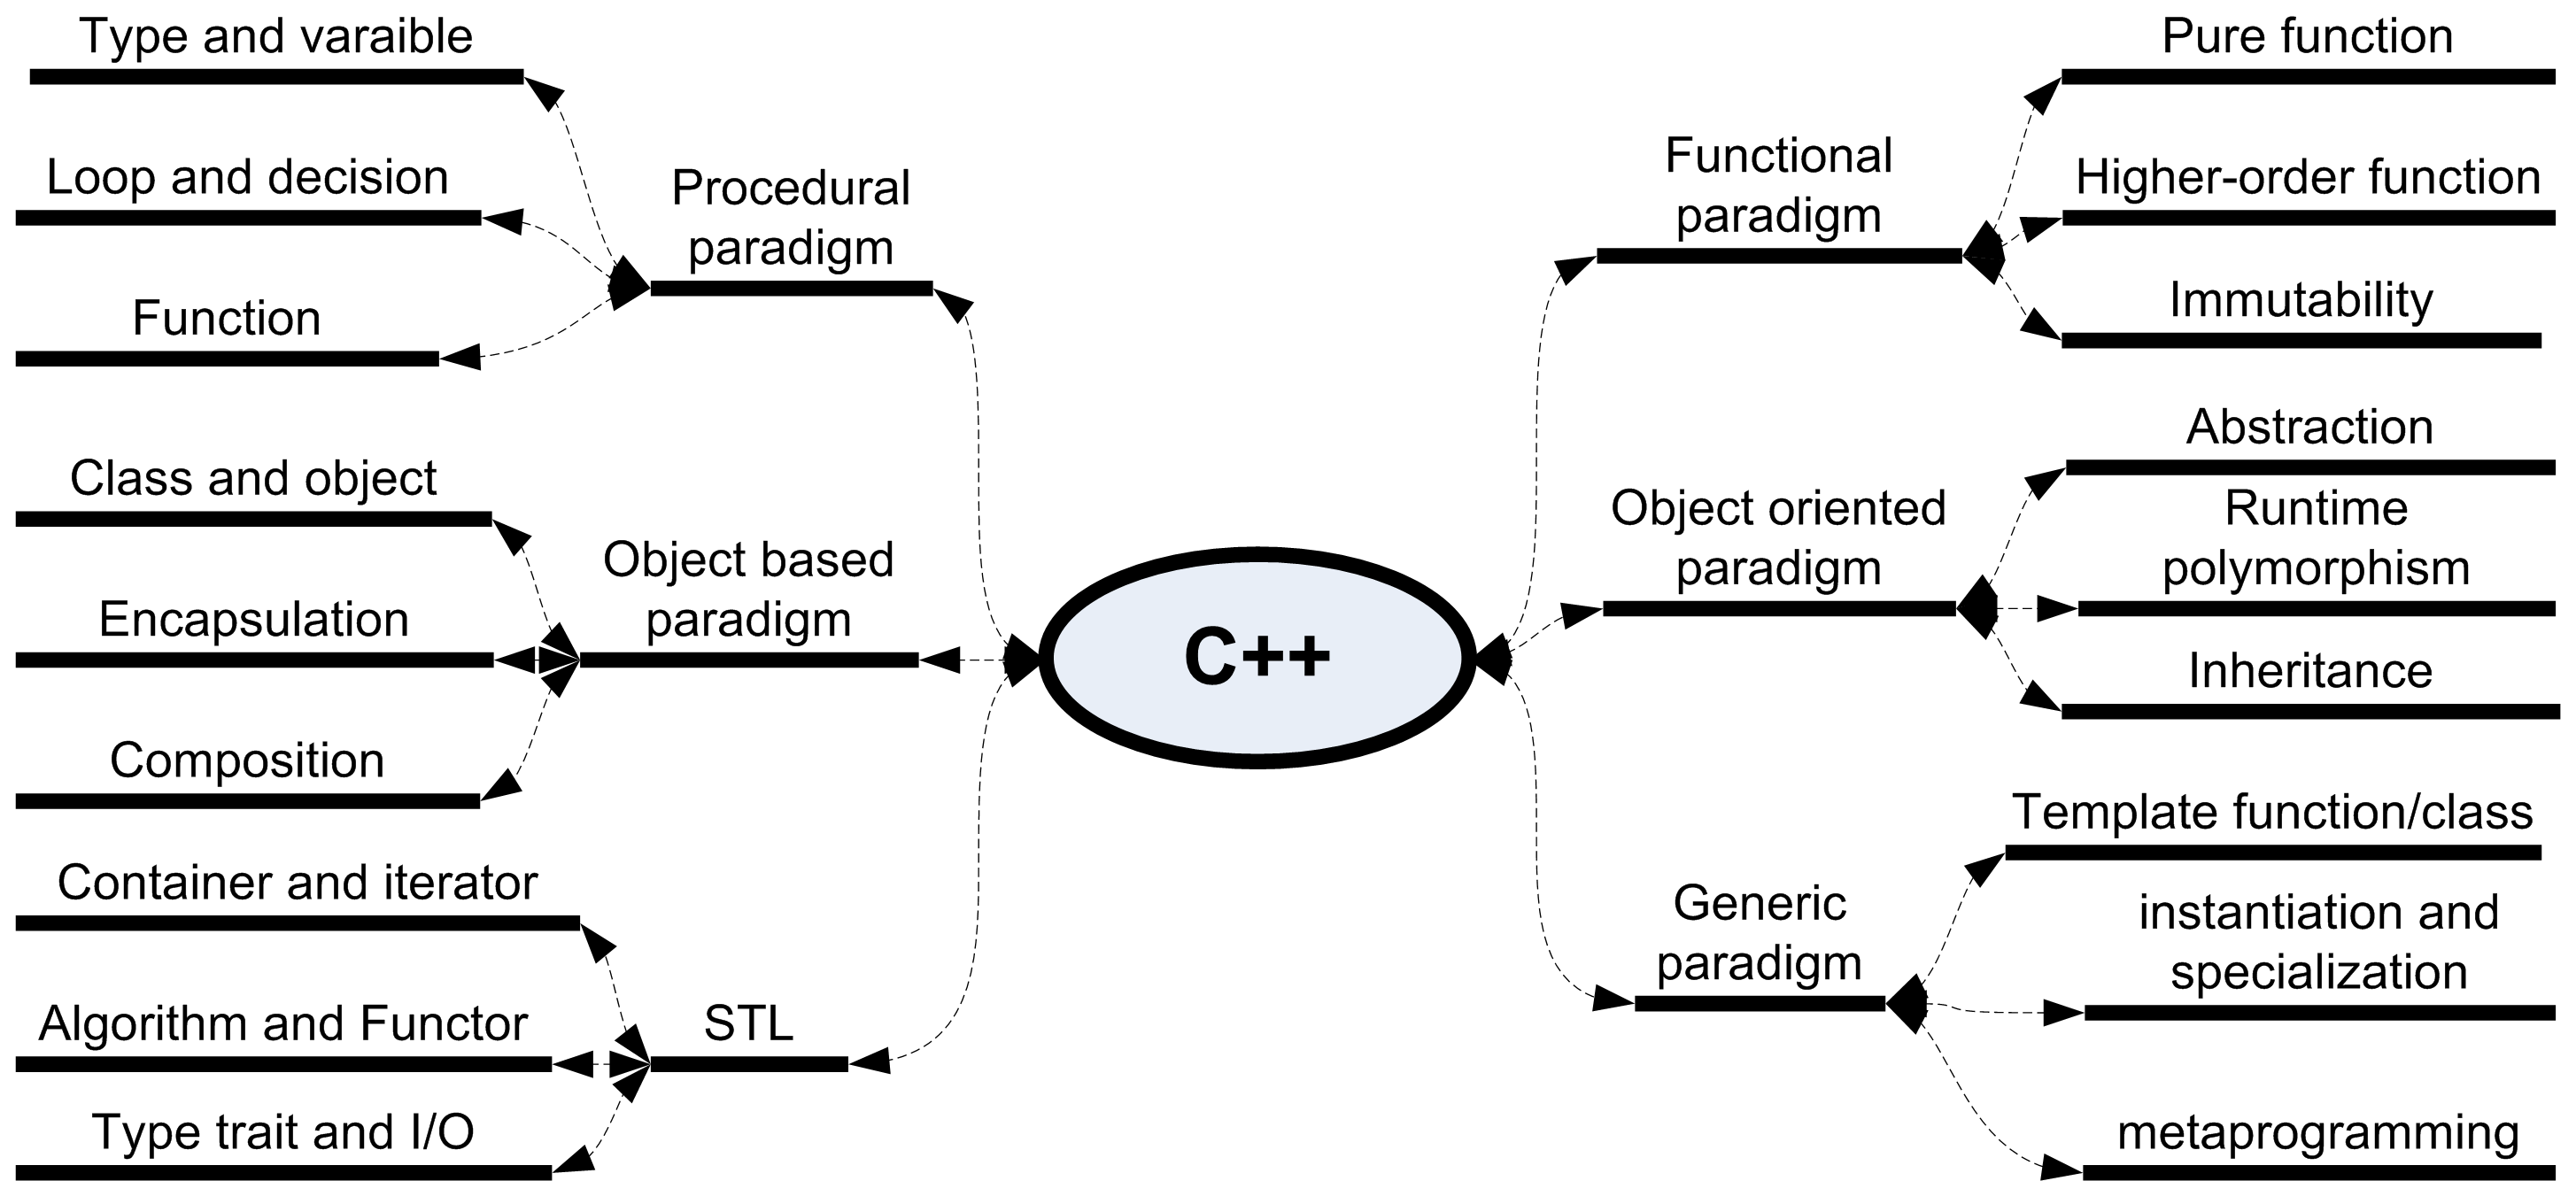
\includegraphics[width=0.95\linewidth]{pics/whole.png}
		\caption{The main components of C++ language}
		\label{fig:whole}
	\end{figure}
	
	\item About Object-base programming(data abstraction), C++ provides below supports:
	\begin{enumerate}
		\item Member function and private member data, and opy control.
		\item Global function overload, such as \texttt{complex sin(const complex\& x)} and operator overload, such as +, x, etc..
		\item template, such as \texttt{std::vector}, \texttt{std::complex}, \texttt{std::pair}.
	\end{enumerate}
	
    \item There are three constraints in C++ language: 1) compatible with C; 2) zero overhead abstraction; 3)static type. Some people also think the third constraint is value semantic. If you want to follow value semantic, you need to know the type information when you compile. So static type and value semantic are the two sides of one coin. These three constraints give C++ language very special characteristics. 
    
    \item In C++ language, value semantics refer to the way that values (i.e., objects) are passed between functions or copied from one object to another. When a value is passed to a function or copied to another object, a new copy of the value is created. Any modifications made to the copy will not affect the original value. This is in contrast to reference semantics, where a reference (i.e., pointer) to the original value is passed or copied, and any modifications made to the reference will affect the original value. The shortcoming of value semantic is less efficient than reference semantics, particularly when working with large objects or arrays. Another disadvantage is you can't change the type(static type) and type must be known at the compile time.
    
    \item \texttt{complex, pair, vector, list, map, string, stack, queue} in STL are based value semantics. They are a kind of data and support copying. 
\end{itemize}


\section{Compilation and link}

\subsection{Separate compilation and header file}
\begin{itemize}
	\item C++ uses separate compilation, which means that each source file is compiled independently and then linked together to create the final executable file. This is because C++ allows for modular programming, where large programs can be divided into smaller, more manageable units. Each unit can be developed and tested independently, and changes to one unit do not necessarily require the recompilation of other units. Additionally, separate compilation allows for faster compilation times and can help manage complexity in large codebases.
	
	\item When you write a single source file (.cpp, .cxx, etc), your C++ compiler generates a translation unit. That is to say, each .cpp will become a \textbf{translation unit.} This is the object file from your source file plus all the header files which we use \texttt{\#include} statement in the source file.  A translation unit roughly consists of a source file after it has been processed by the \texttt{preprocessor}, meaning that header files listed in \texttt{\#include} directives are literally included, sections of code within \texttt{\#ifdef} may be included, and macros \texttt{\#define} have been expanded.
	
	\item Since a C++ file is compiled \textbf{independently}, when the compiler compiles a.cpp and it uses a function or a type defined in other C++ files, it needs to know the information about those functions or types. That is why we need declarations, which are usually located in header files.
	
	\item Even though you can declare a variable, function, or class multiple times, it's not a good practice to copy declarations to other positions in other .cpp files. This leads to duplications, which are a bad smell in the code. If you modify a declaration, you would need to trace back all the other declarations. If you need to use a function or variable in many different files, you should put them in a header file. For example, you can create an \texttt{export\_to.h} file for a specific cpp source file, or a \texttt{global.h} file for the entire system. When you search for function or variable declarations globally in a project, if you find the same declaration statement more than twice, it's a strong indication that you should create a global header file and put those declaration statements in it.

	
	\item If you only want a function or variable to be visible within the current translation unit, you can declare it as \texttt{static} or use an unnamed namespace. You don't need to put it in a header file. Just remember that in C++, you have to declare a function or variable before you use it for the first time. This is different from C, where the compiler will guess a function prototype from its usage, but this is not considered good coding style in most cases for C++.
	
	\item A better suggestion would be to have a single \texttt{global.h} file for a complex system and include common types, defined types, constants, and global functions in this file. This approach can help reduce duplications.
	
	\item Some good suggestions to write a header file:
	\begin{enumerate}
		\item "Everything" that should be exported (i.e., used in other files). "Nothing" that causes the compiler to immediately generate code.
		
		\item Use \texttt{\#pragma once} to add include guard, It's not standard, but it has been supported by many main stream compiler, such as: g++, clang and MSVC.

		\item \texttt{const}, templates and inline functions are considered to have internal linkage unless explicitly marked as external using the \texttt{extern} keyword. Therefore, you should put template and inline function definitions in a header file. It's also good practice to put a semicolon at the end of the header file because you need a semicolon after declaring a class. In the .cpp file, there is no need for a semicolon after each function definition.

		\item You should put the minimal set of \texttt{\#include} statements that are needed to make the header compilable. You can use forward declaration instead of including another header file, or use a more complicated PIMPL to achieve a minimal set of other \texttt{\#include} statements in a header file. This decreases dependence.
		
		\item Basically, you should put each class definition into a single .cpp file, and make sure that each .cpp file has a corresponding .h file.  If two classes are highly correlated or very short, they maybe be put in the same .cpp file.

        \item \textbf{Don't} put "using directives" into the header files.
	\end{enumerate}

	\item Include header file in the following order. \textbf{Put your local/private header file in front of system header file. From specific to generic.} 
	\begin{enumerate}
		\item The prototype/interface header for this implementation (ie, the .h/.hh file that corresponds to this .cpp/.cc file).
		\item Other headers from the same project, as needed.
		\item Headers from other non-standard, non-system libraries (for example, Qt, Eigen, etc).
		\item Headers from other "almost-standard" libraries (for example, Boost)
		\item Standard C++ headers (for example, iostream, functional, etc.)
		\item Standard C headers (for example, cstdint, dirent.h, etc.)
	\end{enumerate}
	
    \item Why do we need to follow previous order?  This order makes some potential fault can be found as early as possible. Please see the below two examples, it demonstrates the same idea:\textbf{explicit error is better than implicit success.}
	
	\begin{enumerate}

			\item When your local/private header is included on the first place, it makes your header file self-sufficient and self-sufficient avoids hidden dependency. We should include \texttt{Boo.h} the first place, because it makes compiling fail. If we include \texttt{Foo.h} first, although compile successively, it makes hidden dependency to \texttt{Foo} invisible, that is bad code smell. 

\begin{lstlisting}[numbers=none]
Foo foo;  //hidden dependency here //Boo.h
class Boo{
  ...
}

#include Foo.h //Boo.cpp
#include Boo.h 
\end{lstlisting}
			
			\item Sometimes, if you have your own function with same name as system or library, It can give you a compiler error; Below example will give you a compiler error. But if you put \texttt{<cmath>} before \texttt{myHead.h}. Then, main will use acos in cmath, and your acos will be override. The reason behind of this failure comes from \texttt{extern "c"}.
		
\begin{lstlisting}[numbers=none]
#include "myHead.h"  //double acos(double)
#include <cmath>
main{
	acos(0.5);
}

extern "C" double acos(double);
double acos(double); // compiler accept this order declaration.

double acos(double);   // compiler report error if it sees this order.
extern "C" double acos(double); 
\end{lstlisting}
    		
	\end{enumerate}

	\item From the above code, we can see a potential issue of header file is that multiple definitions of the same function or variable can occur if header files are not properly guarded against multiple inclusions. This can lead to errors and undefined behavior.
	
	
	\item You can google "Advanced Software Engineering with C++ Templates". The first half part introduces separate compilation very well.
\end{itemize}

\subsection{Declaration and definition}
\begin{itemize}
	\item A declaration introduces an identifier and specifies its type, whether it is a type, object, or function. It is required by the compiler to allow references to the identifier.
	
\begin{lstlisting}
extern int bar;  //extern keyword before variable name, it's declaration,
extern int g(int, int); 
double f(int, double); //extern can be omitted for function declarations.
class Foo; //Foo foo is definition, No extern is allowed for type declarations.
\end{lstlisting}
	
	\item A definition actually instantiates(implements) this identifier. It's what the linker needs in order to link references to those entities. These are definitions corresponding to the above declarations:

\begin{lstlisting}[numbers=none]
int bar;
int g(int lhs, int rhs) {return lhs*rhs;}
Foo foo {}; //put {}; after class definition.
\end{lstlisting}
	
	\item The difference between declaring a symbol and defining a symbol:
	\begin{enumerate}
		\item A declaration informs the compiler of the presence of a symbol and enables referring to it wherever explicit memory address or required storage of that symbol is not necessary. On the other hand, a definition provides the compiler with information about the contents of a function's body or how much memory to allocate for a variable.
		
		\item A symbol may be declared many times in different translation unit, but defined in on translation unit only once. For example, you can forward declare a function or class as many as  you want, but you may only ever have one definition for it. This is called the \textbf{One Definition Rule}.
	\end{enumerate}

\end{itemize}


\subsubsection{Forward declaration}
\begin{itemize}
	\item In C++, we have the option to forward declare a symbol, which involves declaring its type and name, so we can use it in places where its definition is not necessary. There are three common use cases for this feature, as outlined below:
	\begin{enumerate}
		\item It will reduce compile-time dependencies --PIMPL.
		\item Hide all the implementation detail. 
		\item Break cyclic references
	\end{enumerate}
	
\begin{lstlisting}[numbers=none]
class C1; //That is a forward declaration.
class C2{
...
	C1* pc1; //A pointer, so we don't need to know the memory layout
}
\end{lstlisting}
	
	\item Forward declaration doesn't work if you need to build or access its member. It's only work when you refer it by pointer or reference. You need to write \texttt{\#include Foo.h}, so compiler can know the size and layout of \texttt{Foo} to compile below code.
\begin{lstlisting}[frame=single, language=c++]
class Foo; 
Foo* f1 = new Foo; //error,
	
fun(Foo* f1){
	f1->a;   //error, Compiler need to know if there is member a inside of Foo
}
fun(Foo f1)       //error, It's not a pointer or reference type.
\end{lstlisting}
	
	\item About cyclic include, you need to know below:
	\begin{enumerate}
		\item You can't write the code below, because it has cyclic dependent of \texttt{a.h} and \texttt{b.h}.
\begin{lstlisting}[numbers=none]
#include "b.h" //a.cpp file
class A{
	B b;
}

#include "a.h" //b.cpp file
class B{
	A a;
}
\end{lstlisting}

		\item In the end, you can use forward declaration to remove \texttt{\#include} statement. But at this time, you have to use pointer or reference in one class.
\begin{lstlisting}[numbers=none]
//a.h file, Don't need to include header file, because we use pointer later.  
class B; 
class A{
	B* b;
}
\end{lstlisting}
	\end{enumerate}
	
	\item About PIMPL(pointer to implementation), you need to know below:
	\begin{enumerate}
		\item Base on forward declaration which is introduced before, you can use "Pimpl" idiom.
\begin{lstlisting}[numbers=none]
class Widget { // "widget.h" file
private:
	struct Impl; // forward declaration here.
	Impl* pImpl;
};
		
#include "Foo.h"  // widget.cpp file, include Foo.h
struct Widget::Impl {
	Foo f1;
	...other detail.
};
\end{lstlisting}
		
		\item Pimpl Idiom is one of \texttt{std::unique\_ptr} most common use case. But just like using raw pointer,  you should define destructor even you have used \texttt{std::unique\_ptr}. 
		
\begin{lstlisting}
class Widget {     // widget.h file
	Widget::~Widget()
	
private:
	struct Impl; // Forward declaration.
	std::unique_ptr<Impl> pImpl;
};
		
#include "Foo.h"    //widget.cpp file
struct Wideget::Impl{
	Foo fo; 
}
Widget::~Widget() = default; 
\end{lstlisting}
\begin{description}
	\item[Line 2:] If you don't declare destructor here, compiler will produce default destructor in line 7 by itself, In the end, it will call \texttt{delete struct* pIm} and \texttt{struct* pIm} is a uncompleted type(definition is still invisible here)
	
	\item[Line 13:] Here, \texttt{Widget}'s destructor can see the whole \texttt{Impl} definition(line 12), so \texttt{delete struct* pIm} is legal now. You don't need to define \texttt{Widget} destructor by youself, using default one is enough.
	
	\item[Source code:] The entire idea is to control when the compiler generates the destructor for Widget; It should not be generated too early. Instead, we should wait until we have seen the complete definition of \texttt{Impl}.
\end{description}

\end{enumerate}

\end{itemize}

\subsection{Linkage}

\begin{itemize}
	\item For C language, there is tentative definition rule. You can define the same variable in two different .c file. The result will be undefined behavior. In the C++, Lucky, it is not legal any more. 
	
\begin{lstlisting}[numbers=none]
int g_i = 100;  //a.c file
//--------------------
int g_i;   //b.c file
fun(){
	printf("%d",g_i) //will print 100
}
\end{lstlisting}
	\begin{description}
		\item[gcc:] (gcc a.c b.c) report no error. in b.c, if you write \texttt{g\_i= 2}; gcc reports error.
		\item[g++:] (g++ a.c b.c) reports error.
	\end{description}

	\item In C++ language, tentative definition of variable is not allowed. At the same time, multi-definition of function is not allowed either. In the same unit, you can't define class \texttt{Foo} again, but if you put two classes \texttt{Foo} in two different .cpp file. compiler doesn't complain at all. When you run the application, it probably crashes and it's dangerous. It's a little different with function and global variable, because function and global variable all need allocate memory.
	
	\item You need to follow this principle: Either a name is for everyone (and declared in a header file) or is translation-unit-local in an anonymous namespace. Detail can be found in "The One-Definition Rule  Andrzej's C++ blog".
\end{itemize}

\subsubsection{Duration, Scope and Linkage}
\begin{itemize}
	\item \textbf{Duration} and scope are two different conceptions in C++. there are three kinds of duration: \textbf{automatic, static and dynamic.}
        \item There are mainly three kinds of \textbf{scopes}:
	\begin{enumerate}
		\item global: In C++, we can use namespace to add more scopes to divide global scope.
		\item .cpp file: (translation unit).
		\item local: function local and class local. 
	\end{enumerate}

	\item Scope is a property handled by compiler, whereas linkage is a property handled by linker. There are two linkages: internal linkage and external linkage. Internal linkage refers to everything only in scope of a translation unit. External linkage refers to things that exist beyond a particular translation unit. In other words, accessible through the whole program, which is the combination of all translation units. Linkage refers only to elements that have addresses at link/load time; thus, class declarations and local variables have no linkage. \textbf{Only global scope variable or function definition has external or internal linkage. } Some internal and external linkage examples are:
	
\begin{enumerate}
	\item non-const global variable has external linkage. Use \texttt{static} to make it internal linkage. Please pay an attention here: \texttt{static} has two usages, in file scope, it says that a variable has \textbf{internal linkage}, in function or class scope, it says that this varaible has \textbf{static duration}.
	
	\item Const global variables have internal linkage by default.
	
	\item Functions have external linkage by default. \textbf{static function has internal linkage too}. Inline function will be introduced in the next section. 
\end{enumerate}

	\item \textbf{const variables internally link by default} unless otherwise declared as \texttt{extern}. It means that:
	\begin{description}
		\item[Many copies:] You can put \texttt{const int g\_num = 10;} into a header file or global.h file. Then when you need \texttt{g\_num,} just include this header file into you .cpp and it will not cause "multiple definition" linkage error. But most of time, const global variable are used in below context to avoid linkage error. 
\begin{lstlisting}[]
//a.cpp
const Buffer_Size = 10;
int a[Buffer_Size]

//b.cpp
const Buffer_Size = 20;
int b[Buffer_size]
\end{lstlisting}
		
		\item[One copy, global access:] You also can put \texttt{const int g\_num = 10;} in one .cpp file. then declare \texttt{extern const int g\_num ;} in global.h file.\textbf{Once you use extern to declare const, you change it to external linkage.} 
		
\begin{lstlisting}[numbers=none]
//file.h:
extern const int a_global_var; 

//file.c:
#include "file.h"
const int a_global_var = /*const expression */;
\end{lstlisting}

		\item[One copy, local access:] If you really want to make const used just in one .cpp locally, use static and put it in the .cpp file.
	\end{description}
	
	\item When a definition has internal linkage, it means that:
\begin{enumerate}
		\item You can put two same static variable name in two different .cpp file, no linkage error. (Each definition will has his own memory, \textbf{Don't apply it on the large object.})
		
		\item You can't access internal linkage definition from another .cpp file. 
		
		\item You can't use \texttt{extern} with \texttt{static}, but you can use \texttt{extern} with \texttt{const}.
\end{enumerate}

\end{itemize}


\subsubsection{Inline function}
\begin{itemize}
	\item Usage of \texttt{inline} keyword is very simple: \textbf{No matter for member or non-member inline function, put it into a header file.} Why? 
\begin{enumerate}
	\item It’s imperative that the function’s definition (the part between the \{...\}) be placed in a header file, unless the function is used only in a single .cpp file. Because compiler need to see the definition, so it can expand and insert into source code directly. In particular, if you put the inline function’s definition into a .cpp file and you call it from some other .cpp file, you’ll get an “unresolved external” error from the linker. 
	
	\item At the same time, no matter how you designate a function as inline, it is a request that the compiler is allowed to ignore: the compiler might inline-expand some, all, or none of the places where you call a function designated as inline. (Don’t get discouraged if that seems hopelessly vague. The flexibility of the above is actually a huge advantage: it lets the compiler treat large functions differently from small ones, plus it lets the compiler generate code that is easy to debug if you select the right compiler options.)
	
	\item Inline just suppress multi-definition error. It is programmer's responsibility to ensure that inline function definitions with the same name match exactly across translation units, to avoid all above bad result. You can see the best way is that putting an inline function into a header file.
\end{enumerate}
	
	\item In modern C++, inline tells the linker that, if multiple definitions (not declarations) are found in different translation units, they are all the same, and the linker can freely keep one and discard all the other ones. In another word, inline is mandatory if a function (no matter how complex or "linear") is defined in a header file, to allow multiple sources to include it without getting a "multiple definition" error by the linker.
	
	\item By default all the functions defined inside the class are implicitly or automatically considered as inline except virtual functions (Note that inline is a request to the compiler and its compilers choice to do inlining or not).
	
	\begin{enumerate}
		\item For non member function, put inline function into a header file, and when you need to use this function, include it.
		
		\item For member function, you have two options.
\begin{lstlisting}[numbers=none]
class Foo {  //option 1
public:
void method(){...};  //Give definition in the class body.
};

class Foo {  //option 2, put inline definition into the header file.
public:
	void method(); //Don't put inline keyword here
};
inline void Foo::method(){  //Put inline keyword here
	...
}
\end{lstlisting}
	\end{enumerate}
		
	
	\item Does an inline function have internal linkage? No! The explanation is a little complex, so if you don't want to go deeper, you can skip the contents below. If you are confident and like facing a challenge, read on. In fact, an inline function has \textbf{external} linkage, but inlining suppresses the multi-definition error. The linker will simply pick one and discard the others, which can be dangerous. That's why we should ensure that we have only one definition and put the inline function in a header file. Then, when we want to use it, we can simply include it. We can demonstrate that an inline function has external linkage using the code below, which involves two files: a.cpp and b.cpp.
\begin{lstlisting}
inline int foo() { //File a.cpp
	return 6;
}
void g() {
	printf("foo called from g: return value = %d, address = %p\n", foo(), &foo);
}

inline int foo() { //File b.cpp
	return 12;
}
void g();
int main(){
	printf("foo called from main: return value = %d, address = %p\n", foo(), &foo);
	g();
}
\end{lstlisting} 
\begin{description}
	\item[Line 1 and 8 without inline:] it will trigger multi-definition linkage error
	\item[Line 1 and 8 one inline:] Only on inline, because inline has external linkage, so it will trigger multi-definition linkage error too.
	\item[Line 1 and 8 two inline:] Redefining an inline function with the same name but with a different function body is illegal; however, the compiler does not flag this as an error, but simply generates a function body for the version defined in the first file entered on the compilation command line, and discards the others. Therefore, may not produce the expected results.
	\item[Delete line 8 to 10:] Compiling error, identifier doesn't found.	
\end{description}

		
\end{itemize}


\subsection{Combine C and C++}
\begin{itemize}
	
	\item There are three main topics in this section, 1) what is \texttt{\_\_cplusplus}? 2) how to understand \texttt{extern "C"}? 3) Learn how to pass a class between C and C++, and how to call member function in C? 
		
	\item When you use g++,  \texttt{\_\_cplusplus} will be defined automatically. (you can't undef it in fact.) When you use C compiler, such as gcc, \texttt{\_\_cplusplus} is not defined. At the same time, When you use C++ compiler, such as g++ to compile a C file, although file extension is .c, but g++ still use name mangling to change function name.  The conclusion is based on which compiler(g++ or gcc on Linux system) you are using, not based on source file name extension.
	
	
	\item The key idea of this section is: \textbf{\texttt{extern "C"} disable name mangling.} C++ inherits basic data type, variable name, statement, expression, operator, control flow, function, file, header file and library, array, pointer and structure from C language. C++ is superset of C, so any C programs can be compiled by C++.
	
		\item If your C++ file want to use a c function. You don't have C function source code(It is in a lib or obj file) or you don't want to recompile it( it's a very big C library). At this time, you have two methods:
	
\begin{lstlisting}
extern "C"{  // method 1, Only use C++ compiler.
	c_function(int);
	#include "old_C_header.h"
}

#ifdef __cplusplus //method 2, can use C or C++ compiler
extern "C" {
#endif
	Foo (int a, int b);
#ifdef __cplusplus
}
#endif	
\end{lstlisting}
	
	\begin{description}
		\item[Line 6 to line 12:] If you can control the header file, you can use \texttt{\_\_cplusplus + extern "C"}. it will used both in C and C++ compiler. In fact, all c lib header file, such as \texttt{math.h} follow this pattern.
	\end{description}

		\item There are two occasions which you have to use \texttt{extern "C"} in your C++ code. 
	\begin{enumerate}
		\item When you want to produce a DLL or SO. Why? because maybe your DLL or SO will be used in both C language and C++ language. Or different compiler which uses different name mangling rule.
		
		\item When the code will be used by java, python or legacy C code. 
	\end{enumerate}
	
        
	\item The C++ compiler must be used to compile main(), and must be used to direct the linking process. \textbf{Most of time, you want your C++ application to call some existing C functions,} but not reverse. If you have c and cpp source files together, you can just use g++ compile them all. You don't need any \texttt{\_\_cplusplus} syntax.  g++ compiles all files using name mangling. (look them all as c++ files). At this time file extension doesn't play a role at all.
	

%	\item If you define a function in .cpp file(You have to use g++ to compile it), and this function will be used in legacy C system, you need to use \texttt{\_\_cplusplus + extern "C".} to disable name mangling.  You can give lib and head file to C system,  and then the C system can include head file and linked to lib.
	
%	\item \textbf{In one word, if you have obj code produced by C or C++, When you want to linked it to different language, you should consider using \_\_cplusplus + extern "C" }
	
	\item Can a C function directly access data in an object(lib or so) of a C++ Class. Yes, but with some restriction. C++ class has no virtual base and virtual function. no access control. If you just want to pass a object from or to C function, you can refer a article in "C++ FAQ, 36.05". It demonstrate how to pass object from main to cppCallingC (C++ to C), then call cCallingC++(C to C++). You need to pass the class pointer and use the same header file, but use \texttt{\#ifdef \_\_cplusplus} to defines one class(used by C++) and one struct(used by C), and they have the same name. Sometimes, you also need to write a C++ wrapper function, which include C++ member function syntax. Then C call this C++ wrapper function. 

\end{itemize}

\chapter{type, operator and expression}
\section{type}
\subsection{Type cast in c++}
\subsubsection{Implicit conversions}
\begin{itemize}
\item There are two kinds of conversion, one is \textbf{implicit}, and the other is \textbf{explicit}. Implicit conversions are performed whenever an expression of a type \texttt{T1} is used in context that does not accept that type, but accepts another type \texttt{T2}; in particular:
	\begin{enumerate}
		\item when the expression is used as the argument when calling a function that is declared with \texttt{T2} as parameter;
		\item when the expression is used as an operand with an operator that expects \texttt{T2};
		\item when initializing a new object of type \texttt{T2}, including a function returning \texttt{T2};
		\item when the expression is used in a switch statement (\texttt{T2} is integral type) or when the expression is used in an if statement or a loop (\texttt{T2} is bool).
	\end{enumerate}
	
	\item Implicit conversion sequence consists of the following, in this order:
	\begin{enumerate}
		\item zero or one standard conversion sequence;
		\item zero or one user-defined conversion;
		\item zero or one standard conversion sequence.
	\end{enumerate}

	\item A user-defined conversion is a conversion defined by the user, consisting of zero or one non-explicit single-argument converting constructor or non-explicit conversion operator call. You can think of the conversion operator as the opposite of a one-argument conversion constructor. For type \texttt{A}, single-argument converting constructor is \textbf{from}, and operator overload is \textbf{to}.

\begin{enumerate}
	\item Single constructor, it means that a class can be produced \textbf{from something.}
	
	\item Operator Type, it means that a class can be converted \textbf{to something.} convert class to another type, no argument, and must be member function.

\begin{lstlisting}
class A {
	A(int i); // bad style
	operator const char*(); //bad style
};

A a1, a2;
a2 = a1*2;   // implicitly convert 2 to temp A obj.
a2 = 2;   //implicitly convert 2 to temp A obj, then call operator =;	
\end{lstlisting}	
	
\end{enumerate}


	\item Implicit conversion can be called by compiler implicitly, (means that you don't know at all). It sometimes will lead to potential ambiguity problem and result which you don't expect. more detail can be seen effective c++ item 26.
\begin{lstlisting}[frame=single, language=c++]
class A{
	A(class B&); // one method converting from A to B
};
class B{
	operator A() //Another method converting From A to B
};

void g(const A&);
B b;
g(b) // Ambiguity here. two possibilities from A to B. 	
\end{lstlisting}

\item You should always \textbf{avoid} implicit conversion, and there are two rules you need to follow.
\begin{enumerate}
	\item use explicit before single parameter constructor. In the code below, with explicit keyword before constructor,  you have to use \texttt{A(2)} or \texttt{(A)2} to explicitly build a a temporary obj in \texttt{a1*A(2)} expression. It's a good habit and you should follow. 
	
	\item use name convert function instead of  "operator Type". So string class in STL has a function \texttt{c\_str()} instead operator \texttt{char*()} const. 
\end{enumerate}
\begin{lstlisting}[numbers=none]
class A {
	explicit A(int i);     // good style, explicit
	const char* getInternalPoint(); //good,a name function.
};	

A a1;
a2 = a1*A(2) // a2 = a1*2 will fail. 	
\end{lstlisting}	


		\item If you still want to use conversion operator, it is generally recommended to make conversion operators explicit to prevent implicit conversions that may lead to unexpected behavior and errors in your code. An explicit conversion operator requires an explicit conversion syntax to be used in order to perform the conversion, rather than allowing the compiler to automatically perform the conversion. This makes the code more clear and easier to understand, especially for those who may be unfamiliar with the codebase.
\begin{lstlisting}[numbers=none]	
struct X {
	operator int() const { return 7; } 	//implicit conversion
	explicit operator int*() const { return nullptr; } // explicit conversion
	
	int* p = static_cast<int*>(x); // OK: sets p to null
	//  int* q = x;  //Error: no implicit conversion	
	//   Error: array operator not allowed in conversion-type-id
	//   operator int(*)[3]() const { return nullptr; }
	
	using arr_t = int[3];
	operator arr_t*() const { return nullptr; } // OK if done through using
	//operator arr_t () const; // Error: conversion to array not allowed
};
\end{lstlisting}	
	
	\item An practical usage conversion operator can be seen in the below code. In line 8, \texttt{ref(a)} return a \texttt{reference\_wrapper} type object. so in line 3, when we use \texttt{++a}, it becomes \texttt{++reference\_wrapper}. As a result \texttt{a} (type is \texttt{reference\_wrapper}) is used in context "used as an operand with an operator that expects \texttt{T2}", so compiler can perform implicit conversion. Then it looks for "zero or one non-explicit single-argument converting constructor or non-explicit conversion function call", In the \texttt{reference\_wrapper}, we have defined \texttt{operator T\& () const}, which converts the \texttt{reference\_wrapper} to an \texttt{int\&} type, which supports the increment operator (\texttt{++}). This is the entire process. 
\begin{lstlisting}[]
template<typename T>
void functest(T a){
	++a;
}

int a = 1;
functest(a);  //a is still 1
functest(ref(a)); // a is 2 now.	 
\end{lstlisting}		
\end{itemize}

\subsubsection{Type cast operator}
\begin{itemize}
	\item Unrestricted explicit type-casting allows to convert any pointer into any other pointer type, regardless of the types they point to. While the syntax and compiling may be correct, this can lead to run-time error. In order to overcome this problem in C++, we introduce c++ cast operator, There are five cast operators, \texttt{dynamic\_cast}, \texttt{const\_cast} and \texttt{static\_cast}. It's important to always use them in C++. \texttt{reinterpret\_cast} and \texttt{bit\_cast} are not used very often. It mainly used in some specific contexts, such as compiler development.
\begin{lstlisting}[frame=single, language=c++]
char c = 10;    
int *p = (int*)&c;  //compile succeed here
*p = 5;             //but run time error later and cause stack corruption.
	
int *p = static_cast<int*>(&c); //compile fail here, more safe. 
\end{lstlisting}
		
	\item \texttt{void*} type can be converted to any other type implicitly. You don't need any cast operator when you change any type pointer to \texttt{void*}, But when you want to use dereference \texttt{void} pointer , you'd better use \texttt{static\_cast }to change it back to a certain type pointer.
\begin{lstlisting}[frame=single, language=c++]
int* p = malloc(sizeof(int)); //malloc return void*, can assign to int* in C
int* p = static_cast<int*>(malloc(sizeof(int))); //In C++, have to use cast
\end{lstlisting}		
		\begin{description}
			\item[Line 2:] In C++, you have to use cast operator. A better way is to use \texttt{new} instead.
		\end{description}

	\item Changing the value of an const object through \texttt{const\_cast} pointers leads to  "undefined behavior". For const static data -- the compiler may put such variables in a read-only region, the program will crash if you try to modify it.

\begin{lstlisting}[numbers = none]
const int a = 12;
int* p = const_cast<int*>(&a); //Bad style
*p = 66;  //UB	
\end{lstlisting}


	\item Using \texttt{const\_cast} is not good design. Sometimes for a const member function, you have to use \texttt{const\_cast} to change the "\texttt{this}" pointer to modify a class member. If compiler support, always use \texttt{mutable}  keyword.  Only use \texttt{const\_cast} if your compiler doesn't support \texttt{mutable}. Additionally, there may be cases where you need to pass a const object to a function that takes a non-const parameter, but you know that the parameter will not be modified inside the function. The second condition is important, because it is always safe to cast away the constness of an object that will only be read and not modified. In these cases, you can use \texttt{const\_cast}.

\begin{lstlisting}[numbers = none]
strlen( char* p);
const char* cp = "hello";
strlen(const_cast<char*>(cp));	
\end{lstlisting}

	\item \texttt{static\_cast<type-name>} is a valid expressio only if type-name can be converted implicitly to the same type that expression has.  It will stop you from changing a bird class to an unrelated apple class.  Even when converting from \texttt{int} to \texttt{double}, it is recommended to use \texttt{static\_cast<double>(i)}.  This type of cast can make it easier to find casting operations in your source code by searching for instances of \texttt{static\_cast}.".
\begin{lstlisting}[numbers = none]
int i = 11111600;
char c = i; //give warning
char c = (char)i; //no warning, because you have told compiler.
char c = static_cast<char>(i); //no warning, just like previous statement

int *p = (int* p)i //no warning, but crash when running
int *p = static_cast<int *>i //compile error, 
//That is why static_cast is better then C style const.
\end{lstlisting}

%	\item  \texttt{static\_cast} can't deal with inheritance well in C++. 
%\begin{lstlisting}[numbers = none]
%struct V {
%	virtual void f() {};
%};
%struct A : V {};
%struct B : V {};
%
%A a;
%V& v = a;
%B& b = static_cast<B&>(v); //compile OK, but it's UB.
%\end{lstlisting}
%\begin{description}
%	\item[Source code] From \texttt{V} to \texttt{B}, it's possible to downcast, so \texttt{static\_cast} succeed. But if \texttt{A} is behind reference \texttt{V}, then you will have undefined behaviour. That is why we need \texttt{dynamic\_cast}.
%\end{description}	
	
	\item A child pointer can always be directly assigned to a base pointer, which is known as an \textbf{up-cast} conversion and is a key aspect of polymorphic implementation. The \texttt{dynamic\_cast} operator is used to perform a \textbf{down-cast} of a base pointer to a child pointer. \texttt{dynamic\_cast} ensures that the down-cast is valid. \texttt{dynamic\_cast} can also be used with reference types. If the cast fails, \texttt{dynamic\_cast} will not return \texttt{nullptr} (because it's a reference), but will instead throw a \texttt{bad\_cast} exception.
	
\begin{lstlisting}
struct A {};
struct D : public A {};

D d; // the most derived object
A& a = d; // That is up-cast, dynamic_cast may be used, but unnecessary
D& new_d = dynamic_cast<D&>(a); // downcast, have to use dynamic_cast 
\end{lstlisting}	
	
	\item \texttt{dynamic\_cast} should only be used down-cast public inherited relationship. You can't use \texttt{dynamic\_cast} when it is not private or protected inherited relationship. If a class doesn't have virtual function, you can't use \texttt{dynamic\_cast} on this object either. If you frequently use \texttt{dynamic\_cast}, It can be a sign that your base class offer too little functionality, you'd better to re-design you base class API(adding more member function to base class.)
	
	\item \texttt{dynamic\_cast} can also be used in \textbf{side-cast in multi inheritance. }
\begin{lstlisting}[frame=single, language=c++, mathescape=true]
struct V {
	virtual void f() {}; // must have virtual function
};                            V
struct A : virtual V {};     / \
struct B : virtual V {};    A   B
struct D : A, B {};          \ /
                              D                    
D d; // the most derived object
A& a = d; // upcast 
B& b = dynamic_cast<B&>(a); //sidecast
\end{lstlisting}

\begin{description}	
	\item[Line 9:] That is side cast. Change \texttt{d} to \texttt{a} first(from child D to parent A), then \texttt{a} to \texttt{b}, (from child D to parent B, always succeed because \texttt{d} is behind \texttt{a}, and \texttt{d} can be changed to \texttt{b})
\end{description}
	
	\item \texttt{dynamic\_cast} different with \texttt{static\_cast}: 1) \texttt{static\_cast} check on compile time. 2) \texttt{static\_cast} doesn't use run time information, so sometimes it makes mistake.
\begin{lstlisting}[frame=single, language=c++, mathescape=true]
class A {
public:
	virtual void fun(){cout<<"base"<<endl;}
};

class B : public A {
public:
	virtual void fun(){cout<<"child"<<endl;}
};

A* pa = new B();
B* pb = dynamic_cast<B*>(pa); //OK, because B is behind base pointer pa,
B* pb = static_cast<B*>(pa);  //OK, 	

A* pa = new A();
B* pb = dynamic_cast<B*>(pa); //return nullptr, A is behind base pointer pa, 
B* pb = static_cast<B*>(pa);  //UB, that is not good. on my VS, it print "base"
\end{lstlisting}
\begin{description}
	\item[Line 15 to 17]  when \texttt{A} is behind base pointer, When you downcast to \texttt{B}, \texttt{dynamic\_cast} give you \texttt{nullptr}(warning), but \texttt{static\_cast} run into UB.	
\end{description}

	\item \texttt{static\_cast} can not be use in virtual base 
\begin{lstlisting}[numbers = none]
struct Parent {
	virtual void f() {};
};
struct Child : virtual Parent {}; //virtual keyword here.

Child child;
Parent& parent = child;
Child& other = static_cast<Child&>(parent); //compile fail, 
\end{lstlisting}

	\item About \texttt{dynamic\_cast}, "exceptional C++" item 44 give a good question and answer.
	

	\item RTTI makes \texttt{dynamic\_cast} work correctly in run time.  RTTI is a relatively new conception in C++, you should avoid using it on old C++ compiler. It has two methods: \texttt{typeid} and \texttt{dynamic\_cast}. There are two kinds of types (for the purposes of RTTI): polymorphic types and non-polymorphic types. A polymorphic type is a type that has a virtual function, in itself or inherited from a base class. A non-polymorphic type is everything else; this includes POD types and many other types too.
		
	\item \texttt{typeid} operator will return a \texttt{type\_info} class.  You need to include typeinfo.h header file. \texttt{typeid} operator also receive pointer or class name. \texttt{name} is member function of \texttt{type\_info}.
		
\begin{lstlisting}
int myint = 50;
std::string mystr = "string";
double *mydoubleptr = nullptr;
	
cout << "myint has type: " << typeid(myint).name(); //typeid is operator
cout<< "mystr has type: " << typeid(mystr).name();  // it returns type_info
cout<< "mydoubleptr has type: " << typeid(mydoubleptr).name(); 	
\end{lstlisting}		
			
		
	\item RTTI (Run-Time Type Information) has legitimate uses but is also prone to abuse, so it's important to use it carefully. Like exceptions, it can cause some loss in performance, but you can turn it off using the "-fno-rtti" flag. You may use RTTI freely in unit tests, but try to avoid it in other code whenever possible. Consider using one of the following alternatives to querying the type:
		\begin{enumerate}
			\item Virtual methods are the preferred way of executing different code paths depending on a specific subclass type. This puts the work within the object itself.
			
			\item If the work belongs outside the object and instead in some processing code, consider a double-dispatch solution, such as the Visitor design pattern. This allows a facility outside the object itself to determine the type of class using the built-in type system. Visitor design pattern can be seen in the later section.
		\end{enumerate}
		
	
	\item \texttt{reinterpret\_cast} can convert any pointer type to any other pointer type, even if they are unrelated classes. The operation results in a simple binary copy of the value from one pointer to the other. All pointer conversions are allowed: neither the content pointed to nor the pointer type itself is checked. It can also cast pointers to or from integer types. However, \textbf{DON'T USE IT UNLESS YOU HAVE NO OTHER CHOICE}. When you use \texttt{reinterpret\_cast} to change one pointer type to another, it violates the "strict alias rule" and can lead to undefined behavior.
	
	\item "strict alias rule" explanation. Under strict aliasing, the compiler writer is free to optimize the function \texttt{foo} below because incompatible types, \texttt{double} and \texttt{int}, can't alias. That means that if you do call \texttt{foo} as \texttt{foo((double *)\&anint)} something will go quickly wrong, but you get what you deserve.
\begin{lstlisting}
int anint;

void foo(double *dblptr){
	anint = 1;  //compiler developer can optimize this line.
	*dblptr = 3.14159;
	bar(anint);
}

foo((double *) &anint) // violate "strict alias rule"
\end{lstlisting}
	
	\item First off, yes, this results in undefined behavior because there is no \texttt{SomePod} object within the buffer. Objects do not spontaneously come into existence just because you want them too; The compiler determines that the store to the x subobject cannot possibly alias the object buffer, because buffer does not contain an x subobject, and no other object for which buffer might provide storage has been created since buffer was created. Therefore the compiler reasons that it can reorder the store to before its internal marker for the start of the lifetime of buffer. The store can now be deleted, because it is immediately followed by the start of the lifetime of an object in the same region of storage.
\begin{lstlisting}
struct SomePod { int x; };
alignas(SomePod) char buffer[sizeof(SomePod)];
reinterpret_cast<SomePod*>(buffer)->x = 42;
\end{lstlisting}
	
	\item To avoid previous undefined behavior with \texttt{reinterpret\_cast}, we can use \texttt{memcpy} to ensure that there are no UB issues. You don't need to worry about efficiency problems because the \texttt{memcpy} below will produce the same assembly code as the previous code while avoiding UB.
	
\begin{lstlisting}
struct SomePod { int x; };
alignas(SomePod) char buffer[sizeof(SomePod)];
SomePod temp;
memcpy(&temp, buffer, sizeof(SomePod));
temp.x = 42
memcpy(buffer, &temp, sizeof(SomePod));	
\end{lstlisting}
	
	\item If you understand previous \texttt{reinterpret\_cast} and memcpy, you can understand \texttt{std::bit\_cast} intent. \texttt{std::bit\_cast} also use memcpy inside, it also can be used in constexpr context and is a new feature of C++ 20.
	
	
	\item Conclusion of type cast operator. Four kinds of casts: 1)implicit cast, 2)C typle cast, 3)\texttt{static\_cast} and 4)\texttt{dynamic\_cast} they becomes more restricted and more safe. \texttt{const\_cast} should be used when you call legacy or old function without \texttt{const} parameter. \texttt{static\_cast} will suppress warning, and not allow (\texttt{int} ->\texttt{int *}) conversion. That is why we should always use \texttt{static\_cast}. \texttt{static\_cast} ALWAYS allow downcast,(because it's OK theoretically). That is why we need to use \texttt{dynamic\_cast}. \texttt{dynamic\_cast} only can be used with inheritance class with virtual function. 
	
\end{itemize}

\subsection{Arithmetic types}
\subsubsection{Numerical Overflow}

\begin{itemize}
	\item How to understand integer overflow problems? \texttt{x} is a position in the below figure, \texttt{x+3} means walk 3 step clockwise from \texttt{x}. \texttt{x-3} means walk 3 step anti-clockwise from \texttt{x}. The overflow only happen in the -8 position. Anytime you walk pass the -8 position, the overflow happens, no matter clockwise and anti-clockwise direction. For example, 5+4 = -7(not 9); -6-3 = 7(not -9).

	
\begin{figure}[!htb]
	\begin{minipage}{0.48\textwidth}
		\centering
		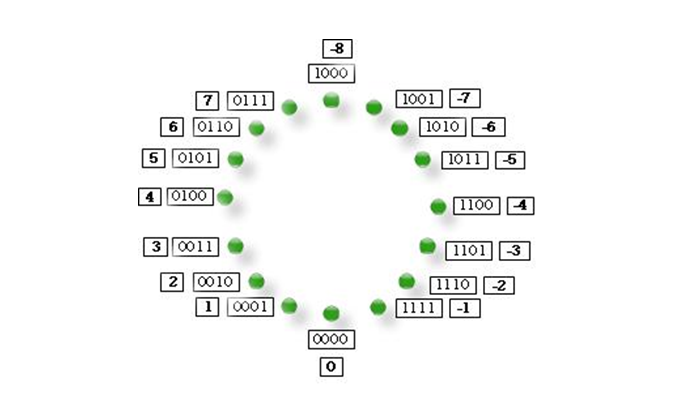
\includegraphics[width=.9\linewidth]{pics/integer.png}
	\end{minipage}\hfill
	\begin{minipage}{0.48\textwidth}
		\centering
		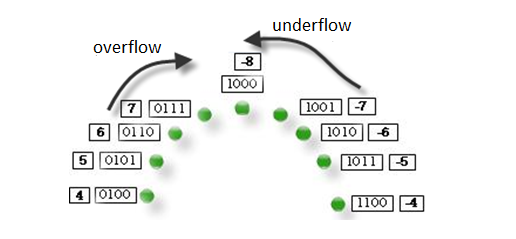
\includegraphics[width=.9\linewidth]{pics/integer1.png}
	\end{minipage}
\end{figure}


%		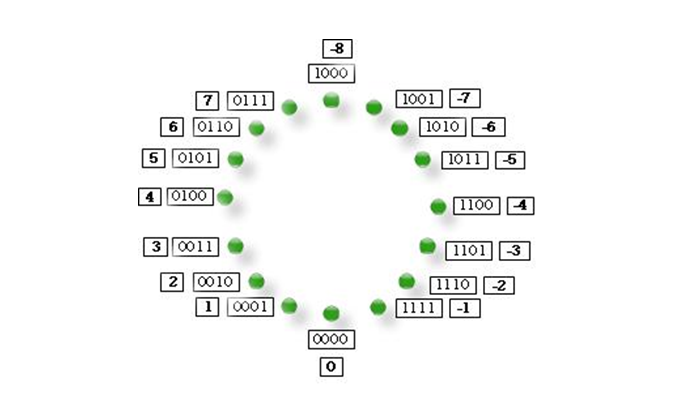
\includegraphics[width=0.5\linewidth]{pics/integer.png}		
%		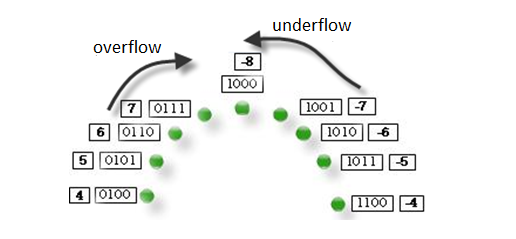
\includegraphics[width=0.5\linewidth]{pics/integer1.png}

	
	\item Integer type has \textbf{overflow} problem, and float has \textbf{precision} problem. So prefer to use \texttt{long long} and \texttt{double} as your numerical type. In modern hardware, memory usage is not big concern, and using types with enough width can save you a lot of trouble in the future. 
	
	\item In C and C++, you can use limits.h or <limit> to get all the type limit information.
	
\begin{lstlisting}[numbers=none]
INT_MAX //use in C
INT_MIN
std::numeric_limits<int>::lowest() //use in C++
std::numeric_limits<int>::max()
\end{lstlisting}
	
	\item There are three ways to deal with overflow and underflow:
	\begin{enumerate}
		\item Build your own template function.
\begin{lstlisting}[numbers=none]
template <class T>
void increment_without_wraparound(T& value) {
	if (value < numeric_limits<T>::max())
	value++;
}
\end{lstlisting}
		
		\item  Judge if overflow happens before calculation.
		
\begin{lstlisting}
if ((x > 0) && (a > INT_MAX - x)) // a + x would overflow 
if ((x < 0) && (a < INT_MIN - x)) // a + x would underflow
if ((x < 0) && (a > INT_MAX + x)) //a - x would overflow  (1-(-10))
if ((x > 0) && (a < INT_MIN + x)) //a - x would underflow (1-10)
if (a > INT_MAX / x)  // a * x would overflow 
if ((a < INT_MIN / x)) // a * x would underflow 
\end{lstlisting}
		\begin{description}
			\item[Line 1:] a is point, \texttt{x>0} means that \texttt{a+x} is clockwise turning, then it will overflow
			\item[Line 2:] a is point, \texttt{x<0} means that \texttt{a+x} is anti-clockwise turning,  so it will underflow It's easy to understand according to previous figure.
		\end{description}
		
		\item Judge it after calculation.
\begin{lstlisting}[numbers = none]
uint32 a,b;
uint32 result = a + b;
if (result < a) //overflow
\end{lstlisting}
	\end{enumerate}
	
	\item There is no simple, general, portable way to avoid integer overflow. You cannot safely check whether a signed integer addition or subtraction has overflowed after the fact. An overflow in signed arithmetic causes undefined behavior. Typically, the result wraps around, but in principle, your program could crash before you have a chance to examine the result. Clang 3.4+ and GCC 5+ offer checked arithmetic built-ins that provide a very fast solution to this problem, especially when compared to bit-testing safety checks.
\begin{lstlisting}[frame=single, language=c++]
unsigned long b, c, c_test;
if (__builtin_umull_overflow(b, c, &c_test)){
	// returned non-zero: there has been an overflow
}
\end{lstlisting}
	
	\item When you do some calculation, you can have some tricks to avoid overflow. If you  want to know the last three digits of \texttt{n!}. You need use \texttt{mod} to keep last two digits in each calculation.
\begin{lstlisting}[numbers = none]
(a+b)/2  //a+b maybe overflow
a/2+b/2 +(a&b&1); //will not overflow
\end{lstlisting}
	
\end{itemize}

\subsubsection{Numerical conversions}
\begin{itemize}
	\item Numerical conversions happen in three contexts:
	\begin{enumerate}
		\item Assign a value of one \textbf{arithmetic type} to a variable of another arithmetic type.
		
		\item Combine mixed types in expressions.(Most of time, implicit conversion)
		
		\item Pass arguments to or return from a function with different types.
	\end{enumerate}
	
	\item Converting short type to long type is \textbf{promotion}, it happens when we need hardware bit alignment optimization. Most of time, we don't need to worry about it. In an expression, C++ makes three kinds of automatic promotion conversion.
	\begin{enumerate}
		\item Some types are automatically converted whenever they occur. For example, when you add \texttt{char} to \texttt{char}. C++ converts \texttt{bool}, \texttt{char}, \texttt{unsigned char}, \texttt{signed char} and \texttt{short} to \texttt{int}. Because \texttt{int} type is generally chosen to be the computer's most natural type. \textbf{It does calculations faster for that type.} It's called \textbf{integer promotions.}
		
		\item Some type are converted when they are combined with other types in an expression. When an operation involves two types, the smaller is converted to the larger. For example, when you add an \texttt{int} to a \texttt{float}, \texttt{int} is converted to \texttt{float} type. (You have to do it, because two types have the different inside binary representations.)
		
		\item \texttt{unsigned short} convert to \texttt{int} if \texttt{short} is shorter than \texttt{int}, if they have the same size. \texttt{unsigned short} convert to \texttt{unsigned int}.  So no data loss in promoting.
	\end{enumerate}
	
\begin{lstlisting}
char c1, c2, c //c1 and c2 convert to int first.
c = c1+c2;  // then change int result back to char.

store i8 97, i8* %c1, align 1  //LLVM IR code below
store i8 2, i8* %c2, align 1
%0 = load i8, i8* %c1, align 1
%conv = sext i8 %0 to i32
%1 = load i8, i8* %c2, align 1
%conv1 = sext i8 %1 to i32
%add = add nsw i32 %conv, %conv1
%conv2 = trunc i32 %add to i8 

i+f // i will promoted to f
float f1, f2, f
f = f1+f2  
\end{lstlisting}
	
	\begin{description}
		\item[Last line:] Whether \texttt{f1} changes to double depends on compiler. clang++ has fadd in LLVM IR, so it doesn't change \texttt{f} to double.
	\end{description}
	
	\item A implicit conversion will happen when you assign value to a bool, zero converts to false, and nonzero converts to true.
	
	\item When a implicit conversion happen, assigning a value to a type with a greater range usually poses no problem. If shorter range or different type, maybe there are some problems. For example, when conversion \texttt{double -> float, long long ->float} happens, it maybe lose precision. When \texttt{float -> i} happens, it loses fragment. It even bring undefined behavior when you have below code: \texttt{int i = 666; char c = i;}.
	
\begin{lstlisting}
int i, float f = 3.99;
i=f;  //i will be 3(not rounding), UB if f is too big

f = i; //will lost precision if i is big.
\end{lstlisting}
	
	\item A implicit conversion also happen when you call a function.(Just like you use assignment operator=). Below they all compile successfully. Compile with -Wconversion flag, note that it is not included in -Wall in g++; It only gives warning when standard conversion occurs, not for promotion conversion.

\begin{lstlisting}[numbers=none]
bool isLucky(int number);

isLucky('a') // promotion ,NO warning
isLucky(false) // promotion, NO warning
isLucky(1.2f) //standard conversion.  Warning
\end{lstlisting}
	
	\item In C++, introduce braces initialization \{\}, It will not allow narrowing happen. But in g++, it just show a -Wnarrowing message, Anyway, I think that it's helpful.
\begin{lstlisting}[numbers=none]
int x = 66;  char c1 = {x}; //ok	
int x = 666; char c2 = {x};// not allowed;

int fun(){
	return 1.2f; //OK, no warning
	return {1.2f}; //ERROR, -Wnarrowing
}
\end{lstlisting}
	
	\item In order to suppress conversion warning, you can use explicit numerical conversion to state your intention clearly and loudly. In C language, there exist two main syntax for explicit type-casting: functional and C-style cast.  \textbf{Prefer C-style cast in C language}. In C++ language, \textbf{You should always use \texttt{static\_cast}}.
	
\begin{lstlisting}[]
double x = 10.3;
int y;
unsigned int n2 = unsigned(f);     // functional cast
unsigned int n1 = (unsigned int)f; // C-style cast
int b = static_cast<int>(f);  //explicit C++ style
\end{lstlisting}
	\begin{description}
		\item[Line 4:] functional cast only be used in one word type. \texttt{unsigned int (f)} is not right, \texttt{int *(p)} is not right either. That is why we prefer C-style cast in C language.
	\end{description}
\end{itemize}

\subsection{size\_t and ptrdiff\_t}

\subsubsection{Be careful with unsigned int}
\begin{itemize}

    \item When an \texttt{unsigned int} and an \texttt{int} are added together, the \texttt{int} is first converted to \texttt{unsigned int} before the addition takes place and the result is also an \texttt{unsigned int}. In another word, For integer addition or subtraction, It is just a trip around clock. When you reach a position in the clock, how to understanding depends on its context and type.
\begin{lstlisting}[numbers=none]
unsigned int ui = 1;
int i = -2;
//ui+i will be expressed 0xffffffff in memory. 
printf("%d", ui+i); //print -1.
printf("%u", ui+i); //print UINT_MAX.	
cout<<ui+i<<endl; //output 4294967260.
(ui+i)<6  //false here, interpret (ui+i) as unsigned int.
\end{lstlisting}
    
	\item You can see llvm reference. 1) has only i32, no ui32 2) has only add and mul, no uadd or umul.  3) but has uge, zext or sext, udiv. That is to say, these three operations 1)comparison, 2)promotion, 3)divid  need interpret signed or unsigned semantic differently. In order to understand why we need udiv and sdiv two different operation, just like why we need logical shift right and arithmetic shift right, because for signed and unsigned number, we need to take different action. Detail can be see \verb|https://llvm.org/docs/LangRef.html| to get more detail.
	 
\begin{lstlisting}[frame=single, language=c++]
unsigned int ui = 1 
int i = -2;
(ui+i)/4  //a big positive number
int* p;
p+(ui+i);  //OK on 32 bits platform, but crash on 64 platform.
\end{lstlisting}

\begin{description}
	\item[Line 5:] On 64 bits, \texttt{ui+i} will be promote to 64 bits first. At this time, it will be promoted according to \texttt{unsigned int}. For \texttt{p+(ui+i)} portable problem, we can use \texttt{size\_t} and \texttt{ptrdiff\_t} type. 
\end{description}
	
    \item In summary, \texttt{ui+i} result type is \texttt{unsigned int},  when you use \texttt{ui+i} in 1) compare with other, 2) promote 3) divid, it will interpret according to its unsigned semantic(non negative). Maybe it's not what you expect.  In one word, Don't use unsigned type just for big range, if int is not big, just use long, don't use unsigned int. Don't combine unsigned and signed type together.
\end{itemize}

\subsubsection{size\_t and ptrdiff\_t}
\begin{itemize}	
	\item \texttt{size\_t} is commonly used for array indexing and loop counting. Programs that use other types, such as \texttt{unsigned int}, for array indexing may fail on, e.g. 64-bit systems. \texttt{ptrdiff\_t} is used for pointer arithmetic and array indexing, if negative values are possible. Programs that use other types, such as \texttt{int}, may fail on, e.g. 64-bit systems. The main reason for using \texttt{size\_t} is that the size of something depends on a pointer, but on different systems, the size of a pointer is not the same as the size of an int. The size of a pointer is always the same as \texttt{size\_t}. The size of \texttt{size\_t} and \texttt{ptrdiff\_t} always coincide with the pointer's size. Because of this, these types should be used as indexes for large arrays, for storing pointers, for pointer arithmetic, loop counters, array indexing, and address arithmetic." 
	
	\item Type \texttt{size\_t} is a typedef that's an alias for some unsigned integer type, typically \texttt{unsigned int} or \texttt{unsigned long}, but possibly even \texttt{unsigned long long}. Each Standard C implementation is supposed to choose the unsigned integer that's big enough--but no bigger than needed--to represent the size of the largest possible object on the target platform.
	
	\item \texttt{size\_t?} can resolve portable problem. The first function work well in 16 bit OS, but in 32 bit OS, it can't copy big object(bigger than 16 bit.) The second function works well in 32 bit OS, but in 16 bit OS, it's not high efficient. The \texttt{size\_t} version can work well in both 16 and 32 bit system.
	
\begin{lstlisting}
//suppose that int is 16 bit and long is 32 bit
void *memcpy(void *s1, void const *s2, unsigned int  n); 
void *memcpy(void *s1, void const *s2, unsigned long  n);
void *memcpy(void *s1, void const *s2, size_t n);
\end{lstlisting}

	\item At the same time, using \texttt{size\_t} appropriately makes your source code a little more self-documenting. When you see an object declared as a \texttt{size\_t}, you immediately know that it represents a \textbf{size} in bytes or an \textbf{index}, rather than an error code or a general arithmetic value.
	
	\item \texttt{ptrdiff\_t} type is a base signed integer type of C/C++ language. The type's size is chosen so that it can store the maximum size of a theoretically possible array of any type. 
\begin{lstlisting}[numbers=none]
int A = -2;   // should use ptrdiff_t here
unsigned B = 1; // should use ptrdiff_t here.
int array[5] = { 1, 2, 3, 4, 5 };
int *ptr = array + 3;
ptr = ptr + (A + B); //Error on 64 bit OS.
printf("%i\n", *ptr);
\end{lstlisting}
	
	\item  A good article is "Why size\_t matters", another one is "About \texttt{size\_t} and \texttt{ptrdiff\_t"}. 
\end{itemize}

\subsection{Compound Type}

\begin{itemize}	
	\item In C, arrays are implemented as pointers to their first element. When you declare an array, you get a pointer to the first element of the array. Therefore, certain array operations can be expressed as corresponding pointer operations. 
	
\begin{lstlisting}
int arr[5] = {1, 2, 3, 4, 5}; //int * ptr = arr;
arr[1] = 3  //*ptr = 3;
\end{lstlisting}

	\item If you understand this equivalence, you can understand the following statements: An array of integers is a pointer to integers, an array of floats is a pointer to floats, an array of pointers is a pointer to pointers, and an array of arrays is a pointer to arrays. Regarding a pointer to a pointer, you can think of it as a ragged two-dimensional array. Concerning a pointer to an array, you need to know how to declare it correctly in syntax. I will discuss these two topics in more detail next. 
	
	\item A pointer to a pointer is mostly used in ragged arrays and arrays of lists. For a ragged character array, you can use a null character as an end marker, while for a ragged integer array, you need to include extra size information. If you want to modify a pointer parameter, you can use \texttt{int* \&p}; this is more clear and direct than using a pointer to a pointer.
\begin{lstlisting}
int** p = new int* [2]; //that is array of pointer.
p[0] = new int[2], p[1] = new int[3];

p[0][1] = 0;
int* &rp = p[0]; 

delete [] p[0], delete [] p[1];
delete [] p;			
\end{lstlisting}	
	
	\item Any complex declaration is either a pointer to an array or a pointer to a function. Let me introduce pointer to an array first. 
\begin{lstlisting}
int a [2] = {1, 3};
int b [3] = {1, 2, 3};

int (*p)[] ; //can omit the dimension, but you can not increment it.
p = &b; //p = &a is OK, (*p)[1] is ok, but ++p error

int (*p)[3]; //C/C++ both support int(*p)[] and int(*p)[3]
p = &b;  //p = &a is error, (*p)[1] is ok, but ++p is OK.	
\end{lstlisting}	
	
	\item When using \texttt{typedef}, the basic syntax remains the same, but the identifier becomes a type instead of a variable. It is common practice to use a capital letter to denote that the identifier is a type.
\begin{lstlisting}[]
struct Block{
	int i;
	int j;
} bb;  //define variable, bb is variable.

typedef struct Block{
	int i;
	int j;
} BB;  //define type, BB is type 	
\end{lstlisting}	
	
	\item Pointers to functions can be defined using \texttt{typedef}. This allows for easier use and readability of complex function pointer types.
	
\begin{lstlisting}
int (*foo_ptr)( int )

typedef int (*FOO_PTR_T)( int );
FOO_PTR_T foo_ptr;	
\end{lstlisting}	
	
	\item An array of pointers to functions can also be declared using \texttt{typedef}. This has the advantage of making complex function pointer types more readable and easier to use.
\begin{lstlisting}
int (*foo_ptr_array[2])( int )

typedef int (*Foo_ptr_t)( int ); //A better way is to use typedef
Foo_ptr_t foo_ptr_array[2];	
\end{lstlisting}	
	\begin{description}
		\item[1] The first step, get the variable name, look right, found that it's array. what types are in the array?
		\item[2] Then look left, found that pointer, then that is an array pointer.
		\item[3] Then look right, found that this is parentheses, that is function. so pointer to function, what type of function?
		\item[4] then look left, parameter is \texttt{int}, and return type is \texttt{int} too.
	\end{description}
	
	\item Below code is a pointer to function which returns complex type. This is a function pointer, The function input a \texttt{int} and return a pointer. The return pointer points to an array, and array's element type is \texttt{int *}.
\begin{lstlisting}
int * (* (*fp1) (int) ) [10];
//Start from the variable name -> fp1
//Nothing to right but ) so go left to find * -> is a pointer
//Jump out of parentheses and encounter (int) -> to a function that takes an int as argument
//Go left, find * -> and returns a pointer
//Jump put of parentheses, go right and hit [10] -> to an array of 10
//Go left find * -> pointers to
//Go left again, find int -> ints.	
\end{lstlisting}	

	\item The basic method for interpreting complex declarations is to start by finding the identifier name and using it as a center point to expand both to the right and to the left, following the "right-then-left" rule. A good reference is here: How to interpret complex C/C++ declarations. You can google and read it. 	
	
	\item You can also use "using alias" to simplify complex compound types, such as function pointers. By defining an alias for a complex type, you can make your code more readable and easier to understand. 
\begin{lstlisting}
using MyArray = int[10];
using MyFuncPtr = MyArray* (*)(int);

MyArray* MyFunc(int x) {
	...
}

MyFuncPtr myFuncPtr = MyFunc;
MyArray* arr = myFuncPtr(5);
	
\end{lstlisting}
\end{itemize}

\subsection{Some type categories}
\subsubsection{Aggregate}
\begin{itemize}
		
	\item \textbf{The basic idea of Aggregate type is that you can use aggregate list initialization}. All the detail definition of an aggregate can be traced back to this main purpose. In source code level, an aggregate is an array or a class with no user-declared constructors, no private or protected non-static data members, no base classes, and no virtual functions.
\begin{lstlisting}[numbers=none]
class NotAggregate1{
	int x; //x is private by default and non-static
	virtual void f() {} //remember? no virtual functions
};
		
class Aggregate1{
private:
	void f() {} // ok, just a private function
};
\end{lstlisting}

	\item In C++11, Previously, an aggregate could have no user-declared constructors, but now it can't have user-provided constructors. Is there a difference? Yes, there is, because now you can declare constructors and default them:
\begin{lstlisting}[numbers=none]
struct Aggregate {
	Aggregate() = default; 
};
\end{lstlisting}

	\item In C++11, Now an aggregate cannot have any brace-or-equal-initializers for non-static data members. What does this mean? Well, this is just because with this new standard, we can initialize members directly in the class like this:
\begin{lstlisting}[numbers=none]
struct NotAggregate {
	int x = 5; // valid in C++11
	std::vector<int> s{1,2,3}; // also valid
};
\end{lstlisting}

	\item  An aggregate class can have a non-aggregate data member. Because it will not stop us from using aggregate initialization for the aggregate class. You can see the example code below, value in brace list can be used to call non-aggregate user define constructor. So for class \texttt{Test}, it is still aggregate type.
\begin{lstlisting}[]
class Foo{
public:
    Foo(int i): i_{i}{ };
    int i_;
};

struct Test{
    Foo f;
    int k;
};

cout<<is_aggregate_v<Foo><<endl; //No, because we have user define constructor
cout<<is_aggregate_v<Test><<endl; //Yes, it can include non-aggregate.
Test t = {1,2}; //can use aggregate init here.
\end{lstlisting}

	\item Now let's see how aggregates are special. They, unlike non-aggregate classes, can be initialized with curly braces \{\}. 
\begin{lstlisting}[frame=single, language=c++]
struct X{
	int i1;
	int i2;
};
	
struct Y{
	char c;
	X x;
	int i[2];
	float f; 
protected:
	static double d;
private:
	void g(){}      
}; 
	
Y y = {'a', {10, 20}, {20, 30}}; //initialized by list initialization, f is 0
\end{lstlisting}
	
	\item Now that we know the definition of aggregates, let's try to understand the restrictions on classes; that is, why they are there. We should understand that memberwise initialization with braces implies that the class is nothing more than the sum of its members. If a user-defined constructor is present, it means that the user needs to do some extra work to initialize the members therefore list initialization would be incorrect. If virtual functions are present, it means that the objects of this class have (on most implementations) a pointer to the so-called vtable of the class, which is set in the constructor, so brace-initialization would be insufficient. 
	
	\item An aggregate is basically a simple collection of data that does not have any invariants the class would have to guarantee. Since there is no invariant and thus all combinations of possible values of the member make sense, there is no point in making them private since there is nothing to protect.
	
\end{itemize}

\subsubsection{POD, trivial and literal type}
\begin{itemize}
	
	\item For objects of POD types it is guaranteed by the standard that when you \texttt{memcpy} the contents of your object into an array of char or unsigned char, and then \texttt{memcpy} the contents back into your object, the object will hold its original value. Do note that there is no such guarantee for objects of non-POD types. Also, you can safely copy POD objects with \texttt{memcpy}.
	
	\item An aggregate class is called a POD if it has no user-defined copy-assignment operator and destructor and none of its non-static members is a non-POD class, array of non-POD, or a reference.
	
\begin{lstlisting}[numbers=none]
struct POD{
	int x;
	char y;
	void f() {} //no harm if there's a function
	static std::vector<char> v; //static members do not matter
};
	
struct AggregateButNotPOD1{
	int x;
	~AggregateButNotPOD1() {} //user-defined destructor
};
	
struct AggregateButNotPOD2{
	AggregateButNotPOD1 arrOfNonPod[3]; //array of non-POD class
};
\end{lstlisting}
	
	\item POD-classes, POD-unions, scalar types, and arrays of such types are collectively called POD-types. POD-classes are the closest to C structs. Unlike them, PODs can have member functions and arbitrary static members, but neither of these two change the memory layout of the object. So if you want to write a more or less portable dynamic library that can be used from C and even .NET, you should try to make all your exported functions take and return only parameters of POD-types.
		
	
	\item In C++ 11, The idea of a POD is to capture basically two distinct properties: 1)It supports static initialization. 2) Compiling a POD in C++ gives you the same memory layout as a struct compiled in C. So, the definition has been split into two distinct concepts: \textbf{trivial classes} and \textbf{standard-layout classes}, because these are more useful than POD. The standard now rarely uses the term POD, preferring the more specific \textbf{trivial} and \textbf{standard-layout} concepts.

	\item If this is a trivial class, then it has trivial constructor/dtor/copy/assignment. When we build, copy or destruct these type, we don't need to call these trivial ctor/copy... \textbf{but just call malloc() or memcpy()to improve efficiency.} 
	
	\item trivial class is not aggregate class, for example, it can include private non-static data member. 
\begin{lstlisting}[numbers=none]
struct Trivial4 {
public:
	int a;
private: // no restrictions on access modifiers
	int b;
};
		
struct NonTrivial1 : Trivial4 {
	virtual void f();  // virtual members make non-trivial ctors
};
\end{lstlisting}
		
	\item One property of trivial class is that it supports static initialization. Static initialization is initialization of some variable with a compile-time value such that the value ends up being "baked into" the executable image (no code needs to be actually run). Another point of triviality is that the type can be treated exactly like a fundamental type, in that objects of the type can be copied and moved with memcpy and constructed destructed without doing anything. Hence, triviality requires a type be essentially made only of fundamental types. T
\begin{lstlisting}[numbers=none]
struct Foo {
	int x;
	int y;
};
Foo foo = {0,1}; // This init happens in compiling time.
\end{lstlisting}

\item STL has some type trait class definition. 
\begin{lstlisting}[numbers=none]
	cout<<  typeid ( T ).name();
	cout<<std::is_pod  < T  >::value;
	cout<<std::is_trivial <T >::value;
	cout <<std::is_standard_layout <T>::value;
\end{lstlisting}
	
	\item If a class is trivially copyable (a superset of trivial classes), it is ok to copy its representation over the place with things like \texttt{memcpy} For example, \texttt{std::copy} use \texttt{std::is\_trivially\_copyable} as a dispatching flag to decide whether to call memcpy or call object copy constructor. and expect the result to be the same. The detail can be seen in the reference article in the end of section. 
	
\begin{lstlisting}[numbers=none]
template <class T> 
void copy(T* source, T* destination, int n, trivial_false_type){
	for (; n > 0; n--,source++,destination++){
		//call constructor
	}
}
	
template <class T> 
void copy(T* source, T* destination, int n, trivial_true_type){
	memmove(source, destination, n); //much faster here!
}
\end{lstlisting}

\item Difference between trivial and standard layout. Both standard layout and trivial can use \texttt{memcpy} safely. But trivial doesn't guarantee that it has the same memory layout with C language.
\begin{lstlisting}[numbers=none]
struct N { // neither trivial nor standard-layout
	int i; // because there is virtual destructor
	virtual ~N();
};

struct T { // trivial but not standard-layout
	int i;
private: //access control, then the compiler is free to choose a layout.
	int j;
};

struct SL { // standard-layout but not trivial
	int i;
	int j;
	~SL();
};

struct POD { // both trivial and standard-layout
	int i;
	int j;
};
\end{lstlisting}	

	\item Aggregate refers to a type that can be initialized using list-initialization syntax. This type's definition is not recursive. It describes an characteristic to support list-initialization syntax. 
	
	\item POD is trivial and standard output and it is obsolete after C++11 and it has been expanded to two distinct concepts: \textbf{trivial classes} and \textbf{standard-layout classes}.  \textbf{Trivial class is not sub-concept of POD, it's totally new definition.}  Standard-layout classes has the same layout as structs in C, so it has better portability.
	
	\item A trivial class can be created, moved, and destructed by only memory operation and without causing any side effects. This allows for improved efficiency in certain contexts, such as using static initialization, \texttt{memcpy} instead of the copy constructor, or overwriting memory to destruct it. 

	
	\item If want to compatibility with C(not only layout compatible), you must ensure that the type is trivial AND standard-layout. For data exchange via network or file, you can use a type that satisfies only trivial or standard-layout. I would recommend either aiming for both or at least standard-layout. Because with only trivial, you risk that future compiler's or a different compiler on the other side, do rearrange data members, and then a receiver may have a different layout understanding than the sender.
	
	\item Understand them from semantic, not syntactic rules. A good article about this topic is "What are Aggregates and PODs and how/why are they special?" in StackOverflow. 
	
	\item A literal type is a type that can qualify as constexpr. This is true for scalar types, references, certain classes, and arrays of any such types. A class that is a literal type is a class (defined with class, struct or union) that has a trivial destructor. And it is an aggregate type, or has at least one constexpr constructor or constructor template that is not a copy or move constructor. The detail can be found in cppreference website.
\begin{lstlisting}[]
struct A { };
struct B { ~B(){} };

cout << is_literal_type<int>::value ; //int& and int* and A true
cout << "B: " << is_literal_type<B>::value;  //false

struct point {
	point(): x(0), y(0){  std::cout << "point() called" << std::endl; }
	constexpr point(int x_, int y_): x(x_),y(y_){}
	constexpr int hypot() { return x*x + y*y; }
	private:
	int x,y;
};

static_assert( point(3,4).hypot() == 25 );
std::cout << std::is_literal_type<point>::value;	
\end{lstlisting}
	\item The reason why a literal type cannot have a non-trivial destructor is that it would prevent the type from being used in constant expressions. A constant expression is an expression that can be evaluated at compile time, and it is used in various contexts, such as initializing global or static variables or defining template arguments. If a literal type had a non-trivial destructor, it would require dynamic memory allocation and deallocation, which cannot be done at compile time. As a result, the type would no longer be suitable for use in constant expressions, and it would no longer be a literal type.

\end{itemize}


\section{Type qualifiers}
\subsection{cv-qualifier}
\subsubsection{const in function}
\begin{itemize}
	
	\item \texttt{const} must be initialized when you declare it. \texttt{static} will be initialized to default value(usually zero value) if you don't set value manually. 
	
	\item A top-level \texttt{const} indicates that the pointer itself is constant. When a pointer can point to a constant object, we refer to that \texttt{const} as a low-level const. For reference types, you cannot change the reference itself, so top-level const is always present by default, and you can only set low-level const.
\begin{lstlisting}[frame=single, language=c++]
int i = 0;
int * const p1 = &i; // const is top-level
const int *p2 = &ci; // const is low-level

const int *const p3 = p2;
const int &r = ci; //const in reference type is always low-level
\end{lstlisting}
	\begin{description}
		\item[Line 5:] C++ is essentially that \texttt{const} applies to the type to its left. However, there's an exception that if you put it on the extreme left of the declaration, it applies to the first part of the type. Right \texttt{const} modify * on its right side. Left \texttt{const} is in the first position, so it modify the first part of the type. 
	\end{description}
	
	\item \texttt{const} mainly used in three places inside of function: 1) functions parameter. 2) function return. ( just used for \texttt{const} reference, not for return value) and 3) member function.

	
	\item For value type parameters, the function signature is the same whether or not you include the \texttt{const} keyword in front of the value parameter. Including it will cause a redefinition error. For non-value parameters, top-level const is considered part of the function signature. For example, overloads like \texttt{g(int\&)} and \texttt{g(const int\&)} are two different functions.
\begin{lstlisting}[frame=single, language=c++]
int f( int );   //just one function, 
int f( const int ); // redeclares f(int)

int g( int& );  //overload, two function
int g( const int& );
\end{lstlisting}
	
	\item For \texttt{const} value type parameter in the example below, the \texttt{const} qualifier prevents code inside the function from modifying the parameter itself. Such an assurance helps you to quickly read and understand a function. Under some circumstances, this might even help the compiler generate better code. 
\begin{lstlisting}[frame=single, language=c++]
double cube (const double side){
	return side * side * side;
}
\end{lstlisting}
	
	\item Similar to the assert statement, it's important to use the \texttt{const} keyword aggressively in C++. When using a pointer or reference as a function parameter, you should always include the \texttt{const} keyword in front of it, since most of the time you don't need to modify it. If the compiler complains, you can then remove the \texttt{const} keyword. This approach will help you use \texttt{const} more effectively.
	
	\item When function return value type, don't use \texttt{const} at all. It will not allow you to use rvalue and move. 
\begin{lstlisting}[frame=single, language=c++]
const time operator+(const time &t){  //bad smell
	time temp;
	return temp.bla = bla+t.bla;
}  //because + return const, compiler doesn't use move, low efficient.

time t3(t1+t2);
\end{lstlisting}
	
	\item \textbf{When function return reference or pointer, you can use const to restrict modify it.}
\begin{lstlisting}[numbers=none]
class String{
	const char& operator[](int position) const; 
}
\end{lstlisting}
	
	\item Most of time, only index operator \verb=[]=, assignment operator and \verb|<<|, \verb|>>| return reference. For assignment operator, we only need to return \texttt{\&}.  For istream and ostream overload, you don't need return \texttt{const} at all. 
\begin{lstlisting}[numbers=none]
Array &Array::operator=(const Array &right) {
	....
	return *this; //enables x=y= 
}
\end{lstlisting} 
	
	\item Common function interface design: you can see \texttt{const} only used in pointer or reference type. You should use more \texttt{const} in your projects. 
\begin{center}
	\begin{tabular}{|c|c|c|}
		\tophline
		\textbf{type} & \textbf{read} & \textbf{write} \\ \tophline
		
		primitive (char, int, float) & pass value & pointer or reference \\ \tophline
		class, array, structure  & const pointer or reference &  pointer or reference \bottomhline
	\end{tabular}
\end{center}
	
	
\end{itemize}

\subsubsection{const in class}
\begin{itemize}
	
	\item When \textbf{const} used in class. There are four usages.
	\begin{enumerate}
		\item In \textbf{const} member function, you can't change any member variable,(If you change it, it will report a compile error). It will make const obj can invoke this function.
\begin{lstlisting}[numbers=none]
void A::fun() const{
	this->m_a = 100 // will compile error
}
\end{lstlisting}
		
		\item \texttt{const} obj can only call \texttt{const} function. But non-const obj can call ALL functions( const or non-const).
\begin{lstlisting}[frame=single, language=c++, mathescape=true]
class Fred {
	public:
	void inspect() const;  //promises NOT to change *this
	void mutate();      //might change *this
};

void userCode(Fred& changeable, const Fred& unchangeable){
	changeable.inspect();   // Okay: doesn't change
	changeable.mutate();    // Okay: changes
	unchangeable.inspect(); // Okay: doesn't change
	unchangeable.mutate();  // ERROR:
}
\end{lstlisting}

		\item If you want to return a member of a object from a const method, you should return it using reference-to-const (\texttt{const X\& inspect() const}) or by value ( \texttt{X inspect() const}). \textbf{const member method return value or const reference.}
\begin{lstlisting}[frame=single, language=c++]
class Person {
public:
	const std::string& name_good() const;  //good style
	std::string& name_evil() const;  //bad style
	int age() const;  //good style
};

void myCode(const Person& p){ //through bad interface,
	p.name_evil() = "Igor";  // change const object
}
\end{lstlisting}
		
		\item The most common use of \texttt{const} overloading is with the subscript operator. You should generally try to use one of the standard container templates, such as \texttt{std::vector,} but if you need to create your own class that has a subscript operator, here's the rule of thumb:\textbf{ subscript operators often come in pairs.} One has const, the other has not const. 
\begin{lstlisting}[numbers=none]
class Fred { /*...*/ };
class MyFredList {
	public:
	const Fred& operator[] (size_t index) const;
	Fred&  operator[] (size_t index);
};
\end{lstlisting}
		
	\end{enumerate}
	
	\item \texttt{mutable} allows you to modify a member variable in a class by a const method. Why do we need this conception? Behind "mutable", It's bitwise const and logical const. Logical const is when an object doesn't change in a way that is visible through the public interface. An example would be a class that computes a value the first time if required, then caches the result.
\begin{lstlisting}[frame=single, language=c++]
class TextBook  {
private:
	mutable int length_;
	mutable bool isValid;
public:
	void getLength() const {
		if(isValide == false){
			length_ = strlen(*p);
			isValid = true; 
		}
		return length_
	}
}
\end{lstlisting}
	\begin{description}
		\item[Line 6:] In the example above, \texttt{getLength()} is a memberwise const function that simply reads a length value without modifying it from outside the class. However, within the function, it may need to change some private member value. In this case, you can use the \texttt{mutable} keyword so that the \texttt{const getLength()} function can modify and cache a \texttt{length\_} value. A const function only restricts changes made within the function itself, and doesn't require the caller to be a const object. We declare \texttt{getLength()} as const because, logically, it only reads the value and doesn't change anything. If we didn't declare it as const, const objects wouldn't be able to call the \texttt{getLength()} function at all.
	\end{description}
	
		
	\item In summary, the \texttt{const} keyword expands outside to indicate that an object is constant and cannot be modified, and applies restraint inside to indicate that certain members or functions of an object cannot be modified. By using the \texttt{const} keyword effectively, you can write more secure and maintainable code.
	\begin{enumerate}
		\item If you declare \texttt{getArea()} const function, it will make both const obj and non-const obj can call this member function. This is good. if you don't define it as const member function, only non-const obj can invoke this function. For outside, const increase interface applicable scope.
		
		\item But inside const member function, you need to follow below rules:
		\begin{enumerate}
			\item You can't change member variable anymore, (if you really want, use mutable keyword.) 
			\item Inside const member function, it will think all member variable const, so vector will be const implicitly, return non-const iterator will be error.
			\item You have to return const reference, such as vector subscript operator. 
		\end{enumerate}
	\end{enumerate}
	
	\item when you declare mutable, you'd better use mutex to synchronize it. It's called M\&M rule in "GotW \#6b Solution". A good reference article about const is GotW 6. 
\end{itemize}
		
		
\subsubsection{const\_iterator}
\begin{itemize}
	\item \texttt{vector<int>::const\_iterator} and \texttt{const vector<int>::iterator} is like top-level and low-level const. 
\begin{lstlisting}[numbers=none]
vector<int>::const_iterator cvi;
*cvi = 12; //ERROR, can't change
cvi++;     //OK

const vector<int>::iterator vi;
*vi = 12; //OK
vi++;     //ERROR
\end{lstlisting}

	
	\item A const \texttt{vector} obj only can call const member function, and const member function just return const reference or pointer.

\begin{lstlisting}
iterator begin() noexcept;
const_iterator begin() const noexcept;

const vector<int> cvi;
vector<int>::iterator vi = cvi.begin(); //Compile error
auto vi = cvi.begin(); //use auto to resolve this error	
\end{lstlisting}

\begin{description}
	\item[Line 5:] \texttt{cvi} will call the second overload function anyway. but second just return \texttt{const\_iterator}. and \texttt{const\_iterator} can NOT be converted to iterator implicitly.
\end{description}

	\item Continue with previous item. If you define a const obj or you have const member function, all the member variable of const obj or inside const member function is const. For example, because \texttt{getArea} is const funciton, when it is called by a const obj, points will become a const member variable, so error will happen below: 

\begin{lstlisting}[frame=single, language=c++]
class A{
	getArea() const{
		vector<int>::iterator vi = points.begin(); 
		//How to fixe, use 1) vector<int>::const_iterator vi or 2) auto vi
	}
	
	calArea(){
		vector<int>::iterator vi = points.begin();
	}
	vector<int> points
};

const A ca;
ca.calArea(); // not compile, const obj can't call non-const member	
ca.getArea(); // Not compile, points is const implicit.

A a;
a.calArea(); // non-const obj can access non-const member fun
a.getArea(); // non-const obj can also access const member fun.	
\end{lstlisting}

\begin{description}
	\item[Line 2:] because \texttt{getArea} is const member function, so \texttt{points} are const implicit. you have to use \texttt{const\_iterator} here	
\end{description}
	
	\item In C++11/14, we add \texttt{cbegin} for STL container, Some interfaces of container has changed from non-const iterator to const iterator, so we should use const iterator more. 
\begin{lstlisting}
iterator insert(iterator position, const value_type& val);//c++98
iterator insert(const_iterator position, const value_type& val);//c++11

vector<int> values:
auto it = std::find(values.cbegin(),values.cend(), 1983);
values.insert(it, 1998);
\end{lstlisting}
	\begin{description}
		\item[Line 1:] In C++98, insert doesn't support \texttt{const\_iterator} interface.
		
		\item[Line 2:] In C++11, insert interface has changed. Because insert will not change the input iterator,(it only insert a new element after input iterator, but not change input iterator directly.) so it should be \texttt{const\_iterator}.
		
		\item[Line 5:] \texttt{std::find} is generic algorithm, it just receive a template parameter,  You should provide \texttt{const\_iterator} to it, But how can you get \texttt{const\_iterator} from a non const container. After C++11, you can use cbegin to get \texttt{const\_iterator} easily.
	\end{description}
	
	\item We can't remove constness from \texttt{const\_iterator} by using \texttt{const\_cast}. If they are vector or string, maybe it's OK, because they just use pointer behind the scene. Usually, \texttt{const\_iterator} and \texttt{iterator} are two different classes. A good way is to use \texttt{std::advance} and \texttt{std::distance}. Detail can be found in effective STL. 
\begin{lstlisting}[]
std::vector<int>::iterator it = v.begin();
std::vector<int>::const_iterator cit = it; //ok to get cit from it directly.

advance(i, distance<const_iterator>(i, ci)); //change ci to i. 
\end{lstlisting}

	\item Different iterators can also be transformed according arrow direction in blow figure.
\begin{center}
		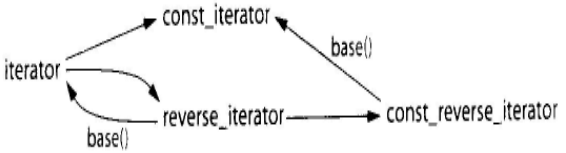
\includegraphics[width=0.6\linewidth]{pics/Iterators.png}
\end{center}
	\item Containers are required to provide iterator as a type convertible to \texttt{const\_iterator}, so you can convert implicitly:
\begin{lstlisting}	
Container::iterator it = /* blah */;
Container::const_iterator cit = it;	
\end{lstlisting}
			
	\item A good article is "effective modern C++" item 13. It introduce the basic idea about \texttt{const\_iterator.}
\end{itemize}

\subsection{constexpr}

\subsubsection{Basic definition}
\begin{itemize}
	
	\item The first concept is \textbf{constant expressions}. A constant expression is an expression that can be \textbf{evaluated at compile time}. It has many advantages, such as performance optimization and can be used in places that require compile-time evaluation, for example, template parameters and array-size specifiers.
\begin{lstlisting}
int n = 1;            //n is not a constant expression
std::array<int, n> a1; //ERROR 
const int cn = 2;     // cn is a constant expression
std::array<int, cn> a2;// OK 
\end{lstlisting}
	
	\item After C++11, by introducing \texttt{constexpr} specifier, we expand the constant expression scope. For example, a constexpr function with known parameter can be constant expression too. That is the basic idea of constexpr, If you understand this, you can understand a lot of complex syntactic knowledge below.
	\begin{figure}[h]
		\centering
		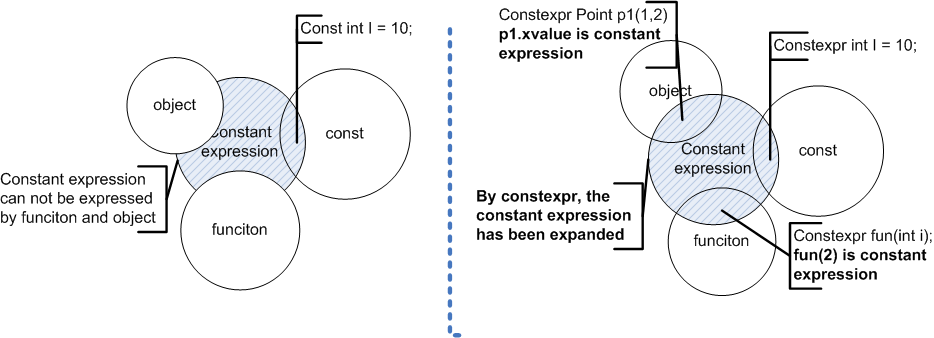
\includegraphics[width=0.9\linewidth]{pics/constexpr.png}
		\caption{Basic idea of constexpr}
		\label{fig:constexpr}
	\end{figure}
	
	\item The \textbf{constexpr specifier} declares that it is possible to evaluate the value of the function or variable at compile time. Such variables and functions can then be used where only compile time \textbf{constant expressions} are allowed (provided that appropriate function arguments are given). It has two advantages: 1) Improving efficiencies(if it's possible, it will calculate at compile time, not run time). 2) Expanding usage scope (initialize constexpr obj and use in integer constexpr context)
\begin{lstlisting}[frame=single, language=c++]
constexpr int fun(int a, int b){return a+b;}
	
constexpr int const foo = fun(2,3) ;  // without line 1 declaration, 
int a[fun(2,3)];                    //we can't use this way in line 3 and 4.
\end{lstlisting}
		
	
	\item \texttt{constexpr} can be used in three places: 1) constexpr variable, 2) constexpr obj, 3) constexpr function. constexpr function can be thought as a kind of "metafunction".
	
	\item Difference between constant expression and \texttt{constexpr}:
	\begin{enumerate}
		\item Declaring a function as constexpr does not necessarily guarantee that it will be evaluated at compile time. It can be used for such, but it can be used in other places that are evaluated at run-time, as well.
		
		\item An object may be fit for use in constant expressions without being declared constexpr. for example: \texttt{const int N = 25}.
	\end{enumerate}
	
	\item Difference between \texttt{constexpr} with \texttt{const}:
	\begin{enumerate}
		\item when you declare \texttt{constexpr} obj, it implicit \texttt{const.} But not all \texttt{const} is \texttt{constexpr.}
		
		\item \texttt{constexpr} just used on top level. If you want to specify the low level \texttt{const,} you need to write it out.
\begin{lstlisting}
constexpr int const foo = 42;
constexpr int       foo = 42; //line 1 and 2 are same 
constexpr int const *pb = &bar; 
\end{lstlisting}
		\begin{description}
			\item[Line 3:] \texttt{pb} itself is constexpr, when we initialize it, \texttt{\&bar} must be constant expression too. At the same time, \texttt{pb} points const int, it means that we can't use \texttt{pb} to change \texttt{bar}.
		\end{description}
	\end{enumerate}
	
\end{itemize}


\subsubsection{constexpr variable and object}
\begin{itemize}
	\item \textbf{All constexpr objects are const, but not all const object are constexpr}
	\begin{enumerate}
		\item constexpr variable is implicitly const. Just like const, constexpr can't be changed during run time.
		
		\item constexpr variable must be initialized when you declare it. The full-expression of its initialization, including all implicit conversions, constructors calls, etc, must be a constant expression.(You know the exact value in compiling time.)
		
		\item Value of constexpr \textbf{must be known at compile time}.If you want to get value from a function, you have to use constexpr function to assign value to it. 
		
\begin{lstlisting}
constexpr int sum(int i, int j){
	return i+j;
}
int i,j;
cin>>i>>j;
const int result = i+j; //OK
const int ce = sum(i,j); //OK
constexpr int result = i+j;  //ERROR, can't calculate in compile time
constexpr ce = sum(i,j); //ERROR
\end{lstlisting}		
	\end{enumerate}
	
	\item For constexpr object, it must has corresponding  constexpr constructor. constructor body should be empty. You can't define constexpr object if the class has no constexpr constructor.
	\begin{enumerate}
		\item can only be invoked with constant expressions.
		\item can not use exception handling.
		\item has to be declared as default or delete or the function body must be empty (C++11).
		\item The constexpr user-defined type
	\end{enumerate}
	
	\item For class itself, it also need satisfy below:
	\begin{enumerate}
		\item can not have virtual base classes.
		\item requires that each base object and each non-static member has to be initialized in the initialization list of the constructor or directly in the class body. 
		\item Consequently, it holds that each used constructor (e.g of a base class) has to be constexpr constructor and that the applied initializers have to be constant expressions.
	\end{enumerate}
	
\begin{lstlisting}[frame=single, language=c++]
class MyInt{
public:
	constexpr MyInt()= default;
	constexpr MyInt(int fir, int sec): myVal1(fir), myVal2(sec){}
	MyInt(int i){ myVal1= i-2; myVal2= i+3; }
    constexpr int getSum() const {return ...}
    
private:
	int myVal1= 1998;
	int myVal2= 2003;
};

constexpr MyInt myIntConst1;
MyInt myInt2;
constexpr int sec= 2014;
constexpr MyInt myIntConst3(2011,sec);
int arr[myIntConst3.getSum()];
static_assert( myIntConst3.getSum() == 4025, "2011+014 = 4025" );
constexpr MyInt myIntConst5(2000); //Error, constructor is not declared as constexpr function
\end{lstlisting}
	\begin{description}

        \item[Line 6:] A constexpr class must have a constexpr constructor. If a member function needs to be used in constexpr statement, it must be constexpr too: Note, in the member function definition, the qualifier of this must be const.

		\item[Line 13 and 14:] You can declare both constexpr and non-constexpr object.
		
		\item[Line 15 and 16:] If you want to use constexpr to initialize constexpr variable, you must guarantee all the parameter are constexpr.
		
	\end{description}


\end{itemize}

\subsubsection{constexpr function}
\begin{itemize}
	\item  \texttt{Constexpr} can be used with both member and non-member functions, as well as constructors. It declares the function fit for use in constant expressions. When you declare a function as constexpr, you just tell the compiler that this function is a kind of \textbf{"pure function"}. The pure function has no state, and when you run it, it has no side effect.
	\begin{enumerate}
		\item The return value is only determined by its input values.
		\item Given input values, the return value can be calculated in compiling time. 
	\end{enumerate}
	
	
	\item The pure function has some advantages compared with ordinary funciton: Return always the same result when given the same arguments, So the function call can be replaced by the result, and the order of function call is not important.(That is why you can run it at compiling time.) But the problem is compiler itself can't judge if a function is pure function, That's why programmer come to rescue. The programmer indicate this function is a "pure" function, so compiler can \textbf{For outside} use it in another constant expression context, \textbf{For inside} calculate it in compiling time. 
	
	\item On the first sight, you should declare constexpr function everywhere, but it's not good idea either. That makes a constexpr qualifier an irrevocable design decision. You cannot remove this qualifier without an incompatible change to your API. It also limits how you can implement that function, e.g. you would not be able to do any logging within this function. Not every trivial function will stay trivial in eternity. That means you should preferably use constexpr for functions that are \textbf{inherently pure functions}, and that would be actually \textbf{useful at compile time} (e.g. for template metaprogramming). It would not be good to make functions constexpr just because the current implementation happens to be constexpr-able. In semantic level, you should have something that can be evaluated down to a constant while maintaining good readability and allowing slightly more complex processing than just setting a constant to a number. Take \texttt{max( a, b )} for example: Its a pretty simple choice there but it does mean that if you call max with constant values it is explicitly calculated at compile time and not at run time.
\begin{lstlisting}[numbers=none]
constexpr int MeaningOfLife ( int a, int b ) { return a * b; }
constexpr int meaningOfLife = MeaningOfLife( 6, 7 );
	
template< typename Type > 
constexpr Type max(Type a, Type b) {return a < b ? b : a; }
\end{lstlisting}		
		
	\item constexpr functions compile much quicker than the equivalent template-based solutions, which scale linearly with the depth of the template-recursion. Where compile-time evaluation is not necessary, using inline functions or functions with internal linkage would seem more appropriate than constexpr. Both constexpr and inline are for performance improvements, inline functions are request to compiler to expand at compile time and save time of function call overheads. In inline functions, expressions are always evaluated at run time. constexpr is different, here expressions are evaluated at compile time.

	
	\item Compared with ordinary function, constexpr functions:
	\begin{enumerate}
		\item \textbf{For outside}. is able to be used in the another constant expression(such as \texttt{constexpr int sum = cfun(2,3);} ) But it doesn't mean that it must be used in constant expression(such as \texttt{int sum = cfun(i,j);})
		
		
		\item \textbf{For inside}. constexpr function adds a lot of constraints on its implementation.
	\end{enumerate}
	
\begin{lstlisting}[frame=single, language=c++]
constexpr int cfun(int i, int j){
	return i+j;
}
int fun(int i, int j){
	return i+j;
}

int i, j;
constexpr int sum = fun(2,3);  //Error
constexpr int sum = fun(i,j);  //Error
constexpr int sum = cfun(2,3); //OK
constexpr int sum = cfun(i,j); //Error

int sum = fun(2,3);  //OK
int sum = fun(i,j);  //OK
int sum = cfun(2,3); //OK
int sum = cfun(i,j); //OK
\end{lstlisting}
	
	\begin{description}
		\item[Line 9 to 12:] For constexpr variable, only cfun with constant expression is OK.
		\item[Line 14 to 17:] For Non-constexpr variable, all fun is OK.
	\end{description}
	
	\item Even with constexpr parameter, constexpr function doesn't guarantee to be evaluated at compile time. There are three contexts in which a constexpr function \textbf{MUST} to run at compile time. That's why constexpr functions must be able to return compile-time results when called with compile-time values.

	\begin{enumerate}
		\item The constexpr function is executed in a context which is evaluated at compile time. This can be a \texttt{static\_assert} expression such as with the type-traits library or the initialisation of a C-array.
		
		\item The value of a constexpr function is requested during compile time with constexpr: \texttt{constexpr auto res = func(5);}
		
		\item a template parameter or enum or switch statement.
	\end{enumerate}
	
	\item In C++11, there are a few restrictions on constexpr functions. First, they have to be non-virtual. Second, they have to have arguments and a return value of a literal type. Literal types are the types of constexpr variables. Third, the function body must be extremely simple: apart from typedefs and static asserts, only a single return statement is allowed. For constructors, only an initialization list, typedefs, and static asserts are allowed. However, =default and =delete are also allowed.
	
\begin{lstlisting}[frame=single, language=c++]
constexpr int gcd(int a, int b){
	return (b== 0) ? a : gcd(b, a % b);
}  //use ternary to replace if
\end{lstlisting}
	
	\item In C++14. constexpr function can include: conditional jump instructions or loop instructions and more than one instruction. fundamental data types that have to be initialized with a constant expression. The arguments and the return type must be \textbf{literal types} (i.e., generally speaking, very simple types, typically scalars or aggregates)
		
\begin{lstlisting}[numbers=none]
constexpr auto gcd(int a, int b){
	while (b != 0){
		auto t= b;
		b= a % b;
		a= t;
	}
	return a;
}
\end{lstlisting}
    
	\item \textbf{Use constexpr, const and noexcept more aggressively.} This adds more compilation-time checks, gives the compiler more information to optimize better and this has the nice side effect of making you think more about what you are currently doing. And remember: the longer it takes for your C++ program to compile, the greater your sense of accomplishment.

	\item A good document is "Demystifying constexpr". 
\end{itemize}

\subsection{static and volatile}
\begin{itemize}
		
	\item In C++, global and static variables are initialized to default values. However, auto variables are initialized with random values unless value initialization is used, which is not done for efficiency reasons.
		
	\item You cannot initialize a static member variable inside the class declaration; you need to put it in a .cpp file. However, if the static data member is a constant of integer or enumeration, you can initialize it inside the class declaration. If you have a constant member inside a class, it is better to use \texttt{const static} because it cannot be changed, and all objects can share the same static value.
\begin{lstlisting}[frame=single, language=c++]
class{  //in .h file
	static int obj_num;  // you can't initialize
	const static int months = 12; // you can initialize inside the class
};

int class::obj_num = 12; //in .cpp, no static keyword anymore.	
                     //will be 0 if you don't initialize it.
\end{lstlisting}	
	
	\item static member function has two usages:
	\begin{enumerate}
		\item It can be invoked just by class name, not object instance, so you can define math class and define a lot static math function inside it.  Just like namespace.
				
		\item A static function cannot access class data members, only class static member data, because static functions do not use the \texttt{this} point
	\end{enumerate}
	
	\item static can be used restrict the scope.(internal linkage) After C++ 11, static variable inside a function is thread safe, so it's an important improvement for singleton pattern.
\begin{lstlisting}[frame=single, language=c++]
int global = 0;  //All files
static int s_i = 50; //just in this file
main(){
	static int s_i = 100;  //just in this block
	printf("%d %d", ::s_i, s_i); //print 50 and 100
}
\end{lstlisting}
	\begin{description}
		\item[Line 5:] Not conflict, but if you define int \texttt{s\_i} in global scope it will conflict.
	\end{description}
	
	\item Summary: The usage of static in C++ depends on where it is used, as it can be used to declare static member variables, static member functions, and local static variables, each with different implications for the scope and lifetime of the object.
	\begin{enumerate}
		\item Use it inside a function. invisible outside of function, static life time and valid until program end.
		
		\item Use it inside a class. only copy for all instances, and access by static member function.
		
		\item Use it before global variable to create an internal link and avoid name conflicts. However, in modern C++, it is preferable to use an unnamed namespace.
	\end{enumerate}

	\item In C++, the volatile keyword is used to indicate that a variable may be modified outside of the control of the program. Specifically, it tells the compiler not to optimize away or cache accesses to the variable.
\begin{enumerate}
	\item When accessing hardware registers or memory-mapped I/O: In these cases, the value of the variable can change unexpectedly, so using volatile ensures that the variable is always read from or written to memory.
	
	\item When using a variable that is modified by another thread or signal handler: Without volatile, the compiler may optimize away accesses to the variable, resulting in incorrect behavior.
\end{enumerate}

\item It's worth noting that using volatile can have a performance cost, as it prevents the compiler from optimizing certain code paths. As a result, it's important to use volatile only when necessary, and to understand the potential trade-offs. Do not use "volatile" except in low-level(embedded c) code that deals directly with hardware. 
\begin{lstlisting}[frame=single, language=c++]
void waitForSemaphore(){
	volatile uint16_t* semPtr = WELL_KNOWN_SEM_ADDR;
	/*well known address to my semaphore*/
	while ((*semPtr) != IS_OK_FOR_ME_TO_PROCEED);
}		
\end{lstlisting}	

\end{itemize}


\section{Name}
\subsection{Namespace}

\begin{itemize}
	\item Don't put a lot of stuff in the global scope. Learn to use namespaces to split your global scope into different scopes. If you develop a library of functions or classes, you should put them in a new namespace, just like the std namespace in STL. Don't put your own class into the namespace std. Usually, the namespace should be your project name, and you can add your company name in front of it if you like.
		
	\item Using :: before a function name indicates the global namespace. For example, \texttt{::max} will hide \texttt{std::max}. This way, you can define your own max function in the global scope and use \texttt{::max} to call your own max function.
	
	\item Namespaces can be located at the global level or inside other namespaces. They can't be placed in a block. So it has external linkage by default, that is to say it can be accessed by multi translation unit(files). There are three ways to use namespaces. A using-declaration introduces a member of another namespace into the current namespace or block scope. It's a recommended way to use namespaces.  
\begin{lstlisting}[numbers = none]
using sp::name;   //1) using declaration, recommend
using namespace sp;   //2) using directive
sp::name   //3) specific refer it
	
namespace ns{
	int zy;
}
using std::string; //using declaration
using namespace ns;
int main(){
	string str = "abc" //don't need to use std::string.
	int zy = 0; //it will hide ns::zy
	cin>>zy; //read into local zy
}
\end{lstlisting}


	\item Don't use a using directive in any header file because it will "pollute" all the .cpp files that include this header file. If you have to use a using directive in your .cpp file, put it after all the include files. Use a using directive as little as possible in any .cpp file. Instead, use scope-resolution or using-declaration more often. This will help avoid polluting the namespace.
\begin{lstlisting}[numbers=none]
#include <iostream>
using std::cout;
using std::endl;
cout<<"Hello world"<<endl;	
\end{lstlisting}	

	
	\item For implementation code, there are four methods to put it into namespace. Method 3 and method 4 are recommended.
	
\begin{lstlisting}[numbers=none]
namespace Yan{ //a.h
	Class Foo{
		void mem_fun();
	};
}
	
using Yan::Foo;  //method 1. using declaration
void Foo::mem_fun(){.......}
	
using namespace Yan; //method 2. using directive. It's bad style.
void Foo::mem_fun(){.........}
	
void Yan::Foo::mem_fun(){.........} //method 3. It's good style.

namespace Yan{  //method 4. can include more contents inside.
	void Foo::mem_fun(){......}
}
\end{lstlisting}

	
	\item unnamed namespace just like \texttt{static} to specify its content to local file scope. At the same time, make anonymous namespace as small as possible.  see C++ primer p492.
	
\begin{lstlisting}[numbers=none]
// a.cpp file
static int count;

namespace{ // A better method to use namespace.
	int count;
}
\end{lstlisting}
	
\end{itemize}


\subsection{Name lookup}
\begin{itemize}	
	\item The function call process consists of three phases: name lookup, overload resolution, and access control. Here's a detailed explanation of each phase:
	\begin{enumerate}
		\item First, compiler looks in the \textbf{immediate scope},  and makes a list of all functions that have right names  (regardless of whether they're accessible or even take the right number of parameters). Please note, \textbf{If compiler has found function name, even the parameters don't match, compiler will not continue outward search. It stops here and barks}. It's a safe measure, compiler think the immediate scope is "priority zone". Maybe you omit parameter, compiler should not search outward implicitly. Only if compiler doesn't find any same function name at all, then compiler continue to "search outward" into the next enclosing scope and repeat.
		
		\item In the searching scope, if there are more than one candidate functions, the compiler perform overload resolution and then applying access rules. \textbf{In one word, overload resolution does not go beyond scopes!} Overload resolution has a good introduction: "C++ Primer plus" chapter 8 "Which Function version the compiler pick". The main idea is: \textbf{exact match non-template > template > argument conversion(promotion or implicit conversion)}. Compiler will first match function name and number of arguments, then look for template deducted function, then use implicit conversion to try match. \textbf{So implicit conversion happens after template.}
		
		\item If the compiler finds a suitable function definition, it checks whether the calling code has access to that function based on the function's access control level. If the calling code doesn't have access, it reports an error.
		
	\end{enumerate}
	
\end{itemize}

\subsubsection{Name searching scope}
\begin{itemize}
	
	\item There are four examples about "immediate scope".
	\begin{enumerate}
		\item class scope:
\begin{lstlisting}
void f1(int i ){...};
class Foo{
	void f1(string & str){};
	void f2(void){
		int i = 3;
		f1(i); //compiler bark here! it only see f1(string &)
	}
};
\end{lstlisting}
		
		\item Child class scope. 
\begin{lstlisting}
struct B{
	int f( int );
	int g( int );
};
		
struct D : public B{
private:
	int g( std::string, bool );
};
D d;
d.g(3); //error: g takes 2 args, In child class scope, if it found name g, then it will stop looking for another name in outward scope. then found argument number is not match, then compiler barks.
d.f(3); // ok, means B::f(int)
\end{lstlisting}

		
\item Nested namespace scope. (global includes namespace N)
\begin{lstlisting}
void f1(int i ){...};

namespace N{
	void f1(string & str){};
	void f2(void){
		int i = 3;
		f1(i); //compiler will bark here! Use ::f1(i)to specify global one
	}
};
\end{lstlisting}

		\item Nested scope. A class name or enumeration name can be hidden by an explicit declaration of that same name -- as an object, function, or enumerator -- in a nested declarative region or derived class.
\begin{lstlisting}[numbers=none]
int x =2;
{
	int x = 3; 
	cout<<x; //output 3
}
\end{lstlisting}
		
	\end{enumerate}
	
	
	\item How to expand searching scope?  There are two method:
	\begin{enumerate}
		\item using declaration to introduce name into the name lookup.
		
		\item You can use :: to specify global variable name or function if you have same name in you local scope.  Or use \texttt{Base::} to specify Base scope name if you have same name in derived class.
\begin{lstlisting}
struct B{
	int g( int );
};

struct D : public B{ 
	using B::g;  //method 1: using declaration, can overload later
private:
	int g( std::string, bool );
};
D d; 
d.g(3) // compiler can find int g(int). 
d.B::g(3);  // method 2: use scope specifier 
\end{lstlisting}
		
	\end{enumerate}

	\item Overloading only occurs within the same name scope and not in the hierarchy. Therefore, any same-named function in the base class will not be visible in the derived class. You can use a using declaration to add the function to the derived class, and then it will compile. However, it's recommended that you don't redefine or overload any non-virtual functions from the base class in your child class, to avoid these complications.

\end{itemize}

\subsubsection{ADL}
\begin{itemize}
	\item For a class X, all functions, including non member functions, that both "Mention" X and "supplied with" X are logically part of X, because they form part of the interface of X. supplied with X means that function is defined in the same .h file with type X. Keep a type and its nonmember function interface in the same namespace, 1) in logic, these nonmember function can be regarded as type interface, 2) avoid name ambiguous problem in the future.
\begin{lstlisting}[numbers=none]
namespace N{
	class X {};
	X operator+( const X&, const X& );
}

x3 = x1+x2;	
\end{lstlisting}	
	
	\item On the contrary, put types and functions in separate namespaces unless they're specifically intended to work together.
	
\begin{lstlisting}[numbers=none]
#include <vector>
namespace N {
	struct X {};
}
// this template should not be put in the namespace N
template<typename T>
int* operator+( T , unsigned ) {/* do something */}	
\end{lstlisting}	
		
	\item Koenig, also called Argument-Dependent Lookup(ADL) lookup. If you supply a function argument of class type (here \texttt{parm} of type \texttt{NS::T}), then to look up the correct function name the compiler considers matching names in the namespace (here \texttt{NS}) containing the argument's type.
	
\begin{lstlisting}[numbers=none]
namespace NS{
	class T { };
	void f(T);
}
	
NS::T parm;
int main() {
	f(parm); // OK, Found NS::f by ADL, then calls NS::f
}
\end{lstlisting}

	\item compiler applies ADL whenever it's doing name lookup (building a candidate set) for an unqualified function call. If the name of the thing-being-called has any :: qualification at all, then ADL won't kick in. If the thing is not "a function call," then ADL won't kick in. (Of course, we don't try to apply Argument-Dependent Lookup to names that don't have arguments.) 

\begin{lstlisting}[numbers=none]
namespace A {
	struct A { operator int(); };
	void f(A);
}
namespace B {
	void f(int);
}

A::A a;
f(a);     // ADL, calls A::f(A)
B::f(a);  // no ADL, calls B::f(int)
\end{lstlisting}
	
	\item ADL is for resolve \texttt{operator<<} problem. Please notice here: the stream insertion \texttt{operator <<} and stream extraction \texttt{operator >>} are often overloaded as non-member functions, even though they access the private members of the stream classes. This is because these operators are typically used in a chain with other operators, and it can be more convenient to overload them as non-member functions to allow for easier chaining.
\begin{lstlisting}[frame=single, language=c++]
namespace sak { // SakBigNum.h
	struct bignum {
		bignum operator++();
	};
	std::ostream& operator<<(std::ostream&, bignum); 
}

namespace ajo { // AjoBigNum.h
	struct bignum {
		bignum operator++();
	};
	std::ostream& operator<<(std::ostream&, bignum);
}
sak::bignum b;   // refers to sak::bignum
++b;             // calls sak::bignum::operator++()
std::cout << b; //ADL use here
\end{lstlisting}
\begin{description}
	\item[Line 16:] UH-OH! We should call \texttt{operator <<} in line 5 in sak namespace. If there is not ADL, we call \texttt{operator <<} in ine 12, compiler will stop because we can't change \texttt{sak::bignum} to \texttt{ajo::bignum}.
\end{description}
	
	\item ADL can bring name lookup ambiguous problem.  When you call \texttt{f(parm)}, number 2 is in global scope, so it is in the \textbf{searching scope} default. But ADL bring namespace NS scope into searching scope, and there are two options now. Compiler will bark.
	
\begin{lstlisting}[numbers=none]
namespace NS { // some header T.h
	class T { };
	void f( T ); //  number 1, add new function
}
void f( NS::T ); //number 2	
int main(){
	NS::T parm;
	f(parm); // ambiguous: NS::f  or global f?
}
\end{lstlisting}
	
	
	\item During name lookup in C++, the language deliberately assigns greater relevance to a member function over a non-member function, when the function is called with a class object or a pointer/reference to a class object. This is because a member function is more closely associated with the class it belongs to than a non-member function.
\begin{lstlisting}[numbers=none]
namespace NS{
	class X { };
	void f( X );
}
	
class B{ // <-- B is a class, not namespace
	void f( NS::X );
	void g( NS::X parm ){
		f(parm); // call B::f, not ambiguous, event ADL bring f(line 3) from NS.
	}
};
\end{lstlisting}
	
\end{itemize}


\section{expression and operators}

\subsection{statement and expression}
\begin{itemize}
	
	
	\item Statements and expressions are two important concepts in the C++ language. You can find their academic definitions on cppreference.com. Although these concepts are theoretical, a lot of practical knowledge and other concepts, such as xvalues, references, etc., are built upon them. That's why it's important to understand them before diving deeper. An expression is a sequence of \textbf{operators} and their \textbf{operands}, which specifies a computation or calculation. The general operators include assignments, increments, arithmetic, logical, comparison, member access, and more.
	
\begin{lstlisting}[numbers=none]
a=b, a+=b  /*assignment */  ++a, a++  /*increment*/
a+b, a&b  /*arithmetic */   a&&b, !a  /*logical*/
a<b, a!=b  /*comparision */  a[b], a->b, a.b  /*member access*/
\end{lstlisting}	
	
	\item Statements are fragments of the C++ program that are executed in sequence. Statements which ends with semicolon are executed. C++ mainly includes the following types of statements: 1) expression statements, 2) compound statements, 3)selection statements(\texttt{if, switch}), 4)iteration statements(\texttt{while, for}) and 5)jump statements(\texttt{break,continue, return, goto}). Most statements are expression statements.
	
\begin{lstlisting}[numbers=none]
int n = 1;               // declaration statement
n = n + 1;               // expression statement
std::cout << n << '\n'; // expression statement
return 0;               // jump statement	
\end{lstlisting}	
	
	
	\item Difference between statement and expression.
	\begin{enumerate}
		\item Expression: Something which evaluates to a value, such as \texttt{1+2/x}
		
		\item Statement: A line of code which does something. Example: \texttt{GOTO 100;} and all statements are followed by a semicolon. The designers of C realized that no harm was done if you were allowed to evaluate an expression and throw away the result. In C, every syntactic expression can become a statement just by tacking a semicolon along the end.
		
\begin{lstlisting}[]
x+y    //is expression;
x+y;   //is statement, but throw away the result
fun(i) //Function call is a expression, because it can yield a value.
b=c;   //is statement, an action, assign a value to a variable.
a=b=c  //b=c is an expression. 	
\end{lstlisting} 					
		
	\end{enumerate}
	
\end{itemize}

\subsection{operator}

\begin{itemize}
	
	\item In order to calculate expression, there are three important concepts: 1) precedence of operator 2)associativity of operator, 3)order of evaluation. 
	
	\item Associativity: In programming languages, the associativity (or fixity) of an operator is a property that determines how operators of the same precedence are grouped in the absence of parentheses. Associativity is only needed when the operators in an expression have the same precedence. Usually + and - have the same precedence. Consider the expression 7 - 4 + 2. The result could be either (7 - 4) + 2 = 5 or 7 - (4 + 2) = 1. The former result corresponds to the case when + and - are left-associative, the latter to when + and - are right-associative.

	
	\item In C++, the order of evaluation of expressions is not always defined. This means that the compiler can choose to evaluate expressions in any order that it deems appropriate, as long as the overall behavior of the program is consistent with the C++ standard. However, there are some rules that govern the order of evaluation in certain cases. For example, in a function call, the arguments are evaluated from left to right before the function is called. Similarly, the order of evaluation of the operands in a binary operator is usually left to right, with a few exceptions such as the logical AND (\&\&) and logical OR (||) operators, which perform short-circuit evaluation. It's important to note that relying on a specific order of evaluation can lead to bugs and is generally considered bad programming practice. It's better to write code that is explicitly clear and does not depend on a specific order of evaluation.
	

	
	\item The following example explains associativity: When operators have the same precedence, associativity determines the order in which the operations should be performed.
	
\begin{lstlisting}
int a, b = 1, c = 2
a+b+c //+ is left to right associativity 
a=b=c //= is right to left associativity 
a<b<c; //ERROR code
a<b && b<c //correct code
\end{lstlisting}

\begin{description}
	\item[Line 3:] \texttt{b=c} is expression, it yields value(\texttt{b}), then we can use this value for outside. In line 1, we assign value \texttt{b} to variable \texttt{a}. Why not assign \texttt{b} to \texttt{a} first, and then assign \texttt{c} to \texttt{a}? This involves the associativity of the equals sign. In C language, the equals sign (=) is right-associative, which means that when there are multiple assignments in a single expression, the rightmost assignment is performed first. For example, in the expression "\texttt{a = b = c}", The value of \texttt{c} is assigned to \texttt{b} first, and then the value of \texttt{b} (which is now \texttt{c}) is assigned to \texttt{a}. This is because the equals sign has right-to-left associativity, meaning that the right-hand side is evaluated before the left-hand side.
	
	\item[Line 4:] logical operator's associativity is \textbf{left-to-right}. it means that 1)\texttt{a<b}, 2)\texttt{a<b} yields bool value 3) \texttt{bool<c}. The code can be compiled successfully, but the semantic is wrong and is not what you expect.  
\end{description}

    \item Most of operators are right-to-left associativity, there are major two groups of operators which are right-to-left associativity, each group has the same precedence.

\begin{tabular}{|p{0.3\textwidth}|p{0.1\textwidth}|p{0.3\textwidth}|p{0.1\textwidth}|}
	\tophline
    Prefix increment & ++ & Prefix decrement & -- \\
	\tophline
    bit complement & \~{} & logic not & ! \\
	\tophline
    address & \& & indirection & * \\
	\tophline
    unary negation & - & Unary plus & +
	\bottomhline
\end{tabular} \\
These operators have very high precedence(group 3), Another low precedence group operators(group 15) is right-to-left associativity too. They are assignment(=) and various combined assignment(+=, -=,..).

	\item Prefer Preincrement (++i), especially in a for loop.  When you use ++i or i++ inside expression, there are differences. Prefix and postfix are both syntax sugar, in order to reduce typing. But prefix represents \textbf{one statement}, postfix means \textbf{two statements}.
	
\begin{lstlisting}[numbers=none]
for(int i = 0;i<10; ++i)
j=++i; // one statement: j = i+1;
j=i++; // two statement: 1)j = i;  2)i=i+1;
\end{lstlisting}
	
	\item How to understand \texttt{*p++} ? Precedence of postfix \texttt{++} is higher than both \texttt{*} and prefix \texttt{++}. Associativity of postfix \texttt{++} is left to right.
\begin{lstlisting}[frame=single, language=c++]
++*p; //++(*p) ; prefix ++ and * has same precedence,  both right to left
*p++; // 1) it means *(p++);  2) *(p++) equal *p ; p=p+1;
      //Why post increment has higher Precedence? if it has same precedence with *
      //The code will be translated into the (*p)++, That is not what we want.
\end{lstlisting}		

	\item \texttt{*p++} is used often for reducing typing. You need to understand it, although I don't encourage you to write this style of code. 
\begin{lstlisting}
while(*p != '\0'){
	p= p+1;
}

while(*p++ != '\0')	 //can be written to
\end{lstlisting}
	
\end{itemize}


\chapter{I/O}

\section{I/O basic}

\subsection{Stream}

\begin{itemize}
	\item Neither C++ nor C has built input and output in the language. They use functions(C) or other I/O objects(C++) in language library. C++ I/O class and header file illustration: 
	\begin{center}
		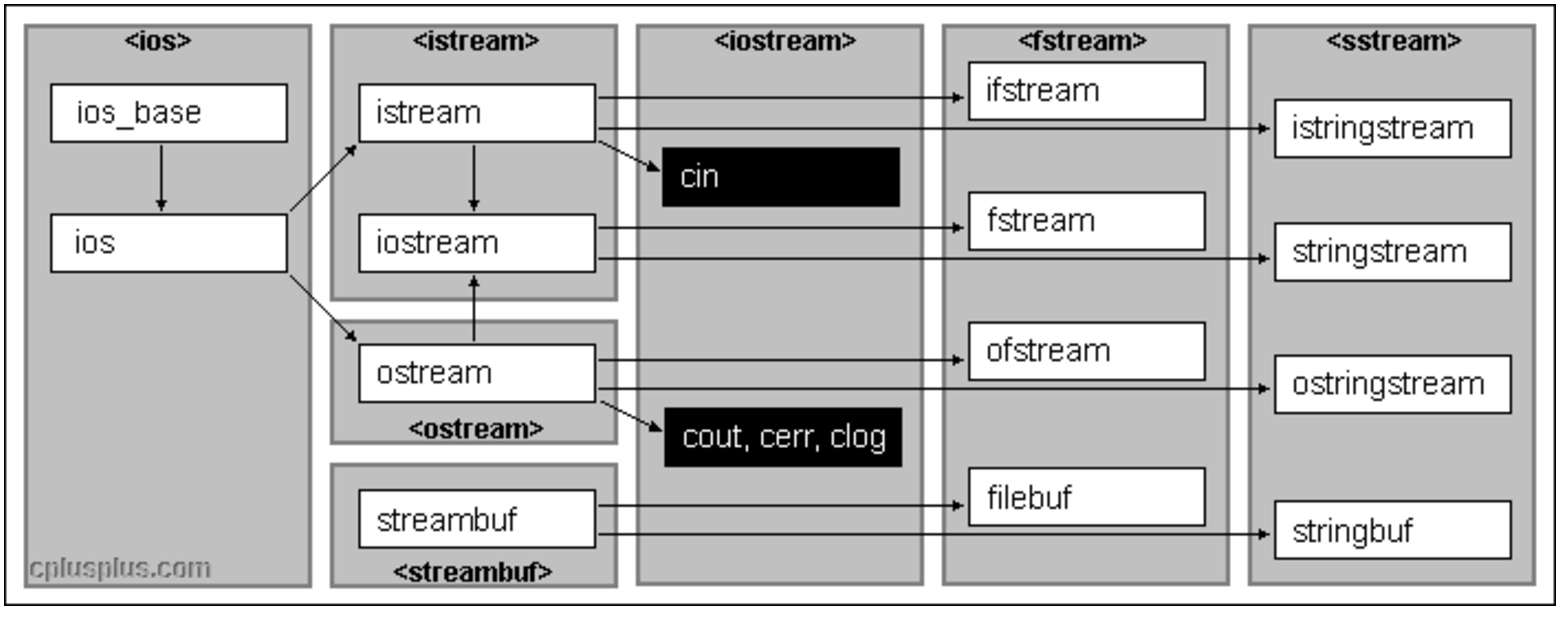
\includegraphics[scale=0.5]{pics/io.png}
	\end{center}
	
	\begin{enumerate}
		
		\item \textbf{iofs} stand for three header files <iostream> <fstream> and <sstream>. <iostream> includes <ios> automatically. They are three main header file you should includes in your C++ application.
		
		\item three classes: \texttt{iostream(streambuf)}, \texttt{fstream(filebuf)}, \texttt{stringstream(stringbuf)} and four pre-defined object: \texttt{cin, cout, clog and cerr} 
		
		\item \texttt{clog} is just like \texttt{cerr}, but it buffer it output.
		
		\item C++ normally flushes the input buffer when you press enter. For output to the display, C++ program normally flushes the output buffer when you transmit a newline character, or reaches an input statement.
		
		\item \verb=>>= and \verb=<<= don't need to format string,  C++ will automatically convert it, it's better than \texttt{printf} and \texttt{scanf} in C language.
		
		\item through inheritance, \texttt{fstream} and \texttt{cin(cout)} has the same interface. \textbf{All the knowledge of \texttt{cin} can be used directly for \texttt{fstream}.} I like this feature the most.
	\end{enumerate}
	
	\item \texttt{peek} return the next character from input stream without extracting from the input stream. For example, you want to read input up to the first newline or period. In this way, I will not read '.' or newline symbol into the \texttt{input}.
\begin{lstlisting}[numbers=none]
char input[80];
int i = 0;
while( (ch=cin.peek()) != '.' && ch != '\n')
cin.get(input[i++];)
input[i] = '\0';	
\end{lstlisting}	
	
	\item \texttt{gcount()} method returns the number of characters read by the last unformatted extraction method. That means character read by the a \texttt{get()}, \texttt{getline()}, \texttt{ignore()}, or \texttt{read()}, but not extraction operator. \texttt{putback()} function inserts a character back in the input buffer.
\end{itemize}



\section{Input/output stream in C++}

\subsection{Input basic knowledge}

\begin{itemize}
	\item For input stream, you need to master \textbf{One basic idea, Two languages, Three data type.}
	\item \textbf{One basic idea:} To make continuous input, you need to use \texttt{while(inputMethod)}. Two things can happen in this process:
	\begin{enumerate}
		\item The user wants to end input(e.g., by pressing ctrl+D) or read to the end of file.
		\item Reading fails (e.g.,  when using \texttt{cin>> int}, but inputting the letter 'a').
	\end{enumerate}
	
	In the previous two conditions, \texttt{inputMethod} will return false. To distinguish between \texttt{EOF} or \texttt{error} inside the while loop, you need to use some flag or status. Alternatively, you can skip the input while loop entirely.
	
	\item \textbf{Two languages:} For c and c++, they use the different inputMethods functions or objects. 
	
	\item \textbf{three data types:} They are: 1)character(white space) 2)number and word(no space in middle), and 3)string(include space in middle)
	
	\begin{tabular}{|p{0.05\textwidth}|p{0.25\textwidth}|p{0.3\textwidth}|p{0.3\textwidth}|}
		\tophline
		& Number and non-white  character word & Character (including white characters) & string(line)\\
		\tophline
		C &\texttt{scanf("\%d \%f \%c \%s",\&i, \&f,\&c);}  & \texttt{int a = getchar();} & \texttt{fgets(char*p, n, stdin)} \\
		\tophline
		C++ & \verb|cin>>i>>f>>c>>w;| & \texttt{cin.get(char \& c);} \newline  \texttt{Ch = cin.get();} & \texttt{cin.get( char *p, n);} \newline \texttt{cin.getline(char *p, n)}; \newline \texttt{getline(cin, string)};
		\bottomhline
	\end{tabular}
	
	
	\item When you use \texttt{scanf} function, you need to specify exact data type when you read.
	\begin{enumerate}
		\item h:  \texttt{short int} or \texttt{short unsigned}. Example: \texttt{\%hd} or \texttt{\%hu}.
		
		\item l:  a \texttt{long int} or \texttt{long unsigned}, or double (for \%f conversions.) Example: \texttt{\%ld, \%lu,} or \texttt{\%lf}.
		
		\item L: The value to be parsed is a \texttt{long long} for integer types or \texttt{long double} for float types. Example: \texttt{\%Ld, \%Lu,} or \texttt{\%Lf}.
		
		\item *: Tells scanf() do to the conversion specified, but not store it anywhere. This is what you use if you want \texttt{scanf()} to eat some data but you don't want to store it anywhere; you don't give scanf() an argument for this conversion. Example: \texttt{\%*d}.
	\end{enumerate}
	
	
	\item \texttt{scanf("\%c" \&c)} will read any character, including whitespace character. If you want to scanf skip any whitespace, you can use space before \texttt{\%c}.
	
\begin{lstlisting}[frame=single, language=c++, mathescape=true]
while(true){
	scanf("%c",&c);
	//scanf(" %c",&c);
	printf("you input: %d" c);
}
//When you input "a(enter)", output will be:
//you input: 97('a' ascii code)
//you input: 10('enter' ascii code)	
\end{lstlisting}		
	
	\item \verb=cin>>c= will not read(just skip) white characters(tab, space , newline), If you want to read them from input buffer, You should use \texttt{getchar()} or \texttt{cin.get()}; 
	\begin{lstlisting}
		while(true){
			cin>>c;
			cout<<"you input:"<<c<<endl;
		}
		//When you input  "    a(enter)" output will be:
		//you input: a, then cursor wait here, skip enter and space.
	\end{lstlisting}
	
	\item If you want the user to input his or her name(including first name and last name), using \verb=cin>>= or \texttt{scanf} will terminate the string after it reads the first space. The best way to handle this situation is to use the function to read a line;
	
\begin{lstlisting}[frame=single, language=c++]
scanf(%s,char_array) //c, read a word until white character. not read newline
cin>>char_array  //c++, or
cin>> str;

gets(char_array)  //c read a line	
fgets(char_array, n , FILE *) //recommend to use this for safety.

cin.getline(char * ,int n) // c++ read and discard newline
cin.get(char * ,int n)  
std::getline(istream&  is, string& str)	
\end{lstlisting}	
	
	\item \texttt{cin.read} function has the same interface with \texttt{cin.get}, but it doesn't append a null character to input, It's not intend for keyboard input, but for binary format of file.
	
	\item Regarding input using \texttt{cin}, please remember the following mnemonic:, three \texttt{get}, two \texttt{getline}, other use \texttt{operator >>}. The interface of these functions are below:
\begin{lstlisting}[frame=single, language=c++]
int iostream::get();      //three get functions
istream& iostream::get (char& c);
istream& iostream::get (char* s, streamsize n, char delim);

istream& iostream::getline (char* s, streamsize n, char delim ); //two getline
istream& getline (istream&  is, string& str, char delim);	
	
\end{lstlisting}	
	
	\item Difference between \texttt{cin.get(char)} and \texttt{int = cin.get()}.
\begin{lstlisting}[frame=single, language=c++]
while(cin.get(c)) // use cin.get(char) in reading loop

cin.get() != '\n' //use cin.get() return character to test sth.	
cin.get()!= EOF //cin.get() return int to compare with EOF	
\end{lstlisting}	
	\begin{description}
		\item[Line 4:] Use int to compare with EOF, because EOF may not be expressed by char type.
	\end{description}
	
	\item Three confused functions to read line: \texttt{cin.get} and \texttt{cin.getline} are almost the same thing.
\begin{lstlisting}[numbers=none]
cin.get ( char* s, streamsize n, char delim ); //don't discard delimiters
cin.getline (char* s, streamsize n, char delim );
istream& getline (istream&  is, string& str); //easy to use.
\end{lstlisting}
	
	\begin{enumerate}
		
		\item If you don't know the maximum length of each line, you can use \texttt{getline(cin, string)} and don't need to input any length (although you can reserve the length of the string if you want to avoid allocating memory). If you want to read a line into a string, avoid using \texttt{cin.getline} because it only reads into a character array.
		
		\item \texttt{cin.get()} doesn't discard delimiters from the input stream. However, \texttt{cin.getline()} will read and discard the newline character. This is easy to remember because a \textbf{line} is defined by a newline character.
		
		\item In \texttt{cin.getline(char* s, int n)}, The failbit flag is set if the function extracts no characters(newline is a character), Or if the delimiting character is not found once (n-1) characters have already been written to s. Note that if the character that follows those (n-1) characters in the input sequence is precisely the delimiting character, it is also extracted and the failbit flag is not set. In \texttt{cin.get(char* s ,  int n)}. The failbit flag is set only if the function extracts no characters.
		
		\item If you are talking about the newline character from a console input, it makes perfectly sense to discard it, So use \texttt{cin.getline()}. Or you don't want to customized flexible reading method, just read a line from a file, please use \texttt{cin.getline()}.
		
		\item \texttt{cin.get(char* s, n)} is more flexible than \texttt{cin.getline}. Because when it read to the array is full, It doesn't set failbit. At this time you can use \texttt{gcount()} or \texttt{peek()} to see if next character is new line. It's more customized than \texttt{cin.getline()};
		
		\item The above rules may look complicated, but if you understand them from a semantic perspective, it will be easier to comprehend. The \texttt{cin.getline} function is designed to read a line, so it has specific rules for handling newlines. On the other hand, \texttt{cin.get(char*p, n)} is simply a version of \texttt{cin.get(char)} that reads multiple characters.
	\end{enumerate}
	
\end{itemize}

\subsection{Input error}

\begin{itemize}
	\item To handle input errors, keep in mind that in C, the functions typically return either EOF or NULL, whereas in C++, they generally return false.
	
	\begin{center}
		\begin{tabular}{|c|c|c|c|}
			\tophline
			& Number, non-white & character, white  & string \\
			\tophline
			C & scanf return EOF & getchar return EOF & fgets return NULL \\
			\tophline
			c++ & cin return false & cin return false & cin.getline return false \bottomhline
		\end{tabular}
	\end{center}
	
	\item When you can't continue to read from input stream, you need to know if it's end of file or fail. In C language, you can use \texttt{feof} and \texttt{ferror} function, in C++, you can use \texttt{cin.eof()}, \texttt{cin.fail()} or \texttt{cin.bad()} three functions. \texttt{cin.bad()} means serious system error happens, and input buffer can't be consistent and can't recovery anymore. When \texttt{failbit} or \texttt{badbit} are set, \texttt{cin.fail()} returns true, so you need to judge it by \texttt{bad()} again if this information is important for you. Usually, \texttt{bad()} is not used very often.
	
	\item The \texttt{eofbit} is an interesting topic. When you reach the logical end-of-file (but have not yet read it), the \texttt{eofbit} will not be set. Instead, it's set by a read function and not by position. To check for the logical end-of-file, you can use the \texttt{std::ifstream::peek()} function. In other words, the \texttt{eofbit} is set by the last read EOF position. When you read the EOF position, both the \texttt{failbit} and the \texttt{eofbit} are set. So if the \texttt{EOF} is set, the \texttt{failbit} must also be set. If only the \texttt{failbit} is set, it means that an input error has occurred. In either of these two conditions, the \texttt{istream} will return \texttt{false} by the \texttt{operator bool}.
	
	%	\item In http://en.cppreference.com/w/cpp/io/basic\_ios/operator\_bool . You can see eofbit are true and failbit are false, operator bool return true. I don't' know when it will happen. \textbf{ eof() function returns "true" after the program attempts to read past the end of the file.}  But when read action set eofbit, it will set failbit at the sametime, so bool operator will return false because failbit are set.
	
	
	\item You can use \texttt{clear()} and \texttt{setstate()} to set the states. Why? It depends on what the program is trying to accomplish. They provide a means for you to change the state of the input stream. \texttt{setstate()} is different from \texttt{clear()}: \texttt{clear()} clears all the status bits, but \texttt{setstate()} sets specific bits. For end-users, we don't use it very often, we just use \texttt{clear()} more.
	
	\item You can use\texttt{ ios::exceptions()} method to control if exceptions will be thrown, when the eofbit, failbit and badbit is set.
\begin{lstlisting}[frame=single, language=c++]
std::ifstream file;
file.exceptions ( std::ifstream::failbit | std::ifstream::badbit );
try {
	file.open ("test.txt");
}
catch (std::ifstream::failure e) {
	std::cerr << "Exception opening/reading/closing file\n";
}			
\end{lstlisting}
	
	
	\item For \texttt{rdstate()}, it will return all the bit values. You can use the bitwise operator \& to check if a specific bit (such as the \texttt{failbit}) has been set. However, in practice, you can just use \texttt{fail()} directly. Therefore, we don't use this function very often.
\begin{lstlisting}[frame=single, language=c++]
std::ifstream is;
is.open ("test.txt");
if ( (is.rdstate() & std::ifstream::failbit ) != 0 )
std::cerr << "Error opening 'test.txt'\n";	
\end{lstlisting}	
	
	
	\item The \texttt{clear()} function is very important. When \texttt{cin.fail()} returns \texttt{true}, you have to use \texttt{clear()}. Otherwise, all subsequent \texttt{cin} operations will not work. For example, when you input "12345Enter", line 2 \texttt{cin.getline(str, 5)} will only read "1234" characters(4=5-1),and set the \texttt{failbit} to \texttt{true}. If you don't clear the failbit, the \texttt{cin>>ch} in line 6 will not read any character. 
	
\begin{lstlisting}[]
char ch, str[20];
cin.getline(str, 5); 
cout<<"flag1:"<<cin.good()<<endl;    // check good bit
cin.clear();   //without, cin>>ch below will not work at all
cout<<"flag1:"<<cin.good()<<endl;    // check good bit again
cin>>ch;
cout<<"str:"<<str<< " ch:" <<ch<<endl;
//output is below:
flag1:0 // good()return false
flag2:1 // good()return true after clear().
str:1234 ch:5	
\end{lstlisting}	
	
\end{itemize}

\subsection{Input Pattern}

\begin{itemize}
	\item "It is a \texttt{BAD} idea to test the stream in the loop condition check and then read or write to it inside the body of the loop statement. This is because the act of reading may make the stream bad. It is usually better to do the read as part of the test.
	
\begin{lstlisting}[numbers=none]
while(!cin.fail()){  // that is bad programming style
	cin>>i;  //here may make stream fail().
	.....      //then i is not valid value
}	
\end{lstlisting}	
	
	\item If you just want to input, You don't want to know eof or deal with failbit. You can use below pattern: test and read at the same time. 
	
\begin{lstlisting}[numbers=none]
while(scanf("%d",&i) != 1) //in c language, use these to exit loop!
while((int c = getchar())!=EOF)
while( fgets(line, sizeof(line), fp) != NULL )

while(cin>>input)  //in C++ language, use bool operator to exit loop.
while(cin.get(p, 20) )
while(getline(ifstream, string))	
\end{lstlisting}	
	
	\item If you want to know if you've reached the end of the file or if you need to handle errors, you can use the code below. When you press enter, the read operation will end. When you input a letter, it will discard these letters until you input a number.
\begin{lstlisting}[frame=single, language=c++]
While(true)  {
	cin>>x;// or getline(ifstream, string);
	if(cin.eof()){   //If it's EOF
		... //take action
	}	
	if(cin.fail()){    //deal with Invalide input
		cin.clear(); //Important. clear state and buffer
		while(cin.get()!='\n')  //get rid rest of line,
		continue ;          //including '\n'
		continue;
	}
	...  // input is right. Do some useful things.
}	
\end{lstlisting}	
	
	\item In the previous example, Why do we need to distinguish eof and fail? When fail happen, maybe there are invalid character in buffer. After clean the buffer, I can continue to read input from input buffer. Three methods to clean invalid character in the buffer.
\begin{lstlisting}[numbers=none]
cin.clear();    //Important. clear state and buffer
while(cin.get()!='\n')
continue ;      // method 1

while(!isspace(cin.get()))
continue;  //method 2

basic_istream& ignore(streamsize _Count = 1, \
int_type _Delim = traits_type::eof());  //method 3
cin.ignore(5, 'a');
cin.ignore(numeric_limits<streamsize>::max(), '\n');	
\end{lstlisting}	
	
	\item You can use \texttt{istream\_iterator} instead of a while loop. Details on how to use it can be found in the iterator section of the STL chapter. 
	
	%\begin{lstlisting}[frame=single, language=c++]
	%class A{
		%private:
		%	int x,y;
		%	friend istream& operator>>(istream& in, A&);
		%	friend ostream& operator<<(ostream& in, const A&);
		%};	
	%istream& operator>>(istream& in, A& a){
		%	in>>a.x>>a.y;
		%	return in;
		%}	
	%ostream& operator<<(ostream& out, const A& a){
		%	out<<a.x<< " " <<a.y;
		%	return out;
		%}
	%	
	%vector<A> v;
	%copy(istream_iterator<A>(cin), istream_iterator<A>(), back_inserter(v));
	%copy(v.begin(), v.end(),ostream_iterator<A>(cout, "\n"));
	%\end{lstlisting}
	
	\item In summary, it is better to use a conditional statement to exit the loop. If you need to take specific actions to handle end-of-file or errors, use a \texttt{while(true)} loop and then use \texttt{eof()}, \texttt{fail()}, \texttt{clear()}, or \texttt{feof()} functions in C++ or C to handle and break the loop.
	
	\item how to read csv file. you need to use locale object. 
\begin{lstlisting}[frame=single, language=c++]	
struct Trade {
	long long time;
	string name;
	int quantity;
	int price;
	friend fstream& operator >> (fstream& in, Trade& t);
};
fstream& operator >> (fstream& in, Trade& t) {
	in >> t.time>> t.name>>t.quantity>>t.price;
	return in;
}

struct csv_whitespace : std::ctype<char> {
	static const mask* make_table() { // make a copy of the "C" locale table
		static std::vector<mask> v(classic_table(), classic_table() + table_size);
		v[','] |= space;  // comma will be classified as whitespace
		return &v[0];
	}
	csv_whitespace(std::size_t refs = 0) : ctype(make_table(), false, refs) {}
};

fstream fin("C://C++//input.csv", ios_base::in);
fin.imbue(locale(cin.getloc(), new csv_whitespace));
Trade t;
while (fin >> t) {
	cout << t.name << endl;
	cout << t.time << endl;
}			
\end{lstlisting}		
	
\end{itemize}

\subsection{Output stream}

\begin{itemize}
	\item For \texttt{cout}, it can recognize the data type automatically, and it is extensible. You can redefine the \verb=<<= operator so that \texttt{cout} can recognize your data type.
\begin{lstlisting}[frame=single, language=c++]
class Foo{
	friend ostream & operator<<(ostream& s,const Foo &r);
}
ostream & operator<<(ostream& s, const Foo &r){
	s<<Foo.a<<Foo.b<<endl;
	return s;
}	
\end{lstlisting}	
	
	\item Only use std::endl if you absolutely need to make sure that some output needs to materialize immediately. Each call to std::endl flushes the output buffer and writes the output immediately. This can lead to serious performance degradation, if done frequently.
	
\begin{lstlisting}
std::cout << "some text" << std::endl;
std::cout << "more text" << std::endl; //bad

std::cout << "some text\nmore text\n"; //good	 
\end{lstlisting}	
	
	\item  How to print pointer address in C and C++?
\begin{lstlisting}[numbers=none]
char* amount = "dozen";
cout<< amount  ; //print "dozen" string	
cout<<(void*) amount;//prints the address of pointer
printf("%p", (void*) p);
\end{lstlisting}		
	
	\item Formatting is a key point for output. You need to know the common manipulators that allow you to control the output format. These include number base manipulators such as \texttt{hex}, \texttt{oct}, and \texttt{dec}, as well as field width manipulators such as \texttt{width}, \texttt{fill}, and \texttt{precision}. You can use the \texttt{setf()} function to set these manipulators.
\begin{lstlisting}[]
ios state(nullptr);
cout << "The answer in decimal is: " << 42 << endl;
state.copyfmt(cout); // save current formatting
cout << "In hex: 0x" // now load up a bunch of formatting modifiers
<< hex << uppercase << setw(8) << setfill('0')<< 42<<endl; 
cout.copyfmt(state); // restore previous formatting	
\end{lstlisting}	
	
	\item You don't need to know the details, just name of them. When you want to use them go to reference website to look.  You need to include \texttt{<iomanip>}. Another reason that I don't introduce more detail here is that there is a better solution in C++ 20, that is \texttt{std::format.}  I introduce this in the last chapter--Modern C++. 
	
	\item \verb=<<= is a bitwise left-shift operator in C language, but in C++, we overloaded it in ostream class, cout is a object of ostream.  You can use \verb=cout<<flush= to force flushing the output buffer
	
	\item \texttt{cout.write} can be used to output a string, It will output certain length string, even reach the end of string.
\end{itemize}

\subsection{file stream and string stream}


\begin{itemize}
	\item When you have a good understanding of cin and cout, you will find that file operations are also quite simple. You just need to replace cin or cout with the appropriate ifstream, ofstream, or fstream object. They share the same interface and usage. That's the one of advantages of OOP.
	
\begin{lstlisting}[numbers=none]
std::fstream ifs;
ifs.open ("test.txt", ios_base::in| ios_base::binary);
if(!ifs.is_open())
exit(1);
char c = ifs.get(); // use all previous input methods
ifs.close(); //Due to RAII, you can skip this statement.	
\end{lstlisting}	
	\item Only read ifsteam;  Only write ofsteam;  write and read fstream.  For \texttt{ios\_base::binary} mode, use write() and read() funciton. For writing, pay attention to the difference between \texttt{ios\_base::trunc} and \texttt{ios\_base::app}
	
	\item Random access is used mostly on binary file. Because the position can be pinpointed exactly. For \texttt{seekg()} for input, and \texttt{seekp()} for output. (\texttt{p} is put, \texttt{g} is get) It moves the pointer. \texttt{tellp()} and \texttt{tellg()} functions tell the position of the pointer.
	
	
	\item You can build a stringstream from a string or convert a stringstream back to a string. The stringstream is a convenient way to manipulate strings like an independent I/O device. It is often useful to use stringstream to convert between strings and numerical types. The usage of stringstream is similar to iostream, so it is not difficult to learn. The stringstream class is used for inserting and extracting data to/from string objects, acting as a stream for the string object. It is similar to cin and cout streams except that it doesn't have an input/output channel.
	
\begin{lstlisting}[frame=single, language=c++]
char sentence []="Yan is 41 years old"; //C language method
char str [20];
int i;
sscanf (sentence,"%s %*s %d", str, &i);
sprintf(.....);

stringstream outstr;  //C++ method, change number to text
outstr<<"salary value"<<123333.00<<endl;
string str = outstr.str() 

istringstream Instr(str); //20 change text to number  
while(instr>>number)     //str is "123 456 789"
cout<<number<<endl		
\end{lstlisting}	
	
	
	
	\item Counting the number of words in a string.
\begin{lstlisting}[frame=single, language=c++]
string str = "Simple Questions To Check Your Software Testing Basic Knowledge"; 
stringstream s(str);  
string word; int count = 0;
while (s >> word)// here s is just like cin 
count++;	
\end{lstlisting}	
	
	\item We usually use stringstring to finish token task.
\begin{lstlisting}[]
string P, K;
getline(cin, P); //input "yan.x.zhao"
stringstream N(P); //build a stringstream,
while (getline(N, K, '.')) { //geline support input delim
	cout << K << endl; //output yan x zhao
}	
\end{lstlisting}	
\end{itemize}





\chapter{Initialization}
\section{Basic knowledge}

\subsection{Basic principles and terminology}
\begin{itemize}
	\item Always initialize variables before using them, and manually initialize any non-member objects of built-in types, including pointers.
	
	\item There are three names you need to distinguish: 1) initializer list, 2) braces (uniform) initialization, and 3) member initialization list (mem-init).

	\begin{enumerate}
		\item The member initialization list is used in C++ constructors to initialize all members inside an object. It offers several advantages, as detailed in the 'OOP' chapter. For example, reference type member variables can only be initialized by the member initialization list. Additionally, it provides higher efficiency as the copy constructor is only called once."
		
		\item Braces initialization is a generic initialization syntax(method), it supports a kind of uniform initialization, such as class member and aggregation. At the same time, it avoids narrowing and vexing parsing problem. 
		
		\item Initializer list is \texttt{std::initializer\_list}. It is a \textbf{new data type. just like std::list.}
	\end{enumerate}

	\item A constructor with one parameter is called a converting constructor in C++. After C++11, any constructor that is not declared with the specifier 'explicit' is also considered a converting constructor. This includes both implicitly-declared and user-defined non-explicit copy constructors and move constructors.
	
	\item Constructors with more than one parameter are also considered converting constructors in C++11. This is because the new standard provides a convenient syntax for passing arguments and returning values using braced-init-lists. Consider the following example: The ability to specify the return value as a braced-init-list is considered to be a conversion. This uses the converting constructor for foo that takes a float and an int. In addition, we can call this function by doing bar(\{2.5f, 10\}).
\begin{lstlisting}[numbers=none]
struct Foo{
	Foo() { }         // converting constructor (since C++11)  
	Foo(int) { }      // converting constructor
	Foo(float, int) { } // converting constructor (since C++11)
};
Foo bar(Foo f) {
	return {1.0f, 5}; //CONVERTING two numbers into Foo.
}	
\end{lstlisting}	

	
	\item It's important to note that whether a constructor is a converting constructor only depends on whether it has the \texttt{explicit} specifier. If there is no \texttt{explicit} specifier, even constructors with zero or more than one parameter are considered converting constructors."
	
	\item List(brace) initialization(syntax description) is also called uniform initialization(semantic description), In this book, uniform, list(brace) initialization are interchangeable. In syntax level, it uses braced-init-lists (\{\}) to enclose initializer values.
	
	\item List initialization is a feature that permits the usage of a consistent syntax to initialize variables and objects which are ranging from primitive type to aggregates. although the syntax is uniform, but for differnt T type, it carry out different actions, such as carry out value initialization or call converting constructor. 
	
	\item List initialization is comprised of direct-list-initialization and copy-list-initialization. 
	
	\item default constructor is different with default initialization. copy constructor is also different with copy initialization.
	
	\item A good reference page is \verb|https://en.cppreference.com/w/cpp/language/initialization|. Anytime you have question, you can go to there to get the official explanation. 
\end{itemize}

\subsection{static initialization and dynamic initialization}
\begin{itemize}
	\item In the same translation unit, formally, C++ initializes static and global variables in this order:
	\begin{enumerate}
		\item Static initialization.
			\begin{enumerate}
			\item Zero initialization.
			\item Const initialization.
			\end{enumerate}
		\item Dynamic initialization.
	\end{enumerate}
		
\begin{lstlisting}[numbers=none]
int g0;  //zero initialization
int g1 = 42;    //  constant initialization
extern int f();
int g2 = f();   //  dynamic initialization
\end{lstlisting}

	\item You can see the dynamic initialization happen after static initialization. Sometimes it causes some subtle bugs shown below:
\begin{lstlisting}[frame=single, language=c++, mathescape=true]
int a = f(); // call f here
int x = 22; // but this line is executed first.
int f() {
	++x;
	return x; 
} //x equals to 23, not 22. because static init is earlier than dynamic
\end{lstlisting}

	
	\item Pay attention to the order of initialization for global objects. While the order can be specified within a single translation unit, it is not guaranteed to be the same between translation units (see Effective C++ Item 47). This uncertainty in initialization order between separate translation units can cause problems, as described below.
	
\begin{lstlisting}[frame=single, language=c++]
#include "x.h" // File x.cpp
X x;    //x maybe initialize before y or after y.
	
#include "y.h" // File y.cpp
extern X x;
Y y;
Y::Y(){ 
	x.goBowling(); //Here x maybe not be constructed
}
\end{lstlisting}
	
	\item  There are two ways to resolve this issue. First, we do not encourage the use of global objects unless they are absolutely necessary. Second, you can use the Singleton design pattern.
	\begin{lstlisting}[numbers=none]
#include "x.h"  // File x.cpp
X& getX(){
	static X x;   //static X* px = new X();
	return x;     //return *px
}
	
#include "y.h" // File y.cpp
Y y;
Y::Y(){
	getX().goBowling();
}
\end{lstlisting}
\end{itemize}


\subsection{Initialization  categories}

\subsubsection{Six kinds of initialization}
\begin{itemize}
	\item There are six \textbf{initialization methods} in C++:
	\begin{enumerate}
		\item There are two points to clarify regarding default initialization syntax and its use. First, default initialization does not necessarily call the default constructor. Second, default initialization does not necessarily set the variable to zero. Rather, default initialization calls the default constructor if one exists, or does nothing if there is no default constructor. In the latter case, the result is an indeterminate value. Here is an example of default initialization:
\begin{lstlisting}[numbers=none]
T t;
new T;  //default
\end{lstlisting}

	
\begin{lstlisting}
struct T1 { int mem; };
struct T2{
	int mem;
	T2() { } // "mem" is not in the initializer list
};
int n; // static non-class, a two-phase initialization is done:
	// first, zero initialization, then default initialization does nothing
	
int main(){
	int n;          // non-class, the value is indeterminate
	std::string s;  // class, calls default constructor, s is "" (empty string)
	std::string a[2]; // array, default-initializes the elements, a is {"", ""}
	//  int& r;       // error: a reference
	//  const int n;  // error: a const non-class
	//  const T1 t1;  // error: const class with implicit default constructor
	T1 t1;            // class, calls implicit default constructor
	const T2 t2;   // const class, calls the user-provided default constructor
                  // t2.mem is default-initialized (to indeterminate value)
}
\end{lstlisting}

\begin{description}
	\item[Line 8:] static initialization and default initialization is not exclusive each other, they can be combined. 
\end{description}


	\item Value initialization syntax and example.
\begin{lstlisting}[numbers=none]
T(); T{};
new T(); new T{};
Class::Class(...): member(), member{} {...} 
// class member initializer lists (value Init)
\end{lstlisting}


\begin{lstlisting}
struct T1{
	int mem1;
	std::string mem2;
}; // implicit default constructor

struct T2{
	int mem1;
	std::string mem2;
	T2(const T2&) { } // user-provided copy constructor, no default ctor
};

struct T3{
	int mem1;
	std::string mem2;
	T3() { } // user-provided default constructor
};
std::string s{}; // class => default-initialization, the value is ""

int n{};                // scalar => zero-initialization, the value is 0
double f = double();    // scalar => zero-initialization, the value is 0.0
int* a = new int[10](); // array => value-initialization of each element 0

T1 t1{};		// class with implicit default constructor =>
// t1.mem1 is zero-initialized 0, t1.mem2 is default-initialized ""
//  T2 t2{};	// error: class with no default constructor

T3 t3{};		// class with user-provided default constructor =>
// t3.mem1 is default-init to indeterminate, t3.mem2 is default-init ""

std::vector<int> v(3);  // value-initialization of each element to 0
\end{lstlisting}

		\item Direct initialization syntax and example.
\begin{lstlisting}[numbers=none]
T object(arg, ... );
T(arg1, arg2, ... );
new T(args, ...)
: member(args, ...)   // class member initializer lists
T(other)              // function-style cast
static_cast<T>(other) // explicit static_cast
[arg](){...}          // lambda closure arguments captured by value
\end{lstlisting}


\begin{lstlisting}[numbers=none]
struct Foo {
	int mem;
	explicit Foo(int n) : mem(n) {}
};

Foo f(2); // f is direct-initialized:
Foo f2 = 2; //error, because constructor is explicit.
\end{lstlisting}


		\item Copy initialization syntax and example.
\begin{lstlisting}[numbers=none]
T object = other;     // Initialization via assignment
T array[N] = {other}; // In array-initialization, the individual value are copy-init
f(other)                 // Pass-by-value
return other;            // Return-by-value
catch (T object)         // Catch-by-value
throw object;
\end{lstlisting}

\begin{lstlisting}[]
struct A {
	operator int() { return 12;}
};

struct B {
	B(int) {}
};

int c = b; // this is also copy initialization. 
A a;
//B b1 = a;  // it's copy initialization, but fail. 
B b2{a};     // calling A::operator int(), then B::B(int)
B b3 = {a};  //like line 12. not copy initialization, is list initialization
auto b4 = B{a}; //like line 12. not copy initialization, but direct init.
\end{lstlisting}

		\item Aggregate initialization is used when initializing arrays or simple struct (all-member-public, no user-provided c'ctors.)
\begin{lstlisting}[numbers=none]
T object = {arg1, arg2, ...}; // If T is an array or a simple struct
T object{arg1, arg2, ...};    // If T is an array or a simple struct
\end{lstlisting}

\begin{lstlisting}[numbers=none]
struct S {
	int x;
	struct Foo {
		int i;
		int j;
		int a[3];
	} b;
};

S s1 = { 1, { 2, 3, {4, 5, 6} } };
S s2 = { 1, 2, 3, 4, 5, 6}; // same, but with brace elision
S s3{1, {2, 3, {4, 5, 6} } }; // using direct-list-initialization syntax
S s4{1, 2, 3, 4, 5, 6}; // error until CWG 1270: 
						// brace elision only allowed with equals sign
\end{lstlisting}

		\item reference initialization. It must has a reference symbol.
\begin{lstlisting}[numbers=none]
T & ref = object ;
T & ref = { arg1, arg2, ... };
T & ref ( object ) ;
T & ref { arg1, arg2, ... } ;
\end{lstlisting}
	\end{enumerate}

    \item You can use brace elision in the aggregate initialization.
\begin{lstlisting}
struct A{
	int foo;
	double bar;
};
struct Aarray{
	A data[2];  //data is an internal array
};
int main() {
	array<int, 5> a{1,2,3,4,5};  // without =, no nested aggregated, brace elision is also ok.
	
	Aarray a1 {
		{  //<--this tells the compiler that initialization of `data` starts
			{ //<-- initialization of `data[0]` starts
				0, 0.1
			}, //<-- initialization of `data[0]` ends
			
			{2, 3.4}  //initialization of data[1] starts and ends, as above
		} //<--this tells the compiler that initialization of `data` ends
	};

	Aarray a2 = {0, 0.1, 2, 3.4}; //you can use brace elision
	Aarray a3{0, 0.1, 2, 3.4}; //After c++ 14, you don't need =
	Aarray a4{ {0, 0.1}, {2, 3.4} }; //error, this is too many initializers error
}
\end{lstlisting}
\begin{description}
	\item[Line 11:] If you don't want to use brace elision, you have to tell where the initialization begin by adding extra \{\}.
	\item[Line 23:] Without extra \{\}, you will have too many initializers error.
\end{description}

		\item \texttt{std::array} doesn't have any constructors, so it is an aggregate type. Both \texttt{S1} and \texttt{S2} are aggregates, which means we can use brace elision. We recommend using brace elision. Whether you use braces with or without an equal sign, the semantics are the same. However, if an element in the aggregate list is not an aggregate type, you cannot use brace elision. For example, \texttt{S3} is not an aggregate, so you must use correct nested braces.
		 
%		\item  Inside array, it's just another C type array,(\texttt{int a[3]}), so when you use aggregate initialization without brace elision, you have to add extra \{\} to specify it's the boundary of \texttt{int a[3]}. The basic idea is the same as previous code \texttt{struct Aarray}.

\begin{lstlisting}
struct S1 {  //S1 is aggregate type
    S1() = default;
    int x;
    int y;
};
struct S2 { //S2 is aggregate type
    S2() = delete;
    int x;
    int y;
};
struct S3 {
    S3(int x1, int y1) {x = x1; y = y1;}
    int x;
    int y;
};

std::array<S1, 3> a11{1, 2, 3, 4, 5, 6};
std::array<S1, 3> a12={1, 2, 3, 4, 5, 6};
std::array<S2, 3> a21{1, 2, 3, 4, 5, 6};
std::array<S2, 3> a21={ 1, 2, 3, 4, 5, 6};  

std::array<S3, 3> a31{1, 2, 3, 4, 5, 6};// compile fail   
std::array<S3, 3> a31{{{1, 2}, {3, 4}, {5, 6}}};
\end{lstlisting}

    \item Regarding aggregate initialization, more explanation is needed. Here are some points to consider:
    \begin{enumerate}
    	\item Starting from C++14, you don't need to use the assignment operator in brace elision.
    	
    	\item If a member inside the aggregate is also an aggregate, you can simply use brace elision style.
    	
    	\item If a member inside the aggregate is not an aggregate, or you prefer to use nested braces to specify the delimiter, you must add extra braces. For example, consider the \texttt{struct S3} in the previous code.
    \end{enumerate}
    
    
   

	\item Summary of six initialization methods:
\begin{enumerate}
	\item Without parentheses, it indicates to the compiler to use the default initialization.
	
	\item Using empty parentheses or braces initializes the variable with a default value. The compiler uses a user-defined value if one exists, otherwise it sets the value to zero.
	
	\item Using parentheses with a value initializes the variable with the specified value.
	
	\item When passing a variable to a function or returning a variable from a function by value, it's considered copy initialization.
	
	\item Aggregate initialization can only be used for aggregate types.
	
	\item Reference initialization is the simplest form of initialization.
\end{enumerate}

	\item After learning about the six forms of initialization, it's important to understand some key differences. In the next three sections, I'll explain the differences between value initialization and default initialization, direct initialization and copy initialization, and traditional copy initialization and list copy initialization. These concepts can be complicated, but don't worry – a short summary will be provided at the end of each section. Let's get started!
\end{itemize}


\subsubsection{Value initialization and default initialization}
\begin{itemize}
 
	\item Let's take a look at some examples that demonstrate the difference between value initialization and default initialization.
	\begin{enumerate}
		\item Class has a implicit default constructor.
\begin{lstlisting}[frame=single, language=c++]
class Foo{ //implicit default constructor
public:
	int i;
};
const Foo foo; //error, Foo has implicit-default constructor, 
               //just like const int i; trigger error too.
				
Foo foo(); //function declaration, can't use () to call default ctor

Foo foo;     //foo.i is random value
Foo foo1{};	 //foo1.i is zero.		 
\end{lstlisting}

\begin{description}			
\item[Line 10:]	 It's a default init. Standard says: if T is a non-POD (until C++11) class type, then... otherwise, no initialization is performed: the objects with automatic storage duration (and their subobjects) contain indeterminate values. Because Foo is POD class, so default initialization doesn't nothing, leave indeterminate values.

\item[Line 11:]  It's a value init. \texttt{Foo} has a implicitly-defined constructor. Standard says: "if T is a class type with a default constructor that is neither user-provided nor deleted (that is, it may be a class with an implicitly-defined or defaulted default constructor), the object is zero-initialized and then it is default-initialized if it has a non-trivial default constructor;"
\end{description}

		\item Class has a defaulted default constructor.
\begin{lstlisting}[frame=single, language=c++]
class Foo{ //implicit default constructor
public:
	Foo() = default;
	Foo(const Foo&){...};
	int i;
};
	
const Foo foo; //error too.
	
Foo foo;     //foo.i is random value
Foo foo1{};	 //foo1.i is zero.		 
\end{lstlisting}
\begin{description}			
	\item[Line 3:]  How to understand \texttt{"= default"}?. Because class has its own copy constructor, so compiler doesn't produce implicit default ctor. In order to generate one, you should use \texttt{"= default"}.
	
	\item[Line 10:] It's a defaulted default constructor.  Standard says: if T is a non-POD (until C++11) class type, the constructors are considered and subjected to overload resolution against the empty argument list. The constructor selected (which is one of the default constructors) is called to provide the initial value for the new object;
	
	\item[Line 11:] It's a value init. Standard says: "A class with an implicitly-defined or defaulted default constructor, the object is zero-initialized."
\end{description}


		\item Class has a user-defined default constructor.
\begin{lstlisting}[frame=single, language=c++]
class Foo{ //implicit default constructor
public:
	Foo();
	int i;
};

Foo::Foo() = default; 
    //it is just like Foo::Foo() {}, it is user defined constructor.
			
const Foo cfoo; //cfoo.i is random value 
			
Foo foo;     //foo.i is random value
Foo foo1{};	 //foo1.i is random value.	
Foo* pf = new Foo;   //just like Foo foo; pf->i is random 
Foo* pf1 = new Foo();  // just like new Foo{}
Foo* pf2 = new Foo{};  // just like Foo foo{};		 
\end{lstlisting}
\begin{description}			
	\item[Source code:] If there is a user-defined constructor, the compiler will call that constructor. If the user-defined constructor does not initialize all the member variables, then the uninitialized member variables will have random values. 
\end{description}

	 \item Value initialization also kick in when you use \texttt{new}. Detail can be found: "Do the parentheses after the type name make a difference with new?"

	\end{enumerate}
		
\item Summary:
\begin{enumerate}
	\item \texttt{Foo foo()} is not initialization call at all, it's a function declaration. 
	
	\item If there is an user-defined default constructor, \texttt{Foo foo;} and \texttt{Foo foo1\{\};} both call user-defined default ctor. If it does nothing, then \texttt{i} is random.
	
	\item If there is an implicitly-defined or defaulted default constructor, \texttt{Foo foo;} and \texttt{Foo foo1\{\};} are different. \texttt{Foo foo1\{\};} perform zero initialization. So \texttt{i} is 0. 
	
	\item The behavior of value initialization depends on whether you have a user-defined constructor. If you don't have one, the compiler performs zero initialization. However, if you have a user-defined constructor, the compiler calls your defined constructor directly instead of performing zero initialization. This is because you have higher priority than the compiler in determining how the object should be initialized.
\end{enumerate}

\end{itemize}



\subsubsection{Copy initialization and direct initialization}
\begin{itemize}

	\item It's important to note that copy initialization is different from copy constructor. When you call the copy constructor directly, it's considered direct initialization. On the other hand, if you use copy initialization, it involves two steps: first, a temporary object is created, and then that temporary object is copied to initialize the new object. During direct initialization, only one constructor is called (determined by overload resolution). These are the theoretical definitions of copy initialization and direct initialization. However, in practice, when compiler optimizations are applied, the details of the initialization process may be hidden or simplified.
	
\begin{lstlisting}[frame=single, language=c++]
ClassTest ct1("ab"); //direct initialization
ClassTest ct2 = "ab"; //copy initialization
ClassTest ct3 = ct1; //copy initialization
ClassTest ct4(ct1); //direct initialization
ClassTest ct5 = ClassTest(); //copy init Class has default constructor
\end{lstlisting}
\begin{description}
	\item[Line 2:] When compiler optimizations are turned on, the behavior of copy initialization may be different than what's described by the theoretical definition. For example, consider the case of initializing an object \texttt{ct2}, if the copy constructor is private, the compiler will stop the compilation. However, if the copy constructor is public, the compiler may optimize the initialization process and call the single-argument constructor directly, bypassing the creation of a temporary object. Even though the single-argument constructor is called directly, this is still considered copy initialization.
	
	\item[Line 3:] For \texttt{ct3}, It's copy initialization. Compiler thinks the \texttt{ct1} has been created, then call copy constructor directly. 
	
	\item[Line 4:] \texttt{ct4} is direct initialization call copy constructor. because in theoretical it's only one step, call a constructor by overload. 
	
\end{description}

	\item Copy initialization and direct initialization has different behavior:
	\begin{enumerate}
		\item The first difference lies in explicit decoration.
\begin{lstlisting}[frame=single, language=c++]
struct foo{
	explicit foo(int);
};

foo f0 (42);  // OK
foo f1 = 42;  // not allowed
\end{lstlisting}

		\item Direct initialization can be thought of as a function call to an overloaded function, where the constructors of T (including explicit ones) act as functions, and x serves as the argument. Overload resolution is used to find the best matching constructor, and implicit conversions are performed as needed. Direct initialization has access to all available constructors and can perform any implicit conversions required to match the argument types.
		
%		\item Copy initialization constructs an implicit conversion sequence: It tries to convert x to an object of type T. (It then may copy over that object into the to-initialized object, so a copy constructor is needed too - but this is not important below) copy initialization can just set up one implicit conversion sequence.
%
%\begin{lstlisting}
%struct B;
%struct A { 
%	operator B() {cout<<"A-o-B,"; return B();}
%};
%struct B { 
%	B() { }
%	B(A const&) { cout <<"A-c-B,"; }
%};
%struct C{
%	operator A() {cout<<"C-o-A,"; return A();}
%};
% 
%A a;
%B b = a;  //OK, print A-o-B
%
%C c;
%B b1(c); //OK, print C-o-A, A-c-B
%B b2 = c; //ERROR
%\end{lstlisting}
%
%\begin{description}
%	\item[Line 14:]  copy initialization will construct a conversion sequence when variable \texttt{a} is not type B or derived from it (which is clearly the case here). So it will look for ways to do the conversion, and will find the following two conversion candidates: 1) \texttt{B(A const\&)} and \texttt{operator B(A\&)}. Because variable \texttt{a} is not \texttt{const}, so operator version wins. 
%	
%	\item[Line 17:] Direct initialization behaves like a function call. it will do any implicit conversion it needs to match up argument types.
%	
%	\item[Line 18:] copy initialization can just set up one implicit conversion sequence. Although there is two steps conversion: C-->A-->B, but there is not one step conversion C-->B. So copy initialization fail here.
%\end{description}
	\end{enumerate}

\item Summary:
\begin{enumerate}
	\item In one word, whether it's copy initialization or direct initialization doesn't depend on whether it calls the copy constructor. On the syntax level, it checks if there is an equal sign, while on the semantic level, it depends on whether (in theory) it has two steps.
	
	\item For explicit constructor, only direct initialization work. It call constructor directly, and do any implicit conversion it needs to match up argument types.
	
	\item For copy init, 1) make sure copy constructor accessible(not private) 2) one the right side of =, just set up one implicit conversion sequence.

    \item Usually, we don't make copy constructor explicit, because it will disable function call and return value. \textbf{We only make one parameter constructor explicit.}
\end{enumerate}

		
    \item a good link is \verb|https://www.cnblogs.com/pluse/p/7088880.html|. A good article is "Is there a difference between copy initialization and direct initialization?"

\end{itemize}

%\subsubsection{explicit}
%\begin{itemize}
	%\item When copy constructor is explicit. I never see any source code with explicit copy ctor, so just for studying purpose. 
%\begin{lstlisting}[frame=single, language=c++]
%class A{
%public:
	%A(int a = 0);
	%explicit A(const A &a){} //EXPLICIT copy constructor
%};
	
%void funcX(A a) {
	%//ERROR, take A by value (implicit copying)
%}
%A funcY(){ 
	%A a;
	%return a; //ERROR, returning A by value(implicit copying)
%}
%A a1 = a; //ERROR, implicit copying of A not allowed
%A a1(a); //OK - EXPLICIT copying allowed
%A a = 1;
%\end{lstlisting}
	%\begin{description}
		%\item[Line 4:] \textbf{Usually, we don't make copy constructor explicit, because it will disable function call and return value.}
		
		%\item[Line 14 and 15:] Difference between \texttt{A a(a1)} and \texttt{A a = a1}.  They are almost same. But When copy constructor is explicit,  \texttt{A a1 = a} will not work, but \texttt{A a1(a)} work.
		
		%\item[Line 16:] \textbf{With explicit copy constructor, A a = 1 still work.But when the copy ctor is private, A a = 1 fail }.Although we don't call copy ctor directly, but we need to make sure it accessible. We don't consider copy ctor's explicit in this case.
	%\end{description}
	
	%\item When parameterized constructor and copy ctor are both explicit.
%\begin{lstlisting}[frame=single, language=c++]
%class A{
%public:
	%explicit A(int k):m_a(k){};
	%explicit A(const A& rhs){m_a = rhs.m_a;};
	%int m_a;
%};
	
%A a=110;// ERROR
%A a(110) //this will work here.
%A a1 = a; // ERROR, because copy constructor is explicit.
%\end{lstlisting}
	%\begin{description}
		%\item[Line 8:] it's copy list init, It will call constructor directly, because \texttt{A(int k)} is explicit, so it fails.
		%\item[Line 9:] Work, satisfy explicit requirement
		%\item[Line 10:] it's copy list init, It will call constructor directly, because \texttt{A(const A\& rhs)} is explicit, so it fails.
	%\end{description}
	
	%\item  When single parameter constructor is explicit. That is the production level source code. 
%\begin{lstlisting}
%class A{
%public:
	%explicit A(int k):m_a(k){};
	%A(const A& rhs){m_a = rhs.m_a;};
	%int m_a;
%};
	
%A a = 1; // fail. 
%A a = {1}  //fail
%A a = A{1}  //work
%A a = A(1)  //work
%\end{lstlisting}
	%\begin{description}
		%\item[Line 3 and 4:] Most of time, Single parameter constructor is explicit, copy ctor is not.
		
		%\item[Line 7 and 8:] With explicit A(int i) constructor, A a = 1 will fail, but A a = A{1} will work.
	%\end{description}


%\item \textbf{Summary:}
%\begin{enumerate}
	%\item The first step is to see the right side of =, if converting constructor is explicit, we have to use A\{1\} to explicit call it. For example: \texttt{A a = A\{1\}} will work. \texttt{A a = 1} will not work. 
	
	%\item The second step is to see when you use brace init. if it has initlizer\_list constructor, it has strong preference. we will talk about it later.
	
	%\item The third step is to see if copy constructor is explicit. if yes, A a = A\{1\} will fail, but A a = \{1\} work.
	
	%\item \textbf{explicit copy constructor only disable A a1=a; but not disable A a1=1; But private copy ctor will disable both.}
	
%\end{enumerate}

%\begin{figure}[h]
	%\centering
	%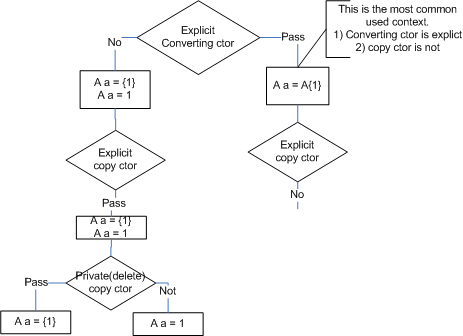
\includegraphics[width=0.8\linewidth]{pics/copy_init.png}
	%\caption{}
	%\label{Explicit and init }
%\end{figure}

%\begin{tabular}{|p{0.27\textwidth}|p{0.6\textwidth}|}
	%\tophline
	%Expression & meaning \\
	%\tophline
	%A a = (i), A a=\{i\} & explicit converting constructor will not work \\
	%\tophline
	%A a = A(i), A a = A\{i\} & explicit copy constructor will not work 
	%\bottomhline
%\end{tabular}


%%\item Last summary about previous three sections.
%%\begin{figure}[h]
%%	\centering
%%	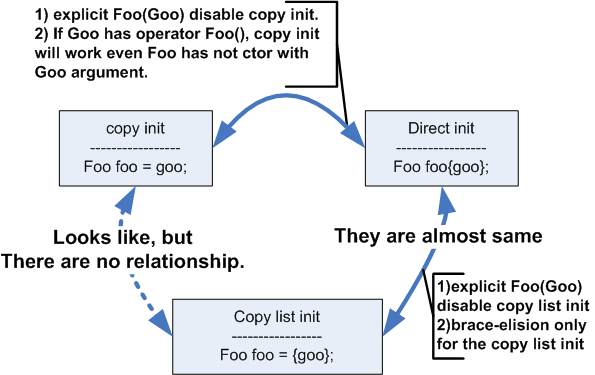
\includegraphics[width=0.9\linewidth]{pics/copy_list.png}
%%	\caption{difference between direct, copy and list-copy init}
%%	\label{fig:copylist}
%%\end{figure}

%\end{itemize}

\section{List initialization}

\subsection{Basic syntax}
\begin{itemize}
		
	\item List initialization is a new syntactic form that can be used with three initialization forms. It is worth noting that value list initialization can also be thought of as value initialization.
	\begin{enumerate}
		\item Value list initialization. It can avoid vexing parsing problem
\begin{lstlisting}[numbers=none]
T object{};
T{};
new T{}
Class { T member{}; };
: member{}  // Class member initializer lists
\end{lstlisting}

		\item Direct list initialization.
\begin{lstlisting}[numbers=none]
T object{arg, ...};
T {arg, ...};
new T{arg, ...}

Class {  // Class member initializer
	T member{arg, ...}; 
};
		
: member{arg, ...} // Class member initializer lists
\end{lstlisting}

		\item Copy list initialization. It has a equal sign in the statement or used in function parameter and return.
\begin{lstlisting}[numbers=none]
T object = {arg, ...};
object = {arg, ...};
Class { T member = {arg, ...}; }; //Class member default initializer
function({arg, ...}); //Initializes temporary for the function arg
return {arg, ...};  //Initializes temporary for return value
\end{lstlisting}
	\end{enumerate}
		
\end{itemize}

\subsection{Traditional copy initialization and list copy initialization}

\begin{itemize}

	\item Here are some basic syntax examples of list copy initialization. One question that often arises is whether the equal sign makes a difference in brace initialization. For example, is there a difference between '\texttt{T a = \{\}}' and '\texttt{T a\{\}}'? The only significant difference that I am aware of is in the treatment of explicit constructors:
	
\begin{lstlisting}
struct foo{
		explicit foo(int);
};
foo f0 {42};    // OK
foo f1 = {42};  // list initiliazation, fail here due to explicit
\end{lstlisting}

	\item Another important difference is a little subtle, can be demonstrated by below code:
	\begin{enumerate}
		\item traditional copy initialization uses notion of user-defined conversion sequences (and, particularly, requires availability of copy constructor, as was mentioned)
		
		\item \texttt{T a = \{\}} is like \texttt{T a\{\}}. So list copy initialization just performs overload resolution among applicable constructors, i.e. list initialization can't use operators of conversion to class type
	\end{enumerate}
\begin{lstlisting}
struct Intermediate {};
struct S{
	operator Intermediate() { return {}; }
};
struct S1{
	S1(Intermediate) {}
};
	
S s;
Intermediate im1 = s; // OK, s-->Intermediate by a user-defined conversion(line 3)
Intermediate im2 = {s}; // ill-formed, just look Intermediate constructor.
S1 s11 = s; // ill-formed 
S1 s12 = {s}; // OK
\end{lstlisting}
	
	\begin{description}
		
		\item[Line 11:] list copy initialization just performs overload resolution among applicable constructors, i.e. List initialization can't use operators of conversion to class type. Intermediate has not constructor with S as argument.
		
		\item[Line 12:] copy initialization can just set up one implicit user-defined conversion sequence. In this case 1) S change to Intermediate by operator, 2) from Intermediate to S1 by constructor.  You can see there are two implicit conversion.
		
		\item[Line 13:] list copy initialization use constructors, and it will do any implicit conversion it needs to match up argument types. In this case 1) S change to Intermediate by operator(line 3), 2) call S1's constructor and pass this temporary Intermediate object into(line 6). 
	\end{description}
	
	\item Copy list initialization also supports multiple arguments, which can be useful in function argument and return contexts. 
\begin{lstlisting}[frame=single, language=c++]
class A{
public:
	int i;
	explicit A(int a = 0):i(a){cout<<"one";}
	A(int a , int b ):i(a){cout<<"two";}
	A(const A &T){ cout<<"copy constructor";} 
};
		
A too = (1,2); //comma is operator, (1,2) became 2, then call single constructor
A too = {1,2}; //work, call two parameter constructor. 
A fun(A); 
fun({1,2}) {return{3,4};} //fun argument and return by using a copy list initialization form
\end{lstlisting}	
	
	\item Summary:
	\begin{enumerate}
		\item Copy list initialization is a technique used to initialize objects by performing overload resolution among applicable constructors. This allows the most appropriate constructor to be selected based on the arguments provided. 
		
		\item Copy list initialization with multiple arguments constructor make function call and return easier, illustrated by the previous source code.
	\end{enumerate}
	
\begin{figure}[h]
    \centering
    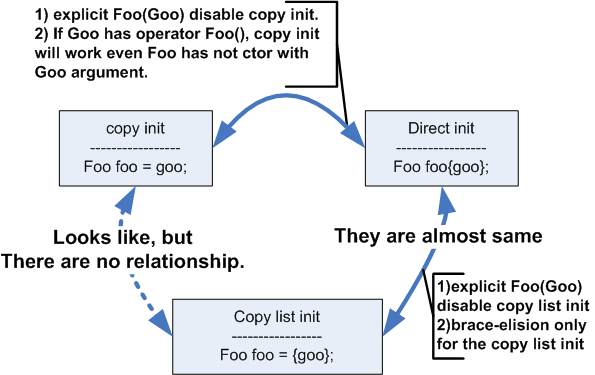
\includegraphics[width=0.45\linewidth]{pics/copy_list.png}
    \caption{difference between direct, copy and list-copy initialization.}
    \label{fig:copylist}
\end{figure}
	\item A good article is "Any difference between copy-list-initialization and traditional copy-initialization?"
\end{itemize}


\subsection{List initilization advantages}
			 
\begin{itemize}
	
	 \item Empty braces denote value initialization, which typically initializes types to binary zeros. Pay attention here, we can't use () instead of \{\}.
\begin{lstlisting}[numbers = none]
int i{};     //i becomes 0, can't use () here         
double d{}; //  d becomes 0.0, can't use () here        
int *p{};   //initialized to nullptr
char s[12]{}; // all 12 characters are initialized to '\0'
char *p=new char [5]{};  //all five chars are initialized to '\0'		
std::string s{}; // s becomes "" can't use () here  
std::vector<float> v{}; //v becomes an empty vector
\end{lstlisting}

    \item List initialization can avoid narrowing problem.
\begin{lstlisting}[numbers=none]
double val = 7.4;
int i {val}; //error, possible truncation.
\end{lstlisting}

    \item Creating anonymous variables in C++ is easy and can be useful for passing or returning values without the need for temporary variables. Anonymous objects are typically treated as rvalues, which means they do not have an address and can only be passed or returned by value or const reference. If you need to use the object more than once or take its address, you will need to create a named variable instead of an anonymous one.

\begin{lstlisting}[frame=single, language=c++]
Cents add(const Cents &c1, const Cents &c2){
	return Cents{c1.getCents() + c2.getCents()};
	// return anonymous Cents value
}

cout <<add(Cents{6}, Cents{8}).getCents();
\end{lstlisting}

    \item Using copy list initialization to pass or return values from a function without explicitly specifying the type can be future-proof. If you later rename the class, the copy list initialization using braces will continue to work as-is, while the copy list initialization using parentheses will require a name change.

\begin{lstlisting}
MyClass2 fun (MyClass2 m) 
fun(MyClass2(2011,3.14)) //before c++ 11, fun ( (2011,3.14) ) doesn't work

fun ( {2011,3.14} ){
	return {2011,3.14};  //there is ; in the end
}

MyClass2 mc2;
mc2 = {2011, 3.14}  // or MyClass2(2011, 3.14)
\end{lstlisting}

    \item List initialization supports a wide range of types with a uniform syntax, including aggregates, class members, and STL containers. Here are a few examples of how to use list initialization for these types:
\begin{lstlisting}[frame=single, language=c++,mathescape=true]
// C++98 
double *pd= new double [3]; // can't initialize them
rectangle w( origin(), extents() ); //vexing problem
vector<int>     v;  //need for loop to initialize it
for( int i = 1; i <= 4; ++i ) v.push_back(i);

// C++11 (note: "=" is mostly optional)
double *pd= new double [3] {0.5, 1.2, 12.99};
rectangle     w   = { origin(), extents() }; 
vector<int>   v   = { 1, 2, 3, 4 };
std::map<std::string,int> myMap{{"Scott",1976}, {"Dijkstra",1972}};	
\end{lstlisting}

    
    \item The uniform syntax provided by list initialization makes it easier to write generic template functions that can be used with a wide range of types. This isn't just an aesthetic issue; it can also have practical benefits when writing code that needs to be able to initialize any type. For example, when using perfect forwarding, the flexibility of list initialization can be especially useful:
 
\begin{lstlisting}[frame=single, language=c++,mathescape=true]
template<typename T, typename ...Args>
void forwarder( Args&&... args ) {
	T local = { std::forward<Args>(args)... };
	// ...
}
//All below statement can work because we have list initialization.
forwarder<int>            ( 42 );                  
forwarder<rectangle>      ( origin(), extents() ); 
forwarder<complex<double>>( 2.71828, 3.14159 );    
forwarder<mystruct>       ( 1, 2 );                
forwarder<int[]>          ( 1, 2, 3, 4 );          
forwarder<vector<int>>    ( 1, 2, 3, 4 );  	        
\end{lstlisting}


\item A non-static data member initializer (NSDMI) must use a brace-or-equal-initializer.
\begin{lstlisting}[frame=single, language=c++, mathescape=true]
class Foo{
public:
	Foo(): myData{1,2,3,4,5}{} // can initialize directly.
private:
	int myData[5];
	int equals = 42;                      //OK
	std::unique_ptr<Foo> braces{new Foo}; //OK
	std::vector<int> bad(6);  // 6 elements, all value are 0.
	std::vector<int> good{6}; // 1 element, value is 6. 
};
  	\end{lstlisting}
	

	\item A good reference article is GotW \#1 Solution: Variable Initialization or Is It? Another good one is Overview of C++ Variable Initialization. address is \\ \verb=https://greek0.net/cpp/initialization.html=
	
	\item \textbf{Summary of brace initialization advantage:}
\begin{enumerate}
	\item Provide value initialization automatically.
	\item Avoid narrowing problem.
	\item Avoid vexing problem. (Introduced in the next section.)
	\item Input and return temporary variable easier. Using \{\} directly without type name. 
	\item More uniform syntax, for aggregated, class member and STL container. 
\end{enumerate}
\end{itemize}


\subsubsection{Vexing parsing}
\begin{enumerate}
	\item The basic reason behind of vexing parsing come from C++ standard: \textbf{"If it can be a function declaration, it is".}
	
	\item Using parentheses to group variable names when declaring them is a legal and common practice in C++. This can be especially useful when declaring function pointers or other complex types. For example, to declare a function pointer, you must use parentheses to group the name of the function pointer and its arguments. Here are a few examples of how to use parentheses when declaring variables:
\begin{lstlisting}[frame=single, language=c++, mathescape=true]
int f(int);   //a function return a int
int *f(int);  //a function return pointer
int (*f)(int); //a function pointer;  
\end{lstlisting}
	
	\item It also means that you can have below C++ statements. Although unnecessary, but line 2 and line 4 are all legal statements.
\begin{lstlisting}[frame=single, language=c++, mathescape=true]
int x;
int (x); //same as above
int f(int x);
int f(int (x)); //same as above
\end{lstlisting}
	
	\item For function declaration, you can omit the parameter name.   
\begin{lstlisting}[frame=single, language=c++, mathescape=true]
int f(int x);
int f(int (x));
int f(int); //three statements are same. 
\end{lstlisting}
	
	\item For object, thing becomes interesting.
\begin{lstlisting}[frame=single, language=c++, mathescape=true]
int (x); // just like int x;

class A{
	A(int a);
...}
	
int a = 10; 
A(a); //you want to define a temporary object, but compile fail here. 
const A& ar = A(a); //this is OK

(A(a)); //If you really want a temporary A object, use another parentheses. 
\end{lstlisting}
\begin{description}
	\item[Line 8:] You want to create a temporary obj, but compile think it as A a; It trigger compiler error, redefine \texttt{a}, because \texttt{a} has been defined in line 7.
\end{description}
	
	\item From the perspective of the compiler, the following three function declarations are all interpreted as the same function:
\begin{lstlisting}[frame=single, language=c++, mathescape=true]
int f(double (*pf)()); //standard way
int f(double pf()); //You can omit parentheses, just like int x and int (x);
int f(double ()); //for function f, you can omit variable name.
\end{lstlisting}
\begin{description}
    \item[Line 2] Function arguments are adjusted to be a pointer to function arguments. That is only applicable in function parameter context. 
\end{description}

	\item After considering all the previous examples, it's understandable to feel confused when trying to use or define temporary C++ objects.
\begin{lstlisting}[frame=single, language=c++]
class Foo{
	......
};
	
Foo x(); //this is function declaration, you should use Foo x; or Foo x{};
	
Foo x(Foo());  // a function
Foo x(Foo (i)); //a function, Foo(i) equal Foo i; because () can be omitted by a compiler.
//vs.
Foo y{Foo{}};  // a variable, build with a temporary Foo
\end{lstlisting}
\begin{description}
	\item[Line 7:] declare a function \texttt{x}, receive a function pointer \texttt{Foo ()}, return \texttt{Foo}. Here, We omit the function parameter name, That is to say,  \texttt{Foo (*para) ()}  equals \texttt{Foo  ()} in this context.
	
	\item[Source code:]  Why \texttt{Foo(i)} equal \texttt{Foo i}; but \texttt{Foo()} equal a function pointer? If \texttt{Foo(int)}, then it will be a function pointer.  function declaration need type name, not a variable name, such as \texttt{i}.	
\end{description}

	\item Before C++11, you need add another pair parentheses to change it from declaration to expression. After C++11, you can use braces.
\begin{lstlisting}[frame=single, language=c++, mathescape=true]
Foo x{Foo{i}}; //x will not be translated into function declaration.   
Foo x{Foo{}}; //same as before. 
\end{lstlisting} 

	
	\item The most complex problem. A range container constructor. 
\begin{lstlisting}[frame=single, language=c++, mathescape=true]
list<int> data(istream_iterator<int>(dataFile), istream_iterator<int>()); //error
list<int> data(istream_iterator<int>{dataFile}, istream_iterator<int>{}));//OK
\end{lstlisting}
\begin{description}
	\item[Line 1:] \texttt{data} is function. First parameter is \texttt{dataFile}, type \texttt{istream\_iterator<int>}, second parameter is function pointer. The First, you can add () around parameter name;  the second, you can omit parameter name.
\end{description}
		
	\item The main reason for the vexing problem is that parentheses can be used to both grouping variable and function declarations, which can create ambiguity when declaring temporary objects. In other words, the vexing problem occurs when using parentheses and an unnamed temporary variable to initialize another variable. To fix this issue, we can use list initialization instead. A good reference is \verb|https://timesong-cpp.github.io/cppwp/n4140/stmt.ambig| or google search 
	"everything that can be a declaration is a declaration" 
	
\end{enumerate}



\section{Initializer\_list and auto}
\subsection{initializer\_list}
\begin{itemize}
	\item The problem originated from the way arrays are initialized in the C language, which cannot be used for C++ container objects. In generic programming, a "uniform initializer" is needed to enable consistent syntax for variables and arrays. To achieve this, C++11 introduced the \texttt{std::initializer\_list} template, which acts as a proxy class. We can define a constructor for a vector that takes an \texttt{initializer\_list} parameter to enable uniform initialization.
\begin{lstlisting}[frame=single, language=c++,mathescape=true]
int array[] = {1,2,3,4,5}  //OK 
vector<int> vt = {1,2,3,4,5} //doesn't work before C++11 

vector( std::initializer_list<T> init)
vector<int> vt = {1,2,3,4,5} //Work, call previous constructor
\end{lstlisting}
		
	\item In STL library container, \texttt{list}, \texttt{vector}, \texttt{map} support \texttt{initializer\_list} constructor. You also can use it in your own class, function or for range.
\begin{lstlisting}[frame=single, language=c++,mathescape=true]
void f(const initializer_list<string> &slst){
	....
}
f({ "Good", "morning", "!" });
	
// A braced-init-list can be implicitly converted to a return type.
vector<int> test_function() { return {1, 2, 3}; }
	
for (int i : {-1, -2, -3}) {} // Iterate over a braced-init-list.
	
void TestFunction2(vector<int> v) {}
TestFunction2({1, 2, 3}); // Call a function using a braced-init-list.
\end{lstlisting}

	\item  You should not only judge \texttt{initializer\_list} by braces. 1) \texttt{initializer\_list} should be class constructor parameter. 2) It uses braces to initialize. 3) The number of parameter inside braces is flexible but the type should be the same.

\begin{lstlisting}[frame=single, language=c++,mathescape=true]
vector( std::initializer_list<T> init)
vector<int> vt = {1,2,3,4,5} //call the constructor in line 1.
	
struct A{
	int i;
	int j;
};	
A a = {1, 2} // list initilization, don't use  initializer_list
\end{lstlisting}
	
	\item Mostly, list initilization and \texttt{initializer\_list} can be used together. For example if you want to initialize a map you can use an \texttt{initializer\_list} of list initialization of the key value pairs: Here, the type of the pairs is clear and the compiler will deduce, that '{"Alex", 522}' in fact means \texttt{std::pair<std::string const, int>\{"Alex", 522\}}.
	
\begin{lstlisting}[frame=single, language=c++,mathescape=true]
std::map<std::string, int> scores{ 
	{"Alex", 522}, {"Pumu", 423}, {"Kitten", 956} 
};
\end{lstlisting}

	\item An empty pair of braces can indicate either value initialization or an empty \texttt{std::initializer\_list}, so it's important to know how to distinguish between the two.
\begin{lstlisting}[frame=single, language=c++,mathescape=true]
class Widget{
	...
	Widget(){cout<<"default";}
	Widget(initializer_list<int>){cout<<"init";}
};
Widget w1; // calls default constructor.
Widget w2{};  //calls default constructor too.
	
Widget w4({});//std::initializer_list constructor with empty list 
Widget w5{{}}; //Same
\end{lstlisting}
	
	\item When non-empty list initialization is used and there are overload \texttt{initializer\_list}.
	\textbf{it always match initializer\_list}.
\begin{lstlisting}[frame=single, language=c++,mathescape=true]
class Widget {
public:
	Widget(int i, bool b); // as before
	Widget(int i, double d); // as before
	Widget(std::initializer_list<long double> il);
};
	
Widget w1(10, true); //  calls first constructor
Widget w1{10, true}; // std::initializer_list constructor
// (10 and true convert to long double)

Widget w2(10, 5.0); //  calls second constructor
Widget w2{10, 5.0}; // std::initializer_list constructor
// (10 and 5.0 convert to long double)
\end{lstlisting}
\begin{description}
    \item[Line8-9] Compilers' determination to match braced initializers with constructors taking \\ \texttt{std::initializer\_lists} is so strong, it prevails even if the best-match \\ \texttt{std::initializer\_list} constructor can't be called.
\end{description}
	
	\item An example that highlights semantic difference between parentheses and braces is the vector class. When initializing a vector with a list of values to be stored in the object (such as the elements of a vector), it is recommended to use curly brace initialization. On the other hand, if the values are used to describe the intended value/state of the object (such as the size argument of a vector or the file name argument of an fstream), it is recommended to use parentheses. In other words, if the constructor behaves like a normal function call with some additional, parameterized operations, then it's preferred to use parentheses. For instance, the size argument of a vector or the file name argument of an fstream fall under this category..
	
\begin{lstlisting}[frame=single, language=c++,mathescape=true]
std::vector<int> v1(10, 20);  //create 10-element vector, all elements 20.
std::vector<int> v2{10, 20};  //create 2-element vector, element are 10 and 20
\end{lstlisting}
		
	
\end{itemize}

\subsection{Auto initilization(Almost Always Auto)}

\subsubsection{Basic usage}
\begin{itemize}
	\item Three main usage of \texttt{auto}:
	\begin{enumerate}
		\item Initialization. For example, you can assign lambda to an auto type.
		\item \texttt{auto} parameter in lambda.
		\item \texttt{auto} return type.  with help of \texttt{auto} parameter and \texttt{auto} type, you can build \textbf{generic lambda}. in this field, you need to know when to use \texttt{decltype(auto)}.
	\end{enumerate}

	\item Auto initialization sets the type of a declared variable from its initializing expression at compile-time. It is recommended to use 'auto' when initializing a variable with an expression.
\begin{lstlisting}[numbers=none]
auto a = expr
auto a = T{expr} //when you want to commit to type

auto s = "Hello";  //s is const char* just like const char* s = "Hello";
auto str = string{"Hello"} // this time is string
auto p = &x  //prefer to use auto* p, because it stresses the intent
auto v = {1, 2, 3}    // std::initializer_list
auto vect = vector<int>{1,2,3} // this time is vector.

auto p = new vector<pair<int, string> >; //don't need pointer type
std::vector<std::pair<int, std::string>> array;
auto it = array.begin();    //don't need container iterator type
//unique_ptr<widget> w = make_unique<widget>();
auto w = make_unique<widget>(); //template class or function.

auto l = [](){..}; //lambda
double fm(double, int);
auto pf = fm  //pf is function pointer.        
\end{lstlisting}
	
	\item About the auto \texttt{type} deduction, please refer to the next chapter Generic programming type inference section. The basic idea is quite simple: take exactly the type on the right-hand side, but strip off top-level const/volatile and reference \&/\&\&. If you want your auto declaration to be \texttt{const}, or if you want your \texttt{auto} declaration to be a reference, you have to add them explicitly.
	
\begin{lstlisting}[frame=single, language=c++]
const auto iter = modmap.find(123); //specify const
auto& mod = vec[17];      //specify &
for (const auto& element : myarray) {
	//do stuff that reads from element
}
\end{lstlisting}
	
	\item \texttt{auto} can be used in template function return type.
\begin{lstlisting}
template <typename F, typename T>
auto apply(F&& f, T value){
	return f(value);
}
\end{lstlisting}

	\item Four advantages of using \texttt{auto}:
	\begin{enumerate}
		\item Avoidance of uninitialized variables.
\begin{lstlisting}[numbers=none]
auto x2; // error! initializer required
auto x3 = 0; // fine, x's value is well-defined
\end{lstlisting}

		\item Avoidance of verbose variable declarations.
\begin{lstlisting}[frame=single, language=c++]
template<typename It>
void dwim(It b, It e) {
//typename std::iterator_traits<It>::value_type currValue = *b;
auto currValue = *b; //using auto is simple
	
auto ii = find_if(people.begin(), people.end(), match_name );               
if (ii != people.end()){...}
\end{lstlisting}

		\item Avoid what I call problems related to "type shortcuts." It's very importance here, it guarantee correct and performance.
\begin{lstlisting}[frame=single, language=c++]
std::vector<int> v;
		...
int sz = v.size(); 
auto sz = v.size(); //v.size() return size_t, not int
		
std::unordered_map<std::string, int> m;
for (const std::pair<std::string, int>& p : m){
	... 
}  //pair type should be pair<const std::string, int>

for (const auto& p : m){
	... // as before
} //fix the previous error.
\end{lstlisting}

	\item Good maintenance. First, change id type in line 3 to line 4, if we use \texttt{auto} in line 8, we don't need to change at all. But if we use \texttt{int}, then we need to change from \texttt{int} to \texttt{GUID} too.
\begin{lstlisting}[frame=single, language=c++, mathescape=true]
struct record {
	std::string name;
	int id;
	//GUID id; 
};

//int id =  find_id(const std::vector<record> &people...
auto id = find_id(const std::vector<record> &people, const std::string &name)
\end{lstlisting}
	\end{enumerate}
\end{itemize}
	
\subsubsection{pitfall of auto}
	There are two points need to be noticed. The first one is using \texttt{auto} with \texttt{vector<bool>}, The second is combining \texttt{auto} with list initialization.
	\begin{enumerate}
		\item "invisible" proxy classes. An invisible proxy class example is \texttt{vector<bool> operator []}. \\ \texttt{vector<bool>::operator[]} neither yields a bool nor a reference to a bool. It just returns a little proxy object that acts like a reference. This is because there are no references to single bits and vector<bool> actually stores the bools in a compressed way. So by using auto you just created a copy of that reference-like object. The problem is that C++ does not know that this object acts as a reference. You have to force the "decay to a value" here by replacing auto with T.  If you don't understand why, no worry. I will introduce \texttt{std::ref} in the Concurrent chapter, you can go there to look the introduction of \texttt{std::ref}. Both "proxy" class and \texttt{std::ref} share the same idea.
\begin{lstlisting}
template <typename T>
void Test(const T& oldValue, const T& newValue, const char* message){
	vector<T> v;
	v.push_back(oldValue);
	auto x = v[0]; // for vector<bool> get proxy class
	x = newValue;
}
Test<int>(10, 20, "Testing vector<int>"); // no change v[0]
Test<bool>(true, false, "Testing vector<bool>"); //change v[0]
\end{lstlisting}
\begin{center}
	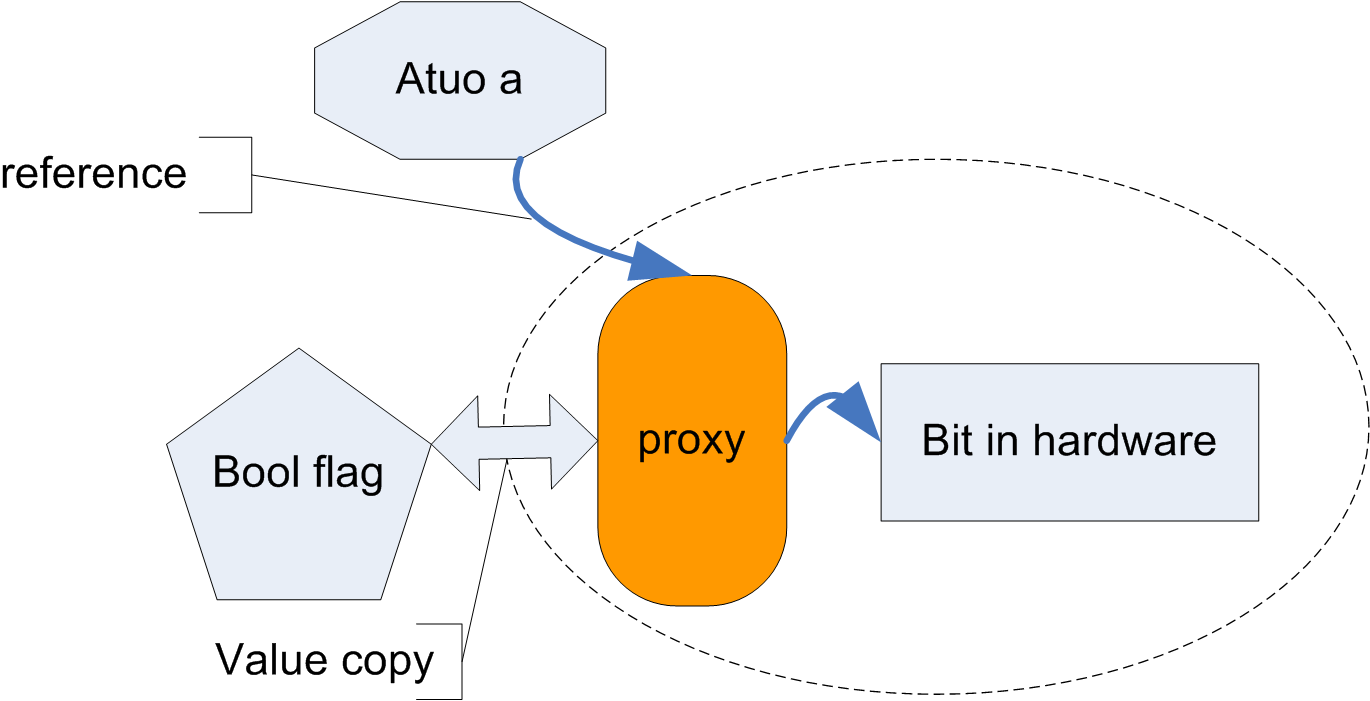
\includegraphics[width=0.45\linewidth]{pics/auto2.png}
\end{center}

		\item Initialization brace return \texttt{std::initializer\_list<int>}. Prior to C++17 the type for all the following objects (a, b, c and d) is deduced to \texttt{std::initializer\_list<int>}. There is no difference between the direct-list-initialization and the copy-list-initialization on the result of the type deduction.  After C++ 17, For copy list initialization auto deduction will deduce a \texttt{std::initializer\_list<T>} if all elements in the list have the same type, or be ill-formed. For direct list initialization auto deduction will deduce a T if the list has a single element, or be ill-formed if there is more than one element.  In another word, When you use = and \{\} together, it will deducted as \texttt{std::initializer\_list}, no matter how many parameters are there inside the \{\}. If you want to avoid \texttt{std::initializer\_list}, \textbf{please don't use =}. 
		
\begin{lstlisting}[numbers=none]
auto a = {42};   // std::initializer_list<int> //Before C++ 17
auto b {42};     // std::initializer_list<int> //not nature
auto c = {1, 2}; // std::initializer_list<int>
auto d {1, 2};   // std::initializer_list<int>

auto a = {42};   // std::initializer_list<int>// After C++ 17
auto b {42};     // int
auto c = {1, 2}; // std::initializer_list<int>
auto d {1, 2};   // error, too many 
auto e = { 1, 2.0 }; // error: cannot deduce element type
\end{lstlisting}

\end{enumerate}


\section{Initialization Examples}

\subsection{How to analyze initialization expression}
\begin{itemize}
	
	\item List initialization must be able to handle different kinds of types, such as built-in types, aggregates, and classes with different constructors. This adds complexity to the analysis, and it's important to read the C++ reference carefully to analyze the initialization syntax step by step.
\begin{lstlisting}
A a{}; //value initilization
A a{1};	 // direct initilization or aggregate initilization depends on A type	
\end{lstlisting}		
	
	
	\item I will provide a real example to demonstrate how to analyze a complex initialization statement with help of a reference to the C++ standard document for further understanding.
\begin{lstlisting}
struct A {
	A(int i) : i(i) {}
	A() = default;
	int i;
};

A a{};  //a.i is 0, not random value	
\end{lstlisting}	
	
	\begin{description}
		\item[Line 7:]  The list initialization of \texttt{A}, Why it's list initilization? Because it use \{\}; *1 item satisfied, so perform value initialization. Please note here, *1~*5 item refer to "Excerpts from C++ standard" below. Check *3 item, not satisfied, because we have default constructor. Then it meets all requirements in *4 item, so perform zero-init.
	\end{description}
	
\begin{lstlisting}
struct A {
	int i;
	int j;
};
cout<<is_aggregate_v<A><<endl; //output: 1
A a{1};  //  i = 1, j = 0;	
\end{lstlisting}	
	
	
	\begin{description}
		\item[Line 7] List initialization of A, Check *1 item but fail, \texttt{A} has no default constructor. \texttt{A} is aggregated type, according to *2 item, aggregate-initialization kick off. According to *5 item, \texttt{j} is initialized to 0		
	\end{description}
	
	\item  Excerpts from C++ standard: 
				
	{\footnotesize \verb|https://en.cppreference.com/w/cpp/language/list_initialization| \newline
	*1 (\textbf{For list initialization})If the braced-init-list is empty and T is a class type with a default constructor, value-initialization is performed. 
	\newline
	*2 Otherwise, if T is an aggregate type, aggregate initialization is performed.
	
	
	\verb|https://en.cppreference.com/w/cpp/language/value_initialization|	\newline
	*3 if T is a class type with no default constructor or with a user-provided or deleted default constructor, the object is default-initialized; 
	\newline		
	*4 if T is a class type with a default constructor that is neither user-provided nor deleted (that is, it may be a class with an implicitly-defined or defaulted default constructor), the object is zero-initialized and then it is default-initialized if it has a non-trivial default constructor; 
	
	\verb|https://en.cppreference.com/w/cpp/language/aggregate_initialization|\newline
	*5 If the number of initializer clauses is less than the number of members and bases (since C++17) or initializer list is completely empty, the remaining members and bases (since C++17) are initialized by their default member initializers,}


	
	\item Based on previous three levels theory, you can follow below logic to analyze C++ initialization.
	\begin{center}
		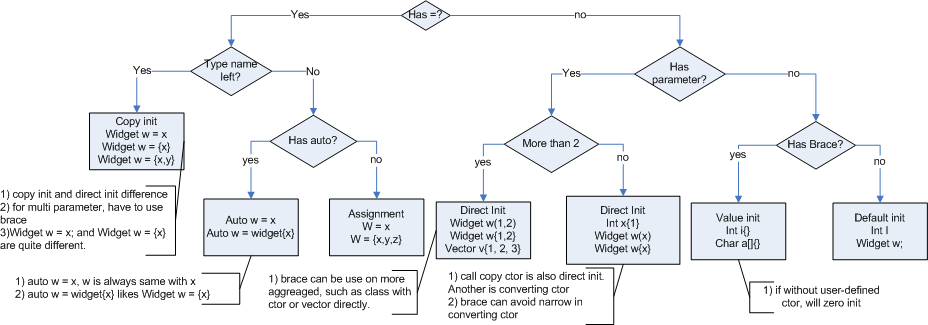
\includegraphics[width=0.95\linewidth]{pics/init.png}
	\end{center}
		
\end{itemize}

\subsection{Common used forms in initialization}

\begin{itemize}
	
	\item Detail syntax analysis and comparison.
\begin{lstlisting}[frame=single, language=c++,mathescape=true]
widget w;               // (a)
widget w();             // (b)
widget w{};             // (c)

widget w(x);            // (d)
widget w{x};            // (e)

widget w = x;           // (f)
widget w = {x};         // (g)

auto w = x;             // (h)
auto w = widget{x};     // (i)
\end{lstlisting}	
	
	\begin{enumerate}
		\item (a) is just default initialization with default constructor.
		
		\item \textbf{(b) is function declaration.} That is why we prefer use brace initialization (c), it will avoid this vexing problem.
		
		\item For (d) and (e), These are both direct initialization. The variable w is initialized "directly" from the value of x by calling \texttt{widget::widget(x)}. If x is also of type widget, this invokes the copy constructor. Otherwise, it invokes a converting constructor.
		
		\item (e) is better than (d) to avoid narrowing, for example: \texttt{int a(1.2)} pass, but \texttt{int a{1.2}} fail.
		
		\item For (e), it prefer constructor that takes an \texttt{initializer\_list.} We will introduce more in \texttt{initializer\_list.} section.
		
		\item For (f), when \texttt{x} is type of widget, just like (d), but can't work when copy constructor is explicit(copy constructor never be explicit). When \texttt{x} is not type of widget, it will convert \texttt{x} to a temporary If \texttt{x} is of some other type, \textbf{conceptually} the compiler first implicitly converts x to a temporary widget object, then move-constructs w from that temporary rvalue, using copy construction as "the slow way to move" as a backup if no better move constructor is available. Assuming that an implicit conversion is available, (f) means the same as widget w( widget(x) );. Note that I said "conceptually" a few times above. That's because practically compilers are allowed to, and routinely do, optimize away the temporary and, if an implicit conversion is available, convert (f) to (d), thus optimizing away the extra move operation. However, even when the compiler does this, the widget copy constructor must still be accessible, even if is not called, the copy constructor's side effects may or may not happen.
		
		\item \textbf{For (g), This is called “copy list initialization.” It means the same as \texttt{widget w\{x\}};} except that explicit constructors cannot be used. It’s guaranteed that only a single constructor is called,(only converting constructor is called, no copy constructor).
		
		\item (h) just like type-of-x w(x), is same with (d), only single copy constructor is called
		
		\item (i) is the most consistent spelling when you do want to commit to a specific type and explicitly request a conversion if needed, and once again the \{ \} syntax happily avoids lossy narrowing conversions. In practice on most compilers, only a single constructor is called-similarly to what we saw with (f) and (g).
		
		\item Some initialization examples based on previous introductions.
		
\begin{lstlisting}[frame=single, language=c++,mathescape=true]
class Test{
public:
	int i;
	explicit Test(int a = 0):i(a){}
	Test(const Test &T){ cout<<"copy constructor";} 
};

Test too = 2;  //test for (f) 
Test too = {2} // test for (g)

Test too;  
auto w = too //test for (h)
auto w = Test{2} //test for (i), no semantic difference with Test w{2};	
\end{lstlisting}		
		\begin{description}
			\item[Line 8 and 9:] Both (f) and (g) work and no call copy constructor (no output:"copy ctor"); If converting ctor has explicit both fail,but \texttt{Test too\{2\}} succeed; if copy constructor is private, (f) fail, but (g) is still OK. Because \texttt{A a = \{b\};} is just like \texttt{A a(b);}
			
			
			\item[Line 13:] you can use \texttt{auto w = Test(2)}, it just call converting constructor, even converting constructor is explicit, it can work too. No copy constructor is called at all. \texttt{w} is not const reference. List initilization \{\} is better, it more generic and avoid narrow \texttt{auto w = Test\{1.2\}} fail, 
		\end{description}
		
	\end{enumerate}

	\item Given below code snippet, the syntax analysis for the default constructor is given below.
	
\begin{lstlisting}[frame=single, language=c++]
class A{
public:
	A(){};
	A(int k):m_a(k){};
	A(const A& rhs){m_a = rhs.m_a;};
	int m_a;
};
void fun(const A &a){}
int i = 3;	
\end{lstlisting}		
	

	\begin{tabular}{|p{0.23\textwidth}|p{0.68\textwidth}|}
		\tophline
		Expression & Syntax analysis \\
		\tophline
		\texttt{A a, A a\{\}} & \texttt{a} is object, call default constructor. \\
		\tophline
		\texttt{A a()} & \textbf{declare function a,vexing problem happens here.} \\
		\tophline
		\texttt{A()} & A temporary A obj or declaration, detail is in vexing problem \\
		\tophline
		\texttt{B b(A())} & \textbf{declare function, vexing problem}, A() is function pointer \\
		\tophline
		\texttt{B b(A\{\})} & construct \texttt{b} object with temporary A object. \\
		\tophline
		\texttt{fun(A()),fun(A\{\})} & pass a temporary \texttt{A} object to \texttt{fun} 
		\bottomhline
	\end{tabular}
	
	\item The syntax analysis for the single parameter constructor is given below. 
	
	\begin{tabular}{|p{0.23\textwidth}|p{0.68\textwidth}|}
		\tophline
		Expression & Syntax analysis \\
		\tophline
		\texttt{A a(i), A a\{i\}} & parameterized constructor, direct initialization\\
		\tophline
		\texttt{A (i)} & \textbf{just like \texttt{A i}, you have define \texttt{i}, so compiler barks.} \\
		\tophline
		\texttt{A\{i\}} & A temporary A obj\\
		\tophline
		\texttt{B b(A(i))} & declare a function \texttt{B b(A i)}; vexing problem \\
		\tophline
		\texttt{B b(A\{i\})} & build \texttt{b} with temporary \texttt{A} object \\
		\tophline
		\texttt{fun(A(i)),fun(A\{i\})} & work, fun(A i) will not a declaration, because there are no return value.\\
		\tophline
		\texttt{B b(A a(i))}  & compile error, because \texttt{A a(i)} is not a expression(it doesn't yield a value). Compiler will first interpret it as function declaration first, but \texttt{A a(i)} is not declaration (it defines a variable a), ( \texttt{A(i)} and \texttt{A()} are both type). So it continue to interpret as B constructor, then it ask a value from expression, but \texttt{A a(i)} is not expression either, in the end, compiler is not happy.  \\
		\tophline
		\texttt{fun(A a(i))} & Same as above.
		\bottomhline
	\end{tabular}
	
	%	\item Further explanation about previous table. Here we follow the basic C++ parsing rule: \textbf{If there is possible, it will use declaration first. }.
	%\begin{lstlisting}
	%int i = 5;
	%A(i); //redefine variable i, just like A i; compiler error
	%A a = A(i);
	%B b(A(i)); //function delcaration
	%B b(A a(i)); //compile fail
	%\end{lstlisting}	
	%	\begin{description}
	%		\item[Line 3:] \texttt{A(i)} will build temporary \texttt{A}, because there is assignment sign, so \texttt{A(i)} can't be declaration, otherwise it can't be suitable for the context.
	%		
	%		\item[Line 4:] interpret \texttt{A(i)} as declaration, and it suitable for the context.
	%		
	%		\item[Line 5:] For \texttt{B b(A a(i))}, 
	%	\end{description}
	
		 \item A good article about this is "Initialization in C++ is Seriously Bonkers"
\end{itemize}

\section{Initialization summary}

\subsection{Key points of this chapter}
\begin{itemize}
	\item Understanding some basic conceptions. such as aggregate type. copy-list-initilization, converting constructor. All the high level usages are based on these basic conceptions. 
	
	\item Familiarity with the basic six initialization methods is important. You should know how to distinguish them, for example, when using the equal sign, it is called copy initialization.
	
	\item Six initilization methods and list initialization are irrelevant. List initialization syntax can be interpreted as aggregated init, value init, direct initialization or copy initialization and it brings its own advantage.
	
	\item Know the difference between value initialization and default initialization. Know the difference between direct init, copy initialization and list copy initialization.  
\begin{lstlisting}
A a(1) or A a{1} //direct init
A a = 1;  //copy init
A a = {1}; //list copy init, same as direct init	
\end{lstlisting}	
		 
	\item Know when to use list initialization and it's advantage. Know the basic usage of \texttt{initializer\_list} and the difference between list initialization. just pay attention when the class has \texttt{list\_initiaizer} constructor know the auto usage and its pitfall.
	
	\item There are three levels of initialization knowledge in C++. The first level is the syntax level, which determines whether we use braces or parentheses, an assignment operator, or a function return, among other things. From this level, we can go deeper to another level to determine what kind of initialization methods are available. There are six different methods. Finally, we can reach the semantic level, which depends on the specific data type for the detailed initialization action.
	
	For example, if T is an aggregate type, we use aggregate initialization. If the braced-init-list is empty and T is a class type with a default constructor, we use value-initialization. In other words, '\texttt{A a\{x, y\}}' may be a direct initialization or an aggregate initialization, depending on the data type and syntax. This is an essential point for you to understand better about initialization in C++.
	
	
\begin{center}
	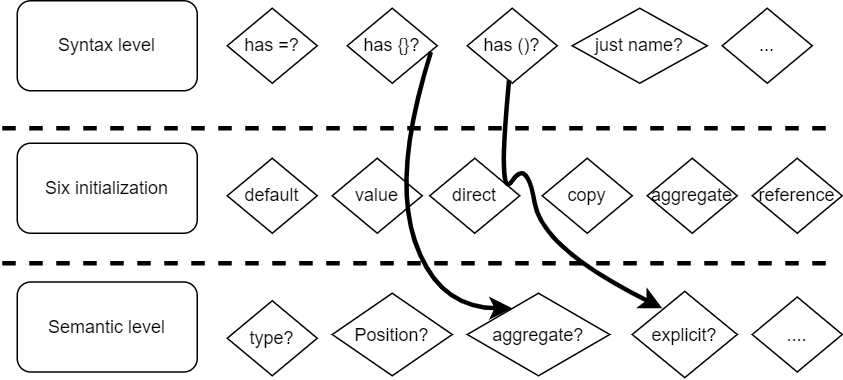
\includegraphics[width=0.60\linewidth]{pics/sum_init.png}
\end{center}	
			
\end{itemize}


\subsection{Initialize suggestions}

\begin{itemize}
		\item Even if you don't understand the whole chapter on initialization, you can still follow these steps when you need to initialize a variable in C++:
		
	\begin{enumerate}
		\item If right side is expression, new or function, Use \textbf{\texttt{auto var = expr;}}. 
		
		\item Otherwise, Use \textbf{list initialization if possible.}   Default initialization, use \{\}. Maybe it's redundant for some types, but it's good habit and keep your style consistency. For example, use \texttt{String str\{\}} instead of \texttt{String str}. 
		
		\item When using list initialization, pay attention two traps for \texttt{std::initilizaer\_list.} 
		\begin{enumerate}
			\item If type has list initialization constructor, list initialization will use it first, and very strongly. 
			
			\item When we combine \texttt{auto} and list initialization together, it maybe deducts \\ \texttt{std::initilizaer\_list} type, maybe not.  You can see the section "pitfall of auto" 
		\end{enumerate}
		
		\item If the (single) value you are initializing with is intended to be the exact value of the object, use copy (=) initialization (because then in case of error, you'll never accidentally invoke an explicit constructor, which generally interprets the provided value differently).
\begin{lstlisting}
Foo f1 = f2; //best style
Foo f1(f2);  
Foo f1 = {f2};  
\end{lstlisting}		
		\begin{description}
			\item[Line 2:] If f2 is not Foo type, then line 1 will fail with explicit single parameter constructor, but Line 2 will implicit convert and pass. That is not good.
			
			\item[Line 3:] It is just like line 2, it will fail with explicit single parameter constructor, but semantic is not as good as line 1.
		\end{description}
		
	\end{enumerate}

\item The whole idea can be illustrated by below graph:
\begin{center}
	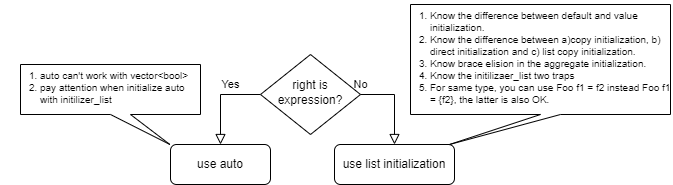
\includegraphics[width=1.0\linewidth]{pics/init_trip.drawio.png}
\end{center}


	
	
%		\item Basic rules:
%	\begin{enumerate}
%		\item If the (single) value you are initializing with is intended to be the exact value of the object, use copy (=) initialization (because then in case of error, you'll never accidentally invoke an explicit constructor, which generally interprets the provided value differently). In places where copy initialization is not available, see if brace initialization has the correct semantics, and if so, use that; otherwise use parenthesis initialization (if that is also not available, you're out of luck anyway).
%		
%		\item If the values you are initializing with are a list of values to be stored in the object (like the elements of a vector/array, or real/imaginary part of a complex number), use curly braces initialization if available. 
%		
%		\item If the values you are initializing with are not values to be stored, but describe the intended value/state of the object, use parentheses. In another word, if the constructor resembles a normal function call (it performs some more or less complex operations that are parameterized by the arguments) then using the normal function call syntax(parentheses). Examples are the size argument of a vector or the file name argument of an fstream. 
%		
%\begin{lstlisting}
%vector<int> b{10,20}; //fills the vector with the arguments
%vector<int> c(10,20); //uses arguments to parameterize some functionality, Like filling the vector with 10 integers.
%vector<int> d{}; 
%\end{lstlisting}
%		\begin{description}
%			\item[Line 3:] Default initialization, use \{\}. For vector, maybe it's redundant, but it's good habit and keep your style consistency. For example, \texttt{int i}; and \texttt{int i\{\}}.
%		\end{description}
%	\end{enumerate}
%
	
\end{itemize}


\chapter{Memory}

\section{Memory functions in C}

\begin{itemize}
	\item That is a long story. In the C language, what happens if you forget a header file? In short, it will produce a warning in C99, but not in C89, and the compiler will assume the "implicit int" rule. This means that it presumes a function without a prototype (declared in the header file) will simply return an \texttt{int} type. Based on these rules, if you comment out \texttt{stdlib.h} in the code below, the compiler will assume that \texttt{malloc} returns an \texttt{int}. This code will run on a 32-bit computer because \texttt{int} and \texttt{int*} have the same length. However, on a 64-bit computer, \texttt{int*} is 64-bit and \texttt{int} is 32-bit, so half the data will be lost and your code will crash. What's worse is that if you add an \texttt{(int*)} cast, it will suppress the warning message. By doing so, you are effectively killing the only clue that something is wrong, which is not a good practice.
\begin{lstlisting}[frame=single, language=c++]
// include "stdlib.h"
int *sieve = (int *)malloc(sizeof(int)*length);	
int *sieve = malloc(sizeof(int)*length);
\end{lstlisting}
\begin{description}
	\item[Line 2:] With explicit cast, it will NOT produce a (missing prototype)warning.
	\item[Line 3:] Without explicit cast, it will produce a warning.
\end{description}

	\item We don't recommend using the \texttt{(int*)} cast at all. The next question is whether malloc actually returns \texttt{void*} and whether \texttt{void*} can be implicitly cast to \texttt{int*} or other pointer types in assignment. The answer is \textbf{YES}.
	
	\item In C language, we can use \texttt{NULL} to initialize pointer type.
\begin{lstlisting}[numbers=none]
#define NULL ( (void*) 0)
int *p = NULL;  //legal
FILE * f = NULL;  //legal
\end{lstlisting}
	
	\item In C++, the statement \texttt{int *p = (void *) 0} is not legal anymore since C++ is a type-safe language. Therefore, in C++, the literal \texttt{NULL} is defined as 0. However, this creates another ambiguity problem. To resolve this problem, C++11 introduced the keyword \texttt{nullptr}.
\begin{lstlisting}[numbers=none]
int *p = NULL; //illegal in C++

cout<<is_integral<decltype(nullptr)>::value; //false
cout<<is_integral<decltype(NULL)>::value; //true
\end{lstlisting}

	
\begin{lstlisting}[numbers=none]
int *p = NULL; //illegal in C++
--------------------------------------
f(int i)
f(int * p);

f(NULL);  //will call f(int i).
f(nullptr) //will call f(int *p)
\end{lstlisting}
	
	\item \texttt{calloc()} zero-initializes the buffer, while \texttt{malloc()} leaves the memory uninitialized. Zeroing out the memory may take a little more time, so you probably want to use \texttt{malloc()} if that performance is an issue. If initializing the memory is more important, use \texttt{calloc()}. For example, \texttt{calloc()} might save you a call to \texttt{memset()}.
	
	\item When you use \texttt{memcpy}, the destination cannot overlap the source at all, but \texttt{memmove} can. This means that \texttt{memmove} might be very slightly slower than \texttt{memcpy}, as it cannot make the same assumptions. For example, \texttt{memcpy} might always copy addresses from low to high. If the destination overlaps after the source, this means some addresses will be overwritten before copied. \texttt{memmove} would detect this and copy in the other direction - from high to low - in this case. However, checking this and switching to another (possibly less efficient) algorithm takes time.
	
	\item Reallocates the given area of memory. It must be previously allocated by \texttt{malloc()}, \texttt{calloc()} or \texttt{realloc()} and not yet freed with a call to free or \texttt{realloc}. Otherwise, the results are undefined. realloc may or may not change the original address. 

\begin{lstlisting}[]
str = (char *) malloc(15);
strcpy(str, "tutorialspoint");
printf("String = %s,  Address = %p\n", str, str);

/* Reallocating memory */
str = (char *) realloc(str, 25);
strcat(str, ".");
printf("String = %s,  Address = %p\n", str, str);
\end{lstlisting}
	
	\item Don't return the value assigned to the input pointer \texttt{ptr}. Instead, use another local pointer, such as \texttt{new\_ptr}, because if \texttt{realloc} fails, it will not overwrite the original \texttt{ptr}."
\begin{lstlisting}[numbers=none]
void *new_ptr = realloc(ptr, new_size);
if (!new_ptr) {
	// deal with error;
}
ptr = new_ptr
\end{lstlisting}
\end{itemize}


\section{new operator in C++}
\subsection{Basic}
\begin{itemize}
	\item There are four sub-topics related to the new operator: 1) new\_handler, 2) no throw, but return \texttt{nullptr} (since C++11), 3) placement new (which does not allocate, only constructs), and 4) operator new (which only allocates, without constructing). For the default new operator, you can use \texttt{set\_new\_handler} to adjust the behavior when enough memory cannot be allocated. More details can be found in the next section.
\begin{lstlisting}[frame=single, language=c++]
std::set_new_handler(noMem);
MyClass* p1 = new MyClass;//call noMem if fail, throw exception if no new handler

MyClass * p2 = new (std::nothrow) MyClass; // no throw
new (p2) MyClass;   //placement new

MyClass * p3 = (MyClass*)::operator new (sizeof(MyClass));	
\end{lstlisting}
\begin{description}
	\item[Line 7:] operator new, allocates memory by calling: \texttt{operator new}. but does not call MyClass's constructor
\end{description}	

	\item The nothrow new operator only ensures that the operator new inside it will not throw an exception, but will return nullptr if the allocation fails. However, it does not guarantee that the constructor of MyClass will not throw an exception. Therefore, it is not a fully mature design. In other words, we do not recommend using this type of nothrow new operator in production code.

	\item The new operator will call the constructor function of a class, but \texttt{malloc} will not call the constructor function. Therefore, in C++, you should use the new operator instead of \texttt{malloc}.
		
	\item If you use \texttt{new int[100]}, don't forget to use \texttt{delete []} to deallocate the memory. Any time you want to use new to allocate an array, ask yourself if you can replace it with vector or string. If the answer is 'yes', don't use array new. When you have to use array new to allocate an array, you must use the array delete. If you don't use array delete, you may end up deleting only the first object in the array. If you use array delete on a single new, it's undefined behavior. The system will remember the size corresponding to \texttt{pa}. With [], it will iterate with the size. When you forget [], it will only free the first object, causing a memory leak."
	
\begin{lstlisting}[frame=single, language=c++]
Foo pa* = new Foo[10];
delete [] pa;
\end{lstlisting}	
	
	\item Basic logic of array new. An basic implementation can be found in "Inside the C++ Object Model" 6.2 chapter
\begin{lstlisting}[numbers=none]
vec_new(int elem_count, int size, funptr constructor){
	total_size = size*elem_count;
	ptr_array = new char[total_size];
	registrate pair of ptr_array elem_count to system
	while(elem<end of address){
		(*constructor)(elem) //call the ctor
		elem+=size;
	}
}	
\end{lstlisting}
	
	\item When you use array new with inheritance, there is one important thing to notice: don't use a base pointer to point to an array with a derived class. Why is it dangerous? When you use \texttt{delete [] bp}, the system will think that it's a base array, and each element in it is just a base object. Therefore, virtual functions won't play a role here. For more details, please refer to the 'Inheritance' section in this book. Note that \texttt{bp[2]} is not a pointer; polymorphism only works when we use a pointer or reference.
\begin{lstlisting}[frame=single, language=c++]
base *bp = new derived[10]; //always use derived *dp = new derived[10]
bp[2]  //dangerous, undefined. size is wrong: \texttt{bp+sizeof(base)*2}
delete [] bp; //dangerous, 1)size is wrong, 2)it will call base::~base()	

Base b, Derived d; //The whole idea is just like assigning Devirved to Base
b = d;  // slice happens, but  new and pointer hide the detail behind the scene.
\end{lstlisting}	
	
\end{itemize}

\subsection{new operator logic}
\begin{itemize}
    \item When you call the new operator, it calls operator new, and operator new calls new\_handler. This gives you two opportunities to customize the behavior of the operator: you can customize operator new and you can customize new\_handler.
    
	\item Basic logic of new operator and delete operator. Below are C++ pseudo code.
\begin{lstlisting}[]
Point3d *origin = new Point3d;
	
if(origin = operator new(sizeof(Point3d))){ //operator new to allocate memory
	try{
		origin = Point3d::Point3d(origin); //call constructor
	}
	catch(...){  //if constructor throw an exception, no memory leak
		operator delete(origin);
		throw
	}
}
\end{lstlisting}
	
\begin{lstlisting}[]
delete origin;
	
if (origin != NULL) {
	origin->~Foo(); //destructor can't be private or protected
	operator delete(origin);
}
\end{lstlisting}
	
\item Basic logic of operator new. This is throw version operator new, non-throw and placement operator new are quite alike. 
\begin{lstlisting}[frame=single, language=c++]
void * operator new(std::size_t size) throw(std::bad_alloc){
using namespace std; 
	if (size == 0){ //handle 0-byte requests by treating them as 1-byte request   
		size = 1;             
	}                 
	void *last_alloc;
	while (true) { //continue to try allocate memory.
		*last_alloc = malloc(size)
		if (last_alloc)
			return last_alloc;
		new_handler globalHandler = set_new_handler(0); 
		set_new_handler(globalHandler); // allocation was unsuccessful,
		if (globalHandler)           //find current new-handling function
			(*globalHandler)();      // and call it.
		else 
			throw std::bad_alloc();
		}
}
	\end{lstlisting}
\begin{description}	
    \item[Source code:] Why we need to call \texttt{set\_new\_handler} twice, The first one get the current handler, and the second one changes it back. That is only way we can get the current handler. This idiom is also used in \texttt{set\_terminate} and \texttt{set\_unexpect}. Most of time, we use \texttt{malloc} and \texttt{free} to allocate and free physical memory. In C++11, introduce \texttt{get\_new\_handler()} function. We don't need to call \texttt{set\_new\_handler} twice. 
\end{description}

\item Basic logic of operator delete.
\begin{lstlisting}[numbers=none]
operator delete (void *ptr){
	if (ptr)
		free(ptr)
	}
\end{lstlisting}
	
	\item An example of a function pointer in the C++ standard library is \texttt{set\_new\_handler}. It accepts a function pointer and returns the same function pointer, which can make declaring this type of function a little difficult.
\begin{lstlisting}[frame=single, language=c++]
void failNew(){
	cerr<<"operator new fail!!!"<<endl
	abort();
}
-----------------------------------------
extern void ( *set_new_handler ( void (*)() ) ) (); //complex declaration.	
set_new_handler(failNew);

typedef void(* FunPtr)();  //A better method is to use typedef
FunPtr (*set_new_handler) (FunPtr);
set_new_handler(failNew);
\end{lstlisting}
		
	

	\item At program startup, the value of \texttt{new\_handler} is a null pointer. If an allocation fails inside of operator new, and\texttt{ std::get\_new\_handler} returns a null pointer value, then operator new will throw \texttt{std::bad\_alloc}.
	
	\item As demonstrated in the previous item, the function \texttt{new\_handler} is called by allocation functions when a memory allocation attempt fails. Its intended purpose is one of three things:
	
	\begin{enumerate}
		\item make more memory available. \textbf{resolve the problem by myself.}
		
		\item throw exception of type \texttt{std::bad\_alloc} or derived from \texttt{std::bad\_alloc}. \textbf{resolve the problem by a caller.}
		
		\item terminate the program. e.g. by calling \texttt{std::terminate}. \textbf{(No resolve)}
	\end{enumerate}
	
\begin{lstlisting}[frame=single, language=c++]
void noMemory(){
	closeIE;  //method1 , release mem by close some current applications.
	set_new_handler(nullptr);  //method2, default throw bad_alloc exception.
	abort();  //method3, end application.
}
//in the beginning of main() function.
set_new_handler(noMemory)
\end{lstlisting}
	

	\item If you want to have customized \texttt{new\_handler} for specific class, "effective C++ item 49" gives a good example. It use Mixin idiom. Detail can be found in generic programming section in this book.
\end{itemize}

\subsection{Placement new}

\begin{itemize}
	\item To construct an object in memory that you already have a pointer to, you can use placement new. If you use placement new to create an object in some memory, you should avoid using the delete operator on that memory. When you simply want to allocate memory, operator new is generally better than using \texttt{malloc} because it offers more options. For example, you can use \texttt{set\_handler} or choose whether to throw an exception.
\begin{lstlisting}[frame=single, language=c++]
Foo* p;
char* raw = operator new(sizeof(Foo)*100, std::nothrow);
//char* raw = new char[sizeof(Foo)*100]; //Also work!
if (raw == nullptr) abort();
	
try {
	p = new(raw) Foo();  //Call the constructor with raw
	p1 = new(raw+sizeof(Foo) ) Foo();
}
catch (...) {
	// oops, constructor throw an exception
	operator delete(raw);
	throw;  // rethrow the constructor's exception
}

p->~Foo(); //call dtor directly, one chance you should call destructor directly.
p1->~Foo(); //call dtor directly,
operator delete(buffer);  //don't call delete [] raw or delete raw.
\end{lstlisting}
	
	\item Another example to use placement new in stack array. Learn how to use placement new in stack and how to use \texttt{reinterpret\_cast} and \texttt{alignas}.
\begin{lstlisting}[numbers=none]
struct ComplexType {
	int a;
	ComplexType() : a{0} {}
	~ComplexType() {}
};
int main() {
	char* dynArray = new char[256];
	//Calls ComplexType's constructor to initialize memory as a ComplexType
	new((void*)dynArray) ComplexType();
	....
	reinterpret_cast<ComplexType*>(dynArray)->~ComplexType();
	delete[] dynArray; //Clean up memory once we're done
	
	//Stack memory can also be used with placement new
	alignas(ComplexType) char localArray[256]; //alignas() available since C++11
	new((void*)localArray) ComplexType();
	...
	//Only need to call the destructor for stack memory
	reinterpret_cast<ComplexType*>(localArray)->~ComplexType();
}
\end{lstlisting}

\end{itemize}


\section{Operator new overload}
\begin{itemize}
	\item new operator(new expression) and operator new are two different things. \textbf{new operator call operator new.} there are three kind of operator new.
\begin{lstlisting}[frame=single, language=c++]
void* operator new (std::size_t size);
void* operator new (std::size_t size, const std::nothrow_t& nothrow_value) noexcept;
void* operator new (std::size_t size, void* ptr) noexcept;	
\end{lstlisting}	
	
	
	\item You can't change "new operator" behavior, but you can override global "operator new" and overload class its own "operator new". Pay attention its argument and return \texttt{void*}. Below code is just a simple demo, In the \texttt{new\_handler} section, you can see a better operator new demo with support of call your own \texttt{new\_handler}. You need to combine above code and code in \texttt{new\_handler} section together. operator new usually call \texttt{malloc} function. \texttt{malloc} usually call \texttt{brk} for small chunk and \texttt{mmap} for big chunk. So in the end, C language does low level memory allocation and release.
	
\begin{lstlisting}[frame=single, language=c++, mathescape=true]
void* operator new(size_t size){ //global operator new
	cout<<"Yan's own operator new" ;
	void* mem = malloc(size);
	if(mem)
		return mem;
	else
		throw bad_alloc();
}

class Foo{ //class operator new
public:
	static void* operator new(size_t size);
		...
};
void* Foo::operator new(size_t size){
	cout<<"Foo's own operator new";
	....
}
	
int *p = new int[100]; //output Yan's own operator new
Foo* fp = new Foo();  //output Foo's own operator new
\end{lstlisting}
	
	\item When you should provide your own operator new?  You want to add log function; You want to add some cookie before and after allocated memory(Visual Studio use this way to detect overflow in debug mode). You want to have quicker speed(memory pool). You want to have better alignment and so on.. In summary, in below three contexts:
	\begin{enumerate}
		\item Performance: the default memory allocator is designed to be general purpose. Sometimes you have very specific objects you want to allocate, chapter 4 in "Modern C++ Design" presents a very well designed and implemented custom allocator for small objects.
		
		\item Debugging \& statistics: having full control of the way memory is allocated and released provides great flexibility for debugging, statistics and performance analysis.
		
		\item Customization to cluster related object together, and reduce size. put guard block to avoid overrun and underrun. More detail can be seen in effective c++( third edition) Item 50
	\end{enumerate}
	
	\item Usually, The operator new and nothrow version are replaceable: A program may provide its own definition that replaces the one provided by default to produce the result described above, or can overload it for specific types. There is a special version with \texttt{void* pMemory}. \textbf{You are not allowed to customize \texttt{void*} version}. It actually does nothing inside. For example, in Visual C++ the default implementation just returns the address passed into the call.
\begin{lstlisting}[numbers=none]
void* operator new (std::size_t size, void* pMemory){
	return pMemory;
}	
\end{lstlisting}	

	\item Why do we need operator array new? You can google the article "Why is ::operator new[] necessary when ::operator new is enough?" in the stack overflow. The basic idea is the same, I think that it just make you can have fine grain control. If you customize operator array new, it will only affect array new expression.  
\begin{lstlisting}[numbers=none]
void* operator new(size_t);
void* operator new[](size_t); //operator array new

int* p = new int[5]; // call operator array new.
\end{lstlisting}

	\item In C++, after you define a name in a scope (e.g., in a class scope), it will hide the same name in all enclosing scopes (e.g., in base classes or enclosing namespaces), and overloading never happens across scopes. I have introduced this knowledge in the second chapter's "Name Lookup" section. When the name is operator new, if you provide any class-specific placement new, you should provide all of the standard forms (plain, placement, and nothrow). In the below code, your own placement operator new will hide plain new and nothrow new in the global scope.
\begin{lstlisting}[frame=single, language=c++, mathescape=true]
class C {
	static void* operator new(size_t, MemoryPool&); //placement operator new
	// hides three normal forms
};

C* pc = new C() //compile failed.
\end{lstlisting}

	\item  To resolve the name hiding problem, you can define a Base class that includes the regular \texttt{operator new} and then have your own class inherit from it. More details can be found in "Effective C++ Item 52".
\begin{lstlisting}[frame=single, language=c++, mathescape=true]
class StandardNewDeleteForms {
public:
	static void* operator new(std::size_t size) throw(std::bad_alloc) { 
		return ::operator new(size); }
	static void operator delete(void *pMemory) throw() { 
		::operator delete(pMemory); }
	static void* operator new(std::size_t size, void *ptr) throw() { 
		return ::operator new(size, ptr); }
	static void operator delete(void *pMemory, void *ptr) throw() { 
		return ::operator delete(pMemory, ptr); }
	...
};
	
class Widget: public StandardNewDeleteForms { // inherit std forms
public:
	using StandardNewDeleteForms::operator new; // make those
	using StandardNewDeleteForms::operator delete; // forms visible
	static void* operator new(std::size_t size,  std::ostream& logStream)  throw(std::bad_alloc);
	// add a custom placement new here.
		
	static void operator delete(void *pMemory, std::ostream& logStream) 
	// corresponding placement delete
	...
};
\end{lstlisting}
	
\end{itemize}

\subsection{placement operator new overload}

\begin{itemize}
	
		\item In C++, the operator new function can be overloaded to take more than one parameter: The first parameter passed to the operator new function is always the size of the storage to be allocated, but additional arguments can be passed to this function by enclosing them in parentheses in the new-expression.
	
\begin{lstlisting}[frame=single, language=c++]
int * p = new (x) int; //is a valid expression that, at some point, calls:
operator new (sizeof(int),x);
\end{lstlisting}		
		
	\item If operator new receive another parameter beside the \texttt{size\_t}, that is called placement new. The one with \texttt{pMemory} parameter is a special placement new operator. But you need to know, any another parameter beside the \texttt{size\_t} can be called as "placement operator new". One of the versions of operator new is overloaded to accept a parameter of type \texttt{nothrow\_t} (like \texttt{std::nothrow}). The value itself is not used, but that version of operator new shall return a null pointer in case of failure instead of throwing an exception.
\begin{lstlisting}[numbers=none]
void* operator new (std::size_t size, void* pMemory) throw();
void* operator new (std::size_t size, ostream& logStream) throw();

void* operator new(std::size_t size, std::nothrow_t const&) noexcept;
char* p = new (std::nothrow) char [1048576];
if(!p){
	cout<<"Fail to allocate memory";
}
\end{lstlisting}	
	
	\item Some suggestions for placement operator new overload. You can see the context is very complicated, so don't overload placement new operator unless you have to. 
\begin{enumerate}
	\item Don't overload placement operator new with extra void pointer.
\begin{lstlisting}[numbers=none]
void* operator new (std::size_t size, void* ptr) //1) not allow overload
\end{lstlisting}	
	
	\item If you define your own placement operator new. You must provide your own corresponding placement \texttt{operator delete}. Because when the constructor throw exception, it calls the corresponding customized placement operator delete. If no such function, placement new does nothing and memory leak. Detail can be found in "effective C++ item 52"
\begin{lstlisting}[numbers=none]
void* operator new (std::size_t size, ostream& logStream) {
	...
	void temp = operator new (size);
	return temp;
}

void operator delete(void* p, ostream& logStream){
	delete(p);
}	
\end{lstlisting}		

	\item But when no exception is thrown,  you still need to use "normal" delete to free the memory which allocated by placement operator new if you need to.
\begin{lstlisting}[numbers=none]
void* operator new (std::size_t size, ostream& logStream) {
	...
	void* temp = operator new (size);
	void* extra = malloc;
	return temp;
}
void operator delete(void* p, ostream& logStream){
	delete(p);
	free(extra);
}	
void operator delete(void* p){
	delete(p);
	free(extra);
}	
\end{lstlisting}
		
\end{enumerate}	

	\item If you have to rewrite operator new, You need to read effective C++( third edition) Item 51 in detail. For example, All operator new should contain a loop calling a new-handling function.  You also need to deal with request of zero size. you can see the pseudo-code in Item 51. In one word, \textbf{Don't rewrite operator new unless you have to.} There are not as easy as you think. such as alignment. How to deal with size 0 object? how to cooperate with \texttt{set\_handler} etc. If you overload global operator new, both library and user application have to use your overload version, it is very aggressive and will cause problem.  If you have to do it for some very specific reason: there are two options:

\begin{enumerate}
	\item consider some library, such as \textbf{Boost Pool library} for large number small object allocations. 
	
	\item rewrite malloc and use LD\_PRELOAD trick to load your own malloc first.
\end{enumerate}		
	
	\item A good article is "The many faces of operator new in C++", It give  detail information about operator new and how to rewrite it. You can google it.
\end{itemize}

\section{Summary}
Below figure illustrates what happen in side new operator and delete operator.
\begin{figure}[ht]
	\centering
	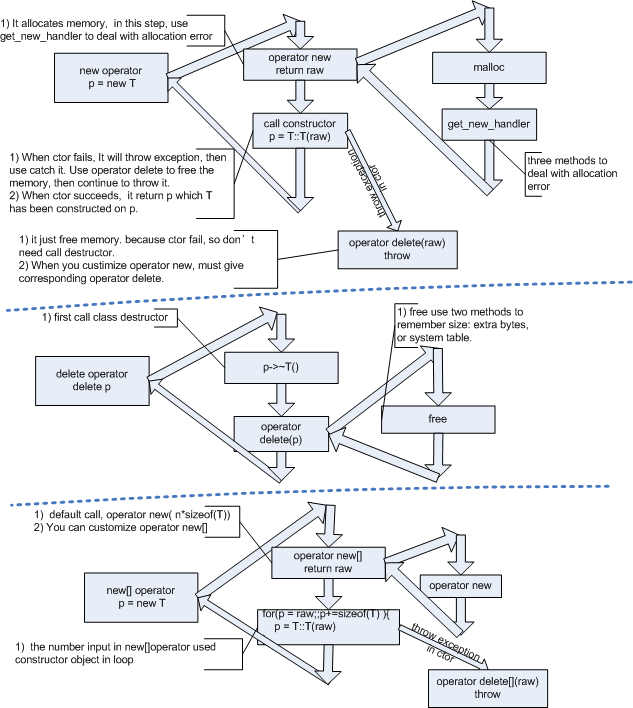
\includegraphics[width=0.90\linewidth]{pics/new.png}
	\caption{new operator and operator new.}
	\label{fig:smartpointer1}
\end{figure}


\chapter{Pointer and smart pointer}

\section{Raw pointer}

\begin{itemize}

    \item When do you use a smart pointer? Here I am changing this question to another question: When do you use a pointer? If you need a large array or memory resource, allocating it on the stack can cause a stack overflow. However, in practice, this requirement is deprecated because anytime you use array[] or new[], you should consider using \texttt{std::array}, \texttt{std::vector}, and \texttt{std::string} instead. Therefore, it's obsolete. Another usage is for polymorphism, but you can use a reference as well if it's just for polymorphism. Therefore, it's also obsolete.


	\item The only common usage of a pointer is to control the lifetime of the object that the pointer points to. For example, you may create the object in function 1 and delete it in function 4, so the object is neither stack duration nor static duration. You may or may not transfer ownership between functions, or you may want to create an object at runtime based on runtime conditions or user input (or decide not to create it). In other words, you need object (reference) semantics, not value semantics. One example is the observer pattern. The code below demonstrates the usage of a pointer, where the ToothBrush object needs to be controlled in terms of its lifetime and created dynamically.

\begin{lstlisting}[numbers=none]
class Person{
public:
	ToothBrush* pbrush;
	buyNewBrush(string &name){
	    if(pbrush != nullptr){
		    	delete pbrush;
	    }
	    if(name == "Orlab"){
	          pbrush = new Brush();
	    }
	}
	~Person(){
		if(pbrush != nullptr){
			delete pbrush;
	    }
    }
};
Person Yan();
Yan.buyNewBrush("Oralb");
//......Three months later...........
Yan.buyNewBrush("Philip");
}
\end{lstlisting}

	\item The problem with raw pointers includes buffer overrun, wild pointer, double delete, memory leak, no matching new and delete, and fragmentation of memory. To resolve buffer overrun and no matching new and delete issues, we can use \texttt{std::vector} and \texttt{std::string}. For resolving wild pointer, double delete, and memory leak issues, we can use smart pointers. With the help of smart pointers, the memory can be freed immediately, which is very important for performance. For example, if the memory looks like this: XXXOXXX, once we free O, we will have seven continuous memory. It not only frees up one byte of memory but also produces a larger chunk of memory for future allocation. This is critical in memory management.
	
	\item A raw pointer can be used as an alias of a variable. In C++, this kind of 'alias' semantic can also be achieved using a reference. A reference has two characteristics: it is non-null and cannot be changed. In other words, the top level of a const reference is default and cannot be changed. A reference always refers to the object with which it was initially initialized. This is why you have to initialize it. Unlike a pointer, a reference does not have a wild pointer problem. Therefore, there is no need to test if a reference is a null reference. However, if you have a reference to a local variable inside a function, when the function finishes, it can still have a dangling reference problem.
\begin{lstlisting}[numbers = none]
string &rs = s1;
rs = s2; //modified s1's value,rs still refer to s1
\end{lstlisting}	
	
	\item You can have a reference to a pointer, but a pointer to a reference is illegal. A reference is simply an alias to another object. You can't 'point' to a reference because it is not an object in itself, but merely another name for a real object. In terms of grammar, a reference to a reference has a different meaning and is called an rvalue reference.
\begin{lstlisting}[numbers=none]
int *p;
int *& rp = p; // reference to pointer is OK
int &* pr  //pointer to reference is ERROR

const int i = 12;
int& j = i; //ERROR, non-const reference can't refer to const object.
\end{lstlisting}	

	\item raw pointer has a little complicated relationship with array. There are two points to help you to understand:1) array name represent address; 2) address has type; 3)the same type address can be used to initialize the same type of pointer.   
\begin{lstlisting}
//char** ca = { "abc", "de" }; //Error
//char* ca[] = { {'a','b', 'c'} , {'d', 'e'} }; //Error
//char* ca[] = { "abc" , "de" }; //Error
//int** da = { {1,2,3}, {4,5} }; //Error
//int* da[] = { {1,2,3}, {4,5} }; //Error

int* da[] = { new int[] {1,2,3}, new int[] {4,5} };//array of pointer, ragged
int** pda = da;  // da is adress of pointer
cout << *(*(pda + 1) + 1) << endl;// output 5

int da1[2][3] = { {1,2,3}, {4,5,6} }; //an array of array, square
int(*pda1)[3] = da1;  //da1 is address of array [3]
cout << *(*(pda1 + 1) + 1) << endl;// output 5

char* ca[] = { new char[] {'a', 'b', 'c', '\0'}, new char[] {'d', '\0'} };
const char* cca[] = { "abc", "de" }; //here, char* cca[] doesn't work.
\end{lstlisting}
	\begin{enumerate}
		\item The square array is different with ragged array, Usually, we use pointer of array to simulate ragged array, and we use \texttt{a[2][3]} to denote the squared array.
		
		\item While the syntax for \texttt{((p+a)+b)} is the same, different types of \texttt{p} will result in different interpretations by the compiler. There is a difference between a pointer to a pointer and a pointer to an array.
		\begin{center}
			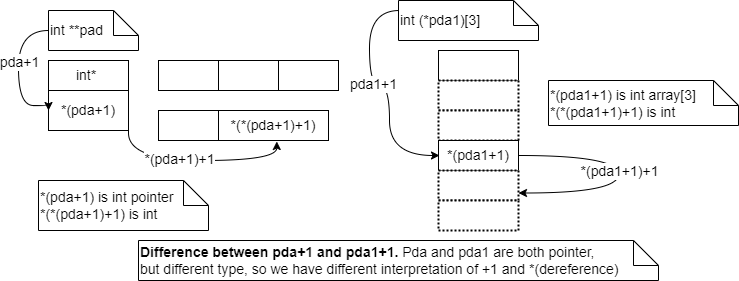
\includegraphics[width=0.9\linewidth]{pics/array.drawio}
		\end{center}
		
		\item \texttt{char*} is a little different, we can use "abc" to represent const char*, at the same time, we also need to add null charter in the end of char array.
		
	\end{enumerate}
	
\end{itemize}


\section{Basic smart pointer knowledge}

\subsection{Implementation smart pointer?}
\begin{itemize}

		\item "A simple \texttt{auto\_ptr} source code: You can learn how to overload \texttt{operator*()} and \texttt{operator->()}. Note that \texttt{auto\_ptr} has been deprecated in C++17, and the default value for smart pointers is \texttt{nullptr} if you do not initialize them. This helps you avoid the problem of wild pointers.
\begin{lstlisting}[frame=single, language=c++, mathescape=true]
template <class T> class auto_ptr{
    T* ptr;
public:
    explicit auto_ptr(T* p = 0) : ptr(p) {}
    ~auto_ptr()                 {delete ptr;}
    T& operator*()     {return *ptr;} //return reference 
    T* operator->()    {return ptr;} //interpret as (p.operator->())->m
};
\end{lstlisting}

	\item Four points when you want to implement smart pointer: All these design ideas can be used in other context, so you should know it. 

	\begin{enumerate}
		\item \texttt{operator *} and \texttt{operator ->} overload method.
		\item Disable copy and support move constructor for \texttt{unique\_ptr}
\begin{lstlisting}[frame=single, language=c++, mathescape=true]
unique_ptr(const unique_ptr&)    = delete;  
unique_ptr& operator=(const unique_ptr&)    = delete;
\end{lstlisting}

		\item For \texttt{shared\_ptr}, we need to pay attention to its reference number implementation. 
\begin{lstlisting}[frame=single, language=c++, mathescape=true]
class shared_count {
public:
	shared_count();
	void add_count();
	long reduce_count();
	long get_count() const;
	private:
	atomic_int use_count_;
};	
\end{lstlisting}		

\begin{lstlisting}[frame=single, language=c++, mathescape=true]
template <typename T>
class smart_ptr {
public:  
	...
private:  
	T* ptr_;  
	shared_count* shared_count_; //can't use shared_count or static shared_count
};	
\end{lstlisting}		
		
		
		\item template constructor. it is used to support assignment between child class smart pointer and parent class smart pointer.
		
\begin{lstlisting}[frame=single, language=c++, mathescape=true]
template <typename T>
class unique_ptr{
	.....
	template <typename U>  
	unique_ptr(unique_ptr<U>&& other)  {
		ptr_ = other.release();  
	}
}

unique_ptr<parent> pc{new Child};
unique_ptr<parent> pp{std::move(pc)};
\end{lstlisting}

	\end{enumerate}

\end{itemize}

\subsection{Why need smart pointer?}
\begin{itemize}
	
	\item "Just remember" is seldom the best solution! Therefore, we need smart pointers to perform the delete operator automatically when throwing an exception or returning in the middle of the code. If delete is not invoked at all, it can cause memory leaks. By using smart pointers, if an exception is thrown in the middle of a function, no memory leaks will occur. The most important thing is that smart pointers can manage exclusive or shared ownership automatically.


	\item There are four kinds of smart pointer: \texttt{auto\_ptr} \texttt{unique\_ptr} \texttt{shared\_ptr} and \texttt{weak\_ptr}  But only \texttt{unique\_ptr} , \texttt{shared\_ptr} and \texttt{weak\_ptr} are recommended to use. \texttt{auto\_ptr} is now deprecated, and should not be used in new code. When you get a chance, try doing a global search-and-replace of \texttt{auto\_ptr} to \texttt{unique\_ptr} in your code base.  \texttt{weak\_ptr} is mainly used for observer, you can always use raw pointer or reference for this purpose. Raw pointer can't check if pointee object is still valid, \texttt{weak\_ptr} can accomplish this task.


	\item Why is \texttt{auto\_ptr} not recommended? When you assign \texttt{targetP = sourceP}, it causes \texttt{sourceP} set to be \texttt{nullptr}. This can cause trouble when you use \texttt{sourceP} in the future. Additionally, you can't create containers that include \texttt{auto\_ptr}, as compiler will prohibit you from doing so!

\begin{lstlisting}[numbers=none]
auto_ptr<string> ps (new string("hello world") );
auto_ptr<string> ps1;
ps1 = ps;   // ps will be set null.
ps->size() // it will crash the application.

auto_ptr<string> parray[5]; //compiling error.
\end{lstlisting}

	
	\item When you construct a smart pointer, you must use 1) a pointer and 2) this pointer must be produced by new. You can't build a smart pointer by using the address operator, such as \texttt{unique\_ptr<double> ptr(\&int);}. Why? Because the smart pointer will call delete when it goes out of scope. The delete operator has to be used on a pointer produced by the new operator."

	
	\item A smart pointer supports flexible operations, such as obtaining the raw pointer \texttt{get}, relinquishing control of the pointed object \texttt{release}, and replacing the object it manages \texttt{reset}. A smart pointer also has a \texttt{bool} operator, which you can use to test if it's nullptr directly.

\begin{lstlisting}[numbers=none]
string * cp = new string("hello world");
shared_ptr<string> ps(cp);
string * cp1 = ps.get(); //use get() get normal pointer.

std::unique_ptr<int> ptr(new int(42));
if (ptr) std::cout <<  *ptr << '\n';
ptr.reset(); //
if (ptr) std::cout <<  *ptr << '\n';
\end{lstlisting}

	\item Combine smart pointer and \texttt{const}, we can have four different options. \texttt{shared\_ptr<T>} and \texttt{shared\_ptr<const T>} are not interchangeable. It goes one way - \texttt{shared\_ptr<T>} is convertable to \texttt{shared\_ptr<const T>} but not the reverse.
\begin{lstlisting}[numbers=none]
shared_ptr<T> p;        //---> T * p;
const shared_ptr<T> p;   //---> T * const p;
shared_ptr<const T> p;   //---> const T * p;
const shared_ptr<const T> p; //---> const T * const p;

shared_ptr<int> pint(new int(4)); // normal shared_ptr
shared_ptr<const int> pcint = pint;
 
shared_ptr<int> pint2 = pcint; // error! 
\end{lstlisting}


\end{itemize}

\subsection{unique\_ptr basic usage}
\begin{itemize}

\item Create \texttt{unique\_ptr} from new. \texttt{make\_unique} is better than inside new, inside new is better than outside new. let me explain it in below code.
\begin{lstlisting}[frame=single, language=c++]
string * cp = new string("hello world");

unique_ptr<string> ps = cp; // NOT allow to assign unique_ptr directly.
unique_ptr<string> ps (cp); //Ok, not good, new is outside of constructor.
unique_ptr<string> ps (new string("hello world")); //good , new is inside of constructor.
auto ps( std::make_unique<string>("hello") ); //best, make_unique 
\end{lstlisting}

\item Create \texttt{unique\_ptr} from another \texttt{unique\_ptr}, you have to use \texttt{std::move}.
\begin{lstlisting}[frame=single, language=c++]
unique_ptr<string> ps1 (new string("hello world"));

unique_ptr<string> ps2 ( ps1 ); //compile error
unique_ptr<string> ps2 ( std::move(ps1) ); //ok, ownership transfer from p1 to p2
unique_ptr<string> ps2 = std::move(ps1) ; //ok, nothing delete, p1 points to nullptr
\end{lstlisting}

\item When pass \texttt{unique\_ptr} value into a function.1) \textbf{For some exist \texttt{unique\_ptr}, use move to transfer ownership.} 2) \textbf{For new \texttt{unique\_ptr}, use \texttt{make\_unique} to assure exception safe.}	


\begin{lstlisting}[frame=single, language=c++]
void sink(unique_ptr<widget> arg1, unique_ptr<gadget> arg2); //functioni declaration

sink( std::move(exist_uptr_wi), std::move(exist_uptr_ga))
sink(make_unique<widget>(arg1, arg2),make_unique<gadget>(arg1, arg2));  
\end{lstlisting}


	\item Other \texttt{unique\_ptr} basic usages. 
\begin{lstlisting}[frame=single, language=c++]
auto ps1 (make_unique<string>("ps1"));
auto ps2 (make_unique<string>("ps2"));
ps1= ps2; //compile error, not allow copy
ps1 = std::move(ps2);  

ps1.reset(new string("ps3")); //pointer inside previous ps1 delete. 
string* pstr = ps1.release(); //reset and release 
\end{lstlisting}
\begin{description}
	\item[Line 4:]  Pointer inside previous \texttt{ps1} will be deleted. Pointer inside ps1 point to "ps2" string now. pointer inside \texttt{ps2} will set to nullptr.
	
	\item[Line 7:] Use \texttt{pstr} get pointer managed by \texttt{ps1}. Pointer in \texttt{ps1} will be set to \texttt{nullptr}. It's you duty to manage the memory which pointed by pointer \texttt{pstr}.
\end{description} 

	\item If a program attempts to assign one \texttt{unique\_ptr} to another. The compiler allows it if the source object is a temporary rvalue (It will call move constructor or assignment of \texttt{unique\_ptr} inside.) and disallows it if the source object has some duration. \textbf{It is a move-only type.} In another word, \texttt{unique\_ptr} supports \textbf{source and sink idiom}.
\begin{lstlisting}[numbers=none]
unique_ptr<string> ps2 = uqique_ptr<string>(new string("yo") ); //compile error

uqique_ptr<string> fun(){
	return unique_ptr<string> temp(new string("yan");
}
pu2 = fun(); //OK, support source

fun(unique_ptr up);  //use move to support sink
fun(move(other_up));
\end{lstlisting}

	\item Just observer, not transfer ownership , you can get pointer, or use \texttt{unique\_ptr} reference.
\begin{lstlisting}[numbers=none]
unique_ptr<string> ps1 (new string("ps1"));

fun(string* pstr);  //ps1.get()
fun(unique_ptr<string> & ref_ptr); // use unique_ptr reference.
\end{lstlisting}

	\item \texttt{Unique\_ptr} has new [] version. The existence of \texttt{std::unique\_ptr} for arrays should be of only intellectual interest to you, because \texttt{std::array}, \texttt{std::vector}, and \texttt{std::string} are virtually always better data structure choices than raw arrays. About the only situation I can conceive of when a \texttt{std::unique\_ptr<T[]>} would make sense would be when you're using a C-like API that returns a raw pointer to a heap array that you assume ownership of it.
\begin{lstlisting}[numbers=none]
unique_ptr<double []>  pda(new double[5] );// it will call delete [] inside.
\end{lstlisting}


    \item \texttt{unique\_ptr} can be used inside of class. Below class B disable value-copying (or to define a suitable copy-constructor  and operator= to handle it safely).
\begin{lstlisting}[numbers=none]
class B {  // this class can't be copy
public:
   unique_ptr<int> uni_ptr;
   B():uni_ptr(new int(0)) { }
};
\end{lstlisting}

    \item A common use for \texttt{std::unique\_ptr} is as a factory function return type for objects
in a hierarchy. Detail can be seen "effective modern c++ item 18". During construction, \texttt{std::unique\_ptr} objects can be configured to use custom deleters: arbitrary functions (or function objects, including those arising from lambda expressions) to be invoked when it's time for their resources to be destroyed. when a custom deleter can be implemented as either a function or a captureless lambda expression, the lambda is preferable. When a custom deleter is to be used, its type must be specified as the second type argument to \texttt{std::unique\_ptr}.

\begin{lstlisting}[frame=single, language=c++, mathescape=true]
template<typename... Ts>
auto makeInvestment(Ts&&... params) {
	
	auto delInvmt = [](Investment* pInvestment) {
		makeLogEntry(pInvestment); // makedelete
		delete pInvestment; // Investment
	};

	std::unique_ptr<Investment, decltype(delInvmt)> pInv(nullptr, delInvmt);
	
	if (...){
		pInv.reset(new Stock(std::forward<Ts>(params)...));
	}
	else if (... ) {
		pInv.reset(new Bond(std::forward<Ts>(params)...));
	}
	return pInv; // as before
}
\end{lstlisting}

    \item \texttt{std::unique\_ptr} is the C++11 way to express exclusive ownership, but one of its most attractive features is that it easily and efficiently converts to a \texttt{std::shared\_ptr}: This is a key part of why \texttt{std::unique\_ptr} is so well suited as a factory function return type. Factory functions can't know whether callers will want to use exclusive ownership semantics for the object they return or whether shared ownership
\begin{lstlisting}[frame=single, language=c++, mathescape=true]
shared_ptr<Investment> sp=makeInvestment(arguments); 
\end{lstlisting}


	\item If a vector contains \texttt{std::unique\_ptr<Fruit>} instead of raw pointers (to prevent memory leaks). vector need copy in and copy out. but \texttt{unique\_ptr} don't support copy. You can use below methods to resolve it. You can use \texttt{emplace\_back} with new pointer, but it will lead memory leak if extending vector size fail. A better method is to use unname \texttt{unique\_ptr.} The best method is to use \texttt{make\_unique}.

\begin{lstlisting}[frame=single, language=c++]
class Fruit { ... };
class Pear : Fruit { ... };
class Tomato : Fruit { ... };

std::vector<std::unique_ptr<Fruit> > m_fruits;
m_fruits.emplace_back(new Pear); //method 1, bad method
m_fruits.push_back(std::unique_ptr<Fruit>(new Pear)); //method2, good method
m_fruits.push_back(std::make_unique<Pear>());//method3, best method 
\end{lstlisting}

	\item You can sort \texttt{unique\_ptr} objects in an STL container as long as you do not use methods or algorithms that copy or assign one \texttt{unique\_ptr} to another, such as \texttt{copy()}. Refer to Item 8 in "Effective STL" for more information.

\begin{lstlisting}[numbers=none]
bool compare_by_uniqptr(const unique_ptr<SomeLargeData>& a,
                        const unique_ptr<SomeLargeData>& b) {
    return a->id < b->id;
}

sort(vec_uni.begin(),vec_uni.end(),compare_by_uniqptr);
\end{lstlisting}

\begin{lstlisting}[frame=single, language=c++]
typedef std::unique_ptr<int> unique_t;
typedef std::vector< unique_t > vector_t;

vector_t vec2(5, unique_t(new Foo));     //Error (Copy)
vector_t vec3(vec1.begin(), vec1.end()); //Error (Copy)
std::copy(vec1.begin(), vec1.end(), std::back_inserter(vec2)); // Error (copy)

vector_t vec3(make_move_iterator(vec1.begin()), make_move_iterator(vec1.end())); //Ok

std::sort(vec1.begin(), vec1.end()); //why sort is OK? 
\end{lstlisting}

\end{itemize}



\subsection{shared\_ptr basic usage}
\begin{itemize}
\item Every \texttt{shared\_ptr} has a control block inside of it. \textbf{When are control blocks created?} It's a very important concept to understand because it helps you better understand what happens when you create or assign a \texttt{shared\_ptr}.
\begin{center}
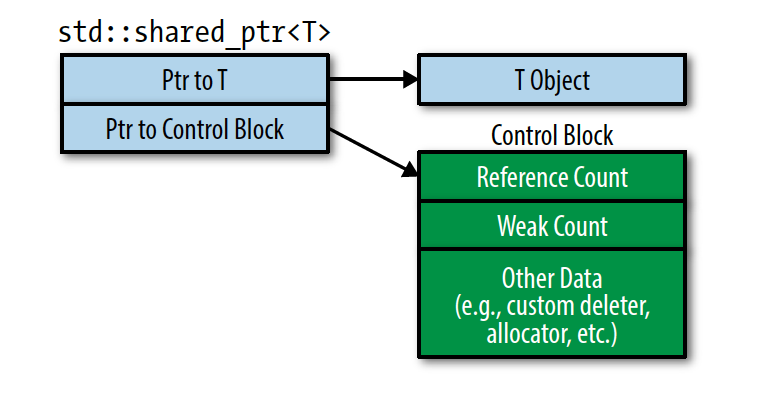
\includegraphics[scale=0.6]{pics/shared.png}
\end{center}


\begin{enumerate}
	\item \texttt{std::make\_shared}  always creates a control block. It manufactures a new object to point to, so there is certainly no control block for that object at the time \texttt{std::make\_shared} is called.
	
	\item A control block is created when a \texttt{std::shared\_ptr} is constructed from a unique-ownership pointer (i.e., a \texttt{std::unique\_ptr} ). As part of this construction, the \texttt{std::shared\_ptr} assumes ownership of the pointed-to object, and the unique-ownership pointer is set to nullptr.
	
	\item When a \texttt{std::shared\_ptr} constructor is called with a raw pointer, it creates a control block.
	
	\item When \texttt{std::shared\_ptr} constructors taking \texttt{std::shared\_ptrs} or \texttt{std::weak\_ptrs} as constructor arguments. it does \textbf{NOT} create new control blocks, because they can rely on the smart pointers passed to them to point to any necessary control blocks.
	
\end{enumerate}

	
    \item When \texttt{std::shared\_ptr} constructors take \texttt{std::shared\_ptrs} or \texttt{std::weak\_ptrs} as constructor arguments, they do \textbf{NOT} create new control blocks. Instead, they rely on the smart pointers passed to them to point to any necessary control blocks.
    
\begin{lstlisting}[frame=single, language=c++]
string * cp = new string("hello world");

shared_ptr<string> ps = cp; //NOT allow

shared_ptr<string> ps (cp); //outside new 
shared_ptr<string> ps1 (cp); //BAD!, that will cause UB.
shared_ptr<string> ps (new string("hello")); //inside new,good style
shared_ptr<string> ps( std::make_shared<string>("hello") ); //make, best style
\end{lstlisting}

	\item Some examples of creating \texttt{shared\_ptr} from another \texttt{shared\_ptr}.
\begin{lstlisting}[frame=single, language=c++, mathescape=true]
shared_ptr<string> ps1 (new string("hello world"));
shared_ptr<string> ps2 ( ps1 );  //refence count is 2 now, shared by ps1 and ps2
shared_ptr<string> ps2 ( move(ps1) );
\end{lstlisting}
\begin{description}
	\item[Line 3:] the original \texttt{ps1} will become nullptr, and the  refence count does not get modified. Just transfer refence count to \texttt{ps2}. 
\end{description}

    \item \texttt{shared\_ptr} assignment usage.
\begin{lstlisting}[frame=single, language=c++, mathescape=true]
shared_ptr<string> ps1 (new string("ps1"));
shared_ptr<string> ps2 (new string("ps2"));

ps1 = ps2;
ps1 = std::move(ps2);
ps1.reset(cp); 
\end{lstlisting}
\begin{description}
	\item[Line 4:] Use assignment  1) In \texttt{ps1}, previous reference count decrements 1. (If equal 0, it will delete) 2) \texttt{ps1} points to current reference count 3) and current reference count increments 1
	
	\item[Line 5:] Use move 1) In \texttt{ps1}, previous reference count decrements 1. (If equal 0, it will delete) 2) \texttt{ps1} points to current reference count 3) \texttt{ps2} is null now. 
	
	\item[Line 6:] Use \texttt{reset}. pointer inside previous \texttt{ps1} will decrement 1. by now, current \texttt{ps1} reference count will be 1.
\end{description}

\item Difference between constructor and assignment.
\begin{enumerate}
	\item When assignment, previous decrements 1 and current increment 1;
	\item When copy constructor, current increment 1;
	\item When constructor from raw pointer, current is 1;
\end{enumerate}

\begin{center}
	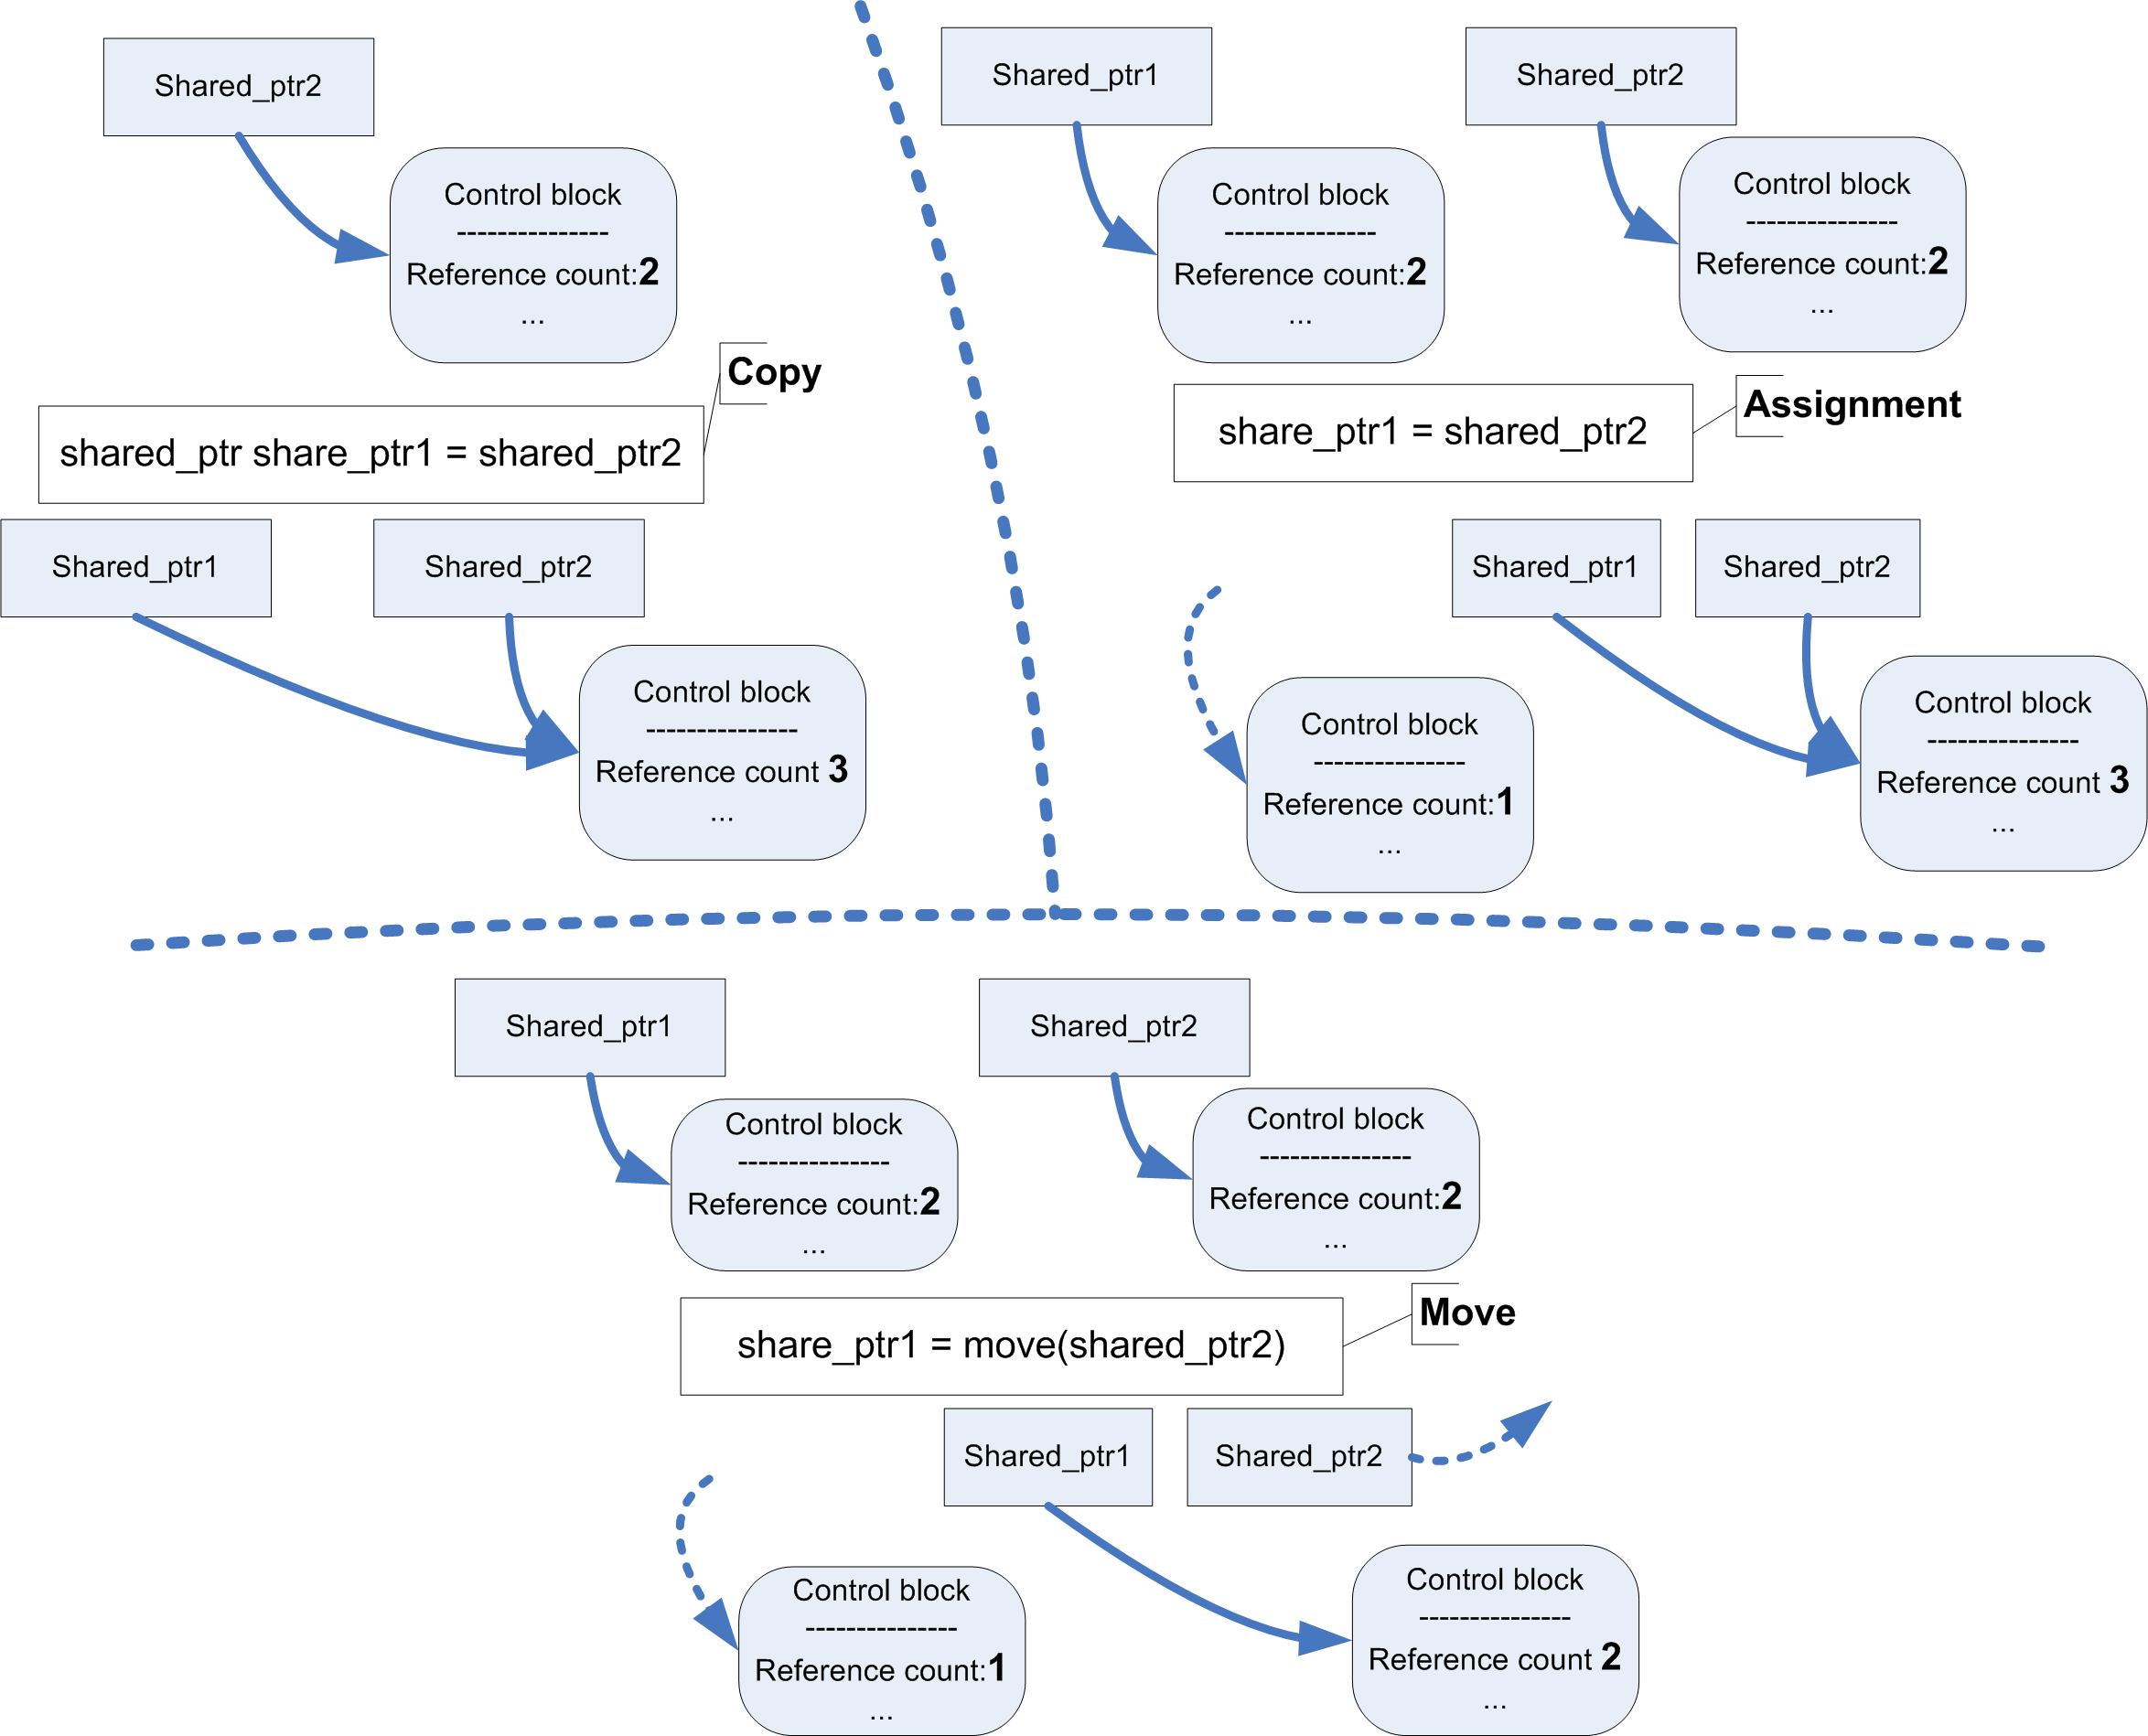
\includegraphics[width=0.9\linewidth]{pics/shared_ptr.png}
\end{center}


\item Just observer, not transfer or share ownership , you can get pointer, or use \texttt{shared\_ptr} reference. 
\begin{lstlisting}[numbers = none]
shared_ptr<string> ps1 (new string("ps1"));

fun(string* pstr);
fun(shared_ptr<string>& ref_ptr);
\end{lstlisting}



	\item Usage of \texttt{enable\_shared\_from}. If you don't use it, multiple distinct \texttt{shared\_ptr} objects with separate reference counts. For this reason you must never create more than one \texttt{shared\_ptr} \textbf{from the same raw pointer.} It has become C++11 standard.
\begin{lstlisting}[frame=single, language=c++]
class Test : public boost::enable_shared_from_this<Test> {
public:
    boost::shared_ptr<Test> GetObject(){
        return shared_from_this();  //correct way.
        //return shared_ptr<test>(this); //wrong way, from the same raw pointer.
    }
};
int main(int argc, char *argv[]){
    boost::shared_ptr<Test> p( new Test( ));
    boost::shared_ptr<Test> q = p->GetObject();
}
\end{lstlisting}

	\item The basic implementation of \texttt{enable\_shared\_this}. It uses CRTP design pattern and I will introduce CRTP design pattern in OOP chapter.  When we construct \texttt{shared\_ptr}, if the type is inherit from \texttt{enable\_shared\_this}, then we initialize \texttt{weak\_this}. 
\begin{lstlisting}[frame=single, language=c++]
template<class T>
class enable_shared_from_this {
	mutable weak_ptr<T> weak_this;
public:
	shared_ptr<T> shared_from_this() {
		return shared_ptr<T>(weak_this); 
	}
}
\end{lstlisting}

\end{itemize}


\subsection{weak\_ptr basic usage}
\begin{itemize}

    \item The relationship between \texttt{weak\_ptr} and \texttt{shared\_ptr} begins at birth. \texttt{std::weak\_ptrs} are typically created from \texttt{std::shared\_ptrs}. You can only create a \texttt{weak\_ptr} out of a \texttt{shared\_ptr} or another \texttt{weak\_ptr}. A truly smart pointer would deal with this problem by tracking when it dangles, i.e., when the object it is supposed to point to no longer exists. That's precisely the kind of smart pointer \texttt{std::weak\_ptr} is. \textbf{You can't test if a raw pointer is dangle or not.}

    \item \texttt{std::weak\_ptrs} can't be dereferenced, nor can they be tested for nullness. That's because \texttt{std::weak\_ptr} isn't a standalone smart pointer. It's an augmentation of \texttt{std::shared\_ptr}. Almost the only things you can do are to interrogate it to see if the managed object is still there, or construct a \texttt{shared\_ptr} from it.

\begin{lstlisting}[frame=single, language=c++,mathescape=true]
auto spw = std::make_shared<Widget>(); //reference count is 1
std::weak_ptr<Widget> wpw(spw);  //reference count remains 1
...
if (wpw.expired())
\end{lstlisting}

    \item The \texttt{lock()} method creates a new \texttt{std::shared\_ptr} that shares ownership of the managed object. If there is no managed object, the \texttt{shared\_ptr} returned by the method is empty.

\begin{lstlisting}
std::shared_ptr<Widget> spw1 = wpw.lock(); //if wpw's expired, spw1 is null
auto spw2 = wpw.lock(); //same as above, but uses auto
std::shared_ptr<Widget> spw3(wpw); //if wpw expired, throw std::bad_weak_ptr.
\end{lstlisting}

    \item Potential use cases for \texttt{std::weak\_ptr} includes: caching, observer lists, and the prevention of \texttt{std::shared\_ptr} cycles.  All the detail can be seen in "Effective Modern ++" Item 20.
\begin{lstlisting}[frame=single, language=c++]
std::shared_ptr<const Widget> fastLoadWidget(WidgetID id){
	static std::unordered_map<WidgetID, std::weak_ptr<const Widget>> cache;
	auto objPtr = cache[id].lock();

	if (!objPtr) { // if not in cache,
		objPtr = loadWidget(id); // load it
		cache[id] = objPtr; // cache it
	}
	return objPtr;
}
\end{lstlisting}
\begin{description}
	\item[Line 5:] objPtr is \texttt{std::shared\_ptr} to cached object . (or null if object's not in cache). For above requirement, you also can use raw pointer, But for raw pointer, you can't detect if original one has been delete. 
\end{description}

    \item An example of \texttt{shared\_ptr} cyclic dependency problem. Below code has memory leak. \texttt(A) and \texttt{B} doesn't have chance to call destructor.
\begin{lstlisting}[]
class B;
class A {
    shared_ptr<B> sP1; // use weak_ptr instead to avoid CD
public:
    A() {  cout << "A()" << endl; }
    ~A() { cout << "~A()" << endl; }
    void setShared(shared_ptr<B>& p) {
        sP1 = p;
    }
};
class B {
    shared_ptr<A> sP1;
public:
    B() {  cout << "B()" << endl; }
    ~B() { cout << "~B()" << endl; }
    void setShared(shared_ptr<A>& p) {
        sP1 = p;
    }
};
int main() {
    shared_ptr<A> aPtr(new A);
    shared_ptr<B> bPtr(new B);
    aPtr->setShared(bPtr);
    bPtr->setShared(aPtr);
}
\end{lstlisting}

\end{itemize}


\subsection{make function}

\begin{itemize}
	\item Never use the new operator directly in C++14! Instead, prefer using the make function. However, if you need a custom deleter or are adopting a raw pointer from elsewhere, you should avoid using \texttt{make\_unique}. Also note that \texttt{make\_unique} was only introduced in C++14. This function perfect-forwards its parameters to the constructor of the object being created, then constructs a \texttt{std::unique\_ptr} from the raw pointer that new produces, and finally returns the created \texttt{std::unique\_ptr}.
	
	\item \texttt{std::make\_unique} and \texttt{std::make\_shared} are two of the three make functions: functions that take an arbitrary set of arguments, perfect-forward them to the constructor for a dynamically allocated object, and return a smart pointer to that object. The third make function is \texttt{std::allocate\_shared}
	
	\item make function has tree advantage: simply, exception safety and allocate once for efficiency.
	
	\begin{enumerate}
		\item The new operator requires repeating the type being created, whereas the make functions do not. That's why using the make functions is generally better than using new. For a comparison, see the source code below.
		
\begin{lstlisting}[frame=single, language=c++, mathescape=true]
auto upw1(std::make_unique<Widget>()); // better
std::unique_ptr<Widget> upw2(new Widget); 
		
auto spw1(std::make_shared<Widget>()); // better
std::shared_ptr<Widget> spw2(new Widget); 
\end{lstlisting}
		
		\item The second reason to prefer make functions has to do with exception safety. More explanation can be found in "More effective C++" item 21. 
		
		\item The third reason is allocation efficiency. Every \texttt{std::shared\_ptr} points to a control block that contains the reference count for the pointed-to object. When using \texttt{std::make\_shared}, a single chunk of memory is allocated to hold both the Widget object and the control block. If we don't use \texttt{make\_shared}, we would have to perform two separate allocation actions.
		
	\end{enumerate}
	
	\item make function has its limitation:
	\begin{enumerate}
		\item For example, none of the make functions permit the specification of custom deleter.
		
		\item the perfect forwarding code uses parentheses, not braces. The bad news is that if you want to construct your pointed-to object using a braced initializer, you must use new directly. Using a make function would require the ability to perfect-forward a braced initializer, but, as "Effeictive Modern C++"Item 30 explains, braced initializers can't be perfect-forwarded.
\begin{lstlisting}
template<typename T>
void f(T para);

f({1,2,3}) //error, can't deduce type T

template<typename T>
void f(std::initializer_list<T> initList);
f({1,2,3}) //OK.
\end{lstlisting}

\begin{lstlisting}
auto upv = std::make_unique<std::vector<int>>(10, 20); //10 elements. 
auto initList = { 10, 20 }; //create std::initializer_list
auto spv = std::make_shared<std::vector<int>>(initList);
\end{lstlisting}
\begin{description}
	\item[Line 3:] create \texttt{std::vector} using \texttt{std::initializer\_list} constructor. You need to build \texttt{initializer\_list} variable outside of \texttt{make\_shared}. 
\end{description}
		
		\item As long as \texttt{std::weak\_ptrs} refer to a control block (i.e., the weak count is greater than zero), that control block must continue to exist. And as long as a control block exists, the memory containing it must remain allocated. The memory allocated by a \texttt{std::shared\_ptr} make function, then, can't be deallocated until the last \texttt{std::shared\_ptr} and the last \texttt{std::weak\_ptr} referring to it have been destroyed
	\end{enumerate}
	
	\item If you can't use make function, you have to create \texttt{shared\_ptr} first, then pass it to function, but a better way is to move it.
\begin{lstlisting}[frame=single, language=c++]
std::shared_ptr<Widget> spw(new Widget, cusDel);
processWidget(spw, computePriority()); // correct, but not optimal; 

processWidget(std::move(spw),computePriority());  // both efficient and exception safe
\end{lstlisting}

	\item Guideline: Use \texttt{make\_unique} to create an object that is not shared (at least not yet), unless you need a custom deleter or are adopting a raw pointer from elsewhere.
	
\end{itemize}

\subsection{wrapping non-pointer resource in smart pointer}

\subsubsection{Customize deleter in unique\_ptr and shared\_ptr}

\begin{itemize}
		\item Both \texttt{std::unique\_ptr} and \texttt{std::shared\_ptr} use delete as its default resource-destruction mechanism, but it also supports custom deleters. Deleter type is part of \texttt{unique\_ptr} type. Deleter type is not part of \texttt{shared\_ptr} type. \texttt{shared\_ptr} use type erase technique, which is introduced in "Generic programming" section.
\begin{lstlisting}[frame=single, language=c++]
auto loggingDel = [](Widget *pw){ // custom deleter
	makeLogEntry(pw);
	delete pw;
};

std::unique_ptr< Widget, decltype(loggingDel) > upw(new Widget, loggingDel);
std::shared_ptr<Widget> spw(new Widget, loggingDel);		
\end{lstlisting}
	
%	  \item \texttt{unique\_ptr} can input another deleter type. 
%\begin{lstlisting}[frame=single, language=c++, mathescape=true]
%template<class T, class Deleter = std::default_delete<T>> 
%class unique_ptr;
%
%template<typename T, typename D, bool Empty = std::is_empty_v<D>>
%class unique_ptr{
%	T* ptr;
%	D d;
%	...
%};
%
%template<typename T, typename D>
%class unique_ptr<T, D, true> : D{
%	T* ptr;
%	...
%};	
%\end{lstlisting}	
	

	\item \texttt{unique\_ptr} can input another deleter type. Below is a few kind of deleter and their size comparison.
	\begin{enumerate}
		\item std::function - heavy stuff, on 64 bit, gcc it showed me 40 bytes.
		
		\item Function pointer - it’s just a pointer, so now \texttt{unique\_ptr} contains two pointers: for the object and for that function… so 2*sizeof(ptr) = 8 or 16 bytes.
		
		\item \textbf{Stateless functor (and also stateless lambda)} - it’s actually very tricky thing. You would probably say: two pointers… but it’s not. Thanks to empty base optimization - EBO the final size is just a size of one pointer, so the smallest possible thing.
		
		\item State-full functor or Lambda - if there is some state inside the functor then we cannot do any optimizations, so it will be the size of ptr + sizeof(functor)
	\end{enumerate}

	\item For stateless functors or lambdas, the size is just one pointer, which means we don't need to pay a space fee. That's why \texttt{unique\_ptr} has two template parameters, and one of them allows you to specify the deleter type. If the deleter type is an empty stateless functor, the size will be just one pointer. If you don't care about space, but value flexibility (e.g., you want to pass any caller-callable object), you can always add your own type erasure on top by using \texttt{std::function}. For example, you can have \texttt{unique\_ptr<T, std::function<void(T*)>>}.
		
\begin{lstlisting}[frame=single, language=c++]
typedef struct {
	//...
} Foo;

Foo* createObject(int i_val, double d_val) {
	Foo* output = (Foo*)malloc(sizeof(Foo));
	return output;
}
struct FooDeleter {
	void operator()(Foo* p) const {
		destroy(p);
	}
};
	
using FooWrapper = std::unique_ptr<Foo, FooDeleter>;
FooWrapper foo(createObject(32, 3.14));
\end{lstlisting}

	\item The \texttt{std::shared\_ptr} template has only one parameter though: the type of the pointee. But you can use a custom deleter with this one too, even though the deleter type is not in the class template. \textbf{shared\_ptr and std::functions use type erase technology.} you can see the type erase technology in generic programming chapter later.
\begin{lstlisting}
template< class T > class shared_ptr;
\end{lstlisting}
	
	\item Part of the reason is that \texttt{shared\_ptr} needs an explicit control block anyway for the ref count and sticking a deleter in isn't that big a deal on top. \texttt{unique\_ptr} however doesn't require any additional overhead, and adding it would be unpopular- it's supposed to be a zero-overhead class. \texttt{unique\_ptr} is supposed to be static. 
\begin{lstlisting}[frame=single, language=c++]
typedef struct {
	//...
} Foo;

Foo* createObject(int i_val, double d_val) {
	Foo* output = (Foo*)malloc(sizeof(Foo));
	return output;
}

void destroy(Foo* obj) {
	free(obj);
}

std::shared_ptr<Foo> foo(createObject(32, 3.14), destroy);
\end{lstlisting}

	\item In order to correctly use \texttt{shared\_ptr} with an array, you must supply a custom deleter. But we don't recommend using \texttt{shared\_ptr} with array. \textbf{Any time you new a array, you should first consider using STL container directly.}
\begin{lstlisting}[numbers=none]
template< typename T >
struct array_deleter {
	void operator ()( T const * p){
		delete[] p;
	}
};

shared_ptr<int> sp(new int[10],array_deleter<int>());	
\end{lstlisting}


	
		\item Based on the previous introduction about customized deleters, we can manage \texttt{FILE*} with smart pointers using the source semantic of \texttt{unique\_ptr}.
\begin{lstlisting}[frame=single, language=c++]
struct FILEDeleter {
	void operator()(FILE *pFile){
		if (pFile)
		fclose(pFile);
	}
};
using FILE_unique_ptr = unique_ptr<FILE, FILEDeleter>;

FILE_unique_ptr make_fopen(const char* fname, const char* mode){
	FILE *fileHandle= nullptr;
	auto err = fopen_s(&fileHandle , fname, mode);  
	return FILE_unique_ptr(fileHandle); 
}

FILE_unique_ptr pFilePtr = make_fopen("test.txt", "rb"); //no need to call fclose
\end{lstlisting}		
		
		\item Just the same idea, if you want to use \texttt{shared\_ptr} wrap \texttt{FILE*}, see below example.
\begin{lstlisting}[frame=single, language=c++]
using FILE_shared_ptr = std::shared_ptr<FILE>;

FILE_shared_ptr make_fopen_shared(const char* fname, const char* mode){
	FILE *fileHandle = nullptr;
	auto err = fopen_s(&fileHandle, fname, mode);
	return FILE_shared_ptr(fileHandle, FILEDeleter()); // FILEDeleter() is variable, not type
}	
\end{lstlisting}		
		
		\item For \texttt{fstream}, it is different from \texttt{FILE*} as it uses value semantics and implements RAII. If you need to share ownership, you can pass a reference directly since it does not support copying.
		
\begin{lstlisting}[numbers=none]
fp = fstream(name,mode)};
setLogFile(ifstrea& );
setLogFile(fp);
\end{lstlisting}

	
%		\item For \texttt{unique\_ptr}, if you can deduct pointer type from deleter, \texttt{unique\_ptr} will use it directly, so you just know SC\_HANDLE is a kind of "pointer", but you don't know exact type, you can write just like below.  That is because in \texttt{unique\_ptr}, If you provide and deleter and inside deleter, you also provide pointer type. If that type exists, we use this as resource type, otherwise \texttt{T*}. Must satisfy NullablePointer.
%
%\begin{lstlisting}[frame=single, language=c++]
%struct SvcHandleDeleter{
%	typedef SC_HANDLE pointer; //define pointer type here
%	SvcHandleDeleter() {};
%	
%	void operator()(pointer h) const {
%		CloseServiceHandle(h);
%	}
%};
%	
%typedef std::unique_ptr<SC_HANDLE,SvcHandleDeleter> unique_sch;
%//you define pointer in side the deleter, so we use SC_HANDLE, not SC_HANDLE* 
%	
%unique_sch scm(::OpenSCManagerA(0, 0, SC_MANAGER_ALL_ACCESS));
%\end{lstlisting}
%	
%	\item For shared pointer, type-erasure makes it impossible with the current interface to achieve exactly what type you want. So you can use a dumb way, Just like a pointer to pointer. If you don't know what is behind SC\_HANDLE. 
%	
%\begin{lstlisting}[frame=single, language=c++]
%std::shared_ptr<SC_HANDLE> sp(new SC_HANDLE(
%              ::OpenSCManagerA(0, 0, SC_MANAGER_ALL_ACCESS)),
%	[](SC_HANDLE* p){ ::CloseServiceHandle(*p); delete p; });
%\end{lstlisting}
%
%		\item Different with previous example, if you know \textbf{HANDLE in windows is just void* type pointer}, so you can use this way to deal with windows handle. it will save you a lot of trouble. 
%	
%\begin{lstlisting}[frame=single, language=c++]
%struct HANDLEDeleter{
%	void operator()(HANDLE handle) const{
%		if (handle != INVALID_HANDLE_VALUE)
%		CloseHandle(handle);
%	}
%};
%	
%using HANDLE_unique_ptr=unique_ptr<void, HANDLEDeleter>;
%	
%HANDLE_unique_ptr make_HANDLE_unique_ptr(HANDLE handle){ ...
%	return HANDLE_unique_ptr(handle);
%}
%	
%auto hInputFile = make_HANDLE_unique_ptr(
%                            CreateFile(strIn, GENERIC_READ, ...));
%\end{lstlisting}
	
	\item Use \texttt{shared\_ptr} to wrap a handle, A good introduction is "Making a HANDLE RAII-compliant using \texttt{shared\_ptr} with a custom deleter" in stackoverflow

\end{itemize}
	
\section{Smart pointer usage}
\subsection{smart pointer and polymorphism}

\subsubsection{pointer\_cast function}
\begin{itemize}
	\item The basic idea is that smart pointer base and smart pointer derived are not covariant at all. This is similar to how vector<Base> and vector<Derived> work. Even \texttt{DerivedClass} inherit \texttt{BaseClass,}  You can't cast \texttt{shared\_ptr<DerivedClass>} to \newline 
	\texttt{shared\_ptr<BaseClass>} because there is no inheritance relationship between the types. 
	
	\item The \texttt{shared\_ptr<T>(const shared\_ptr<Y>\&)} constructor doesn't help because it is only usable if Y* is implicitly convertible to T*, i.e. it is there to support the same pointer conversions as would happen implicitly, like \texttt{DerivedClass*} to \texttt{BaseClass*,} not \texttt{BaseClass*} to \texttt{DerivedClass*}. That is why we need \texttt{static\_pointer\_cast}.
\begin{lstlisting}
template< class T, class U > 
std::shared_ptr<T> static_pointer_cast( const std::shared_ptr<U>& r ) noexcept {
    auto p = static_cast<typename std::shared_ptr<T>::element_type*>(r.get());
    return std::shared_ptr<T>{r, p};
}
\end{lstlisting}
\begin{description}
	\item[Line 4:] That is called Aliasing \texttt{shared\_ptr} constructor, detail can be google "std::shared\_ptr's secret constructor"
\end{description}

	\item An example of \texttt{static\_pointer\_cast} is below:
\begin{lstlisting}
struct BaseClass {};

struct DerivedClass : BaseClass {
	void f() const {
		std::cout << "Sample word!\n";
	}
};

int main() {
	std::shared_ptr<BaseClass> ptr_to_base(make_shared<DerivedClass>());
	std::static_pointer_cast<DerivedClass>(ptr_to_base)->f();
	std::dynamic_pointer_cast<DerivedClass>(ptr_to_base)->f();
	static_cast<DerivedClass*>(ptr_to_base.get())->f(); //Error
}
\end{lstlisting}

\end{itemize}

\subsubsection{Four casts in polymorphism}
\begin{itemize}
\item In this section, you need to know four types of smart pointer casting.
\begin{enumerate}
\item \texttt{share\_ptr} child to base;
\item \texttt{share\_ptr} base to child (down cast);
\item \texttt{unique\_ptr} child to base;
\item \texttt{unique\_ptr} base to child (down cast);
\end{enumerate}

		\item For \texttt{shared\_ptr}, it support derived to base \texttt{shared\_ptr} copy or assignment. Behind the hood, you need to know the template member function. Detail can be found in effective C++ item 45 "Use member function templates to accept "all compatible types". Why you can? because it get raw pointer and wrapped it again and compiler allow it.

		\item  For \texttt{shared\_ptr} base, you can't assign it to the \texttt{shared\_ptr} child, so you must use \\ \texttt{static\_pointer\_cast} and \texttt{dynamic\_pointer\_cast}. They only support \texttt{shared\_ptr}. They use \texttt{shared\_ptr} aliasing constructor, get raw pointer, use static or dynamic cast, then build derived \texttt{shared\_ptr} too. Detail can be found: \\
			"std::static\_pointer\_cast vs static\_cast<std::shared\_ptr<A > >"

		\item If you don't want to shared ownership, but just want to be a observer, you can use reference, but for \texttt{shared\_ptr} base reference, You have to use const. Why do we need const?
	
\begin{lstlisting}[frame=single, language=c++, mathescape=true]
void doSomething(const std::shared_ptr<Base>& ptr) {
    std::cout<<ptr.use_count()<<std::endl; 
}

std::shared_ptr<Derived1> pd1 = std::make_shared<Derived1>();
//doSomething(pd1);  Will not compile here.
doSomething(shared_ptr<Base> temp(pd1));
doSomething(static_pointer_cast<Base>(pd1));
\end{lstlisting}
	\begin{description}
	\item[Line 7:] from pd1 build temporary base \texttt{shared\_ptr} pointer.
	\item[Line 8:] \texttt{static\_pointer\_cast} also return a temporary base \texttt{shared\_ptr}. That is why you need \texttt{const} in line 1
\end{description}


	\item The static cast can also be used for checking downcasts, but it checks at compile time and may sometimes fail. Unlike the dynamic cast, which checks at run time and requires the class to have at least one virtual function. More details about this can be found in the second chapter. The basic idea is similar to the distinction between \texttt{static\_cast} and \texttt{dynamic\_cast}.

	\item For \texttt{unique\_ptr}, You can use move from derived pointer to base pointer directly.
\begin{lstlisting}[frame=single, language=c++, mathescape=true]
void doSomething(const std::unique_ptr<Base> ptr) {
    ptr->run();
}

int main() {
    std::unique_ptr<Derived1> pd1 = std::make_unique<Derived1>();
    doSomething(std::move(pd1));
}
\end{lstlisting}

	\item For down cast \texttt{unique\_ptr}, There are no counter part of \texttt{static\_pointer\_cast}. So only way you can do is use release and wrap it again.

\begin{lstlisting}[frame=single, language=c++, mathescape=true]
template<typename TO, typename FROM>
unique_ptr<TO> static_unique_pointer_cast (unique_ptr<FROM>&& old){
	return unique_ptr<TO>{static_cast<TO*>(old.release())};
	//conversion: unique_ptr<FROM>->FROM*->TO*->unique_ptr<TO>
}

unique_ptr<Base> foo = fooFactory();
unique_ptr<Derived> foo2 = 
              static_unique_pointer_cast<Derived>(std::move(foo));
\end{lstlisting}

	\item For const reference, there are three methods: 1) Use move 2) Change function interface 3) Change parameter.
\begin{lstlisting}[frame=single, language=c++, mathescape=true]
void f(const unique_ptr<Base>& base)

unique_ptr<Derived> derived = unique_ptr<Derived>(new Derived);
f(derived); //this fail;

f(std::move(derived)); //method 1 work, Why?
    //because int i = 3; const float& dr = i; compile OK
                       
void f(std::unique_ptr<Derived> const&); //method 2, Change function interface

std::unique_ptr<base> derived = std::make_unique<Derived>();//method 3, Change parameter.
std::unique_ptr<base> derived(new Derived);
\end{lstlisting}


	\item There are three places where you can use smart pointers: in a braced scope (function), as a class member, and as a container item. In these three places, you can have exclusive ownership, shared ownership, or observer semantics. In the next two sections, I will mainly discuss the relationship between smart pointers and classes and the relationship between smart pointers and functions.

\end{itemize}


\subsection{Smart pointer and Semantic of RAII}

\begin{itemize}
	
	\item The basic idea of RAII is to wrap a resource in a local object, in other words, to represent a resource using a local object. RAII objects acquire resources in their constructors and release them in their destructors to avoid resource leaks.
		
\begin{lstlisting}[numbers = none]
//C version,
File* fp = fopen("/path/to/file");
// throw exception here, then resource leaking
fclose(fp); //this statement will not be executed. 
	
fun{ //c++ version
	fstream if("path/to/file")
	if.getline()
	// you don't need to if.close().
}

std::unique_ptr<FILE, int(*)(FILE*)>  //smart point implement RAII
myFile( fopen("myfile", "rb"), fclose );              
\end{lstlisting}
\begin{description}
	\item[Line 12] use smart pointer to wrap FILE* in C language. the custom deleter type is function pointer. The deleter function is: \texttt{fclose()} 
\end{description}


	\item Wrapping a pointer into a RAII class. Why do you use raw pointer? Maybe you need some customized action in runtime, or use handle is only method to use this resource or any other reason. And this time, you have to write your own destructor to release the resource.
\begin{lstlisting}[numbers=none]
class RAII_Class {
	~RAII_Class(){//release m_resource here}
private:
	Resource* m_resource;
	
};	
\end{lstlisting}

	\item When implementing RAII, be conscious of copy construction and assignment. The compiler-generated version probably won't be correct because it will cause two pointers or handles to refer to the same resource, which is absolutely a bad smell in code. Therefore:
\begin{enumerate}
	\item If it's not copyable, use \texttt{=delete} on copy constructor. \texttt{std::unique\_ptr} is a good example of this idea.
	
	\item If it's copyable value member, duplicate the resource and follow the 'Rule of Five'.Both \texttt{std::vector} and \texttt{std::string} are good examples of this idea.
\begin{lstlisting}[numbers=none]
Class RAII_Class{
	RAII_Class(const RAII_Class& rhs){
		m_resource = new Resource( *(rhs.m_resource));
	}
	
	RAII_Class(RAII_Class&& rhs){
		m_resource = rhs.m_resource;
		rhs.m_resource = nullptr;
	}
private:
	Resource* m_resource;
}		
\end{lstlisting}
	
	\item If it's copyable reference value, recommend to use \texttt{shared\_ptr} to manage it's lifetime to avoid 1) memory leak and 2) dangling pointer. 
\end{enumerate}
			
	\item Whenever you're dealing with a resource that requires paired acquire/release function calls, it's best to encapsulate that resource in an object. Examples of such resources include fopen/fclose, lock/unlock, and new/delete. It's important to consider resources generically, such as a pointer \texttt{*p} pointing to a new object or a handle to a file. We can wrap a handle to a file into an ifstream, and wrap a pointer *p into a smart pointer. Another example is when you're working with the WinAPI; in that case, you can use a RAII semantic class. In other words, don't only think of a pointer that points to an object in memory as a resource; resource is a generic concept. In multithreaded programming, a thread is also a type of resource, so we have the \texttt{jthread}, which is also a RAII semantic class. Similarly, a mutex is a resource, so we have the \texttt{lock\_guard}, which is also a RAII semantic class. You can think \texttt{lock\_guard} as a smart mutex which wraps mutex, just like \texttt{unique\_ptr} is a smart pointer which wraps raw pinter. 
\begin{lstlisting}[numbers=none]
class module {
public:
	explicit module(std::wstring const& name)
	: handle { ::LoadLibrary(name.c_str()) } {}
	
	~module{
	::FreeLibrary();
	}
private:
	HMODULE handle;
};
\end{lstlisting}


	\item Smart pointers in C++ are good examples of RAII, but they go further. \texttt{std::unique\_ptr} denotes exclusive ownership by deleting its copy constructor at the syntax level, while \texttt{std::shared\_ptr} represents shared ownership by maintaining a reference count. In other words, smart pointers are not only RAII classes, but they also represent two different types of ownership.

	\item Next, I would like to talk about some common patterns of using RAII classes when defining your own class. You can use an RAII member or use a smart pointer to wrap resources in your own classes. When using a smart pointer, you want to express different ownership semantics. First and foremost, it's not recommended to use raw pointers directly unless you have strong reason.

	\begin{enumerate}
		\item Use RAII member, In this way, you don't need to build destructor manually.
\begin{lstlisting}[]
class Foo{
private:
	string m_str; // RAII class
	vector<int> m_vc; //RAII class
};
\end{lstlisting}
			
				\begin{enumerate}
					\item RAII class and your own class have same life duration.
					
					\item \texttt{m\_str} and \texttt{m\_vc} are value semantic, so there is no ownership concern and is copyable(\texttt{Foo f2 = f1;}) and can move with efficiency(\texttt{Foo f1 = Foo();} ). 
					
					\item If all members are RAII classes (have it's own copy and move special function), You don't need to write any special function in your class(Foo). Just follow the "Rule of Zero".
				\end{enumerate}
					
	\item Use smart point to wrap pointers or handles;
\begin{lstlisting}[numbers=none]
class RAII_Container {
private:
	unique_ptr<string>  m_str;
	vector<unique_ptr<int> > vc;
};
		\end{lstlisting}
\begin{enumerate}
	
		\item  When you wrap handle, you can custom this delete behavior. See source code below:
\begin{lstlisting}[numbers=none]
class module {
public:
	explicit module(std::wstring const& name)
	: handle { ::LoadLibrary(name.c_str()) } {}
private:
	using module_handle=std::unique_ptr<
			void,decltype(&::FreeLibrary)>;
	module_handle handle;
};
\end{lstlisting}
	\item For \texttt{unique\_ptr}, it has the following characteristics: 1) the same lifetime as the owning object, 2) exclusive ownership and not copyable by default, and 3) supports move operations. You can still follow the "rule of zero," meaning that you don't provide any customized special member functions, and the class will not be copyable. However, if you build a copy constructor yourself, obtain a raw pointer from the original object, and construct a new \texttt{unique\_ptr} member from the original object's raw pointer, you can make the class copyable.

	\item For \texttt{shared\_ptr}; 1) Not same lifetime 2) shared ownership, 3) copyable and moveable. When you move a \texttt{shared\_ptr}, origin one is set to nullptr and ref count doesn't increase.  You can still follow "rule of zero".and resource will be deleted when ref count is 0.
	
\begin{lstlisting}[numbers=none]
class Student{
	shared_ptr<SchoolBus> pBus;
}				
\end{lstlisting}
			
\end{enumerate}

	\end{enumerate}

		
		\item  Next, I would like to give two special cases. For example, suppose I want to design a Car class where people can customize its engine, and it should support copying. In this context, your Car class should use raw pointers because: 1) value semantic members don't support customization (dynamic changes), and 2) \texttt{unique\_ptr} doesn't support copying. Therefore, you have to use \texttt{Engine *pEn} and follow the "Rule of Five."
\begin{lstlisting}[numbers=none]
class Car{
	Engine *pEn; //follow "Rule of Five"
	~Car(){delete pEn} // assure RAII
}
\end{lstlisting}
		
	\item For some other non-copyable contexts, such as: 1) a Person class where the semantics require non-copyability, 2) situations where performance is a consideration, such as with the Big class {int [30000];}, and 3) situations where the implementation constrains copying, such as with the iostream class. In such contexts, you can use \texttt{unique\_ptr} to manage resources and make them uncopyable.
\begin{lstlisting}[numbers=none]
class Person{
    uniqu_ptr<Resource> pRes;
}
\end{lstlisting}
		
	\item In summary, Design your class according to semantics. Don't use it just because syntax supports it. Use it because it can better represent relationships and constraints in real life.
	
\end{itemize}



\subsection{Smart pointer and function}
\subsubsection{Function interface design}

\begin{itemize}

    \item \textbf{Inside a function}

\begin{enumerate}
    \item If you don't want to create dynamically or large array, don't use new. Just use local auto object. Even you need large array, consider STL container first.

    \item When you have to use new, and this function has \textbf{Ownership of pointer, means that they have the same life duration},  use \texttt{unique\_ptr}. In this way, you don't need delete and it's exception safe.
\end{enumerate}
\begin{lstlisting}
fun(){
	Foo fo(1,2); //It makes obj directly, when you don't need dynamic.
	
	if(input == "Foo")
		uniqu_ptr<Foo> up(new Foo(1,2) ); //use new, then smart pointer wrap it.
}
\end{lstlisting}

    \item \textbf{Arguments of a function.}

\begin{enumerate}

    \item Passing \texttt{unique\_ptr} by reference is for in/out \texttt{unique\_ptr} parameters. When the function is supposed to actually accept an existing \texttt{unique\_ptr} and potentially modify it to refer to a different object. 

    \item \texttt{const unique\_ptr} \& MUST be observer. So another way is to use raw pointer as observer directly, or use \texttt{std::weak\_ptr}. 

    \item If you want to transfer ownership to callee from caller, use \texttt{uniqu\_ptr}, and use move. Passing \texttt{unique\_ptr} by value means "sink."

    \item If you want to shared ownership to callee from caller, use \texttt{shared\_ptr}.

    \item Use a non-const \texttt{shared\_ptr\&} parameter only to modify the \texttt{shared\_ptr}. Use a \texttt{const shared\_ptr\&} as a parameter only if you're not sure whether or not you'll take a copy and share ownership; otherwise use \texttt{widget*} instead (or if not nullable, a \texttt{widget\&)}.

    \item When you assign \texttt{unique\_ptr} to \texttt{shared\_ptr}, use move.
\end{enumerate}

\begin{lstlisting}[frame=single, language=c++]
Foo *fo = new Foo();  //bad smell here.
fun(Foo * p);
delete fo;

fun(Foo &p); //use reference to improve efficiency

uniqu_ptr<Foo> up(new Foo() );
fun(uniqu_ptr<Foo>& up); //use reference, can't copy 

fun(uniqu_ptr<Foo> down);  //prototype
fun(std::move(up) );

std::unique_ptr<std::string> unique = 
			std::make_unique<std::string>("test");
			
std::shared_ptr<std::string> shared = 
			std::move(unique);
\end{lstlisting}


\item \textbf{Return from function.}
\begin{enumerate}

    \item Don't  use reference refer to a local object created inside of fun.

    \item If you have to use New, and you want to transfer Ownership from callee to caller. return \texttt{unique\_ptr}.

    \item If there is no clear single owner, store and return \texttt{shared\_ptr}. (in below example, caller of fun() is single owner, so use \texttt{unique\_ptr})

\begin{lstlisting}[numbers=none]
Foo* fun(){   //old c style.
	return new Foo();
}

unique_ptr<Foo> fun(){  // this is better.
........
	return unique_ptr<Foo>(new Foo()) ;
}
\end{lstlisting}

\item Below use \texttt{shared\_ptr}, because \texttt{Server} is public used, and no single owner.
\begin{lstlisting}[numbers=none]
shared_ptr<Server> buildNewServer(){  // this is better.
	return shared_ptr<Server>(new Server()) ;
}

shared_ptr<Server> serverForClass1 = buildNewServer();
shared_ptr<Server> serverForClass2  = serverForClass1;
\end{lstlisting}

\end{enumerate}

    \item About smart pointer and function interface. There is a good article. "GotW \#91 Solution: Smart Pointer Parameters"
\end{itemize}

\section{Smart pointer summary}

\subsection{Difference between value and reference semantic}
\begin{itemize}
	\item A type has value semantics if the object's observable state is functionally distinct from all other objects of that type. This means that if you copy an object, you have a new object, and modifications of the new object will not be in any way visible from the old object. In C++, all primitive type are value semantic. such as \texttt{bool/int/double/char}. The container in STL, such as (\texttt{std::pair}, \texttt{std::vector}, \texttt{std::string}, \texttt{std::map}) are also value semantic. If a type wishes to have value semantics, and it needs to store objects that are dynamically allocated, then on copy operations, the type will need to allocate new copies of those objects. It must also do this for copy assignment. This kind of copying is called a "deep copy". Advantage of value semantic is easier lifetime management. They must be stack object, A member of other object or element in a container.
	
	\item On the contrary, reference(object) semantic does not copy a object, such as a people object, it's not right to copy a people object from other people object. A type is said to have reference semantics if an instance of that type can share its observable state with another object (external to it), such that manipulating one object will cause the state to change within another object. C++ pointers have value semantics with regard to which object they point to, but they have reference semantics with regard to the state of the object they point to. Usually, for reference semantic class, we should delete its copy constructor. Reference semantic can't be copy, but you can use pointer or reference to refer to it. All smart pointers are value semantic, not reference(object) semantic. We should never define a smart pointer like below:
\begin{lstlisting}[numbers=none]
shared_ptr<Foo>* pFoo = new shared_ptr<Foo>(new Foo); //Wrong semantic.
\end{lstlisting}	
	
	\item When we just want to express reference semantic, smart pointer is also much better than raw pointer. Below code demonstrates how to use smart pointer to express reference semantic.
	
\begin{lstlisting}[frame=single, language=c++, mathescape=true]
typedef shared_ptr<Parent> ParentPtr;

class Child : boost::noncopyable{
	explicit Child(const ParentPtr& myDad_) :myParent(myDad__){}
	..
private:
	weak_ptr<Parent> myParent;
}; 

typedef shared_ptr<Child> ChildPtr;
class Parent: public enable_shared_from_this<Parent>, private boost::noncopyable{
  	void addChild(){
  		myChild.reset(new Child(shared_from_this()));
  	}
private:
	ChildPtr myChild;
};
--------------------------------
ParentPtr p(new parent);
p->addChild(); //Child is created by parent.
\end{lstlisting}
\begin{enumerate}
	\item First, we should not use raw pointer to refer to each other, it's reference semantic, you can't know if the object which you refer is still valid.
	
	\item Then, you can't use two \texttt{shared\_ptrs} here. otherwise, it will cause cyclic reference.
	
	\item Then, you have to use one shared\_ptr and one \texttt{weak\_ptr}. Usually, owner(parent) has \texttt{shared\_ptr}, the counter part(child) has \texttt{weak\_ptr}. 
	
	\item \texttt{weak\_ptr} must use \texttt{shared\_ptr} to initialize. 
	
	\item Then we have problem here, you can't use this here, because it is raw pointer, a trick here is use \texttt{shared\_from\_this}.
\end{enumerate}

	
	
\end{itemize}

\subsection{Smart pointer usage suggestions}

\begin{itemize}
	
	\item Instead of using C FILE* and char* as strings, it's better to use the fstream class and string object. This is because fstream and string are exception-safe and provide better type safety and memory management compared to FILE* and char*. 

	\item In smart pointer implementation, we have used a few common C++ language characteristics. We use optimized base class empty in \texttt{unique\_ptr}, we use type erase in \texttt{shared\_ptr}, we also used CRTP in \texttt{enable\_from\_this}. They are interesting and worth learning and apply them in your future project. 

	\item You must ensure that there is only one manager object for each managed object. You do this by writing your code so that when an object is first created, it is immediately given to a \texttt{shared\_ptr} to manage, and any other \texttt{shared\_ptrs} or \texttt{weak\_ptrs} that are needed to point to that object are all directly or indirectly copied or assigned from that first \texttt{shared\_ptr}. The customary way to ensure this is to write the new object expression as the argument for a \texttt{shared\_ptr} constructor, or use the \texttt{make\_shared} function. Sometimes, factory methods returns a plain pointer to the object they create. in this case however, the callee still should generally be immediately assigning this returned object to a \texttt{shared\_ptr} or \texttt{unique\_ptr}.  Methods should return a plain-pointers when it is up to the caller to handle ownership of the object(exclusive ownership or shared ownership).


	\item Methods can take plain-pointers as their arguments for just observe it. Or use smart pointer to transfer or get ownership.
\begin{lstlisting}[frame=single, language=c++]
ObserveFun(Foo* p);
ObserveFun(smart_pointer.get() );
ObserveFun(unique_ptr<Foo> &p); //Just observer.

UniqueFun(unique_ptr<Foo> p);  //exclusive ownership
UniqueFun(make_unique_ptr<Foo>(new Foo() )); //get ownership
UniqueFun(move(other_unique_ptr) )  //transfer ownership

SharedFun(shared_ptr<Foo> p);
\end{lstlisting}

	\item If you want to get the full benefit of smart pointers, your code should avoid using raw pointers to refer to the same objects; otherwise it is too easy to have problems with \textbf{dangling pointers and double deletions}. In particular, smart pointers have a get() function that returns the pointer member variable as a built-in pointer value. This function is rarely needed. As much as possible, leave the built-in pointers inside the smart pointers and use only the smart pointers.

	\item vector of raw pointer is not good design, there are two problems. The first question is that you don't know if raw pointer is still valid? The second is that when you use remove algorithm on vector or raw pointer, it will cause memory leak. Detail can be found in "effective STL" item 33 and 7. If we use vector of smart pointer, we can resolve both of these questions.  

	\item Observer pointers are pointers which do not keep the pointed object alive. Raw pointers are bad when used for performing manual memory management, i.e. new and delete. When used purely as a means to achieve reference semantics and pass around non-owning, observing pointers, there is nothing intrinsically dangerous in raw pointers. Just not to dereference a dangling pointer. A better option is to use \texttt{weak\_ptr}, provided that you have \texttt{shared\_ptr} already.

\begin{lstlisting}[frame=single, language=c++]
observe(subject * s1)
observe(weak_ptr<subject> wptr) //no owner and life time policy with weak_ptr
\end{lstlisting}

\item When using smart pointer, consider three policies of smart pointer usage:
\begin{enumerate}
	\item \textbf{Ownership policy:} use smart pointer.
	\item \textbf{Observer Policy:} use raw pointer, reference or \texttt{weak\_ptr}. Prefer to use \texttt{weak\_ptr}.
	\item \textbf{Nullity Policy:} Not allow nullptr, prefer to use reference. Prefer reference than pointer.
\end{enumerate}

\begin{lstlisting}
class Man{
	Heart t_ ; //same life time span
	unique_ptr<Brush> pbrush_;  //exclusive ownership, 
	shared_ptr<Woman> pwife_; //shared ownership
	weak_ptr<Company> pcom_;  //observer
	Woman& mother;  //Nullity
	void getMoney(const Bank&);
}	
\end{lstlisting}

\begin{figure}[h!]
	\centering
	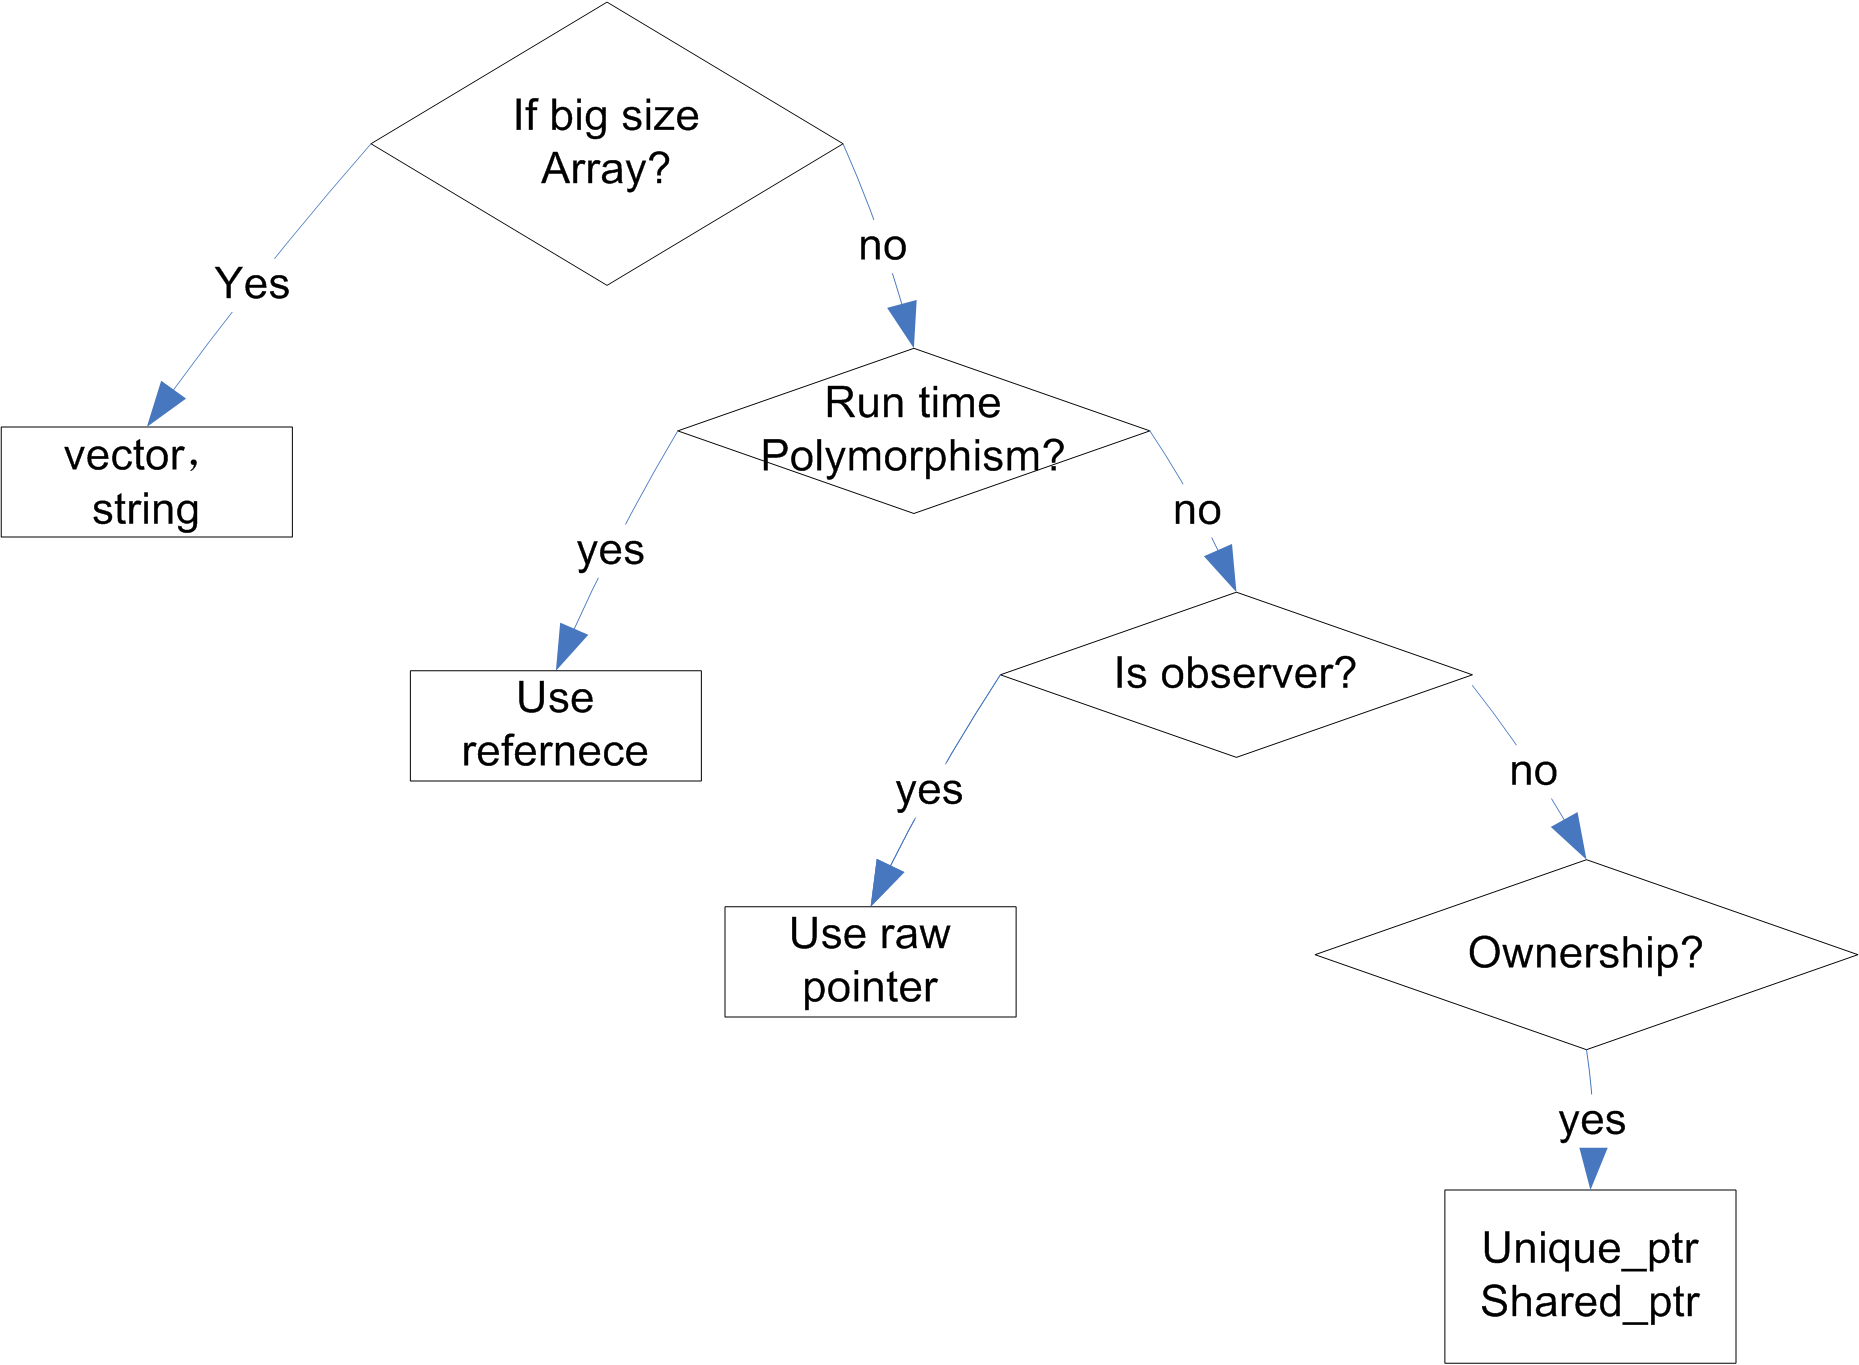
\includegraphics[width=0.75\linewidth]{pics/smartPointer.png}
	\caption{When to use smart pointer?}
	\label{fig:smartpointer}
\end{figure}
\end{itemize}

\chapter{lvalue reference and rvalue reference}

\section{Prequel-before rvalue reference }
\subsection{lvalue, rvalue and value category}
\begin{itemize}

	\item Each C++ expression, which could be an operator with its operands, a literal, a variable name, or any other construct, is characterized by two independent properties: type and value category. Every expression has a certain type, such as the expression 1+2 having the \texttt{int} type. Usually, the index operator [] returns a reference type, and \texttt{std::move} returns an rvalue reference type. Furthermore, each expression belongs to exactly one of the three primary value categories: lvalue, prvalue, and xvalue. We will introduce xvalue later.
				
    \item The value categories of an expression determine two important but separate properties. Firstly, they determine whether the expression has an identity, which means it refers to an object with a variable name, even if the name is not explicitly used in the expression. In other words, the compiler needs to know which expressions can legally appear on either side of an assignment statement. For example, \texttt{5=x;} is an illegal statement in C++. Secondly, the value categories determine whether it is legal to implicitly move the expression's value. Specifically, they determine whether the expression, when used as a function parameter, will bind to r-value parameter types or not.

	\item The definition of lvalue as 'something that can be put on the left side of =' is not entirely accurate. This is because even though \texttt{const int a} is also an lvalue, you cannot put 'a' on the left side of =. Instead, an lvalue is characterized by three properties:
\begin{enumerate}
	\item\textbf{lvalue has identity}, (can get address by \& operator),
	\item \textbf{lvalue can be persist beyond the expression. }
	\item \textbf{lvalue can be copied, can't be moved,} because you need to keep original one intact.
\end{enumerate}
\begin{lstlisting}
"abc" //lvalue, string literal is an lvalue.
int a{}; //name varabile 
int& foo();
foo(); //lvalue, function return reference.
++a; //prefix operator
*(p+1); //dereference of pointer
f.a // if f is lvalue.	
\end{lstlisting}

	\item On the contrary, prvalue has no \textbf{identity}, and will not \textbf{persist} beyond expression and should be moved for certain resource type object for high efficiency.
\begin{lstlisting}
42    // literal below are all rvalue.
int foo();  
foo(); //function call return value
a+b;   //result of arithmetic
&a //address 
satic_cast<double> a //casting and return temporary
a++; //postfix operator
double{}; //tempory variable	
\end{lstlisting}

	\item Remember that any expression that evaluates to an lvalue reference (e.g., a function call, an overloaded assignment operator, etc.) is an lvalue. Any expression that returns an object by value is an rvalue.

\begin{lstlisting}[frame=single, language=c++, mathescape=true]
string& lvalue_fun();
lvalue_fun(); 
lvalue_fun() = "hello"; //OK, return value persist.
&lvalue_fun();          //OK, can get address because it has identity

string pvalue_fun();
pvalue_fun(); 
pvalue_fun() = "hello"; //ERROR, no persist.
&pvalue_fun();          //ERROR, no identity 	
\end{lstlisting}

	\item Why doesn't an rvalue persist in C++? One reason is that rvalues are stored differently from lvalues, giving the compiler more freedom to optimize code for better performance. Specifically, a value can be stored in a register of the CPU and never actually be in memory, which means it has no address. While it's not certain, this is likely one of the main reasons why we cannot get the address of an rvalue. Additionally, since an rvalue is semantically temporary, it's more likely to be stored in temporary places or optimized in a way that makes it difficult to map to an address. Even if it can be mapped, it would be counterproductive in terms of performance.
\end{itemize}

\subsection{lvalue reference}
\begin{itemize}
	\item Why do we need to introduce reference in C++? In C++ 98, we introduce reference because some operating overloading functions are simply impossible to perform without reference.
\begin{lstlisting}
struct integer { 
	integer(int v) : value(v) {}
	int value; 
};
void operator++(integer i) { // This doesn't actually modify i
	i.value++;
}
// This is ill-formed and won't compile -already an operator++ for integer*
void operator++(integer* i) { 
	*i.value++;
}

void operator++(integer& i) {  //only this option work.
	i.value++;
}
\end{lstlisting}

	\item Later, we introduce const lvalue reference to "materialize" a rvalue(temporary). 
\begin{lstlisting}
//integer(2)+integer(3) doesn't work with below function.
integer operator+(integer& i1, integer& i2) {
	return integer(i1.value + i2.value);
}

//integer(2)+integer(3) works with const reference.
integer operator+(const integer& i1, const integer& i2) {
	return integer(i1.value + i2.value);  //i1 and i2 is xvalue here.
}	
\end{lstlisting}

	\item  In another word, only lvalue can bind to reference to \texttt{non-const}. Only \texttt{const} reference can bind to temporary and prolong temporary variable(rvalue) life. Only stack-base \texttt{const} reference can work in this way. If a \texttt{const} reference is class member, it can't work in this way. \texttt{const} reference bound to rvalue is used in copy constructor widely before C++11 (case 3 in below code snippet).
\begin{lstlisting}[frame=single, language=c++]
Foo f(){ //case 1:
	return obj;
}
const Foo & rf = f(); //const reference bind to temporary.

class Foo{ // case 2, 
	Foo(int i);  //Foo constructor
}
f(const Foo & crf); //function declaration
f(1); //from 1 build a temp Foo object, and const reference can bind it.

class Foo{ //case 3,
	Foo(const Foo & foo); //without const, line 15 will fail.
}
Foo f3 = f1+f2; //f1+f2 is rvalue	
\end{lstlisting}

     

%\item A \texttt{const} object reference passed into a function, if you want to return it , it must be \texttt{const} too. Usually, It has no any practical meanings when you do in this way. 
%\begin{lstlisting}[numbers=none]
%const int &fun(const int& i){ 
%	return i;
%}
%//or const_cast 
%int &fun(const int& i){ 
%	return const_cast<int&>(i);
%}
%\end{lstlisting}


	\item Rvalues denote temporaries or objects that act like temporaries. What's special about temporaries is that they are used in a limited way: their value will be read once and then they will be destroyed. This observation is useful in implementing move semantics. So, what is move semantics? It doesn't really move a large amount of data; instead, it moves an index of data, much like moving a file in a hard disk. If your class allocates a lot of resources, you should implement a copy constructor to avoid shallow copying. However, for some rvalues, performing an expensive copy is unnecessary because the temporary variable will disappear and doesn't need to be kept intact. This is where a new type is introduced to distinguish lvalues from rvalues and take different actions: for lvalues, we copy, and for rvalues, we move.
\begin{lstlisting}[numbers=none]
Foo::Foo(const Foo & rhs){
	while(ptr++;)
		ptr[i] = foo.ptr[i]  //expensive copy
}

Foo foo1 = foo2; //foo2 is lvalue, we have to copy
Foo foo1 = foo2+foo3; //foo2+foo3 is rvalue, can move to improve effecience. 
Foo foo1 = getFoo(); //rvalue, same
\end{lstlisting}  	

\end{itemize}

%\subsection{lvalue reference overload}
%\begin{itemize}
%		\item Reference type will not decide overload resolution.
%\begin{lstlisting}[numbers=none]
%void foo(int x)  { std::cout << "foo(int)"   << std::endl; }
%void foo(int& x) { std::cout << "foo(int &)" << std::endl; }
%
%int i = 42;
%int &j = i;
%foo(i);  //ambiguous call
%foo(j);  //ambiguous call, event j is reference type.
%\end{lstlisting}
%
%		\item \texttt{const} will not help to distinguish value and reference type.
%\begin{lstlisting}[numbers=none]
%void foo(int x)  { std::cout << "foo(int)"   << std::endl; }
%void foo(const int& x) { std::cout << "foo(cons int &)" << std::endl; }
%
%int i = 42;
%const int &j = i;
%foo(i); // ambigous call
%\end{lstlisting}
%
%	\item \texttt{const} will help to distinguish between reference type.
%\begin{lstlisting}[numbers=none]
%void foo(int &x)  { std::cout << "foo(int&)"   << std::endl; }
%void foo(const int& x) { std::cout << "foo(cons int &)" << std::endl; }
%	
%int i = 42;
%const int &j = i;
%foo(j); // call const version
%\end{lstlisting}
%
%
%		\item lvalue reference can only bound to lvalue, so we can use value category, help us to pick up the right function.
%\begin{lstlisting}[numbers=none]
%void foo(int x)  { std::cout << "foo(int)"   << std::endl; }
%void foo(int& x) { std::cout << "foo(int &)" << std::endl; }
%
%foo(2);	 //call foo(int x),2 is prvalue, so int& can't matches
%\end{lstlisting}
%
%\begin{lstlisting}[numbers=none]
%void foo(int x)  { std::cout << "foo(int)"   << std::endl; }
%void foo(int& x) { std::cout << "foo(int &)" << std::endl; }
%void foo(const int& x) { std::cout << "foo(cons int &)" << std::endl; }
%	
%foo(2);	 //ambious, 2 is prvalue, so const int & and int both match
%\end{lstlisting}
%
%\item summary:
%\begin{enumerate}
%	\item Given lvalue, reference type and value type produce ambiguous call.
%	\item Given lvalue, constness can't help distinguish reference type and value type.
%	\item Given const lvalue, constness help to distinguish const reference type and lvalue reference type.
%	\item both value and const lvalue reference can match rvalue, but lvalue reference can not. 
%\end{enumerate}
%\begin{center}
%	\begin{tabular}{|c|c|c|c|}
%		\hline
%		& value & lvalue reference  & const lvalue reference  \\
%		\hline
%		lvalue & OK &  OK & OK  \\
%		\hline
%		rvalue & OK & Not & OK   \\
%		\hline
%	\end{tabular}
%\end{center}
%
%\end{itemize}

\section{rvalue reference and move semantic}

\begin{itemize}
	
	\item We usually use type as the overload resolution method. For reference types, we can use the value category as an overload resolution method too. For example, before C++11, rvalues only matched const lvalue references; they would not match lvalue references. However, const lvalue reference has a problem: const reference can bind both lvalue and rvalue, so we can't distinguish when to move or when to copy. This is an efficiency problem that we can't change. For rvalues, we sometimes don't want to perform an expensive copy; we want to perform a cheap move instead. That is why we need a new kind of reference type. Once we have such a new reference type, we can allow a function to branch at compile-time (via overload resolution) on the condition "Am I being called on an lvalue or an rvalue?" There are two requirements for the new reference type: it should only bind to rvalue, and we should be able to change it. In the below code, what should "????" be? Although \texttt{foo2} and \texttt{foo2+foo3} have the same type, they have different value categories (one is lvalue and the other is rvalue). That is why we invented rvalue references in C++11, which can only bind to rvalues.

\begin{lstlisting}[frame=single, language=c++]
Foo::Foo(const Foo & rhs){ //copy constructor
	while(ptr++;)
	    ptr[i] = rhs.ptr[i]  //expensive copy
}	

Foo::Foo(???? rhs){  //move constructor
	ptr = rhs.ptr;  //efficient move(steal)
	rhs.ptr = nullptr;
}	
	
Foo foo1 = foo2;  //use the first copy constructor
Foo foo1 = foo2+foo3;  //for right value, use move constructor
Foo foo1 = getFoo();  //same as previous line.
\end{lstlisting}

\begin{center}
		\begin{tabular}{|c|c|c|}
			\tophline 
			type & which value category can bind & changable \\
			\tophline 
			lvalue reference & lvalue(non-const)  &  Yes  \\
			\tophline  
			rvalue reference &  rvalue(non-const)&  Yes \\
			\tophline 
			const lvalue reference & lvalue or rvalue(const or non-const) & No  \bottomhline 
		\end{tabular} 
\end{center}

	\item If \texttt{X} is any type, then \texttt{X\&\&} is called an rvalue reference to \texttt{X}, that is compound type in C++. For better distinction, the ordinary reference \texttt{X\&} is now also called an lvalue reference. Rvalue references will implicitly bind to rvalues and to temporaries that are the result of an implicit conversion. i.e. Below is well formed because float is implicitly convertible to int; the reference would be to a temporary that is the result of the conversion.
\begin{lstlisting}
float f = 0f; 
int&& i = f;  //int&& is rvalue reference, an bind to temporary variable.
\end{lstlisting}
	
	\item Rvalue references can be used to extend the lifetimes of temporary objects (note, lvalue references to const can extend the lifetimes of temporary objects too, but they are not modifiable through them):
	
\begin{lstlisting}[frame=single, language=c++, mathescape=true]
std::string s1 = "Test";
std::string&& r1 = s1; //ERROR rvalue reference can't bind to lvalue.
		
const std::string& r2 = s1 + s1;//lvalue reference to const extends lifetime. 
r2+="test" //Error  can't modify through reference to const.
		
std::string&& r3 = s1 + s1; //rvalue reference extends lifetime
r3 += "Test"; //can modify through reference to non-const.                   
\end{lstlisting}
	 
	
	\item An example code for move constructor and move assignment.	Don't declare objects \texttt{const} if you want to be able to move from them. Move requests on \texttt{const} objects are silently transformed into copy operations.
	
\begin{lstlisting}[numbers=none]
Foo::Foo(const Foo & rhs){
	while(ptr++;)
	  ptr[i] = rhs.ptr[i]  //expensive copy
}
Foo::Foo(Foo&& rhs){ //no const here
	ptr = rhs.ptr;  //efficient move(steal)
	rhs.ptr = nullptr;
}
Foo& Foo::operator=(Foo&& rhs){
	delete[] ptr;
	ptr = rhs.ptr;  //efficient move(steal)
	rhs.ptr = nullptr;
	return *this;
}
\end{lstlisting}
	
	\begin{enumerate}
		\item Move constructor will not move resource automatically, you need to coding it by your self. You can't move in normal constructor. because, It must keep origin obj intact.  You can steal when \texttt{Foo(f1+f2)}, but when you used \texttt{Foo(f1)}.  It will destroy \texttt{f1}. Without  move constructor, normal copy constructor will treat \texttt{Foo f = f1+f2} and \texttt{Foo f = f1} the same way.
		
		\item With move copy constructor, normal copy constructor deal with \texttt{Foo f = f1}, and move copy constructor deal with \texttt{Foo f = f1+f2}, for \texttt{f1+f2}, you can steal resource, because nobody need to use \texttt{f1+f2} later any more. In move constructor, always set \texttt{rhs.ptr = nullptr}; And no \texttt{const} qualifier in move constructor and move assignment parameter.
		
	\end{enumerate}
	
%	\item In below examples, Foo obj1=obj2+obj3. if you don't have move constructor, In operator + function, a temp obj is produced,  and when operator+ function return, another temp obj temp2 is produced .  Then in the end, objtemp2 is passed to ctor,  So, ctor is called three times. and copy content is also called three times.
%	
%\begin{lstlisting}[numbers=none]
%	Foo Foo::operator+( const Foo & f) const {
%			Foo temp = Foo(n+f.n);
%			//copy happen here.
%			return temp;
%		}
%		
%		Foo obj1=obj2+obj3  
%		// three constructor called without move ctor
%	\end{lstlisting}
%	
%	\item If you have move constructor. In operator + function, a temp objtemp1 is produced,  When return objtemp1, It will not produce objtemp2. (because objtemp1 is rvalue.) then objtemp1 is passed to move ctor. In side move ctor, the resource address has been move to new obj1.  Just one temp objtemp1 and one actual copy happen. ( just new pointer = old pointer; and old pointer = NULL).

\end{itemize}

\section{xvalue}
\begin{itemize}
	\item In this section, there are three important points:1) \texttt{std::move} and why do we need a new value type--xvalue? 2) Academic definition of xvalue and some practical expressions which are xvalue. 3) Relationship between xvalue and rvalue reference.
\end{itemize}

\subsection{std::move function and xvalue}

\begin{itemize}
	
	\item C++11 allows you to use move semantics not just on rvalues, but, at your discretion, on lvalues as well. An good example is swap function, here if you can move lvalue, the efficiency will be better. 
	
\begin{lstlisting}[numbers=none]
template<class T> 
void swap(T& a, T& b) { 
	T tmp(std::move(a));
	a = std::move(b);  //std::move must return rvalue.
	b = std::move(tmp);
} 
\end{lstlisting}
	
	\item By now, \texttt{std::move} must return rvalue, How? If \texttt{std::move} return value? \texttt{std::move(b)} is rvalue, but not good. Because it means that we have to copy input variable once inside \texttt{std::move}, then return the copied one. If \texttt{std::move} return  lvalue reference? \texttt{std::move(b)} is lvalue. If \texttt{std::move} return rvalue reference? \texttt{std::move(b)} is rvalue. Good! 

    \item For this kind of rvalue reference, we can put it on the left side of an assignment, so it's not a prvalue. At the same time, we can move it, so it's not an lvalue. The fact that sometimes rvalues could "materialize" and exist in storage in the limited scope of the function, and sometimes not have storage at all, can be confusing. This is why C++ further split up the concept of rvalues and defined the materialized values as xvalues, for "eXpiring values,"; and no-storage values as prvalues, for "pure rvalues." That is why C++ 11 introduced a new value type--xvalue, which can both persist and be moved.
    
\begin{lstlisting}[frame=single, language=c++, mathescape=true]
string str = "hello"
std::move(str)[0] = 'z';  //can modify, print "zello"
string str1 = std::move(str) //can move
\end{lstlisting}

	\item xvalue definition: a function call or an overloaded operator expression, whose return type is rvalue reference to object. That is to say, an xvalue is the result of certain kinds of expressions involving rvalue references. The result of calling a function whose return type is an rvalue reference is an xvalue. A function returns lvalue reference is lvalue; A function returns value is pvalue, and a function returns rvalue reference is xvalue.
	
	\item Before C++ 11, we only use \textbf{persist and identity} to classify value into lvalue and rvalue. Then c++11 introduce \textbf{std::move}. The return value of \texttt{std::move} is unnamed rvalue reference. This unnamed rvalue reference can persist and move at the same time, so we divide lvalue into lvalue and xvalue and give them new name.  lvalue+xvalue = glvalue(persist)  and xvalue + prvalue = rvalue(move).
	
	\item Any expression must be one of three value categories: lvalue, xvalue, or prvalue. These three categories are complementary. lvalue pay attention to  identity and persist, rvalue = (xvalue + prvalue) shout "I can be moved" loudly. So we call \&\& rvalue reference, don't call it xvalue reference. 
	
	\begin{figure}[h]
		\centering
		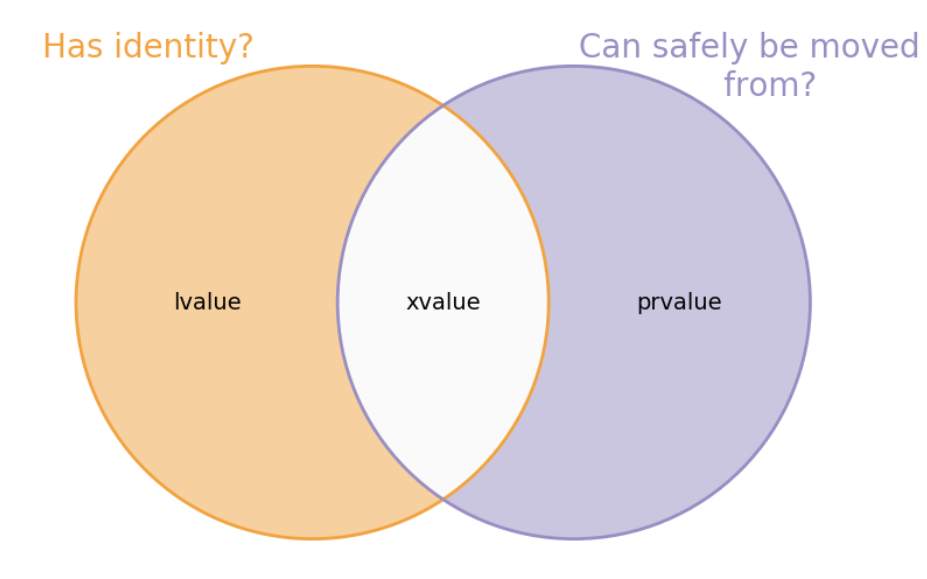
\includegraphics[width=0.3\linewidth]{pics/xvalue1.png}
		\caption{lvalue, rvalue and xvalue.}
		\label{fig:xvalue1}
	\end{figure}

	\item Distinguishing these three value categories is very important when you try to understand decltype deducting rule. I will introduce in "Generic programming" chapter.
	
	\begin{center}
		\begin{tabular}{|c|c|c|}
			\tophline
			& persist(Identity) & move \\
			\tophline
			lvalue & Yes & No \\
			\tophline
			pvalue & No & Yes \\
			\tophline
			xvalue & Yes & Yes \bottomhline
		\end{tabular}
	\end{center}

	\item In a simple word, xvalue is just value with identity and can be movable. In real life, it's  return value of std::move() or static\_cast<A\&\&>. A better introduction can be seen: " C++11 Tutorial: Explaining the Ever-Elusive Lvalues and Rvalues"

    \item Some examples of xvalue.
\begin{lstlisting}
string&& xvalue_fun();

xvalue_fun(); //After you call this fun, value still exist. 
xvalue_fun() = "hello"// You can modify because it persist.
&xvalue_fun(); //You can get address because it has identity.
string a = xvalue_fun();// call move constructor, can move.

struct A {
	int m;
};

A&& operator+(A, A); // a+a is xvalue
A&& f();  //f() is xvalue
f().m // f().m is also xvluae
A a;
A&& ar = static_cast<A&&>(a); static_cast<A&&>(a) is xvalue, but ar is lvalue	
\end{lstlisting}

\item After C++11, we added two new xvalues.
\begin{enumerate}
	\item \texttt{a[n]}, the built-in subscript expression, where one operand is an array rvalue;
	\item \texttt{a.m}, the member of object expression, where a is an rvalue and m is a non-static data member of non-reference
\end{enumerate}

	
    \item  \texttt{std::move} not only doesn't actually move anything, it doesn't even guarantee that the object it's casting will be eligible to be moved. The only thing you know for sure about the result of applying \texttt{std::move} to an object is that it return a xvalue. In fact, it's just type casting funciton. 

\begin{lstlisting}[frame=single, language=c++]
explicit Annotation(const std::string text)
: value(std::move(text))  //call copy constructor, not move constructor.
\end{lstlisting}
\begin{description}
	\item[Line 1:] That is constructor, we want to "move" text into value; this code doesn't do what it seems to, because text is const
\end{description}
	
	\item In summary: We want to move a lvalue, such as in swap function, so we have \texttt{std::move()} function. \texttt{std::move()} return neither lvalue nor prvalue, so we have to define a new type of value--xvalue.
	
\begin{center}	
		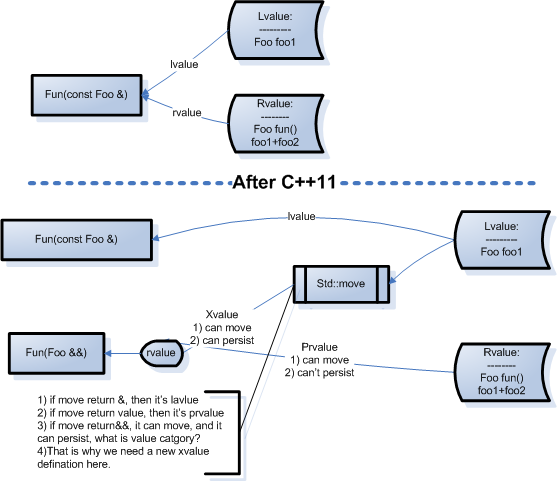
\includegraphics[width=0.7\linewidth]{pics/xvalue.png}
		\label{fig:xvalue}
    \end{center}
		
\end{itemize}

\subsection{Difference between xvalue and rvalue reference}
\begin{itemize}

	\item xvalue is defined based on rvalue reference. But you can't think that a rvalue reference is a xvalue. A named rvalue reference is lvalue, and unnamed rvalue reference is xvalue;
	
\begin{lstlisting}[frame=single, language=c++,mathescape=true]
void foo(int&& t) {
	//t is initialized with an rvalue expression, 
	//but is actually an lvalue expression itself inside function foo
}
	
std::string a;   //a, b, c are all lvalue.
std::string& b;
std::string&& c;
\end{lstlisting}

	\item The most important thing to remember is that value categories are a taxonomy of expressions. They are not categories of objects or variables or types. Getting this wrong is an immediate source of problems. Things that are declared as rvalue reference can be lvalues or rvalues. The distinguishing criterion is: if it has a name, then it is an lvalue. Otherwise, it is an rvalue. Understand this word is very important, In the previous code, r has name, so it is lvalue, When we use \texttt{std::move}, it "erase" the name by a function call, so unname rvalue reference is rvalue.
	
\begin{lstlisting}[frame=single, language=c++, mathescape=true]
void foo(int& );  // #1
void foo(int&& ); // #2

int&& r = 42;
foo(r); // will call #1, because r is lvalue, although type is rvalue reference.
foo(std::move(r)) //will call #2	
\end{lstlisting}	
	
	\item Why is there such confusion? Here are the circumstances under which it is safe to move something:\\
	1) When it's a temporary or sub-object thereof. (prvalue) \\
	2) When the user has explicitly said to move it.
\begin{lstlisting}[frame=single, language=c++]
SomeType &&Func() { ... }
	
SomeType &&val = Func();
SomeType otherVal{val}; // Do you really want to move 
	....
cout<<val; 
\end{lstlisting}
\begin{description}
	\item[Line 6:] what happen if you have forget you have "move"? it will crash! So standard said that \texttt{val} is lvalue. because it's a named rvalue reference.
\end{description}
	
    \item Another deep trap occurs when you implement the move constructor in a derived class. To address this issue, C++ introduced \texttt{std::move} to convert named rvalue references (lvalues) to unnamed rvalue references (xvalues). This helps to resolve the problem. "Effective Modern C++" item 25, "Use \texttt{std::move} on rvalue references, std::forward on universal references," expresses this idea more clearly.
\begin{lstlisting}[numbers=none]
Derived(Derived&& rhs):Base(rhs)//wrong: rhs is an lvalue
{
	// Derived-specific stuff
}
	
Derived(Derived&& rhs) : Base(std::move(rhs)){
	// good, calls Base(Base&& rhs)
}
\end{lstlisting}
	
\end{itemize}



\section{Universal(forwarding) reference }
\subsection{definition}

\begin{itemize}
	\item In pre-11 C++, it was not allowed to take a reference to a reference: something like \texttt{A\&\&} would cause a compile error. C++11, by contrast, introduces the following reference collapsing rules1:
	
\begin{lstlisting}[numbers=none]
A& & becomes A&
A& && becomes A&
A&& & becomes A&
A&& && becomes A&&
\end{lstlisting}

	
	\item With the help of the previous reference collapsing rule, we can define the forwarding reference type deduction rules: for lvalues and rvalues, we use different rules to deduce the type. If you pass an lvalue, then \texttt{T} will deduce to \texttt{T\&}, while for rvalues, it will deduce to \texttt{T}.
	
	\item Based on previous rule, we can use forwarding reference to judge if a var is lvalue. In the case you pass a \texttt{std::string} lvalue, then T will deduce to \texttt{std::string\&} or \texttt{const std::string\&}, for rvalues it will deduce to \texttt{std::string}.
\begin{lstlisting}[frame=single, language=c++]
template <typename T>
constexpr bool is_lvalue(T&&) {
	return std::is_lvalue_reference<T>{};
}

std::string a("Hello");
is_lvalue(std::string()); // false
is_lvalue(a); // true  	
\end{lstlisting}	
	
	\item You also co determine programmatic if an expression is rvalue or lvalue.
\begin{lstlisting}[numbers=none]
if (std::is_lvalue_reference<decltype(var)>::value) {
	// var was initialised with an lvalue expression
} else if (std::is_rvalue_reference<decltype(var)>::value) {
	// var was initialised with an rvalue expression
}

string&& xvalue_fun();
std::is_rvalue_reference<decltype(xvalue_fun())>::value //return true	
\end{lstlisting}	


    \item \textbf{In new C++ standard, universal reference has been renamed as forwarding reference}. It's more descriptive name, It tell you universal reference should always been used as forwarding a parameter. Universal references arise in two contexts. The most common is function template parameters; The second context is \texttt{auto\&\&}.  
    
    
    \item How can we recognize if something is a forwarding reference? 1)must be constrained T\&\& form, 2) type deduction happen. If the form of the type declaration isn't precisely type\&\&, or if type deduction does not occur, type\&\& denotes an rvalue reference.
\begin{lstlisting}
auto&& var2 = var1; // universal reference

template<typename T>
void f(T&& param); // universal  reference

template<class T, class Allocator = allocator<T>>
class vector {
	template <class... Args>
	void emplace_back(Args&&... args); //args is forwarding reference. 
};

//------------below are not universal reference----
template<typename T>
void f(std::vector<T>&& param); // rvalue reference, because it isn't T&& form

template<typename T>
void f(const T&& param); // with const

template<class T, class Allocator = allocator<T>>
class vector { 
public:
	void push_back(T&& x); //no type deduction happen here.
};
\end{lstlisting}

	\item \texttt{auto\&\&} is also forwarding reference, although it isn't used very often. If you don't want to dig too deep, you can skip below. If you use \texttt{std::forward} on your \texttt{auto\&\&} reference to preserve the fact that it was originally either an lvalue or an rvalue, your code says: Now that I've got your object from either an lvalue or rvalue expression, I want to preserve whichever valueness it originally had so I can use it most efficiently.  For \texttt{auto\&\&}, basic idea just like universal reference, you need to use \texttt{decltype(var)} to get type information when you use forward function on the universal reference. Please pay attention here: \texttt{var} was initialized with either an lvalue or rvalue, but \texttt{var} itself is an lvalue because named rvalues are lvalues.
\begin{lstlisting}[frame=single, language=c++]
auto&& var = some_expression_that_may_be_rvalue_or_lvalue;
use_it_elsewhere(std::forward<decltype(var)>(var));
\end{lstlisting}

	\item When to use \texttt{auto\&\&}. I will accept any initializer regardless of whether it is an lvalue or rvalue expression and I will preserve its constness. A good example of \\ "some\_expression\_that\_may\_be\_rvalue\_or\_lvalue;" is illustrated below:
\begin{lstlisting}[frame=single, language=c++]
std::vector<int> global_vec{1, 2, 3, 4};	
template <typename T>
T get_vector(){
	return global_vec;
}

template <typename T>
void foo(){
	auto&& vec = get_vector<T>(); 
	auto i = std::begin(vec);
	(*i)++;
	std::cout << vec[0] << std::endl;
}

foo<std::vector<int>>();  //return rvalue in line 9
std::cout << global_vec[0]; //global_vec[0] no change.

foo<std::vector<int>&>(); //return lvalue in line 9
std::cout << global_vec[0]; //global_vec[0] has change. 
\end{lstlisting}

\begin{description}
	\item[Line 9:] only \texttt{auto\&\&} work here. \texttt{auto}, \texttt{auto\&} , \texttt{const auto\&}, \texttt{const auto\&\&} all failed. 
\end{description}

\end{itemize}

\subsection{pros and cons of forwarding reference}
\begin{itemize}

	\item If you have a template class or template fun, universal reference is your only choice. An example can be seen in the last chapter, "decltype deduction" section.

	\item For overload method, more source code to write and maintain (two functions instead of a single template). For overload method, it can be less efficient. For example, consider this use of setName: w.setName("Adela Novak"); With the version of setName taking a universal reference, the string literal "Adela Novak" would be passed to setName, where it would be conveyed to the assignment operator for the std::string inside w. w's name data member would thus be assigned directly from the string literal; no temporary std::string objects would arise. With the overloaded versions of setName, however, a temporary std::string object would be created for setName's parameter to bind to, and this temporary std::string would then be moved into w's data member.

\begin{lstlisting}[numbers=none]
class Widget {
public:
	template<typename T>
	void setName(T&& newName) // newName is universal reference
	{ name = std::forward<T>(newName); }
...
	string name;    
};
\end{lstlisting}

    \item Overload has the poor scalability of the design. Widget::setName takes only one parameter, so only two overloads are necessary, but for functions taking more parameters, each of which could be an lvalue or an rvalue, the number of overloads grows geometrically, such as \texttt{make\_shared} function. It can provide the unify interface, and it supports variadic number. That is why \texttt{make\_unique} and \texttt{make\_shared} and emplace-kind function are possible.

\begin{lstlisting}[numbers=none]
template<class T, class... Args> 
shared_ptr<T> make_shared(Args&&... args); 

template<class T, class... Args> 
unique_ptr<T> make_unique(Args&&... args); 
\end{lstlisting}

    \item You can use universal reference,  but inside, you have to use forward function, and implementation is a little difficult. As a template, implementation must typically be in a header file. There are argument types that can't be passed by universal reference (see Item 30), and if clients pass improper argument types, compiler error messages can be intimidating (see "effective modern C++ item 27").

    \item Overloading on universal references almost always leads to the universal reference overload being called more frequently than expected. Perfect-forwarding constructors are especially problematic, because they're typically better matches than copy constructors for non-const lvalues, and they can hijack derived class calls to base class copy and move constructors. detail can be seen in "effective modern c++ item 26"

\end{itemize}

\subsection{Usage of forwarding reference}
\begin{itemize}
\item When to use universal references? 
	\begin{enumerate}
		\item First and foremost, it is only used in a template function. Inside the function, if you only need to read or write a value, you should use a reference or a const reference directly to avoid copying.
		
		\item For universal reference, you must forward it to constructor, container, object or function. And these four things will take different action toward lvalue and rvlaue. Most of time, in your universal function, you have a container(string is container too), because move container is much cheaper than copy it. You have to use reference, means that need refer a existing one, you refer it because you want to copy it inside of your template function.
		
		\item I will accept any initializer regardless of whether it is an lvalue or rvalue expression and I will preserve its constness.  This is typically used for forwarding (usually with \texttt{T\&\&}). The reason this works is because a "universal reference", \texttt{auto\&\&} or \texttt{T\&\&}, will bind to anything.  

		\item You might say, well why not just use a const auto\& because that will also bind to anything? The problem with using a const reference is that it's const! You won't be able to later bind it to any non-const references or invoke any member functions that are not marked const.
\begin{lstlisting}[frame=single, language=c++]
auto&& vec=some_expression_that_may_be_rvalue_or_lvalue;
auto i = std::begin(vec);
(*i)++;

auto        // will copy the vector, but we wanted a reference
auto&       // will only bind to modifiable lvalues
const auto& // will bind to anything but make it const, giving us const\_iterator
const auto&& //will bind only to rvalues with const, It's not univerisal reference any more. 
\end{lstlisting} 
	\end{enumerate}

	\item Forwarding reference is used in three important STL functions \texttt{emplace\_back}, \texttt{make\_shared} and \texttt{make\_unique}. You can use them as a good example to study when and where you can use forwarding reference in your own project.
	\begin{enumerate}
		\item \textbf{variadic template}, because it need to receive \textbf{any number and any type} parameter.

		\item \textbf{Forwarding reference}, because it's template, and I also want to keep rvalue semantic to improve efficiency. These three functions has "COPY" semantic inside. The more you know these three functions, the better you understand forwarding reference.
	\end{enumerate}
\end{itemize}


\subsection{std::move and std::forward implementation}
\begin{itemize}
	\item Basic implementation of \texttt{std::move}.
\begin{lstlisting}[numbers=none]
template<typename T> // in namespace std
typename remove_reference<T>::type&&  move(T&& param){
	using ReturnType = typename remove_reference<T>::type&&; 
	return static_cast<ReturnType>(param);
}
\end{lstlisting}
	
	\item Basic implementation of \texttt{std::forward}.
\begin{lstlisting}numbers=none]
template<typename T>
T&& forward(typename remove_reference<T>::type& param){
	return static_cast<T&&>(param);
}
\end{lstlisting}

	\begin{figure}[h]
	\centering
	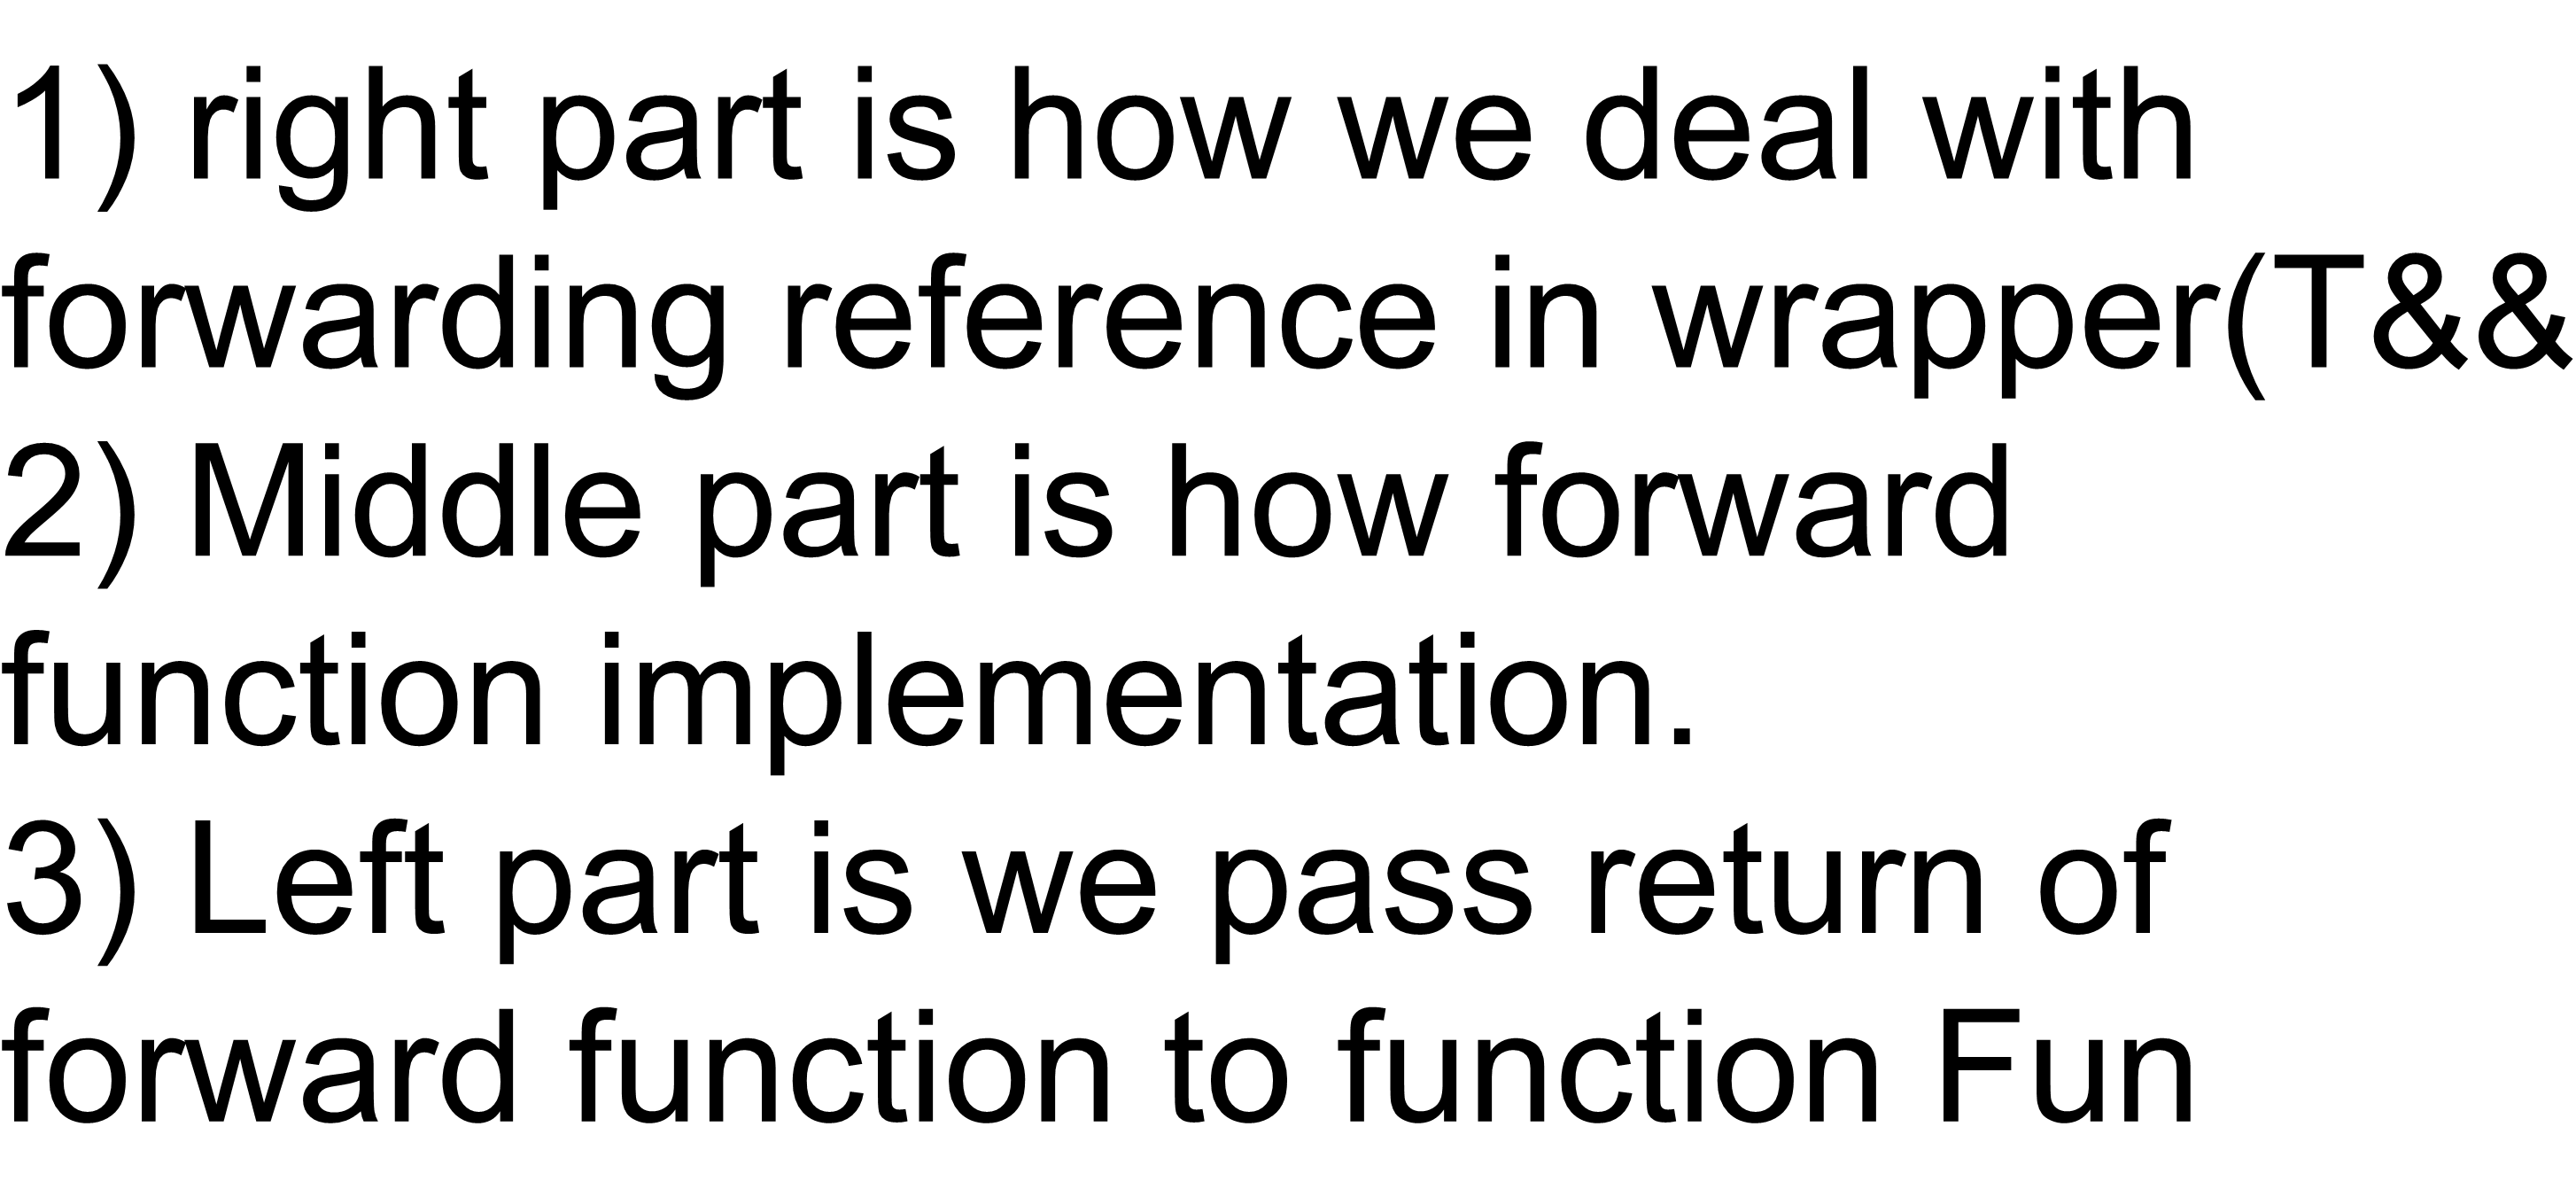
\includegraphics[width=0.85\linewidth]{pics/rvalue_ref.png}
	\caption{move and forward implementation}
	\label{fig:rvalueref}
\end{figure}

    \item A few more explanations about previous implementation:
    \begin{enumerate}
        \item In forward function, why parameter is \texttt{std::remove\_reference\_t<T>\& t}? Forward mainly used inside another funciton, outside function parameter has name, so the parameter is lvalue.
\begin{lstlisting}
forward(int& r1); #1
forward(int&& r1); #2
	
void fun(int&& r){
	int& r1 = r;  //OK, r is lvalue
	//int&& r1 = r;  //error: cannot bind 'int' lvalue to 'int&&'
	forward(r) //it will call #1, not #2, because r is lvalue.
}
int r = 2;
fun(std::move(r));
\end{lstlisting}

    \item Why \texttt{std::move} use forwarding reference as parameter. Just for more generic. We have introduced \texttt{vector<bool>} before, it returns a proxy value and it's rvalue. It's a extreme case, and I admit that. But in generic(template) programming, you will meet it too.
\begin{lstlisting}[]
std::vector<bool> v{true};
std::move(v[0]); // std::move on rvalue, OK
\end{lstlisting}
        \end{enumerate}
    
    \item The new standard has two overloaded \texttt{std::forward} template functions. The next part is a little theoretical. If you don't want to go that deep, you can skip it because you can still use \texttt{std::forward} properly even if you don't know the implementation details behind it.  
\begin{lstlisting}
template< class T >
constexpr T&& forward( std::remove_reference_t<T>& t ) noexcept;

template< class T >
constexpr T&& forward( std::remove_reference_t<T>&& t ) noexcept;	
\end{lstlisting}

	\item Why do we need the second overloaded function? It is for a very special case. The below code shows a scenario where we will use the second overload.
\begin{lstlisting}
template< class T >
constexpr T&& forward( typename std::remove_reference<T>::type& t ){
	std::cout << __PRETTY_FUNCTION__ << '\n';
	return static_cast<T&&>(t);
}
template< class T >
constexpr T&& forward( typename std::remove_reference<T>::type&& t ){
	std::cout << __PRETTY_FUNCTION__ << '\n';
	return static_cast<T&&>(t);
}

void g(int&)  { std::cout << __PRETTY_FUNCTION__ << '\n'; }
void g(int&&) { std::cout << __PRETTY_FUNCTION__ << '\n'; }

template<class T>
auto f(T&& t){
	std::cout << __PRETTY_FUNCTION__ << '\n';
	g(forward<decltype(forward<T>(t).get())>(forward<T>(t).get()));
}

struct foo{
	int i = 42;
	int  get() && { std::cout << __PRETTY_FUNCTION__ << '\n'; return i; }
	int& get() &  { std::cout << __PRETTY_FUNCTION__ << '\n'; return i; }
};

f(std::move(foo1)); // output of this statement is below
\end{lstlisting}

	\item Below is the output the \texttt{f(std::move(foo1));},  Let me explain it in detail about what happen behind the output. 
\begin{lstlisting}
auto f(T &&) [T = foo]   #1
T &&forward(typename std::remove_reference<T>::type &) [T = foo] #2
int foo::get() && #3
T &&forward(typename std::remove_reference<T>::type &&) [T = int] #4
void g(int &&) #5
\end{lstlisting}
   
    \begin{enumerate}
    	\item template \texttt{f} function has forwarding reference. When we input rvalue, template parameter will be deducted by \texttt{T}, not \texttt{T\&}, \#1 shows the function type.
    	
    	\item Inside \texttt{f}, t is \texttt{foo\&\&}, but t itself is lvalue. The third forward function in line 18 returns T\&\&(foo\&\&), that is to say \texttt{forward<T>(t)} return a rvalue. \#2 shows the third forward function type. 
    	
    	\item Once we have \texttt{foo\&\&}, we use it call \texttt{foo::get()}, it will call rvalue reference version. \#3 demonstrate it. 
    	
    	\item In line 18, from \#3 we know that get return int, so 1) The first forward will be deducted by int. 2) get which return int is rvalue, so we need forward function can recieve the rvalue, so the first forward function is dedecuted by \texttt{std::remove\_reference<T>::type \&\&}, \#4 proves this.
    	
    	\item The first forward return int \&\&, so it call g(int \&\&) just like \#5 shows . 
    	
    	\item \texttt{PRETTY\_FUNCTION} is a powerful tool when you analyze the instantiation of a template function.
    \end{enumerate}
    
    
    \item There are two important points to help you understand \texttt{std::move} and \texttt{std::forward}. One is forwarding reference deduct rule, the other is reference collapse rules.
\end{itemize}


\section{Function interface-parameter}

\subsection{read-copy function parameter design}

\begin{itemize}

	\item By now, you may imagine that you have a function with parameters, and then you have three main operations inside to operate on the parameters: 1) only read, 2) copy from the parameters, and 3) write to parameters. For a context where only reading is required, "\texttt{const type\&}" is the best option. For writing, "\texttt{type\&}" is good because you don't need to write any new thing into the prvalue. Based on the previous explanation, the code below will not compile.
\begin{lstlisting}[numbers=none]
writeFun(Foo &);
writeFun(foo1+foo2) //ERROR
\end{lstlisting}

	\item In a 'read-copy' scenario, things become interesting. You have an original object, but in your function, you want to copy from it, perhaps modify it, or return this copied version. In any case, a kind of 'copy' operation does happen inside the function.

    \item For only read build-in type, such as \texttt{int, char, short, double}. You can use value directly, it has the same performance as reference. If you want to change it, you still need to use reference. If the function \textbf{read} in some object and \textbf{copy} it inside the function. You need to consider the parameter design. When I say \textbf{copy}, it could be: 1) call constructor inside fun 2) assign these values to other.3) put values into container. For examples \texttt{make\_unique,} \texttt{emplace\_back} are this kind of functions.

	\item The move constructor and move assignment operator give us an idea how to improve the function interface design.  For rvalue, we can move directly. Our goal is that we can use move for rvalue, so there are four options: 

	\begin{enumerate}
		\item Overload fun to support \texttt{const Foo\&} and \texttt{Foo \&\&}. Copy constructor is typical example of this strategy. So usually function which accepts rvalue reference doesn't exist by itself, it just stay with another version to accept lvalue, \texttt{fun(const Foo\& foo);}
\begin{lstlisting}[frame=single, language=c++]
fun(const Foo& foo); //lvalue reference
fun(Foo&& foo); //rvalue reference
fun(foo1+foo2)  // call move constructor.
fun(f_return_foo()); // call move constructor.
\end{lstlisting}		
		
		\item Use pass-value \texttt{fun(Foo)}. We will introduce it later.
		\item Use pass-rvalue-reference \texttt{fun(Foo\&\&)}.
		\item Use forwarding reference \texttt{fun(T\&\&)}.
	\end{enumerate}
	
\begin{center}


\begin{tabular}{|p{0.25\textwidth}|p{0.32\textwidth}|p{0.32\textwidth}|}
\tophline
 & \textbf{lvalue}  & \textbf{rvalue} \\
\tophline
copyFun(Foo foo) & \specialcell[t]{copy parameter,move inside} & \specialcell[t]{move parameter, move inside} \\
\tophline
copyFun(Foo \&)  & copy inside & (NOT support) \\
\tophline
copyFun(const Foo \&) & copy inside & copy inside \\
\tophline
copyFun(Foo \&\&)  & (NOT support) & move inside \\
\tophline
\specialcell[t]{template<T\&\&> \\
copyFun(T \&\&)}  & copy inside & move inside 
\bottomhline
\end{tabular}

\end{center}

\subsubsection{Only value solution}

	\item In the book 'Effective Modern C++', Item 41 expresses the idea very clearly that copyable parameters that are cheap to move should be passed by value, and it also provides some good examples. A value parameter example can be see in the below code:

\begin{lstlisting}[frame=single, language=c++]
std::vector<std::string> sorted(std::vector<std::string> names){
	std::sort(names);
	return names;
}

std::vector<std::string> sorted_names1 = sorted( input_names ); //copy here
std::vector<std::string> sorted_names2 = sorted( get_names() ); //copy elision
\end{lstlisting}
\begin{description}
	\item[Line 7:] \texttt{get\_names()} is an rvalue expression; move or omit the copy with copy elision optimization.
\end{description}

%    \item If we use reference parameter instead value parameter, we have to copy it inside of function. We can't change because it's const reference, so have to copy it inside first. 
%
%\begin{lstlisting}[numbers=none]
%std::vector<std::string> sorted2(std::vector<std::string> const& names) {
%	std::vector<std::string> r(names);   // copy happen here
%	std::sort(r);  //change
%	return r;    //return
%}
%\end{lstlisting}
%
%
%
%\item A basic explanation is below:
%\begin{center}
%	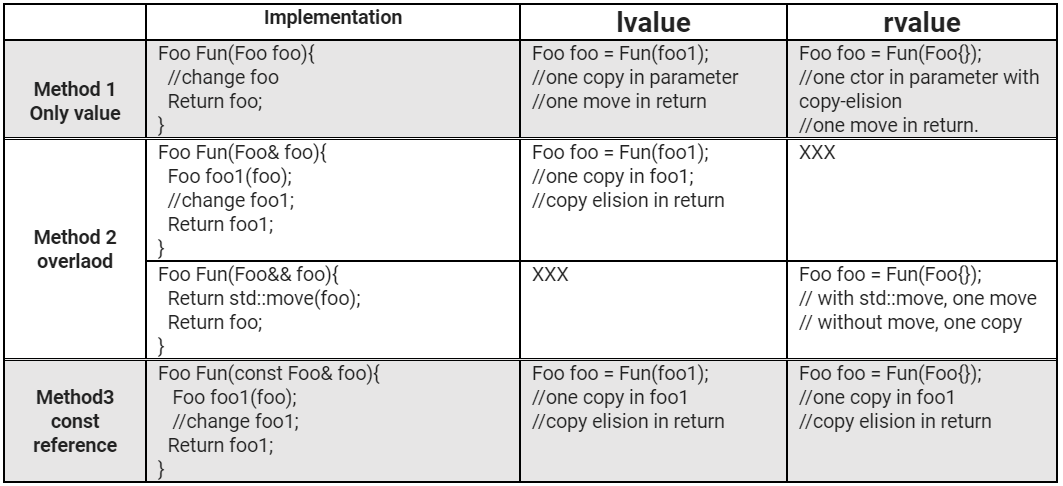
\includegraphics[scale=0.5]{pics/copy1.png}
%\end{center}
%
%\item For left value, method 1 has extra move operation.
%
%\begin{center}
%\begin{tabular}{|c|c|c|c|}
%	\hline
%	left value input	& constructor & copy & move  \\
%	\hline
%	Method 1 & 1 & 1 & \textbf{\underline{1}} \\
%	\hline
%	Method 2&  1& 1 & 0  \\
%	\hline
%	Method 3&  1&  1& 0 \\
%	\hline
%\end{tabular}
%\end{center}
%
%\item For right value, method 1 has extra move operation, but method 3 has extra copy
%
%\begin{center}
%\begin{tabular}{|c|c|c|c|}
%	\hline
%	right value input	& constructor & copy & move  \\
%	\hline
%	Method 1 & 1 & 0 & 2(1)  \\
%	\hline
%	Method 2 & 1 & 0 & 1 \\
%	\hline
%	Method 3 & 1 & \textbf{\underline{1}} & 0 \\
%	\hline
%\end{tabular}
%\end{center}

%\item Comparison of three methods. 
%\begin{enumerate}
%	\item For method 1 for rvalue,  if you use -fno-elide-constructors, then it use 2 move, otherwise use 1 move(Copy-elision happens when we pass the parameter into the function). Even we use 2 move, \textbf{compared with method 3, it doesn't need a copy.}
%	
%	\item Method 2 is the best, but you need to write two overload functions.
%	
%	\item For method 3, When return, you can have RVO, no copy or move when we return. Only one copy inside the function.
%	
%	\item If don’t use method 2.  We are taught that reference is more efficient than value(it can avoid coping). But in our specific scenario(we still copy inside the function even we use reference). \texttt{if move is cheaper than copy, then method1 is better than method 3}. Although for lvalue, It use one more move, but for rvalue, it also use move, not copy(expensive operation).
%	  
%\end{enumerate}
%
%
%\item summary:
%\begin{enumerate}
%	
%	\item For non-cheap-move, such as all primitive type included class, move is just like copy, \textbf{So reference WIN!}
%	
%	\item For c++11 and cheap-move semantic, \textbf{value WIN!} The same idea can be seen in the "more effective C++ item 41". Don’t copy your function arguments. Instead, pass them by value and let the compiler do the copying. 
%	
%	\item For = operator in resource wrapper class, we don't need return value, but return reference, In this way, \textbf{value WIN!}. Detail can be found in use swap to implement = operator below. \textbf{That is the famous principal four and half rule.} One copy constructor, one move ctor, one value assignment, , one destructor, one swap(half).
%	
%\end{enumerate}
%

	\item You can apply this guideline immediately in assignment operators. The canonical, easy-to-write, always-correct, strong-guarantee, copy-and-swap assignment operator is often seen written this way. That is the famous principal \textbf{four and half rule.} One copy constructor, one move ctor, one value assignment, , one destructor, one swap(half).
\begin{lstlisting}[frame=single, language=c++]
T& T::operator=(T const& x){ 
	T tmp(x);          
	swap(*this, tmp);  
	return *this;      
}

T& operator=(T x){ 
	swap(*this, x);
	return *this;   
}
\end{lstlisting}
\begin{description}
	\item[Line 2 to 4:] \texttt{x} is a reference to the source. copy construction of tmp does the hard work. trade our resources for tmp's. our (old) resources get destroyed with tmp 
	
	\item[Line 7 to 10:] A better one is below. \texttt{x} is a copy of the source; hard work already done. trade our resources for x's. our (old) resources get destroyed with \texttt{x}.
\end{description}

	\item You can't apply this idea into the copy constructor, otherwise it will cause dead recursive.
\begin{lstlisting}[frame=single, language=c++]
Class A{
	A(A a){..} //Can't declare in this way.
}
\end{lstlisting}

	\item Two good articles about this topic are:"Want Speed? Pass by Value." and "WANT SPEED? DON'T (ALWAYS) PASS BY VALUE."

\subsubsection{Use rvalue  reference or forwarding reference}

    \item A more academic options is to just pass rvalue reference to deal with lvalue and rvalue at the same time. This idea can be googled by "Pass By Rvalue Reference Or Pass By Value"; But for lvalue, you need a help function here.
\begin{lstlisting}[frame=single, language=c++]
template<typename T>
T copy_to_temp(const T& t) { return t; }

SomeType t; 
s.initByRef(copy_to_temp(t)); //t is lvalue, need copy first.
\end{lstlisting}

    \item The same idea can be applied to move-only types (such as \texttt{unique\_ptr<T>})
\begin{lstlisting}[frame=single, language=c++]
template<typename T>
T move_to_temp(T& t) { return std::move(t); }

void foo(unique_ptr<SomeType>&& param);
unique_ptr<SomeType> p;
foo(move_to_temp(p)); //note: this does move, p will become empty 
foo(std::move(p)); //here, p will not become empty.  
\end{lstlisting}


    \item Frankly speaking, it's not mainstream idea, because it's a little difficult to understand and need extra help funciton. keep just for a option.

%VMore interesting example:
%\begin{lstlisting}[frame=single, language=c++]
%template<typename T>
%T move_to_temp1(T& t) { return std::move(t); }
%T&& move_to_temp2(T& t) { return std::move(t);}


%void foo(unique_ptr<SomeType>&& param);

%unique_ptr<SomeType> p;
%foo(move_to_temp1(p));  //compile ok, return value is prvalue
%foo(move_to_temp2(p));  //compile ok, return value is xvalue
%\end{lstlisting}
%\begin{description}
	%\item[Line 2:] here move constructor is called when return to a value
	%\item[Line 4:] here no move constructor is called, just reference value assignment.
%\end{description}



    \item The last option is universal reference. At this time, you have to use \texttt{std::forward} 
\begin{lstlisting}[numbers=none]
template<typename T>
Fraction reduceAndCopy(T&& frac){ //only used in template function 
	frac.reduce();
	return std::forward<T>(frac); // have to use std::forward<T>
} 
\end{lstlisting}

	\item Below is a very important summary. Please read it carefully and make sure you understand it.
	\begin{enumerate}
		\item Overloading with const lvalue reference and rvalue reference is the most common strategy to deal with read-copy kind of function interface design. It has the highest efficiency, but you need to write two functions. 
\begin{lstlisting}[numbers=none]
void addName(const std::string& newName){
	names.push_back(newName); 
} 

void addName(std::string&& newName) {
	names.push_back(std::move(newName)); 
} 
\end{lstlisting}
		\item Only a value parameter is also an option when you 1) make sure the copy happens inside the function and 2) the move is cheap. The advantage is that you only need to write one function, but you have one more move operation for both lvalue and rvalue. At the same time, it has more restrictions on the application context.
\begin{lstlisting}[numbers=none]
void addName(std::string newName) { 	
	names.push_back(std::move(newName)); 
} 
\end{lstlisting}		
		\item For forwarding reference, you only need to maintain one function and the efficiency is just like an overloaded function. However, it has its own problems. The details can be seen in the section titled "Pros and Cons of Forwarding Reference". 
\begin{lstlisting}[numbers=none]
template<typename T> 
void addName(T&& newName) { 
 	names.push_back(std::forward<T>(newName)); 
} 
\end{lstlisting}
	\end{enumerate}

\end{itemize}

\section{funciton interface-return}
%\subsection{funtion return basic introduction}
%\begin{itemize}
%	\item \textbf{These are two most important knowledge to understand function return.}
%	\begin{enumerate}
%		\item For no RVO, there are two steps when we return value.
%		\item RVO is a kind of copy elision. In RVO implementation, we implicit pass the result by reference.
%\begin{lstlisting}
%X bar(){
%	X xx;
%	return xx;
%}
%	
%X result = bar(); //change bar definition to below:
%void bar(x &__result){
%	__result.X::X() // default constructor call
%	....
%	return
%}
%\end{lstlisting}
%
%	\end{enumerate}
%	
%	\item Three basic knowledges about function return when no RVO:
%	\begin{enumerate}
%		\item It's very important understand there are two phrases when you return from function. The first step  is from inside fun fauto to outside of function ftemp(unname tempory), then fauto disappear(call destructor for value).  Then in second step, \textbf{Move} from ftemp to flast. because ftemp is rvalue.
%\begin{lstlisting}[numbers=none]
%Foo fun(){
%	return fauto;
%}
%		
%Foo flast = (ftemp created here)fun();
%\end{lstlisting}
%		\item ftemp is not on the stack, so you can use const ref or rref to prolong its life. ftemp is same with fauto, but maybe not same with flast(Will happen implicit conversion sometimes)
%\begin{lstlisting}[frame=single, language=c++]
%Foo fun(){
%	return fauto;
%}
%		
%const Foo& flast = (ftemp created here)fun();
%Foo&& flast = fun();
%\end{lstlisting}
%
%	\end{enumerate}
%	
%	\end{itemize}

\subsection{return plain reference} 
\begin{itemize}
	
	\item Don't return a reference or pointer to private member variables through your public member functions. It will break encapsulation. At the same time, \textbf{never} return a reference that refers to a local variable; it will cause a dangling reference problem. When the client programmer uses a reference beyond its lifetime, the bug will typically be intermittent and very difficult to diagnose. Indeed, one of the most common mistakes that programmers make with the standard library is to use iterators after they are no longer valid, which is pretty much the same thing as using a reference beyond its lifetime.
	
\begin{lstlisting}[frame=single, language=c++, mathescape=true]
string& a = FindAddr( emps, "John Doe" );
emps.clear(); //invalid a here
cout << a; //a has been dangling  
\end{lstlisting}
	
	\item Why \textbf{don't} we return plain reference?
	\begin{enumerate}
		\item You want to return a reference to avoid copy of stack obj inside of function, but in fact it's totally wrong. We have RVO and implicit \texttt{std::move}.
	
		\item If you want to return a non-stack object, you can create an object with new and then return a pointer to it directly. Alternatively, you can use a reference parameter for read-only access by passing in a const reference. In this case, you don't need to return anything at all. Finally, you can use a reference parameter for write access, in which case you also don't need to return anything; the modification will be applied directly to the inputted reference. So when do we use plain reference return?
	\end{enumerate}
	
	
	\item As far as I know, return plain reference only happens: You input a reference first, such as overload \verb=<<=. Member function return some member data, such as  assignment operator and overload \verb=[]= inside a class. \texttt{=} and \texttt{<<} are for support cascading syntactic usage: such as \texttt{cout<<a<<b}, \texttt{a=b=c}.  \texttt{[]} is for support assignment \texttt{obj[3]= 12}.  That is all.

\begin{lstlisting}[numbers=none]
operator =  //three operators have "a pair of bars" :)
operator []
operator << and >>
\end{lstlisting}
	
	\item If you want to return reference,  there is a defensible option that allows returning a reference and thus avoiding a temporary. But it's your last resort.
\begin{lstlisting}[numbers=none]
const string& FindAddr( /* pass emps and name by reference */ ){
	for( /* ... */ ){
		if( i->name == name ){
			return i->addr;
		}
	}
	static const string empty; 
	return empty;
}
\end{lstlisting}

	\item Rvalue reference is also a reference, so if we have a reason not to return a reference from a function, all of these reasons are also valid for rvalue reference. The most common case for returning an rvalue reference is \texttt{std::move}. It doesn't involve any move action inside the function but is just a type-casting operation.
	
%	\item If you want to return plain reference, or rvalue reference from a function, you have to input a plain reference or rvalue reference first, because you can't return any reference bound to local stack obj.
%	
%\begin{lstlisting}
%A&& rrfun1(A&& arg){
%	return std::move(arg);//arg is lvalue, so use move	
%}
%	
%A&& rrfun2(A& arg){
%	return std::move(arg);
%}
%	
%A a;
%A b= rrfun1(std::move(a) );
%A b = rrfun2(a); // a has been moved to b. 
%A&& c = rrfun2(a);
%\end{lstlisting}
%\begin{description}
%	\item[Line 12:] will not call move constructor at all. So you mean that I want to keep watch for a while, and obj a is still intact right now.
%\end{description}
 
	
	\item Next we talk rvalue reference qualifier. Please see two examples below. More details can be googled  "C++ Gems: ref-qualifiers"
	\begin{enumerate}

	\item The ref-qualifier \texttt{\&\&} says that the second function is invoked on rvalue temporaries, making the following move, instead of copy.
\begin{lstlisting}
struct Beta {
	Beta_ab ab;
	Beta_ab const& getAB() const& { return ab; }
	Beta_ab getAB() && { return move(ab); }// correct, 
};

Beta_ab ab = Beta().getAB(); //call line 4 function, not line 3 funciton.
\end{lstlisting}
	
	\item What should we return from ref-qualifier member function? value or rvalue reference?  In fact, return value is better if you just want to copy from the return value from the member function. If you return the rvalue reference, maybe it has dangling reference problem.  
\begin{lstlisting}
class Widget { 
	DataType values; 
public: 
	DataType& data() & { return values; } 
	DataType data() && { return std::move(values); }
	DataType&& data_ref() && { return std::move(values); }
};

auto d1 = Widget().data(); 
auto d2 = Widget().data_ref(); 
auto&& d3 = Widget().data_ref();
\end{lstlisting}
\begin{description}
	\item[Line 9:] Note that auto is deduced to be Widget type okay, rvalue returned by function call moves construct d1 if compiler implemented RVO copy elision, the move in move construct likely be elided.
	
	\item[Line 10:] okay, rvalue reference returned by function call moves construct d2.
	
	\item[Line 11:]	\texttt{auto\&\&} is a universal reference, deduced to be DataType\&\& rvalue reference. dangling reference, bad. temporary copy of \texttt{Widget} is destroyed, so d3 is a dangling rvalue reference to values in the destroyed copy.  Pay attention here, d3 will not prolong the temporary Widget() life, because it is just DataType(Widget's member) reference type. That is why we have dangling reference problem. 	
\end{description}
	
	\end{enumerate}

	\item A few good articles you can dig deeper:
	\begin{enumerate}
		\item Efficiency of C++11 push\_back() with std::move versus emplace\_back() for already constructed objects.
		\item view the default functions generated by a compiler?
		\item One variable initialization form to rule them all, via mandatory elision.
		\item Episode Eleven: To Kill a Move Constructor
	\end{enumerate}

	\item A return value is better than returning an rvalue reference. It has clearer semantics and supports RVO.

\end{itemize}

\subsection{return value-RVO}

\subsubsection{common RVO cases}
\begin{itemize}
	\item RVO is a kind of copy elision. In RVO implementation, we implicitly pass the result by reference into the function. \textbf{It happens when you return a value from a function.} The type of the \textbf{local} object is the same as that returned by the function. The local object is what's being returned.
\begin{lstlisting}
X bar(){
	X xx;
	return xx;
}

X result = bar(); //change bar definition to below:
void bar(x &__result){ pass the result by reference here. 
	__result.X::X() // default constructor call
	....
	return
}	
\end{lstlisting}

	\item parameter is not eligible for RVO. 
		\begin{enumerate}
			\item value parameter will use move in the implicitly, you don't need explicit call \texttt{std::move}.
			\item lvalue reference parameter usually should not be move, just copy.
			\item for rvalue reference, you can use \texttt{std::move} to move the resource to the return value.
		\end{enumerate}
	
	\item Some common cases of copy-elision:
	\begin{enumerate}
		\item RVO and name RVO. For name RVO, \texttt{t} has a name. It's called NRVO. 
\begin{lstlisting}[numbers=none]
Thing f() {
	Thing t;
	return t; //Name RVO
}

Thing f() {
	return Thing(); //RVO, no name, just temporary
}
\end{lstlisting}

	\item temporary is passed by value.
\begin{lstlisting}[numbers=none]
void foo(Thing t);
foo(Thing());
\end{lstlisting}

	\item exception is thrown and caught by value.
\begin{lstlisting}[numbers=none]
void foo() {
	Thing c;
	throw c;
}

try {
	foo();
}
catch(Thing c) {  
}
\end{lstlisting}

	\end{enumerate}

\end{itemize}

\subsubsection{RVO limitations}
\begin{itemize}
	\item Different named object samples will not trigger RVO.
\begin{lstlisting}[numbers=none]
RVO MyMethod (int i){
	RVO rvo;
	rvo.mem_var = i;
	if (rvo.mem_var == 10)
		return RVO();
	return rvo; 
}
\end{lstlisting}
	
	\item returning a parameter or Global.
\begin{lstlisting}[numbers=none]
Snitch global_snitch;
Snitch ReturnParameter(Snitch snitch) {
	return snitch; //no RVO here, it's parameter
}
Snitch ReturnGlobal() {
	return global_snitch; //no RVO here either, it's global
}
\end{lstlisting}

	\item Return by \texttt{std::move()}. That is the most obvious error for some basic C++ developers, who do not understand RVO very well.
\begin{lstlisting}[numbers=none]
Snitch CreateSnitch() {
	Snitch snitch; //Basicly, RVO will trigger here
	return std::move(snitch); //but when you use move, it disable RVO
}
\end{lstlisting}
	
	\item When return member, even an unnamed variable, RVO will not trigger. 
\begin{lstlisting}[numbers=none]
struct Wrapper {
	Snitch snitch;
};

Snitch foo() {
	return Wrapper().snitch; 
}

Snitch s = foo(); //no RVO here. call snitch constructor and move
\end{lstlisting}

	\item A common error is when there is no RVO, use \texttt{std::move} to avoid copy: but Although parameter is not eligible for RVO, or different path is not eligible, but you don't need to explicit use \texttt{std::move}, the compiler will use them implicitly.

\begin{lstlisting}
Widget makeW(Widget w){
	.....
	return w  //w is parameter, compiler will call move 
	//return std::move(w), don't do it. compiler call move. 
} 	
\end{lstlisting}

	\item If a function return value, and you want to return \textbf{a rvalue reference parameter}, you have to use \texttt{std::move} in the return.
\begin{lstlisting}[frame=single, language=c++]
Matrix operator+(Matrix&& lhs, const Matrix& rhs){
	lhs += rhs; 
	return std::move(lhs); //move into return value, high efficiency. 
	//return lhs  //will copy, so low efficiency
} 	
\end{lstlisting}	
\begin{enumerate}
	\item lhs is not local object, but parameter, so No RVO. 
	
	\item you may say: but lhs is rvalue reference, but lhs is name rvalue reference. It's lvalue.
	
	\item Just like you pass a lvalue reference, you can't move it unless you want to do it explicitly. That is why we need \texttt{std::move} here. Frankly speak, this is typical example to demonstrate when you can use \texttt{std::move} when you return value, so I recommend you to remember it.
\end{enumerate}

\end{itemize}

\subsubsection{Some practical demos and analysis}
\begin{itemize}
	
	\item Given below code as experiment code:
\begin{lstlisting}[frame=single, language=c++]
class Snitch {   // Note: All methods have side effects
	Snitch() { cout << "c'tor" << endl; }
	~Snitch() { cout << "d'tor" << endl; }
	
	Snitch(const Snitch&) { cout << "copy c'tor" << endl; }
	Snitch(Snitch&&) { cout << "move c'tor" << endl; }
	
	Snitch& operator=(const Snitch&) {
		cout << "copy assignment" << endl;
		return *this;
	}
	
	Snitch& operator=(Snitch&&) {
		cout << "move assignment" << endl;
		return *this;
	}
};
	
Snitch CreateSnitch() {
	return Snitch();
}
	\end{lstlisting}
	
	\item test 1 and output. 
\begin{lstlisting}[frame=single, language=c++]
int main() {
	Snitch s = CreateSnitch();
}
\end{lstlisting}
\begin{description}
	\item[Output:] The compiler switch and its output:
	\begin{verbatim}
		with -fno-elide-constructors
		c'tor    //Snitch()
		move c'tor  //Snitch() to return value
		d'tor       //Snitch() destroy
		move c'tor //return value to s
		d'tor     //return value destroy
		d'tor     //s destroy
	------------------------------
		without -fno-elide-constructors
		c'tor   //s
		d'tor   //s destroy
	\end{verbatim}
\end{description}
	
	\item test 2 and output
	\begin{lstlisting}[frame=single, language=c++]
int main() {
	Snitch s;
	s = CreateSnitch();
}
	\end{lstlisting}
\begin{description}
	\item[Output:] The compiler switch and its output:
	\begin{verbatim}
		with -fno-elide-constructors
		c'tor    //Snitch s
		c'tor    //Snitch() in side CreateSnitch
		move c'tor  //Snitch() to return value
		d'tor       //Snitch() destroy
		move assignment //return value to s
		d'tor     //return value destroy
		d'tor     //s destroy
	----------------------	
		without -fno-elide-constructors
		c'tor   //Snitch s
		c'tor   //Snitch()
		move assignment //s has been implicit passed to CreateSnitch, 
		//so s = Snitch() happen inside CreateSnitch
		d'tor   //Snitch() destroy
		d'tor   //s destroy
	\end{verbatim}
\end{description}

	\item test 3 and output.
\begin{lstlisting}[frame=single, language=c++]
Snitch CreateSnitch() {
	return Snitch();
}
	
Snitch CSnitch(Snitch&& rs) {
	return rs;
}
	
int main() {
	Snitch s = CSnitch(CreateSnitch());
}
\end{lstlisting}
\begin{description}
	\item[Output:] The compiler switch and its output:
	\begin{verbatim}
		with -fno-elide-constructors
		c'tor    //
		copy c'tor    //
		d'tor       /
		copy c'tor    //
		copy c'tor    //
		d'tor       /
		d'tor     //r
		d'tor     //
	-------------------------
		without -fno-elide-constructors
		c'tor   //Snitch s
		copy c'tor //
		d'tor   //Snitch() destroy
		d'tor   //s destroy
	\end{verbatim}
\end{description}
\end{itemize}


%\subsubsection{return mulit value}
%\begin{itemize}
	%\item You can return pair, tuple and variant. 
	%\item for example, map.insert just return a pair. 
	%\item how to use variant as return value? find a example here
%\end{itemize}

\subsection{Function interface design summary}

\begin{itemize}
			\item Based on the previous concepts of rvalue reference, forwarding reference, and RVO, the following figure illustrates the principles of function interface design for parameters and return values.
		\begin{center}
			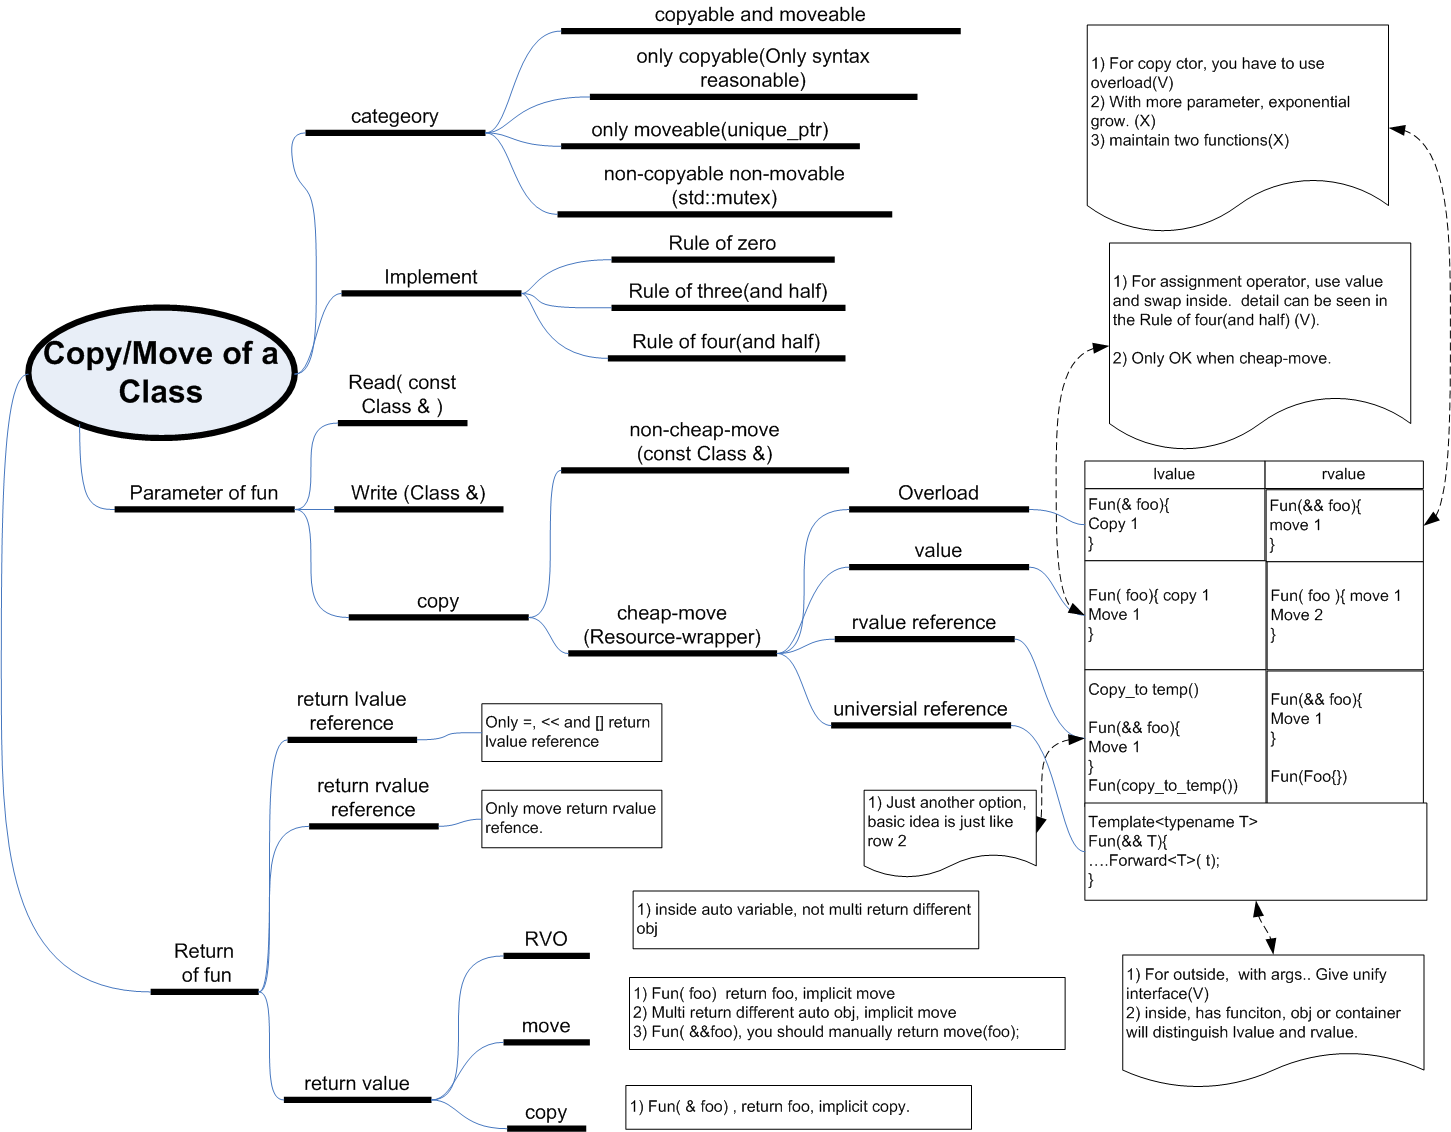
\includegraphics[width=1.0\linewidth]{pics/move.png}
		\end{center}
	
		\item We usually don't return references, whether they are lvalue references or rvalue references. Only three operator overloads return lvalue references. \texttt{std::move} returns an rvalue reference. It doesn't involve value semantics, just a type change. All the others return values. That's all!
	
		\item If a function returns a value and it's only a copyable lvalue, you should return the value directly. For rvalue reference parameters, you should use \texttt{std::move} explicitly. Because an rvalue reference is still a reference, not a local auto object, if we don't use \texttt{std::move}, it will be copied when we return it. Use \texttt{std::forward} on universal references the last time they are used.
	
\begin{lstlisting}[numbers=none]
Matrix operator+(Matrix& lhs, const Matrix& rhs) {
	return lhs //for lvalue refence, return it .
}
	
Matrix operator+(Matrix&& lhs, const Matrix& rhs) {
	return move(lhs) //for rvalue reference, std::move it.
}
	
template<type T>
T operator+(T&& lhs) {
	return forward<T>(lhs) //for forwarding reference, std::forward it.
}
\end{lstlisting}

		\item Try to use RVO first, so that no move or copy operations are performed. Never apply \texttt{std::move} or \texttt{std::forward} to local value objects if they would otherwise be eligible for return value optimization. For a local stack variable, if RVO is not performed, the compiler will implicitly use \texttt{std::move} instead of copying, so please do not use \texttt{std::move} on the local stack variable either.

%		\item \textbf{if RVO is not applicable, at the same time, move is not cheap, we should use referent parameter as return methond, such as big POD type, or use it in loop.} I think that it will be rare case. If you have good example of this, please tell me.
 
	

\end{itemize}

%\subsection{Summary of function interface design}
%\begin{itemize}
%		\item The main idea of function interface design can be see in the below figure:
%	\begin{figure}[h]
%	\centering
	

%	\caption{rvalue reference and function interface.}
%	\label{fig:rvalueref}
%	\end{figure}

%\end{itemize}

\section{Summary of the chapter}
\begin{enumerate}
		\item We introduce value categories, including lvalue and rvalue. Then introduce the brief history of reference in C++.
%		\item Second, based on rvalue, we introduce rvalue can pick up const lvalue reference in function overload resolution. 
		\item We invent rvalue reference to only bind rvalue, for some resource wrapper class, when we meet rvalue, we can move instead of copy.
		\item With rvalue refence, we also invent name rule, unname rvalue reference is rvalue.( \texttt{std::move} use this rule.) 
		\item Another problem arise, is \texttt{std::move} return lvalue or rvalue? So we invent a new value category, xvalue, and change rvalue = (prvalue+xvalue).

		\item Then for some forward context, we invent forwarding reference and reference collapse rule to deal with this problem. That is the whole picture of this chapter.
				
		\item With the above new concepts, we have discussed how to design a function interface, which consists of two main parts: parameter design for read-copy scenario functions and function return design. 
\end{enumerate}


\chapter{OOP}

\section{Object basic}

\subsection{class categories}
\begin{itemize}
	\item Basic class categories:
	\begin{enumerate}
			
		\item Value-like types, such as \texttt{int} or \texttt{vector<Widget>}, represent values and should naturally be copyable. In C++11, you should generally think of move as an optimization of copy, and so all copyable types should naturally be movable. Moving is just an efficient way of doing a copy in the often-common case that you don't need the original object anymore and are just going to destroy it anyway, such as \texttt{std::pair}, \texttt{std::vector}, and \texttt{std::string}.
		
		\begin{enumerate}
			\item Has a public destructor, copy constructor and assignment operator with value semantics.
			\item Has no virtual function. so intended to be used as a concrete class, not as a base class.
			\item instantiated on stack or as a member of an other class.
		\end{enumerate}
		
		\item Object(reference)-like types that exist in inheritance hierarchies, such as base classes and classes with virtual or protected member functions. These are normally held by pointer or reference, often a \texttt{Base*} or \texttt{Base\&}, and so do not provide copy construction to avoid slicing; if you do want to get another object just like an existing one, you usually call a virtual function like clone. These do not need move construction or assignment for two reasons: They're not copyable, and they already have an even more efficient natural "move" operation -- you just copy/move the pointer to the object and the object itself doesn't have to move to a new memory location at all.
		\begin{enumerate}
			\item Has a destructor that is public and virtual, But for some trait class, destructor can be protected, such as \texttt{std::unary\_function}
            \item Establish interfaces through virtual functions.
			\item \textbf{Usually instantiated on heap, and used via a (smart) pointer or reference to support polymorphism.} 
        \end{enumerate}
		

    \item Policies are classes (or class templates) to \textbf{inject behavior} into a parent class, typically through inheritance. Through decomposing a parent interface into orthogonal (independent) dimensions, policy classes form the building blocks of more complex interfaces. An often seen pattern is to supply policies as user-definable template (or template-template) parameters with a library-supplied default. An example from the Standard Library are the Allocators, which are policy template parameters of all STL containers. Policy classes (normally templates) are fragments of pluggable behavior.
        \begin{enumerate}
            \item May or may not have state or virtual functions.
            \item Is not usually instantiated standalone, but only as a base or member. 
        \end{enumerate}

\begin{lstlisting}[numbers=none]
template<class T,class Allocator = std::allocator<T> > class vector;
\end{lstlisting}
	
	\item Traits are class templates to \textbf{extract properties} from a generic type. There are two kind of traits: single-valued traits and multiple-valued traits. Examples of single-valued traits are the ones from the header <type\_traits>. Single-valued traits are often used in template-metaprogramming and SFINAE tricks to overload a function template based on a type condition. \texttt{std::unary\_function} is also a kind of trait class.  A type trait is a simple template struct that contains a member constant, which in turn holds the answer to the question the type trait asks or the transformation it performs. For example, let's take a look at \texttt{std::is\_floating\_point}. Another usage is like \texttt{std::remove\_reference}, it is a type trait that alters the type T it takes in input:

		\begin{enumerate}
			\item Contain only typedef and static functions, It has no modifiable state.
			\item Is not instantiated( constructor is private or disable)
		\end{enumerate}
	\begin{lstlisting}[numbers=none]
template< class T >
struct is_integral{
	static const bool value
	/* = true if T is integral, false otherwise */;
	typedef std::integral_constant<bool, value> type;
};
	
template <class T>
T f(T i){
	static_assert(std::is_integral<T>::value, "Int required.");
	return i;
}

std::cout << f(123) << '\n'; //output 123
\end{lstlisting}

    \item exception class. They are thrown by value but should be caught by reference. 

		\item Ancillary classes typically support specific idioms. such as RAII.  types that express unique ownership of a resource, such as \texttt{std::unique\_ptr}, are naturally move-only types, because they are not value-like (it doesn't make sense to copy them) but you do use them directly (not always by pointer or reference) and so want to move objects of this type around from one place to another.	

        \item Functor class, includes lambda. with operator() defined. This becomes more and more important and win a seat in this list. 
	\end{enumerate}
    \item About class categories, I need to add a few points. Most of the time, we mainly use value objects and reference objects. The other kinds are a kind of special and easy to understand. For value objects, you can think that it's a data abstraction, which has zero or very little overhead. 
    
    \item For reference object, usually we don't support copy, for example, A people object has no meaning to copy himself. It has three points need to mention:
    
        \begin{enumerate}
            \item If it's only used for the interface, it will be an Abstract Base Class. There are two common idioms that can be used here: NVI (No virtual interface) and Non-leaf abstraction. Details can be seen later in the design section.

            \item non-copyable class. such as thread, employee etc. You should disable the copy constructor when you find it's not fit into the context.

            \item copyable class. A good example is music note, You can see the clone pattern in design pattern. Here music note is a kind of interface. So it's a ABC, at the same time, client should be able to "copy" to generate new notes. Under such context, you can use virtual copy constructor, in another word, use \texttt{basePtr->clone()} virtual function. Clone pattern is just for this scenario. 

        \end{enumerate}
\end{itemize}


\subsection{Class interface design}
\begin{itemize}
	
	\item Nesting a class does not create a class member of another class. Instead, it defines a type that is known just locally to the class that contains the nested class declaration.  A good example is Class queue nest class node,  because node is just used inside the class Queue. Another good example is vector and it's iterator.
	
	\item Virtual function must be member, operator\verb=>>= and \verb=<<= are never be members, or It maybe be a friend. Only non-member functions get type conversions on their left-most argument.  In the previous example, If you want to use support \texttt{2*obj}, You need make operator * to be non member function.  Detail can be seen in effective c++.
	
	\item Protect keyword don't use very often, it is just used in inheritance context. Child class can access base class protected member. you should use private keyword first if you real want to have good \textbf{Encapsulation} and Never return reference or pointer to a private or protected member data.
	
	\item In C++ Primer, page 653, you can find a good example of a class interface. You should remember this as a basic pattern. If you use the new operator to allocate memory inside your class, you should define the copy constructor, assignment operator and destructor, move constructor, and move assignment. Usually, you should have these seven member functions. Alternatively, you can follow the Principal Four and a Half rule, which will be introduced later. Put the class definition into a namespace. You need to declare the operator \verb=<<= inside the namespace, outside of the class. In this way, ADL (Argument-Dependent Lookup) can access it correctly.
	
\begin{lstlisting}[frame=single, language=c++]
#pragma once  //below is string.h file
namespace Company_namespace{
	class String{
	public:
		String();  //default constructor
		String(const char *a ); // specify constructor
		
		String (const String &);  //copy constructor
		String (String && other); //move copy constructor
		
		String& operator=(const String &); //assignment
		String& operator=(String&& other); //move assignment
		String& operator=(const char*a); // option.
		
		~String();  
		
		friend ostream& operator<<(ostream & os, const String & st);
		friend istream& operator>>(istream & is, String &st);
		
	private:
		const static int NUM= 1000; // const used inside of this class.
		char* m_str;
		
	};
	ostream& operator<<(ostream & os, const String & st);
	istream& operator>>(istream & is, String &st);
}
\end{lstlisting}

        \item \texttt{String\& operator=(const char*a);} is an option, why it make \texttt{str=temp} more efficient? see C++ Primer P652.
	
\begin{lstlisting}[numbers=none]
String str; char temp[40];
str= temp // make it more efficient
\end{lstlisting}
	
	
    \item Prefer minimal classes to monolithic classes. Big class is difficult to reach error-safe because it tackle multiple responsibilities. It's also difficult maintain, understand and deploy.

	\item For operator overload, how to decide member or non-member function?
	\begin{enumerate}
		\item operator =, ->, [], () must be members.
		\item needs a different type as its left-hand argument, such as operator \verb=<<=, use nonmember.
		\item leftmost argument needs type conversion, use non-member.
		\item can be implement using the class public interface alone, use nonmember.
	\end{enumerate}

	\item Prefer non-member non-friend functions. A good example is begin function in STL. non-member style can be used in generic programming better.  

\begin{lstlisting}[numbers=none]
std::vector<int> vi = {1,2,3};
auto i = vi.begin();
auto i = begin(vi);
\end{lstlisting}

	\item Keep in mind that only a class declaration can decide which functions are friends, so the class declaration still controls which functions access private data. Friend has three categories:

\begin{enumerate}
	\item Friend Class: just as TV and RemoteControl, you can declare RemoteControl a friend class inside TV.
	
	\item Friend Member functions: You can select some member functions to be friend of another class, In this way, you need forward declaration.  
	
	\item Common Friend method, a good example is overload \verb=operator <<=. 
\end{enumerate}
	
\end{itemize}

\section{Object base}
\subsection{Constructor}

\subsubsection{constructor basic}

\begin{itemize}
	\item Normally, constructor, destructor, and assignment should be public unless you have a special requirement for a specific class or in a particular context. Avoid calling virtual functions in constructors and destructors. Details can be found in "C++ Coding Standards" item 49.
	
	\item Make Constructors Protected to prohibit direct instantiation. Make constructors Private to stop Derivation. That is an old trick, in C++14, you can use \texttt{=delete} to tell the compiler directly.
	
	\item Use default arguments to reduce the number of constructor.
\begin{lstlisting}[numbers=none]
class Brush{
	Brush();
	Brush(Color c);
	Brush(Texture t);
	Brush(Color c= Black,Texture t=Solid); //better
}
\end{lstlisting}
		
		\item A copy constructor is called whenever a new variable is created from an object. This happens:
		
		\begin{enumerate}
			\item When a new object is initialized to an object of the same class.
			\item When an object is passed to a function by value.
			\item When a function returns an object by value.
			\item When the compiler generates a temporary object.
		\end{enumerate}
				
		\item For reference, once assigned, a reference cannot be re-assigned. So if a class has a reference member, It can be initialized by initializer list in constructor and copy constructor. Meanwhile, please do NOT overload assignment operator any more, If you really need assignment operator, change reference to pointer.
		
\end{itemize}

\subsubsection{Default constructor}
\begin{itemize}
	
	\item Avoid gratuitous default constructor. If an object can be generated from "nothing", maybe you can give a default constructor, such as a container, you can generate an empty container without any input. For container example, default constructor is reasonable, you can declare your own converting constructor and use system implicit generated one. you can use keyword default. 
\begin{lstlisting}[frame=single, language=c++]
class Container{
	Container() = default; //use default is OK here.
	Container(int size) ;
}	
\end{lstlisting}

	\item If you define a specific constructor, system will not produce any default constructor for you. At this time, maybe you need to add default constructor.
		
	\item For some classes, you should not allow objects to be created without providing certain information. For example, when creating a worker, you must provide their SSN. In this case, creating a default constructor is not a good idea, as a null SSN could cause a lot of trouble in the future.
\begin{lstlisting}[numbers=none]
class Worker{
	char* SSN; // each worker should have SSN
	Worker(const char*);
	Worker(){SSN=nullptr); //bad smell.
}
\end{lstlisting}
	
	\item We should not declare a default constructor. In this way, our class design better represents the real world. However, we must understand the two sides of the coin. Without a default constructor, all of the following statements will produce errors during compilation. To fix these kinds of compilation errors, we can use a \texttt{Worker*} pointer or a \texttt{std::vector<Worker>}. This is the spirit of C++, where there is never a single best answer, and everything depends on the context."
	
\begin{lstlisting}
class Worker{
	char* SSN;
	Worker(const char*);  //will not generate default ctor
};

Worker obj; //error
Worker* obj = new class(); //error
Worker arra[10] //error
template<class T>
class Array{
	T t;
};

Array<Worker> a; //error
\end{lstlisting}


	\item Let's recap here. Any user-declared converting constructor will prevent the compiler from generating a default constructor. If a default constructor satisfies the class's semantics, such as in a container class, you can add it yourself or use \texttt{= default}. If a default constructor is not valid for the class's semantics, such as in a Worker class where an SSN is required for every worker, you should not declare it explicitly or use \texttt{= delete}. The absence of a default constructor can bring some inconvenience, such as not being able to define an array of this class (\texttt{Worker arr[10]};). However, I think that semantics are more important than syntax, and for the Worker class, I would prefer to delete the default constructor if we need an SSN for every worker.
	
\end{itemize}

\subsubsection{member initializer list}

\begin{itemize}
	\item Always use a member initializer list instead of assignment inside a constructor. This is one of the most important principles. You can use a member initializer list to initialize 1) non-static const data members, 2) reference members, 3) member objects which do not have a default constructor, and 4) when you need to pass arguments to a base class constructor.
\begin{lstlisting}[numbers=none]
class A {
public:
	int i;
	A(int );
};
class B: A {
public:
	B(int );
};
	
B::B(int x):A(x) { }//Initializer list must be used here.
\end{lstlisting}		
		
	\item Why is a member initializer list more efficient? It requires only one copy constructor, which makes it more efficient. See the source code below for an example.

\begin{lstlisting}[frame=single, language=c++]
class(string &a, string &b): m_a(a),m_b(b){}; //just call copy constructor
		
class(string &a, string &b){   
	m_a = a;  // 1) call default constructor to build m_a,
	m_b = b;  // 2) then call assignment operator. low efficiency.
};
http://www.geeksforgeeks.org/when-do-we-use-initializer-list-in-c/  //good reference
\end{lstlisting}

	\item List members in an initialization list in the order in which they are declared in the class. See Effective C++ item 13 for more information. The order is important because member variables are always initialized in the order they are declared in the class definition. The order in which you write them in the constructor initialization list is ignored. Therefore, it is better to avoid having one member's initialization depend on other members.
	
\begin{lstlisting}[numbers=none]
class Student{
	string m_email;  //m_email will be init first, ignore order
	string m_first_name;  // in the constructor initialization list.
	Student(first_name) :m_first_name(first_name),
	m_email(m_first_anme+"@gmail"){}
\end{lstlisting}
		
	\item Here's another example of an initialization order problem. If \texttt{GetType()} is a static member function or a member function that doesn't use its this pointer (that is, uses no member data) and doesn't rely on any side effects of construction (for example, static usage counts), then this is merely poor style but will run correctly. Otherwise (mainly, if \texttt{GetType()} is a normal nonstatic member function), we have a problem. Nonvirtual base classes are initialized in left-to-right order as they are declared, so \texttt{ArrayBase} is initialized before \texttt{Container}. Unfortunately, that means we're trying to use a member of the not-yet-initialized \texttt{Container} base subobject. Therefore, order is important!
		
\begin{lstlisting}[numbers=none]
template<class T>
class Array : private ArrayBase, public Container{
public:
	Array( size_t startingSize = 10 ): Container( startingSize ), 
	ArrayBase( Container::GetType() ){
		....
\end{lstlisting}
		
	\end{itemize}

\subsubsection{named constructor idiom and virtual constructor idiom}
\begin{itemize}
	\item First, let take a look common pattern of constructor, constructor is different, you have to use the same name. But it can't express semantic behind the function interface. In order to resolve this problem, we can use "named constructor". 
\begin{lstlisting}
class Point {
public:
	Point(float x, float y); // Rectangular coordinates
	Point(float r, float a);  //error, duplicated definition. 
	// Polar coordinates (radius and angle)
};

class Point {
public:
	static Point rectangular(float x, float y); // named constructor
	static Point polar(float radius, float angle); // named constructor
	
Point p1 = Point::rectangular(5.7, 1.2);
Point p2 = Point::polar(5.7, 1.2);
\end{lstlisting}
	
	\item In some applications, we need to copy or assign objects using base class pointers. For example, if the class owns the object pointed to by an abstract base class pointer as illustrated below (another example can be found in More Effective C++ item 25), the problem is how to perform assignment and copy between \texttt{Graph} objects. 
	
\begin{lstlisting}
class Graph {
public:
	Graph(const Graph& f)
	: p_(f.p_->clone()) { }
	
	Graph& operator= (const Graph& f){
		if (this != &f) {              
			Shape* p2 = f.p_->clone();  //create new one 
			delete p_;                  //delete old one 
			p_ = p2;                    //assign
		}
		return *this;
	}
	// ...
private:
	Shape* p_;  //shape can be square, circle..., so we use Shape*
};
\end{lstlisting}
\begin{description}
	\item[Line 16:]  Please note here: Shape here represent value semantic and reference semantic at the same time. If we use \texttt{Shape*->draw}, then it's reference semantic. It's also a value member inside the graph class, that is why we need to clone function for it.
\end{description}

	\item A constructor shall not be virtual or static(named constructor can be static). If you need something like this, you can look up the virtual constructor idiom. The idiom uses virtual clone() member function (for copy constructing), or a virtual create() member function (for the default constructor). The purpose is to resolve the problem of assignment and copy between Graph object. As usual with this idiom, we declare a pure virtual clone() method in the base class. It follow 'non-leaf class abstract' rule.
	
\begin{lstlisting}
class Shape {
public:
	virtual ~Shape() { }                 
	virtual void draw() = 0;           
	virtual void move() = 0;
	// ...
	virtual Shape* clone()  const = 0;   
	virtual Shape* create() const = 0; 
};
	
class Circle : public Shape {
public:
	Circle* Circle::clone()  const{return new Circle(*this); }	
	Circle* Circle::create() const{return new Circle(); }  
};

Shape* s2 = s.clone();
Shape* s3 = s.create();
delete s2;    // You need a virtual destructor here
delete s3;
\end{lstlisting}
	\begin{description}
		\item[Line 13 and 14:] Covariant Return Types; Virtual function can have different return type. Line 7 return \texttt{shape*}, In line 13, we can change it to \texttt{Circle*}. That is OK in C++ language.
	\end{description}

\end{itemize}

\subsection{destructor}
\begin{itemize}
	\item \textbf{In inheritance context, all the base class destructor should be public and virtual. Or protected and non-virtual.}  If you don't declare base class destructor virtual, below code will only call base destructor. 

\begin{lstlisting}[numbers=none]
class Base {
public:
	int num;
	Base(int n):num(n){
		cout<<"Base::Constructor\n";
	}
	virtual ~Base(){   //Here must declare virtual
		cout<<"Base::Destructor\n";
	}
};

class Derived : public Base {
private:
	float money;
public:
	Derived(int n, float m):Base(n),money(m){
		cout<<"Derived::Constructor\n";
	}
	~Derived(){   //you can omit virtual here,better style is to add virtual!
		cout<<"Derived::destructor\n";
	}
};

Base *base_ptr = new Derived(1,200.0);
delete base_ptr;
\end{lstlisting}
	

	\item The base class destructor will be called implicitly by the child class destructor. Therefore, it's important to always implement the base class destructor, even if it's pure virtual. Additionally, it's essential to prevent exceptions from leaving destructors.
\begin{lstlisting}[numbers=none]
class Base {
	virtual ~Base() = 0;
};
Base::~Base(){} //Must give implementation, even function is empty. 
\end{lstlisting}	

	\item Normally you will have to explicitly declare your own destructor if:

	\begin{enumerate}
		\item When you are declaring a class which is supposed to serve as a base for inheritance involving polymorphism, need a virtual destructor to make sure that the destructor of a Derived class is called upon destroying it through a pointer/reference to Base.
		
		\item You need to release the resources required by the class during its lifetime. For example, if the class has a handle to a file, you need to close the file when the object is destroyed. The destructor is the perfect location for this. Another example is if the class owns an object with dynamic-storage duration. Since the lifetime of the object can potentially continue long after the class instance has been destroyed, you'll need to explicitly destroy it in the destructor.
	\end{enumerate}
\end{itemize}

\subsection{member functions relationship}

\subsubsection{Basic introduction}

\begin{itemize}

	\item When you write an empty class, the compiler will produce at least six member functions. Newer compilers will also produce move constructor and move assignment functions.
\begin{lstlisting}[numbers=none]
class Empty{};

Empty();
Empty(const Empty& rhs);
Empty& operator=(const empty & rhs);
Empty* operator&(){return this};
const Empty* operator&() const ;
~Empty();
\end{lstlisting}

	\item Why do you need to pay attention to these special member functions?  Given half a chance, the compiler will write them for you. Another reason is that C++ by default treats classes as \textbf{value-like types}, but not all types are value-like. Know when to write and disable them make you get correct code. A good reference is "Everything You ever wanted to know about move semantics" in slideshare.net.

	\item For these special member functions, main operations can be: 
	\begin{enumerate}
		\item Compiler implicitly declare one.
		\item Use explicitly declare one.
		\item Once you define one, Compiler maybe Not declare another.
		\item You can ask compiler declare or delete one.
	\end{enumerate}

	\item First question is what \texttt{"declare"} mean?  
\begin{center}
	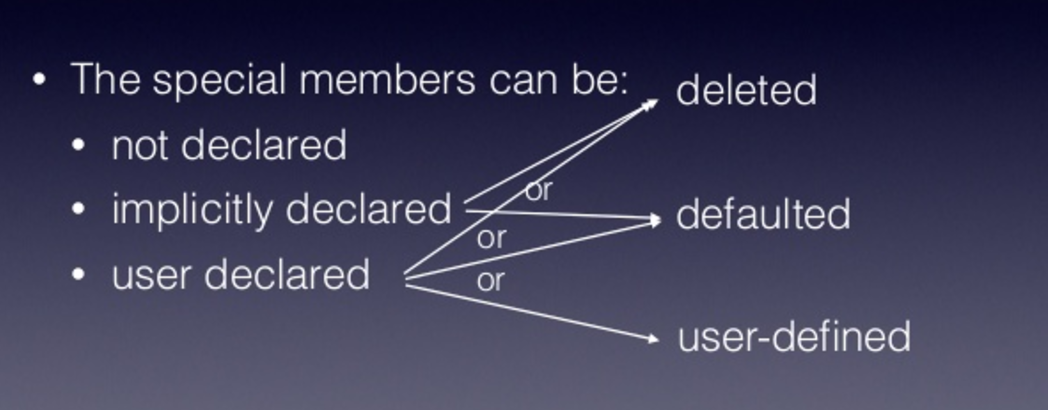
\includegraphics[scale=0.6]{pics/sm1.png} 
\end{center}


	\item If you just define a class without any special member function, all six special member functions(One constructor, destructor, copy construtor, copy assignment, move construtor and move assignment) will be declared by compiler implicitly. 

%\begin{center}
%	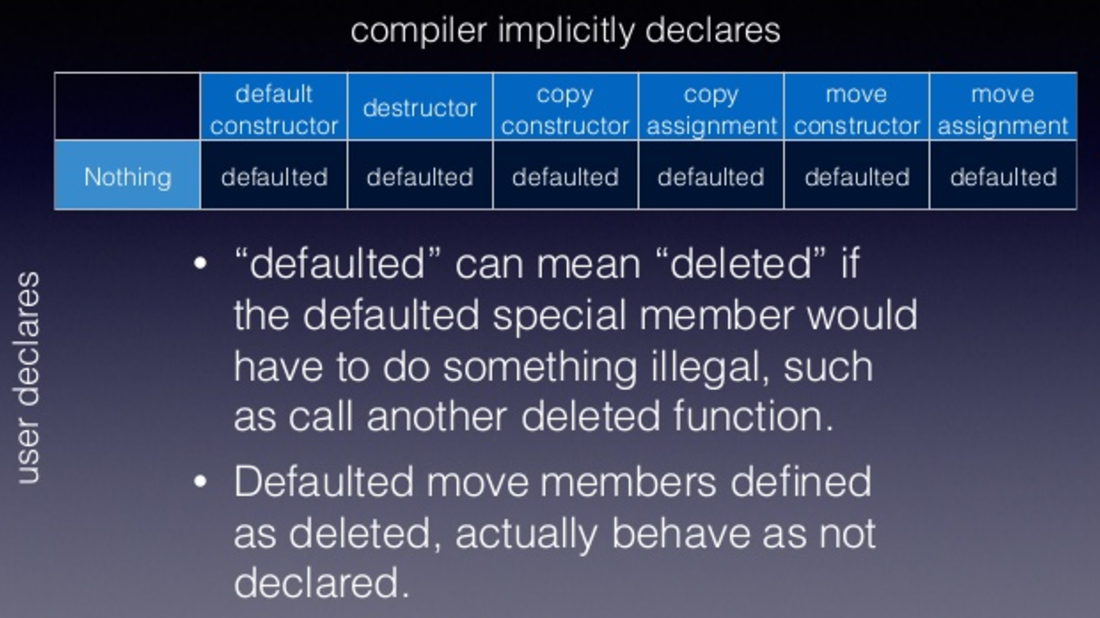
\includegraphics[scale=0.5]{pics/sm2.png}
%\end{center}

	\item "Defaulted" can mean "deleted" if the defaulted special member would have to do something illegal, such as call another deleted function. "default" in \texttt{B} just tell compiler that I want to use compiler's version, and compiler version generate "delete" default constructor for class \texttt{B}. See an example below: 

\begin{lstlisting}[frame=single, language=c++]
class A{
	A() = delete;
};
class B{
	B() = default; 
	A a;
};
int main(){
	B b; //output: 'B::B()' is implicitly deleted because the
}	     // default definition would be ill-formed:       
\end{lstlisting}

    \item Steps of generating special member function. 
\begin{center}
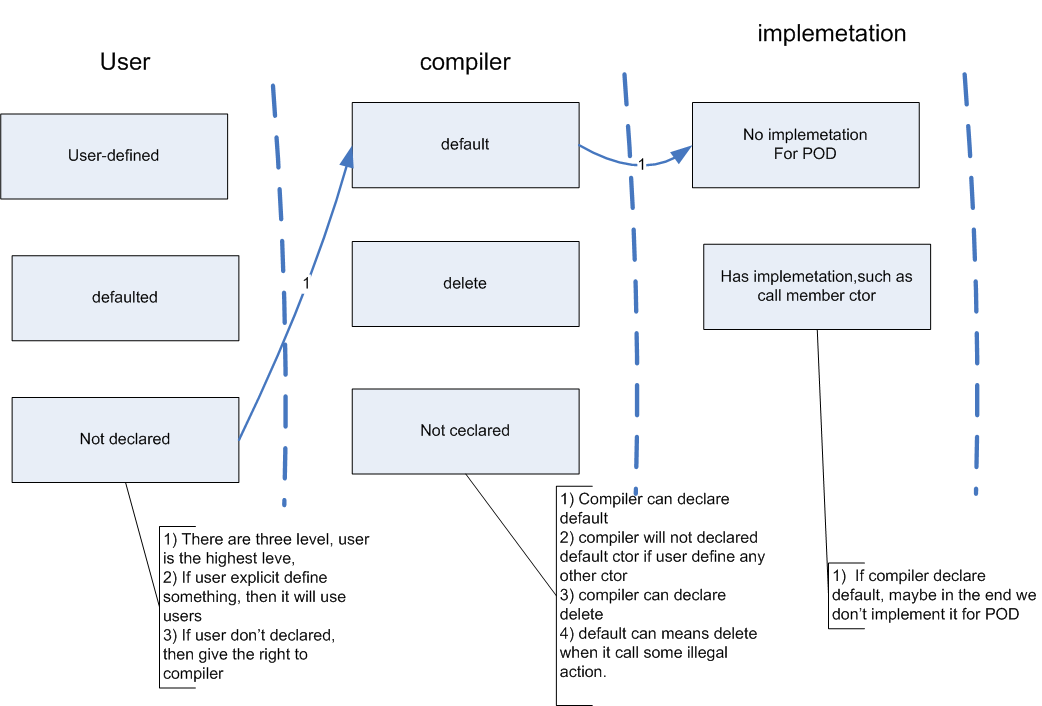
\includegraphics[scale=0.8]{pics/ctor.png} 
\end{center}

	\item Next question is what differences are between \verb|=default| and user define empty constructor? problems of below code snippet are:
	
\begin{lstlisting}[numbers=none]
struct noncopyable  {
	noncopyable() {};
private:
	noncopyable(const noncopyable&);
	noncopyable& operator=(const noncopyable&);
};
\end{lstlisting}
\begin{enumerate}
	\item The copy constructor has to be declared privately to hide it, but because it's declared at all, automatic generation of the default constructor is prevented. You have to explicitly define the default constructor if you want one, even if it does nothing.

	\item Even if the explicitly-defined default constructor does nothing, it's considered non-trivial by the compiler. \textbf{It's less efficient than an automatically generated default constructor and prevents noncopyable from being a true POD type.}

	\item Even though the copy constructor and copy-assignment operator are hidden from outside code, the member functions and friends of noncopyable can still see and call them. If they are declared but not defined, calling them causes a linker error.

	\item Although this is a commonly accepted idiom, the intent is not clear unless you understand all of the rules for automatic generation of the special member functions.
\end{enumerate}

	\item C++11 new keyword default and delete give below advantages:
\begin{lstlisting}[numbers=none]
struct noncopyable  {
  noncopyable() =default;
  noncopyable(const noncopyable&) =delete;
  noncopyable& operator=(const noncopyable&) =delete;
};
\end{lstlisting}

\begin{enumerate}
	\item Generation of the default constructor is still prevented by declaring the copy constructor, but you can bring it back by explicitly defaulting it.

	\item Explicitly defaulted special member functions are still considered trivial, so there is no performance penalty, and noncopyable is not prevented from being a true POD type.

	\item The copy constructor and copy-assignment operator are public but deleted. It is a compile-time error to define or call a deleted function.

	\item The intent is clear to anyone who understands \texttt{=default} and \texttt{=delete}. You don't have to understand the rules for automatic generation of special member functions.
\end{enumerate}

	\item Another question is what the differences are between using \texttt{=delete} and not declaring a member at all. Deleted members participate in overload resolution, while members that are not declared do not participate in overload resolution.
\begin{lstlisting}
struct X{
	template<class ...Args>
		X(Args&& ...args);
	X() = delete
};

X x; //without line 4, here will call template function in line 2.
     //with line 4, compiler will report error here.
\end{lstlisting}

    \item It's preferable to use deleted functions instead of privately undefined ones. Any function, including non-member functions and template instantiations, can be declared as \texttt{= deleted}.

\begin{lstlisting}[frame=single, language=c++]
template <class charT, class traits = char_traits<charT> >
class basic_ios : public ios_base {
public:
	basic_ios(const basic_ios& ) = delete;
	basic_ios& operator=(const basic_ios&) = delete;
};

bool isLucky(int number); // original function
bool isLucky(char) = delete; // reject chars
bool isLucky(bool) = delete; // reject bools

template<typename T>
void processPointer(T* ptr);

template<>
void processPointer<void>(void*) = delete; //can't use void to instantiate.
\end{lstlisting} 

%    \item Why defaulted move member sometimes "deleted"? Detail can be found in "CWG 1402 is (imho) the most important bug fix to C++11". Another good article is google "Why is the move constructor neither declared nor deleted with clang? " In clang, it support C++11 standard better. 
    
%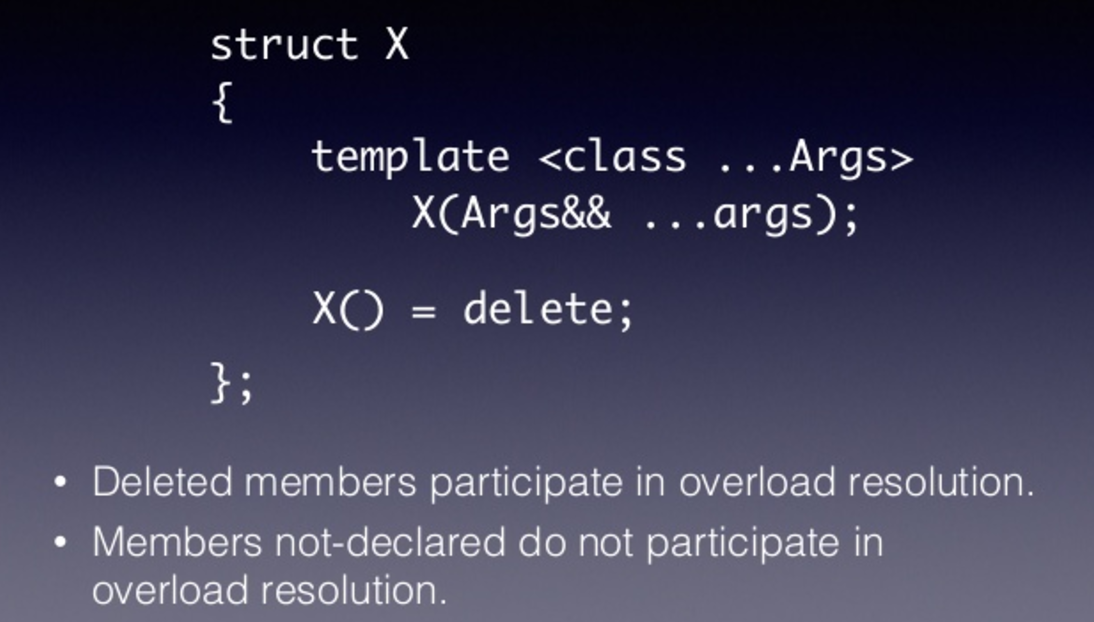
\includegraphics[scale=0.6]{pics/sm5.png} \newline

\end{itemize}

\subsubsection{Rules of implicitly declare }
\begin{itemize}
	\item The Default constructor, will not be implicitly generated if:
	
		\begin{enumerate}
			\item you have explicitly declared any constructor.  Compiler doesn't create a default constructor if we write any constructor even if it is copy constructor.
		
			\item There is a member in your class that is not default-constructible (such as a reference, a const object, or a class with no or inaccessible default constructor)
		
			\item (C++11) you have explicitly told the compiler to not generate one using A() = delete;
		\end{enumerate}

	\item The copy constructor, will not be implicitly generated if:
		\begin{enumerate}
			\item you have explicitly declared a copy constructor (for class X a constructor taking X, X\& or const X\&)
			
			\item there is a member in your class that is not copy-constructible (such as a class with no or inaccessible copy constructor)
			
			\item (C++11) you have explicitly told the compiler to not generate one using A(const A\&) = delete;
		\end{enumerate}


	\item The Copy Assignment Operator will not be implicitly generated if
		\begin{enumerate}
		\item you have explicitly declared a copy-assignment operator (for class X an operator = taking X, X\& or const X\&) )
		\item there is a member in your class that is not assignable (such as a reference, a const object or a class with no or inaccessible assignment operator)
		\item (C++11) you have explicitly told the compiler to not generate one using A\& operator=(const A\&) = delete;
		\end{enumerate}
	
	
	\item The Destructor will not be implicitly generated if 1) you have explicitly declared a destructor. 2) (C++11) you have explicitly told the compiler to not generate one using \textasciitilde A() = delete;

	
	\item The Move Constructor or Move Operator(C++11) will not be implicitly generated if
		\begin{enumerate}
		\item you have explicitly declared a move constructor or move assignment(for class X, a constructor taking X\&\&)
		\item there is a member in your class that cannot be moved (have deleted, inaccessible, or ambiguous)
		\item you have defined a copy assignment operator, copy constructor, destructor, or move assignment operator
		\item you have explicitly told the compiler to not generate one using A(A\&\&) = delete;
		\end{enumerate}
	
	
	\item The Move Assignment Operator (C++11) will not be implicitly generated if
		\begin{enumerate}
		\item you have explicitly declared a move assignment operator (for class X, an operator = taking X\&\&)
		
		\item you have defined a copy assignment operator, copy constructor, destructor, or move constructor.
		
		\item you have explicitly told the compiler to not generate one using A\& operator=(A\&\&) = delete;
		\end{enumerate}
	
	\item  The justification is that declaring a copy operation (construction or assignment) indicates that the normal approach to copying an object(memberwise copy) isn't appropriate for the class, and compilers thinks that if memberwise copy isn't appropriate for the copy operations, memberwise move probably isn't appropriate for the move operations either. The same idea as the previous item, declaring a move operation (construction or assignment) in a class causes compilers to disable the copy operations.
	
	\item The two copy operations(copy constructor and copy assignment) are independent: declaring one doesn't prevent compilers from generating the other. The two move operations are not independent. If you declare either, that prevents compilers from generating the other.
	
	\item C++11 deprecates the automatic generation of copy operations for classes declaring copy operations or a destructor. If you declare a destructor, declare your copy members too, even thought not necessary. This means that if you have code that depends on the generation of copy operations in classes declaring a destructor or one of the copy operations, you should consider upgrading these classes to eliminate the dependence.  Provided the behavior of the compiler-generated functions is correct (i.e, if memberwise copying of the class's non-static data members is what you want), your job is easy, because C++11's "= default" lets you say that explicitly:
		
	\item A summary of previous rules is illustrated in below figure. 
	\begin{center}
		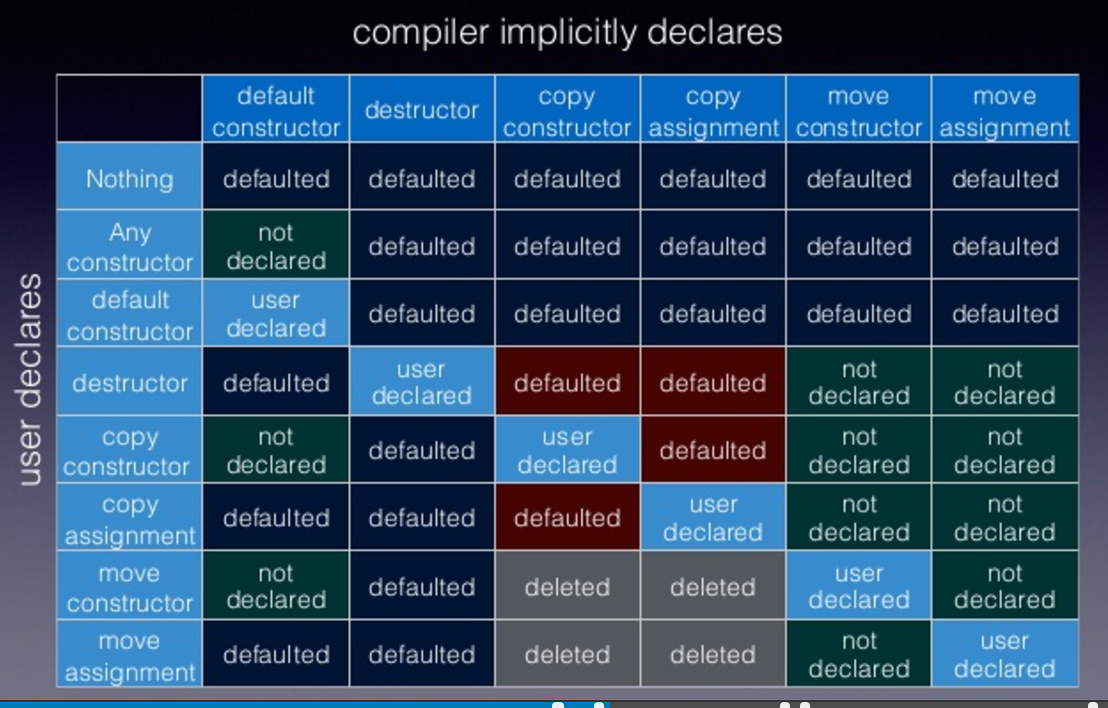
\includegraphics[scale=0.6]{pics/sm3.png}
	\end{center}

	
%\begin{center}
%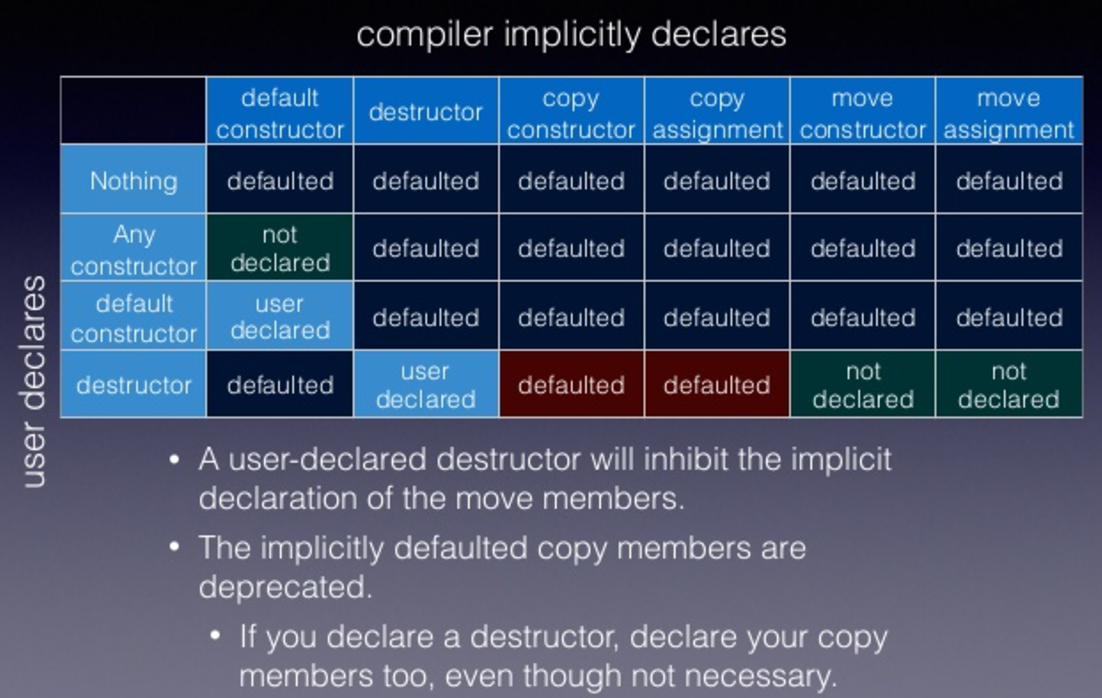
\includegraphics[scale=0.6]{pics/sm4.png} \newline
%\end{center}



\end{itemize}

\subsection{Resource management policy}
\begin{itemize}
    \item If a class only includes value-like members, we usually don't need a resource management policy. In other words, we don't have to build any copy or move constructors; we can just use the compiler-generated default ones. This is known as the \textbf{Rule of Zero}.
\begin{lstlisting}
class NoResource{
	value-like member1; // such string s, std::vector
	value-like member2; // such as int i;
}
\end{lstlisting}

    \item If a class includes reference-like member, things becomes a little complex. You need to consider ownership And lifetime control. We can use \textbf{Four and half rule}, which will be introduced later.

\begin{lstlisting}
class OneRef{
	reference-like member1; //such as a handle, and pointer to a member.
}
\end{lstlisting}

\end{itemize}

\subsubsection{Rule of zero}
\begin{itemize}
    \item Rule of zero: If you can avoid defining default operations, do! It’s the simplest and gives the cleanest semantics. If all members have all the special functions, no further work is needed. In another word, any time you have resource, you can put it into the wrapper and change it into value-like member, in this way, we can follow Rule of zero.

\begin{lstlisting}
class ZeroRule{
	unique_ptr<Foo> p; //don't use Foo* p;
	shared_ptr<Foo> p; //for shared ownership;
	string s;  //don't use char* p;
	vector<int> v; //don't use int* p;
	array<int> a; //don't use int *p;
	std::unique_ptr<void, decltype(&::FreeLibrary)> handle; //don't use HMODULE handle;
}	
\end{lstlisting}

	\item A variant of Rule of zero: As long as you can, stick to the Rule of Zero, but if you have to write at least one of the Big Five, default the rest. Why?  When you "user declare" destructor, according to our previous introduction, it loses its move operations. BUT it doesn’t lose its copy operations! So client code will continue to compile, but will silently call copy instead of move. This is not good. Default version is just like you move member manually, but \texttt{= default} permits you to skip the body definition. 
	 
\begin{lstlisting}
class X{
public:
	X(X const& other) = default;
	X& operator=(X const& other) = default;	
	X(X&& other) = default;
	X& operator=(X&& other) = default;
	~X() { /* log something in the dtor */ }
};
\end{lstlisting}

\begin{lstlisting}
struct Example { 
	string a, b;
	Example(Example&& mE) = default;
	// the same Example(Example&& mE) : a{move(mE.a)}, b{move(mE.b)} { }
}	

\end{lstlisting}
   
    \item Whenever possible, you should consider following the Rule of Zero first. If there isn't a suitable wrapper class, such as \texttt{std::unique\_ptr} or \texttt{std::shared\_ptr}, to meet your requirements or you want to manage your resources yourself, then you can follow the Rule of Four and a Half. The Rule of Four uses the "copy and swap idiom," so I will introduce that first and then move on to the Rule of Four and a Half.

\end{itemize}

\subsubsection{copy and swap idiom, rule of four and half.}
\begin{itemize}
	\item Any class that manages a resource (a wrapper, like a smart pointer) needs to implement The Big Three. While the goals and implementation of the copy-constructor and destructor are straightforward, the copy-assignment operator is arguably the most nuanced and difficult. How should it be done? What pitfalls need to be avoided?
	
	\item The old implementation need 1) avoid assignment self 2) return *this reference. There are two problems, the first one is the old implementation is not strong exception safe. For example, when we copy the content1, an exception has been thrown. Under such context, original one has been damaged. The second problem is so many duplicated code. The assignment code has almost the same code with copy constructor.
\begin{lstlisting}[numbers=none]
class & class::operator=(class &a){
	if(this == &a)
		return *this;  //avoid assign by himself
    this.content1 = a.content1; //
    this.content2= a.content2; 
	return *this ; // return *this reference.
}	
\end{lstlisting}
	
	\item The copy-and-swap idiom is a better solution, and elegantly assists the assignment operator in achieving two things: avoiding code duplication, and providing a strong exception guarantee. Conceptually, it works by using the copy-constructor's functionality to create a local copy of the data, then takes the copied data with a swap function, swapping the old data with the new data. The temporary copy then destructs, taking the old data with it. We are left with a copy of the new data. In order to use the copy-and-swap idiom, we need three things: a working copy-constructor, a working destructor (both are the basis of any wrapper, so should be complete anyway), and a swap function. The swap function can be a member function.
	
    \item A low efficient implementation with swap. We should not use reference as function parameter. \textbf{No matter lvalue or rvalue, copy always happen inside assignment operator.}
\begin{lstlisting}[numbers=none]
dumb_array& operator=(const dumb_array& other){
	dumb_array temp(other);
	swap(*this, temp);
	return *this;
}	

dumb_array da;
da = f(); // use const & get the pvalue, // but inside the operator =, we copy. 
// we didn't use move, so it's low efficient.	
\end{lstlisting}
	
	\item  A efficient way is to use value parameter. On a general note, a remarkably useful guideline is as follows: if you're going to make a copy of something in a function, let the compiler do it in the parameter list.
	
\begin{lstlisting}[numbers=none]
dumb_array& operator=(dumb_array other){
	other.swap(*this); 
	return *this;
}	

dumb_array da;
da = f(); // use move directly. high efficient.
\end{lstlisting}
	

\item The full code is here: 
\begin{lstlisting}[]
class dumb_array{
	dumb_array(const dumb_array& other): mSize(other.mSize),
			mArray(mSize ? new int[mSize] : nullptr){
		std::copy(other.mArray, other.mArray + mSize, mArray);
	}
	dumb_array(dumb_array&& other):dumb_array{} noexcept{
		*this.swap(other);
	}
	void swap(dump_array& rhs) noexcept{
		using std::swap;
		swap(msize, rsh.msize);
		swap(mArray, rsh.mArray);
	}
	dumb_array& operator=(dumb_array other) noexcept{
		other.swap(*this); 
		return *this;
	}
private:
	std::size_t mSize;
	int* mArray;
};

void swap(dumb_array& first, dumb_array& second) {
	first.swap(second);
}
namespace std{
	template<> 
	void swap<dump_array>{dump_array& first, dump_array& seconde){
			first.swap(second);
		}
} 
\end{lstlisting}
\begin{description}
    \item[Line 9:] Why do we need member swap? because it can visit private member of class. So swap in line 9 may not be declare friend. That is a good style. Inside swap member function, you may use std::swap to exchange class member and label it noexcept.
    
	\item[Line 14:] Use swap member function to implement assignment operator, the function parameter is value, and label it noexcept. 
	
	\item [Line 18:] Once we have swap functions, we can use it to implement move constructor and label it noexcept. That is very important, when we use \texttt{vector<dump\_array>}, when vector need expand its size, it will use move if move is noexcept, if move is not noexcept, it will use copy which deep copy happens. 
    
    \item[Line 26:] If \texttt{dump\_array} has it's own namespace, then put swap non-member swap function into the same namespace. In this way, client can use ADL find this version and pick it up. If no own namespace, just put it in global scope.
    
\begin{lstlisting}
namespace_dr::dumb_array dr1;
namespace_dr::dumb_array dr2;
swap(dr1, dr2); // will go to namespace_dr to find the correct swap function.
\end{lstlisting}

    \item [Line 29:] You also need to put swap into the std namespace and make it specialization.
\begin{lstlisting}
//clients code should be like this
using std::swap
swap(dr1, dr2);  //using your version.
std::swap(dr1,dr2) //some people or STL library code will use this way
                   //also guarantee that your version can be called properly. 
\end{lstlisting}	

\end{description}
	
	\item An interesting example about copy and swap idiom.  For below software snippet, copy and swap idiom is slow than the default empty \texttt{X}. Why? Detail can be found in "Inefficiency of copy-and-swap idiom?" in stack overflow. In another word, don't use "copy and swap" on some std container member, because \texttt{std::vector<int>} has been value like member. 
\begin{lstlisting}
class X{  //
	std::vector<int> v_;
}

class X{ //copy and swap idiom
	std::vector<int> v_;
	X& operator=(X x){
		v_.swap(x.v_);
		return *this;
	}
}
\end{lstlisting}

	\item If we need a user-defined copy constructor to avoid shallow copy, and at the same time, we need a user-defined destructor to free or release some resources, that is a strong indication that we can use the "four and a half idiom". In the previous code snippet, Class X doesn't need its own copy constructor and destructor, wo we should NOT use "four and a half idiom" here either. 


	\item Before C++11, we didn't have move semantics, so we just needed to follow the Rule of Three: If a class requires a user-defined destructor, a user-defined copy constructor, or a user-defined copy assignment operator, it almost certainly requires all three. After C++11, with the introduction of move semantics, the Rule of Three became the Rule of Five, adding a move constructor and a move assignment operator.
	
	\item With help "copy and swap idiom", the rule of five becomes to the Rule of The Big Four (and a half), which states that if you implement one of below file, you should implement all the others.
	\begin{enumerate}
		\item The copy constructor.
		\item The assignment operator. Don't need move assignment, in assignment operator, we pass only one kind of type--value. 
		\item The move constructor.
		\item The destructor.
		\item The swap function(that is half).
	\end{enumerate}
    	
\end{itemize}

\subsubsection{Summary}
\begin{itemize}
    \item For non-resource classes, you should follow the zero rule. For classes that wrap resources, you should follow the four and a half rule. Don't use the big three rule, as it has been deprecated after C++11.

    \item You can use \texttt{=default} and \texttt{=delete} to explicitly declare some special member functions. For example, if you define destructor for log purpose, it will disable copy constructor generation, at this time, you can add \texttt{Foo Foo(cont Foo\& rhs)=default} to your class to bring them back.
        
    \item The common use resource management policies are below:
\begin{enumerate}
    \item Objects that can be both moved and copied
    \item Objects for which it makes sense to copy but not move
    \item Objects for which it makes sense to move but not copy
    \item Objects which should neither be moved not copied.
\end{enumerate}

	\item Besides these famous idiom, you can customize your own class management policy. Different policy will make the class has different behavioral, then represents the practical application semantic the best. 
	
	\begin{enumerate}
		\item Use the compiler-provided versions of these functions. In other words, you're not doing any resource management in the class.
		
		\item Write your own move functions, but don't support copying, such as \texttt{std::unique\_ptr}
		
		\item Disable copying and move semantics for the class, because it doesn't make sense to allow it, such as \texttt{std::mutex}
		
		\item For \texttt{std::unary\_function}, it's base class, but it's just trait class.(extract type information from a function). You can declare its destructor as protect and non virtual. Then your client can't use below code:
\begin{lstlisting}[numbers=none]
class Base {
protected:
	~Base(){
		cout<<"Base::Destructor\n";
	}
};

Base *base_ptr = new Base{};
delete base_ptr; //compiler barks here.
\end{lstlisting}
	\end{enumerate}

\end{itemize}

\subsection{operator overload}
\begin{itemize}
	\item Overload means providing two (or more) functions that perform similar, closely related things, differentiated by the types and/or number of arguments it accepts.
	
	\begin{enumerate}
		\item  In some cases it's worth arguing that a function of a different name is a better choice than an overloaded function.
		
		\item  In the case of constructors and operator, overloading is the only choice because we can't give them the different name. and operator overload is typical feature in Object Base Programming.(OB)
		
		\item Sometimes, overload and default parameter have same client usage, as shown below. If there is a value that you can use for a default, use default parameter. Overload usually take different parameter type or different number of parameters.
\begin{lstlisting}[numbers=none]
void f();
void f(int x);
f() or f(10);

void g(int x = 0);
g() or g(10);	
\end{lstlisting}				
	\end{enumerate}

	\item \textbf{Never overload \&\&, || and comma in C++.  Just remember it!}
	
	\item For all operators where you have to choose to either implement them as a member function or a non-member function, use the following rules of thumb to decide:
	\begin{enumerate}
		\item If it is a unary operator, implement it as a member function.
		
		\item If a binary operator treats both operands equally (it leaves them unchanged), implement this operator as a non-member function.
		
		\item If a binary operator does not treat both of its operands equally (usually it will change its left operand), it might be useful to make it a member function of its left operand’s type, if it has to access the operand's private parts.
		
		\item If you both define member and nonmember operator, it will call your member version first,  If you delete the member version, then it will call nonmember version. 
\begin{lstlisting}
class Sample{
public:
	Sample operator + (const Sample& op2){ return Sample{};}
	friend Sample operator + (const Sample& op1, const Sample& op2);
};

Sample operator + (const Sample& op1, const Sample& op2){
	return Sample{};
}
Sample s1{};
Sample s2{};
Sample s3 = s1+s2;  //this line call member version in line 3. 
\end{lstlisting}

	\end{enumerate}
	
	
	\item You can declare operator as member function. if it's not member function, declare it as a friend function if it need to visit private member variable. If you want to overload + operator, and support time t; 3+t;   You need to define a friend function. In order to improve a \texttt{t+3} efficiency, you also can define a member function time \texttt{operator+(int i)} member function.
\begin{lstlisting}[frame=single, language=c++]
time operator+(const time &lhs, const time &rhs); //non-member function
friend time operator+(int,  const time &t) //nonmember, for 3+t;
time operator+(int i) //member, for t+3, avoid implicit conversion from 3 to t
\end{lstlisting}

	\item Overloading sometimes can help you to avoid implicit type conversion. In the below example, we avoid creating a temporary obj implicitly created by constructor.

\begin{lstlisting}[frame=single, language=c++]
 class String{
	bool operator==(const String& lhs, const String& rhs);
}
String str;
if(str =="hello") //will build a temp obj String("hello");

bool operator==(const String& lhs, const char* rhs); //avoid implicit conversion.	
\end{lstlisting}

	
	\item When implementing binary arithmetic operators such as +, -, and *, it's good practice to first implement compound assignment operators such as +=, -= and *=. These can then be used to implement the common operators. For example, you can use += to implement +. This design provides two advantages: 1) it provides an additional function, and 2) it avoids code duplication. 
\begin{lstlisting}[numbers=none]
Vector2D& Vector2D::operator+=(const Vector2D& right){
	this->x += right.x;
	this->y += right.y;
	return *this;
}

Vector2D operator+(const Vector2D& lhs, const Vector2D& rhs){
	Vector2D result = lhs;
	result += rhs;
	return result;
}
\end{lstlisting}
	
	\item Why does \texttt{<<} need to be both a friend and a non-member? Its left operands are stream classes from the standard library, which cannot be changed. In other words, you need to write \texttt{cout << obj}. If you declare \texttt{<<} as a member operator, you would have to write \texttt{obj << cout}, which looks weird.
	
	\item The assignment operator overload should return a non-const reference. Some people suggest that returning a const reference can avoid the possibility of writing code like (x=y)=z. However, this is not a common coding practice. In the STL string, the assignment operator just returns a reference. This serves as a helpful reminder that whenever you have questions about interface design, you can look to the STL library for guidance.
\begin{lstlisting}[numbers=none]
class A & operator=(const class A& rhs){	
	//Do some things other
	return *this;
}
\end{lstlisting}

	\item The binary operators = (assignment), [] (array subscription), -> (member access), as well as the unary () (function call) operator, must always be implemented as member functions, because the syntax of the language requires them to.
	
\end{itemize}


\section{Object oriented}

\subsection{Inheritance}
\subsubsection{Polymorphism by inheritance}

\begin{itemize}
	\item Polymorphism is a powerful design mechanism that allows for the encapsulation of related types behind an abstract public interface. However, the cost is an additional level of indirection, both in terms of memory acquisition and type resolution. This style of programming is called object-oriented programming. Polymorphism is supported only by references and pointers. See the source code below:

\begin{lstlisting}[numbers=none]
class A{
public:
	virtual void fun(){ cout<<"A";}
};
	
class B: public A{
public:
	void fun(){cout<<"B";}
	int m_b = 100;
};
\end{lstlisting}

	\item Base pointer can't access class member in derived class directly.
	
\begin{lstlisting}
B b;
A* pa = &b;
cout<<b.m_b;    //OK,You can access class member by object directly.
//cout<<pa->m_b;   //ERROR 
//cout<<(*pa).m_b; //ERROR
cout<<static_cast<B*>(pa)->m_b; //OK
\end{lstlisting}
\begin{description}
	\item[Line 4-5:] Error, it doesn't work. Pointer has type. The pointer type alter the interpretation of the size and composition of the memory. Pointer type is \texttt{A}, so the size of memory which pointer address is sizeof(A), that's why you can't see the \texttt{m\_b} at all.
	\item[Line 6:] OK, when you change the pointer type from A to B, then the memory which pointer address is \texttt{sizeof(B)}, interpretation also support \texttt{->m\_b} now. 
\end{description}

\item Base object doesn't support polymorphism.
\begin{lstlisting}
B b;
A a = b; //sliced happen here.
a.fun(); //output A
\end{lstlisting}
\begin{description}
	\item[Line 2:] When a base class object is directly initialized or assigned with a derived class object, the derived object is sliced to fit into the available memory resources of the base type. Virtual table content changed. There is nothing of the derived type remaining. 
	
	\item[Line 3:] Polymorphism is not present, and an observant compiler can resolve an invocation of a virtual function through the object at compile time, thus by-passing the virtual mechanism.
\end{description}

	\item A pointer or a reference support polymorphism because in derived class, we build virtual table, (adding indirect level.)
\begin{lstlisting}
A& ra = b;
ra.fun(); //output B
A* pa = &b;  no sliced happen here
pa->fun(); //output B
(*pa).fun(); //output B, no sliced happen before.
		
A* pa1 = new B; //virtual table content has not changed.
(*pa1).fun(); //output B
\end{lstlisting}

\end{itemize}

\subsection{Member functions in inheritance}

\subsubsection{constructor and destructor in inheritance}
\begin{itemize}
	\item  \textbf{The subclass constructor will always call the base class constructor.} The idea behind this rule is to ensure that an object can be initialized properly. The constructor should NOT be virtual. If the subclass doesn't define any constructor, the compiler will implicitly define a default constructor, and this constructor will call the base class's default constructor. If the subclass has a constructor but doesn't explicitly call the base class's specified constructor, the constructor of the subclass will call the base class's default constructor (without any parameters). If the base constructor only has a specified constructor and no default constructor, the compiler will produce an error. If you want to explicitly call the base class's specified constructor, use the initialization list syntax.
\begin{lstlisting}[frame=single, language=c++]
class base{
public:
	base();  //default constructor
	base(int b); //converting constructor
	private:
	int b;
};
	
class subclass: public base{
	subclass();  //default constructor
	subclass(int s, int b); // converting constructor1
	subclass(int s);     //converting constructor2
	int s;
};
	
subclass::subclass(int s, int b): base(b){
	m_s = s;
}
//////////////////////////////////////////
subclass sc1(2,3); //call converting constructor, explicit call base constructor constructor.
subclass sc2(2);  // implicit call base default constructor
subclass sc3;   //if base has no default constructor, sc2 and sc3 report error
\end{lstlisting}

	\item If you don't use explicit initialization list syntax to call the base class's specified constructor, you will either get an uninitialized value or you won't be able to initialize the base member, both of which are not good.
\begin{lstlisting}[frame=single, language=c++]
DeriveClass::DeriveClass(int base_a, b){ // call default constructor,  
	Derive_b = b
}	

DeriveClass::DeriveClass(int base_a, b) {
	base_a = a  //It can be thought as a bad design.
	Derive_b = b
}
\end{lstlisting}
\begin{description}
	\item[Line 1:] it will call \texttt{base\_class} default constructor. in this case, \texttt{base\_a} is not assigned at all.
	\item[Line 6:] You can't access private base member data. \texttt{base\_a} need to be public member data.
\end{description}

	\item If a base class has a destructor, but sub class doesn't have, compiler will produce an implicit default destructor, and this implicit default destructor will call base class destructor. If you define a subclass destructor, It will call base destructor automatically, you don't need to call it explicitly. The question is, How can you make sure you sub class destructor will be called if you use a base class pointer or reference? You need to make the base class destructor virtual. That introduce an important principle: \textbf{Make base class destructor public and virtual} (polymorphic deletion by base class pointer or reference), or protect and non-virtual, base classes need not always allow polymorphic deletion. For example, consider class templates such as \texttt{std::unary\_function}. This time, you should make destructor protected and non-virtual.
\begin{lstlisting}[]
template <class Arg, class Result>
struct unary_function{
	typedef Arg    argument_type;
	typedef Result result_type;
};
	
void f( std::unary_function* f ){
	delete f; // error, illegal code to use unary_function in this way.
}
\end{lstlisting}
\begin{description}
	\item[Line 8:] Make destructor protected and non-virtual, then this line will compile with failure, it's good design. 
\end{description}

	\item Don't call base destructor explicitly, It will called automatically in the reverse order of construction.  And you should give a base destructor a definition, Or linker will report error it even you don't call it in your source code.
	
	\item Never throw an exception from a destructor. If exception A is thrown, then stack unwinding will occur. When an object is destructed, its destructor is called, and if another exception B is thrown by the destructor, the application will call the terminate function immediately. If you encounter an exception, catch it inside the destructor.
	
\end{itemize}

\subsubsection{copy constructor in inheritance}

\begin{itemize}
	\item Copy constructor(assignment constructor) in inheritance sometimes causes \textbf{slicing problem}.   Below five are all SLICING problems, number 4 and number 5 is not very obvious. They all call base class constructor.  No matter what you input a reference to a derived class or not.
\begin{lstlisting}[numbers=none]
class Base{};
class Derived1 : Base{};
class Derived2 : Base{};
Derived1 d1;
Derived1 d2;
/////////////////////
Base b = d1; //1)
	
Fun(Base b);
Fun(d1);  //2)
	
Base& Bref = d1;
Fun(Bref) //3)
	
Base* bp = new Base(Bref); //4) call base copy constructor
	
Base* bp1 = new Derived1();  //5) sibling slicing
base* bp2 = new Derived2();
*bp1 = *bp2;  // bp1 just copy Base part in Derived2.
//so bp1 now is MIXTURE of d1 and d2.
\end{lstlisting}

%	\item What does a typical user defined move constructor do?
%\begin{lstlisting}[numbers=none]
%class Child : public Base{
%	Member m_;
%	Child(Child&& x): Base(std::move(x)), m_(std::move(x.m_)){
%		x.set_to_resourceless_state();
%	}
%}
%\end{lstlisting}
	
	
\item Think a problem as below: how to make deep copy and avoid slicing in base class copy constructor?
\begin{lstlisting}[numbers=none]
class Base{};
class Derived1 : Base{};
class Derived2 : Base{};
Derived d1;
Derived d2;
	
Base* Copy(Base& Bref){
	//How to avoid slicing and make deep copy here?
}
	
Base& Bref = d1
Base* d1p = Copy(Bref)

Base& Bref = d2
Base* d2p = Copy(Bref)
	\end{lstlisting}
	
\item Continue- Think this problem: error method
\begin{lstlisting}[numbers=none]
Base* Copy(Base& Bref){
	Base* p = new Base(Bref) //Slicing happen here, error!
}
\end{lstlisting}
	\item Continue- Think this problem: TypeID method.
\begin{lstlisting}[numbers=none]
Base* Copy(Base& Bref){
	int typeid;
}
\end{lstlisting}
\begin{description}
	\item[Line 2:] Use \texttt{type\_id} and \texttt{dynamic\_cast}. involve a lot of if and switch about type. anytime if you use \texttt{dynamic\_cast} and \texttt{if}, you can think about using virtual function instead.
\end{description}
	
\item Continue- Think this problem: Virtual Clone method.
	A function's return type is never considered part of its signature. You can override a member function with any return type as long as the return type could be used wherever the base class return type could be used.
\begin{lstlisting}[numbers=none]
class Base{
	virtual Base* Clone() = 0;
};
	
class Derived1 : Base{
	virtual Derived1* Clone(){return new Derived1(*this);}
}
	
Base* Copy(Base& Bref){
	Base* p = Bref.Clone();
}
\end{lstlisting}
	
	\item Continue- Think this problem: Change Design. Base is concrete class,  More Effective C++ Item 33 said "Making Non-leaf class abstract". So maybe you can change the inheritance system design.
	
	\item Assignment operator and copy constructor in inheritance summary:

	\begin{enumerate}
		\item Default Assignment  operator and  copy constructor in derived class which are implicitly produced by compiler will call default base assignment operator and copy constructor.
		
		\item If derived class has no new operation. Don't need to define derived class Assignment operator and  copy constructor, implicit one will call base one automatically.
		
		\item If derived class has new operation. You have to define derived class Assignment  operator and  copy constructor, it will NOT invoke assignment  operator and  copy constructor in base class any more.  Inside, manually invoke base class Assignment operator and copy constructor. Detail can be found in C++ primer p760. Syntax looks like below: see effective C++ Item 16.
		
		\item For copy constructor, just initialization list syntax. For assignment operator, use two different methods depends on if base class declare its own assignment operator(). Source code is below:
		
\begin{lstlisting}[frame=single, language=c++]
DerivedClass::DerivedClass(const DerivedClass &dc): \
	BaseClass(dc){...}  //init list syntax here.
		
DerivedClass & DerivedClass::operator=(const DerivedClass &dc){
    BaseClass::operator=(dc);
    ( (BaseClass&) *this ) = dc
    ( (BaseClass) *this ) = dc // this will call baseclass copy constructor.
}
\end{lstlisting}

\begin{description}
	\item[Line 5:] If base class declare explicitly operator, we can call it explicitly.
	\item[Line 6:] Base class no explicitly operator, change \texttt{*this} to \texttt{BaseClass} reference, if you change to \texttt{BaseClass}, It will call copy constructor.
\end{description}
		
	\end{enumerate}

	\item For conversion constructors and destructors, the derived class always calls the base class one. Even if you define your own constructor or destructor, it will also implicitly call the base class one. However, for copy constructors and assignment operators, the derived class's implicit constructor or operator will not call the base class one. If you define your own copy constructor or assignment operator, you need to manually call the base class one. This is the difference between conversion constructors and destructors versus copy constructors and assignment operators.

%	\item There are three articles, you should read them together.\\
%\\
%https://herbsutter.com/2013/05/09/gotw-1-solution/
%\\
%https://stackoverflow.com/questions/21825933/any-difference-between-copy-list-initialization-and-traditional-copy-initializat
%\\
%https://stackoverflow.com/questions/1051379/is-there-a-difference-between-copy-initialization-and-direct-initialization

\end{itemize}

\subsection{Virtual function and override}

\begin{itemize}
	\item Almost all base classes have a virtual function. If a class does not contain a virtual function, it is an indication that it is not meant to be used as a base class, except for some base classes that are only intended for injecting a specific type, such as \texttt{unary\_function}.
	
	\item Only virtual functions are included in the vtbl. Friend functions cannot be virtual functions because they are not even members of the class. When a method is declared virtual in a base class, it is automatically virtual in the derived class, but it is still a good idea to explicitly declare it using the keyword \texttt{virtual} in the derived class declarations as well.
	
	\item Do not rewrite non-virtual base member functions. It is not overriding but overwriting. In fact, overwriting is not a standard concept in C++. Most of the time, you can refer to it as \textbf{name hiding}. If you redefine the same non-virtual function name in both the base and child classes, you cannot use dynamic binding, only static binding. 
\begin{lstlisting}[frame=single, language=c++]
class A{
	f(int) {}
};
class B:public class A{
	f(int)  {} // overwrite A::f(int)
};

A* pa = new B();
pa->f(3) // call base f, because pa is A*, event it points to B. 	
\end{lstlisting}

	\item For overriding to occur, several requirements must be met:
	\begin{enumerate}
		\item The base class function must be virtual.
		\item The base and derived function names must be identical (except in the case of
		destructor).
		\item The parameter types of the base and derived functions must be identical.
		\item The constness of the base and derived functions must be identical.
		\item The return types and exception specifications of the base and derived functions
		must be \textbf{compatible}. Don't need to be the same.
		\item To these constraints, which were also part of C++98, C++11 adds one more: The functions' reference qualifiers must be identical. Below code demonstrate reference qualifier usage:
\begin{lstlisting}
class Widget {
public:
	void doWork() &;  //This doWork applies only when *this is an lvalue.
	void doWork() &&; //This doWork applies only when *this is an rvalue.
}; 
	
Widget makeWidget(); // factory function (returns rvalue)
Widget w; // normal object (an lvalue)
w.doWork();  //call Widget::doWork &
makeWidget().doWork();  //call Widget::doWork &&
	\end{lstlisting}

	\end{enumerate}
	
	\item Any small error will not real override base virtual function. But creating a new virtual method with a different signature. such as examples below.

\begin{lstlisting}[numbers=none]
class Base {
public:
	virtual void mf1() const;
	virtual void mf2(int x);
	virtual void mf3() &;
	void mf4() const;
};

class Derived: public Base {
public:
	virtual void mf1();
	virtual void mf2(unsigned int x);
	virtual void mf3() &&;
	void mf4() const;
};
\end{lstlisting}
	
	\item Use the \texttt{override} specifier in derived class member functions to check if they match with the member function in the base class. It can overcome all implicit non-override problems in the previous source code.
\begin{lstlisting}[numbers=none]
struct A{
	virtual void foo();
	void bar();
	virtual void goo(const int);
};
	
struct B : A{
	void foo() override; // OK: B::foo overrides A::foo.
	void bar() override; // Error: A::bar is not virtual.
	void goo(int) override; //Error; different signature. 
}
\end{lstlisting}
	
    \item Use \texttt{final} specifier in Base class, to stop sub-class override.
\begin{lstlisting}[numbers=none]
class Base{
	virtual void method1() final;
}
\end{lstlisting}
	
\end{itemize}

\section{Classes relationship}

\subsection{structure semantic}

\subsubsection{Relationship}

\begin{itemize}
	\item OOP has five relationships:
	\begin{description}
		\item[Composition] Composition exists when a member of a class has a \textbf{part-of} relationship with the class. Compositions are typically implemented via normal member variables or by pointers where the class manages all the memory allocation and deallocation. In semantic level, it involves ownership, the same lifetime, and no change in the middle, such as a person and their head. You should use a composition relationship if possible. To qualify as a composition, an object and a part must have the following relationship:
		\begin{enumerate}
			\item The part (member) is part of the object (class).
			\item The part (member) can only belong to one object (class) at a time.
			\item The part (member) has its existence managed by the object (class).
			\item The part (member) does not know about the existence of the object (class).
		\end{enumerate}
	
	
	
	\item[Aggregations] exists when a class has a \textbf{has-a} relationship with the member. Aggregations are typically implemented via pointer or reference. In semantic level, it has ownership, maybe same life time, may change in the middle,  such as container and pointer(same life time, changeable), airport and airplane and school and teacher. In an aggregation relationship, the class does not manage the existence of the members. To qualify as an aggregation, an object and its parts must have the following relationship:
	
	\begin{enumerate}
		\item The part (member) is part of the object (class)
		\item The part (member) can belong to more than one object (class) at a time
		\item The part (member) does not have its existence managed by the object (class)
		\item The part (member) does not know about the existence of the object (class)
	\end{enumerate}


	
	\item[Associations] are a looser type of relationship, where the class \textbf{uses-a} object. Associations may be implemented via pointer or reference, or by a more indirect means (such as holding the index or key of the associated object).  People and toothbrush(same life time, changeable),  Teacher and student( not same life time, changeable), person and mother(Not Nullity), person and wife( Nullity, no Ownership, different life time), To qualify as an association, an object and an associated object must have the following relationship:
	\begin{enumerate}
		\item The associated object (member) is otherwise unrelated to the object (class)
		\item The associated object (member) can belong to more than one object (class) at a time
		\item The associated object (member) does not have its existence managed by the object (class)
		\item The associated object (member) may or may not know about the existence of the object (class)
	\end{enumerate}


	\item[Dependency] exists when a member of a class has a part-of relationship with the class. In a composition relationship, the class manages the existence of the members. To qualify as a composition, an object and a part must have the following relationship: No Ownership, Not Includes as a member, person and friend.
	\textbf{Dependency definition: If class X's member function argument is class Y, X is dependency of Y.} Dependency definition extension: For a class X, all functions, including free functions, that both "Mention" X and "supplied with" X are logically part of X, because they form part of the interface of X. Supplied with means that they appear in the same header file.


	\item [Inheritance] Main disadvantage: Tightly coupled, fragile, prone to be abused by developers
	\end{description}

	
\begin{center}
	\begin{tabular}{|p{0.25\textwidth}|p{0.12\textwidth}|p{0.12\textwidth}|p{0.15\textwidth}|p{0.15\textwidth}|}
		\tophline 
		 & Composition  & Aggregation  & association & Dependency \\ 
		\tophline 
		Relationship type& Whole/part  & Whole/part  & otherwise unrelated  & otherwise unrelated  \\ 
		\tophline 
		Members can belongs to multi classes& no  & yes & yes & yes  \\ 
		\tophline 
		member existence managed by class& Yes & no & no   & no \\ 
		\tophline 
		Directionality & uni  & uni & uni or bidirectional & uni  \\ 
		\tophline 
		relationship verb& part-of & has-a & uses-a & depends-on 
		\bottomhline 
	\end{tabular}
\end{center}

	\item Composition is specific aggregation, and aggregation is specific associate.

%	\item For Aggregation, It is not a very clearly defined concept and in my opinion it causes more confusion than it is worth. Toothbrush and people can be thought as association relationship more from \textbf{semantic relationship perspective}. composition and association are used more often than aggregation. From \textbf{implementation} perspective,  we can implement divide association into shallow copy and deep copy. 
%	
%	\begin{description}
%		\item[Association-shallow copy:] Foo has a pointer to Bar object as a data member.
%		\item[Association-deep copy:] Foo has a pointer to Bar object and data of Bar is deep copied in that pointer.
%		\item[Composition:] Foo has a Bar object as data member.
%	\end{description}

	\item We can not map relationship in real word into C++ 100\% accurate. C++ is programming language which has its own syntax and semantic understand. Just like we can not inherit ellipse from circle in C++, but we can do this in real word. So we should not treat all the above relationships too pedantically! 

    \item In previous five relationships, inheritance is easy to understand, but is abused the most. I will introduce more deep thought about inheritance. 
	
\end{itemize}

\subsection{Go deeper into inheritance}

\subsubsection{Basic syntactic knowledge about inheritance}

	\begin{itemize}
	
		\item Both references and pointers support polymorphism. In C++ language, you can use inheritance with just the header and library files, without any additional source code.
		
		\item Pure virtual class can't be instance, it just a abstract interface, it's agreement between your class author(developer) and class user(client).
\begin{lstlisting}[numbers=none]
class Shape{
	virtual draw() = 0 
}	//you have to redefine it in your child class
			
class Circle: public Shape{
	...
}
\end{lstlisting}
			
	\item There are three kinds of inheritances. Code and example and explanation:
\begin{lstlisting}[frame=single, language=c++]
class B                    { /*...*/ };
class D_priv : private   B { /*...*/ };
class D_prot : protected B { /*...*/ };
class D_publ : public    B { /*...*/ };
\end{lstlisting}
	
	\begin{enumerate}
		\item None of the derived classes can access anything that is private in B.
		
		\item In \texttt{D\_priv}, the public and protected parts of B are private.
		
		\item In \texttt{D\_prot}, the public and protected parts of B are protected. Protect used in three generation inheritance. By protected Inheritance, grandfather member become protected member in father, so Grandson can still use grandfather's members.
		
		\item In \texttt{D\_publ}, the public parts of  B are public and the protected parts of B are protected (D\_publ is-a-kind-of-a B).
		
	\end{enumerate}

	\item To make a public member of B public in D\_priv or D\_prot, state the name of the member with a B:: prefix. E.g., to make member \texttt{B::f(int,float)} public in D\_prot, you would say:
\begin{lstlisting}[numbers=none]
class D_prot : protected B {
public:
	using B::f;  // Note: Not using B::f(int,float)
};
\end{lstlisting}

    \item If you want to reuse string code in class student(also means \textbf{has-a} relationship, student has a string name) you have two options, The first is composition,  the second is private inheritance.
\begin{lstlisting}[numbers=none]
class Student{ // 1) use composition.
	int getNameLen();
private:
	string m_name;
	vector<double> score;
};

int Student::getNameLen(){
	return m_name.length();
}
\end{lstlisting}

	\item In short, composite uses object names to invoke a method, whereas private inheritance uses the class name and scope resolution operator instead. If you need the base class itself, you can use a type cast such as \texttt{(const string\&) * this}; more details can be found in "C++ Primer," page 800. Using private inheritance is not a mainstream style, so please don't use it unless you are in a corner case.
\begin{lstlisting}[numbers=none]
class Student: private string, private std::vector<double>{//2)private inheritance
	int getNameLen(); // We don't need private member data any more
}
int Student::getNameLen(){
	return string::length(); //use class name and scope-resolution operator
}
const string& Student::getName(){
	return (const string&) *this;
}
\end{lstlisting}
\end{itemize}

\subsubsection{"Is-A" relationship}

\begin{itemize}
	\item Inheritance has four levels of knowledge.
	\begin{enumerate}
		\item The basic design knowledge, manager is a person, apple is a fruit, and bla bla bla.
		
		\item The basic pure virtual, virtual, and non virtual syntax knowledge.
		
		\item \textbf{Isolate change between Client and Implement}. That is the highest level in design pattern. How to understand interface? Client<->Interface<->Implement. through Interface, you keep all the change happen in implementation side, not affect Client at all.
		
		\item Ultimate purpose of inheritance is message driven and cooperation between objects.
	\end{enumerate}
	
	\item Public inheritance is about substitutability, not just reuse. For example, if a client uses class A and class B inherits class A, we should not think that class B is reusing something in class A. Instead, we should think that class B could also be used by the client, just like the client uses class A.
	
	\item  A common mistake is inheriting from classes that were not designed to be base class. For example, you want to customize some current class, you have string class, but you want to change some behavior of string. So you write: \texttt{class myString : public string}. But it violate LSP( Liskov Substitution Principle): Functions that use pointers or references to base classes must be able to use objects of derived classes without knowing it. 
	\begin{enumerate}
		\item client use string class through base class pointer or reference
		\item base class has virtual function.
		\item derived class redefine base class virtual function.
	\end{enumerate}
	
	See the previous three points: all requirements are not satisfied. Clients most times use a string by value directly, the string class does not have any virtual functions as it is a value class, and you didn't design it beforehand.
	
	\item If you want to change find function, You don't need inherit,  Just write non-member function and pass a string object.
\begin{lstlisting}[numbers=none]
myFind(const string& str){
	//you custimized behavior.
}
// use myFind(str) or myStr.find(). I think only difference is syntax.
\end{lstlisting}
	
    \item Even you have specific state, you also can use composition to avoid inheritance.

\begin{lstlisting}[numbers=none]
class MyString{
	size_t length(){return str.length}
	//just need to write forward function here;
	
	myFind(){
		//You customized behavior.
	}	
	std::string str;
}
\end{lstlisting}
	
	\item Another mistake is that public inheritance is about "work-like-a," not "is-a." For example, a circle is an ellipse and a square is a rectangle, but in OOP, you can't make a circle inherit from an ellipse because an ellipse has two centers. Similarly, you can't make a square inherit from a rectangle because setWidth works differently in square (it changes the height at the same time), which breaks the Liskov Substitution Principle (LSP). The solution is to make an abstract base class (ABC) and have both circle and ellipse inherit from it. 
	
	\item Previous example also explain, when you design a class, it doesn't need to be a practical object, such as animal, car, people, etc.  It can be abstract conception.  (So design pattern is so important conception).
	
	\item Composite VS Inheritance:
	\begin{enumerate}
		\item Does TypeB want to expose the complete interface (all public methods no less) of TypeA such that TypeB can be used where TypeA is expected? Indicates Inheritance. e.g. A Cessna biplane will expose the complete interface of an airplane, if not more. So that makes it fit to derive from Airplane.
		
		\item Does TypeB only want only some/part of the behavior exposed by TypeA? Indicates need for Composition.  A Bird may need only the fly behavior of an Airplane. In this case, it makes sense to extract it out as an interface/class, and make it a member of both classes. 
		
		\item Inheritance must pass Liskov Substitution Principle. Previous example about ellipse and circle fail this test. because ellipse has setLongAxis() and setShortAxis(), but circle doesn't have them at all.
	\end{enumerate}

    \item There is a very good article: it explain the ellipse and circle debate in C++ community. \verb=https://isocpp.org/wiki/faq/proper-inheritance=. There are a few important points:

        \begin{enumerate}
            \item The biggest difference is to change "is-a" into "is-substitutable". 

            \item substitutable is defined by "contract". If the base class has a method void \texttt{insert(const Foo\& x)}, the \textbf{contract} of that method includes the signature (meaning the name insert and the parameter \texttt{const Foo\&}), but goes well beyond that to include the method’s \textbf{advertised preconditions and postconditions}. 

            \item For ellipse and circle dilemma, You can 1)weak the base class promises, or 2)Strengthen child class promises. 3) Drop the inheritance relationship. 

            \item Even you drop inheritance relationship, in modern C++ age, you can also use lambda or closure to reach some kind of dynamic behavior in the run time. That is mainstream method in the future. With \texttt{std::function}, maybe we don't need any behavior design pattern in the 23 design patterns. I hope that it will become true. 
        \end{enumerate}

\end{itemize}

\subsection{"Has-A" relationship}
\begin{itemize}
	\item You can use \textbf{1)private or protect inheritance, 2)composition, 3)template} three methods to describe has-a relationship. Private and protect inheritances are used to implement has-a relationship. 

	\item Prefer composition, use private inheritance when you have to. Reusing by private inheritance is weird in syntax and difficult to understand. One exception is you have to access \texttt{std::string} or vector<T> protect member function, at this time, you MUST use private inheritance from \texttt{std::string}.
	
	\item By now, I want to not only reuse class A, I also want to make a class adaptable, or make it possible to select different algorithms from the outside. An example is to replace the brakes of a car (at runtime). There are three options.
	\begin{enumerate}
		\item Version 1: Abstract base class, In fact, consider \textbf{same life time and composition relationship},  Using Brake obj directly is better. But you want to have runtime polymorphism at the same time, So have to use pointer or reference. Here you can also use smart pointer\texttt{(uniqu\_ptr)}.
\begin{lstlisting}[numbers=none]
class Brake {
public: 
	virtual void stopCar() = 0;
};	
class BrakeWithABS : public Brake {
public: 
	void stopCar() { ... }
};
		
class Car {
	Brake* _brake;
public:
	Car(Brake* brake) : _brake(brake) { brake->stopCar(); }
};
\end{lstlisting}
		
		\item Version 2a: Template
		
\begin{lstlisting}[numbers=none]
template<class Brake>
class Car {
		Brake brake;
public:
		Car(){ brake.stopCar(); }
};
		
\end{lstlisting}
		\item Version 2b: Template and private inheritance
\begin{lstlisting}[numbers=none]
template<class Brake>
class Car : private Brake {
		using Brake::stopCar;
public:
		Car(){ Brake::stopCar(); }
};
\end{lstlisting}
	\end{enumerate}
	
	\item I would generally prefer version 1 using the \textbf{runtime polymorphism}, because it is still flexible, and All Car  have the same type. In template implementation,  Car<Opel> is another type than Car<Nissan>. If your goals are great performance while using the brakes frequently, I recommend using the template approach(static binding). By the way, this is called \textbf{policy based design.} Another example about policy based design is \texttt{std::map}, you can input a functor type, use to compare two elements inside map. At this time, because your host(\texttt{std::map}) is template, you have to use policy based design.
\end{itemize}


\subsection{Ownership semantic}
\begin{itemize}
	\item Ownership may describe the relationship between two classes or a class and its member. Ownership semantics are different from structural semantics. Structural semantics concern the whole-part relationship. There are two kinds of ownership: exclusive ownership and shared ownership. Composition usually has exclusive ownership, while Aggregation usually has shared ownership. Association can also involve ownership, such as a person and their brush or a person and their spouse. Ownership lies at the semantic level.
	
	\item Ownership semantic has two children policies: life time policy and Nonnullity policy. 
		
	\item Code example and explanation. In the figure below, you can see we first consider the \textbf{ownership}, then \textbf{life time span}. Use the C++ language feature to describe the relationship and constraints between objects in your question scope. 
	
\begin{lstlisting}
class Man{
	Heart t_   
	unique_ptr<Brush> pb_; 
	shared_ptr<Woman> pwife_; 
	Company* pb_; 
	Woman& mother; 
	void getMoney(const Bank&);
}
\end{lstlisting}


\begin{center}
		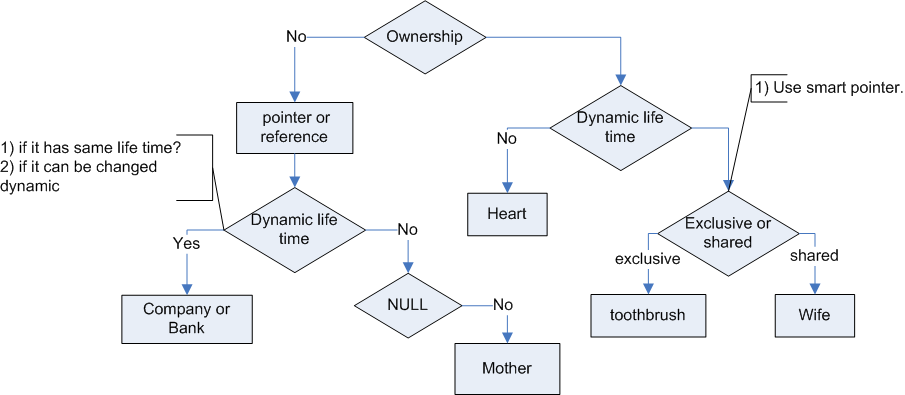
\includegraphics[width=0.92\linewidth]{pics/owner.png}
\end{center}


\begin{description}
	\item[Company or Bank] No ownership. Company is a member, It's important for you to have a work and it used by many member functions. so it's a member. For Bank,you just use it when you want to get Money, so use it in the function as parameter. Company is associate relationship and Bank is dependency relationship.
	
	\item[Monther] No ownership. It can not be null, and can not be changed.  so we use reference. 
	
	\item[Heart] Ownership, same life time, (No dynamic life)
	
	\item [Toothbrush] Ownership, dynamic life, and exclusive ownership, so we use \texttt{unique\_ptr}.
	
	\item [Wife] Ownership, dynamic life, and shared ownership, so we use \texttt{shared\_ptr}.
\end{description}


\end{itemize}

\subsection{Examples about classes relationship}
\begin{itemize}
	\item OOP example 1: If it's a car-engine (composition) relationship, and it's compiler-given(not dynamic), just use \textbf{member obj.}   Pay attention, If engine has no default constructor, you have to use initialization list in car constructor. 
\begin{lstlisting}[frame=single, language=c++]
class Car{
	Engine eng; // member obj, not use pointer here.
	Car(int carArg, int engArg): eng(engArg){}
}
	\end{lstlisting}
		
	\item OOP example 2:  If it's an peole-brush (Association) relationship, if it has same life time and exclusive ownership, use \texttt{uniqu\_ptr}. If you want to change, use \texttt{uniqu\_ptr} reset function or move semantic from another \texttt{uniqu\_ptr}.
\begin{lstlisting}[frame=single, language=c++]
class Person{
	unique_ptr<Brush> unpbrush;
	
	buyNewBrush(string &name){
		unpbrush.reset(new Brush());
	}
};
\end{lstlisting}
\begin{description}
	\item[Line 5:] you can't use \texttt{unpbrush= new Brush()}, \texttt{unpbrush} assignment only support( unique\_ptr< T > \&\&); use reset, it will make original deleted automatically. don't need destructor in Person class any more.
\end{description}
	
	\item OOP example 3: If it's wife-husband(Association) relationship, If you want to express \textbf{Strong Not Nullity}, use reference, such as Mother-Son association, You need to use initialization list to initialize mother. If Nullity, such as wife, just use raw pointer, \texttt{weak\_ptr} or \texttt{shared\_ptr}. Because no ownership involved, don't use uniqu\_ptr at all. 
	
	\item OOP example 3-1: What's different with raw pointer, weak\_ptr or shared\_ptr?
	\begin{lstlisting}[]
class Man{
	Woman*  wife; //Can be set to nullptr. maybe change or live longer than you.
	Woman& mother;  //Must initialize mother in initial list
}
\end{lstlisting}

	
	\item OOP example 4: If it's dependency,  such as friend relationship,  Most of time, we just use pointer or reference as function parameter.
\begin{lstlisting}[]
class Man{
	lendMoney(const Friend* mike);
	lendMoney(const unique_ptr<Friend>& mike);
	lendMoney(const shared_ptr<Friend>& mike);
}
\end{lstlisting}
\begin{description}
	\item[Line 2-4:] Just use it in function, not a member of class. Use const if don't want to change it.
\end{description}
	
	\item OOP example 5: Suppose Man and Computer(Associate from structure semantic) is has-a relationship and same life time. Don't use pointer or reference, just copy from a common computer, and maybe later you can customize your computer, and it will not effect common one.  We can copy from \texttt{commonComputer} and initialize all Worker object.  And this time use initialization list can improve efficiency.
\begin{lstlisting}[numbers=none]
class Worker{
	Computer m_desktop;
	Worker (Computer u): m_desktop(u){}
}
	
Computer commonComputer;
Worker Yan(commonComputer);
Worker Han(commonComputer);
\end{lstlisting}
	
	
	\item OOP example 6:  Change a semantic,  school may have a Bus, but \textbf{owner policy} tell us that bus can be shared by different schools. and \textbf{life time policy} tell us that bus and school has separate life time. so here, we should use \texttt{shared\_ptr}.
\begin{lstlisting}[numbers=none]
class School{
	shared_ptr<Bus> shr_p_bus;
}
\end{lstlisting}
	
	\item OOP example 7: Some classes provide a container to hold multiple objects of another type. A value container is a composition that stores copies of the objects it is holding. A reference container is an aggregation that stores pointers or references to objects that live outside the container. For example, \texttt{std::vector} and \texttt{std::map} are containers that can hold multiple objects of another type.
	
\end{itemize}


\section{Class design}

\subsection{Three big principles}
\begin{itemize}
	\item There are three basic rules about design pattern. One of them is Interface Segregation Principle(ISP), that is to say \textbf{Make Inferface simple and small.} The other two principles are:
\begin{enumerate}
	\item Liskov Substitution Principle(LSP)----Clients (Functions and Class) that use pointers or references to base classes must be able to use objects of derived classes without knowing it.  So all overrides of virtual member functions must \textbf{require less and provide more}. So you are able to make substitution successfully.
	
	\item Dependence Inversion Principle(DIP). client doesn't depend on implementation. \textbf{Both clients and implementation depend on interface.} The "inversion" in Dependency Inversion Principle refers to the reversal of this traditional dependency relationship, which is an inversion of the control of dependencies. Instead of high-level modules controlling and depending on low-level modules, the control is inverted so that low-level modules depend on high-level modules through abstractions. This inversion can result in a more flexible and maintainable system.
	\begin{figure}[h]
		\centering
		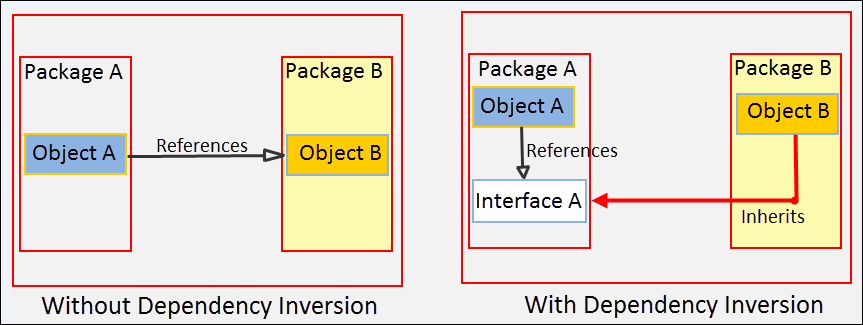
\includegraphics[width=0.66\linewidth]{pics/DIP.png}
		\label{fig:dip}
	\end{figure}
	
\end{enumerate}

	\item Example code below.  1)LSP: \texttt{Car} can use  \texttt{GasPower} or \texttt{ElePower} without know it. 2)DIP: \texttt{Car} only is depends on \texttt{Power*} interface 3)ISP: Interface should be small and separately. An example can be seen in MI section below.

\begin{lstlisting}
class Car{
	....................
	Power* pow //Pointer or reference to the base class (Power* pow)
};
Car::start(){
	...........
	pow->ignite(); //Virtual function support dynamic-binding
}
class Power{
	virtual ignite();
};

class GasPower : public Power
class ElePower : public Power
Car car(gas);
car.start();
\end{lstlisting}

\end{itemize}


\subsection{non-leaf classes abstract and NVI}

\begin{itemize}

	\item Inheritance has three usages: 1) I want to inherit a interface. (pure virtual, you have to rewrite ) 2) I want to inherit a implement, but I may want to change it. (virtual, you may or may not rewrite) 3) I want to inherit a implementation, but I don't want to change it. (Non-virtual, you can't rewrite it at all)
\begin{lstlisting}[numbers=none]
class shape{
public:
	virtual draw() = 0 // you have to re-implement.
	virtual error(); // there is default implement, but you may change it.
	int objectID(); // you should not rewrite it.
}	
\end{lstlisting}

	\item A problem with inheriting from a concrete type is that it creates some ambiguity as to whether code which specifies a certain type really wants an object of the specific concrete type, or wants an object of a type which behaves in the fashion that the concrete type behaves. This distinction is vital in C++, since there are many cases where operations which will work correctly on objects of a certain type will fail badly on objects of derived types. The problem can be illustrated by the assignment of pointer to base class. The problem has been introduced in "More effective C++ item 33"
	

	\item "non-leaf classes abstract" rule can be found in More effective 33 "making non-leaf classes abstract" and C++ coding standards 36 "Prefer providing abstract interfaces." They all said that you should only inherit from an abstract interfaces. It also follow DIP. When you found abstract conception appear in more than one context, you need build abstract interface for it. 


	\item NVI is making virtual functions nonpublic, and public function nonvirtual. This is similar with Template Method design pattern. About NVI, more detail can be found in "C++ coding standards Item 39" and "Virtuality herb sutter"

\begin{enumerate}
	\item Prefer to make interfaces nonvirtual, using Template Method.
	
	\item Prefer to make virtual functions private.
	
	\item Only if derived classes need to invoke the base implementation of a virtual function, make the virtual function protected. For the special case of the destructor only:
	
	\item A base class destructor should be either public and virtual, or protected and nonvirtual.
\end{enumerate}

    \item Below figure illustrates "Non leaf abstract", "DIP", "NVI" and template method. You should learn this example and do you best to understand all ideas behinds it. 

	\centering
	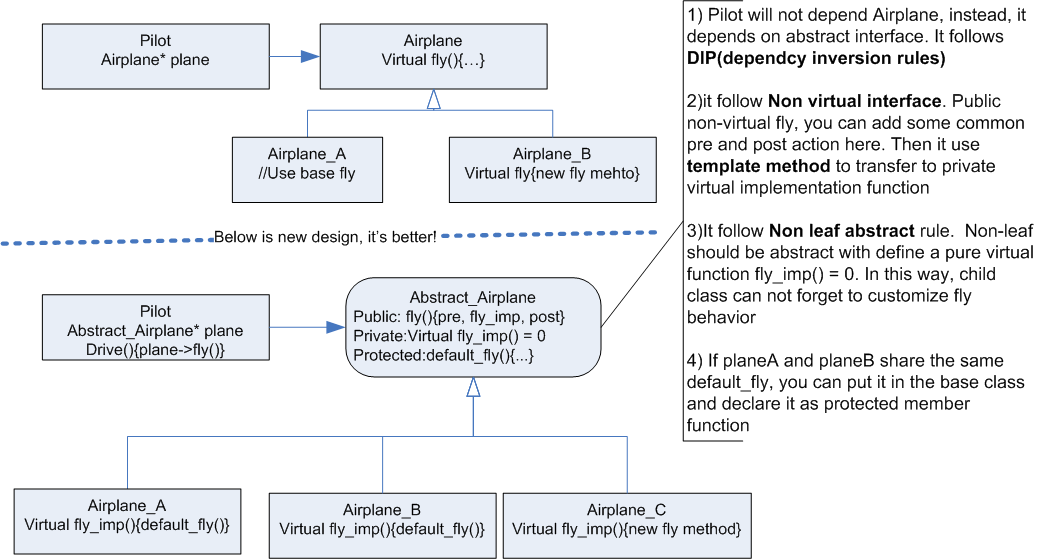
\includegraphics[width=0.93\linewidth]{pics/NVI.png}

\end{itemize}

\subsection{Common used design pattern}
\begin{itemize}
	
		\item Observer pattern: A way of notifying change to a number of classes. Define a one-to-many dependency between objects so that when one object changes state, all its dependents are notified and updated automatically.
	
	\begin{center}
		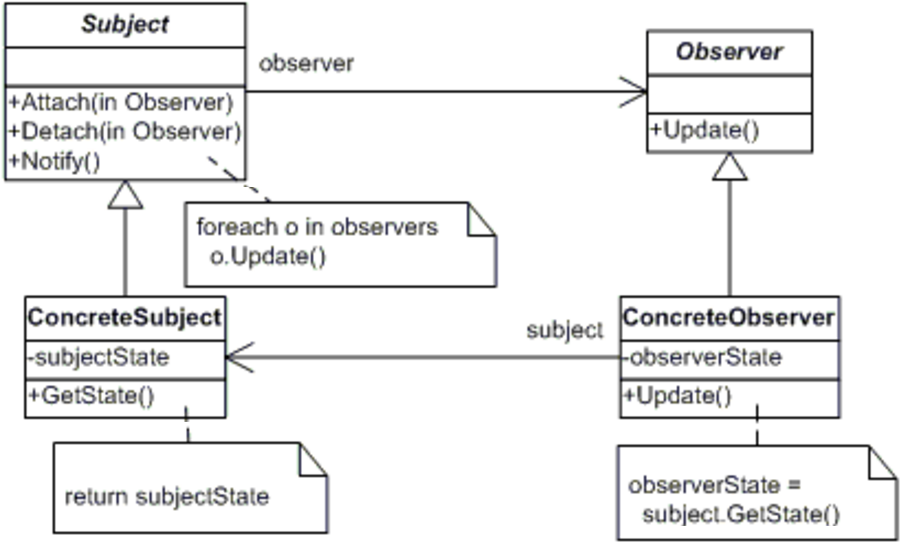
\includegraphics[scale=0.5]{pics/observer.png}
	\end{center}
	
	
	\item Observer includes update(); Subject includes addObserve(), deleteObserve(), notify(). 
	
	\item Composite pattern: A tree structure of simple and composite objects. Compose objects into tree structures to represent part-whole hierarchies. Composite lets clients treat individual objects and compositions of objects uniformly.

\begin{figure*}
	\centering
	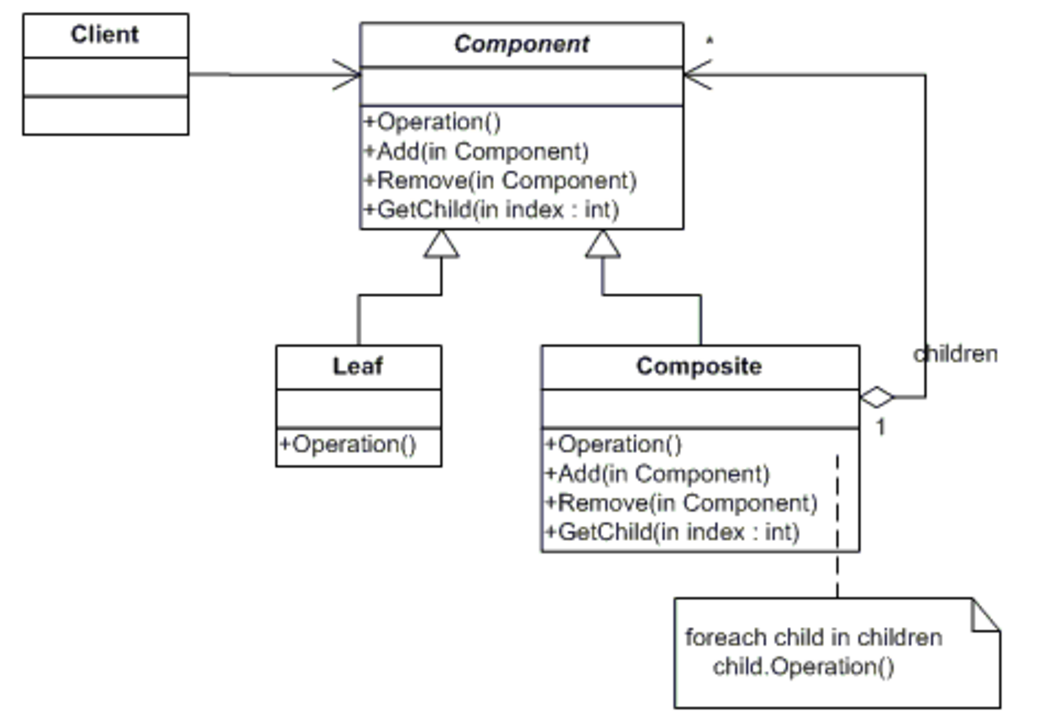
\includegraphics[width=0.49\linewidth]{pics/composite.png}
	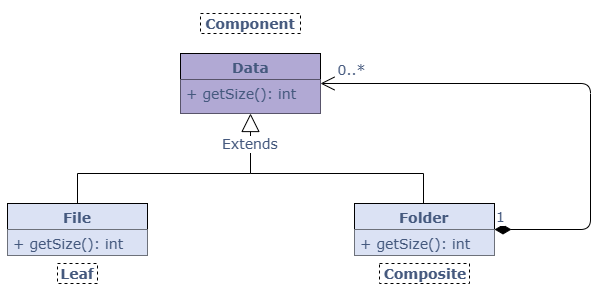
\includegraphics[width=0.49\linewidth]{pics/com_file.png}
\end{figure*}


		
	\item It can be use as recursive Tree structure. Such as file tree. A folder is composite, and a file is component, and a folder can be a component of another composite. 
	
%\begin{center}
%	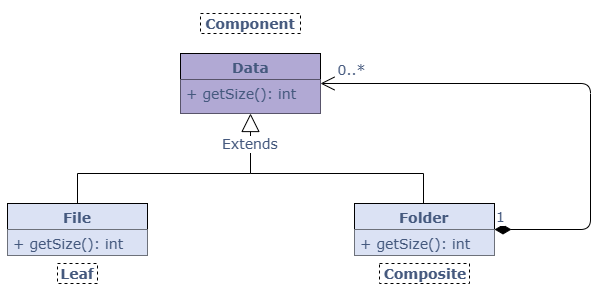
\includegraphics[scale=0.6]{pics/com_file.png}
%\end{center}
	
	
\end{itemize}

\subsubsection{MI or bridge}
\begin{itemize}
	
	\item "If a class has two superclasses that share a common base class, multiple inheritance can cause the diamond problem, where a subclass inherits two copies of the shared base class. To solve this problem, you can use the virtual keyword and follow the new constructor rules, which are described in detail in C++ Primer on page 815. It's important to carefully consider the use of multiple inheritance and only use it when necessary.
	
\begin{lstlisting}[numbers=none]
Father 1: virtual public grandfather
Father2: virtual public grandfather
son : public Father1, public Father2	
\end{lstlisting}	
	
	\item Suppose you have land vehicles, water vehicles, air vehicles, and space vehicles. (Forget the whole concept of amphibious vehicles for this example; pretend they don't exist for this illustration.) Suppose we also have different power sources: gas powered, wind powered, nuclear powered, pedal powered, etc. We could use multiple inheritance to tie everything together, but before we do, we should ask a few tough questions:
	
	\begin{enumerate}
		\item Will the users of Land Vehicle need to have a Vehicle\& that refers to a LandVehicle object? In particular, will the users call methods on a Vehicle-reference and expect the actual implementation of those methods to be specific to LandVehicles?
		
		\item Ditto for GasPoweredVehicles: will the users want a Vehicle reference that refers to a GasPoweredVehicle object, and in particular will they want to call methods on that Vehicle reference and expect the implementations to get overridden by GasPoweredVehicle?
	\end{enumerate}
	If both answers are "yes," multiple inheritance is probably the best way to go.
\begin{lstlisting}[numbers=none]
Class GasPowered :public Power //method 1: Multiple inheritance
Class LandVehicle :public Vehicle
Class LandVehicleGasPowered :public GasPowered, LandVehicle 

Class Vehicle{   //method 2: Bridge design pattern
	//
	Power * _power;
}

Class LandVehicle :public Vehicle  // method 3: Nested generalization.
Class LandVehicleGasPowered: public LandVehicle
\end{lstlisting}
	
	\item There are at least three choices for the overall design: the bridge pattern, nested generalization, and multiple inheritance. Each has its pros/cons:
	\begin{center}
		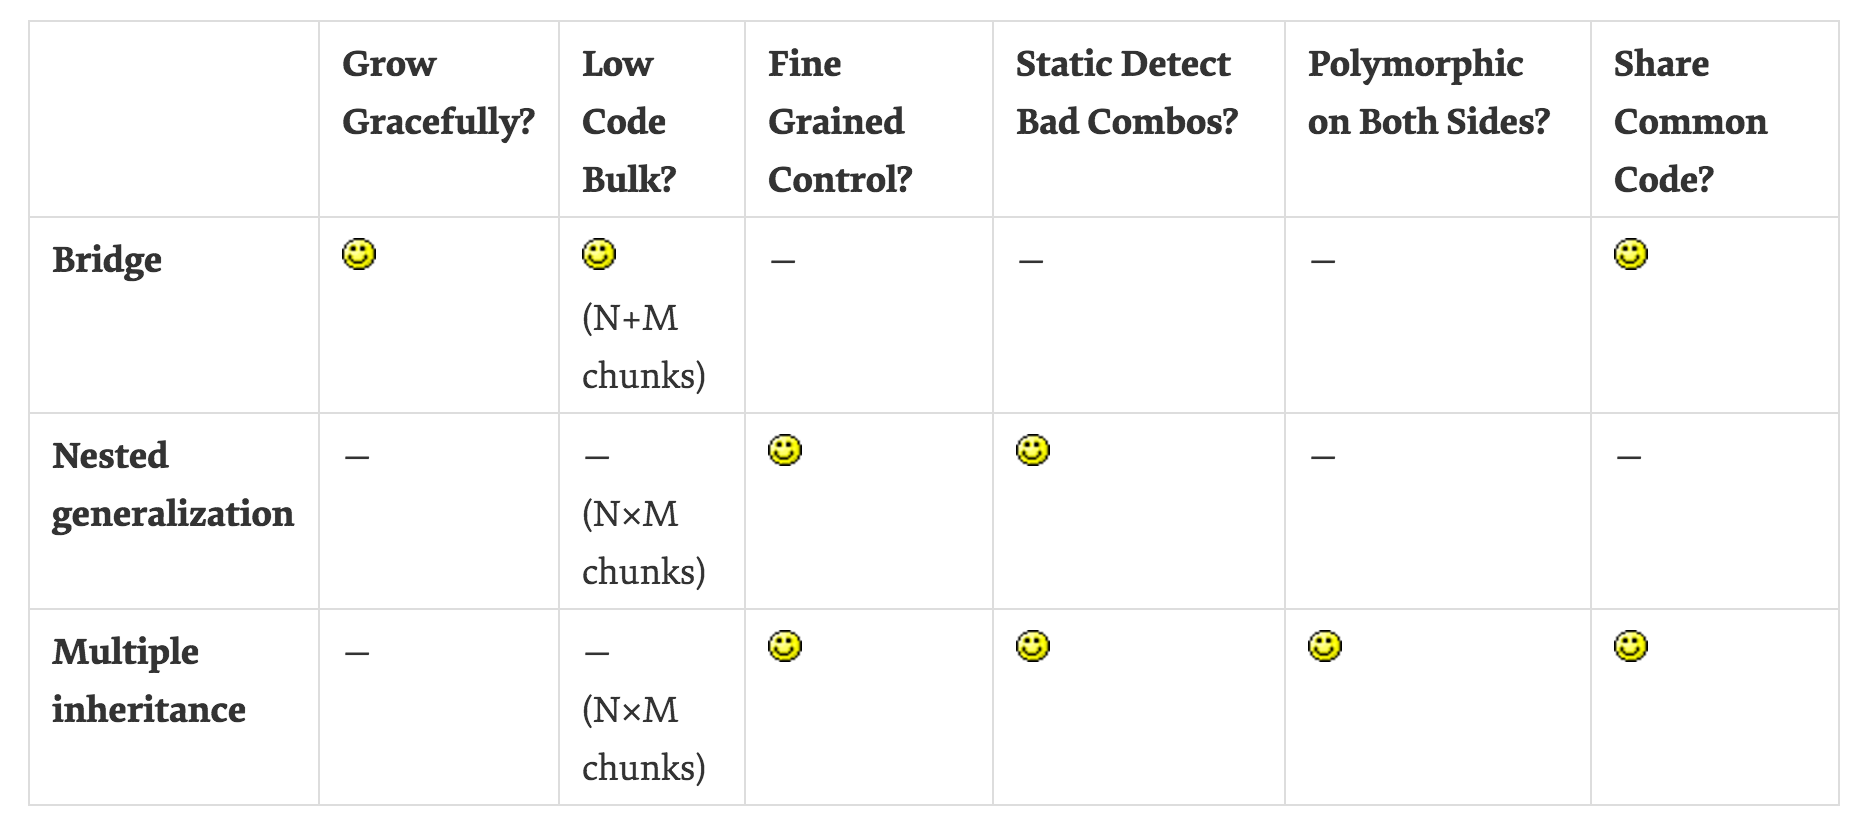
\includegraphics[scale=0.38]{pics/MI.png}
	\end{center}
	
	
	\item Try especially hard to use ABCs when you use MI. In particular, most classes above the join class (and often the join class itself) should be ABCs. In this context, "ABC" doesn't simply mean "a class with at least one pure virtual function;" it actually means a pure ABC, meaning a class with as little data as possible (often none), and with most (often all) its methods being pure virtual.
	
	\item A design discussion can be seen in "C++ FAQ Inheritance-- Multiple and Virtual Inheritance"
	
\end{itemize}


\subsubsection{factory method, strategy and template method}
\begin{itemize}
	\item These three patterns have the similar UML structure, but different applications context.
	
\begin{center}
	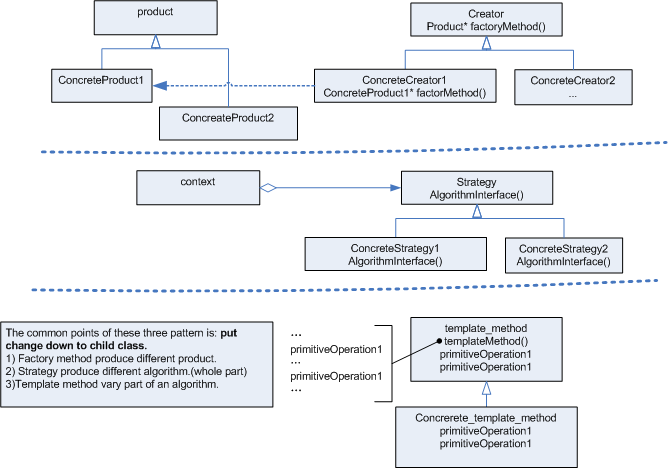
\includegraphics[width=0.93\linewidth]{pics/template_method.png}
\end{center}

	\item Comparison between these three patterns. The common points is push the change down into the child class. In factory method, we push the generating algorithm down to the child class. In strategy, we push the whole algorithm. In template method, we push the part of algorithm down to the child class. That idea has been used widely in the famous 23 design pattern. 
	 
\end{itemize}


\subsubsection{Comparsion between factory, bridge and visitor}

\begin{itemize}
	\item Factory, bridge and visitor, these three design patterns share the same UML structure, so I will introduce them together. One is a creational pattern, one is a structural pattern, and the last one is a behavioral pattern. However, it's important to note that design patterns are based on \textbf{semantics} and concrete applications, not on \textbf{UML relationships and structures}.
	
	\item This is an example that uses the abstract factory, bridge, and visitor design patterns with bicycles and cars. Both bicycles and cars can use either a gas engine or an electric engine, resulting in four different vehicles: gas bicycle, gas car, electric bicycle, and electric car. This is the context of our example.

	\item The figure below illustrates the basic ideas and implementations of the three patterns. Each pattern consists of two basic abstract concepts and their relationships, such as (Factory--create--Engine), (Vehicle--implement--Engine), and (Vehicle--visit--Visitor). When using double dispatch, it's important to understand the broader meaning of "visit". 	
	
	\item visit pattern also support double dispatch, how to understand it? From semantic point of view, vehicle type and refillor type (two types) decide Refill method . From source code point of view, \texttt{Vehicle} first decide a \texttt{Refillor} (\texttt{Electric} or \texttt{Oil}), once it decide one(for example \texttt{Electric}), then pass \texttt{this} pointer to decide \texttt{Refill(Car*)} or \texttt{Refill(Bicyle*)} inside of ElectricRefill class. That is double dispatch, element(Vehicle) accept visitor(Refillor) base class pointer, and pass \texttt{this} pointer to visitor's visit method(Refill). 
	
\begin{center}
			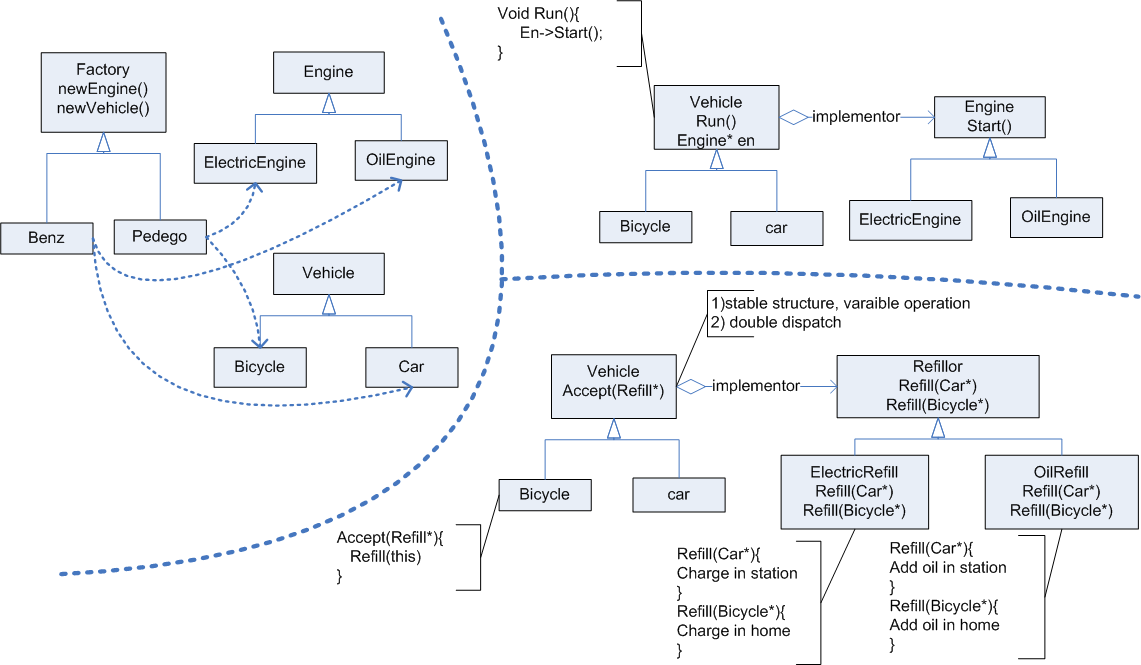
\includegraphics[width=0.95\linewidth]{pics/visitor.png}
\end{center}

	    
\end{itemize}

\chapter{Exception and error}
\section{debug}
\begin{itemize}
	\item A few useful debugger commands in linux
	\begin{enumerate}
		\item cgbd: terminal-based frontend for gdb, sudo apt-get install cgbd (sudo apt install -y cgdb)
		\item gdbgui: brower-based frontend for gdb, https://gdbgui.com,  sudo pip install gdbgui
		\item visual studio code: can connect to gdb. 
	\end{enumerate}
	
	\item Usually compiler command switch and tool
\begin{lstlisting}
g++ a.cpp -o a -fsanitize=address
g++ a.cpp -o a -fsanitize=undefined

valgrind [options] ./a [program options]
valgrind --tool=memcheck ./a
valgrind --tool=callgrind ./a // runtime profiling
valgrind --tool=drd ./a // multithreading error detection	
\end{lstlisting}	
	
	\item Recommended compiler flags for your first programs.
\begin{lstlisting}
g++ -std=c++20 -Wall -Wextra -Wpedantic -Wshadow -Werror input.cpp -o output	

// below is production level recommended set
-Wall -Wextra -Wpedantic -Wshadow -Wconversion -Werror -fsanitize=undefined,address -Wfloat-equal -Wformat-nonliteral -Wformat-security -Wformat-y2k -Wformat=2 -Wimport -Winvalid-pch -Wlogical-op -Wmissing-declarations -Wmissing-field-initializers -Wmissing-format-attribute -Wmissing-include-dirs -Wmissing-noreturn -Wnested-externs -Wpacked -Wpointer-arith -Wredundant-decls -Wstack-protector -Wstrict-null-sentinel -Wswitch-enum -Wundef -Wwrite-strings	
\end{lstlisting}	
	
	
\end{itemize}

\section{Terminate application}
%\subsection{Different methods to terminate}
\begin{itemize}
	\item In the C language, you can call \texttt{abort()}, \texttt{exit()}, \texttt{quick\_exit()}, and \texttt{\_exit()} to end your program at any time. They are all declared in the \texttt{<cstdlib>} header file.
	
	\item \texttt{exit( status )} terminates the process normally. A status value of 0 or EXIT\_SUCCESS indicates success, and any other value or the constant EXIT\_FAILURE is used to indicate an error. \texttt{exit()} performs the following operations: 1) flushes any unwritten buffered data, 2) closes all open files, and 3) may remove any temporary files that were created by the program (depending on how they are managed). When you call exit or execute a return statement from main, static objects are destroyed in the reverse order of their initialization.
	
	\item \texttt{atexit()} registers the function pointed to by func to be called on normal program termination (via \texttt{std::exit()} or returning from the main function)
\begin{lstlisting}[]
void myProgramIsTerminating1(void){
	cout<<"exit main function"<<endl;
}

int main(int argc, char**argv){
	atexit (myProgramIsTerminating1);
	//abort(); abort will not call myProgramIsTerm
}	
\end{lstlisting}		
	
	\item C++11 introduced \texttt{quick\_exit()}, which was added specifically to deal with the difficulties of ending a program cleanly when using threads. \texttt{std::quick\_exit()} is similar to \texttt{\_exit()}, but with the added option to execute some code that was registered with \texttt{at\_quick\_exit} before the program terminates."
	
	\item \texttt{\_exit()} is called without performing any of the regular cleanup tasks for terminating processes, while \texttt{abort()} is called without destroying any objects and without calling any of the functions passed to \texttt{atexit} or \texttt{at\_quick\_exit}. However, if core dumps are enabled, \texttt{abort()} will dump the core. You can use this core dump to debug your program by analyzing it. Here's how to generate and use a core dump: when your program has an invalid memory operation, running the program may result in the following message:
\begin{lstlisting}[]
*** stack smashing detected ***: terminated
Aborted (core dumped)
\end{lstlisting}
	
	If you want your application to generate core dump, you need to run below commands:(In Ubuntu system)
\begin{lstlisting}[]
ulimit -c unlimited //configure once core file size limited,
sudo service apport start //run once to start apport.
./a.out //this will cause core dump
cat /var/log/apport.log // to see if core dump has been generated. 
gdb a.out /var/lib/apport/coredump/core.youname  // how to use core dump file
bt // give bt command in gdb enviroment, then you will know where 
// your programme perform invalid memory operation.	
\end{lstlisting}	
	
	\item When you use gdb, abort can list stack frame information for you. It's very helpful for you to debug.  Exit just end the application. When you use gdb, it shows nothing.
	
	\item When \texttt{assert} fail, it just calls \texttt{abort}. 
\begin{lstlisting}[numbers=none]
assert(! "You should not reach here");
\end{lstlisting}
	
	\item \texttt{std::terminate()} will be automatically called in a C++ program when there is an unhandled C++ exception. This is essentially the C++ equivalent of \texttt{abort()}. \texttt{std::terminate()} calls a handler that is set by the \texttt{std::set\_terminate()} function, which by default simply calls \texttt{abort()}.
	
	\item Don't use \texttt{exit()} in \texttt{main()}. It will not destroy local objects in the \texttt{main()} function. Instead, catch the exceptions that you can't handle in \texttt{main()} and simply return from there. This guarantees that stack unwinding happens correctly and all destructors are called.
\begin{lstlisting}[numbers=none]
int main() {
	try {
		// your stuff
	}
	catch( ... ) { // catch all exceptions.
		return EXIT_FAILURE;
	}
}	
\end{lstlisting}	
	
	\item In C, issuing a return statement from the \texttt{main} function is equivalent to calling the \texttt{exit} function with the return value as its argument. However, in C++, there are some subtle differences. When you call return in \texttt{main()}, destructors will be called for locally scoped objects. If you call \texttt{exit()}, no destructor will be called for locally scoped objects. Therefore, it's best not to use \texttt{exit} in C++. Instead, use try and catch(...) and then return EXIT\_FAILURE to ensure that the stack has been successfully unwound. \texttt{exit} is a C function and is not aware of, nor compatible with, C++ idioms. It does not perform cleanup on your objects, including those in the same scope. This means that your file may not be closed properly, and as a result, the content might never get written into it!
	
	
	\item The difference between \texttt{exit} and \texttt{abort} is that \texttt{exit} allows the C++ run-time termination processing to take place (global object destructors get called), but \texttt{abort} terminates the program immediately. The \texttt{abort} function bypasses the normal destruction process for initialized global static objects. It also bypasses any special processing that was specified using the \texttt{atexit} function. That is to say, if you use \texttt{abort()}, no objects will be destroyed. That is, no global objects, no static objects and no local objects will have their destructors called.
	
	\item According to previous introduction, if you want to end application in the other fun, you need to throw a exception, then leave it un-handle or re-throw it until it reaches \texttt{main}. In this way, stack unwinding will make sure all the destructor will be called.
\begin{lstlisting}[frame=single, language=c++]
try{
	fun(){
		throw end_exception();
	}
}
catch(end_exception& ex){
	//do something here
	throw;
}		
\end{lstlisting}		
	\begin{description}
		\item[Source code:] Just skip the entire catch block. When the exception reaches the end of the catch block or is not caught at all, it will propagate to the \texttt{main} function where all local objects will be cleaned up properly. When \texttt{main} returns, it will perform the necessary flush operations and destruct all local objects.
	\end{description}
	
\end{itemize}


%\section{Bug and assert}
%\subsection{Use assert}
%
%\begin{itemize}
%	
%%	\item You can implement trace by you self.
%%\begin{lstlisting}[numbers=none]
%%#if defined NDEBUG
%%	#define TRACE( format, ... )
%%#else
%%	#define TRACE( format, ... )   printf( "%s::%s(%d)"
%%	format, __FILE__, __FUNCTION__,  __LINE__, __VA_ARGS__ )
%%#endif
%%	\end{lstlisting}
%	
%\end{itemize}

\section{Handling exceptions}



\subsection{Handle error in C}
\begin{itemize}

\item There are three common error handling methods: 1) a global error code (C) or error state (C++), 2) return value, and 3) exception.
\begin{lstlisting}[frame=single, language=c++]
errno(), strerror()  //C language
cin.fail()  //C++ language
\end{lstlisting}

\item Besides above, you can use some custom function pointer to do some customized error handling behavior, such as \texttt{set\_new\_handler} function for new operator

\item \texttt{errno()} and \texttt{strerror()} is a typical C language style.

\begin{enumerate}
	\item In general, you should detect errors by checking return values, and use \texttt{errno} or \texttt{perror()} only to distinguish among the various causes of an error, such as "File not found" or "Permission denied."
	
\begin{lstlisting}[numbers=none]
FILE * pFile = fopen ("unexist.ent","rb");
if (pFile==NULL)
perror ("The following error occurred");
\end{lstlisting}
	
	\item It's only necessary to detect errors with \texttt{errno} when a function does not have a unique, unambiguous, out-of-band error return (that is, because all of its possible return values are valid; one example is \texttt{atoi()}). 
	%		In these cases (and in these cases only; check the documentation to be sure whether a function allows this),
\begin{lstlisting}[numbers=none]
#include <cerrno>
errno = 0  // set it zero before call any math library function.
double not_a_number = std::log(-1.0);
if (errno == EDOM) 
std::cout << "log(-1) failed: " <<std::strerror(errno) << '\n';	
\end{lstlisting}	
	\item You can detect errors by setting \texttt{errno} to 0, calling the function, and then testing \texttt{errno}. Setting \texttt{errno} to 0 first is important, as no library function ever does that for you.
\end{enumerate}

\item C11 provide \texttt{fenv.h} file to expand \texttt{errno}
\begin{lstlisting}[frame=single, language=c++]
#include <math.h>       /* math_errhandling */
#include <errno.h>      /* errno, EDOM */
#include <fenv.h>
/* feclearexcept, fetestexcept, FE_ALL_EXCEPT, FE_INVALID */

#pragma STDC FENV_ACCESS on
errno = 0;
if (math_errhandling & MATH_ERREXCEPT)
feclearexcept(FE_ALL_EXCEPT);

sqrt (-1);
if (math_errhandling & MATH_ERRNO) {
	if (errno==EDOM) 
	printf("errno set to EDOM\n");
}	
if (math_errhandling  &MATH_ERREXCEPT) {
	if (fetestexcept(FE_INVALID)) 
	printf("FE_INVALID raised\n");
}	
\end{lstlisting}

\end{itemize}

\subsection{Exceptions or Bug?}
\begin{itemize}

\item \textbf{Is it a bug or exception?} Exceptions are typically events that are beyond the control of the program or the user, while bugs are problems that are within the control of the program and can be fixed by changing the code. In other words, exceptions are things that can happen even if the program is perfectly correct, while bugs are things that should never happen if the program is written correctly. A practical example of an exception is a dead battery in a cell phone, but having diarrhea is an abnormality and not an exception. For example, a failure to open a file is an exception and you should throw an exception for it. On the other hand, if \texttt{age<0}, it is an abnormality which is shouting out: "I am a bug, fix me now!".
\begin{lstlisting}[numbers=none]
FILE *f = fopen("hr.dat".....);
if(f==nullptr){   //it's exception, don't use assert here.
	return -1;
	throw runtime_error();
}
	
assert(age>=0); //Here use assert, because age<0 is bug, not exception.
fprintf(f, %d, age);	
\end{lstlisting}


\item You can also think of an exception as a runtime error and a bug as a logical error. For logical errors, you need to rewrite the code to fix them. For runtime errors, you need to throw and catch exceptions to handle them. Logical errors should be identified as soon as possible using assertions or unit tests. Distinguishing between these two different conditions is important and it does not depend on the phenomenon but rather on the cause. For example, in the function \texttt{f(Foo* p)}, if \texttt{p} is \texttt{nullptr}, there are two possibilities reasons:

\begin{enumerate}
	\item They may be passing \texttt{nullptr} because they received bad data from an external user (for example, the user forgot to fill in a field and the database connection failed). In this case, you should throw an exception since it is a runtime situation (i.e., something that cannot be detected by a careful code-review; it is not a bug). 
	
	\item \texttt{nullptr} is caused by a mistake in their own code. you should definitely fix the bug in the caller's code. but you must not merely change the code within \texttt{f(Foo* p);} you must, Must, MUST fix the code in the caller(s) of \texttt{f(Foo* p)}.
\end{enumerate}

\item In previous example, You can use assert first, after you code-review, found that It's not bug, but cause by an exception, such as net disconnect. so you can change assert to throw. THAT IS  A GOOD STRATEGY!

\begin{lstlisting}[frame=single, language=c++]
fun(int* pi, int j){
	assert(j< 10); //logic error, You can assert it 
	assert(pi == nullptr)
	
	if(file.open()) //runtime error
	throw runtime_error();
}		
\end{lstlisting}

\item assert is a preprocessor macro (more about them later) and commas would otherwise be interpreted as macro argument separator:
\begin{lstlisting}
assert( min(1,2) == 1 );  //  ERROR
assert( (min(1,2) == 1) );  //  OK	
\end{lstlisting}

\item Assertions are deactivated by defining preprocessor macro NDEBUG, e.g., with compiler switch: \texttt{g++ -DNDEBUG …}

\item Bugs should be found as early as possible. There are two basic methods to achieve this: using assertions and conducting unit tests. I will introduce unit testing in the 'Testing' chapter.

\item The idea behind using \texttt{assert} is to immediately spot an abnormal case that may otherwise cause errors in other parts of the code. Without an \texttt{assert}, it may be difficult to trace the error back to its source position.
\begin{lstlisting}[frame=single, language=c++]
fun(char* p){
	assert(p!=nullptr);
	...... // a lot of codes here
	strcpy(p)  //error happen here
	fun1(p);  //or it will cause error in other place.
}		
\end{lstlisting}

\item You can use \&\& to make assert print out more useful information. string literal is always true; when \texttt{I<5} is false, the whole condition will be printed out.
\begin{lstlisting}[frame=single, language=c++]
#include <cassert>
assert(I<5 && "I is more than 5");	
\end{lstlisting}

\item Assert is just \texttt{if()}+\texttt{abort()}: Difference of assert and return error(throw exception) is that abort will terminate you application immediately, and you can use GDB to trace back source easily.

\item the usage of assert depends on the context, but it's not always recommended to use assert to its fullest. Precondition and postcondition assertions are two important types of assertions, but there are other types of assertions that can also be useful, such as invariants, boundary checks, and null checks. Precondition assertions are used to test the validity of the arguments passed to a method before the method is executed. Postcondition assertions are used to test the validity of the results produced by the method after the method has completed its execution.

\end{itemize}

\subsection{Exceptions in C++}
\begin{itemize}
\item If you don't know if you should use exception, then you should use it in your project. In other word, if you don't have any solid reason to against it, just use it.

\item Exceptions mainly handle runtime errors. They are potentially recoverable errors, such as attempting to open an unavailable file or requesting more memory than is available.
\begin{enumerate}
	\item A file write operation failed or file access operation failed because this file doesn't exist.
	
	\item No enough memory.
	
	\item invalid value, which come from user input, not come from you error code logic.
	
	\item System communication software invalid protocol, format, or no response.
\end{enumerate}

\item unwinding the stack has cost problems, it make program 10\% larger and slower. So you can use \texttt{-fno-exceptions} to stop it.

\item Exception specification is add \texttt{throw} keyword in the end of function, no throw means that it will throw any exceptions, and \texttt{throw()} means it will not throw any exceptions. Throw( e1, e1) means that it will throw two kinds of exceptions. In C++, this feature has been unsupported and only one left is use throw() to indicates that it will not throw any exceptions. In modern C++, we use \texttt{noexcept} to replace throw(). Pay attention here: exception specification doesn't use very well with template. construct, destruct and assignment will become \texttt{noexcept} if the functions they are calling are noexcept. 

\item A simple exception can be a char string, then using \texttt{const char* c} to catch it. A more complicate example is exception class, and you can define the exception class, and throw \texttt{exception\_class}, than use \texttt{exception\_class \& }ec to catch it.  

\item You don't need explicit define \texttt{exception\_class} object and throw this object; throw \\ \texttt{exception\_class()}; will avoid copy and is recommend way to follow.
\begin{lstlisting}[numbers=none]
throw exception_class{}; //good style

exception_class ex; //bad style.
throw ex	
\end{lstlisting}


\item You can build an exception class inside the C++ standard exception system. It needs to derive your class from exception and redefine the function what(). If your exception class has a very tight relationship with your real class, it can be declared as a nested class.

\begin{lstlisting}[numbers=none]
Class my_ex :public std::exception{
	const char* what(){return "my_ex reason is here"}
}	
\end{lstlisting}


\item Standard exception includes \textbf{logic\_error, domain\_error,  runtime\_error.  Invalid\_argument, out\_of\_bounds, range\_error, overflow\_error.}

\begin{center}
	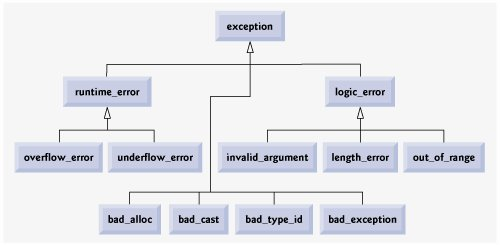
\includegraphics[scale=0.8]{pics/exception.jpg}
\end{center}



\item Common pattern of try catch block:
\begin{enumerate}
	\item Handle an exception and continue executing, place the code in separate try-catch blocks. 
	
\begin{lstlisting}[frame=single, language=c++]
try{ 
	// code that throws an exception	
}
catch (Exception1& ex){
	// handle
}

try{ 
	// this code will execute unless the previous catch block 
	// throws an exception (re-throw or new exception) 
}
catch (Exception2 ex){
	// handle
}			
\end{lstlisting}
	
	\item When exception happen, we have to deal with immediately and don't want to continue to run, can use one try and multi catch blocks. 
\begin{lstlisting}[frame=single, language=c++]
try{ 
	// code that throws an exception	
	// this line won't be executed. 
}
catch (Exception1& ex){
	// handle
}
catch (Exception2 ex){
	// handle
}				
\end{lstlisting}		
	
	
	\item Properly order your catch-clauses. Arranging the catch blocks in inverse order of derivation. Catch by using reference: 1) It will support polymorphic exception, and catch exception from specific to generic. 2) It will avoid extra copying.
\begin{lstlisting}[frame=single, language=c++]
void f(){
	// ...
	try {
		// ...
	}
	catch (Base& b) { /* ... */ }  //The order is WRONG here!
	catch (Derived& d) { /* ... */ } //base shadows Derived
	catch (...) { /* ... */ }        //... shadows std::exception&
	catch (std::exception& e) { /* ... */ }
}	
\end{lstlisting}	
	
	\item Empty throw means that you throw present exception again.
\begin{lstlisting}[frame=single, language=c++]
catch(my_base_ex &ex){
	......
	throw; //not using throw ex, maybe ex is child class
}	
\end{lstlisting}		
	
	\item Don't use all throw and catch to replace return-code. For a simple function, if just return one error code and user will not forget to test return code, return-code method is more efficient than try catch. 
\end{enumerate}

\item Compared with return error code, exception has advantage:
\begin{enumerate}
	\item  Can catch deeper called function exceptions. If you want to use return value, deeper called function is hard to deal with.
	
	\item Difficult to return value: 
	\begin{enumerate}
		\item No return value, such as class constructor.
		\item All return value is normal value, such as \texttt{atoi()}.
	\end{enumerate}
	
	\item Make correct path and error-handle path separately and clearly.
	
	\item You can't ignore exceptions; any unhandled exception can result in termination of the program.
\end{enumerate}


\item \textbf{Never throw any exception in destructor.} In another word, Destructors and deallocation must never fail. In you destructor, don't throw any exception, or catch all the exception inside of it. Otherwise it will call \texttt{std::terminate} to stop the application. see more effective C++ exception chapter. However, throwing an exception in constructor is the best way to signal an error during object construction. Since there's no return value, there's no other way, other than constructing a headless object, which is bad style in C++.

\item In C++, the lifetime of an object begins when its constructor completes and ends when its destructor is called. If the constructor throws an exception, the destructor is not called for that object. However, the destructors of any member variables whose constructors have already completed are still called.

\end{itemize}

\section{Usage suggestions}
\begin{itemize}
\item All standard containers must also implement the strong guarantee for all operations (with two exceptions). They always have commit-or-rollback semantics so that an operation such as an insert either succeeds completely or else does not change the program state at all. "No change" also means that failed operations do not affect the validity of any iterators that happened to be already pointing into the container. There are only two exceptions to this point. First, for all containers, multi-element inserts ("iterator range" inserts) are never strongly exception-safe. Second, for vector<T> and deque<T> only, inserts and erases (whether singleor multi-element) are strongly exception-safe as long as T's copy constructor and assignment operator do not throw. Note the consequences of these particular limitations. Unfortunately, among other things, this means that inserting into and erasing from a vector<string> or a vector<vector<int> >, for example, are not strongly exception-safe.

\item Exception handling is highly dependent on your application context. So it should be designed into a program rather than just added on. Consciously specify, and conscientiously apply, what so many projects leave to adhoc (mis)judgment: Develop a practical, consistent, and rational error handling policy early in design, and then stick to it. Ensure that it includes:

\begin{enumerate}
	\item Identification: What conditions are errors.
	\item Severity: How important or urgent each error is.
	\item Detection: Which code is responsible for detecting the error.
	\item Propagation: What mechanisms are used to report and propagate error
	notifications in each module.
	\item Handling: What code is responsible for doing something about the error.
	\item Reporting: How the error will be logged or users notified.
\end{enumerate}


\item For different runtime errors, you can take various actions. And it's depends on you context of application.

\begin{enumerate}
	\item Error is just warning, log or show it to user, then continue;
	\item Error can be resolved inside a function, the whole application can be continue after you resolve or retry, such as input error.
	\item Set global error code or return error code or throw exception. then caller decide what to do (return a error code or use exception)
	\item Errors can be serious and prevent an application from continuing, in which case it should stop gracefully (by throwing an exception to main function and return from there), or request debugging (by calling abort).
\end{enumerate}

\item When to use assert ?
\begin{enumerate}
	\item Your problem comes from your own bad code, it's better to use ASSERTs.  Including you coding error or addition overflow.
	
	\item Bugs in your program are not something the user can handle, User can do nothing when he face "age should be not negative" unless age is inputted by himself(at this time, you should use return error code)
	
	\item You have to stop your application. If you write negative age back to database, It may cause futuristic error for other user later, and It's very difficult to trace back.
\end{enumerate}

\item When to throw a exception( or return error code)? Exception and return a error code has the same philosophy. \textbf{let caller decide what to do next}.

\begin{enumerate}
	\item As a general rule of thumb, throw an exception when your program can identify an \textbf{external problem} that prevents execution.
	
	\item Identify problems that the program can't handle and inform the user about them, because the user can handle them. For example, running out of memory space, non-existent file, no net connection, failed object construction, and receiving invalid data from the server, etc.
\end{enumerate}

\item When to use try... catch block? Catch an exception where you can do something useful with it.

\begin{enumerate}
	\item You can actually handle the exception. your catch clause deals with the error and continues execution without throwing any additional exceptions. My caller never knows that the exception occurred.
	
	\item I can have a catch clause that does blah blah blah, after that I will rethrow the exception. In this case, consider changing the try block into an object whose destructor does blah blah blah. For instance, if you have a try block whose catch clause closes a file then rethrows the exception, consider replacing the whole thing with a File object whose destructor closes the file. This is commonly called RAII
	
	\item Show some message or log exception, or give user a list options to select.  then rethrow.
\end{enumerate}

\item Exception in C++ is a tool; use it properly and it will help you; Don't blame the tool if you use it improperly. "Wrong exception-handling mindsets" in c++ FAQ website section 17 is good topic. You need to read it.

\end{itemize}


     
\chapter{Generic programming}
     
\section{Type deduction basic}


\subsection{template type deduction}
\begin{itemize}

	\item In the code provided below, we will explain the basic rules for type deduction.
\begin{lstlisting}[numbers=none]
template<typename T>
void f(ParamType param);

f(expr); // deduce T and ParamType from expr
\end{lstlisting}

\begin{enumerate}
	
	\item ParamType is a reference or pointer, but not a Universal Reference. If expr's type is a reference, \textbf{ignore the reference part}, then pattern-match expr's type against ParamType to determine T.
\begin{lstlisting}[frame=single, language=c++]
template<typename T>
void f(T& param); // param is a reference
	
int x = 27; // x is an int
const int cx = x; //cx is a const int
const int& rx = x; //rx is a reference to x as a const int
f(x);    //T is int param's type is int&
f(cx);   //T is const int, param's type is const int&
f(rx);   //T is const int, param's type is const int&
\end{lstlisting}
	
	\item If ParamType is a Universal Reference, we use different rule for lvalue and rvalue.
	
	\begin{enumerate}
		\item If expr is an lvalue, both T and ParamType are deduced to be lvalue references. Although ParamType is declared using the syntax for an rvalue reference, its deduced type is an lvalue reference.
		
		\item If expr is an rvalue, the "normal" (i.e., Case 1) rules apply.
	\end{enumerate}
	
\begin{lstlisting}[frame=single, language=c++]
template<typename T>
void f(T&& param); // param is now a universal reference
int x = 27; // as before
const int cx = x; // as before
const int& rx = x; // as before
	
f(x);   //x is lvalue, so T is int& param's type is also int&.
f(cx);  //cx is lvalue, so T  and param's type are const int&.
f(rx);  //rx is lvalue, so T  and param's type are const int&.
f(27);  //27 is rvalue, so T is int, param's is therefore int&&.
\end{lstlisting}

	
	\item ParamType is neither a pointer nor a reference. As before, if expr's type is a reference, ignore the reference part. If, after ignoring expr's reference-ness, expr is const, ignore const too. If it's volatile, also ignore that.
\begin{lstlisting}[frame=single, language=c++]
template<typename T>
void f(T param); // param is now passed by value
	
int x = 27; // as before
const int cx = x; // as before
const int& rx = x; // as before
f(x);   //T and param are both int
f(cx); //T and param are both int
f(rx); //T and param are both int
\end{lstlisting}

	
	\item We drop const and volatile qualifiers only for by-value parameters. For reference-to-const pointer or pointer-to-const pointer parameters, when skipping const, we skip only the top-level const.
\begin{lstlisting}
const int ci = 2;
int& ncr = ci; //compile error
const int& cr = ci; //compile ok
int v = ci; //compile OK, v is int, not const int

template<typename T>
void f(T param); // param is now passed by value
	
const int* const p1 = &x;
f(p1)   //Param is const int*, top const has been skipped. 	
const int*& rp = p1;
f(rp)  //Param is const int*, top const is default for reference. 
\end{lstlisting}
	\end{enumerate}
	
	\item Conclusion:  Take four steps to decide:
	\begin{enumerate}
		\item Array or function decay to pointer, if they are not used to reference ParamType.
		\item Universal reference deduct different type for lvalue and rvalue. 
		\item Reference is ignored.
		\item For value-type ParamType, \texttt{const} and \texttt{volatile} are also ignored.
	\end{enumerate}
	
	\item If you are not satisfied with automatic type deduction, you can manually specify the type.  
\begin{lstlisting}[frame=single, language=c++]
template<typename T>
void f(T param); 
	
int &x = a;
f(x)  //T is int
f<int&>(x) //T is int&
\end{lstlisting}

\end{itemize}

\subsection{auto type deduction}
	
\subsubsection{auto type deduction in expression}
\begin{itemize}
	\item Auto follows the same deduction rule as a template type. Template type deduction occurs when you call a function or build a customized type. Auto deduction happens when you initialize using assignment. In auto deduction, you can think of auto as the T in template deduction.
	
\begin{lstlisting}[frame=single, language=c++]
auto x = 27; // x is neither ptr nor reference
const auto& rx = x; //  rx is a non-universal ref.
auto && ax = 27; // ax is universal(forwarding) ref
\end{lstlisting}

    \item \texttt{auto\&\&} is a forwarding reference.
\begin{lstlisting}[frame=single, language=c++]
auto&& uref1 = x;  //x is int and lvalue, so uref1's type is int&
auto&& uref2 = cx; //cx is const int and lvalue, so uref2's type is const int&
auto&& uref3 = 27; //27 is int and rvalue, so uref3's type is int&&
\end{lstlisting}

	\item When using auto, you need to be careful with {}. Details can be found in the second chapter, "Initialization," in the "Pitfalls of Auto" section.

	\item \texttt{auto} in a function return type or a lambda parameter implies template type deduction, not auto type deduction rule for expression.
\begin{lstlisting}[frame=single, language=c++]
template<typename T>  
void f(T x);
f({ 11, 23, 9 });  //error! can't deduce type for T
void f(std::initializer_list<T> initList);//OK
	
auto createInitList(){
	return { 1, 2, 3 }; //error! can't deduce type for { 1, 2, 3 }
}
	
std::vector<int> v;
auto resetV = [&v](const auto& newValue) { v = newValue; }; // C++14
resetV({ 1, 2, 3 });  //error! can't deduce type for { 1, 2, 3 }
\end{lstlisting}

	\begin{center}
        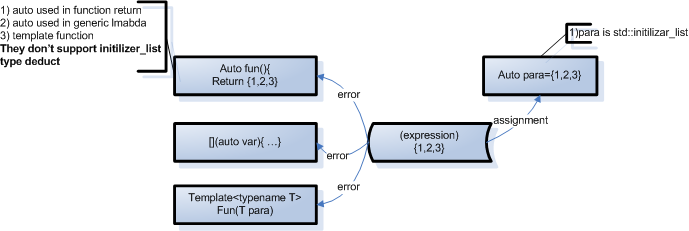
\includegraphics[scale=0.6]{pics/autotype.png}
    \end{center}


\end{itemize}


\subsubsection{auto parameter type deduction}
\begin{itemize}
	\item \texttt{auto} can be used in function parameter, it is just another kind of template function.

\begin{lstlisting}[numbers=none]
void fun1(auto i){
    cout<<i<<endl;
}
		
fun1(23);  //produce two overload fun1 function.
fun1("abc");
\end{lstlisting}

    \item generic lambda( just like template lambda). auto can directly hold closures(lambda), and in C++14, It can be used as lambda parameter.
\begin{lstlisting}[frame=single, language=c++]
auto adder  = [](auto op1, auto op2){ return op1 + op2; };
\end{lstlisting}
	
	\item With help of \texttt{auto}, we can simplify code. 
\begin{lstlisting}[frame=single, language=c++]
auto derefUPLess =               
[](const std::unique_ptr<Widget>& p1,  const std::unique_ptr<Widget>& p2){
	return *p1 < *p2; 
};  //comparison func. for Widgets pointed to by std::unique_ptrs               

//C++14 version, values pointed to by anything pointer-like
auto derefLess = [](const auto& p1,  const auto& p2){
	return *p1 < *p2; 
}; 
\end{lstlisting}
	
	\item \texttt{auto \&\&}is forwarding reference. A good example \texttt{auto\&\&} comes(forwarding reference) from generic lambda. It can reserve rvalue.
\begin{lstlisting}[frame=single, language=c++]
struct Functor{
    void operator ()() const &  { std::cout << "lvalue functor\n"; }
    void operator ()() const && { std::cout << "rvalue functor\n"; }
};

auto perfectLambda = [](auto&& func, auto&&... params) {
	std::forward<decltype(func)>(func)(
	std::forward<decltype(params)>(params)...
	);
};
auto lambda = [](auto func, auto&&... params) {
	func(std::forward<decltype(params)>(params)...);
};

Functor fun;
lambda(fun);  //output  lvalue functor
lambda(Functor{}); //output  lvalue functor
perfectLambda(fun); //output  lvalue functor
perfectLambda(Functor{}); //output  rvalue functor
    \end{lstlisting}

\end{itemize}

\subsubsection{auto return type deduction}
\begin{itemize}
	\item C++11 permits the automatic deduction of the return type of a lambda function whose body consists of only a single return statement, so we don't need to specify its return type.
\begin{lstlisting}[numbers=none]
[=]() -> some_type { return foo() * 42; } // ok
[=]  { return foo() * 42; } //ok,deduces "-> some_type"
\end{lstlisting}
	
	\item In C++14, this has been expanded in two ways. First, it now works even with more complex function bodies containing more than one return statement, as long as all return statements return the same type. Secondly, it now works with all functions, not just lambdas. Of course, this requires the function body to be visible.
\begin{lstlisting}
// C++14
[=] {               // ok, deduces "-> some_type"
	if( expr ) {
		return foo() * 42; // with arbitrary control flow
	}
	return foo() * 43; 
}                       
\end{lstlisting}
		
	\item Below will produce compile error, because it has ambiguity.
\begin{lstlisting}[numbers=none]
auto f(int i){  // It will cause compile error.
    if ( i < 0 )
    	return -1;
    else
    	return 2.0
}
\end{lstlisting}

	\item For template function return type, we can use three different ways.	
	\begin{enumerate}
		\item C++ 11, use auto + trailing type.
\begin{lstlisting}[numbers=none]
template <class T>
auto addFooAndBar(T const& t) -> decltype(t.foo() + t.bar()) {
    return t.foo() + t.bar();
}
\end{lstlisting}

	\item C++ 14, directly use \texttt{auto}.
\begin{lstlisting}[numbers=none]
template <class T>
auto addFooAndBar(T const& t) {
    return t.foo() + t.bar();
}
\end{lstlisting}

		\item Usage of \texttt{decltype(auto)}, I will introduce this topic in \texttt{decltype}. More detail can be found in Effective Modern C++ item 3.
	\end{enumerate}
	
	\item Prefer to use function return type deduction wherever applicable, avoid trailing return type unless you really need them. they make your code harder to read.
	
	\item There are three ways to view deducted type. You can use IDE or use \texttt{typeid} or \\ \texttt{std::type\_info::name}. Another trick is to use compiler error message.

\begin{lstlisting}[frame=single, language=c++]
template<typename T> // declaration only for TD;
class TD; // TD == "Type Displayer"

TD<decltype(x)> xType; 
TD<decltype(y)> yType; 
//elicit errors containing x's and y's types

std::cout << typeid(x).name() << '\n';  //use typeid 
\end{lstlisting}
		
\end{itemize}



\subsection{decltype deduction}
\subsubsection{basic deduction rule}
\begin{itemize}
	\item decltype has two different deducting rules when facing different kinds of expression.
	
	\begin{enumerate}
		\item Expression whose type is to be determined is \textbf{a plain variable} or \textbf{function parameter}, like \texttt{x}, or a class member access, like \texttt{p->m\_x.} In that case, decltype lives up to its name: it determines the type of the expression to be the declared type.  Pay attention to the difference between \texttt{decltype} and \texttt{auto}.
\begin{lstlisting}[frame=single, language=c++]
vector<int> v; // decltype(v) is vector<int>
struct S {
	int m_x;
};

int x;
const int cx = 42;
const int& crx = x;
const S* p = new S();

decltype(x) a;  // a is int, as auto a =x

decltype(cx) b; // b is const int
auto b = cx;  //auto ignore const, b is int

decltype(crx) c;  // c is const int&.
auto c = crx; //ignore reference and const, c is int

decltype(p->m_x) d; // d is int although p points to const S
auto d = p->m_x; //auto ignore const, d is int
\end{lstlisting}
		
		\item If expr is not case 1, then it's case 2. There are three different rules for case 2:
		\begin{enumerate}
			\item If expr is an lvalue, then \texttt{decltype(expr)} is \texttt{T\&}. 
			\item If expr is an xvalue, then \texttt{decltype(expr)} is \texttt{T\&\&}. 
			\item Otherwise, expr is a prvalue, and \texttt{decltype(expr)} is \texttt{T}.
		\end{enumerate}
	\end{enumerate}


	\item For case 2, some complex expression examples:
\begin{lstlisting}[frame=single, language=c++]
const S foo();
const int& foobar();
std::vector<int> vect = {42, 43};

typedef decltype(foo()) foo_type;   //const S
typedef decltype(foobar()) foobar_type; //const int&
decltype(vect[0]) first_element = vect[0]; //const int&
double d1, d2;
typedef decltype(d1 < d2 ? d1 : d2) cond_type; //double &
int x = 0;
typedef decltype(x < d2 ? x : d2) cond_type_mixed;  //double
\end{lstlisting}

	\begin{description}
		\item[Line 5:] \texttt{foo()} is declared as returning \texttt{const S}. The type of \texttt{foo()}
is \texttt{const S}. Since \texttt{foo()} is a prvalue, decltype does not add a reference. Therefore, \texttt{foo\_type} is \texttt{const S}.
		
		\item[Line 6:] The type of \texttt{foobar()} is \texttt{const int\&}, and it is an lvalue. Therefore, decltype adds a reference. By the C++11 reference collapsing rules, that makes no difference. Therefore, \texttt{foobar\_type} is \texttt{const int\&}
		
		\item[Line 7:] \texttt{std::vector<int>}'s operator[] is declared to have return type \texttt{int\&}. Therefore, the type of the expression \texttt{vect[0]} is \texttt{int\&}. Since \texttt{vect[0]} is an lvalue, decltype adds a reference. By the C++11 reference collapsing rules, that makes no difference. Therefore, \texttt{first\_element} has type \texttt{int\&}.  
		
		\item[Line 9:]  The type of the expression is double, and the expression is an lvalue. Therefore, a reference is added, and \texttt{cond\_type} is \texttt{double\&}
		
		\item[Line 11:] The type of the expression is double. The expression is a prvalue, because in order to accommodate the promotion of x to a double, a temporary has to be created. Therefore, no reference is added, and \texttt{cond\_type\_mixed} is \texttt{double}.  For a conditional expression (?:) to be an lvalue (again, in broad and simple terms), the second and third operands must be lvalues of the same type. This is because the type and value category of a conditional expression is determined at compile time and must be appropriate whether or not the condition is true. If one of the operands must be converted to a different type to match the other then the conditional expression cannot be an lvalue as the result of this conversion would not be an lvalue.
	\end{description}

\end{itemize}

\subsubsection{decltype usage}
\begin{itemize}
		
	\item decltype case 2 rule mainly used in deducting template function return value. In C++ 14, we can use auto directly.
\begin{lstlisting}[frame=single, language=c++, mathescape=true]
template<typename T, typename U>  //C++ 11
auto eff(T t U u) -> decltype(T*U){
....
}

template<typename T, typename U> //after C++ 14
auto eff(T t U u) {
	return t*u
}
\end{lstlisting}

	\item Also in C++14, we got generic lambdas. Those are basically lambdas with a templated function call operator, but we don’t get to declare any template parameters. Actually working with the type of whatever was passed to the lambda requires decltype.
\begin{lstlisting}
auto make_multiples = [](auto const& x, std::size_t n) { 
	return std::vector<std::decay_t<decltype(x)>>(n, x); 
};	
\end{lstlisting}

%	\item When a function returns a lvalue reference, auto will not work here(skip reference), only decltype can keep reference properly.
%\begin{lstlisting}
%template<typename Container, typename Index>  //C++11 syntax
%auto authAndAccess(Container& c, Index i) -> decltype(c[i]){
%	authenticateUser();
%	return c[i];
%}
%
%template<typename Container, typename Index> // C++14 syntax
%decltype(auto) authAndAccess(Container& c, Index i) {  //decltype(auto) here
%	authenticateUser();                               
%	return c[i];
%}
%\end{lstlisting}

		\item When you use \texttt{decltype(auto)}, it tells the compiler to automatically perform type deduction, but to use \texttt{decltype} rules. This is most useful when dealing with expressions that return an lvalue, such as \texttt{a[0]}. In this case, if you use \texttt{auto}, it will ignore any reference, but \texttt{decltype(auto)} will preserve it. Below is example about using decltype(auto). The whole code need extra explanation here:
	\begin{enumerate}
		\item Need \texttt{Container\&\& c} to accept both lvalue and rvalue.
		\item Inside function, \texttt{c} need to be forward. that is common rule for forwarding reference.
		\item Forward return xvalue, then when we return this value, we also need keep it as xvalue.
		\item That is why decltype rule come from: "If expr is an xvalue, then \texttt{decltype(expr)} is \texttt{T\&\&}".
		\item Outside of function, return is xvalue, so we can move it efficiently. that is the whole story for the below code. 
	\end{enumerate}
\begin{lstlisting}[frame=single, language=c++, mathescape=true]
template<typename Container, typename Index> // final c++11
auto authAndAccess(Container&& c,Index i)
         ->decltype(std::forward<Container>(c)[i]){
	authenticateUser();
	return std::forward<Container>(c)[i];
}

template<typename Container, typename Index> // final c++14
decltype(auto) authAndAccess(Container&& c, Index i) {
	authenticateUser();
	return std::forward<Container>(c)[i]; //if c is xvalue, c[i] is too
}

auto s = authAndAccess(queue,5); //copy here.
auto s = authAndAccess(std::move(queue),5);  //move here
\end{lstlisting}

	\item Another example of usage of \texttt{decltype(auto)}. \texttt{array[pos]} in below code is lvalue. \texttt{decltype(auto)} will make the return type is \texttt{int\&}, not \texttt{int}. So we can get the desired effect. 
\begin{lstlisting}
template <typename T>
decltype(auto) array_access(T& array, size_t pos)  {
	return array[pos]; //return int& here, 
}

std::vector<int> vect = {42, 43, 44};
int* p = &vect[0];  //* dereference operator return &
array_access(p, 2) = 46; //we can modify vect here. 44 is changed to 46.	
\end{lstlisting}
	
	\item The use of \texttt{decltype(auto)} is not limited to function return types. It can also be convenient for declaring variables when you want to apply the decltype type deduction rules to the initializing expression.
\begin{lstlisting}[frame=single, language=c++, mathescape=true]
Widget w;
const Widget& cw = w;
auto myWidget1 = cw;  //auto type deduction: myWidget1's type is Widget.
decltype(auto) myWidget2 = cw; //myWidget2's type is  const Widget&
\end{lstlisting}

	\item An important property of decltype is that its operand never gets evaluated. For example, you can use an out-of-bounds element access to a vector as the operand of decltype with impunity:
	
\begin{lstlisting}[frame=single, language=c++, mathescape=true]
std::vector<int> vect;
assert(vect.empty());
typedef decltype(vect[0]) integer;  //work even vect is empty.
\end{lstlisting}
	
	\item Another property of decltype is that when decltype(expr) is the name of a plain user defined type (not a reference or pointer, not a basic or function type), then decltype(expr) is also a class type name. This means that you can access nested types directly:
\begin{lstlisting}[frame=single, language=c++, mathescape=true]
template<typename R>
class SomeFunctor {
public:
	typedef R result_type;
	result_type operator()() {
		return R();
	}
SomeFunctor(){}
};

SomeFunctor<int> func;
typedef decltype(func)::result_type i; //i is int, You can access nested type
\end{lstlisting}
	
	\item You can also declaring variables by \texttt{decltype}. Note that you can't use auto in this case. This is because \texttt{decltype} doesn't actually execute the expression given as its argument; it is only used by the type checker to determine a type. This usage is similar to using \texttt{auto a = expression}, where we can automatically deduce the type of a from the expression.
\begin{lstlisting}[frame=single, language=c++, mathescape=true]
class A {
	std::vector<std::pair<int, std::string>> array;
	decltype(array.begin()) iter; 
	//Don't need to use: std::vector<std::pair<int, std::string>>::iterator iter 
};
\end{lstlisting}
\begin{description}
	\item[Line 3:] You don't need initialization expression here. you can't use auto here, because auto need initialization expression
\end{description}
	
	\item We could have also done the above example with \texttt{declval}. It allows you to use decltype without constructing the object. The type doesn't even need a default constructor, and in fact, it can be used with an incomplete type. The above example could be rewritten as:
	
\begin{lstlisting}[frame=single, language=c++, mathescape=true]
template <typename C>
decltype(std::declval<const C>().begin()) //make sure that C has begin() function.
foo(const C& c){
	return one iterator of c
}
\end{lstlisting}
	
	\item \texttt{declval} is commonly used in templates where acceptable template parameters may have no constructor in common, but have the same member function whose return type is needed.
	
\begin{lstlisting}[frame=single, language=c++]
struct Default {
	int foo() const { return 1; } 
};

struct NonDefault{
NonDefault(const NonDefault&) { }
int foo() const { return 1; }
};
	
decltype(Default().foo()) n1 = 1;    //type of n1 is int
//decltype(NonDefault().foo()) n2 = n1;  //doesn't work, no default ctor
decltype(std::declval<NonDefault>().foo()) n2 = n1; //It's OK now, n2 is int
\end{lstlisting}
	
%	\item However, the reference that \texttt{decltype} adds is not always what you want. It happens frequently that you need to remove it with \texttt{remove\_reference}. 
%\begin{lstlisting}
%template<typename T, typename S>
%auto fpmin(T x, S y) -> decltype(x < y ? x : y) {
%	return x < y ? x : y;  //If x and y have same type, it return reference.
%}  						//Return reference of local object is always HORRIBLE!.
%
%template<typename T, typename S>
%auto fpmin(T x, S y) 
%	->typename std::remove_reference<decltype(x<y?x:y)>::type{
%	return x < y ? x : y;
%} //Correct implementation.
%\end{lstlisting}	
	
	\item Basic knowledge of decltype detail can be found "How decltype Deduces the Type of an Expression: Case 1"

\end{itemize}

\subsection{Type deduction summary}
\begin{itemize}
	\item \texttt{auto}, template T and decltype are three kinds of type deduction contexts. \texttt{auto} and template T are almost same, except when we encounter \texttt{initilizaer\_list}.  

	\begin{center}
		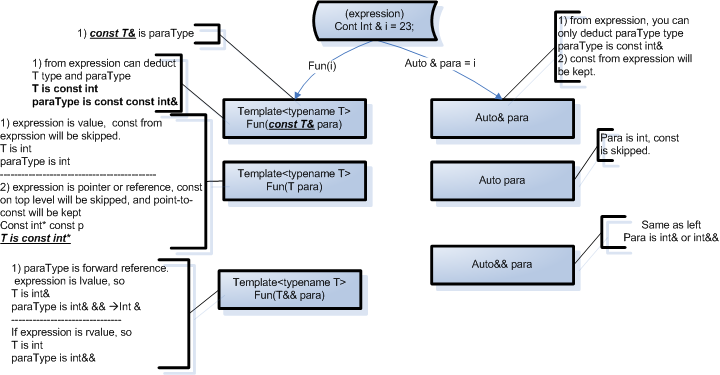
\includegraphics[scale=0.6]{pics/type_deduct.png}
	\end{center}

	
	
	\item Why \texttt{decltype} has so complex definition about type deduction?  There are two different ways in which decltype(expr) can work, depending on the value of the category of the expression. The final specification of decltype represents a compromise between two different possible points of view. \texttt{decltype} Rule 1 is for declaring a variable, and \texttt{decltype} Rule 2 is for deducing the type for the return value from a function.
	\begin{enumerate}
		\item Rule 1 is that decltype should be a way to retrieve and reuse the type of a variable as declared in the source code: I declared a variable x of type T at some point in my code. Now I want to use that type for some other purpose, like making a typedef, or specify the return type of a function. I don't want to repeat myself, so give me a way to recover the declared type of my variable, exactly the way I originally wrote it. If that declared type has a reference and/or a const or volatile qualifier on it that I don't want, I'll remove that myself. This is what Case 1 of the specification of decltype does.
		
		\item Rule 2 originates in the needs of library writers. They often find themselves in a situation where the return type of a function needs to be the type of some expression, typically something that depends on template parameters. When the return expression is \texttt{T[]}, we need to return an lvalue reference because it's an lvalue. When the return expression is \texttt{std::move()}, we need to return \texttt{T\&\&} because it's an xvalue. For the remaining 99\% of expressions, such as T1+T2, they return prvalues, so we just return the type for the prvalue, That is all!
	\end{enumerate} 
	
	\begin{center}
		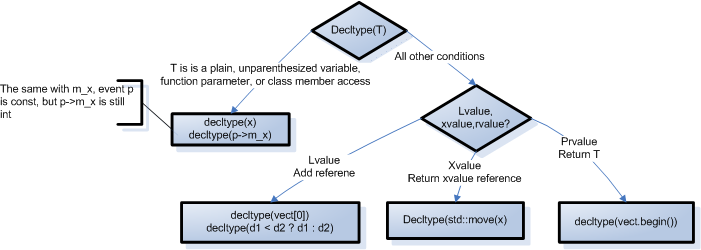
\includegraphics[scale=0.65]{pics/decltype.png}
	\end{center}
	
	 \item \texttt{decltype} is quite different from auto and template T. It can be used in a wider variety of contexts, such as typedefs, function return types, and even in places where a class name is expected.
	 \begin{enumerate}
	 	\item Return type deduction in C++11, which was deprecated in C++14.
	 	\item Use \texttt{decltype(auto)} to maintain the reference type.
	 	\item Generic lambda type deduction.
	 	\item Declare variable type without initialization expression, which is slightly different from auto. It has some advantages; it doesn't require executing the code and can be combined with \texttt{declval}.
	 \end{enumerate}
	

	
\end{itemize}

\section{template specialization}
\subsection{class template specialization}
\begin{itemize}
	\item Class templates can be partially specialized, and the resulting class is still a template. Partial specialization allows template code to be partially customized for specific types in situations, such as:

	\begin{enumerate}
		\item A template has multiple types and only some of them need to be specialized. The result is a template parameterized on the remaining types.

		\item A template has only one type, but a specialization is needed for pointer, reference, pointer to member, or function pointer types. The specialization itself is still a template on the type pointed to or referenced.
		
		\item There are three types of partial specialization. Please note that all partial specialization forms must have <> after the class name.
		\begin{enumerate}
			\item specialize one or more of types.
\begin{lstlisting}[frame=single, language=c++]
template<class T1, class T2>
class A{
}

template<class T1>
class A<T1, int>{  // must have <> after class name
}		
\end{lstlisting}				
			
			\item specialize to point or reference type.
\begin{lstlisting}[frame=single, language=c++]
template<class T>
class A{
}

template<class T>
class A<T*>{  // must have <> after class name
}		
\end{lstlisting}	
			\item specialize to another template.
\begin{lstlisting}[frame=single, language=c++]
template<class T>
class A{
}

template<class T>
class A<vector<T> >{  // must have <> after class name
}			
\end{lstlisting}	

		\end{enumerate}
	
		\item Here's another example of class template specification. You can see that there are three levels which become narrower and narrower: 1) the base template, 2) partial specialization, and 3) explicit (full) specialization of the member.
\begin{lstlisting}[frame=single, language=c++]
template <class T>  // 1)base template
class Storage{
	T m_value;
public:
	Storage(T value){
	m_value = value;
}

template <class T> // 2)partial specialization
class Storage<T*>{ //There is <> after class name.
	T* m_value;
public:
Storage(T* value){
	m_value = new T(*value);  //To make deep copy
}

template <>  //3) explicit(full) specialization, empty <> after template
Storage<char*>::Storage(char* value){
	int length = 0; //Figure out how long the string in value is
	while (value[length] != '\0')
		++length;
}
\end{lstlisting}

\end{enumerate}

    \item Always keep the design of a template in mind and avoid blind use. When you use a pointer as a typename, be on high alert. If a common template cannot handle a pointer type very well, you can define a partial specialization. Please note that the declaration of specialization should come after the basic template.

\begin{lstlisting}[frame=single, language=c++]
template <typename T>
class Foo //general one

template <typename T>
class Foo<T*> //partial specializations.
\end{lstlisting}

\end{itemize}

\subsection{Function template specification}
\subsubsection{Basic knowledge about function template specification}
\begin{itemize}

    \item In the case of a template function, there are overload and full specialization options, while for a template class, there are full and partial specialization options. Template functions do not support partial specialization because they can use overloading to achieve the same result. In other words, if you want to have a custom implementation of a function with the same name, you should use an overloaded function. However, if you need a custom implementation of a class with the same name, you can use partial or full specialization.
    
	\item You can also explicit(full) specialization of member in template class. 


    \item Explicit Specialization: Because for \texttt{char *}, you can't use >, but you can use \texttt{strcmp}. Therefore, you need to build an explicit specialization version. The prototype and definition of an explicit specialization should be preceded by \texttt{template<>} and should mention the specialized type by name."
    
\begin{lstlisting}[numbers=none]
Template<typename T>  //template function
void sortedArrary(T) {...};

template<> void sortedArray<const char *>(){...}
\end{lstlisting}

	\item Some explicit specification syntax.
\begin{lstlisting}[frame=single, language=c++]
template<typename T>
void foo(T param);

void foo(int param); //regular funciton, not a specialization. it is an overload
void foo<int>(int param); //ill-formed, not recommend, no template keyword at all

template <> void foo<int>(int param){...} //normal explicit specialization
template <> void foo(int param); {...} //same as above, skip<int>

template void foo<int>(int param); //explicit instantiation, normal 
template void foo<>(int param); //explicit instantiation, skip type
template void foo(int param);  //explicit instantiation, skip <type>
\end{lstlisting}

\end{itemize}

\subsubsection{overload or full specification of function template}

\begin{itemize}
	\item  If you want to customize a function base template and want that customization to participate in overload resolution (or, to always be used in the case of exact match), make it a plain old function, not a specialization. And, if you do provide overloads, avoid also providing specializations. Detail you can google" Why Not Specialize Function Templates?" prefer to use overload than template function specification.

	\item For a function template, we pick which function to use in the following order: 1) Pick one from the overloaded function templates; 2) Pick the specialized version of the function template that was chosen in the first step.

\begin{lstlisting}[frame=single, language=c++]
template<typename T>
f(T t);  //#1

template< >f<int*>(int* t) #2

template<typename T>
f(T* t); //#3

template<> f<int> f( int* t) //#4

int * p;
f(p) // #4>#3>#2>#1
\end{lstlisting}
\begin{description}
	\item[Source code:] The First step, we picked \texttt{f(T* t)} function template \#3, then select a specialization of this funciton template \#4. The \#1 and \#2 are not considered at all. Please note here \#3 is not \#1 partial specialization, but overload version. 
\end{description}

	\item For above example, If you omit type inside <> after function name f, it depends on location.
\begin{lstlisting}[frame=single, language=c++]
template<typename T>
f(T t);  //#1

template< > f<>(int* t) //#2 is specialization of #1

template<typename T>
f(T* t); //#3
//template< > f<>(int* t) //If we put here, #2 is specialization of #3

int *p; 
f( p ); 
\end{lstlisting}
\begin{description}
	
	\item[Line 11:] If put specialization version(\#2) at line 4, it will call \#3. Although we have a very match specification, it's not be picked up and it's not what we want.  Why this happen? \textbf{because specification didn't join the overload processing, this will lead to a missing match specification.} The first, we only see two overload template functions: \texttt{f(T t)} and \texttt{f(T* t)}. In this way, \texttt{f(T* t)} is picked up. If we put specification version(\#2)  in line 4, then it is specification of \#1, that is why it's omitted. If put specialization version(\#2) at line 8, it will be called because compiler think that it's the full specialization of \#3	
\end{description}

	\item Why do we need an overloaded template function? Because not all types support the same operations. For example, in your template function, you may use the = operator for assignment, but when you use an array as the type argument for this template function, arrays don't support assignment with the = operator.
\begin{lstlisting}[numbers=none]
template <typename T>
void swap(T a[], T b[], int n)

template <typename T> //overload previous functions
void swap(T &a, T &b )
\end{lstlisting}

	\item Overload is different with Specializations, Overload means that you have different function signatures. Specialization have the same function signature.

	\item Explicit specializations usually need define all the implementation in it. If there is a lot of repetition. There are two helpful options: 
\begin{enumerate}
	\item Add a special function which is just suitable for certain type. 
\begin{lstlisting}[numbers=none]
template <typename T>
class A{
public:
	void onlyForInts(T t){
		static_assert(std::is_same<T, int>::value, "Only ints!");
	}
};

A<int> i;
i.onlyForInts(1); // works !
A<float> f;
//f.onlyForInts(3.14f); // does not compile !
\end{lstlisting}

	\item Use type trait and overload, select at the compile time. See \texttt{enable\_if} example below.
\end{enumerate}

    \item pointer sometimes need to be deal with differently, at that time we need partial specialization of template class. A very good article is:\\ https://www.learncpp.com/cpp-tutorial/13-8-partial-template-specialization-for-pointers/. 

    \item Another good articles about specialization is chapter 12 in "C++ template: The complete guide", you should read each sentence in this chapter. Other good articles are: "Why Argument Dependent Lookup doesn't work with function template dynamic\_pointer\_cast"; "C++ template function taking template class as parameter".
\end{itemize}


\section{Template instantiation}

\subsection{Difference between instantiation and specification}
\begin{itemize}
    \item Implicit, explicit instantiation, and explicit specialization are all forms of specialization. Because they produce real function definitions that use specific types, the final result is not a template at all. On the contrary, partial specialization is different from explicit (full) specialization. Partial specialization makes the generic template more specific, but the result is still a template.
    
    \item For class template, specialization includes explicit(full) specialization and partial specialization. They all need to give new implementation. For function template, there is no partial specialization, So explicit specialization is complete specialization. 
\begin{lstlisting}[frame=single, language=c++]
template<> class Pair<int,int>{...}; // full specialization 
template<typename T1> class Pair<T1, int>{...}; //partial specialization 	
\end{lstlisting}    

	\item Instantiation happens at compile time, not at run time. When you declare a variable, it will be instantiated, which may increase the compiling time. Therefore, all template definitions must be put into a header file.
    
   	\item There seems to be (a lot) of confusion regarding explicit instantiation and specialization. Instantiation has no empty <> after template, and you don't need to give definition of function or class. explicit specialization has empty <> after template, and you need to give out definition.
\begin{lstlisting}
template <typename T> void func(T param) {} // definition

template void func<int>(int param);  //explicit instantiation. no definition.
template <> void func<int>(int param){} 
// empty <> here, explicit specialization, has definition.
\end{lstlisting}    

   
	\item C++ uses implicit or explicit instantiation to generate a specialized class or function definition from a template. For implicit instantiation, you have to declare a variable, but for explicit instantiation, you don't need to declare an object. Instead, you can either declare a variable or use the template keyword. Both types of instantiation are based on an existing template implementation.
	
\begin{lstlisting}[frame=single, language=c++]
template<typename T, int n>
class ArrayTP...
	
ArrayTP<int, 100> stuff //implicit instantiation, define a variable, 	
template ArrayTP<string, 100>; //explicit instantiation, use template keyword and< >, 

template<>      //explicit specialization, empty <> here
ArrayTP<bool, 100>{...specific implementation} //there is implementation here.	
\end{lstlisting}

%	\item Non type argument and default type argument only define one template body(only one recipe). But specialization need to define a generic template body(one recipe), For another type, It need to define a different template body(another recipe), because the code will be different with generic one.
	 
%	 \textbf{Instantiation is different with specialization.  For instantiation, it will use template function to produce function body, but for specialization, you have to redefine you own function body }
%	 
%\begin{lstlisting}[frame=single, language=c++]
%Template<typename T>
%void sortedArrary (T t) {...};
%
%template void sortedArray<Person>(Person);
%
%template<> void sortedArray<Person>(Person t){  //it is full specialization.
%.... //give you own definition of template fun body.
%};
%.
%\end{lstlisting}

	
\end{itemize}

\subsection{overload resolution rule}
\subsubsection{Name look up and resolution rule}
\begin{itemize}
    \item A name is a qualified name if the scope to which it belongs is explicitly denoted using a scope-resolution operator (::) or a member access operator (. or ->). For example, \texttt{this->count} is a qualified name.

    \item  A name is a dependent name if it depends in some way on a template parameter.  For example, \texttt{std::vector<T>::iterator} is usually a dependent name if \texttt{T} is a template parameter, but it is a nondependent name if \texttt{T} is a known type alias (such as the \texttt{T} from \texttt{using T = int}).

	\item Qualified names are looked up in the scope implied by the qualifying construct. If that scope is a class, then base classes may also be searched. However, enclosing scopes are not considered when looking up qualified names. 

	\item In contrast, unqualified names are typically looked up in successively more enclosing scopes (al-though in member function definitions, the scope of the class and its base classes is searched before any other enclosing scopes). This is called ordinary lookup. A more recent twist to the lookup of unqualified names is that—in addition to ordinary lookup—they may sometimes undergo argument-dependent lookup (ADL).
            
    \item \textbf{compiler will parse the template definition before it instantiation.} Why? It's a compiler, not a macro processor. Errors in the template itself won't be detected as long as it is only instantiated with 'friendly' types that don't trigger the errors: for example, if the template assumes that the type always has such-and-such a method.

    \item C++ Coding standards 65 states customization of point. In order to understand it. You need to understand two basic conceptions: \textbf{"two phases lookup"} and \textbf{"dependent name"}.  Two phases lookup can see "Dependent name lookup for C++ templates" and "Two-Phase or Not Two-Phase: The Story of Dependent Names in Templates". Just google them.

	\item Given a function name, you can have regular, template and explicit specialization template. When pick a function, regular> specialization> template. function picking ranking from best to worst is: 
		1) Exact math, regular function.
		2) Template if you have define the same template function name.
		3) Conversion by promotion.
		4) Conversion by standard conversion.
		5) user-defined conversion.

	\item What is exact match. There are table below:

\begin{center}
	\begin{tabular}{|c|c|}
	\tophline
	Actual argument & Formal argument \\
	\tophline
	type-name & type-name \& \\
	\tophline
	type-name \& & type-name \\ \tophline
	type-name [ ] &  type-name* \\ \tophline
	type-name ( argument-list ) & ( *type-name ) ( argument-list ) \\ \tophline
	type-name  & const(volatile) type-name \\ \tophline
	type-name*  & const(volatile) type-name*  \\ \tophline
	\end{tabular}
\end{center}

	\item About exact match, there are three rules to follow:
	\begin{enumerate}
		\item If there are two exact matches, compiler can't distinguish them, then it will report error.
		
		\item If reference and pointer, even there are two exact match, It will pick up first according to const.
\begin{lstlisting}[frame=single, language=c++]
f(const int& j); //#1
f(int& j);  //#2, 

int i = 2;
f(i)  //Here, #2 will be selected, because i isn't const.
\end{lstlisting}

		\item If there are exact match, it will pick up before template, even template has EXACT specification.
\end{enumerate}

	\item You can explicitly tell compiler that you prefer template function over overload one.

\begin{lstlisting}[frame=single, language=c++]
template<typename T>
void f(T t);  //#1
void f(int t) //#2
f<>(2); // tell compiler to use #1
\end{lstlisting}

%    \item Overload resolution steps are introduced here. More explanation of this figure can be found below from code p1 to code p6:
%
%\begin{figure}[ht]
%	\centering 
%	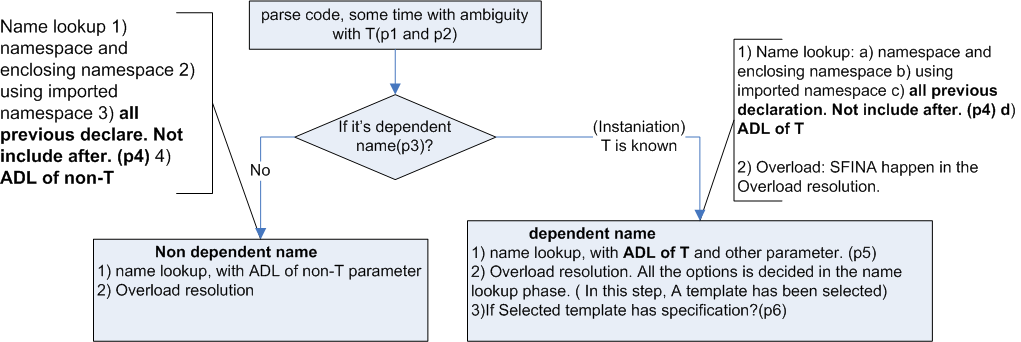
\includegraphics[width=0.8\linewidth]{pics/template.png}
%	\caption{Template name look up}
%	\label{fig:command}
%\end{figure}



	\item In the below two examples, since both are dependent names, we have to add an extra typename and template keyword to help the parser resolve the ambiguity. It's important to note that the typename keyword is mandatory before a qualified, dependent name that refers to a type.

\begin{lstlisting}[frame=single, language=c++]
template <typename T> struct Base {
	typedef int MyType;
};

template <typename T> struct Derived : Base<T> {
	void g() {
		// MyType k = 2;  //error: 'MyType' was not declared in this scope
		// Base<T>::MyType k = 2; //Error, MyType is a dependent name.	
		// Base<T>::MyType* k = 2; //Ambiguity here, * maybe a multiple operator.
		typename Base<T>::MyType k = 2; //work, 
	}
};
\end{lstlisting}
\begin{description}
		
	\item[Line 10:] When the compiler parses the template code in this line, no real instantiation is visible. Therefore, you should inform the compiler that \texttt{::MyType} is a type name, not a variable name or anything else. This will allow us to use it to declare a variable \texttt{k}.
\end{description}

\begin{lstlisting}[frame=single, language=c++]
struct Foo {
	template<typename U>
	static void foo_method(){
	}
};

template<typename T> void func(T* p) {
	// T::foo_method<T>(); // error: expected primary-expression before '>' token	
	T::template foo_method<T>(); //work!. That is "template qualifier".
}
\end{lstlisting}

	\item If some names are not dependent names, we don't perform a "two-stage name lookup"; we just look for the name in the visible scope and all the previous source code.
\begin{lstlisting}[]
template <typename T> struct Base {
   void f() {...}
};

template <typename T> struct Derived : Base<T> {
 void g() {
     f();  //error happen here. 
     this->f();  //work, become dependent name, delay the name lookup after instantiation.
 }
};
\end{lstlisting}
\begin{description}
	\item[Line 7:] \texttt{f()} is not dependent name, so we begin to look for this name now, but the base class doesn't still exit (no instantiation yet), so report error.
\end{description}


	\item Dependent name looking up has two stages. There are two variant version of below code, If you define \texttt{VAR1}, then line 33 and 34 will output "master". The explanation is below:
\begin{enumerate}
	\item From \texttt{process} function, it looks for \texttt{f} function. It looks for 1)Current namespace. 2)Using namespace. 3)All previous declaration.
	At these time only \texttt{f(T)}(line 3) is visible, Then add it into overload options set.  
	
	\item Because in the \texttt{f(v)}(line 6), v is dependent name. When T is knowing \\ (\texttt{optional<int>}), It will search the name \texttt{f} in the \texttt{boost} namespace again and found there are no any name \texttt{f} there.  At this time, it will not search framework namespace again.
	
\end{enumerate}	

	If you don't define \texttt{VAR1}, then the line 33 and 34 will output  "optional<T>" and "optional<bool>" seperately. The explanation is below:
	
	\begin{enumerate}
		\item In line 6, we see the \texttt{f(v)}, then we just use \texttt{non-concrete-type} lookup. At this time only a \texttt{f} definition in line 3 is visible.
		
		\item In line 33, When you see \texttt{ob}, we can use \texttt{concrete-type} lookup, at this time, first, we extract concrete-type(\texttt{optional} type), then we look for boost namespace which optional type resides in. In this namespace, we found two other functions options(line 21 and line 23), then we add them to overload options. 
		
		\item In line 34, Once we finish overload resolution, If we select template function, then we use concrete-type specialization look up, looks all the options before line 34. That is why we select specialization in line 23.
	\end{enumerate}	

\begin{lstlisting}[]
namespace framework { // library 1
	template <typename T>
	void f(T) { puts("master");}
 
	template <typename T>
	void process(T v) { f(v); } //v is dependent name.
}
 
namespace boost {     // library 2
	template <typename T>
	struct optional {};
}

#ifdef VAR1 
namespace framework { 
#else
namespace boost {
#endif

	template <typename T>
	void f(boost::optional<T>) { puts("optional<T>"); }
    
	inline void f(boost::optional<bool>) 
	                { puts("optional<bool>"); }
}
 
int main(){
	int i = 0;
	boost::optional<int>  oi;
	boost::optional<bool> ob;
  
	framework::process(i); //output three "master"
	framework::process(oi);
	framework::process(ob);
}
\end{lstlisting}


%	\item p5, In instantiation, with help of ADL, boost namespace is searched and two other functions are added into overload options.
%\begin{enumerate}
%	\item In line 6, we see the \texttt{f(v)}, then we just use \texttt{non-concrete-type} lookup. At this time only a \texttt{f} definition in line 3 is visible.
%	
%	\item In line 28, When you see \texttt{ob}, we can use \texttt{concrete-type} lookup, at this time, first, we extract concrete-type(\texttt{optional} type), then we look for boost namespace which optional type resides in. In this namespace, we found two other functions options(line 15 and line 18). Add them to overload options. 
%	
%	\item In line 29, Once we finish overload resolution, If we select template function, then we use concrete-type specialization look up, looks all the options before line 29. That is why we select specialization in line 18.
%\end{enumerate}	
%
%\begin{lstlisting}[]
%namespace framework{  // library 1
%  template <typename T>
%  void f(T) { puts("master"); }
% 
%  template <typename T>
%  void process(T v) { f(v); } 
%}
% 
%namespace boost{      // library 2
%  template <typename T>
%  struct optional {};
%}
% 
%namespace boost {      // some glue between 1 and 2
%  template <typename T>
%  void f(optional<T>) { puts("optional<T>"); }
%    
%  inline
%  void f(optional<bool>) { puts("optional<bool>"); }
%}
% 
%int main(){
%  int i = 0;
%  boost::optional<int>  oi;
%  boost::optional<bool> ob;
%  
%  framework::process(i);
%  framework::process(oi); //output "optional<T>"
%  framework::process(ob); //output "optional<bool>"
%}
%\end{lstlisting}
%
%	\item p6, template specification happen in the end and after overload. 
%\begin{lstlisting}[]
%namespace framework{  // library 1
%  template <typename T>
%  void f(T) { puts("master"); }
% 
%  template <typename T>
%  void process(T v) { f(v); } 
%}
% 
%namespace boost{      // library 2
%  template <typename T>
%  struct optional {};
%}
% 
%namespace framework{  // some glue between 1 and 2
%  template <>
%  void f<boost::optional<bool>>(boost::optional<bool>)
%  { puts("optional<bool>"); }
%}
% 
%int main() {
%  int i = 0;
%  boost::optional<bool> ob;
%  
%  framework::process(i); //output master
%  framework::process(ob); //output "optional<bool>"
%}
%\end{lstlisting}
			
		\item Pay attention, you can't put the specialization after calling points, otherwise it will report error. 
\begin{lstlisting}
template <typename T>
void f(T) { cout<<"master"<<endl; }

int main(){
int i = 2;
f(i);
}

template<> void f<int>(int i){ //error
cout<<"specialization"<<endl;
}
\end{lstlisting}
\begin{description}
	\item[Source code:] In line 6, compiler will generate \texttt{f(int)}, when it processes to line 9 and see another \texttt{f(int)}, it reports a kind of "duplicate" error
\end{description}


	\item Another interesting example helps you to understand previous all the examples. You can copy this code and run it, to try different combination and see the output. Please refer the previous figure and all the source examples form p1 to p6. 
\begin{lstlisting}[frame=single, language=c++, numbers=left,
stepnumber=1,]
template<typename T>
void f(T i){
	cout<<"template "<<i<<endl;
}

//template<> void f<short>(short s);
void g(void){
	//int s = 5; //output template
	short s = 5; 
	//uncomment above specification, call specification version.

	//"Specification after initialization.
	f(s);
}

template<> void f<short>(short s){
	cout<<"specification" <<s <<endl;
}
void f(short s){
	cout<<"short " <<s<<endl;
}

int main(){
	g();
}
\end{lstlisting}

\begin{enumerate}
	\item put line 19 and line 16 two functions before function \texttt{g}, it will call regular exact match function \texttt{void f(short)}. 
	
	\item put \texttt{void f(short)} after function g, it will can full specification version
	
	\item comment line 6 (specification declaration). report error:\\
	error: specialization of 'void f(T) [with T = short int]' after instantiation.
	Because it has instantiation f(short) version from generic template, you can't specialize it any more.
	 
	\item Although exact match and specification have higher order, but you you must make it visible by declaring them before the caller.
\end{enumerate}

	\item \textbf{Summary of name look up}: 
	\begin{enumerate}
		\item For both dependent names and non-dependent names, we perform non-concrete-type lookup in the visible scope and previous source code.
		
		\item For dependent names, once we reach the instantiation code, we will know the concrete type, and then we will perform concrete-type ADL (argument-dependent lookup) lookup. 
		
		\item Once we select a template function in the overload, we will look to see if we have a concrete-type specialization version.
	\end{enumerate}

    \item A good article is "Overload resolution" in Andrzej's C++ blog. It taught you 1) name lookup and 2)overload and 3)instantiation three conception very well.
\end{itemize}

\section{Common used template technologies}

\subsection{template parameter}

\begin{itemize}
	\item You should use templates if you need functions or container classes (such as those that act like) that apply the same algorithm to a variety of types. Templates are frequently used for container classes because the concept of type parameters matches well with the need to apply a common storage plan to a variety of types.
\begin{lstlisting}[numbers=none]
template<typename T> //good style, use typename and simple name, such as T
//template<class COMPLEX_T> //bad style, don't use class and complex name
swap(T& a, T&b){	
\end{lstlisting}
	\item You can have several kinds of template parameters.
	\begin{enumerate}
		\item  Type Parameters: 1)Types, 2) Templates (only classes and alias templates, no functions or variable templates. Because neither function nor variable templates are type.)
		
		
		\item Non-type Parameters: 1)Pointers, 2)References, 3)Integral constant expressions. (That is why \texttt{constexpr} is so important.)	
	\end{enumerate}

        \item You can use more than one type parameter, or default type template parameters.
\begin{lstlisting}[numbers=none]
template <typename T1,  typename T2>
class Pair{ };
Pair<double, int> pair1; //two type parameters.

template <typename T1,  typename T2=int> //default type parameter
class Pair{ }
Pair<double> pair2;
\end{lstlisting}

    \item You can use Non-Type Argument in a template. But it will cause code bloat problem. 
\begin{lstlisting}[numbers=none]
template <typename T, int n>
	class ArrayTP{
	T ar[n];
	......
}
\end{lstlisting}

    \item A type parameter can be another template class. It is different from a "template template parameter," which is introduced below. A famous example is \texttt{vector<vector...>}. 
\begin{lstlisting}[]
template<typename T> // T is int here
class A

template<typename T> //T is A<int> here
class B

B< A<int> > obj;
vector< vector<int> > matrix // 2D matrix
\end{lstlisting}

    \item What is template template parameter? An article is "Correct usage of C++ template template parameters". Another good one is "C++ Common Knowledge: Template Template Parameters". It gives a stack example. Below is bad way to declare stack template.
\begin{lstlisting}[frame=single, language=c++]
template <typename T, typename Cont>
class Stack {
public:
	~Stack();
	void push( const T & );
	//...
private:
	Cont s_;
};

Stack<int, List<int> > aStack1; // OK
Stack<double, List<int> > aStack2; // legal, not OK           
Stack<std::string, Deque<char *> > aStack3; // error!   
\end{lstlisting}
    \item We use a template template parameter, as illustrated by the code below. 

\begin{lstlisting}[frame=single, language=c++]
template <typename T,  template <typename ELEM,  typename = std::allocator<ELEM> > 
								class Cont = std::deque> //default template parameter
class Stack {
//...
private:
	Cont<T> s_;
};

Stack<int> aStack1; // use default: Cont is Deque
Stack<std::string,std::list> aStack2; // Cont is List
\end{lstlisting}
\begin{description}
	\item[Line 1:] There is another \texttt{template} keyword inside of the out \texttt{template} arrow brackets. Why you need \texttt{std::allocator} here? because \texttt{std::deque} is template class with two template parameters.
	
	\item[Line 6:] You don't need to specify inside template parameter, because \texttt{Cont<T>} will help to deduct it.
	
\end{description}

\end{itemize}

%\subsection{member function templates}

%\begin{itemize}
	
%	\item First give an interesting example about template class. Given a container \texttt{c}, accumulate all the elements in it. Function 1 is more generic than Function 2, because it also support list. Here there are two \texttt{Sum} funciton, because we can overload template function. You also need to know, The second template function sum has ZERO relationship with vector template.
%\begin{lstlisting}
%template<typename T> //function 1
%typename T::value_type Sum(T& c){
%	typename T::value_type result{};
%	for(auto x : c){
%		result +=x;
%	}
%	return result;
%}
%
%template<typename T> //function 2
%T Sum(vector<T> & c){
%	T result{};
%	for(auto x :c){
%		result += x;
%	}
%	return result;
%}
%
%vector<int> vi = {1, 3, 5, 7};
%list<int> li = {1, 3, 4, 5};
%cout<< Sum(vi)<<endl;
%cout<< Sum(li)<<endl;
%\end{lstlisting}

%\end{itemize}

\subsection{Template feature used in STL}
\begin{itemize}
	\item Variable template. A variable template is a template that defines a series of variables, based on one or more template parameters:
\begin{lstlisting}[]
template<class T>
constexpr T pi = T(3.1415926535897932385L);  // variable template	

template<typename T>
bool flag{true};

cout<<flag<int> <<endl; //flag<int> is variable
flag<float> = false;
cout<<flag<float><<endl; //flag<float> is also a variable. 
\end{lstlisting}


	\item In fact, the most often used of variable template is \texttt{*\_v} template to avoid slightly awkward ::value syntax.
\begin{lstlisting}
template< class T >
inline constexpr bool is_integral_v = is_integral<T>::value;
\end{lstlisting}

	\item Alias template. Detail can be found in "alias declaration" section of "Modern C++" chapter.
\begin{lstlisting}[]
template< bool B, class T = void >
using enable_if_t = typename enable_if<B,T>::type;
\end{lstlisting}

	\item \texttt{std::integral\_constant} template define a type, One of the usage examples is tag-dispatching
\begin{lstlisting}
true_type	std::integral_constant<bool, true> 
false_type	std::integral_constant<bool, false>

int foo_impl(T value, std::true_type) ...
double foo_impl(T value, std::false_type)...

template<typename T>
auto foo(T value)
	return foo_impl(value, std::is_arithmetic<T>{});
}

template<class T>
struct is_arithmetic : std::integral_constant<bool,
							std::is_integral<T>::value ||
							std::is_floating_point<T>::value> {};
\end{lstlisting}
	
	\item Difference between alias template, variable template and \texttt{std::integral\_constant.}
\begin{enumerate}
	\item They are all template, template is important component in metaprogramming, it manipulate type in compiling time. For example, you can input a type, template will return another type(std::remove\_const) or another constexpr (is\_integral\_v). template also support input integer, so you can input integer into the template, then it return a type(std::integral\_constant<bool, true>)
	
	\item Input type T into variable template, it return a constexpr. (T-->value)
	
	\item Input integer(true) into integral\_constant, it return a type (true\_type) (value-->T)
	
	\item in metaprogramming, you can think template as a function,  it only manipuate type and limited integer(such as true or false.)
	
	\item alias template is just a alias, it's still template essential. remove\_const\_t is still a template,  you need to use <> to input T, then it can be used as 1) define class, 2) define function, 3) get a new type, 4) get a new variable.
\begin{lstlisting}
template< class T >
using remove_const_t = typename remove_const<T>::type;
\end{lstlisting}


\end{enumerate}
	
	\item Specialization templates have default template arguments automatically provided. This feature makes it easier to use \texttt{enable\_if}, as shown in line 7 of the code below.
\begin{lstlisting}
template<bool B, class T = void>
struct enable_if {};

template<class T>
struct enable_if<true, T> { typedef T type; }; //T default is void

template <class T, typename = std::enable_if_t<std::is_integral<T>::value> >
void do_stuff(T& t) {  
	T sum = t+t; //we only provide bool value, T in enable_if is void already.
}
\end{lstlisting}


    \item \texttt{void\_t} is a metafunction used in template metaprogramming to detect ill-formed types in a SFINAE context. The reason we need \texttt{void} in the primary template is that default parameters are propagated to the specialization automatically, which we just introduced before. So, when we use \texttt{has\_toString<OurType>::value}, the default parameter comes into play, and we are actually looking for \texttt{has\_toString<OurType, void>::value} in both the primary template and the specialization. At the same time, the substitution and evaluation of \texttt{decltype} are processed if \texttt{OurType} has a \texttt{serialize} method that returns a \texttt{std::string}. Otherwise, the substitution fails.
\begin{lstlisting}
template< class... >
using void_t = void;

// primary template handles types that have no nested ::type member:
template< class, class = void >
struct has_type_member : std::false_type { };
// specialization recognizes types that do have a nested ::type member:
template< class T >
struct has_type_member<T, std::void_t<typename T::type>> : std::true_type { };

template< class , class = void > // default template:
struct has_toString : false_type { };

template< class T> // specialized as has_member< T , void > or SFINAE
struct has_toString<T , void_t<std::is_same<std::string, decltype(declval<T>().toString()) >>> :true_type{ }
\end{lstlisting}


	\item In order to understand the previous code, you need to know about the "default argument applies to the specialization" rule. I will explain this rule in detail with the example code below. If you only give one type in \texttt{test<int>}, it is implicitly changed into \texttt{test<int, void>}. In other words, anytime you specify only one template parameter, the primary template class is selected first, and then the default parameter is used to fill the second one, such as \texttt{test<int>} becoming \texttt{test<int, void>}. Then, it looks to see if we have a \texttt{test<int, void>} partial specialization. Understanding this is very important. If you specify \texttt{void} in the specialization, then a type that is specified explicitly is preferred over one that is specified implicitly. Therefore, your specialization (which specified \texttt{void} explicitly) is preferred over the base template (which specified \texttt{void} implicitly).
	
	When the partial specialization fails, we use the base template to match, and the base template always matches successfully and returns \texttt{false\_type}.


\begin{lstlisting}
template <class T, typename U = void> // base version.
class test {
public:
	test() {
		std::cout << "base" << std::endl;
	}
};
template <class T>   //specialization version.
class test<T, void> { 
	public:
	test() {
		std::cout << "sp" << std::endl;
	}	
};
template <class T>   //another specialization version 
class test<T, float> { 
public:
	test() {
		std::cout << "sp" << std::endl;
	}
	
};
int main() {
	test<int> t; // actually, you call test<int, void>,output "sp"
	test<int, float> t1; //call specialization
	test<int, int> t2; //call base.
}
\end{lstlisting}
	When input test<int> Choosing a template specialization happens in four steps:
	\begin{enumerate}
	\item Take the primary template declaration. (<T, U = void> test)
	\item Fill in user-specified template arguments. (T <- int)
	%		\item Function templates only: Deduce additional template arguments.
	\item Use defaults for remaining template arguments. (U <- void)
	\item Use the partial ordering algorithm (C++14 14.5.6.2) to choose the best-matching specialization, \texttt{class test<int, void>} 
	%\item does not match <T, float>, so ignore the specialization; only possibility left is primary template)
\end{enumerate}

%	\item 
%\begin{lstlisting}
%template <class T, typename U = void>
%class test {
%public:
%	test() {
%		std::cout << "base" << std::endl;
%	}
%};
%
%int main() {
%	test<int> t; //call specialization
%}
%\end{lstlisting}
	

%\end{enumerate}

	\item A partial specialization can indeed have more template parameters than the primary template. A typical example of this use is \texttt{std::function}: 
\begin{lstlisting}
template <class T>
struct function;

template <class R, class... A>
struct function<R (A...)>{  //R(A...) is specification and it's ONE template parameter.
  // std::function as we know it
};
\end{lstlisting}	

\end{itemize}

\section{class template}
\subsection{template class and inheritance}
\begin{itemize}
	
	\item Utilize member function templates to accept all compatible types, as detailed in Effective C++ item 45. For instance, consider the following example where we define a template copy constructor member function that can be used as a generalized copy constructor.
	
\begin{lstlisting}[frame=single, language=c++]
template<typename T>
class SmartPtr {
	public:
	template<typename U> // member template
	SmartPtr(const SmartPtr<U>& other); 
	...
}		
\end{lstlisting}		
	
	\item Non-Template class Derived from Template Base class specification
\begin{lstlisting}[numbers=none]
struct less_than_7 : std::unary_function<int, bool>{
	bool operator()(int i) const { return i < 7; }
};

class u8toU16 : public std::codecvt<wchar_t, char, std::mbstate_t>{
	...
};	
\end{lstlisting}	
	
	\item Template class Deriving from the non-template class.
\begin{lstlisting}[numbers=none]
class Base{...}

template<typename T>
class Derived: public Base	
\end{lstlisting}		
	
	\item A template class can serve as both a base class and a component class, meaning that it can be inherited from or used as a component in another class.
	\begin{enumerate}
		\item A basic example
\begin{lstlisting}[numbers=none]
template< typename T>
class SpecialStack: public Stack<T>{
	Array<T> array;
	...
}	
\end{lstlisting}			
		
		\item If an enum is used by several member functions of the \texttt{std::codecvt} template class, and does not relate to the template parameters. Hence it can exist in a separate base class.
		
\begin{lstlisting}[numbers=none]
template<typename T>
class codecvt_base{
public:
	enum result {ok, partial, error, noconv};
};	
\end{lstlisting}		
		
		\item You also can extend the derived class by adding another template parameter.
\begin{lstlisting}[numbers=none]
template< typename T>
class Base

template<typename T, typename U>
class Derived: public Base<T>	
\end{lstlisting}		
		
		
		\item Factor parameter-independent code out of templates. Detail can be found in effective item 44. That is to avoid code bloating.
\begin{lstlisting}[frame=single, language=c++]
template<typename T> // size-independent base class for
class SquareMatrixBase { // square matrices
protected:
	...
	void invert(std::size_t matrixSize); //invert matrix of the given size.
};

template<typename T, std::size_t n>
class SquareMatrix: private SquareMatrixBase<T> {
public:
	using SquareMatrixBase<T>::invert; //make this invert visible in child class
	...
	void invert() { invert(n); }  //make inline call to base class
}; // version of invert	
\end{lstlisting}		
				
%		\item We can derive from a specializing the base class.
%\begin{lstlisting}[numbers=none]
%template< typename T>
%class Base
%
%template<typename T>
%class Derived: public Base<int>	
%\end{lstlisting}		

	\end{enumerate}
	
	\item Parameterized inheritance example. Two famous idioms are Mixin and Policy, can be found below sections.

\begin{lstlisting}[numbers=none]
template<typename T>
class Derived: public T	
\end{lstlisting}		
		

	
	\item Public inheritance is discussed in the first chapter of "Modern C++ Design" in the context of the creator template class. When a derived class publicly inherits from a base class, it indicates that the derived class intends to expose the public interface of the base class. Public inheritance allows the interface of the base class to be accessed from outside the class, such as through a Create() function. On the other hand, private inheritance is used when we want to inherit and use the implementation of the base class, without exposing its interface to the outside world. Usually, Private inheritance is not the first choice, but the last choice. If policy class has protect member function which we want to use, at this time. private inheritance is our last choice. 
	
\begin{lstlisting}[numbers=none]
template <class T>
struct OpNewCreator{
	static T* Create(){
		return new T;
	}
};
template <class T>
struct MallocCreator{
	static T* Create(){
		void* buf = std::malloc(sizeof(T));
		if (!buf) return 0;
		return new(buf) T;
	}
}; 
template <class CreationPolicy> // Library code
class WidgetManager : public CreationPolicy{
	...
}; 

typedef WidgetManager< OpNewCreator<Widget> > MyWidgetMgr; // Application code
\end{lstlisting}	
	
	
\end{itemize}

\subsection{template and friend}
\begin{itemize}
	\item There are three types of friends in C++: 1) friend classes, 2) friend functions, and 3) friend templates. These friends can be either bound or non-bound. If the friend is bound, you can find the host class parameter 'T' in the friend declaration.
	
	\item  There are three different kinds for a template class:1) Non-template friend, 2) Bound-template, 3) Unbound-template.
\begin{lstlisting}
template<typename T>
class HasFriend{
	friend void counts();
}	
\end{lstlisting}	

	\begin{description}
		\item[Line 3:] Non-template friend function \texttt{counts()}, The counts is not invoked by an HasFriend obj and has not object parameters.  If counts want to access a HasFriend object, It can access a global one, and use a global pointer to access non-global object.
	\end{description}
	
	\item Bound-template friend function. You need to define explicit specialization for the friends you plan to use. Why, because 1)reports is not template function. 2) reports is not function definition, it is just function declaration.
\begin{lstlisting}[frame=single, language=c++]
template<typename T>
class HasFriend{
	friend void reports(HasFriend<T> &);
}

void reports(HasFriend<int> &hf){...}
void reports(HasFriend<short> &hf){...}	
\end{lstlisting}	
	
	\begin{description}
		\item[Line 6 to 7:] explicit specialization for the type you plan to use. Why? The snag happens when the compiler sees the friend lines way up in the class definition proper. At that moment it does not yet know the friend functions are themselves templates; it assumes they are non-templates like this \texttt{reports(HasFriend<int> \&hf)}. In another word, it just look for this function definition, it will not instantiate this function from template function. \textbf{it is very import to understand this point before you continue below all examples.}
	\end{description}
	
	\item A better bound-template, reports has <> after it.  and you don't need redefine reports many time like previous codes. Reports is a template function here. You can think that is a implicit instantiations. 
\begin{lstlisting}[frame=single, language=c++]
template<typename T>
void reports(T &hf){
	cout <<hf.item<<endl;
}

template<typename TT>
class HasFriend{
	friend void reports<>(HasFriend<TT> &); //has <>, is a implicit instantiation
}	
\end{lstlisting}	
	
	\item Non-bound friend template.
\begin{lstlisting}[frame=single, language=c++]
template<typename T>
class ManyFriend{
private:
	item;
	
	template<typename C, typename D>
	friend void show2(C& , D&);
};

template <typename C, typename D> void show2(c& c, D& d){
	cout<<c.item<<d.item<<endl;
}

ManyFriend<int> mi;
ManyFriend<double>md;
show2(mi,md);	
\end{lstlisting}	
	
	\item Difference between bound and non-bound:
	
	\begin{enumerate}
		\item bound friend is specialization of template function, so It has <> after the function name.
		
		\item non-bound template use different typename, such as C and D in previous example, and it also use template keyword
		
		\item bound template will produce more function implementation , but non-bound template will only produce ONE function implementation.
	\end{enumerate}
	
	\item Next, We would like to give another interesting example about bound friend template function.
\begin{lstlisting}
template<T>
Rational<T> operator*(const Rational<T>& lsh, const Rational<T>& rhs){
	....
}

template<typename T>
class Rational {
public:
	Rational(const T& numerator = 0, const T& denominator = 1)
	...
} 

Rational<int> oneHalf{1, 2}; //create a Rational object
Rational<int> result = oneHalf*2; //Compile error		
\end{lstlisting}	
	\begin{description}
		\item[Source code:] We can't instantiate template \texttt{operator *} by expression \texttt{oneHalf*2}. Why? If we implicit convert 2 to \texttt{Rational<int>}, then we can deduct correct and instantiate template \texttt{operator *}. But, why we implicit convert?, we have a function to match. Right now, we don't have any function, Pay attention here, template function is still \textbf{NOT} a real function. So we never do implicit convert without any real function which need to be matched.  The whole story is just like chicken and egg. That's why \texttt{oneHalf*2} fail here. 
	\end{description}
	
	\item Continue the previous example, If we have a function declaration exist, then implicit convert will happen. So let's see the next source code:
\begin{lstlisting}
template<T>
Rational<T> operator*(const Rational<T>& lsh, const Rational<T>& rhs){
	....
}

template<typename T>
class Rational {
	public:
	Rational(const T& numerator = 0, const T& denominator = 1){...}
	friend Rational<T> operator*(const Rational<T>& lsh,  const Rational<T>& rhs)
} 

Rational<int> oneHalf(1,2);
Rational<int> result = oneHalf*2; //Compile OK, Link error		
\end{lstlisting}	
	\begin{description}
		\item[Line 10:] Here, you can omit <T> after Rational. Inside class template, class\_name is just class\_name<T>.
		
		\item[Line 14:] By now, Compile OK. Because when we define \texttt{Rational<int>}, it declare a friend function in line 10, so we can implicit convert 2 to \texttt{Rational<int>} to match this the function in line 10.
		
		\item[Source code:] There is \textbf{NO} relationship between Line 10 and the function defined in Line 1. Most people assume that they are in a declaration and definition relationship, but this is incorrect. In reality, the template function is not yet a real function. We need to instantiate the template to create a real function, either implicitly or explicitly. The code still generates a link error because we have failed to instantiate the template \texttt{operator *} on Line 1. This means that we don't have a real function for \texttt{operator *}. We have already discussed why this is the case in the previous example.
	\end{description}
	
	\item Last, How to resolve this problem, There are two ways: 1) You can give the definition inside the class directly and delete template operator* in the outside. 2) Another fix is to use the previous trick, put the <> after operator, and tell compiler explicitly that we want to use template function here.   
\begin{lstlisting}[frame=single, language=c++]
template<typename T>
class Rational {
	public:
	...
	friend Rational operator*(const Rational& lhs, const Rational& rhs){ 
		return Rational(lhs.numerator() * rhs.numerator(), 
		lhs.denominator() * rhs.denominator());  
	} 	
	//friend Rational operator* <> (const Rational<T>& lhs, const Rational<T>& rhs); 
};		
\end{lstlisting}	
	
	\item Great! The syntax of templates in C++ can be tricky and complex, but there are ways to work around it. So don't worry if you don't understand it at first sight. Instead, try to understand it from the compiler's perspective.
	
\end{itemize}



\section{Type traits}
\subsection{STL type traits}
\begin{itemize}
	\item type check traits
\begin{lstlisting}
cout <<  boolalpha <<  '\n';

cout << std::is_void<void>::value << '\n';                               // true                           
cout << std::is_integral<short>::value << '\n';                          // true
cout << std::is_floating_point<double>::value << '\n';                   // true
cout << std::is_array<int []>::value << '\n';                            // true
cout << std::is_pointer<int*>::value << '\n';                            // true
cout << std::is_null_pointer<nullptr_t>::value << '\n';                  // true
cout << std::is_member_object_pointer<int A::*>::value <<  '\n';         // true
cout << std::is_member_function_pointer<int (A::*)(int)>::value << '\n'; // true
cout << std::is_enum<E>::value << '\n';                                  // true
cout << std::is_union<U>::value << '\n';                                 // true 
cout << std::is_class<string>::value << '\n';                            // true
cout << std::is_function<int * (double)>::value << '\n';                 // true	
cout << std::is_lvalue_reference<int&>::value << '\n';                   // true
cout << std::is_rvalue_reference<int&&>::value << '\n';                  // true	
\end{lstlisting}

	\item comparing types
\begin{lstlisting}
std::cout << std::is_base_of<Base,Derived>::value << '\n'; //true
std::cout << std::is_base_of<Derived,Base>::value << '\n';
std::cout << std::is_base_of<Derived,Derived>::value << '\n'; //true

std::cout << std::is_convertible<Base*,Derived*>::value << '\n'; 
std::cout << std::is_convertible<Derived*,Base*>::value << '\n'; //true
std::cout << std::is_convertible<Derived*,Derived*>::value << '\n'; //true

std::cout << std::is_same<int, int32_t>::value << '\n'; //true
std::cout << std::is_same<int, int64_t>::value << '\n';
std::cout << std::is_same<long int, int64_t>::value << '\n'; //true
\end{lstlisting}

	\item type modifications
\begin{lstlisting}
// const-volatile modifications:
remove_const; remove_volatile; remove_cv;
add_const; add_volatile; add_cv;
struct foo{
	void m() { std::cout << "Non-cv\n"; }
	void m() const { std::cout << "Const\n"; }
	void m() volatile { std::cout << "Volatile\n"; }
	void m() const volatile { std::cout << "Const-volatile\n"; }
};

foo{}.m();  //output "Non-cv"
std::add_const<foo>::type{}.m(); //Const
std::add_volatile<foo>::type{}.m(); //Volatile
std::add_cv<foo>::type{}.m();  //output "Const-volatile"
\end{lstlisting}

\begin{lstlisting}
// reference modifications:
remove_reference; add_lvalue_reference; add_rvalue_reference;

// sign modifications:
make_signed; make_unsigned;

// pointer modifications:
remove_pointer;  add_pointer;

// other transformations:
decay; enable_if; conditional; common_type; underlying_type;
\end{lstlisting}

\end{itemize}
\subsection{How to build custom type traits?}
\begin{itemize}
	\item A type trait is a mechanism that allows you to obtain information about the types passed as template arguments at compile-time, enabling you to make static decisions based on that information. A type trait can provide any information or customization about a type. For instance, the \texttt{is\_integer} trait simply returns a boolean value indicating whether the type is an integer or not, while the more complex \texttt{char\_traits} trait can return a set of functions. In this way, you can also view \texttt{char\_traits} as a policy.
	
\end{itemize}

\subsubsection{Class partial specialization implement trait}
\begin{itemize}
	
	\item The most common implementation approach for type traits is through template class specialization. This method is particularly useful for system-defined types. By default, the template returns false, and we create a template specialization that returns true to indicate a specific trait.
	 
\begin{lstlisting}[frame=single, language=c++]
template <typename T>
struct is_swapable {
	static const bool value = false;
};

template <> //class full specialization with short
struct is_swapable<short> {
	static const bool value = true;
};
template <>
struct is_swapable<int> {
	static const bool value = true;
};
\end{lstlisting}

	\item Another way is to build new trait based on existing trait.
\begin{lstlisting}[numbers=none]
template <typename T>
struct is_swapable {
	static const bool value = 
	std::is_integral< T >::value && sizeof(T)>=2;
};
\end{lstlisting}

	\item Starting with C++11, a new type generator was introduced - \texttt{std::integral\_constant}, along with its corresponding \texttt{std::true\_type} and \texttt{std::false\_type} types. 
\begin{lstlisting}[frame=single, language=c++]
template<class T, T v>
struct integral_constant {
	static constexpr T value = v;
	using value_type = T;
	using type = integral_constant; // using injected-class-name
	constexpr operator value_type() const noexcept { return value; }
	constexpr value_type operator()() const noexcept { return value; } //since c++14
};
	
typedef integral_constant<bool,true> true_type;
\end{lstlisting}


\item \texttt{std::true\_type} use \texttt{integral\_constant}(type generator)to define a new type. \newline 
\texttt{is\_arithmetic} can be derived form \texttt{true\_type} or \texttt{false\_type}. It makes easier for use to build a new type trait. 
\begin{lstlisting}[numbers=none]
std::integral_constant<bool, true>

template< class T >
struct is_arithmetic : std::integral_constant<bool, std::is_integral<T>::value ||
							std::is_floating_point<T>::value> { };
\end{lstlisting}

	\item Rules need to be follow when you build type trait.
	
	\begin{enumerate}
		\item most common usage of trait is member constants ::value, such as \texttt{is\_integer<T>::value}, 
		
		\item To use a type trait, you typically define a template structure, named after the trait you need, such as \texttt{is\_integer}, \texttt{is\_pointer}, or \texttt{is\_void}. The structure contains a static constant boolean value named \texttt{value}, which is initialized to a sensible state by default. To query the value of a type trait, you can use the following syntax: \texttt{my\_type\_trait<T>::value}. For more information, you may refer to the article "A Simple Introduction to Type Traits.
	\end{enumerate}

	\item Another kind of implementation is to use predefined type. An example can be found in iterator and container.

\begin{lstlisting}[frame=single, language=c++]
struct random_access_iterator_tag: public bidirectional_iterator_tag {};

template < ... > // template params elided
class deque {
	class iterator {
	public:
		typedef random_access_iterator_tag iterator_category;
	};		
\end{lstlisting}
\begin{description}
	\item[Line 7:] Insider deque, we define \texttt{iterator\_category} inside iterator class. 
\end{description}

	\item Then we can use \texttt{iterator\_traits} to get \texttt{iterator\_category} defined inside deque.
\begin{lstlisting}[frame=single, language=c++]
template<typename IterT>
struct iterator_traits {
	typedef typename IterT::iterator_category iterator_category;
};
\end{lstlisting}

	\item Why don't we use \texttt{iterator\_category} inside of \texttt{deque} directly. With help of trait, we can build partial specification version for pointer, In this way, \texttt{iterator\_traits} also can deal with pointer. (array in C++)
\begin{lstlisting}[frame=single, language=c++]
template<typename T> // partial template specialization
struct iterator_traits<T*>{ // for built-in pointer types
	typedef random_access_iterator_tag iterator_category;
};
\end{lstlisting}

\subsubsection{SFINAE(Type deduct) to build trait}


	\item SFINAE is "Substitution Failure Is Not An Error". Compiler will try type deduct when it instantiate the template function or template class. when it can't deduct properly, compiler will search for another option instead of report error. 
	
	\item You can use the \texttt{sizeof} and \texttt{static\_cast} operators to perform compile-time evaluation. For instance, you can use this technique to test if a class is derived from another class. It's worth noting that this approach was popular before C++11, but C++14/17 offer better ways to achieve the same objective. Therefore, it's advisable to be aware of this technique, but there's no need to use it in your code.
\begin{lstlisting}[frame=single, language=c++]
template<typename D, typename B>
class IsDerivedFromHelper{
	class No { };
	class Yes { No no[3]; };
	
	static Yes Test( B* );
	static No Test( ... );
public:
	enum {Is = sizeof(Test(static_cast<D*>(0))) == sizeof(Yes) };
};
	
template <class C, class P> 
bool IsDerivedFrom() {
	return IsDerivedFromHelper<C, P>::Is;
}
\end{lstlisting}

	
	\item In C++14/17, you can use the \texttt{constexpr} operator instead of \texttt{sizeof}, and the \texttt{decltype} and \texttt{declval} operators to obtain type information at compile-time. For example, the following code tests if the type has a "serialize" member function:
	
\begin{lstlisting}[frame=single, language=c++]
template <class T> 
struct hasSerialize{
	template <typename C>
	static constexpr 
	decltype(std::declval<C>().serialize(), bool())
	test(int /* unused */){
		return true;
	}

	template <typename C>
	static constexpr bool test(...){
		return false;
	}
	
	// int is used to give the precedence!
	static constexpr bool value = test<T>(int());
};	
\end{lstlisting}
	
	\begin{enumerate}
		\item template class \texttt{hasSerialize} accepts \texttt{T}, we usually use \texttt{hasSerialize<Foo>:value}.
		
		\item Two overloaded template test functions are used, with one returning true and the other, by default, returning false. However, we still need different template member function tests because SFINAE only occurs during template type deduction. As such, we create two template member functions with the typename C argument.
		
		\item In the function which return true, use \texttt{decltype} and \texttt{declval} to simulate call some functions you want to judge. make these type used in function parameter or return. 
		
		\item Pay attention to the usage of \texttt{static constexpr bool}. Use test function to initialized \textbf{constexpr value} 
	\end{enumerate}

%	\item use \texttt{is\_valid}
%\begin{lstlisting}[frame=single, language=c++]
%#include <boost/hana.hpp>
%#include <type_traits>
%namespace hana = boost::hana;
%static auto has_length = hana::is_valid([](auto&& t)-> decltype(t.Length()) {});
%
%template <typename T>
%auto foo(T const& t) -> std::enable_if_t<decltype(has_length(t)){}, void>
%{...}
%\end{lstlisting}
%
%	\item Below are explanation about implementation of \texttt{is\_valid}. C++14 brings a small change to the lambdas but with a big impact! Lambdas accept auto parameters: the parameter type is deduced according the argument. Lambdas are implemented as an object having an newly created unnamed type, also called closure type. If a lambda has some auto parameters, its "Functor operator" operator() will be simply templated. Let's take a look:
%
%\begin{lstlisting}[numbers=none]
%auto l5 = [](auto& t) -> decltype(t.serialize()) { return t.serialize(); };
%struct l5UnamedType{
%	template <typename T> // This signature(template) is nice for a SFINAE,  
%	auto operator()(T& t) const -> decltype(t.serialize()){ 
%		return t.serialize();
%	}
%};	
%\end{lstlisting}
%
%	\item We can use generic lambda to build \texttt{is\_valid} template. If you understand previous example about hasSerialize, you can understand below \texttt{is\_valid} code. The basic idea is the same. You can even think that \texttt{is\_valid} is a kind of syntax sugar. 
%
%\begin{lstlisting}[numbers=none]
%template <typename UnnamedType> 
%struct container{ // Let's put the test in private.
%private:
%// We use std::declval to 'recreate' an object of 'UnnamedType'.
%// We use std::declval to also 'recreate' an object of type 'Param'.
%// We can use both of these recreated objects to test the validity!
%template <typename Param> 
%constexpr auto testValidity(int /* unused */)
%-> decltype(std::declval<UnnamedType>()(std::declval<Param>()), std::true_type()){
%	// If substitution didn't fail, we can return a true_type.
%	return std::true_type();
%}
%
%template <typename Param> 
%constexpr std::false_type testValidity(...){
%	return std::false_type(); // Our sink-hole returns a false_type.
%}
%public:
%// A public operator() that accept the argument to test onto the UnnamedType.
%template <typename Param> 
%constexpr auto operator()(const Param& p){ //return type is auto
%	// The argument is forwarded to one of the two overloads.
%	// The SFINAE on the 'true_type' will come into play to dispatch.
%	// Once again, we use the int for the precedence.
%	return testValidity<Param>(int());
%}
%};
%
%template <typename UnnamedType> 
%constexpr auto is_valid(const UnnamedType& t) {
%// We used auto for the return type: it will be deduced here.
%return container<UnnamedType>();
%}
%
%auto hasSerialize = is_valid([](auto&& x) -> decltype(x.serialize()) { });
%Foo foo; // Check if a type has a serialize method.
%hasSerialize(foo);
%\end{lstlisting}
%
%\begin{center}
%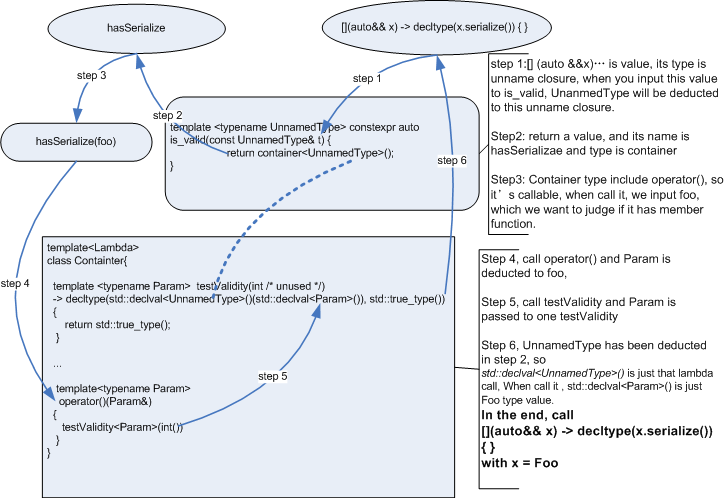
\includegraphics[scale=0.59]{pics/is_valid.png}
%\end{center}

	\item A better way in C++14/17 is to directly inherit from \texttt{std::true\_type}, which makes the source code simpler to read.

\begin{lstlisting}[frame=single, language=c++]
// Primary template, inherit from std::false_type.
template <typename T, typename = std::string>
struct hasSerialize : std::false_type { };

// Partial template specialisation, inherit from std::true_type.
template <typename T>
struct hasSerialize<T, decltype(std::declval<T>().serialize())> : std::true_type { };
\end{lstlisting}

	\item Building on previous technology, we also introduced \texttt{void\_t} in C++17, which makes it easier for us to define new type traits. For example, the code below judges whether the type \texttt{T} has a \texttt{reserve()} member function.
\begin{lstlisting}[frame=single, language=c++]
template <typename T, typename = void>
struct has_reserve : false_type {};

template <typename T>
struct has_reserve<T, void_t<decltype(declval<T&>().reserve(1U))>>: true_type {};
\end{lstlisting}

	\item There are two articles which are good.
"An introduction to C++'s SFINAE concept: compile-time introspection of a class member" and "checking expression validity in-place with C++17"
\end{itemize}
		
\subsubsection{ If T is function type? }

\begin{itemize}
	\item This is an example to test if T is function.
\begin{lstlisting}[frame=single, language=c++]
template <class T>
struct IsFunction{
	// int (*p)[1]  pointer to array(int [1])
	// int *p[1], that is array of pointer .
	template <typename C> 
	static constexpr bool test(C (*)[1] ){
		return false;
	}
	
	template <typename C> 
	static constexpr bool test(...){
		return true;
	}
	//use 0 as pretend pointer.
	static constexpr bool value = test<T>(0);
};

int f();
IsFunction<decltype(f)>::value; //value is true 
\end{lstlisting}
\begin{description}
	\item[Line 6:] Why we need declare a pointer to array? it will make line 14 easier, we can just use 0 as pretend pointer.
	\item[Source code:] There is three types you can't use to declare array, 1) void, 2) reference and 3) function type.  About function type, I will introduce below. 
\end{description}

\begin{enumerate}
	\item What is a function type?
\begin{lstlisting}
typedef int FT(); //FT is function type
typedef int (*PFT)(); //PFT is function pointer type

int f();  //f is variable
FT* fp= f;  //Usage of FT : fp is variable and type is function pointer

FT fv; 
void fv(){...} 
\end{lstlisting}
	\begin{description}

		\item[Line 7:] just like \texttt{int fv();} declare a function. How to define this variable make it linkable? Just like common function definition.
	\end{description}
	
	\item You can not define function type array.
\begin{lstlisting}
typedef int FT(); //FT is type
FT fa[3]; //compile error, error: declaration of 'fa' as array of functions
\end{lstlisting}

\end{enumerate}
\end{itemize}

\subsubsection{If T is member function type}
\begin{itemize}
	\item How to deal with member function pointer? Given an example code below, if you want to have member function pointer, its type should be: \texttt{int (A::*)() const \&} 
\begin{lstlisting}[frame=single, language=c++]
struct A {
	int fun() const&;
};
typedef int FunSignature() const&;
FunSignature A::*p = &A::fun;
\end{lstlisting}

	\item When we want to use template class to deduct it, it can be used in \texttt{U T::*}.
\begin{lstlisting}[frame=single, language=c++]
struct A {
	int fun() const&;
};

template<class T, class U>
struct PM_traits<U T::*> {
	using member_type = U;
};

int main() {
	using T = PM_traits<decltype(&A::fun)>::member_type; 
}
\end{lstlisting}

	\item Based on previous knowledge, we can implement 
\begin{lstlisting}[frame=single, language=c++]
template< class T >
struct is_member_function_pointer_helper : std::false_type {};

template< class T, class U>
struct is_member_function_pointer_helper<T U::*> :std::is_function<T> {};

template< class T >
struct is_member_function_pointer : is_member_function_pointer_helper<
                        std::remove_cv_t<T>  {};

class A {
public:
	void member() { }
};
//&A::member is expression, decltype change it to a type.
cout<<std::is_member_function_pointer<decltype(&A::member)>::value
\end{lstlisting}


\end{itemize}


\subsection{Applications of type trait}

\subsubsection{Tag dispatch}
\begin{itemize}
	\item There are \textbf{three} main usages of type traits:
\begin{enumerate}
	\item Correctness. 
\begin{lstlisting}
template<typename T>
T gcd(T a, T b) {
	static_assert(std::is_integral<T>::value, "T should be an integral type!");  // (1)
	if( b == 0 ){ return a; }
	else{
		return gcd(b, a % b);
	}
}	
\end{lstlisting}
	\item More generic. For a template functor, you can obtain the value type from \texttt{iterator\_traits} of the container. This information can be used in a template function object. The source code is very interesting because it combines the container, algorithm, and template function. It supports almost any generic type.
\begin{lstlisting}[frame=single, language=c++]
template<typename T>
struct Half{
	T operator()(T t){return t/2;}
};

vector vv(10, 6);
std::transform(begin(vv), end(vv),  begin(vv), Half< std::iterator_traits<decltype(begin(vv))>::value_type >{});		
\end{lstlisting}	

	\item Optimization. 
\begin{lstlisting}
template <typename I, typename T, bool b>
void fill_impl(I first, I last, const T& val, const std::integral_constant<bool, b>&){
	for(...)
}

template <typename T>                                                             
void fill_impl(T* first, T* last, const T& val, const std::true_type&){
	std::memset(first, val, last-first);
}

template <class I, class T>
inline void fill(I first, I last, const T& val){
	typedef std::integral_constant<bool,std::is_trivially_copy_assignable<T>::value> boolType;                                           
	fill_impl(first, last, val, boolType());
}
\end{lstlisting}
\end{enumerate}
	
	
	\item A famous usage of tag dispatch is in iterators. Pay attention to \texttt{iterator\_traits}. Why do we use it here? It's a template that, with specialization, can support common pointer types. The client side may or may not be a template. For \texttt{advance}, it should be a template because it needs a template parameter \texttt{InputIterator}. There are some tag types that need to be defined, and you should use these tags in the functions that you want to dispatch by overload resolution at compile time. 

\begin{lstlisting}[numbers=none]
struct input_iterator_tag { };
struct random_access_iterator_tag { };

template <class InputIterator, class Distance>
void advance_dispatch(InputIterator& i,Distance n,input_iterator_tag) {
	while (n--) ++i;
}
	
template <class RandomAccessIterator, class Distance>
void advance_dispatch(RandomAccessIterator& i,Distance n, random_access_iterator_tag) {
	i += n;
}

template <class InputIterator, class Distance>
void advance(InputIterator& i, Distance n) {
	typename iterator_traits<InputIterator>::iterator_category category;
	advance_dispatch(i, n, category);
}	
\end{lstlisting}	

    \item use \texttt{true\_type} or \texttt{flase\_type} in tag dispatch. The idea is just like previous iterator. Another interesting point is that overload function can return different types. foo's return type is \texttt{int} if it calls the \texttt{std::true\_type} overload and \texttt{double} if it calls the \texttt{std::false\_type} overload. So here we use \texttt{auto} as function return type. examples.
\begin{lstlisting}[numbers=none]
template <typename T>
int foo_impl(T value, std::true_type) {...}

template <typename T>
double foo_impl(T value, std::false_type) {...}

template <typename T>
auto foo(T value) {  //please note here, we use auto!
	return foo_impl(value, std::is_arithmetic<T>{});
}
\end{lstlisting}

\end{itemize}

\subsubsection{enable\_if}
\begin{itemize}
	
	\item For false, \texttt{enable\_if} is empty define.
\begin{lstlisting}[numbers=none]
template <bool, typename T = void>
struct enable_if {};

template <typename T>
struct enable_if<true, T> {
	typedef T type;
};	
\end{lstlisting}	

	\item When we make the call \texttt{do(25)}, the compiler selects the first overload: since the condition \texttt{std::is\_integral<int>} is true, the specialization of struct \texttt{enable\_if} for true is used, and its internal type is set to int. The second overload is omitted because without the true specialization (\texttt{std::is\_class<int>} is false) the general form of struct \texttt{enable\_if} is selected, and it doesn't have a type, so the type of the argument results in a substitution failure.

\begin{lstlisting}[numbers=none]
template <typename T>
void do(typename enable_if<std::is_integral<T>::value, T>::type &t){
	// an implementation for integral types 
}

template <typename T>
void do(typename enable_if<std::is_class<T>::value, T>::type &t) {
	// an implementation for class types
}		
\end{lstlisting}	
	
	\item Another example which use \texttt{enable\_if}. \texttt{has\_serialize} trait has been introduced in the type trait section, you can see the detail there. 
	
\begin{lstlisting}[numbers=none]
template <class T>
enable_if<has_serialize<T>::value, std::string>::type
serialize(const T& obj){
	return obj.serialize();
}

// Contra-SFINAE to avoid ambiguity
template <class T>
enable_if<!has_serialize<T>::value, std::string>::type 
serialize(const T& obj){
	return to_string(obj);
}	
\end{lstlisting}	
	
%	\item This technology has been used widely inside of vector.
%\begin{lstlisting}[frame=single, language=c++]
%template <typename T>
%class vector {
%	vector(size_type n, const T val);
%	
%	template <class InputIterator>
%	vector(InputIterator first, InputIterator last);
%	...
%}
%
%template <class _InputIterator>
%vector(_InputIterator __first,
%typename enable_if<__is_input_iterator<_InputIterator>::value &&
%!__is_forward_iterator<_InputIterator>::value &&
%... more conditions ...
%_InputIterator>::type __last);
%\end{lstlisting}	

	
	\item An example of usage of \texttt{enable\_if}. We can also use \texttt{enable\_if} to "delete" a function for certain type. 
\begin{lstlisting}
template<typename T>
class MyClass{
	public:
	void f(T const&  x){}
	
	template<typename T_ = T, typename=std::enable_if_t<!std::is_reference_v<T_> >>
	void f(T&& x){}  //T can't be reference 
};	
\end{lstlisting}
\begin{description}
	\item[Line 6:] Pay more attention to five points here: 
	1) unname template parameter. There is no name after second typename. 
	2) \texttt{enable\_if\_t} is alias template.
	3) \texttt{is\_reference\_v} is variable template. 
	4) Why do we need \texttt{T\_}? f must be a template function, although it's inside another template class. These two template need to use different template parameter. 
	5) \texttt{enable\_if} should be used in template parameter deduction first; don't use it for function parameters or function return types unless you have a strong reason.
\end{description}

	\item A common pattern to select a function according to input type.
\begin{lstlisting}
template<typename T,
std::enable_if_t<std::is_same<int, T>::value>* = nullptr>
void f() { }

template<typename T,
std::enable_if_t<std::is_same<double, T>::value>* = nullptr>
void f() { }
//-----------------------------
template<typename T,
typename = std::enable_if_t<std::is_same<int, T>::value>>
void g() { }

template<typename T,
typename = std::enable_if_t<std::is_same<double, T>::value>>
void g() { }
\end{lstlisting}

	\item The usage of \texttt{std::enable\_if} is very flexible, it can be used 1) template function parameter, 2) template function return, 3) as a template parameter in one template function to suppress it, 4) as a template parater in two template functions to overload it. 

	\item In C++17, we can also use \texttt{if constexpr}, that make our code looks clean and simple. But the basic idea is the same. If your compiler support \texttt{if constexpr} or \texttt{concept}, please use it instead of \texttt{std::enable\_if}. I am afraid that this will be deprecated in the future version of C++ standard. 

\begin{lstlisting}[numbers=none]
template <typename T>
auto get_value(T t){
	if constexpr (std::is_pointer_v<T>) {
		return *t;
	} else {
		return t;
	}
}	
\end{lstlisting}

	\item A good article is "SFINAE and enable\_if"
\end{itemize}

\subsubsection{A practical example}
\begin{itemize}
    \item If we want to add some items to a kind of "container". We need to check if a container has reserve method(for example, vector). If we have this method, use it to reserve space before we use push back. Otherwise, we use push back directly. Below code build a type trait, it uses void\_t and true\_type. We have introduced before. 
\begin{lstlisting}
template <typename T, typename = void_t<>>
struct has_reserve : false_type {};
   
template <typename T>
struct has_reserve<T, void_t<decltype(declval<T&>().reserve(1U))>> : true_type {};   
\end{lstlisting}

    \item use tag dispatch to get static dynamic.
\begin{lstlisting}
template <typename C, typename T>
void _append(C& container, T* ptr, size_t size, true_type) {
    container.reserve(container.size() + size);
    for (size_t i = 0; i < size; ++i){ 
        container.push_back(ptr[i]);
    }
}

template <typename C, typename T>
void _append(C& container, T* ptr, size_t size, false_type){
    for (size_t i = 0; i < size; ++i) {
        container.push_back(ptr[i]);
    }
}

template <typename C, typename T>
void append(C& container, T* ptr, size_t size) { 
    _append(container, ptr, size, has_reserve<C>{}); 
}
\end{lstlisting}

%    \item You can use \texttt{enable\_if} too. The syntax is little "bloat" compared with \texttt{true\_type} dispatch. But one advantage of \texttt{enable\_if} is that you can use it not only in dispatch to two different implementations, but also filter a valid type to generate valid code, for invalid type, if you don't provide \texttt{!has\_reserve<C>} match, it will generate compiling error directly.
%\begin{lstlisting}
%template <typename C, typename T>
%enable_if_t<has_reserve<C>::value> append(C& container, T* ptr, size_t size){
%    container.reserve(container.size() + size);
%    for (size_t i = 0; i < size; ++i) {
%    	container.push_back(ptr[i]);
%    }
%}
%
%template <typename C, typename T>
%enable_if_t<!has_reserve<C>::value> append(C& container, T* ptr, size_t size){
%	for (size_t i = 0; i < size;  ++i) {
%        container.push_back(ptr[i]); 
%    }
%}
%\end{lstlisting}
%
	\item If you don't want to "dispatch", just want to use one function if it match.  When the input type is not valid, you hope to have compile error. Under such context, you can use decltype and declval directly.

\begin{lstlisting}[numbers=none]
template <typename C, typename T>
auto append(C& container, T* ptr, size_t size)-> 
              =decltype( declval<C&>().reserve(1U), void()){
	container.reserve( container.size() + size);
	for (size_t i = 0; i < size; ++i) {
		container.push_back(ptr[i]);
	}
}
\end{lstlisting}

\item use \texttt{if constexpr}
\begin{lstlisting}
template <typename C, typename T>
void append(C& container, T* ptr, size_t size){
    if constexpr (has_reserve<C>::value) {
        container.reserve(container.size() + size);
    }
    for (size_t i = 0; i < size; ++i) {
        container.push_back(ptr[i]);
    }
}   
\end{lstlisting}

	\item In C++ 20, we can use concept directly.  You can see that we use \texttt{HasReserve} here directly. The whole code is very clear, That is why we call concept as "future of generic programming" 
\begin{lstlisting}
template<typename T>
concept HasReserve = requires(T a){
    a.reserve();
};

template <HasReserve C, typename T>
void append(C& container, T* ptr, size_t size){
    container.reserve(container.size() + size);
    for (size_t i = 0; i < size; ++i) {
        container.push_back(ptr[i]);
    }
} 
\end{lstlisting}

\end{itemize}

\subsection{Type traits Summary}


\begin{itemize}
	\item Common type traits implementation methods includes
	\begin{enumerate}
		\item template partial specification: \texttt{is\_integer}
		\item use basic trait to build more complex one: \texttt{is\_swap}
		\item use template parameter deduction : \texttt{std::is\_function} and
		\texttt{is\_member\_function}, \texttt{is\_array}, \texttt{is\_class(T::*)}
		\item define trait in existing class : \texttt{iterator\_trait}.
		\item template class partial specification, with help of \texttt{decltype}, \texttt{declval} and void\texttt{\_t}. A good example is \texttt{has\_serialize}.	
	\end{enumerate}
	
	\item Use a few ways to implement type traits, then use these type traits to achieve static polymorphism and increase efficiency. This is the basic idea of generic programming.
\begin{center}
	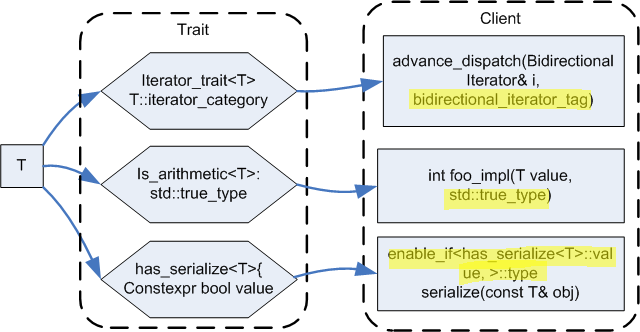
\includegraphics[scale=0.9]{pics/tag_dispatch.png}
\end{center}

%	\item For type\_trait side, we introduced two main methods. In "SFINAE(Type deduct) to build trait" section, we use these two methods to implement \texttt{hasSerialize}. After C++ 14, we recommend to use \texttt{void\_t} method. But after C++ 20, we strongly recommend to use \textbf{concept}. On the other side, as a client, we mainly use \texttt{enable\_if} and tag dispatch. But after C++17, we strongly recommend use \texttt{if constexpr} and concept. In one word, if you compiler supports concept, use it to define type trait and use it in the client code too. 
	
	 \item With the development of C++, we have had three major generations of technology for defining and using types in template metaprogramming.
	
	\begin{tabular}{|p{0.14\textwidth} |p{0.38\textwidth}|p{0.38\textwidth}|}
		\hline
		C++ version & build type trait method  & use type trait method \\
		\hline
		C++11& static and size of & enable\_if \\
		\hline
		C++14/17& \specialcell[t]{1) void\_t, true\_type \\  
			                      2) decltype and constexpr \\
		                          3) hasSerialize is example} & \specialcell[t]{1) constexpr\ if \\ 2)true\_type overload } \\
		\hline
		C++2x & requires expression & requires clause \\
		\hline
	\end{tabular}

	We should use the new generation technology if the compiler supports it, because it's easier to write and maintain. The requires expression and requires clause will be introduced in the Modern C++ chapter. You can see how elegant the requires expression is when we want to check if T has a certain member function.
\begin{lstlisting}
template <typename T>
concept HasSquare = requires (T t) {
	{t.square()} -> std::convertible_to<int>;
}; 	
\end{lstlisting}	
	
\end{itemize}


\section{template common idiom}

\subsection{policy, mixin and CRTP}
These three patterns are associated, so I put them together. 

\subsubsection{policy}
\begin{itemize}
	
	\item The Policy class can be thought of as an optional of multiple inheritance. Why do we use private inheritance here? Because we don't want to expose \texttt{print} and \texttt{message} methods. We just want to use it. So we use private inheritance here.
	
\begin{lstlisting}[numbers=none]
class OutputPolicyWriteToCout{
	protected:
	template<typename MessageType>
	void print(MessageType const &message) const{
		std::cout << message << std::endl;
	}
};

class LanguagePolicyEnglish{
	protected:
	std::string message() const{
		return "Hello, World!";
	}
};

class LanguagePolicyGerman{
	protected:
	std::string message() const{
		return "Hallo Welt!";
	}
};

template <typename OutputPolicy, typename LanguagePolicy>
class HelloWorld : private OutputPolicy, private LanguagePolicy{
public:
	void run() const{
		print(message()); // Two policy methods
	}
};
\end{lstlisting}


	\item With previous class definition, client code looks like below:
\begin{lstlisting}[numbers=none]
typedef HelloWorld<OutputPolicyWriteToCout, 
           LanguagePolicyEnglish> HelloWorldEnglish;
HelloWorldEnglish hello_world;
hello_world.run(); // prints "Hello, World!"


typedef HelloWorld<OutputPolicyWriteToCout,LanguagePolicyGerman> HelloWorldGerman;
HelloWorldGerman hello_world2; 
hello_world2.run(); // prints "Hallo Welt!"
\end{lstlisting}
	
	\item If polymorphism can be determined at compile time, we can use 'static polymorphism' by injecting a class with static methods using template parameters. These methods can be inlined and will incur no runtime overhead.
	
\begin{lstlisting}[frame=single, language=c++]
// char_traits::eq, traits with case-insensitive eq:
struct custom_traits: std::char_traits<char> {
	static bool eq (char c, char d) { 
	return std::tolower(c)==std::tolower(d); 
}
	
static const char* find (const char* s, std::size_t n, char c)
	{ while( n-- && (!eq(*s,c)) ) ++s; return s; } // call your eq here
};
	
std::basic_string<char,custom_traits> str ("Test");
std::cout<< "found at position" <<str.find('t') ;
\end{lstlisting}

	
	\item This kind of example can be found frequently in the STL, often implemented using a functor. The basic idea remains the same. All of these technologies are part of generic programming. A good example of this is found in the book "Modern C++ Design", where the first chapter introduces the policy pattern and the second chapter introduces several techniques for managing type information at compile time. 
	
\end{itemize}

\subsubsection{Mixin}
\begin{itemize}
	
	\item How can we understand Mixin? At a semantic level, it's the idea of adding new code (new functions) to an existing class. At a syntactic level, there are different ways to achieve this goal. For example, the following three different approaches are all considered "Mixin", and each has its own unique application scenarios.
	\begin{enumerate}
		\item Method 1 involves creating a base (Mixin) class that includes the regular \texttt{operator new}, and then having your own existing class inherit from it. This method is introduced in the "Memory" chapter's "Operator new overload" section. For this scenario, the Mixin class doesn't depend on the existing class; it simply adds some common functions.	
		
		\item Method 2 involves using CRTP, such as \texttt{enable\_from\_this}. The main point here is that CRTP will generate a new base class, which is different due to the different child class. Let me explain this in detail. In the next section, "CRTP", we provide an example of how to calculate the number of objects that have been generated. The CRTP pattern works for this example, but method 1 doesn't work. The same idea also applies to \texttt{enable\_from\_this}, as they require different \texttt{weak\_ptr} points for different classes.
		
		\item Method 3 is an template class, which is parameterized on its base class. Such as RepeatPrint which I will introduce next.
	\end{enumerate}
	In one word, please understand Mixin in semantic way, not in syntax way.
	
	\item Method 3 involves using template classes that define generic behavior and are designed to inherit from the type you wish to plug their functionality onto. For example, RepeatPrint is a Mixin class, where T is the type you wish to plug the functionality onto.
	
\begin{lstlisting}[numbers=none]
template<typename T>
class RepeatPrint : T{
	explicit RepeatPrint(T const& printable) : T(printable) {}
	void repeat(unsigned int n) const{
		while (n-- > 0){
			this->print(); //Make sure printable has print method
		}
	}
};
\end{lstlisting}
	
	\item Supposing that we have an existing type which has a print method.
\begin{lstlisting}[numbers=none]
class Name{
public:
	Name(std::string firstName, std::string lastName)
	: firstName_(std::move(firstName)), lastName_(std::move(lastName)) {}
	
	void print() const{
		std::cout << lastName_ << ", " << firstName_ << '\n';
	}
private:
	std::string firstName_, lastname;
};
\end{lstlisting}
	
	\item Client side can use \texttt{RepeatPrint} class by two ways:
\begin{lstlisting}[numbers=none]
template<typename T> //method 1, we use object generator pattern
RepeatPrint<T> rpGen(T const& printable){
	return RepeatPrint<T>(printable);
}
Name ned{"Eddard", "Stark"};    
rpGen(ned).repeat(10);

RepeatPrint<Name> rp{"Eddard", "Stark"}; \\method 2, specify type explicitly
rp.repeat(10)
\end{lstlisting}

\end{itemize}


\subsubsection{CRTP}
\begin{itemize}
	\item The basic syntax is Templates Parameterised by a Derived Class.
	
\begin{lstlisting}[numbers=none]
template <class T> 
struct Base{
	void interface(){
		static_cast<T*>(this)->implementation();
		// ...
	}
	
	static void static_func(){
		T::static_sub_func();
		// ...
	}
};
	
struct Derived : Base<Derived>{ //That is CRTP
	void implementation();
	static void static_sub_func();
};
\end{lstlisting}
	
	
	\item There are two common usages from CRTP:
	\begin{enumerate}
		\item Static polymorphism avoids the cost of runtime polymorphism. An easy way to implement a 'callback' is through a function pointer, but it cannot be used inline, resulting in an efficiency problem. Another option is to use inheritance, which involves runtime polymorphism and has some associated overhead.
\begin{lstlisting}[numbers=none]
template<typename specific_animal>
struct animal {
	void speak() { static_cast<specific_animal*>(this)->speak(); }
};
struct dog : animal<dog> {
	void speak() { cout << "bark!" << endl; }
};
struct cat : animal<cat> {
	void speak() { cout << "miao!" << endl; }
};
template<typename specific_animal>
void speakFun(animal<specific_animal> &animal) {
	animal.speak();
}
cat c;
speakFun(c); // output bark
dog d;
speakFun(d); // output miao
\end{lstlisting}

\item Adding functionality to existing class, that is a kind of "Mixin". The code below calculates the number of objects that have been generated.

\begin{lstlisting}[]
template <typename T>
struct counter{
	static int objects_created;
	counter(){ ++objects_created;}
};
template <typename T> 
int counter<T>::objects_created{0}; //initializing statement.

class X : counter<X>{
	// ...
};

X x;
cout<<X::objects_created<<endl;
\end{lstlisting}

	\end{enumerate}

	\item Below is another example of a template class that uses CRTP. In the source code below, the class \texttt{yan\_vect} is a template class. In comparison with class \texttt{X} from the previous source code, the previous example is a non-template class.
\begin{lstlisting}
template<typename T>
class Base{
public:
	int DoubleSum(){
		return static_cast <T &>(*this).sum()*2;
	}    
};

template<typename T>
struct yan_vect :public Base<yan_vect<T> >{
	yan_vect(int num, T v){...}
	T sum(){
		T result{};
		for (int i = 0 ;i<num_; i++)
			result += a[i];
		return result;
	}
T a[10];
int num_;
};

template<typename T>
void fun(Base<T>& bt){
	cout<<bt.DoubleSum()<<endl;
}

int main(){
	yan_vect<int> vi = {5,2};
	yan_vect<float> vf = {5,1.2};
	fun(vi);
	fun(vf);
}
\end{lstlisting}

%	\item CRTP pattern with template template class, you can see the \texttt{class Base} has template template argument. The below is syntax demo. This pattern doesn't use very widely, I just found on practical usage. please google "An Implementation Helper For The Curiously Recurring Template Pattern"

%\begin{lstlisting}
%template<typename T, template< typename > class child>
%class Base{
%	public:
%	int DoubleSum(){
%		return static_cast <child<T> &>(*this).sum()*2;
%	}    
%};
%
%template<typename T>
%struct yan_vect :public Base<T, yan_vect>{
%	yan_vect(int num, T v){...}
%	T sum(){
%		T result{};
%		for (int i = 0 ;i<num_; i++)
%			result += a[i];
%		return result;
%	}
%T a[10];
%int num_;
%};
%
%template<typename T >
%void fun(Base<T, yan_vect >& bt){
%	cout<<bt.DoubleSum()<<endl;
%}
%
%int main(){
%	yan_vect<int> vi = {5,2};
%	yan_vect<float> vf = {5,1.2};
%	fun(vi);
%	fun(vf);
%}
%\end{lstlisting}

	\item Another interesting example is CRTP on CRTP. How to understand below code? \texttt{Scale} add functionality to \texttt{Sensitivity}, \texttt{crtp} add functionality to \texttt{Scale} and \texttt{Square}.
\begin{lstlisting}
template <typename T, template<typename> class crtpType>
struct crtp{
	T& underlying() { return static_cast<T&>(*this); }
	T const& underlying() const { return static_cast<T const&>(*this); }
private:
	crtp(){}
	friend crtpType<T>;
};

template <typename T>
struct Scale : crtp<T, Scale>{
	void scale(double multiplicator){
		this->underlying().setValue(this->underlying().getValue() * multiplicator);
	}
};
template <typename T>
struct Square : crtp<T, Square>{
	void square(){
		this->underlying().setValue(this->underlying().getValue() * this->underlying().getValue());
	}
};

class Sensitivity : public Scale<Sensitivity>, public Square<Sensitivity>{
	public:
	double getValue() const { return value_; }
	void setValue(double value) { value_ = value; }	
private:
	double value_{3.3};
};

Sensitivity s;
s.scale(2);
cout<<s.getValue()<<endl;  //output 6.6 here. 
\end{lstlisting}

	\item For CRTP: 1) impacts the definition of the existing class, because it has to inherit from the CRTP; 2) client code uses the original class directly and benefits from its augmented functionalities.

	\item For Mixin class, 1) leaves the original class unchanged. 2) client code doesn’t use the original class directly, it needs to wrap it into the mixin to use the augmented functionality. 3) inherits from a the original class even if it doesn’t have a virtual destructor. This is ok unless the Mixin class is deleted polymorphically through a pointer to the original class.

\end{itemize}

\subsubsection{meta-programming}
\begin{itemize}


\item basic component.
\begin{enumerate}
	\item enum static, constexpr constant in compiling time
	\item typedef and using to define meta data.
	\item template, you can think that is "meta function" all the logic are calculated inside it when the compiler analyze the template.  It's core idea in meta-programming.
	\item ::
	\item please see a good example below. 
\begin{lstlisting}
	template<int N, int M>
	struct meta_func{
		static constexpr int value = N+M;
	}
	
	cout<<meta_func<10, 20>::value. 
\end{lstlisting}
	
\end{enumerate}
	\item branch, based on template specification
\begin{lstlisting}
template<bool B>
class IfElse{};

template<bool true>
class IfElse{
	static inline void func(){
		cout<<"output true";
	}
};

template<bool false>
class IfElse{
	static inline void func(){
		cout<<"output false";
	}
};

IfElse<(2+3 ==6)>::func(); //usage. 
\end{lstlisting}
	\item loop, based on recursive. 
\begin{lstlisting}
template<int Number>
struct Fibo{
	enum{
		value = Fibo<Number-1>::value+Fibo<Number-2>::value
	};
};

template<>
struct Fibo<0>{
	enum{
		value = 0
	};
};

template<>
struct Fibo<1>{
	enum{
		value = 1
	};
};
\end{lstlisting}
	

\end{itemize}


\subsubsection{A practical example}
\begin{itemize}
	\item Consider the Task Manager framework, which requires certain functionalities to be shared among task implementations. For instance, task execution timing and logging of start and completion messages are two common features. In this context, we have explored six different approaches to implementing these features.
	
	\item method 1, use Mixin
	\begin{enumerate}
		
		\item The function name (Execute) can be different. Here, we use the same name because we can recursive use it. such as: \texttt{LoggingTask< TimingTask< MyTask > > Task;}
		
		\item A detail can be found "C++ Mixins - Reuse through inheritance is good... when done the right way" and "Mixin Classes: The Yang of the CRTP"
		
\begin{lstlisting}[numbers=none]
struct MyTask{
void Execute(){
		std::cout << "task is executed" << std::endl;
	}
};
		
template<typename T >
class LoggingTask : public T{
public:
	explicit LoggingTask(T const& t) : T(t) {}
			
	void Execute(){
		std::cout << "LOG: The task is starting - " ;
		T::Execute(); 
		std::cout << "LOG: The task has completed - " ;
	}
};
		
LoggingTask< MyTask > task;
task.Execute();
\end{lstlisting}
		
		\item if you have a \texttt{MyTask} variable, you can build a helper function to build Mixin class 
\begin{lstlisting}[numbers=none]
template<typename Task>
LogTask<Task> getLogTask(Task const& task){
	//Call the below explicit constructor in LogTask class
	return LogTask<Task>(task);
}
		
getLogTask(task).Execute //with log functions
\end{lstlisting}
		
	\end{enumerate}
	
	\item method 2, use CRTP. Use base class extend and reuse function(Execute\_imp). Expose Execute interface to client by base class. Client can directly use MyTask.
	
\begin{lstlisting}[numbers=none]
template< class Task >
class LoggingTask {
public:
	void Execute(){
		std::cout << "LOG: The task is starting - " ;
		static_cast<Task const&>(*this).Execute_imp();
		std::cout << "LOG: The task has completed - " ;
	}
};
	
class MyTask:public LoggingTask<MyTask> {
public:
	void Execute_imp(){
		std::cout << ".task is executed..." ;
	}
};
	
MyTask task;
task.Execute();
\end{lstlisting}
	
	\item method 3, template Method. No template, just use run time polymorphism. Base class define a basic flow of action, some part of action is override in the Child class, That is Template Method pattern in design pattern.

\begin{lstlisting}[numbers=none]
class BaseLoggingTask{
public:
	void Execute(){
		std::cout << "LOG: The task is starting - " ;
		OnExecute();
		std::cout << "LOG: The task has completed - ";
	}
	virtual void OnExecute() = 0;
};
	
// Concrete Task implementation that reuses the logging code of the BaseLoggingTask
class MyTask : public BaseLoggingTask{
public:
	virtual void OnExecute(){
		std::cout << "task is executed..." << std::endl;
	}
};
	\end{lstlisting}
	
	\item method 4, command pattern. For Logging Task, you can see the class \textbf{includes and derived from ITask at the same time}. 

\begin{lstlisting}[numbers=none]
class LoggingTask : public ITask{
	ITask* task_;
public:
	LoggingTask( ITask* task ) : task_( task ){ }
	
	~LoggingTask(){
	delete task_;
}
	
	virtual void Execute(){
		std::cout << "LOG: The task is starting - " 
		          << GetName().c_str() << std::endl;
		if( task_ ) task_->Execute();
		std::cout << "LOG: The task has completed - " 
		         << GetName().c_str() << std::endl;
	}
};
	
class MyTask : public ITask{
public:
	virtual void Execute(){
		std::cout << ".task is executed..." ;
	}
};
	
ITask* t = new LoggingTask(new MyTask()) ;
t->Execute();
\end{lstlisting}
	
	\begin{center}
		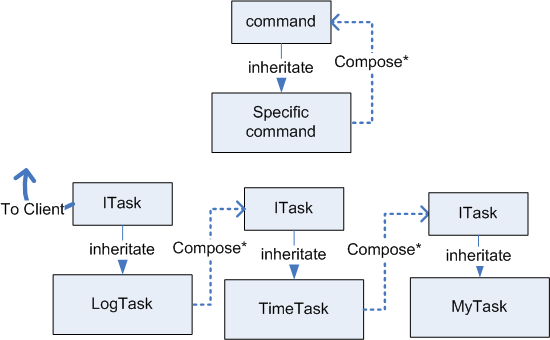
\includegraphics[scale=0.9]{pics/command.png}
	\end{center}
	
	
	\item method 5, mixin many mixin

\begin{lstlisting}[numbers=none]
template< class T >
class LoggingTask : public T{
	public:
	void Execute(){
		std::cout << "LOG: The task is starting - " 
		         << GetName().c_str() << std::endl;
		T::Execute();
		std::cout << "LOG: The task has completed - " 
		         << GetName().c_str() << std::endl;
	}
};
	
template< class T >
class TimingTask : public T{
	Timer timer_;
public:
	void Execute(){
		timer_.Reset();
		T::Execute();
		double t = timer_.GetElapsedTimeSecs();
		std::cout << "Task Duration: " << t <<;
	}
};
	
class MyTask{
	public:
	void Execute(){
		std::cout << "task is executed..." ;
	}
};
	
tyedef LoggingTask< TimingTask< MyTask > > Task;
Task t4;
t4.Execute();
\end{lstlisting}

		\item method 6, policy base
\begin{lstlisting}[numbers=none]
class coutLog{
	void beginLog(){
		cout<< "LOG: The task is starting - " <<endl
	}
	
	void endLog(){
		cout << "LOG: The task has completed - "
	}
}
	
template<typename LogPolicy, typename TimePolicy>
class Task: private LogPolicy, TimePolicy{
	void Execute(){
		beginLog();
		beginTime();
		std::cout << "This is where the task is executed";
		endTime();
		endLog();}
\end{lstlisting}
	
	\item Comparison of above methods.
	\begin{enumerate}
		\item Policy pattern can be useful when there are frequent changes in log and time function.
		\item Both Mixin and command can be combined to itself to perform multiple actions.
		\item template is more efficient than inheritance. 
		\item Command pattern has similar structure to the the composite pattern.
		\item Mixin do not modify the current class, while CRTP changes the interface of current class.
	\end{enumerate}
	
\end{itemize}

\subsubsection{summary}
\begin{itemize}
	\item The basic idea is illustrated below in this important figure, which is worth exploring to gain a deeper understanding. For example, if we consider the class \texttt{Foo: T}, we can refer to it as the policy idiom if we focus on \texttt{Foo}, or as the mixin idiom if we focus on \texttt{T}. In the mixin idiom, \texttt{Foo} is only intended to add some functionality to \texttt{T}. CRTP follows the same idea, where we use static polymorphism when focusing on the parent class, and add functionality to the child class when focusing on it. A common use case for this idea is with \texttt{std::enable\_shared\_from\_this}.

		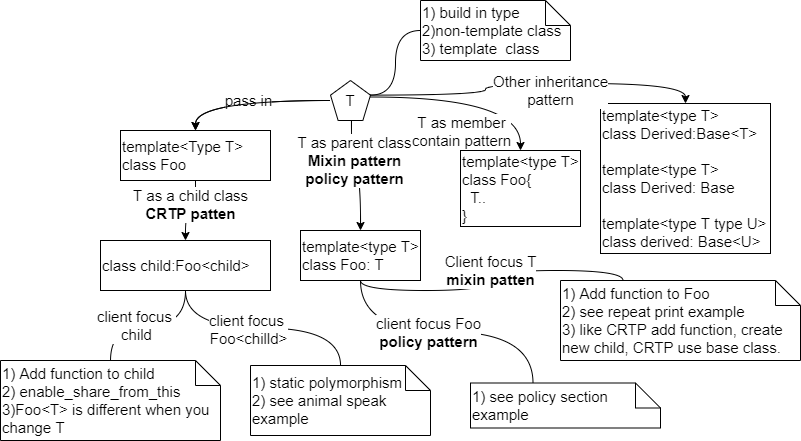
\includegraphics[width=0.9\linewidth]{pics/template1.drawio.png}
		
	\item For Contain pattern, we can use template template parameter. A good example is using a container to implement stack code in  "common used template technologies" section.
	
		%\includegraphics[width=0.9\linewidth]{pics/mixin_tt.png}
		\includegraphics[width=0.9\linewidth]{pics/template2.drawio.png}
		
	\item For CRTP pattern, there are two advanced usage. 1)we can use template class as child class, an example is \texttt{yan\_vect} code in CRTP section.  2)we can use template template parameter too. A goog example is adding scale and square to sensitivity code in CRTP section. 
	
		%\includegraphics[width=0.9\linewidth]{pics/crtp_tt.png}
		\includegraphics[width=0.9\linewidth]{pics/template3.drawio.png}

\end{itemize}


\subsection{type erasure and concept}


\begin{itemize}
	
	\item Most compilers treat all member function pointers identically, regardless of the class. For most of them, a straightforward \texttt{reinterpret\_cast<>} from the given member function pointer to the another member function pointer would work. This technology is used widely as a kind of member function type erasure method. The detail can be found in this link:
	
	https://www.codeproject.com/Articles/7150/Member-Function-Pointers-and-the-Fastest-Possible
\begin{lstlisting}
class A{
	public:
	int f(){cout<<"222"<<endl;; return 0;}
};

class B{
};

typedef int (B::*PMB)();
typedef int (A::*PMA)();	
PMA pma = &A::f;
A a;

B* pb = reinterpret_cast<B*>(&a); //to an unrelated class.
PMB pmb =(PMB)(pma); //to an unrelated member function pointer.
(pb->*pmb)();
\end{lstlisting}
		
	\item When you implement type erasure, it always starts with making a list of the things you want to be able to do with your type-erased object - call it, destroy it, copy it, and so on. For example, A \texttt{std::function} affords copying and calling. A \texttt{std::any} affords copying, but not calling. A \texttt{std::move\_only\_function} affords calling and moving, but not copying.

	
	\item Each item in your requirement list becomes a virtual member function of \texttt{AbstractWhatever}, which will then be appropriately overridden by \texttt{WrappingWhatever<T>} for T. At the top-level, \texttt{Whatever} stores a \texttt{unique\_ptr<AbstractWhatever> ptr\_} (and/or an SBO buffer) and provides a clean non-virtual interface that is implemented entirely by calling virtual member functions on \texttt{*ptr\_}. An example implementation is illustrated in the code and picture below.

\begin{center}
	\includegraphics[scale=0.9]{pics/function1.png}
\end{center}

\begin{lstlisting}[frame=single, language=c++]
struct Plus1 {
	int call(int x) const { return x+1; }
};
struct AbstractCallback {
	virtual int call(int) const = 0;
	virtual ~AbstractCallback() = default;
};
template<class T>
struct WrappingCallback : AbstractCallback {
	T cb_;
	explicit WrappingCallback(T &&cb) : cb_(std::move(cb)) {}	                
	int call(int x) const override  { return cb_(x); }
};
struct Callback {
	std::unique_ptr<AbstractCallback> ptr_;
	template<class T>
	Callback(T t) {
		ptr_ = std::make_unique<WrappingCallback<T>>(std::move(t));
	}
	int operator()(int x) const { return ptr_->call(x);}
};

int run_twice(const Callback& callback) {
	return callback(1) + callback(1);
}
int y = run_twice([](int x) { return x+1; });
assert(y == 4);
\end{lstlisting}

	\item A good article is "What is Type Erasure" A detail implementation can be found in:\\ \verb|http://blog.bitfoc.us/p/525|
	 
\end{itemize}



\chapter{STL}
\section{Four components and design idioms in STL}
\begin{itemize}
	\item The main principle of design of STL library is: Use \textbf{functors} to customize \textbf{algorithms}, and then apply the algorithm on \textbf{containers} using \textbf{iterators}. For example, algorithms such as \texttt{std::for\_each} take two iterators as input and do not care about the container they operate on. 
\begin{lstlisting}[frame=single, language=c++]
struct Sum{ //functors are usually struct, not class
	Sum(): sum{0} { }
	void operator()(int n) { sum += n; }
	int sum;
};

std::vector<int> nums_v{3, 4, 2, 8, 15, 267};
std::list<int> nums_l{3, 4, 2, 8, 15, 267};
std::for_each(nums_v.begin(), nums_v.end(), [](int &n){ n++; }) //lambda syntax
Sum s = std::for_each(nums_l.begin(), nums_l.end(), Sum());  //return Sum struct
cout<<s.sum<<endl;	
\end{lstlisting}	
	
	\item When using the STL library, it is important to always include the proper headers. Specifically, you should include the corresponding header files when using containers and algorithms.
\begin{enumerate}

	\item All the algorithms are declared in <algorithm>. \texttt{std::inner\_product}, \\ \texttt{std::adjacent\_difference}, \texttt{std::partial\_sum} and \texttt{std::accumulate} are in the <numeric>.

	\item Special kinds of iterators, including \texttt{std::istream\_iterators}, are found in the <iterator> library.

	\item Standard functors, such as \texttt{less<T>} and functor adapters like \texttt{not1} and \texttt{bind2nd}, are declared in \texttt{<functional>}. However, it is not recommended to use these functor adapters in C++11 because C++11 introduced the \texttt{function} and \texttt{bind} templates.

	\item For most of time, you need \texttt{algorithm, numeric, range, iostream, format, iterator , functional, utility} eight header files, besides the corresponding container header file. If you need template metaprogramming, you should also includes \texttt{type\_traits, concepts}.  
\end{enumerate}

	\item Below are some commonly used idioms in STL:
1) concept,
2) type traits, 
3) tag dispatching,
4) adapters,
5) type generators,
6) object generators,
7) policy classes.

	\item Concept is a set of requirements consisting of valid expressions, associated types, invariant, and complexity guarantees. A type that satisfies the requirements is said to \textbf{model} the concept. A concept can extend the requirements of another concept, which is called \textbf{refinement}.
	\begin{enumerate}
		\item Valid expressions are C++ expressions which must compile successfully for the objects involved in the expression to be considered models of the concept. For example, an \texttt{Iterator x} is expected to support the expressions \texttt{++x} and \texttt{*x}.
		
		\item Associated types are types that are related to the modeling type in that they participate in one or more of the valid expressions. Typically associated types can be accessed either through typedefs nested within a class definition for the modeling type, or they are accessed through a traits class. For example, an iterator's value type is associated with the iterator through \texttt{std::iterator\_traits}
\begin{lstlisting}
template<class BidirIt>
void my_reverse(BidirIt first, BidirIt last){
	typename std::iterator_traits<BidirIt>::difference_type n = std::distance(first, last);
	for (--n; n > 0; n -= 2){
		typename std::iterator_traits<BidirIt>::value_type tmp = *first;
		*first++ = *--last; *last = tmp;
	}
}
std::vector<int> v{1, 2, 3, 4, 5};  //int type behind iterator
my_reverse(v.begin(), v.end());
std::list<float> v{1, 2, 3, 4, 5};  //float type behind iterator
my_reverse(v.begin(), v.end());
\end{lstlisting}
		
		\item Invariants are run-time characteristics of the objects that must always be true, that is, the functions involving the objects must preserve these characteristics. The invariants often take the form of pre-conditions and post-conditions. For example, forward iterator is copied, the copy and original must compare equal.
		
		\item Complexity Guarantees are maximum limits on how long the execution of one of the valid expressions will take, or how much of various resources its computation will use.
	\end{enumerate}

	\item A type generator is a template whose only purpose is to synthesize a new type or types based on its template argument(s). The generated type is usually expressed as a nested typedef named, appropriately type. Another good example of type generator is \texttt{std::integral\_constant}.
\begin{lstlisting}[numbers=none]
template <typename Value>
struct Directory{
	typedef std::map <std::string, Value, std::less<std::string>, 
	__gnu_cxx::malloc_allocator<std::string> > type;
};

Directory<int>::type var_d1;   // gives a map of string to integers.

//Better method in C++11, use alias template
template <typename Value> 
using Directory = std::map <std::string, Value, std::less<std::string>, 
	__gnu_cxx::malloc_allocator<std::string> > ;
	
Directory<int> var_d1;
\end{lstlisting} 
	
	\item An object generator is a function template whose only purpose is to construct a new object out of its arguments. Think of it as a kind of \textbf{generic constructor}. An object generator may be more useful than a plain constructor when the exact type to be generated is difficult or impossible to express and the result of the generator can be passed directly to a function rather than stored in a variable. Most Boost object generators are named with the prefix "make\_", after \texttt{std::make\_pair(const T\&, const U\&)}.
	
	\item An adapter is a class template which builds on another type or types to provide a new interface or behavioral variant. Examples of standard adapters are \texttt{std::reverse\_iterator}, which adapts an iterator type by reversing its motion upon increment/decrement, and \texttt{std::stack} , which adapts a container to provide a simple stack interface.
	
\end{itemize}


\section{Container}

\subsection{Basic knowledge}
\begin{itemize}

	\item Anytime you want to write \texttt{new [..]} just for allocate dynamic array, using a \texttt{std::vector} or \texttt{std::string} instead, and using \texttt{reserve()} to allocate enough space for large amount of data for memory efficiency.
		
	\item For all containers in the STL, the general principle is "Copy in, Copy out." However, in C++11, you can utilize the \texttt{emplace\_back}, \texttt{emplace} or \texttt{try\_emplace} member function to directly construct objects within a container to avoid unnecessary copying.
\begin{lstlisting}[numbers=none]
int j = 10;
vector<int> vc;
vc.push_back(j); // not j, but copy of j to vc

int i = vc.pop_back(); 
i = -99 // when you modify i, not effect on vc
\end{lstlisting}

	\item Even for copy-in, copy-out operations, \texttt{std::vector} is more flexible than arrays in C language because it uses heap memory. If you want to use stack memory instead, you can use \texttt{std::array}.
\begin{lstlisting}[numbers=none]
Foo farray[50]; //default constructor has been called 50 times.
Foo *parray = new Foo[50]; //Same, constructor will be called 50 times.

vector<Foo> fvc; // NO default constructor has been called.
fvc.reserve(50);
\end{lstlisting}

	\item Copy-in and copy-out operations can potentially cause efficiency problems. Additionally, attempting to insert a derived class object into a container of base class objects will result in a slicing error. To overcome this issue, using a container of pointers is a common approach. However, this approach can lead to resource leakage if you forget to deallocate memory or if an exception is thrown. A better alternative is to utilize smart pointers. It is important to note that using \texttt{std::auto\_ptr} in any container is prohibited in C++ and will produce a compiler error. For more in-depth information on this topic, refer to "Effective STL" item 8.

	\item All container is not thread-safe. It's your duty to make it thread-safe, and thread-safe is OS dependent. Detail can be seen "Effective STL" item 12.
\begin{lstlisting}[numbers=none]
getMutexFor(v); 
...// do something on v.
releaseMutexFor(v);
\end{lstlisting}

	\item With the assistance of an allocator, a container can optimize its behavior. For instance, in the case of Plain Old Data (POD), calling a constructor may not be necessary. Similarly, for small objects, they can be stored in a memory pool. Further information on this topic can be found in the book "source code of STL". In fact, an allocator can be customized, as demonstrated in "Effective STL" with two examples. Nevertheless, in most cases, it is not essential to replace the default allocator. Please also note that there is another perspective which argues that the allocator design might not be optimal from the outset, as it can result in \texttt{vector<int, allocA>} and \texttt{vector<int, allocB>} being treated as two different types. 
\end{itemize}


\subsection{Basic classifications}
\subsubsection{structure classification}
\begin{itemize}

	\item STL has four kinds of containers: sequence container, associative container, container adaptor and unordered associative container. 
	
\begin{enumerate}
\item Sequence: \texttt{std::array, std::vector, std::list, std::forward\_list, std::string, std::deque}.
\item Associative: \texttt{std::map, std::set, std::multiset, std::multimap}.
\item Adaptor: \texttt{std::stack, std::queue and std::priority\_queue}.
\item Unordered(hash): \texttt{std::unordered\_map, std::unordered\_set,  std::unordered\_multimap}, \\ \texttt{std::unordered\_multiset}.
\end{enumerate}

\begin{figure}[ht]
	\centering
	\includegraphics[width=0.7\linewidth]{pics/container.png}
	\caption{Containers in STL}
	\label{fig:container}
\end{figure}

	\item Some interesting characteristics about STL containers:

\begin{enumerate}
	\item \texttt{operator >, >=, ==...} is non member function. 
\begin{lstlisting}
std::vector<int> alice{1, 2, 3};
std::vector<int> bob{7, 8, 9, 10};

bool result = alice > bob;
bool result = alice < bob;
\end{lstlisting}	

	\item all containers contain 4 member functions: \texttt{empty()}, \texttt{size()}, \texttt{max\_size()}, and \texttt{swap()}. \texttt{max\_size() }is just theoretical value.  \texttt{std::forward\_list} has no \texttt{size()} member function.

	\item First class container includes \texttt{begin()}, \texttt{end()}, \texttt{rbegin()}, \texttt{rend()}. \texttt{insert()} ,\texttt{erase()}, \texttt{clear()}. There are no such 7 functions in container adapter. These seven functions exist in both sequenced and associative containers. 

	\item Sequence containers support \texttt{pop\_back()}, \texttt{push\_back()},\texttt{front()} and \texttt{back()} and \texttt{resize()}. There are no these 5 functions in associative containers.
 
	\item \texttt{std::vector} supports \texttt{operator[]}, \texttt{std::list} support \texttt{push\_front} and \texttt{pop\_front}. and \texttt{std::deque} support both. (3 function.)  By now \texttt{deque} support (4+7+5+3 = 19 functions) \textbf{container(4)--> first container(7)-->sequence container(5)-->deque(3)}

	\item Associate containers don't support \texttt{push\_back()} and \texttt{pop\_back()}, we can only use \texttt{insert} and \texttt{erase} to add or delete an element. Although we can't \texttt{push\_back()}, but we can use \texttt{begin()} and \texttt{end()} on associate container to get iterators.

	\item \texttt{std::vector} and \texttt{std::string} supports \texttt{reserve()} and \texttt{capacity}.

	\item \texttt{std::list} support it's own  version \texttt{sort()}, \texttt{merge()}, \texttt{remove()/unique()}, \texttt{reverse and splice}. For other container, you can use the generic algorithm, Why \texttt{std::list} has its own \texttt{sort()}? \texttt{list} doesn't support random access iterator. For \texttt{merge(), remove()} and \texttt{unique()}, generic algorithms just use copy method, but \texttt{list} has high efficient pointer implementation, So \texttt{std::list} offer its own version algorithms.
	
	\item There are three \texttt{merge} functions. member function merge in \texttt{std::list}, generic algorithm \texttt{std::merge} and \texttt{std::inplace\_merge}. They all need sorted range input. 
	
	\item  If you can find same name member functions in container, prefer to use member function than generic algorithm. Such as \texttt{sort, merge, remove, reverse, unique} in \texttt{std::list}, and \texttt{find, count, lower\_bound} in \texttt{std::set} and \texttt{std::map}.

	\item All first class containers support \texttt{begin()} and \texttt{end()}. Only sequence containers support \texttt{push\_front()} or \texttt{push\_back()}. \texttt{begin} is different with \texttt{front} in concept:

	
\begin{enumerate}
	\item \texttt{begin()} and \texttt{end()} return iterators, and all first container support them, beside adaptor.

	\item \texttt{front()} and \texttt{back()} are \textbf{element access} functions, just like operator [] and \texttt{at} function.  They return reference, for a container \texttt{c}, the expression \texttt{c.front()} is equivalent to \texttt{*c.begin()}. 
	
	\item \texttt{begin()} can be used for all first class containers(such as \texttt{std::vector}, \texttt{std::map}), but front only be used for sequential containers(such as \texttt{std::vector}). Only sequential container has "front" and "back" conception. 

	\item \texttt{push\_front()} and \texttt{push\_back()} add element, and \texttt{std::vector} only support \texttt{push\_back()}. \texttt{std::deque} and \texttt{std::list} support both.
\end{enumerate}

	\item Associative containers support their own \texttt{find()}, \texttt{count()},  \texttt{lower\_bound()}, \texttt{upper\_bound()} , \texttt{equal\_range()}. They share the same name with generic algorithm, Don't confuse them. When you deal with associative container, just use container member function, don't use generic algorithms. \texttt{equal\_range()} return two iterators, you can use struct binding(C++17) to simplify your code like below:
\begin{lstlisting}
auto [fi, si] = map.equal_range(1); // struct binding, fi is first iterator
for(auto p = fi; p!= si; ++p){
	auto &[fe, se] = *p;  //struct bind, fe is first element
						 //p.first is const key, fe is const & key, 
						// you don't need specify fe as const auto &
	cout<<fe <<" "<<se<<endl;
}
\end{lstlisting}

	\item \texttt{std::deque} is the data structure of choice when most insertions and deletions take place at the beginning or end of the sequence at the same time. However, it does not guarantee continuity within memory and has a higher constant factor cost than a vector. One possible memory layout for a deque is shown in Fig. 9.2. Although both offer random access to elements and linear-time insertion and removal from the middle of a sequence, a \texttt{std::vector} is maybe faster.

\begin{figure}[ht]
	\centering
	\includegraphics[width=0.2\linewidth]{pics/queue.png}
	\caption{Implementation of deque}
	\label{fig:queue}
\end{figure}


	\item Difference between \texttt{std::vector} and \texttt{std::deque}:
		\begin{enumerate}
		\item \texttt{std::vector} has relocation problem, if \texttt{std::vector} has 1000 elements, It probably need log(1000) = 10 times relocation. that is a little costly. On the contrary, \texttt{std::deque} just allocate a new place then insert pointer of new place to pointer map. It's relatively cheaper.
		
		
		\item Elements in a \texttt{std::deque} are not contiguous in memory; \texttt{std::vector} elements are guaranteed to be. So if you need to interact with a plain C library that needs contiguous arrays, or if you care (a lot) about spatial locality, then you might prefer vector.
		
		\item For stack and queue default use \texttt{std::deque} as container inside. Why, because for a large amount of element, \texttt{std::vector} has relocation problem.
		\end{enumerate}


	\item All the container adapters support \texttt{push()}, \texttt{pop()}. \texttt{std::stack} and \texttt{std::priority\_queue} support \texttt{top()}. \texttt{std::queue} has \texttt{front()} and \texttt{back()}. They don't support iterator, so no \texttt{begin()} and \texttt{end()} member function. 



	\item Using a \texttt{std::vector} for small amount of items is almost always superior to using \texttt{std::list}. Even though insertion in the middle of the sequence is a linear-time operation for \texttt{std::vector} and a constant-time operation for list. \texttt{std::vector} usually outperforms \texttt{list} because of its better constant factor. \textbf{list's Big-Oh advantage doesn't kick in until data sizes get larger(more than 1k)}

\end{enumerate}

\end{itemize}


\subsubsection{Memory classification}

\begin{itemize}
	\item Another classification of container : \textbf{contiguous-base and node-base.} \texttt{std::vector}, \texttt{std::string}, and \texttt{std::deque} are contiguous-base. \texttt{std::list} and \texttt{std::forward\_list}(linked list), \texttt{std::set} and \texttt{std::map}(balanced trees) are node-base. Why we have such classification? 
\begin{enumerate}
	\item All the contiguous-base container has invalidation of iterator(pointer, reference) problem. 

	\item All the node-base containers only support bidirectional iterators, and all the node-base containers don't have \texttt{reserve()} function and need NOT to worry reallocation problem. \texttt{std::deque} doesn't have \texttt{reserve()} function either. 
\end{enumerate}

	\item About the iterator invalidation problem, you need to know the invalidation rules below: 

\begin{description}
	
\item[Insertion] on different containers:

\begin{itemize}
	\item Sequence containers
	\begin{description}
		\item [vector:] All iterators and references before the point of insertion are unaffected, unless the new container size is greater than the previous capacity (in which case all iterators and references are invalidated). 
		
		\item [deque:] All iterators and references are invalidated, unless the inserted member is at an end (front or back) of the \texttt{deque} (in which case all iterators are invalidated, but references to elements are unaffected). Sound a little strange, article "How can references be valid while iterators become invalidated in a deque" give more detail, The basic idea is the iterator in \texttt{std::queue} is not pointer type.
		
		\item [list:] all iterators and references unaffected
	\end{description}
	
	\item Associative containers: \texttt{[multi]\{set,map\}} all iterators and references unaffected
	
	\item Container adapters:  \texttt{stack}, \texttt{queue} and \texttt{priority\_queue}: inherited from underlying container.(Usually, we don't use iterator in \texttt{stack}, \texttt{queue} and \texttt{priority\_queue}. Maybe you don't need to worry about it. )
\end{itemize}

%\begin{lstlisting}[frame=single, language=c++, mathescape=true]	
%vecArr.insert ( it + 2, 1 , 200 ); //iterator invalid.
%it = vecArr.begin(); //Reinitialize the invalidated iterator to %beginning.
%\end{lstlisting}

\item[Erasure] on different containers: 
\begin{itemize}
	\item Sequence containers
	\begin{description}
		\item [vector:] every iterator and reference after the point of erase is invalidated
		
		\item [deque:] all iterators and references are invalidated, unless the erased members are at an end (front or back) of the \texttt{deque} (in which case only iterators and references to the erased members are invalidated). You can see here it is different with inserting in the front. Because deque maybe has a array of pointer as a index table, insert in the front maybe need add a new pointer in the beginning of array of pointer, so it will invalid all the iterator. 
		
		\item [list:] only the iterators and references to the erased element is invalidated
	\end{description}
	
	\item Associative containers: \texttt{[multi]\{set,map\}}: only iterators and references to the erased elements are invalidated
	
	\item Container adaptors: \texttt{std::stack}, \texttt{std::queue} and \texttt{std::priority\_queue}: inherited from underlying container. 
\end{itemize}

\begin{lstlisting}[]
auto it = std::find(vecArr.begin(), vecArr.end(), 5);
if(it != vecArr.end())
vecArr.erase(it);  //bad, we should use it = vecArr.erase(it);
for(; it != vecArr.end(); it++)//Unpredicted Behavior
std::cout<<(*it)<<"  "; //Unpredicted Behavior	
\end{lstlisting}
\begin{description}	
	\item[Line 4 and 5:]  Now iterator \texttt{it} is invalidated because it still points to old location, which has been deleted.
\end{description}
	
	\item[push, pop]
\texttt{push\_back()} and \texttt{push\_front()} are defined in terms of \texttt{insert()}. Similarly, pop\_back() and pop\_front() are defined in terms of \texttt{erase()}.

	\item[Resizing]
\texttt{vector}, \texttt{deque} and \texttt{list} as per insert/erase

	\item[swap]
	Every iterator referring to an element in one container before the swap shall refer to the same element in the other container after the swap. No \texttt{swap()} function invalidates any references, pointers, or iterators referring to the elements of the containers being swapped.
	
\end{description}

	\item If you want strongly error-safe code, such as transnational semantics for inserting and erasing, or need to minimize iterator invalidation, prefer a node-based container.
\end{itemize}

\subsection{New containers and features in modern C++}
\begin{itemize}
	
	\item New containers introduced in C++11 include \texttt{std::forward\_list}, \texttt{std::unordered\_map}, and \texttt{std::unordered\_set}. The latter two support implementing hash tables, and the standard library provides basic hash functions for some basic types, such as \texttt{int} and \texttt{string}. If you have your own class, you can use \texttt{boost::hash\_combine} to implement a hash function(or functor).
	
	\item \texttt{std::array} is a class version of the classic C array, with the difference that its size is fixed at compile time and it will be allocated on the stack. On the other hand, \texttt{std::vector} is a small class containing pointers to the heap. This means that when you allocate a \texttt{std::vector}, it always calls \texttt{new}. While accessing elements in a \texttt{std::vector} is slightly slower due to chasing pointers to get to the arrayed data, they can be resized, and they only take a trivial amount of stack space no matter how large they are.
	
\begin{lstlisting}
array<string, 3> arr_str = {"hello", "world", "!"};
array<int, 10> arr_i = {0};
\end{lstlisting}	
	
	\item \texttt{std::array} support copy and assignment between the same size. \texttt{at()} is slower (but safer) than \texttt{operator []}, because it does bounds checking. \texttt{std::array} has no constructor, you can only specify size by template number. It has not \texttt{push\_back} function either, because it is fixed size. 
\begin{lstlisting}[numbers=none]
array<int, 10> a2 = {0};
auto a3 = a2; //making a new array via copy
auto a4(a2); //same
a5 = a2 // a2 and a5 must have the same size.  
\end{lstlisting}	
	
	
	\item Fixed size C arrays decay into pointers, losing the array length information when passed to a function. Unlike C arrays, \texttt{std::array} and \texttt{std::vector} don't implicitly decay into a raw pointer. If you want to use the underlying pointer of an \texttt{std::array}, you must use the \texttt{data()} member function for an API with a C-style buffer interface. When you use an \texttt{std::array\&} as a function parameter, this ensures that the array length information is preserved.
	
\begin{lstlisting}[numbers=none]
void carr_func(int * arr, size_t size){
	std::cout << "carr_func - arr: " << arr << std::endl;
}

carr_func(a2, a2.size()); //Error:
carr_func(a2.data(), a2.size()); //OK	
\end{lstlisting}	
	
%	\item For most cases, you should use \texttt{std::array} and \texttt{std::forward\_list} first if you don't have any strong reason against using them.
%\begin{lstlisting}[numbers=none]
%void printLength(const std::array<double, 5> &myarray){
%	std::cout << "length: " << myarray.size();
%}
%
%std::array<double, 5> myarray { 9.0, 7.2, 5.4, 3.6, 1.8 };
%printLength(myarray);	
%\end{lstlisting}	
	
	

	\item \texttt{emplace\_back} is used to build object in container directly to avoid the need for copying.
\begin{lstlisting}
struct A{
	std::string name;
	int age;
};
vector<A> va;
A a("aa",1);
va.push_back(a); //call constructor and copy ctor.
va.push_back(A("aa",1)); //call constructor and move ctor.
va.emplace_back("aa",1); //only call constructor, the most efficient.	
\end{lstlisting}	
	
	\item Another example is \texttt{try\_emplace} and \texttt{insert\_or\_assign} in \texttt{std::map} in C++ 17. Detail can be found in the articles: "Overview of std::map’s Insertion / Emplacement Methods in C++17" 
	
\begin{lstlisting}
auto m = std::map<int, A> {};

m.insert({1, {"Ann", 63}}); //constructor, copy, move
m.insert({1, A("Ann", 63)});  //constructor, move, move
m.insert(std::make_pair(1, A("Ann", 63))); //constructor, move , move 
m.emplace(std::make_pair(1, A("Ann", 63))):  //constructor,  move, move
m.emplace(1, A("Ann", 63)): //constructor, move

// m.emplace(1, "Ann", 63); //doens't work
m.try_emplace(1, "Ann", 63); //Work, only constructor	
\end{lstlisting}	

\begin{center}
	\includegraphics[width=0.6\linewidth]{pics/try_emplace}
\end{center}
		
\end{itemize}


\subsection{Container Practical Usages}

\subsubsection{Size and capacity of vector}
\begin{itemize}
	\item When checking if a container is empty, it is recommended to use the \texttt{empty()} function rather than checking the \texttt{size()} against zero. This is easier to understand. For a vector, the \texttt{size()}, \texttt{capacity()}, and \texttt{max\_size()} functions can be used as shown below: the \texttt{capacity()} is always equal to or greater than the \texttt{size()}.
\begin{lstlisting}[frame=single, language=c++]
std::vector<int> myvector;
for (int i=0; i<100; i++)
	myvector.push_back(i);

std::cout << (int) myvector.size() << '\n'; // 100
std::cout  << (int) myvector.capacity() << '\n';//128
std::cout << (int) myvector.max_size() << '\n';//1073741823
\end{lstlisting}

	\item \texttt{reserve()} will not change size of vector. 
\begin{lstlisting}
vector<int> vi;
vi.reserve(10);
cout<<vi.size() //output 0
\end{lstlisting}
		
	\item \texttt{resize} and \texttt{reserve} are different. \texttt{resize} forces the container to change to \texttt{n}, if \texttt{n} is less than \texttt{size()}, objects in the end will be lost. If \texttt{n} is greater than \texttt{size()}, the default constructor of the element will be called. After \texttt{resize(n)}, \texttt{size} will return \texttt{n}. \texttt{resize} to a smaller size doesn't change the capacity. Pay attention to this: \texttt{resize} will call the default constructor, so there might be a performance issue here.
\begin{lstlisting}[frame=single, language=c++]
capacity() //how many CAN hold
size()   //how many are in NOW
resize(n) //initial or fill with default constructor.
reserve(n) //cause the container's capacity() to at lease n.

vector<Foo> vcFoo;
vcFoo.reserve(10); // just allocate space, don't construct object.
//vcFoo[2] = foo;  // Fail here. 
vcFoo.resize(10);  // beside alloate space, also construct object.
vcFoo[2] = foo;    // OK here.		
\end{lstlisting}	
	
	\item To avoid allocation, follow these guidelines: 1), if you know the number, then use \texttt{reserve}, 2) if you don't know the number, you can reserve maximum space, then you can trim off any excess capacity. You can use \texttt{shrink\_to\_fit()} function here. 
\begin{lstlisting}[frame=single, language=c++]
vector<class>(v1).swap(v1);
string(s).swap(s) // the same idea behind.

v1.shrink_to_fit(); //new feature in C++11
\end{lstlisting}
	\begin{description}
		\item[Line 1:] \texttt{vector<class>(v1)} copy constructor create a unnamed temp vector. \texttt{temp} just copy real object, so it's capacity (maybe 8) is small. \texttt{temp.swap(v1)} then \texttt{temp} has 1000 space,  \texttt{v1} capacity is 8 now. in the end of statement, \texttt{temp} is destroyed.
	\end{description}
		
\end{itemize}

\subsubsection{Modify}
\begin{itemize}
	\item The primary modification interface for sequential containers is \texttt{push\_*} and \texttt{pop\_*}. However, please note that \texttt{std::forward\_list} does not have \texttt{push\_back()}, \texttt{pop\_bcak()} and \texttt{size()} functions. Additionally, \texttt{std::forward\_list} does not have \texttt{insert()} function either,  but instead has \texttt{insert\_after()}. Below code is how to push back an element to the end of \texttt{std::forward\_list}. 
\begin{lstlisting}
auto before_end = forward_list.before_begin();
for (auto& _ : forward_list)
	++ before_end;
	
forward_list.insert_after(before_end, 1234); //use insert_after instead of insert. 
\end{lstlisting}
	
	\item \texttt{clear} only changes size to 0, doesn't effect capacity. 
	
	
	\item Both associative and sequential containers support the common interfaces of the STL containers, which include the \texttt{insert}, \texttt{erase} and \texttt{emplace} functions. In sequential containers, these functions are less prominent since we typically use \texttt{push\_*} and \texttt{pop\_*} operations instead. However, in associative containers, the insert and erase functions play a crucial role as essential APIs for modifying the container.
	
	\item For an associative container, you don't need to use \texttt{find} before using \texttt{insert}. \texttt{insert} will do nothing when the element exists in \texttt{std::map} or \texttt{std::set}. The \texttt{insert} function has three versions:
\begin{lstlisting}[]
std::pair<iterator, bool> insert( P& value );  // direct insert
iterator insert( iterator hint, const value_type& value ); //hint insert
void insert( InputIt first, InputIt last );  //insert range.	
\end{lstlisting}	
	\begin{description}
		\item[Line 1:] If you insert a value directly using \texttt{insert}, it will return a pair where the second element is a boolean value that indicates whether the insertion was successful or not.
		
		\item[Line 2:] When you insert a value with a hint iterator, it returns an iterator pointing to either the element that was successfully inserted or the equivalent element that already existed in the container. Unlike the direct value insertion method, this version of \texttt{insert} does not return a boolean value to indicate success, as this would not be signature-compatible with positional insertions in sequential containers such as \texttt{std::vector::insert}. This compatibility allows the creation of generic inserters such as \texttt{std::inserter}. One way to check the success of a hinted insertion is to compare the container's size before and after the insertion.
	\end{description}
	
	\item For sequential containers, if you use an iterator after performing an insert or erase operation, it is important \textbf{NOT} to continue using the same iterator. Instead, you should use the new valid iterator returned by the insert or erase function.
\begin{lstlisting}
v.insert(i, 8);
cout<<*i; // dangerous, i is maybe invalidated.

i = v.insert(i, 8);
cout<<*i ; //good	
\end{lstlisting}	
	
	\item Because we want to use \texttt{std::inserter}, so all insert member function in all sequence container and associate container has the same API format. Adaptor container doesn't support \texttt{insert} at all. 
\begin{lstlisting}[numbers=none]
std::multiset<int> s {1, 2, 3};
std::fill_n(std::inserter(s, s.end()), 5, 2);	

std::vector<int> d {100, 200, 300};
std::vector<int> v {1, 2, 3, 4, 5};
std::copy(d.begin(), d.end(), std::inserter(v, std::next(v.begin())));
//output 1 100 200 300 2 3 4 5	
\end{lstlisting}
	
	\item About inserting point:
	\begin{enumerate}
		\item \texttt{lower\_bound} always return a iterator, which point to the element which equal or greater than the value? why, because you can use this iterator with insert function directly.
		
		\item \texttt{insert()} member function in a container inserts a value before the iterator. 
		
		\item For \texttt{std::forward\_list()}, insert member funciton will be low efficiency, that is why it provides \texttt{insert\_after()} function.
	\end{enumerate}
	
	
	\item For an associative container, you don't need to use \texttt{find()} before using \texttt{erase()}. The \texttt{erase()} function has three versions. For sequential container, \texttt{erase()} has only two versions, it only accept iterator input, not value. If you want to delete a value, you need to use generic remove algorithm for \texttt{std::vector} or remove member function for \texttt{std::list}, that is the different with associative container. 
\begin{lstlisting}[numbers=none]
size_t erase( P& value );   //return number of you have deleted.
iterator erase ( iterator pos ); // return the next iterator.
void erase( InputIt first, InputIt last ); //erase range.	
\end{lstlisting}	
	
	
	\item Generally, it is not advisable to delete items from a container while iterating through it, as this action can invalidate the iterator and potentially lead to program crashes. However, if you are absolutely certain that the items being deleted are not the values referenced by any of the iterators used at the moment of deletion, it is safe to proceed with the deletion. It's important to note that for other STL containers such as \texttt{std::vectors}, the constraint is even stricter: deleting items from the container not only invalidates iterators pointing to the deleted item but can also affect other iterators. Therefore, deleting from these containers while iterating through them is even more problematic.
	
	\item Choose carefully among erasing options:  To eliminate all objects in a container that have a particular value.
	\begin{enumerate}
		\item For a \texttt{std::vector}, \texttt{std::string} or \texttt{std::deque}: use \texttt{erase-remove} idiom. Don't use for loop, it will invalid the iterators.
		\item For a \texttt{std::list}: use it's own \texttt{remove} member function.
		\item For an associative container: use its \texttt{erase} member function.		
	\end{enumerate}
	
\begin{lstlisting}[numbers=none]
vect.erase(remove(vect.begin(), vect.end(),1963), vect.end());
list.remove(1963);
map.erase(1963);	
\end{lstlisting}	
	
	\item  To eliminate all objects in a container that satisfy a particular predicate.
	\begin{enumerate}
		\item For a \texttt{std::vector}, \texttt{std::string} or \texttt{std::deque}: use erase-remove\_if idiom, Don't use for loop, it will invalid the iterator.
		
		\item For a \texttt{std::list}: use \texttt{remove\_if}.
		
		\item For an associative container: write loop, make sure to post increment your iterator. detail can be seen in effective STL item 9.
	\end{enumerate}
\begin{lstlisting}[numbers=none]
bool badValue(int x);
vc.erase(remove_if(vc.begin(), vc.end(), badValue), vc.end()); // 1) vector

lsit.remove_if(badValue);                                   // 2) list

for(auto i = map.begin();i!=map.end(); /* no ++i here*/) {  // 3) map
	if(badVaue(*i)) 
		map.erase(i++);  //post increment here! or i = map.erase(i);
	else  
		++i;
}	
\end{lstlisting}	
	
	\item To do something inside the loop (in addition to erasing objects);  You can't use \texttt{erase-remove} idiom, just write a loop.
\begin{lstlisting}[numbers=none]
bool badValue(int x);
for(vect<int>::iterator i = vect.begin();i!=vect.end(); ){
	if(badVaue(*i)) {
		i = vect.erase(i);
		...do something else
	}
	else  ++i;
}			
\end{lstlisting}

	\item Effective STL item 22: Avoid in-place key modification in \texttt{std::set} and \texttt{std::multiset}.
\begin{enumerate}
	\item you can't change key in map because it's const default.
\begin{lstlisting}[numbers=none]
map.begin()->first = 10 //compile error
\end{lstlisting}	
	
	\item For \texttt{std::set} or \texttt{std::map}, you can modify non-key part.
\begin{lstlisting}[frame=single, language=c++]
iterator i = set.find(employee);
if( i != set.end())
const_cast<Employee &> (*i).setTitle("manager")	
\end{lstlisting}	
	\begin{description}
		\item[Line 3:]  \texttt{set.find} returns a const iterator, and you cannot change the value through it. To modify the value, you must first change it to a reference. Using \texttt{const\_cast<Employee>} alone is not correct as it creates a temporary object and modifies it, which is not what you want.
	\end{description}
	
	\item If you want to modify the key part in \texttt{std::set} or \texttt{std::map}, erase it first, then insert it back.
\begin{lstlisting}[frame=single, language=c++]
iterator i = se.find(employee); 
if(i ! = se.end()){   // 1) find the one
	Employee e(*i);    //2) create temp one.
	e.setKey("new key") //3) modify
	se.erase(i++);  //4) delete the old one and keep iterator i;
	se.insert(i,e); //5) insert new one
}	
\end{lstlisting}	
	
	\item C++ 17 provide a easier way to modify the key in associate container, use extract to transfer node without copying or moving.
\begin{lstlisting}
map<int,string> m {{2,"a"},{3,"x"}};
auto n2 = m.extract(2);
n2.key() = 5;

m.insert(std::move(n2)); // move node back in, why we use move here?
\end{lstlisting}	
	
\end{enumerate}
	
	
\end{itemize}



\subsubsection{Search in a container}
\begin{itemize}


	\item \texttt{std::set}, \texttt{std::map} use equivalent(<), and \texttt{std::unordered\_set}, \texttt{std::unordered\_map} use equal. Equal (identical and interchangeable) and equivalent (not interchangeable but close enough for some purpose). For example, two instances of the same string "hello" are equal, in that they represent the same string and are fully interchangeable. On the other hand, two people with the same security clearance are equivalent from a security perspective (they have access to the same things), but they are not equal (they are nevertheless different people).

	\item To judge if an element is present in a container, you can use the following functions:
\begin{enumerate}
	\item For a sequential container, such as a \texttt{std::vector} or \texttt{std::list}, you can use the generic \texttt{std::find()} algorithm. You can check if the returned iterator is not equal to the container.end() to determine if the element is present. Additionally, you can use \texttt{std::count()} to find out how many elements are present in the container.
	
	\item For an associative container, such as a map or set, you have different options based on your requirements: you can use the \texttt{contains()} member function introduced in C++20 to directly check if the element exists (returns a boolean value). To check how many element exists, you can use the \texttt{count()} member function, which returns the number of occurrences of the element (0 or 1 for a map/set, and any non-negative number for a multimap/multiset). If you need to find the element's value or position, you can use \texttt{find()} or \texttt{lower\_bound()} member functions.
	
	\item Another useful algorithms are \texttt{std::any\_of}, \texttt{std::all\_of} and \texttt{std::none\_of}, they need a predicating functor to perform more complex look up function.
\begin{lstlisting}
std::vector<int> v = {1, 2, 3, 4, 5};
bool anygt = std::any_of(v.begin(), v.end(), [](int i) { return i > 10; });

bool ap = all_of(v.begin(), v.end(),[](int i) {return i > 0; });
										
bool nn = none_of(v.begin(), v.end(), [](int i) {return i >= 0; });	
\end{lstlisting} 	
	
\end{enumerate}

	\item Distinguish among the following algorithms: \texttt{count}, \texttt{find}, \texttt{binary\_search}, \texttt{lower\_bound}, \\ \texttt{upper\_bound}, and \texttt{equal\_range}.

\begin{figure}[ht]
	\centering
	\includegraphics[scale=0.6]{pics/distinguish.png}
	\caption{Search algorithms}
	\label{fig:search}
\end{figure}

	\begin{enumerate}
	\item For an unsorted range, the generic \texttt{find()} or \texttt{find\_if()} algorithm, or the \texttt{count()} algorithm can be used. If the element is not found in the range, \texttt{find()} algorithms return the \texttt{end()} iterator.
	
	\item Don't use generic \texttt{find()} algorithm on a sorted range,  use \texttt{binary\_search()}. \texttt{binary\_search} just return bool, not position. Beside \texttt{binary\_search}, \texttt{lower\_bound}, \texttt{upper\_bound}, and \texttt{equal\_range} are also used on a sorted range. 
	
	\item For \texttt{std::set} or \texttt{std::map}, It has own version, \texttt{find()}, \texttt{count()} and \texttt{lower\_bound()}, \texttt{upper\_bound()}, and \texttt{equal\_range()}. You should not use \texttt{binary\_search} generic algorithm on the \texttt{std::map}, but use its own \texttt{find()}.
	
	\item  \texttt{find()} will return a match iterator, if no match, it will return \texttt{end()} (for map or set) or last iterator (for generic algorithm). but \texttt{Lower\_bound}  will return a position anyway, match position or insert position(no match).
	
	\item Lower bound: first element that is greater-or-equal. Upper bound: first element that is strictly greater. \texttt{equal\_range} return a pair of (\texttt{lower\_bound}, \texttt{upper\_bound}).
	
	\begin{center}
		\includegraphics[scale=0.5]{pics/lowerupper.png}
	\end{center}
	
	
	\item In the case of \texttt{equal\_range()}, if the two returned iterators are equal, it means that the element was not found in the range. If the distance between the two iterators is greater than or equal to one, it indicates the presence of one or more matching elements. This function can be used to replace \texttt{find()} or \texttt{count()} functions.
\begin{lstlisting}[frame=single, language=c++]
std::sort (v.begin(), v.end());// 10 10 10 20 20 20 30 30
auto p =std::equal_range (v.begin(), v.end(), 20);
for ( auto i = p.first; i != p.second; ++i )
	std::cout << *i << ' ';   //output 20 20 20

if(distance(p.first, p.second)  >=1){  //or code below:
	cout<<" found match"<<endl;
}	
\end{lstlisting}	
	
	\end{enumerate}
	
	
\end{itemize}




\subsubsection{Range member functions}

\begin{itemize}
	\item Prefer range member functions to their single-element counterparts, Detail can be found in "Effective STL Item 5".
	
\begin{lstlisting}[numbers=none]
container::container(inputIterator1, inputIterator2); //Range construction
container::insert(insertPosition, inputIt1, inputIt2); //Range insertion
container::erase(inputIterator1, inputIterator2); //Range erasure
container::assign(inputIterator1, inputIterator2); //Range assignment	
\end{lstlisting}	
	

	\item The copy algorithm uses a loop internally, but sometimes there are more efficient member functions available. In almost all cases where the destination range is specified using an insert iterator, it is better to replace the copy algorithm with a call to a range member function.

\begin{lstlisting}[numbers=none]
v1.clear();
copy(v2.begin(), v2.end(), back_inserter(v1) ); //don't use copy here

v1.insert(v1.end(), v2.begin(),v2.end() ); //use below 4 range function
v1.assign(v2.begin(), v2.end() )
vector<int> v1( v2.begin(), v2.end() );  //build from scratch. (build range)
v1.erase( v1.begin(), v1.begin()+5);   //erase range.
\end{lstlisting}

	\item Here's a good example to explain why you should use range member functions. When you use insert, the STL internally calculates the distance (n elements) between \texttt{v2.begin()} and \texttt{v2.end()}. Then it reserves space in \texttt{v1} and moves all the elements from \texttt{v2} into \texttt{v1} just once, based on the calculated distance. On the other hand, if you use copy, it inserts one element at a time using a loop, which means it moves all the elements in \texttt{v1} n times. If there's not enough space, it will reallocate and copy old elements, just like a common \texttt{vector} does. Therefore, using range member functions can save you a lot of time in this example.

\begin{lstlisting}[frame=single, language=c++]
copy(v2,begin() , v2.end(), inserter(v, v.begin() ) ); //insert in the beginning.
//don't use front_inserter() above, because vector don't support push_front
v1.insert(v1.begin(),  v2,begin() , v2.end()); // a better method is here.
\end{lstlisting}

	\item The main reason to use the \texttt{assign} member function is to copy data from one container to another of a different type.
\begin{enumerate}
	
	\item For example, if you want to migrate the contents of an \texttt{std::set<int>} to an \texttt{std::vector<int>}, you can't use the assignment operator \texttt{vector = set}, but you can use \\ \texttt{vector.assign(set.begin(), set.end())}.

	\item Another example would be copying the contents of two containers holding different types that are convertible to one or the other; If you try to assign\texttt{ std::vector<Derived*>} to an \texttt{std::vector<Base*>}, the assignment operator is insufficient.

\end{enumerate}

\end{itemize}


\subsubsection{Other usage suggestions}
\begin{itemize}
		
	\item Store only values or smart pointers(\texttt{unique\_ptr} or \texttt{shared\_ptr}) in container, because smart pointer is also kind of value semantic. 

\begin{enumerate}
	\item If you need to store objects that are not copyable or not value-like (such as DatabaseLocks and TcpConnections), it is recommended to store them indirectly using smart pointers. For example, you could use a container of \texttt{shared\_ptr<DatabaseLock>} or \\ \texttt{shared\_ptr<TcpConnection>}.
	
	\item Optional values. When you want a\texttt{ map<Thing, Widget>}, but some things have no associated Widget, prefer to use \texttt{map<Thing, shared\_ptr<Widget> >}.
	
	\item Index containers. To have a main container hold the objects and access them using different sort orders without resorting the main container, you can set up secondary containers that "point into" the main one and sort the secondary containers in different ways using dereferenced compare predicates. But prefer a container of MainContainer::iterators (which are value-like) instead of a container of pointers.
	
	\item To have a container store and own objects of different but related types, such as types derived from a common base class, prefer \texttt{container< shared\_ptr<Base> >}. An alternative is to store proxy objects whose nonvirtual functions pass through to corresponding virtual functions of the actual object.
\end{enumerate}


	\item When you use STL Container, you should realize that typedef are your best friends. 1) For a complex type, it can save typing. 2) keep good maintainable for future change. 
\begin{lstlisting}[numbers=none]
typedef vector<Foo, SpecialAllocator<Foo> > FooContainer;
typedef FooContainer::iterator FooIt;

FooContainer fc1; // make you programming more clearly,
FooIt it1;
\end{lstlisting}

\begin{lstlisting}
typedef vector< pair<int, string> > ComVec;
ComVec::value_type aaa;  //save a lot of typing 

typedef std::vector< std::pair<int,std::string> > Record_t;
//typedef std::vector< std::pair<float,std::string> > Record_t;

int find_it(std::string value, Record_t const& stuff){
	auto fit = std::find_if(stuff.begin(), stuff.end(),
	[value](Record_t::value_type const& vt) -> bool
	{ return vt.second == value; });
}	
\end{lstlisting}
\begin{description}
	\item[Line 4-5:] change \texttt{int} to \texttt{float}, code below line 5 don't need change at all.
\end{description}

	\item Use :: to access the type defined in a container.
\begin{lstlisting}[numbers=none]
vector<uint> vecs;
cout << sizeof(vecs.value_type)  //error usage
cout<<sizeof(vector<uint>::value_type); //it's static class member.	
\end{lstlisting}	
	
	\item You can use a type definition of a container inside a template function to achieve a more generic purpose. Alternatively, you can use an unknown container in a template class or support multiple containers at the same time to achieve greater flexibility and generic.
	
	\begin{enumerate}
		
		\item Having the commonly-used types available as a type inside the container is useful when the container's type itself is unknown. For example, someone may want to write library code that works equally well with \texttt{std::map} and \texttt{std::unordered\_map}:
\begin{lstlisting}[numbers=none]
template<typename TMap>
void insert_default_pair(TMap& map){
	map.emplace(typename TMap::key_type{}, typename TMap::mapped_type{});
}	
\end{lstlisting}		
		
		\item When using container types inside template code, it is important to use the \texttt{typename} keyword before it. This has been introduced before in the "generic programming" chapter. The reason for this is that it can sometimes be unclear whether an identifier designates a type or a variable. For example, \texttt{T * p} may be interpreted as a multiplication or a pointer declaration. By explicitly marking it as a type with the prefix \texttt{typename}, we can avoid any ambiguity and ensure that the code is interpreted correctly.
		
\begin{lstlisting}[numbers=none]
template <typename T>
class TSContainer {
private:
	T container;
public:
	void push(typename T::value_type& item){
		container.push_back(item);
}	
\end{lstlisting}		
		
		\end{enumerate}
		
%	\item Never try to expect all the container has the same interface. Even a generic erase(), for sequence, It return next iterator,(because it will invalid the iterator).   But for associative, it return void(c++ 98) and return next iterator(C++ 11). If you just want to change a container in the future, you should put a container into a class: CustomCollection. then hide it from the class client. The detail can be seen in Effective STL item 2.

	\item The standard associative containers are implemented as balanced binary search trees. They are optimized for a mixed combination of insertions, erasures, and lookups. However, if the container is used as a dictionary, it can fall into three distinct phases: setup, lookup, and modify. Modify is not very frequent, whereas lookup is very frequent. In such cases, the associative container may not be the best option. A sorted \texttt{std::vector} also supports logarithmic search time and has two advantages: 1) it uses less space, and 2) more space can cause page faults in memory, making the sorted \texttt{std::vector} faster than the associative container with the same logarithmic search complexity. Therefore, for a dictionary, it's better to use a sorted vector.

	
	\item The book "effective STL item 19" introduces the difference between equality and equivalence in associative Containers.
	
  \begin{enumerate}
	  \item \textbf{equality} is based on \texttt{operator ==}. \textbf{equivalence} is based on \texttt{operator <}. Because associate container, \texttt{set}, \texttt{map}, they must sort their elements, so they must use \texttt{operator <}. Then it use \texttt{!if(a<b)\&\&!if(b<a)} to define equivalence, and associate container use equivalence to decide if a object exist in a container, while unordered(hash) containers use equality \texttt(operator ==). 
	  
	  \item if you don't have custom compare function, most of time equivalence is equal to equality, but if you define your specific comparison function, you need to know below:
 
	\begin{enumerate}
		
		\item This will lead to item 21 in Effective STL. It is important to always have comparison functions return false for equal values, to ensure strict weak ordering.

  		\item The generic algorithm \texttt{find} still uses \texttt{operator==} by default.
\begin{lstlisting}[frame=single, language=c++]
set<string,  case_insensitive_compare> ss; //ss has "AA";
ss.find("aa"); //return true;
find(ss.begin(),ss.end() , "aa") //false, find algorithm use operator ==
\end{lstlisting}

  		\item It will lead to item 20 in effective STL. For associative container of pointers, You need to specify comparison types, You want to order by pointers or want to order by objects pointed by pointer. (Most of time, the second option is what we want)
\begin{lstlisting}[frame=single, language=c++]
struct stringLess{
   bool operator()(const string* s1 , const string * s2){
        return *s1<*s2;
	}
}
set<*string,  stringLess> ss;
\end{lstlisting}

   \end{enumerate}
\end{enumerate}

	\item To support user-defined key types in \texttt{std::unordered\_set<Key>} and \texttt{std::unordered\_map<Key, Value>} one has to provide \texttt{operator==(Key, Key)} and a hash function(or functor).
\begin{lstlisting}[numbers=none]
struct X { int id; /* ... */ };
	bool operator==(X a, X b) { return a.id == b.id; }
	struct MyHash {
		size_t operator()(const X& x) const { 
			return std::hash<int>()(x.id); }
	};
}

std::unordered_set<X, MyHash> s;
\end{lstlisting}	
	
	\item Just like the swap function introduced earlier (you can find details in the previous OOP chapter), you are expressly allowed and encouraged to add specializations to the \texttt{std::} namespace. The correct (and basically only) way to add a hash function is like this:
\begin{lstlisting}[frame=single, language=c++]
namespace std {
	template <> struct hash<Foo>{
		size_t operator()(const Foo & x) const{
			//your hash function code here
		}
	};
}
std::unordered_set<Foo> s;	
\end{lstlisting}	
	
	\item About \texttt{std::unordered\_map}, Another property is \texttt{bucket\_count} and \texttt{bucket\_number}. 
\begin{lstlisting}
unordered_set<int> us;  
for(size_t i = 0; i<us.bucket_count(); ++i){ //bucket number
	cout<<us.bucket_size(i)  //element number in each bucket
}
us.rehash(200) // use 200 bucket.
us.max_load_factor() //usually is 1, don't change it.
\end{lstlisting}	

\end{itemize}


\subsection{string}
\subsubsection{std::string class}
\begin{itemize}
	\item In C++, we encourage you to use the string class more often, instead of \texttt{char[]} and \texttt{char *p = new}. It offers more functions, such as \texttt{compare, find, erase, replace,} and \texttt{insert}. The string class is a template specialization of \texttt{basic\_string<char>}. Understanding this will enable you to construct a string of type \texttt{w\_char}.
	
	
	\item There are a lot of ways that can be used construct a string object, you can see these methods in the cpp reference website, such as:
\begin{lstlisting}[numbers=none]
string(const char* s);
string(const char*, size_type n);
string(const string& str, size_type pos, size_type n = npos)
......
\end{lstlisting}
	
	\item The standard containers define \texttt{size\_type} as a typedef to \texttt{Allocator::size\_type} (where \texttt{Allocator} is a template parameter). For the default allocator (\texttt{std::allocator}), \texttt{size\_type} is defined to be \texttt{size\_t}. Therefore, in the standard case, they are the same. However, if you use a custom allocator, a different underlying type could be used. Thus, using \texttt{container::size\_type} is preferable for maximum portability."
		
	\item When it comes to the real size of a string, the string class usually manages its own memory. Just like \texttt{std::vector}, you can use the \texttt{string::capacity()} and \texttt{string::reserve()} functions to manipulate the memory allocation. For example, if you call \texttt{str.reserve(50)}, \texttt{str.capacity()} will return 63. This is because 63 is the largest block size that can fit 50 characters, plus one extra character for the null terminator (\verb='\0'=) that marks the end of the string.
	
	\item If you are using a string with some legacy C function, you should use the \texttt{std::string.c\_str()} function for read-only operations. This function returns a \texttt{const char*}, so you cannot modify the string using this pointer. If your legacy C function needs to modify the string, you should follow the steps below: 
	
	 
	
\begin{lstlisting}[frame=single, language=c++]
Old_c(const char* p); 
Old_c(str.c_str());  // legacy C function read a string
	
size_t Old_c(char *pArray, size_t arraySize);  // legacy C write a string.
vector<char> vc(maxNumChars); // 1) create vector char
size_t charsWritten = Old_c(&vc[0], vc.size()); //2) copy it to vc
string s(vc.begin(), vc.begin()+charsWritten); //3) copy it to string
\end{lstlisting}

	\item Another interesting topic regarding strings is SBO(small buffer optimization), which is used in the string implementation of all compilers. For short strings (less than 16 characters), we can save them in \_local memory instead of on the heap, which saves on heap allocation costs.
\begin{lstlisting}
class string{
	union Buffer{
		char*    _begin;
		char[16] _local;
	};
	
	Buffer _buffer;
	size_t _size;
	size_t _capacity;
};
\end{lstlisting}
	
	\item Essentially, a \texttt{std::string} is just a \texttt{std::vector}, so it supports all the functionalities that \texttt{std::vector} provides. However, being a string, it also has additional interfaces specifically tailored for string operations, such as \texttt{find()}, \texttt{find\_first\_of()}, \texttt{length}, \texttt{starts\_with(), compare(), substr(), contains()}, and more. string method lists are below:
	
	\begin{tabular}{| p{0.2\textwidth} |p{0.7\textwidth}|}
		\tophline
		length, size  & Returns the current number of elements in a string. \\
		
		\tophline
		find(), rfind() & Search a string in a forward/backward direction for the first occurrence of a substring that matches a specified sequence of characters.\\
		
		\tophline
		substr() & Copies a substring of at most some number of characters from a string beginning from a specified position. \\		
		\tophline
		find\_first\_not\_of()& Search through a string for the first character that is not any element of a specified string.\\
		\tophline
		find\_first\_of() & Same basic idea\\
		\tophline
		find\_last\_not\_of() & \\
		\tophline
		find\_last\_of() & 
		\bottomhline
	\end{tabular}
	
	\item Don't confused with below names: 
	\begin{enumerate}
		\item \texttt{std::find/find\_if }, \texttt{std::search/find\_end} are generic algorithms based on iterators. \texttt{std::find} look for a value in a container, and \texttt{std::search} look for a sub range. \texttt{vector} doesn't have \texttt{find} member function, you should use \texttt{std::find} for it.
		
		\item In \texttt{std::string}, we use \texttt{find()} and \texttt{rfind()} two member functions, the names are more clearly. \texttt{find} member function in the string return position. If there is no match, it will return \texttt{String::npos}, it is the maximum possible length of the string. Equal the maximum value of an unsigned int.
		
		\item \texttt{find()} in \texttt{std::map} look for a specific value in the map. If there is no match, it will return \texttt{end()} iterator,
	\end{enumerate}
	 	
\begin{lstlisting}[frame=single, language=c++]
size_t found;
found=str.find("haystack"); // or found=str.find('.');
if (found!=std::string::npos)
	std::cout << "'haystack' also found at: " << found << '\n';
	
vector<int> myints = { 10, 20, 30, 40 };
auto  it = std::find (myints.begin(), myints.end(), 30);
if(it!=myints.end())
	cout<< "find 30"<<endl;
\end{lstlisting}

	\item position returned by \texttt{find} method can be used in loop. You should remember this useful string pattern.
\begin{lstlisting}[numbers=none]
std::string str ("Please, replace the vowels with asterisks.");
std::size_t found = str.find_first_of("aeiou");
while (found!=std::string::npos){
	str[found]='*';
	found=str.find_first_of("aeiou",found+1); //See found+1 here
}	
\end{lstlisting}

	
	\begin{tabular}{| p{0.2\textwidth} |p{0.7\textwidth}|}
		\tophline
		append() & Adds characters to the end of a string.\\
		\tophline
		substr() & return sub string \\
		\tophline
		c\_str(), data() & return pointer \\
		\tophline
		compare()& \\
		\tophline
		copy() & Copies at most a specified number of characters from an indexed position in a source string to a target character array.The function does not append a null character at the end of the copied content.
		\\
		\tophline
	\end{tabular}
	
\subsubsection{Common std::string functions}

	\item The common usage pattern about strings: 1) case conversion, 2) number conversion, 3) predicate and category, 4) trim, 5) find and search  6)replace and erase 7) split and join.

	\item Upper case and lower case conversion. toupper is C language function which is not in std namespace, so we use :: to access it. 
\begin{lstlisting}
std::string str = "Hello World";
std::transform(str.begin(), str.end(), str.begin(), ::toupper);	
\end{lstlisting}

	\item Number conversion. Pay attention to \texttt{std::stoi} and \texttt{std::to\_string}.
\begin{lstlisting}
stoi, stol, stof;
std::string str_dec = "2001, A Space Odyssey";
std::string str_hex = "40c3";
std::string::size_type sz;   // alias of size_t
int i_dec = std::stoi (str_dec,&sz);
int i_hex = std::stoi (str_hex,nullptr,16);
std::cout << str_dec << ": " << i_dec << " and [" << str_dec.substr(sz) << "]\n";

float f{123.456};
string str = std::to_string(f);	
\end{lstlisting}

	\item Predicate and category. 
\begin{lstlisting}
isspace	isprint	iscntrl	
isupper	islower	isalpha	isdigit	
ispunct	isxdigit isalnum isgraph isblank

unsigned char c = '\xdf'; // German letter B in ISO-8859-1
std::cout << "isalnum(\'\\xdf\', default C locale) returned "
<< std::boolalpha << static_cast<bool>(std::isalnum(c)) << '\n';

if (std::setlocale(LC_ALL, "de_DE.iso88591"))
std::cout << "isalnum(\'\\xdf\', ISO-8859-1 locale) returned "
<< static_cast<bool>(std::isalnum(c)) << '\n';	
\end{lstlisting}	

	\item There are two methods to trim a string. \texttt{ltrim} uses \texttt{find\_first\_not\_of} to determine the position to trim from and then returns that position. The first parameter of \texttt{substr} specifies the beginning position, and the second parameter specifies the length. \texttt{rtrim} uses the generic STL algorithm \texttt{find\_if} and returns an iterator. When assigning an iterator, use the \textbf{auto} type. It's important to learn how to write lambda functions. The \texttt{erase} function modifies the string in place."
	
\begin{lstlisting}[]
const std::string WHITESPACE = " \n\r\t\f\v";
string ltrim(const string& str){
	size_t pos = str.find_first_not_of(WHITESPACE);
	if (pos == string::npos){
		return "";
	}
	else{
		return str.substr(pos); // left side use substr
	}
}
string rtrim(string& str){
	auto pos = find_if(str.rbegin(),str.rend(), [](char c){ 
		return !isspace(c, locale::classic());}
	);
	str.erase(pos.base(), str.end()); //right side use erase.
	return str;
}		
\end{lstlisting}
	

	\item Modify a \texttt{std::string}. 
\begin{lstlisting}[numbers=none]
str=to_string(123);
str.erase(0,1) //delete the first letter
str.pop_back() //delete the last letter	

string str = "123456"; //std::erase(std::string, char);
std::erase(str, '3');  //C++20 support, dont' need erase and remove idiom
                      
std::string base="this is a test string.";
std::string str2="n example";
str.replace(9,5,str2);  // "this is an example string." (1)	
\end{lstlisting}

	\item How to token? In C++, we usually use \texttt{stringstream} and \texttt{getline} to make token much easier. 
\begin{lstlisting}[numbers=none]
str1="zhao,yao,c++";
stringstream s1(str1);
unordered_set<string> sv2;

string str_part;
while(getline(s1, str_part, ',')){
	sv2.insert(str_part)
}		
\end{lstlisting}

	
	\item In C++20, you can use \texttt{std::views::split}. If your compiler doesn't supports C++ 20, you can use boost library.
\begin{lstlisting}
std::string s = "1.2.3.4";
auto ints = s | views::split('.')
fmt::print("{}\n", std::views::join_with(ints,'#')); "1#2#3#4"
\end{lstlisting}
	
\end{itemize}

\subsection{Summary}
\begin{itemize}
	\item About size of container, all container support size() and empty(), \texttt{std::vector} and \texttt{std::string} also support \texttt{reserve()} and \texttt{shrink\_to\_fit()}. 
	
	\item There are four main operations: adding, deleting, searching, and modifying in C++ container. 
	\begin{enumerate}
		\item For adding elements, in sequential containers, the main operations are using \texttt{push\_} and \texttt{pop\_} at the front or back. In associative containers, the main operation is using insert. It is also important to understand the usage of emplace for direct construction, avoiding unnecessary copying.
		
		\item For deleting elements, All first class containers support clear. In vector containers, the combination of erase and remove is commonly used. For linked lists, remove is used directly. For associative containers, erase is used directly, and it is important to update the iterator using the return value of erase.
		
		\item For searching, the basic distinction is whether the container is sorted. For unordered containers, the main methods used are std::find and std::count, you also need to know the difference between \texttt{std::find}, \texttt{std::search} and \texttt{std::find\_first\_of}.  For sorted containers, you can use \texttt{std::binary\_search} or the container's provided methods such as \texttt{find}, \texttt{count}, or \texttt{contains} member functions.
		
		\item For modifying, it is important to pay attention to associative containers. Specifically, focus on modifying the non-key part of the element. Usage of insert\_or\_assign of \texttt{std::map}. Additionally, be aware of the usage of \texttt{extract} combined with moving back for efficient modifications.
		
	\end{enumerate}
	
	\item For \texttt{std::string}, the STL provides some special interfaces specifically designed for strings, such as \texttt{replace}, \texttt{substr}, \texttt{find\_last\_of}, \texttt{append}, \texttt{length}. 
	
	\item Take note of the range insert, erase, construct and assignment operations. Finally, know the difference between equality and equivalence, \texttt{std::map} is based on equivalence, but \texttt{std::unordered\_map} is based on equality.
	
\end{itemize}


\section{Iterator}
\subsection{Normal iterator}
\begin{itemize}
	\item There are 5 classification iterators 1)input, 2)output, 3)forward, 4)bi-direction, 5)random.
You need to know these five are not real class, they are just \textbf{concept}, not real implementation. We have introduce \textbf{concept} in the beginning of this chapter, you can go back to take a look there.  

	\item As mentioned earlier, each container class defines a class scope typedef name called \texttt{iterator}. So the \texttt{vector<int>} class has iterators of type \texttt{vector<int>::iterator}. The documentation will tell you that \texttt{vector} iterators are random access iterators. Each container has its own implementation of iterators. For example, in the case of a vector, the iterator may be defined as follows:
\begin{lstlisting}[frame=single, language=c++]
template<type T>
vector{
	....
	typedef T* iterator;
};

vector<int>::iterator it; // ++ and -- is done by pointer automatically.	
\end{lstlisting}	
	
%	All member functions of the vector container are familiar with its iterators and use the \texttt{T*} directly inside. 
%	\begin{lstlisting}[frame=single, language=c++]
%		push_back(T x){
%			*end++ = x;
%		}  
%	\end{lstlisting}
%	
	
	

	\item From a practical point of view, there are three points that you need to know:
\begin{enumerate}
	\item The five classifications and associated supported operations.
	\item The common container iterator classifications.
	\item The types of iterators that common algorithms can accept (see the next chapter).
\end{enumerate}
	
	\item The five classification iterators play an important role here. With this figure, you can see which operations each iterator supports.
\begin{center}
	  \includegraphics[scale=0.48]{pics/iterator.png}
\end{center}


	\item What kind of iterator can be used in specific container and algorithm?
\begin{center}
	  \includegraphics[scale=0.56]{pics/container_it.png}
\end{center}

	\item When examining the algorithms used with containers, you may notice that they are based on templates rather than inheritance. This means that there is no need to worry about whether a type can be cast or not. The algorithm simply requires that each iterator be capable of supporting the necessary operations, regardless of its specific type.
\begin{lstlisting}[frame=single, language=c++]
template <class InputIterator, class OutputIterator>
OutputIterator copy (InputIterator first, InputIterator last, OutputIterator result);	
\end{lstlisting}

\item Common four iterator errors are below:
\begin{description}

	\item [Valid values:] Is the iterator dereferenceable? For example, writing "\texttt{*(v.end())}" is always a programming error, because \texttt{v.end()} is nullptr.

	\item [Valid lifetimes:] Is the iterator still valid when it's being used? Or has it been invalidated by some operation since we obtained it?

	\item [Valid ranges:] Is a pair of iterators a valid range? Is first really before (or equal to) last? Do both really point into the same container?

	\item [Illegal builtin manipulation:] For example, is the code trying to modify a temporary of builtin type, as in "\texttt{--v.end()}" above? (Fortunately, the compiler can often catch this kind of mistake for you, and for iterators of class type, the library author will often choose to allow this sort of thing for syntactic convenience.)

\end{description}


%	\item You can inherit your own iterator from \texttt{std::iterator}: yes, that's what it's for. If you mean anything else: no, because none of the STL iterators have virtual destructors. They're not meant for inheritance and a class inheriting from them might not clean up properly. A Good example can be seen link: http://www.cplusplus.com/reference/iterator/iterator/

	\item Two common iterator operations:  \texttt{std::advance()} and \texttt{std::distance()}. \texttt{std::next} and \texttt{std::prev} are based on \texttt{std::advance()}.
\begin{lstlisting}[frame=single, language=c++]
std::list<int>::iterator first = mylist.begin();
std::list<int>::iterator last = mylist.end();

std::advance(first, 3) //
std::cout  << std::distance(first,last)
\end{lstlisting}


	\item That is an example about istream and ostream iterator. In this way, you can just think about iostream as a container. 
\begin{lstlisting}[frame=single, language=c++]
ifstream fin("input.txt");  //From IO to container with format
istream_iterator<T> first(cin/fin), last; //need two iterators
vector<T> vs(first, last);

ofstream fout("output.txt"); //From contain to IO with format
ostream_iterator<T> first(cout/fout, " "); //need only one iterator
copy(vs.begin(), vs.end(), first);
\end{lstlisting}

%\begin{center}
%	\includegraphics[width=0.8\linewidth]{pics/stream_iterator}
%\end{center}
	
	\item Another example about \texttt{istreambuf\_iterator}. It supports character-by-character input(raw data, without format). Detail can be found in effective STL item 29.
\begin{lstlisting}[frame=single, language=c++, basicstyle=\scriptsize]
std::ostream_iterator<int> out_it (std::cout,", ");
std::copy ( myvector.begin(), myvector.end(), out_it );

ifstream inputFile("aa.dat");
string fileData((istreambuf_iterator<char>(inputFile)), istreambuf_iterator<char>());

ifstream inputFile("aa.txt");
list<int> data((istream_iterator<int>(inputFile)), istream_iterator<int>());
\end{lstlisting}
\begin{description}
	\item[Line 5:] It will just read all the character. (including white character) I don't need format data,
	\item[Line 8:] It wil  read format data, and use white space as delimiter.
\end{description}

	\item IOstreams use streambufs to as their source/target of input/output. Effectively, the streambuf-family does all the work regarding IO and the IOstream-family is only used for formatting and to-string/from-string transformation. Now, \texttt{istream\_iterator} takes a template argument that says what the unformatted string-sequence from the streambuf should be formatted as, like \texttt{istream\_iterator<int>} will interpret (whitespace-delimited) all incoming text as ints. On the other hand, \texttt{istreambuf\_iterator} only cares about the raw characters and iterates directly over the associated streambuf of the istream that it gets passed. Generally, if you're only interested in the raw characters, use an \texttt{istreambuf\_iterator}. If you're interested in the formatted input, use an \texttt{istream\_iterator}.

\end{itemize}

\subsection{Insert iterator and reverse iterator}
\begin{itemize}
	
	\item Three common iterator generators: \texttt{inserter(), back\_inserter(), front\_inserter()};  They will produces three insert\_iterator: 1) \texttt{insert\_iterator}, 2) \texttt{back\_insert\_iterator}, \\ 
	3) \texttt{front\_insert\_iterator}. When you use \texttt{insert\_iterator} in an assignment, \texttt{insert\_iterator} will call \texttt{insert()} function. \texttt{back\_insert\_iterator} will call \texttt{push\_back()}.

%	\item  \texttt{std::inserter} is commonly used with sets.
%
%	\item You can use the random access iterators (or any output iterator) in algorithms like \texttt{std::copy}, as third argument, but that assumes the iterator is referencing to existing range — \texttt{*it} and \texttt{++it} are well-defined for the value you passed. You pass them to overwrite the existing elements of the range, whereas \texttt{std::back\_insert\_iterator} adds new elements to the container.


	\item Insert iterators are useful in certain algorithms, such as copy and generator, where you need to write to a container. With a regular iterator, you must ensure that it remains valid while writing to the container. One way to accomplish this is by using reserve before writing to the container. Another way is to use a \texttt{back\_insert\_iterator}.
\begin{lstlisting}[frame=single, language=c++]
std::list<int> foo;
for (int i=1; i<=5; i++){ 
	foo.push_back(i); 
	bar.push_back(i*10); 
}
std::copy (bar.begin(),bar.end(),back_inserter(foo));
std::copy (bar.begin(),bar.end(),front_inserter(foo));
\end{lstlisting}


%	\item For copy algorithm, pass \texttt{vect.end()} is not meaningful, because It's not a valid iterator to support \texttt{*it = new\_obj}.

	\item You need a front-to-back traversal or a back-to-front traversal. The reason for reverse iterators is that the standard algorithms do not know how to iterate over a collection backwards.
\begin{lstlisting}[frame=single, language=c++]
std::find(foo.begin(), foo.end(), L'a');  //find first 'a'
std::find(foo.rbegin(), foo.rend(), L'a').base()-1; //find last 'a', why -1?
std::find(foo.end(), foo.begin(), L'a'); //WRONG!! (Buffer overrun)
\end{lstlisting}

	\item \texttt{reverse\_iterator} can use \texttt{base()} to change it into a normal iterator, because all the contain member function just receive normal iterator. such as insert and erase. why \texttt{ri.base()} and ri will have step 1 advance. detail can be seen effective stl item 28.
\begin{lstlisting}[frame=single, language=c++]
reverse_iterator ri = find(foo.rbegin(), foo.rend(), L'a');
foo.insert(ri.base());  //use br.base() when you want to insert                  
foo.erase((++ri).base()); //adjust ri before you want to erase too.
\end{lstlisting}
\begin{description}
	\item[Line 3:] you can't use \texttt{ri.base()} directly here. when you erase what you want. Why? insert happen before the iterator, erase happens on the current iterator. 
\end{description}

\begin{figure}[ht]
	\centering
	\includegraphics[width=0.26\linewidth]{pics/ri.png}
	\caption{reverse\_iterator }
	\label{fig:ri}
\end{figure}


\end{itemize}

\section{Algorithms}

\subsection{STL algorithms list}
\subsubsection{Basic notation}

Iterator:  \\
\begin{tabular}{| p{0.2\textwidth} |p{0.75\textwidth}|}
\tophline b, f &	a bidirectional, forward iterator \\
\tophline i, o, a 	&an input, output, random iterator  \\
\tophline(?, ?)	&a pair of iterators as a return value, as in (f,f) \bottomhline
\end{tabular} \\

functor:  \\
\begin{tabular}{| p{0.2\textwidth} |p{0.75\textwidth}|}
\tophline upred, bpred	& a unary or binary predicate (boolean function or function object)
(generally used to test a single value from a container) \\
\tophline ufunc, bfunc	&  a unary or binary  (value-returning) function or functor \\
\tophline pfunc	& a "parameterless" (value-returning) function (or function object)
(often used to "generate" a value of some kind) \\
\tophline uproc, bproc	& a unary or binary  procedure (void function or function object) \\
\tophline pproc	&  a "parameterless" procedure (void function or functor) \bottomhline
\end{tabular}

Parameter:  \\
\begin{tabular}{| p{0.2\textwidth} |p{0.75\textwidth}|}
\tophline n, v, \&  & 	n: a quantity (or size); v:a value; \&: reference to a value \bottomhline
\end{tabular}

\subsubsection{Nonmutating algorithms}
There are five big group inside this Nonmutating group, you can remember them as \texttt{ACCMFS} (a CC makes friends) They are \textbf{all(any,none)\_of, count, compare, max, find and search}.


\textbf{count} \\
\begin{tabular}{| p{0.25\textwidth} |p{0.4\textwidth}|p{0.3\textwidth}|}
\tophline n count(i,i,\& ) & Count the items in a range that match a value and return that count.& \multirow{2}{*}{ \parbox{0.3\textwidth}{count will not stop when it find match. } }    \\
\ifdefined\pdfbook  \cline{1-2} \fi n count\_if(i,i,upred)  & Count the items in a range that satisfy a predicate and return that count. & \bottomhline
\end{tabular}


\textbf{Comparing} \\
\begin{tabular}{| p{0.55\textwidth} |p{0.4\textwidth}|}
	\tophline \specialcell[t]{bool equal(i1,i1last, i2) \\
		bool equal(i1,i1last,i2,bpred) } &  Check if the values in two ranges match. \\
	
	\tophline
	\specialcell[t]{bool lexicographical\_compare (i1,i1last,i2,i2last) \\
		bool lexicographical\_compare (i1,i1last,i2,i2last,bpred) }  & Compare two ranges lexicographically, and return true if the first range is less than the second; otherwise return false. \\
	
	\tophline
	\specialcell[t]{ (i1,i2) mismatch(i1,i1last,i2) \\ (i1,i2) mismatch(i1,i1last,i2, bpred) }
	& Search two ranges for the first two items in corresponding positions that don't match, and return a pair of iterators pointing to those two items.
	\bottomhline
\end{tabular}

An example of using \texttt{std::equal} and \texttt{std::mismatch}:
\begin{lstlisting}[numbers=none]
bool is_palindrome(const std::string& s){
	return std::equal(s.begin(), s.begin() + s.size()/2, s.rbegin());
} //return true for "abcdcba"

std::string mirror_ends(const std::string& in){
	return std::string(in.begin(), 
	       std::mismatch(in.begin(), in.end(), in.rbegin()).first);
}
\end{lstlisting}




\textbf{Min/Max} \\
\begin{tabular}{| p{0.28\textwidth} |p{0.67\textwidth}|}
	\tophline \specialcell[t]{\& min(\&,\&)  \\
		\& min(\&,\&,bpred)   }&  Find the minimum of two values and return a reference to that value.
	\\
	
	\tophline  \specialcell[t]{
		\& max(\&,\&) \\
		\& max(\&,\&,bpred)     } & Find the maximum of two values and return a reference to that value.    \\
	
	\tophline \specialcell[t]{
		f min\_element(f,f)  \\
		f min\_element(f,f,bpred)  } & Find the minimum value in a range and return an iterator pointing to that value.   \\
	
	\tophline  \specialcell[t]{
		f max\_element(f,f)  \\
		f max\_element(f,f,bpred)   } & Find the maximum value in a range and return an iterator pointing to that value.   \bottomhline
\end{tabular}


\textbf{find-linear time searching} \\
\begin{tabular}{| p{0.3\textwidth} |p{0.65\textwidth}|}
\tophline i find(i,i,\&)  & return an iterator pointing to the value or end  \\
	
\tophline i find\_if(i,i,upred)  & satisfies a predicate and return an iterator pointing to the first such value, or to the end \\
\tophline \specialcell[t]{f adjacent\_find(f,f) \\
f adjacent\_find(f,f, bpred)
   }&  the first pair of equal adjacent values in a range and return an iterator pointing to the first value of the pair.  
 \bottomhline
\end{tabular}


\textbf{find-search for a single element from a range} \\
\begin{tabular}{| p{0.35\textwidth} |p{0.6\textwidth}|}

\tophline \specialcell[t]{ f1 find\_first\_of(f1,f1,f2,f2) \\
f1 find\_first\_of(f1,f1,f2,f2,bpred) } & std::find\_first\_of searches for a single element from a range within another range.
\bottomhline
\end{tabular}

%
%\textbf{search-sorted range Searching}  \\
%\begin{tabular}{| p{0.35\textwidth} |p{0.6\textwidth}|}
%
%\tophline bool binary\_search(f,f,\&)&  sorted range of values and return bool.
%\bottomhline
%\end{tabular}


\textbf{search-search for a whole range of elements within another range }\\
\begin{tabular}{| p{0.3\textwidth} |p{0.65\textwidth}|}
\tophline \specialcell[t]{f1 search(f1,f1,f2,f2) \\
f1 search(f1,f1,f2,f2) } &
first occurrence of a second range of values within a first range . return an iterator pointing to the first value of that first match. or end of the first range  \\

\tophline \specialcell[t]{ f1 find\_end(f1,f1,f2,f2) \\
f1 find\_end(f1,f1,f2,f2,bpred) } &
the last occurrence of a second range of values in a first range of values and return an iterator pointing to the first value of that last match within the first range, or the end of the first range(not find) \\

\tophline  \specialcell[t]{f search\_n(f,f,n,\&) \\
f search\_n(f,f,n,\&,bpred) }  &
For a contiguous sequence of n values each equal to \&, return iterator to the first of those values, or  the end of the range \bottomhline
\end{tabular}

\begin{center}
	\includegraphics[width=1.0\linewidth]{pics/stl1.png}
\end{center}


\subsubsection{Mutating algorithms}

	In this group, remember RRRRSSSSPPCFMT(RRRRSSSSPP copy friends many time). They are \textbf{replace, remove(unique), reverse, rotate, shift, swap, sample, shuffle,  partition, permuting, copy, fill(generate), math(accumulate, inner\_product, partial\_sum, adjacent\_difference), transform}. 

\textbf{for\_each} \\
\begin{tabular}{| p{0.3\textwidth} |p{0.43\textwidth}|p{0.18\textwidth}|}
	\tophline ufunc for\_each(i,i,ufunc) &Apply a function to every item in a range and return the function. &  ufunc may not return value. 
	\bottomhline
\end{tabular}
\newline 

\begin{lstlisting}[numbers=none]
void fun(int n){
	cout<<" "<<n;
} //all function definition end no semicolon

struct Sum{
	int sumEven;
	Sum(): sumEven{0} { }  //no semicolon here
	void operator()(int n) {if(n%2 ==0) ; sumEven += n;}
}; // type definition need semicolon
	
vector<int> nums{3, 4, 2, 8, 15, 267};
for_each(nums.begin(), nums.end(), fun);
Sum s = for_each(nums.begin(), nums.end(), Sum());
\end{lstlisting}
	

\texttt{std::for\_each} requires a functor as input, working with lambda with \texttt{std::for\_each} is not a good style. For \texttt{fun} example, a better way is \texttt{for(auto e: nums)\{cout<<e<<" ";\}}. Here just demonstrate that  you can input fun.
			
	There are three kinds of for-loop container syntax; \texttt{std::for\_each} is a tool for raising the level of abstraction of a range-based for loop.  Using lambda within the call to \texttt{std::for\_each} is not good style. An informative article on the topic can be found by searching " Why You Should Use \texttt{std::for\_each} over Range-based For Loops"
\begin{lstlisting}
for(auto it = con.begin(), itend = con.end();it !=itend ; ++it){ //method 1
	foo(*it);
}

for(auto & e : con){ //method 2, range-based for loop
	foo(e);
}

for_each(con.begin(), con.end(), fun1) //method 3
for_each(begin(c),end(c), fun1); //good style, but it also adds begin and end
ranges::for_each(c, fun1);  //best style, support in C++20 standard	
\end{lstlisting}

			
	
			
%			\item You also can use bind on a name lambda. If lambda is easy, just rewrite it. 
%\begin{lstlisting}[numbers=none]
%auto f = [](int x, int y){if(y>x) return true; return false;} ;
%auto f1 = bind(f, 3, placeholders::_1) // GreatThanX(3);
%if(f1(8)) cout<<"8>3"<<endl;
%\end{lstlisting}			

		
		

	\textbf{Transforming}  \\
	\begin{tabular}{| p{0.35\textwidth} |p{0.3\textwidth}|p{0.25\textwidth}|}
		\tophline \specialcell[t]{ o transform(i1,i1end,o,ufunc) \\o transform(i1,i1end,i2, o, bfunc) }
		&Transform one range of values into another.
		& Ret of ufunc or bfunc writed to o. 
		\bottomhline
	\end{tabular}
	

	If output is associate container, you need to use \texttt{inserter( )} function to get inserter iterator, so you can make in place modification. \texttt{plus minus, multiplies, divides, modulus, negate, equal\_to} are often used in transform algorithms.
\begin{lstlisting}[frame=single, language=c++, mathescape=true]
std::transform(a.begin(), a.end(), std::inserter(set, set.begin()), modify);
std::transform(a.begin(), a.end(), b.begin(), a.begin(), plus<int>());	
\end{lstlisting}		


\textbf{swapping} \\
\begin{tabular}{| p{0.35\textwidth} |p{0.6\textwidth}|}
\tophline iter\_swap(f,f) &
Swap the values pointed to by the two iterators.  \\
\tophline swap(\&,\&) &
Swap the two values.  \\
\tophline f2 swap\_ranges(f1,f1end,f2) &
Swap two ranges of values and return an iterator pointing to the end of the second range.  \bottomhline
\end{tabular}

\begin{lstlisting}
template<class ForwardIt>
void selection_sort(ForwardIt begin, ForwardIt end){
	for (ForwardIt i = begin; i != end; ++i)
	std::iter_swap(i, std::min_element(i, end));
}

void swap_adjacent_pairs (std::vector<int>& v) {
	if (v.size() < 2) return;
	for (auto i=begin(v), j=i+1, e=end(v); j < e; i+=2, j+=2) {
		std::swap(*i,*j);
	}
}
\end{lstlisting}

\textbf{copy} \\
\begin{tabular}{| p{0.35\textwidth} |p{0.6\textwidth}|}
\tophline o copy(i,i,o) & Copy a range of items to a destination and return an iterator pointing to the end of the copied range.   \\
\tophline b2 copy\_backward(b1,b1last, b2)  & Copy a range of items backwards to a destination and return an iterator pointing to the end of the copied range.    \bottomhline
\end{tabular} \\



\begin{lstlisting}[frame=single, language=c++]
copy(myvector.begin(), myvector.end(), myvector.begin()+3)  //error

myvector.resize(myvector.size()+3) //1, 2, 3, 4, 5
copy_backward(myvector.begin(), myvector.begin()+5, myvector.end())
// the result is 1, 2, 3, 1, 2, 3, 4, 5

std::vector<int> source(6);
std::iota(source.begin(), source.end(), 1);   //1 2 3 4 5 6
std::copy_backward(source.begin()+1, source.begin()+4, source.begin()+5);
//1 2 2 3 4 6
\end{lstlisting}
\begin{description}
	\item[Line 1:] error, when source and targe is overlap, you have to use backward copy
	\item[Line 4:]pay attention, \texttt{copy\_backward}, \texttt{*(--last) =} if you want copy to position 3, you need to input position 4. Or you can input \texttt{vector.end()} as target, but for copy, you can't input \texttt{vector.end()}. First, resize, then use\texttt{ myvector.end()} as the last parameter.

\end{description} 

\textbf{Filling} \\
\begin{tabular}{| p{0.3\textwidth} |p{0.6\textwidth}|}
\tophline fill(f,f,\& ) & Set every item in a range to a particular value.  \\
\tophline fill\_n(o,n,\& )  & Set n items to a particular value.   \bottomhline
\end{tabular} \\


\textbf{Generating} \\
\begin{tabular}{| p{0.3\textwidth} |p{0.6\textwidth}|}
\tophline generate(f,f,pfunc)  & Fill a range with generated values.   \\
\tophline generate\_n(o,n,pfunc)  & Generate a specified number of values.   \bottomhline
\end{tabular} \\

\begin{lstlisting}[numbers=none]
std::vector<int> v(5);
std::generate(v.begin(), v.end(), std::rand); // Using the C function rand()
int n = {0};
std::generate(v.begin(), v.end(), [&n]{ return n++; });
\end{lstlisting}

\textbf{Math} \\
\begin{tabular}{| p{0.45\textwidth} |p{0.5\textwidth}|}
\tophline \specialcell[t]{v accumulate(i,i,v) \\
v accumulate(i,i,v,bfunc)  }&  Add an initial value and the values in a range, return sum.
\\

\tophline \specialcell[t]{
o adjacent\_difference(i,i,o) \\
o adjacent\_difference(i,i, o, bfunc)   } & Calculate the difference between adjacent pairs of values, write the differences to an o, and return the end of that output range.    \\

\tophline
\specialcell[t]{ v inner\_product(i1,i1last,i2,vInitial) \\
v inner\_product(i1,i1last,i2,v,bfunc1,bfunc2)}  & Calculate the inner product of two ranges and return that value plus vInitial.  \\

\tophline  \specialcell[t]{
o partial\_sum(i,i,o)  \\
o partial\_sum(i,i,o, bfunc)   } & Fill a range with running totals and return an iterator pointing to.   \bottomhline
\end{tabular} \\

\begin{itemize}

\item An example about \texttt{partial\_sum}.

\begin{lstlisting}[numbers=none]
std::vector<int>v(10, 2); // new initialize method
partial_sum(v.begin(), v.end(), ostream_iterator<int>(std::cout, " "));//2 4 6..
    
partial_sum(v.begin(), v.end(), v.begin(), std::multiplies<int>()); //2 4 8..
\end{lstlisting}
\item An example about \texttt{accumulate}.

\begin{lstlisting}[numbers=none]
std::vector<int> v{1, 2, 3, 4, 5, 6, 7, 8, 9, 10};
int sum = std::accumulate(v.begin(), v.end(), 0);
int product = std::accumulate(v.begin(), v.end(), 1, multiplies<int>());

string s=accumulate(v.begin(), v.end(),std::string{}, [](string a, int b) {
    	return a.empty() ? to_string(b): std::move(a) + '-' + to_string(b); 
    });
\end{lstlisting}

\item An example about \texttt{adjacency\_difference}. 
\begin{lstlisting}[numbers=none]
v = {1, 1, 1, 1, 1, 1, 1, 1, 1, 1};  //produces fibonacci. 
std::adjacent_difference(std::begin(a), std::prev(std::end(a)), 
                 std::next(std::begin(a)), std::plus<>{});
\end{lstlisting}

\item Difference between these math algorithms.
\begin{enumerate}
\item For \texttt{accumulate}, input a init, -->calculate(init, element)-->return it to init.
\item For \texttt{adjacent\_difference}:   first -> dfirst,  f(first+1, first)-->dfirst+1; Pay attention, for first element, assign it directly.

\item For \texttt{partial\_sum} function, you can think it as accumulate, accumulate just return one value, but \texttt{partial\_sum} return many value, and write them back to target iterators one by one. 

\item \texttt{accumulate} and \texttt{inner\_product} return one value, \texttt{partial\_sum} and \texttt{adjacent\_difference} return a list of value.
\end{enumerate}

\end{itemize}



\textbf{Partitioning} \\
\begin{tabular}{| p{0.3\textwidth} |p{0.65\textwidth}|}
\tophline \specialcell[t]{nth\_element(r,r,r) \\
nth\_element(r,r,r,bpred)   }&  Partition a range of values so that the value pointed to by the middle r in the parameter list is in its correct sorted position, and no element to its left is greater than any element to its right. \\

\tophline  \specialcell[t]{
b partition(b,b,upred)    } & Partition a range of values using a predicate, and return an iterator pointing to the first value for which upred returns false.   \\

\tophline  \specialcell[t]{
b stable\_partition(b,b,upred)     } & Partition a range using a predicate without altering the relative order of the values, and return an iterator pointing to the first value for which upred returns false.  \bottomhline
\end{tabular}


\begin{itemize}
\item  An example of \texttt{partition}:
\begin{lstlisting}[numbers=none]
std::vector<int> v = {0,1,2,3,4,5,6,7,8,9};
auto it = std::partition(v.begin(), v.end(), [](int i){return i % 2 == 0;});
                     
std::copy(std::begin(v), it, std::ostream_iterator<int>(std::cout, " "));        
std::copy(it, std::end(v), std::ostream_iterator<int>(std::cout, " "));
\\output: 0 8 2 6 4   5 3 7 1 9
\end{lstlisting}

	\item Partition return: Iterator to the first element of the second group.

	\item Gather all eligible element around iterator p
\begin{lstlisting}[numbers=none]
template <typename BiIt, typename UnPred> 
auto gather(BiIt f, BiIt l, BiIt p, UnPred s) -> std::pair <BiIt, BiIt>{
	return { stable_partition(f, p, not1(s)), 
		stable_partition(p, l, s) };
}	
\end{lstlisting}


\item All of the elements before this new nth element are less than or equal to the elements after the new nth element. Who are my top 20 salespeople?" For example, \texttt{std::nth\_element( s.begin(),
s.begin()+19, s.end(), SalesRating );} puts the 20 best elements at
the front.
\item If you use \texttt{nth\_element} on most of the range, It may be slower than a full sort.
\end{itemize}


\textbf{Permutation} \\
\begin{tabular}{| p{0.35\textwidth} |p{0.6\textwidth}|}
\tophline \specialcell[t]{bool next\_permutation(b,b) \\
bool next\_permutation\\ (b,b,bpred)    }&  Change a range of values to the next lexicographic permutation of those values, and return true, or false if no next permutation exists.
 \\
\tophline  \specialcell[t]{
bool prev\_permutation (b,b)  \\
bool prev\_permutation \\ (b,b, bpred)     } & Change a range of values to the previous lexicographic permutation of those values, and return true, or return false if no previous permutation exists.  \bottomhline
\end{tabular} \\

\begin{itemize}
	\item print out all the possible permutation.
\begin{lstlisting}[numbers=none]
int a[] = {1,2,3};
sort(begin(a), a+3); //need to sort before permutation.
do {
    cout << a[0] << ' ' << a[1] << ' ' << a[2] << '\n';
} while ( std::next_permutation(a,a+3) );
//1 2 3 // 1 3 2 //2 1 3 //2 3 1 //3 1 2  //3 2 1
\end{lstlisting}

\end{itemize}



\begin{center}
	\includegraphics[width=1.0\linewidth]{pics/stl2.png}
\end{center}


\textbf{Rotate}\\
\begin{tabular}{| p{0.35\textwidth} |p{0.6\textwidth}|}
\tophline rotate(f,f,f)  & Rotate a range of values by n positions.  \\
\tophline rotate\_copy(f,f,f,o) &   Copy and rotating it by n position.  
\bottomhline
\end{tabular}


\begin{itemize}

\item Rotates the order of the elements in the range [first,last), in such a way that the element pointed by middle becomes the new first element.


\begin{lstlisting}[numbers=none]
for (int i=1; i<10; ++i) myvector.push_back(i); // 1 2 3 4 5 6 7 8 9
rotate(myvector.begin(), myvector.begin()+3,myvector.end()); // 4 5 6 7 8 9 1 2 3
\end{lstlisting}


\end{itemize}

\textbf{Reverse}\\
\begin{tabular}{| p{0.3\textwidth} |p{0.6\textwidth}|}
\tophline reverse(b,b) &  Reverse the order of all values in a range of values. \\
\tophline reverse\_copy(b,b,o) &  Reverse and copy  \\ \tophline
\end{tabular}



\textbf{Random/shuffing} \\
\begin{tabular}{| p{0.3\textwidth} |p{0.65\textwidth}|}
\tophline \specialcell[t]{shuffle(r,r)  \\
shuffle(r,r,ranGen)    }&  Randomize a range of values, and use the random generator function ranGen, if supplied, rather than an internal random generator. \bottomhline
\end{tabular}


\textbf{Removing} \\
\begin{tabular}{| p{0.3\textwidth} |p{0.65\textwidth}|}
\tophline \specialcell[t]{remove(f,f,\&)  \\
remove\_if(f,f,upred)    } &  Remove from a range of values all values that match a give value or satisfy a predicate \\

\tophline \specialcell[t]{ remove\_copy(i,i,o,\&) \\
remove\_copy\_if(i,i,o,upred)}  & Copy a range of values, removing all values that match a given value. \bottomhline

\end{tabular}

\begin{itemize}
\item Remove algorithms cannot be used with associative containers such as \texttt{std::set} and \texttt{std::map} because ForwardIt does not dereference to a MoveAssignable type (the keys in these containers are not modifiable) remove only can be used in erase remove idiom in \texttt{vector} and string.
\end{itemize}

\textbf{Unique is another kind of remove, should used on sorted container} \\
\begin{tabular}{| p{0.35\textwidth} |p{0.6\textwidth}|}
\tophline \specialcell[t]{f unique(f,f) \\
f unique(f,f,bpred) }&  Collapse each group of consecutive duplicate values to a single value, and return an iterator pointing to the end of the modified range.
\\

\tophline \specialcell[t]{
o unique\_copy(i,i,o)  \\
o unique\_copy(i,i,o,bpred)  } & Copy a range of values, performing the same action as unique above, and return an iterator pointing to the end of the new range.   \bottomhline

\end{tabular}

	unique need to be sort first. Just like remove, unique need erase unique idiom. You can think unique has three steps. sort, unique, erase.

\begin{lstlisting}[numbers=none]
int myints[] = {10,20,20,20,30,30,20,20,10};
std::vector<int> myvector (myints,myints+9);
auto it = std::unique (myvector.begin(), myvector.end()); // 10 20 30 20 10 ?  ?  ?  ?
	
std::sort(v.begin(), v.end()); // {1 1 2 3 4 4 5}
auto last = std::unique(v.begin(), v.end());
v.erase(last, v.end());  // Above shows three steps, 
\end{lstlisting}


\textbf{Replacing} \\
\begin{tabular}{| p{0.35\textwidth} |p{0.6\textwidth}|}
\tophline \specialcell[t]{  replace(f,f,\&,\&) \\
 replace\_if(f,f,upred,\&) } &
Replace, within a range of values, one specified value(satisfies a predicate) with another value.  \\

\tophline \specialcell[t]{ replace\_copy(i,i,o,\&,\&)  \\
 replace\_copy\_if(i,i,o,upred,\&)} &
Copy  replacing one specified value with another value.  \\
\tophline
\end{tabular}


	\begin{center}
	\includegraphics[width=0.9\linewidth]{pics/std3.png}
	\end{center}

\subsubsection{sorting}
In this group, you need to remember \textbf{HMSSS}. They are heap, merge, sort, search(binary\_search, equal\_range, lower\_bound, upper\_bound), and set.  All algorithms need to apply to sorted range. \\

\textbf{Heap} \\
Working with a \texttt{std::priority\_queue} is similar to managing a heap in some random access container, with the benefit of not being able to accidentally invalidate the heap. \texttt{make\_heap} needs random access iterator. \\

\begin{tabular}{| p{0.28\textwidth} |p{0.4\textwidth}|p{0.2\textwidth}|}
	\tophline \specialcell[t]{make\_heap(r,r)  \\
		make\_heap(r,r,bpred) }&  Make a range of values into a heap.
	& \multirow{4}{*}{ \parbox{0.2\textwidth}{It nees random iterator. priority\_queue use them inside. You don't use them directly } } \\
	
	\ifdefined\pdfbook  \cline{1-2} \fi  \specialcell[t]{
		o pop\_heap(r,r) \\
		o pop\_heap(r,r,bpred)   } & Delete the first value from a heap.  &  \\
	
	\ifdefined\pdfbook  \cline{1-2} \fi  \specialcell[t]{
		push\_heap(r,r) \\
		push\_heap(r,r,bpred)  } & Insert the last value of a range into a heap. &  \\
	
	\ifdefined\pdfbook  \cline{1-2} \fi \specialcell[t]{
		sort\_heap(r,r) \\
		sort\_heap(r,r,bpred)   } & Sort a heap.  &  \\
	\tophline
\end{tabular}

\begin{lstlisting}[frame=single, language=c++, mathescape=true]
vector<int> vi = {2, 4, 1, 3, 5,6,7};
make_heap(begin(vi),end(vi)); // inpace modify
//after pop_heap, need to use v.pop_back() to make begin(vi), end(vi) is still heap. 
v.pop_heap(begin(vi),end(vi));
v.pop_back();  //pop_back and pop_heap must appear together.
//if you want to use push_heap, you have to call push_back first. 
v.push_back(10);  //push_back and push_heap must appear together
v.push_heap(v.begin(vi) ,end(vi));
sort_heap(v.begin(vi) ,end(vi)); //still inpace modify, 1, 2, 3, 4, 5, 6, 7	
\end{lstlisting}

\textbf{Merging} \\
\begin{tabular}{| p{0.35\textwidth} |p{0.6\textwidth}|}
	\tophline \specialcell[t]{inplace\_merge(b,b,b) \\
		inplace\_merge(b,b,b,bpred)   }&  Merge two sorted ranges, in place, into a single sorted range.
	\\
	\tophline  \specialcell[t]{
		o merge(i1,i1,i2,i2,o)  \\
		o merge(i1,i1,i2,i2,o,bpred)    } & Merge two sorted ranges into a single sorted range.   \\
	\tophline
\end{tabular}



\textbf{binary search} \\
\begin{tabular}{| p{0.3\textwidth} |p{0.45\textwidth}|p{0.2\textwidth}|}
\tophline \specialcell[t]{(f,f) equal\_range(f,f,\&) \\
(f,f) equal\_range(f,f,\&,bpred) }& Find the lower bound and upper bound of a value, return a pair of iterators  .
& \multirow{3}{*}{ \parbox{0.2\textwidth}{1)container should be sorted firstly,  2) order by default < or bpred. 3) Sorted by bpred, find by bpred. } } \\

\ifdefined\pdfbook \cline{1-2} \fi  \specialcell[t]{f lower\_bound(f,f,\&) \\
f lower\_bound(f,f,\&,bpred)} & Find the lower bound of a value within a range and return an iterator pointing to it.
 &  \\

\ifdefined\pdfbook  \cline{1-2} \fi \specialcell[t]{f upper\_bound(f,f,\&) \\ f upper\_bound(f,f,\&,bpred) }
& Find the upper bound of a value within a range and return an iterator pointing to it.
&  \bottomhline
\end{tabular}



\textbf{Set} \\

\begin{tabular}{| p{0.45\textwidth} |p{0.5\textwidth}|}
\tophline \specialcell[t]{ bool includes(i1,i1,i2,i2) \\
bool includes(i1,i1,i2,i2,bpred) }  &
Search for \textbf{all values from the second range in the first range} and return true if found, or false  \\
\tophline \specialcell[t]{o set\_difference(i1,i1,i2,i2,o) \\
o set\_difference(i1,i1,i2,i2,o,bpred) } &
in the first range but not in the second range and return the end of that output range. \\

\tophline \specialcell[t]{o set\_intersection(i1,i1,i2,i2,o)  \\
o set\_intersection(i1,i1,i2,i2,o,bpred) } &
 in the first range and also in the second range and return the end of that output range. \\

\tophline \specialcell[t]{o set\_union(i1,i1,i2,i2,o) \\
o set\_union(i1,i1,i2,i2,o,bpred) } &
either in the first range or in the second range and return the end of that output range. \\

\tophline \specialcell[t]{o set\_symmetric\_difference(i1,i1,i2,i2,o)  \\
o set\_symmetric\_difference(i1,i1,i2,i2,o,bpred) } &
 not common to both ranges and return the end of that output range.  \bottomhline
\end{tabular}

\begin{center}
	\includegraphics[width=0.25\linewidth]{pics/set_diff.png}
	\includegraphics[width=0.25\linewidth]{pics/set_sys_diff.png}
\end{center}




\textbf{sort} \\
\begin{tabular}{| p{0.33\textwidth} |p{0.6\textwidth}|}
\tophline \specialcell[t]{partial\_sort(r,r,r) \\
partial\_sort(r,r,r,bpred) } &
Sort all values till first part of range is in sorted order. \\

\tophline \specialcell[t]{r partial\_sort\_copy(i,i,r,r) \\
r partial\_sort\_copy(i,i,r,r,bpred) } &
Partially sort a range of values (as above) and copy \textbf{as many values as will fit into an output range.}\\

\tophline \specialcell[t]{sort(r,r) \\
sort(r,r,bpred) } &
Sort a range of values.\\

\tophline \specialcell[t]{ stable\_sort(r,r) \\
stable\_sort(r,r,bpred) } &
Sort and maintaining the same relative order of duplicate values.\bottomhline
\end{tabular}

\begin{itemize}
	\item case insensitive sort.

\begin{lstlisting}[numbers=none]
sort(begin(vs),end(vs), [](const string& str1, const string& str2){
     return lexicographical_compare(begin(str1), end(str1), begin(str2), end(str2),[](auto ch1, auto ch2){
            return tolower(ch1)<tolower(ch2);
        });
    } );
\end{lstlisting}

	
	\item Know you sorting options: It makes no sense to sort elements in standard associative containers, because such containers use their comparison functions to remain sorted all the time. For other sequence container, sorting options is below: (1-3) need random iterator. 4 only need bidirection iterator.(list)

\begin{enumerate}
	\item full sort on vector, string, deque, or array.  use \texttt{sort} or \texttt{stable\_sort}
	\item put only the top n elements in order, \texttt{partial\_sort}
	\item Identify the elements at position n , you need \texttt{nth\_element}
	\item separate the elements of a standard sequence container, do satisfy some criterion, you use \texttt{partition} or \texttt{stable\_partition.}
	\item for list, you should use \texttt{list.sort()} instead \texttt{std::sort}.
\end{enumerate}

\begin{lstlisting}[numbers=none]
vector<Foo> vf;
bool compare(const Foo& f1, constFoo& f2) {...};
partial_sort(vf.begin(),vf.begin()+20, vf.end(),  compare);
sort(vf.begin(),vf.end(), compare);
nth_element(vf.begin(),vf.begin()+20,vf.end(), compare);

bool good(const Foo &f1)
partition(vf.begin(), vf.end(), good);		
\end{lstlisting}	

\begin{center}
	\includegraphics[width=0.9\linewidth]{pics/std4.png}
\end{center}


\end{itemize}

\subsection{Usage suggestions}

\begin{itemize}
	
	\item Effective STL item 43, Prefer algorithm calls to hand-written loops. Unless you need a loop that does something complex, or you can't use lambda easily or directly.
	
	\begin{enumerate}
		\item  Handing writing is prone to bugs.
\begin{lstlisting}
int data[3] ={1,2, 3}
int max = 3;
vector<int> d;
auto current = d.begin();
for( size_t i = 0; i < max; ++i )
d.insert( current++, data[i] + 41 ); //bug here, insert invalid the iter	
\end{lstlisting}		
		
		\item You can fix it but with careful design.
\begin{lstlisting}
for( size_t i = 0; i < max; ++i ) {
	current = d.insert( current, data[i] + 41 ); 
	++current;    
} //Be careful to keep current valid, then increment it when it's safe	
\end{lstlisting}		
		
		\item But a better way is to use STL algorithms.
\begin{lstlisting}[numbers=none]
transform( data, data + max, inserter(d, d.begin()), [](auto e){ //front of d
	return e+41;
}); 	
\end{lstlisting}		
		
		\item Here's another example of using STL algorithms and lambdas instead of a for loop.
\begin{lstlisting}[numbers=none]
for( vector<int>::iterator i = v.begin(); i != v.end(); ++i )
if( *i > x && *i < y ) break;
//better	
auto i = std::find_if(v.begin(), v.end(), [x, y](int &i){i>x && i<y}); 
\end{lstlisting}		
	\end{enumerate}
	
	
	%	 fairly simpler, but would require a confusing tangle of binders and adapters, just use loop.
	%\begin{lstlisting}[numbers=none]
	%list<Widget> lw;
	%type list<Widget>::iterator WI;
	%for_each(lw.begin(),lw.end(), mem_fun_ref(&Widget::redraw) );
	%\end{lstlisting}

	
	\item When using remove-like algorithms on containers of pointers, it's important to be careful. Deleting a pointer and freeing the memory it points to are two separate things. To avoid errors, it's a good idea to use smart pointers.
\begin{lstlisting}[numbers=none]
void delAndNULL(Foo*& pf){ // use pointer reference here.
	if(!pf->isCertified(){ delete pf; pf = nullptr}
}
for_each(v.begin(),v.end(), delAndNULL); //1) delete pointer points
v.erase(remove(v.begin(),v.end(),static_cast<Foo *>(0) ), v.end()); 
//2) delete pointer itself. 	
\end{lstlisting}	
	
	\item When you use algorithms in STL, you need to pay attention to some pre-requirements: 
	\begin{enumerate}
		\item Default algorithms writes its result by making \textbf{assignment}, not \textbf{insert}. So you need to 1) use resize or 2) use reserve + inserter in the algorithms when you want to write elements to target range.
\begin{lstlisting}[numbers=none]
vector<int> values, result;
int doSth(int x); // function
result.reserve(result.size()+values.size()); // make destination big enough

transform(values.begin(), values.end(), result.end(), doSth ); //error 
transform(values.begin(), values.end(), back_inserter(result), doSth) //OK
transform(values.rbegin(), values.rend(), front_insert(result), doSth) //Ok
\end{lstlisting}		
		
		\item What kind of parameters does it accept? such as iterator and functor.
		\item Note below algorithms expect sorted ranges:
\begin{lstlisting}[numbers=none]
binary_search, lower_bound, upper_bound, equal_range, set_union, 
set_intersection, set_difference, merge, inplace_merge, includes, unique	
\end{lstlisting}			
	\end{enumerate}
	

	
	%	\item RRRRSSSSPPCFMT(RRRRSSSSPP copy frinds many time). rotate, remove(unique), replace, reverse, sample, shuffle, swap, shift, partition, permutation, copy, fill(generate), math(accumulate/reduce, inner\_product, partial\_sum, adjacent\_difference), transform. 
	
	\item \texttt{std::accumulate} has \textbf{"fold"} semantic. I will introduce this concept in "functional programming" chapter. There are more good examples about how to use \texttt{accumulate} there.
\begin{lstlisting}
std::vector nums {1, 2, 3, 4};
std::cout << std::accumulate(nums.begin(), nums.end(), std::string{},  
[] (std::string previousResult, int item) {
	return previousResult + '-' + std::to_string(item);
}) ; // Init result, the first parameter and return of lambda share the same type.	 
\end{lstlisting} 	
	
	\item difference between \texttt{std::reduce} and \texttt{std::accumulate}
	\begin{enumerate}
		\item Use \texttt{std::reduce} when you want your accumulation to run in parallel.
		\item Ensure that the operation you want to use is both associative and commutative.
		\item Remember that the default initial value is produced by default construction, and that this may not be correct for your operation.
	\end{enumerate}
	
	\item \texttt{transform} has \textbf{"map"} semantic. Another important semantic in functional programming is \textbf{"filter"}, you can use \texttt{copy\_if} or \texttt{remove\_if} to implement it.
	

	
	\item \texttt{std::unique} can be thought of as a kind of \texttt{std::remove}. All algorithms do not change the container's size, but only change its contents. \texttt{Rotate} is also an important algorithm. For example, you can use it to easily implement insert sort. 
	
	\item \texttt{remove} just keep good one, \texttt{partition} put good one in front, bad one in back. \texttt{nth\_element} is strong version of partition.
	
	\item Some algorithms has \_if suffix, Why we need these \_if version? beside normal version with value, we also need \_if version to input UnaryPredicate functor. 
\begin{lstlisting}
find_if and find , count_if and count
copy_if and copy, replace_if and replace,  remove_if and remove		
\end{lstlisting}	
	
	\item Some algorithm has \_copy suffix. They can be divided into three groups. They are all in-place modification, if you don't want to modify inplace, you can copy it to another range.
\begin{lstlisting}
partial_sort and partial_sort_copy, partition and partition_copy
remove and remove_copy , unique and unique_copy
replace and replace_copy, reverse and reverse_copy, rotate and rotate_copy		
\end{lstlisting}	
	
	\item About \texttt{std::shift\_left} and \texttt{std::shift\_right}, What you also have to keep in mind is that if you shift left by one, you basically lose the first element (at position 0) in your input. So shifting by one to left and then one to the right, will not keep your range identical to the original one:
\begin{lstlisting}
vector<int> numbers {0, 1, 2, 3, 4, 5, 6, 7, 8, 9};
shift_left(numbers.begin(), numbers.end(), 1); // {1, 2, 3, 4, 5, 6, 7, 8, 9, 9}
shift_right(numbers.begin(), numbers.end(), 1); // {1, 1, 2, 3, 4, 5, 6, 7, 8, 9}	
\end{lstlisting}	
	That’s the difference with \texttt{std::rotate}. What is taken from the beginning of the end is not put to the other end of the container, but it’s just discarded.
	
	\item For algorithms in STL, standard introduced the ExecutionPolicy in C++14; In C++20, standard mainly introduce three new characteristics: 1) range support,  2) sentinel and 3) projection. 
\begin{lstlisting}
template< class InputIt, class OutputIt, class UnaryOperation >
OutputIt transform( InputIt first1, InputIt last1,   //C++14
OutputIt d_first, UnaryOperation unary_op );

template<class ExecutionPolicy, class FI1, class FI2, class UnaryOperation >
ForwardIt2 transform( ExecutionPolicy&& policy, FI1 first1,  
FI1 last1, FI2 d_first, UnaryOperation unary_op ); //C++17

template<input_iterator I, std::sentinel_for<I> S, std::weakly_incrementable O,
std::copy_constructible F, class Proj = std::identity >
constexpr unary_transform_result<I, O>   
transform( I first1, S last1, O result, F op, Proj proj = {} ); //C++20
\end{lstlisting}	
	
	
	\item Example of sentinel, you need to define your own sentinel type. 
\begin{lstlisting}
struct my_sentinel{};
	
struct Foo{
	char bar;
	int i;
};

bool operator==(auto foo, my_sentinel) { 
	return foo->bar == ',';  
} //here, you can use auto, but must use ->, because foo is iterator.

const std::vector<Foo> f = { {'h',1},{'e',2},{'l',3},{',', 4}, {'w', 5} };
std::string bar;
ranges::transform(begin(f), my_sentinel{}, std::back_inserter(bar), 
				[](auto &e){return toupper(e);},  
				&Foo::bar
				);
std::cout << bar << '\n'; //output "HEL"	
\end{lstlisting}	
	
	\item you need to input default template argument if you want to use proj in constrained algorithms.
\begin{lstlisting}
vector v = {-1, -3, 2, 4};
ranges::sort(v, {}, [](int){return abs(i);} )  // output -1, 2, -3, 4.
//{} is less<int>{}, the lambda is proj. Need to input three parameter to sort
\end{lstlisting}	
	
\end{itemize}


\section{Function object}
\subsection{Basic knowledge of callable object}

\begin{itemize}
	
	\item  In the C language, we use function pointers to pass callback functions.
\begin{lstlisting}[numbers=none]
void call_back(int x, int y, int(*pf)(int, int));
int sum(int i,int j);
call_bakc(2, 3, sum); //pass function name here, sum is variable. 
\end{lstlisting}

	\item In C++, generic algorithms can also accept functions name as template arguments. \texttt{std::for\_each} is a template function, so we need to provide an input variable. We can simply input the function name into the \texttt{std::for\_each}. It will be deducted to a function pointer. 
\begin{lstlisting}[]
void fun(int i) {
	...//do stuff
}
for_each(a.begin(), a.end(), fun); //fun is function pointer, a variable
\end{lstlisting}

	\item Passing function pointers has some shortcomings: 1) They can't be inlined. 2) Sometimes, they can't be compiled due to differences in compiler implementations. 3) They cannot be adapted or customized. Therefore, the STL introduced a functor (function object), which is a class or structure type that overloads the \texttt{operator ()}.

\begin{lstlisting}
struct functor { // also call function objects
  void operator()(int i) {..} //overload operator(), two () here.
};

for_each(a.begin(), a.end(), functor{}); //need a value, not type.
\end{lstlisting}

	\item  You can use a struct or class to build a functor. If you want to have a private, customized value, you have to use a class. For example, the cutoff value in the code below.
\begin{lstlisting}[frame=single, language=c++]
struct less_than_7 {  //in struct, default is public, so struct is better!
    bool operator()(int i) const { return i < 7; }
};

class less_than_value {
    less_than_value(int x) : value(x) {};
    bool operator()(int i) const { return i < value; }
private:
    int value;
};

count_if(v.begin(),v.end(), less_than_7() );
count_if(v.begin(),v.end(), less_than_value(7) );
\end{lstlisting}
%\begin{description}
%	\item[Line 2:] you can use class instead struct, but you need to make operator() public, in struct, default is public, so struct is better!
%\end{description}


   \item In previous example, you can see the advantages of usage \texttt{less\_than\_value}.
   \begin{enumerate}
%   \item You can inherit from  template \texttt{unary\_function} when you declare a functor, then you functor is adaptable by \texttt{std::not1}.

   \item You can customize by changing value when you build a \texttt{less\_than\_value} functor.

   \item \texttt{std::set} and \texttt{std::map} are template classes, so they only accept types, not variable. If you want to give a \texttt{std::set} or \texttt{std::map} a customized compare function, you have to use a functor to define a type.
\begin{lstlisting}[frame=single, language=c++]
class YanCompare{
    bool operator()(string &s1, string &s2){....;}
};

set<string, YanCompare> setDic;  //set is a class, need a type here
std::sort(...YanComare{}); //sort function needs a variable, temporary is OK
\end{lstlisting}
 
\end{enumerate}


	\item Make predicates pure function, see effective STL item 39. It means that there is no side effect inside the function. 1) no I/O, 2) no change any state.

%\begin{lstlisting}[numbers=none]
%class Predicate: public unary_function<Foo, bool>{
%public:
%	bool operator()(const Foo& f) const{ // two const
%		cutoff++; // this statement will not compile.
%}
%private:
%	int cutoff;
%\end{lstlisting}

	\item More effective STL item 42. Make sure \texttt{less<T>} means \texttt{operator<} . Don't specialization of \texttt{std::less}. If you need to another compare, just define your own compare function.


	\item Based on previous example, I would like to say something about \textbf{type, variable, expression, value}.
\begin{enumerate}
	\item Type includes built-in types, custom types (classes, structs), pointers, reference types, etc.
	
	\item A variable has a name, value, and type.
	
	\item An expression has no name but has a value and type.
	
	\item Values can be divided into three categories: lvalues, rvalues, and xvalues.
	
	\item To determine the type of a variable or expression, we can use \texttt{auto}, \texttt{T} in templates, or \texttt{decltype}. More details can be found in the "Type Inference" section.
	
	\item Given a container, we can get the \texttt{value\_type} by using the predefined type information in the container.
	
	\item To define a variable given a type, we can use \texttt{typedef} or \texttt{using} aliases to replace complex types in C++, such as \texttt{vector<pair<string, int> >}. 

\end{enumerate}

	\item Sometimes, you don't want to reuse this functor which will cause you write clutter code, so C++14 introduces lambda. Compared with functor,  lambdas aren't useful for more complex scenarios because they weren't made for them. They provide a short and concise way of creating simple function objects for correspondingly situations.
\begin{lstlisting}[frame=single, language=c++]
std::count_if(v.begin(), v.end(), [](int x){return x<7;} );
\end{lstlisting}

\end{itemize}

\subsection{std::function template}

\begin{itemize}
	
	\item \texttt{std::function} is a good example of type erasure. Another example is \texttt{std::shared\_ptr}, which uses type erasure to store its deleter. As shown in the code below, you can pass any callable object to \texttt{std::function}.
	
\begin{lstlisting}
struct Foo {
	Foo(int num) : num_(num) {}
	void print_add(int i) const { std::cout << num_+i << '\n'; }
	int num_;
};
void print_num(int i){
	std::cout << i << '\n';
}
struct PrintNum {
	void operator()(int i) const{
		std::cout << i << '\n';
	}
};

std::function<void(int)> f_display = print_num;
std::function<void()> f_display_42 = []() { print_num(42); };	
std::function<void(const Foo&, int)> f_add_display = &Foo::print_add;
std::function<void(int)> f_display_obj = PrintNum();	
\end{lstlisting}	
	
	
	\item \texttt{std::function} template supports \textbf{copyable and callable.} It supports all kinds of callable: funciton, functor, lambda. You can also find that it support "copyable", You can copy the function value into the \texttt{std::map} in below code.
\begin{lstlisting}[numbers=none]
double add(double a, double b){
	return a + b;
}	
struct Sub{
	double operator()(double a, double b){
		return a - b;
	}
};	//Sub is type, so need ; here.

double multThree(double a, double b, double c){
	return a * b * c;
}
	
using namespace std::placeholders;
map<const char,std::function<double(double, double)> > disTable{
	{'+', add },                                         
	{'-', Sub() },                                      
	{'*', std::bind(multThree, 1, _1, _2) },             
	{'/',[](double a, double b){ return a / b; }}};      
	
cout<<dispTable['+'](3.5, 4.5) <<dispTable['-'](3.5, 4.5) 
<< dispTable['*'](3.5, 4.5) << dispTable['/'](3.5, 4.5);
\end{lstlisting}
	
	\item If you want to check if a variable of type \texttt{std::function} is currently holding a valid function, you can always treat it like a bool value:
\begin{lstlisting}[numbers=none]
std::function<int ()> func;
	.......
if ( func ) { // if we did have a function, call it
	func();
}
\end{lstlisting}
	
	\item \texttt{std::function} can be used \textbf{CALL BACK} as a function parameter. 
	
\begin{lstlisting}[numbers=none]
void run_within_for_each(std::function<void (int)> func){
	vector<int> numbers{ 1, 2, 3, 4, 5, 10, 15, 20, 25 };
	for_each(numbers.begin(), numbers.end(), func);
}
	
void fun(int x){   //1) function pointer
	cout<<x<<endl;
}
	
auto lambda1 = [](int y){  //2) lamba
	cout << y <<endl;
};	
run_within_for_each(fun);
run_within_for_each(lambda1);
\end{lstlisting}
	
	\item One significant advantage of \texttt{std::function} over templates is that, if you write a template, you need to put the entire function in a header file, whereas \texttt{std::function} does not require this. This can be beneficial if you are working on code that will change frequently and is included in many source files.
	
	\item A good article: Google "Should I use \texttt{std::function} or a function pointer in C++?" another is "How is std::function implemented?" We use type-erased wrapper for any whatever callbacks, counters, output streams, input generators.
	
\end{itemize}

\subsection{Use lambda as adaptable}


%\begin{itemize}
%	\item Why we need \texttt{std::mem\_fn}? Because it makes member function can work with STL generic algorithm better. For example, if you called \texttt{for\_each()} with \texttt{\&Item::Foo}, the code try to call \texttt{(\&Item::Foo)(x)}, which is ill-formed since for pointers to members you have to write \texttt{(x.*\&Item::Foo)()}. It's that syntactical difference that \texttt{mem\_fn} is meant to solve: \texttt{mem\_fn} deals with the invocation syntax of pointers to members so that you can use all the algorithms with pointers to members as well as functions and function objects. You cannot have \texttt{for\_each(v.begin(), v.end(), \&Item::Foo)} but you can have \texttt{for\_each(v.begin(), v.end(), mem\_fn(\&Item::Foo))}.
%\begin{lstlisting}
%template<class InputIt, class UnaryFunction>
%UnaryFunction for_each(InputIt first, InputIt last, UnaryFunction f){
%	for (; first != last; ++first) {
%		f(*first); // <== N.B. f(*first)
%	}
%}
%\end{lstlisting}
%
%\begin{lstlisting}
%struct A{
%	public:
%	A(int i, int j):i_(i), j_(j){}
%	void show(){
%		cout<<"i, j = "<<i_, j_ <<endl;
%	}
%	int i_, j_;
%};
%
%vector<A> va  = {{1,1},{2,2}, {3,3}};
%for_each(va.begin(), va.end(), mem_fn(&A::show));
%\end{lstlisting}
%
%	\item \texttt{mem\_fn} can be use to access member data too.
%\begin{lstlisting}
%struct Foo {
%	int data = 7;
%};
%
%Foo f;   //use & here to get address
%auto access_data = std::mem_fn(&Foo::data); // use mem_fn to get member
%std::cout << "data: " << access_data(f) << '\n';
%\end{lstlisting}
%
%
%	\item Besides \texttt{mem\_fn}, you also can use \texttt{bind} to call member function. Only syntax difference lies in between \texttt{bind} and \texttt{mem\_fn}.
%
%\begin{lstlisting}
%struct A { 
%	int x;
%	int add(int y) { return x+y; }
%};
%
%A a;
%auto add1 = std::mem_fn(&A::add); //mem_fn is clear
%auto add2 = std::bind(&A::add, _1, _2); 
%auto add3 = std::bind(&A::add, &a, -1);
%
%add1(a, 5); // yields 7
%add2(a, 5); // same
%add3(5);    // same
%\end{lstlisting}
%\begin{description}
%	\item[Line 8 and 9:] When you use bind with member function, The first function parameter has to be the object pointer.
%\end{description}
%
%%\item For access member function, you can also use \texttt{std::function}.
%
%%\begin{lstlisting}[numbers=none]
%%struct Foo {
%%	Foo(int num) : num_(num) {}
%%	void print_add(int i) const{
%%		std::cout << num_+i << '\n'; }
%%	int num_;
%%};
%%
%%std::function<void(const Foo&, int)> 
%%f_add_display = &Foo::print_add;
%%
%%const Foo foo(3);
%%f_add_display(foo, 1); 	
%%\end{lstlisting}		
%
%	\item For access member function, you can also use \texttt{std::function}. You can find the code in type erasure section in the Generic programming chapter. You can't really compare \texttt{std::function} with \texttt{std::mem\_fn}. The former is a class template whose type you specify, and the latter is a function template with unspecified return type. There really isn't a situation in which you'd actually consider one versus the other.
%
%	\item For call member function \textbf{Prefer \texttt{mem\_fn} than \texttt{bind} because it's verbose, Perfer \texttt{bind}  than \texttt{std::function}, because it lightweight.}
%
%\begin{enumerate}
%	\item \texttt{mem\_fn} is faster than \texttt{std::bind}.  so prefer \texttt{mem\_fn} first.
%	
%	\item You also need to pick between\texttt{ std::mem\_fun} and \texttt{std::mem\_fun\_ref} depending on whether you want to deal with pointers or references for the class object (respectively). \texttt{std::mem\_fn} alone can deal with either, and even provides support for smart pointers.
%\end{enumerate}
%
%
%
%\subsubsection{std::bind}
%
%	\item \textbf{std::bind will be deprecated in C++ 17.} Contents here is just helpful for you to understand some old code.  Understand placeholder by an example below. \_2 means position in the \texttt{bind\_fun}. 
%\begin{lstlisting}
%void fun(int a, int b, int c){
%	cout<<"a="<<a<<endl;
%	cout<<"b="<<b<<endl;
%	cout<<"c="<<c<<endl;
%}
%
%using namespace std::placeholders; // have to introduce std::placeholders first
%auto bind_fun = bind(fun, _2, 10, _1);
%bind_fun(15,5);  //output 5, 10, 15
%\end{lstlisting}
%\begin{description}
%	\item[Line 8:] You should use \_2, not -2, otherwise it will output real number -2.
%\end{description}
%	

%\subsubsection{}
\begin{itemize}
	\item \texttt{std::mem\_fn} and \texttt{std::bind} were introduced in C++11, but for various reasons, they are considered inferior to lambdas and should be avoided in future use. More details can be found in Effective Modern C++ Item 34. When you use a lambda, the entire source code is cleaner, clearer, and more efficient.
	
\begin{lstlisting}
struct Foo{ 
	int _x = 0;
	void print() { std::cout << _x << "\n"; }
};

auto foo_print = std::mem_fn(&Foo::print); //mem_fn implementation
foo_print(foo{});   // prints '0'
foo_print(foo{5});  // prints '5'

auto foo_print = [](auto&& this_foo){ //lambda implementation, better.
	this_foo.print();
};
foo_print(foo{});   // prints '0'
foo_print(foo{5});  // prints '5'
\end{lstlisting}	


\begin{lstlisting}
int add(int a, int b) { return a + b; }

auto add10 = std::bind(add, 10, std::placeholders::_1); // bind implementation
std::cout << add10(10) << "\n";  // prints `20`

auto add10 = [](auto x){
	return add(static_cast<decltype(x)>(10), x); //lambda implementation, better.
};
\end{lstlisting}	


	\item Lambda provides more flexibility when work with \texttt{std::function} or work with member function in C++. 
\begin{lstlisting}[numbers=none]
typedef std::function<void(int)> fp;
void test(fp my_func){
	my_func(100);
}

Foo foo;
test([&foo](int i){ foo.print_add(i); }); //100 is input here.
\end{lstlisting}
	
%\begin{lstlisting}
%struct A{
%public:
%	void output(int i, int j){
%		cout<<"i, j = "<<i,j<<endl;
%	}
%};
%vector<int> vi  = {1,2,3};
%A a;
%//below is bind, very complicated.
%using namespace std::placeholders;
%auto bind_mem_fn = bind(&A::output, &a, 5, _1);
%bind_mem_fn(10);
%for_each(vi.begin(), vi.end(), bind_mem_fn );
%
%//below is lambda, very clear and easy
%for_each(vi.begin(), vi.end(), [&a](auto item){a.output(5, item);} );	
%\end{lstlisting}


	\item Lambdas allow to store state easily.
\begin{lstlisting}
std::vector<int> vec { 0, 5, 2, 9, 7, 6, 1, 3, 4, 8 };
size_t compCounter = 0;
std::sort(vec.begin(), vec.end(), [&compCounter](int a, int b) {
	++compCounter;
	return a < b;
});
\end{lstlisting}
	\item Lambda is also Functor, but it's a unnamed type. \texttt{std::function} is a kind of callable container. it also support invoke. The type of a lambda object is not \texttt{std::function}! Instead, it has "unique unnamed non-union non-aggregate class type, known as closure type". The upshot of this is that creating a \texttt{std::function} from a lambda is not free:\texttt{ std::function} has a non-trivial constructor and destructor. 

\end{itemize}


%\subsection{functor tips}
%\subsubsection{Basic rules}

%\begin{itemize}


%\end{itemize}

\subsection{Callback interface design}
\begin{itemize}
	\item As we have demonstrated before, we have three callback ways: 
	1) function pointer, 
	2) \texttt{std::function},
	3) template parameter,
I will introduce and compare them in this section.	
\begin{lstlisting} 
host(fp*){fp();}  //funciton pointer
host(std::function fo){fo();} //std::function
template<typename T>  //template, T must be callable.
host(T v){v();}
\end{lstlisting}
\begin{center}
\begin{tabular}{| p{0.35\textwidth}| c | c| c |}
	\hline
	& function pointer  & std::function  & template param  \\
	\hline
	can capture context variable & no  & yes  & yes  \\
	\hline
	no call overhead & yes & no  & yes \\
	\hline
	can be inline& no &  no & yes \\
	\hline
	can store in class& yes & yes & no \\
	\hline
	can be implemented outside header& yes  & yes & no \\
	\hline
	supported without C++11& yes & no  & yes \\
	\hline
	readable & no(ugly) & yes  & yes  \\
	\hline
\end{tabular}
\end{center}
	
	\item If you are facing a design situation that gives you a choice, use templates. the choice of templates is just an instance of a wider principle: try to specify as many constraints as possible at compile-time. There are three advantage:
	\begin{enumerate}
		\item The rationale is simple: if you can catch an error, or a type mismatch, even before your program is generated, you won't ship a buggy program to your customer.
		
		\item calls to template functions are resolved statically (i.e. at compile time), so the compiler has all the necessary information to optimize and possibly inline the code (which would not be possible if the call were performed through a vtable).
		
		\item A template parameter, which can then be any callable object, i.e. a function pointer, a functor, a lambda, a \texttt{std::function}, ...  On the other hand you get the advantage that the call to the callback can be inlined, as the client code of your (outer) function "sees" the call to the callback will the exact type information being available.
	\end{enumerate}

	Drawback here is that your (outer) function becomes a template and hence needs to be implemented in the header.
	
	\item When use \texttt{std::function}? One such use case arises when you need to resolve a call at run-time by invoking a callable object that adheres to a specific signature, but whose concrete type is unknown at compile-time. This is typically the case when you have a collection of callbacks of potentially different types, but which you need to invoke uniformly; the type and number of the registered callbacks is determined at run-time based on the state of your program and the application logic. Some of those callbacks could be functors, some could be plain functions, some could be the result of binding other functions to certain arguments.
	
	\item \texttt{std::function} (since C++11) is primarily to store a function (passing it around doesn't require it to be stored). Hence if you want to store the callback for example in a member variable, it's probably your best choice. But also if you don't store it, it's a good "first choice" although it has the disadvantage of introducing some (very small) overhead when being called (so in a very performance-critical situation it might be a problem but in most it should not). It is very "universal": if you care a lot about consistent and readable code as well as don't want to think about every choice you make (i.e. want to keep it simple), use \texttt{std::function} for every function you pass around.
	
	\item Last, let's say function pointer, Function pointers have the disadvantage of not being able to capture some context. You won't be able to pass a lambda function to function pointer. 
	
	
 	
	
	%\begin{center}
	%	\includegraphics[scale=0.9]{pics/function.png} 
	%\end{center}
	

	
		
\begin{center}
	\includegraphics[width=0.95\linewidth]{pics/callable.png}
\end{center}

\item The whole concept can be illustrated by the figure above. In the middle of the figure, Function, Functor, Lambda, and Member Function are the four types of real, concrete callable objects. The top part of the figure represents the callback interface, while the bottom part represents some adapters. Both templates and \texttt{std::function} can accept all types of callable objects. However, \texttt{std::function} has some overhead.  \texttt{std::bind} and \texttt{std::mem\_fn} are both adapters. They change the existing signature or invoking syntax. Although \texttt{std::bind} can still be used, it is somewhat obsolete. Most of the time, you can use a lambda to achieve the same effect, which is clearer and more readable. \texttt{mem\_fn} is not used very often, because you can use a lambda to invoke a member function on an object as well. 

\item There are two articles "Should I use \texttt{std::function} or a function pointer in C++?" and "std::function vs template", You can search them in the stackoverflow.

\end{itemize}


\section{Code examples}
\subsection{Bit operations}
\begin{itemize}
	\item Change the right most 1 to zero. The basic idea is very interesting. 
\begin{lstlisting}[frame=single, language=c++]	
n&(n-1); 
//110100-> 110000
//when we n-1: 110100, the right most 1 will become 0, all zero after 
//right most 1 will become 1. 
110100  //n
110011  //n-1
*--		
\end{lstlisting}
	
	\item Based on previous trip, we can test if a number is power of 2. There is only one 1 in the binary formation.
\begin{lstlisting}[frame=single, language=c++]	
bool isPowerOfTwo(int n) {
	if (n <= 0) return false;
	return (n & (n - 1)) == 0;
}			
\end{lstlisting}
	
	\item Hamming weight, Hamming weight of an integer is defined as the number of set bits in its binary representation. 
\begin{lstlisting}[frame=single, language=c++]	
int hammingWeight(uint32_t n) {
	int res = 0;
	while (n != 0) {
		n = n & (n - 1); //change n, you need to assign new value back to n. 
		res++;
	}
	return res;
}	
\end{lstlisting}	
	
	\item Array has a lot of duplicated numbers, but has only one single numbers.  When use exclusive or, the pair number will become zero.
\begin{lstlisting}[frame=single, language=c++]	
int singleNumber(vector<int>& nums) {
	int res = 0; //[1, 2, 3, 2, 1], how to find 3 in this array? 
	for (int n : nums) {
		res ^= n;  //a^a = 0;   a^0 = a;
	}
	return res;
}		
\end{lstlisting}
	
	\item Change number to bits: 
\begin{lstlisting}[frame=single, language=c++]	
int temp = i;
int base = 10; //base can be 10 or 2;
while (temp) {
	int b = temp % base;
	temp = temp / base;
	cout << b << endl;
}		
\end{lstlisting}		
	
	\item Change bit to num. \texttt{std::accumulate} can be used in "folding" way, not "accumulating" way. The detail has been introduced in "Functional programming" chapter. 
\begin{lstlisting}[frame=single, language=c++]	
int i = 1001011;
string str = to_string(i);

int base = 1;
int result = accumulate(rbegin(str), rend(str), 0, [&](int result, char a) {
	if (a == '1')
		result += base;
	base = base << 1;
	return result;
});			
\end{lstlisting}
	
	\item \texttt{std::bitset} examples. It support flip, set and reset functions. 
\begin{lstlisting}
std::bitset<8> b2(42);          // [0,0,1,0,1,0,1,0]	
b2.to_ulong()  //change it to ulong type
	
std::bitset<8> b;
std::cout << b << '\n';         //00000000
std::cout << b.set() << '\n';   //11111111
std::cout << b.reset() << '\n'; //00000000
for (std::size_t i = 1; i < b.size(); i += 2)
	b.set(i);	                //10101010
	
b2 & b; b2 | b; b2 ^ b  // AND, OR and XOR
\end{lstlisting}
	
\end{itemize}

\subsection{Container}
\begin{itemize}	
	\item A code snippet illustrates \texttt{std::iota} and constrained algorithms.
\begin{lstlisting}
vector<int> vi2;
vi2.resize(10);  
iota(vi2.begin(), vi2.end(), 0); //iota just assign. need resize container. 
copy_if(vi2.begin(), vi2.end(), ostream_iterator<int>(cout, " "),  //copy_if 
 		[](const auto &e){return e%2 ==0;
 	});

\end{lstlisting}

	\item Write back the same container and use \texttt{ostream\_iterator} and \texttt{ranges::copy} to output a container.
\begin{lstlisting}
ostream_iterator<int> ct{cout, " "}; // use ct and ranges::copy. 
transform(begin(vi),end(vi),begin(vi), [](auto &e){ //write back to vector
	if(e%2 == 0)  
		return 2;
	return e;       
});
\end{lstlisting}
	
	\item From \texttt{std::vector} to \texttt{std::map}, you can use \texttt{std::copy} or range construction. 

\begin{lstlisting}
std::vector<std::pair<std::string, int> > values {   
	{"Jerry", 1},
	{ "Jim", 2},
	{ "Bill", 3} };
std::map<std::string, int> mapped_values;

std::copy(values.begin(), values.end(), 
               std::inserter(mapped_values, mapped_values.begin()));

//or, you could initialize the map from the vector by using range construction.
std::map<std::string, int> m2( values.begin(), values.end() );
\end{lstlisting}
\end{itemize}

\subsection{Algorithm}
\begin{itemize}
	
	\item There are a few famous algorithm examples to remember. 
\begin{enumerate}
	\item quick sort(\texttt{std::partition})
	\item merge sort(\texttt{std::inplace\_merge}) 
	\item insert sort(\texttt{std::rotate}) 
	\item selection sort(\texttt{std::iter\_swap}) 
	\item palindrome(\texttt{std::equal}) 
	\item fibonacci(\texttt{std::adjacent\_difference}) 
	\item trim\_string (\texttt{std::erase+std::find}) 
	\item gather(\texttt{std::partition}) 
	\item slide(\texttt{std::rotate}) 
\end{enumerate}

	\item You can use rotate in insert sort method. also use in slide. Detail can be found in "Top 5 Beautiful C++ std Algorithms Examples"
	
\begin{lstlisting}[breaklines, basicstyle=\scriptsize]
for (auto i = v.begin(); i != v.end(); ++i)  //insertion sort
	std::rotate(std::upper_bound(v.begin(), i, *i), i, std::next(i));

template <typename It> 
auto slide(It f, It l, randIter p) -> std::pair<It, It>{
	if (p < f) return { p, std::rotate(p, f, l) };
	if (l < p) return { std::rotate(f, l, p), p };
	return { f, l };
}		
\end{lstlisting}	
	\begin{description}
		\item[line 2:] rotate(a, b, c) is [a,b) and [b,c) scope. they are all left close, right open scope. In this way, you can understand why we need \texttt{std::next(i)} here.
		\item[line 6-7:] when p <f, p is the first element position, when p>l, p is the last element position. That will help you to understand slide algorithm. 
	\end{description}
	

	\item Filter and transform example. A container, filter some items and get the name of it.
\begin{lstlisting}
std::string name(const person_t &person) {
	return person.name();
}
bool is_female(const person_t &person) {
	return person.gender() == person_t::female;
}
std::vector<person_t> people {
	{ "David"  , person_t::male   },	{ "Jane"   , person_t::female },
	{ "Martha" , person_t::female },
};

std::vector<person_t> females; // Filtering the collection by copying
females.reserve(people.size()); 
std::copy_if(people.cbegin(), people.cend(), std::back_inserter(females), is_female);

std::vector<std::string> names(females.size());
std::transform(females.cbegin(), females.cend(), names.begin(), name);	
\end{lstlisting}


	\item For \texttt{std::accumulate}, the init value, the first parameter of op and the return the result, they are all the same type.
\begin{lstlisting}
vector<int> vi(10,1);
long long sum = 0; //use long long here to avoid overflow.
sum = std::accumulate(begin(vi),end(vi), sum);
\end{lstlisting}


	\item You can simulate zip function with \texttt{std::transform}. In C++20, you can use \texttt{std::views::zip} to do the same thing.
\begin{lstlisting}
vector<int> vi(10,1); // 1, 1, 1...
vector<int> vi1(10,2);// 2, 2, 2....
vector<pair<int, int> > result; //{1,2}, {1,2}, {1,2}...

std::transform(begin(vi),end(vi),begin(vi1), back_inserter(result),
        [](auto &a, auto &b){return make_pair(a, b); } );
        
std::views::zip(vi, vi1);  //C++20 supports.
\end{lstlisting}

	\item Produce a number serial. 
\begin{lstlisting}
vector<int> vi(10, 2);
partial_sum(begin(vi),end(vi), begin(vi)); //2 4 6 8 10...
partial_sum(begin(vi),end(vi), begin(vi),multiplies<int>{}); //2 4 8 16 32..
adjacent_difference(begin(vi),end(vi), begin(vi), divides<int>{} );
//2 2 2 2 2...

vector<int> vi(10,1);
adjacent_difference(begin(vi), prev( end(vi) ), next(begin(vi)), plus<int>());
//1 1 2 3 5 8 13 21...  Fibonacci number, pay attention to the prev and next
\end{lstlisting}

	\item  Example of \texttt{std::inner\_product}. It is just like \texttt{std::accumulate}, \texttt{std::inner\_product} is also a "fold" algorithm.

\begin{lstlisting}
std::vector<int> a{0, 1, 2, 3, 4};
std::vector<int> b{5, 4, 2, 3, 1};
int r1 = std::inner_product(a.begin(), a.end(), b.begin(), 0);
std::cout << "Inner product of a and b: " << r1 << '\n'; //output 21

int r2 = std::inner_product(a.begin(), a.end(), b.begin(), 0,
       std::plus<>(), std::equal_to<>());
std::cout << "Number of pairwise matches between a and b: " <<  r2; //output 2
//init = op1(std::move(init), op2(*first1, *first2)); 
\end{lstlisting}

	\item Get rid of duplicate space in a string.
\begin{lstlisting}
string str{"abc    de    f"};
str.erase(unique(begin(str), end(str)), end(str));
cout<<str<<endl; //output "abc de f"
\end{lstlisting}

	\item We can use \texttt{std::mt19937} in \texttt{std::sample}, \texttt{std::shuffle} and distribution.
\begin{lstlisting}
vector<int> v1(10, 0); //both fill and generate need resize the vector

uniform_int_distribution<int> dist{1, 100}; //1) distribution.
random_device device;
mt19937 gen{device()}; //2) device is functor, device() return a value.

ranges::generate(v1,  [&](){
	return dist(gen); //3) distribution + mt19337 object.
});

random_device rd;
mt19937 gen{rd()};
ranges::shuffle(v1, gen);  //shuffle also need to use mt19937.

ranges::sample(vi, std::back_inserter(out), 4, gen);
\end{lstlisting}

	\item Code snippet for k-max frequency problem. 
\begin{lstlisting}
map<int, int> map1;
for(auto e: v1){
	map1[e]++;  //you can use [] directly here, will insert
	            //default value if it doesn't exist.
}

vector<pair<int, int> > v2{map1.begin(), map1.end()};  //range construct
                           //don't use template deduct, otherwise it will be pair<const int, int>
ranges::partial_sort(v2, v2.begin()+3, greater{}, &pair<int,int>::second);
                          //pay attention projection here. 

for(auto [k,v]: v2){ //auto binding.
	cout<<k<<" "<<v<<endl;
}

//The second method to avoid copy
std::map<int, int> m1{{1, 3}, {2, 5}, {3, 0}, {4, 2}};
std::vector<decltype(m1)::iterator> v1(m1.size());
std::iota(v1.begin(),v1.end(), m1.begin() );
std::ranges::sort(v1, {}, &std::pair<const int,int>::second);

for(auto e: v1){
	//cout<<*e.first<<" "<<*e.second<<'\n';
	cout<<e->first<<" "<<e->second<<'\n';
}
\end{lstlisting}

	\item Implement quick sort by using \texttt{std::partition}.
\begin{lstlisting}
template<class ForwardIt>
void quicksort(ForwardIt first, ForwardIt last){
	if (distance(first,last)<=1)
		return;
	
	auto pivot = *std::next(first, std::distance(first, last) / 2);
	auto middle1 = std::partition(first, last, [pivot](const auto& em){
		return em < pivot;
	});
	auto middle2 = std::partition(middle1, last, [pivot](const auto& em){
		return !(pivot < em);
	});
	
	quicksort(first, middle1);
	quicksort(middle2, last);
}
\end{lstlisting}

	\item Implement merge sort by using \texttt{std::inplace\_merge}.
\begin{lstlisting}
template<class Iter>
void merge_sort(Iter first, Iter last){
	if (distance(first,last)<=1)
		return;
	
	auto middle = next(first, distance(first, last) / 2);
	merge_sort(first, middle);
	merge_sort(middle, last);
	std::inplace_merge(first, middle, last); //using std::inplace_merge
}
\end{lstlisting}

\end{itemize}



\subsubsection{Partition and rotate}
\begin{itemize}
	\item Implementation of \texttt{std::partition}. That is a common method.  In line 21, j must point \textbf{the last element which is smaller than pivot}, so we can swap it with pivot. 
\begin{lstlisting}[frame=single, language=c++]	
int partition(int nums[], int lo, int hi) {
	if (lo == hi) return lo;
	// nums[lo] as default pivot
	int pivot = nums[lo];
	// j = hi + 1, because -- will be run in while first.
	int i = lo, j = hi + 1;
	while (true) {
		while (nums[++i] < pivot) { //assert nums[lo..i] less than pivot
			if (i == hi) break;
		}
		while (nums[--j] > pivot) { //assert nums[j..hi] greater than pivot.
			if (j == lo) break;
		}
		if (i >= j) break;
		
		//when we reach here, we must have:nums[i] > pivot && nums[j] < pivot
		//so need swap nums[i] and nums[j], assert nums[lo..i]<pivot< nums[j..hi]
		swap(nums, i, j);
	}
	//put pivot swap to right position
	swap(nums, j, lo);
	return j;
}	
\end{lstlisting}	
	
	\item We can use \texttt{std::partition} to implement common \texttt{partition}, you can see the code is much easier than the previous one. That is the advantage of using STL algorithms. It also demonstrate "NO Raw for Loop" idea. 
\begin{lstlisting}[frame=single, language=c++]	
auto pivot = *next(first, distance(first, end1) / 2);  //get pivot value
auto m1 = partition(first, end1, [pivot](const auto& em) { return em < pivot; });
auto m2 = partition(m1, end1, [pivot](const auto& em) { return !(pivot < em); });	
//The first step move smaller to m1, then move equal to m2. 
return m2;		
\end{lstlisting}
	
	\item With help of partition, we can use it to implement Kth largest element. 
\begin{lstlisting}[frame=single, language=c++]	
int findKthLargest(int[] nums, int k) {
	int lo = 0, hi = nums.length - 1;	
	k = nums.length - k; //index transition.
	while (lo <= hi) {
		int p = partition(nums, lo, hi); // select a pivot from nums[lo..hi] 
		if (p < k) {
			lo = p + 1; // kth element is in nums[p+1..hi].
		} else if (p > k) {
			hi = p - 1; // kth element is in nums[lo..p-1]
		} else {
			return nums[p]; // found the kth element.
		}
	}
	return -1;
}	
\end{lstlisting}		
	
	\item Pay attention to difference between \texttt{nth\_element}, \texttt{partition} and \texttt{remove}. We can build \texttt{quick\_sort} from \texttt{std::nth\_element} and build quick\_select(kth element) from partition.
	
	\item Use nth\_element to implement quick sort.
\begin{lstlisting}[frame=single, language=c++]	
template<class FwdIt, class Compare = std::less<>>
void quickSort(FwdIt first, FwdIt last, Compare cmp = Compare{}){
	auto const N = std::distance(first, last);
	if (N <= 1) return; 
	auto const pivot = std::next(first, N / 2);
	std::nth_element(first, pivot, last, cmp);
	quickSort(first, pivot, cmp); 
	quickSort(pivot, last, cmp); 
}		
\end{lstlisting}		
	
	\item Use partition to implement \textbf{gather}. 
\begin{lstlisting}[frame=single, language=c++]
template <typename BiIt, typename UnPred> 
auto gather(BiIt f, BiIt l, BiIt p, UnPred s) -> std::pair <BiIt, BiIt>{
	return { stable_partition(f, p, not1(s)), 
		stable_partition(p, l, s) };
}		
\end{lstlisting}	
	
	\item Next, I will demonstrate a few usage of \texttt{std::rotate}, that is also a very good basic algorithm. we can use it to implement insert sort
\begin{lstlisting}[frame=single, language=c++]	
for (auto i = start; i != end; ++i)
std::rotate(std::upper_bound(start, i, *i), i, std::next(i) );	
\end{lstlisting}
	
	\item Slide. Pay attention here: rotate returns iterator to the new location of the element pointed by first. 
\begin{lstlisting}[frame=single, language=c++]
template <typename It> 
auto slide(It f, It l, randIter p) -> std::pair<It, It>{
	if (p < f) return { p, std::rotate(p, f, l) };
	if (l < p) return { std::rotate(f, l, p), p };
	return { f, l };
}		
\end{lstlisting}
	
\end{itemize}

\subsubsection{Other code examples}
\begin{itemize}
	
	\item To move all zero elements to the end of a vector, you cannot directly use \texttt{std::remove} because it only moves non-zero elements forward and the remaining elements are not necessarily zero (they could be random). After using \texttt{std::remove}, you need to use \texttt{std::fill} to make all remaining elements to the end equal 0. This "fill" idea is a useful strategy, such as when you are asked to delete a given node and you can fill that node with the next node's value and then delete the next node. This strategy is particularly useful for some interview questions. 
\begin{lstlisting}[frame=single, language=c++]	
void moveZeroes(vector<int>& nums) {
	auto i = remove(begin(nums),end(nums), 0);
	fill(i, end(nums), 0);
}			
\end{lstlisting}
	
	\item Find the first unique character in a string. For example, "abcabef" is string, return position 2, because letter 'c' is the first unique character in the string. Here mainly demonstrate how to use \texttt{std::unordered\_map}.
\begin{lstlisting}[frame=single, language=c++]	
int firstUniqChar(string s) {
	unordered_map<char, pair<int, int> > dic; //<occurrence, position>
	for(int i = 0;i<s.length();++i){
		if(dic.find(s[i]) != dic.end()){
			dic[s[i]].second++;
		}
		else{
			dic[s[i]] = {i, 1};
		}
	}
	
	int pos = INT_MAX;
	for(auto &e :dic){
		if(e.second.second == 1 && e.second.first <pos){
			pos = e.second.first;
		}
	}
	return pos ==INT_MAX? -1: pos;
	
	//below is C++ 20 version. we use two different views. It's more clear. 
	auto vv = dic | views::values | views::filter( [](auto p){ return p.second == 1; });
	auto rr = ranges::min_element(vv, {}, &pair<int, int>::first ) ;
	cout<<(*rr).first;
}		
\end{lstlisting}
	
	\item Unigram statistic, use \texttt{max\_element} with customized comparison function. 
\begin{lstlisting}[frame=single, language=c++]
vector nums	= {1, 1, 1,  2, 2, 3}
unordered_map<int, int> dic;
for(auto e : nums){ 
	dic[e]++; //If e is not in dic, dic[e] insert automatically.
}
auto i = max_element(begin(dic),end(dic), [](auto &e, auto &e1){
	return e.second< e1.second;});
return i->first; // return 1, 1 occurs three times.		
\end{lstlisting}	
	
	%\item Find a single number. 
	%\begin{lstlisting}[frame=single, language=c++]	
	%int first = nums[0];
	%int result = accumulate(next(begin(nums)), end(nums), first, [](auto e, auto e1){ return e^e1; });
	%return result;	
	%\end{lstlisting}	
	
	\item Useful code to print variable. 
\begin{lstlisting}[frame=single, language=c++]
#define watch(x) cout << (#x) << " is " << (x) << endl
\end{lstlisting}
	
	\item How to generate permutation?
\begin{lstlisting}[frame=single, language=c++]
sort(str.begin(), str.end());
do {
	cout << str << endl;
} while (next_permutation(str.begin(), str.end()));			
\end{lstlisting}	
	
	
	\item Generate random number. Need to know \texttt{std::generate\_n} and \texttt{std::generate} difference. generate and fill use a pair of input iterators. \texttt{std::generate} use functor, \texttt{std::fill} use value. \texttt{std::generate\_n} and \texttt{std::fill\_n} use one output iterator. That is main differences. Why we use ref? because \texttt{rng} is not empty object, so we should avoid copying it. 
\begin{lstlisting}[numbers=none]
std::mt19937 rng; // default constructed, seeded with fixed seed
std::generate_n(std::ostream_iterator<std::mt19937::result_type>(std::cout, " "), 5, std::ref(rng) );   		
\end{lstlisting}
	
	\item Find all digit occurrences in a collection. Pay attention a useful code pattern: three steps about \texttt{p}. 
\begin{lstlisting}[]
auto ll = [](char c){ //define lambda, because we will resue it
	return isdigit(c); 
};

auto p = str.begin();                                        //1) init p
while( (p = std::find_if(p, str.end(), ll)) != str.end()){   //2) test p
	cout<<distance(str.begin(),p)<<endl; 
	p+=1;                                                     //3) update p.
}	
\end{lstlisting}
\begin{description}
	\item[line 6] For string, there are two ways to index a position: index(size\_t) and iterator(auto). If you use common algorithm \texttt{std::find\_if}, then later you have to use \texttt{str.end()}, you can't use \texttt{string::npos} here.
	
\end{description}	
	
	%	\item Usage of \texttt{std::generate\_n}.
	%\begin{lstlisting}[numbers=none]
	%srand(time(NULL));  //#include} ctime and cstdlib, then srand(time(NULL))
%vector<int> v1;
%generate_n(back_inserter(v1, begin(v1)) , 5, [](){return rand()%10;} );			
%\end{lstlisting}

\end{itemize}





\chapter{Functional programming}

\section{Introduction}
\begin{itemize}
	
	\item Functional programming introduces algebraic data types, such as \texttt{std::option} and \texttt{std::variant}. Functional programming also goes hand-in-hand with generic programming in C++. They both inspire programmers not to think at the hardware and implementation level, but to move to a higher level. Technically, one should not use mutable state (stack or global variables) or loop statements, but instead use STL algorithms directly. In other words, no raw for loop should be used, and STL algorithms should be used instead. An example can be illustrated as shown below: in this code, \texttt{open\_file} and \texttt{count\_lines} are two functions. With the help of the C++ 20 range library, the previous code can be compiled after making small modifications." 
	
\begin{lstlisting}[frame=single, language=c++]
std::vector<int> count_line_in_files(const vector<string> file_names){
	return file_names|transform(open_file)|transform(count_lines)
}
\end{lstlisting}	
		
	\item "Functions that take other functions as arguments or that return new functions are called higher-order functions. They are the most important concept in functional programming. There are four usual kinds of higher-order functions: \textbf{fold, map, filter, and lift}. I will introduce these four concepts below.

	\item In general, folding does not require that the arguments and the result of the binary function passed to it have the same type. In C++, we use \texttt{std::accumulate} to implement folding.
	
\begin{lstlisting}[frame=single, language=c++]
int f(int previous_count, char c){
   	return c!='\n'? previous_count: previous_count+1;
}
   
int count_lines(const string &s){
   	return accumulate(begin(s), end(s), 0, f); //0 is init value of R
}                                        //f: (R, T) -->R R is int, T is char here.
\end{lstlisting} 
		
	\item Three differences between \texttt{std::reduce} and \texttt{std::accumulate}:
	\begin{enumerate}	
			\item Use \texttt{std::reduce} when you want your accumulation to run in parallel
			\item Ensure that the operation you want to use is both associative and commutative
			\item Remember that the default initial value is produced by default construction, and that this may not be correct for your operation
		\end{enumerate}	
	
	\item Execution policies are a C++17 feature which allows programmers to ask for algorithms to be parallelised. There are three execution policies in C++17:
\begin{enumerate}
\item \texttt{std::execution::seq} – do not parallelise
\item \texttt{std::execution::par} – parallelise
\item \texttt{std::execution::par\_unseq} – parallelise and vectorise (requires that the operation can be interleaved, so no acquiring mutexes and such)
\end{enumerate}
	
\begin{lstlisting}
auto sum3 = std::reduce(std::execution::par, begin(vec), end(vec)); //parallel
\end{lstlisting}


	\item erase+remove idiom and erase+find idiom are common example of \textbf{filter}. erase is container function, and \texttt{find\_if} and \texttt{remove\_if} are STL algorithms. 
	
\begin{lstlisting}
people.erase(std::remove_if(people.begin(), people.end(), is_not_female), 
                 people.end());  //erase+remove idiom

std::string trim_left{std::string s){  // erase+find idiom
		s.erase(s.begin(), std::find_if(s.begin(), s.end(), is_not_space));
		return s;
	}
\end{lstlisting}

	\item Usage of \texttt{copy\_if}, you can see that you can copy data to IO stream.
\begin{lstlisting}
std::copy_if(to_vector.begin(), to_vector.end(),
                 std::ostream_iterator<int>(std::cout, " "),
                 [](int x) { return x % 2 != 0; });
\end{lstlisting}
	
	\item  Both \texttt{std::remove\_if} and \texttt{std::partition} put the "good" elements first. \texttt{std::partition} puts the "bad" elements after that, whereas \texttt{remove\_if} does not specify what comes after it. It might be the bad elements, but it might also be copies of any (either good or bad) elements. For example, if you \texttt{std::partition} 1 2 3 4 5 on even, you might get 2 4 5 3 1 (note that each element occurs exactly once), whereas if you \texttt{remove\_if} the odd elements, you might get 2 4 3 4 5 (note the duplicates).	


	\item \texttt{std::transform} is an example of \textbf{map}. It returns a value for each element in the input container. \texttt{std::for\_each} is just a kind of range for loop. We don't recommend using a lambda in \texttt{std::for\_each}; a range for loop looks better. However, if we have a function, then \texttt{std::for\_each} provides some syntactic simplicity.
	
\begin{lstlisting}
int op_increase (int i) { return ++i; }
std::vector<int> foo;
std::vector<int> bar;

for (int i=1; i<6; i++)
  foo.push_back (i*10);                         // foo: 10 20 30 40 50

bar.resize(foo.size());                         // allocate space
std::transform(begin(foo),end(foo),begin(foo),op_increase); //11 21 31 41 51
                                                  
// std::plus adds together its two arguments: foo: 21 41 61 81 101
std::transform(foo.begin(),foo.end(),bar.begin(),foo.begin(), std::plus<int>());
\end{lstlisting}

	\item How to understand \textbf{"lifting"}, Just like mapping. For a container, we can map a function to each item. In another word, we can lift the function from the item level to container level. So they are the two sides of the same coin. 	
	
\end{itemize}

\section{Lambda}
\subsection{Lambda basic syntax}

\begin{itemize}
	\item Here is the basic syntax for a lambda expression and an example. Pay attention here: \texttt{divisor} is passed by copy. If you modify \texttt{divisor} inside the lambda, it will not affect \texttt{divisor} outside. This is different from \texttt{sum}.

\begin{lstlisting}
[ captures ] (parameters) -> returnTypesDeclaration { ..; }

int sum = 0, divisor = 3; //An example
vector<int> vc { 1, 2, 3, 4, 5, 10, 15, 20, 25, 35, 45 };
for_each(vc.begin(), vc.end(), [divisor, &sum] (int y){
	if (y % divisor == 0){
		sum += y;
	}
});
\end{lstlisting}

	\item Generalized capture(C++14). Adding new member variables to closures or moving objects into closures. 
\begin{lstlisting}
auto myfun1 = [i = 5](int x){return x+i;}
ExpensiveToCopyType f{} ....
auto myfun2 = [ cf = std::move(f) ](int x) {return cf(x);}
\end{lstlisting}

	\item You need to add mutable if you want to change the capture value because operator () inside lambda is const by default implicitly. A by-value capture cannot be modified in a non-mutable lambda.
\begin{lstlisting}
int main(){
	int n;
	[&](){n = 10;}();             // OK
	[=]() mutable {n = 20;}();    // OK
	// [=](){n = 10;}();          // Error: 
}
\end{lstlisting}

%	\item When lambda is used on complex type container. You can use typedef to save typing, remember, typedef is your good friend. This code is an example of Old C++, not modern one. In modern C++, you can use \texttt{using} alias to replace typedef. A better way is to use "generic lambda" with auto parameter. 
%\begin{lstlisting}[frame=single, language=c++, mathescape=true]
%typedef std::vector< std::pair<int,std::string> > Record_t;
%Record_t k1;
%
%int find_it(std::string value, Record_t const& stuff){
%  auto fit = std::find_if(stuff.begin(), stuff.end(),
%            [value](Record_t::value_type const& vt) -> bool 
%                 { return vt.second == value; });
%  if (fit != stuff.end())
%           return fit->first;
%}
%\end{lstlisting}

	\item This auto-declaration defines a closure type named 'factorial' that you can call later instead of typing out the entire lambda expression. (A closure type is actually a compiler-generated, unnamed functor class.)
\begin{lstlisting}[numbers=none]
auto factorial = [](int i, int j) {return i * j;};

int arr{1,2,3,4,5,6,7,8,9,10,11,12};
long res = std::accumulate(arr, arr+12, 1, factorial);
cout<<"12!="<<res<<endl; // 479001600
\end{lstlisting}

	\item Under the final C++11 spec, if you have a lambda with an empty capture specification [],  then it can be treated like a regular function and assigned to a function pointer. Here's an example of using a function pointer with a capture-less lambda:

\begin{lstlisting}[numbers=none]
typedef int (*func)();
func f = [] () -> int { return 2; };
f(); // call this lambda by function pointer
\end{lstlisting}


	\item A delegate idea. \texttt{std::for\_each} accept a normal function, but we can delegate this function to a objec's member function. 
	
\begin{lstlisting}[numbers=none]
class MessageSizeStore{
public:
    MessageSizeStore () : _max_size( 0 ) {}
    void checkMaxMessage (const std::string& message ) {...}
    int getSize (){...}
private:
    int _max_size;
};

// lambda is like a glue to combine for_each and class MessageSizeStore.
MessageSizeStore size_store;
for_each(s.begin(),s.end(), [&] (const std::string& message){
	size_store.checkMessage( message );
});
\end{lstlisting}

	\item Why is a functor better than a function pointer? Because a functor can be inline. And why is a lambda better than a functor? Because a lambda produces an unnamed functor class and does not pollute the namespace. Frequently (although not in this example), the name of the functor class is much less expressive than its actual code. A lambda can also be inline, can access all the automatic variables, and is much less verbose. Placing the code closer to where it's called improves code clarity."
\begin{lstlisting}[numbers=none]
int count3 = 0;
std::count_if(v.begin(), v.end(), [&count3](int x){
							count3 += (x%3 == 0)
						  });
\end{lstlisting}

\end{itemize}

\subsection{Generic lambda and auto return}
	
\begin{itemize}
		\item Generic lambda was introduced in C++14. It uses \texttt{auto} as its parameter. Behind the scenes, it generates a template member operator().
\begin{lstlisting}
auto glambda = [] (auto a) { return a; };

class /* unnamed */ {
public:
    template<typename T>
    T operator () (T a) const { return a; }
};
\end{lstlisting}

		\item With the help of generic lambda, you can see that the code has become very clear and short compared to C++11. Please remember the examples below; they are very good.

\begin{lstlisting}
// C++11: have to state the parameter type
for_each( begin(v), end(v), [](decltype(*cbegin(v)) x) { cout << x; } );
sort( begin(w), end(w), [](const shared_ptr<some_type>& a, 
                           const shared_ptr<some_type>& b) { return *a<*b; } );

// C++14: just deduce the type
for_each( begin(v), end(v), [](const auto& x) { cout << x; } );
sort( begin(w), end(w), [](const auto& a, const auto& b) { return *a<*b; } );
\end{lstlisting}

		\item Another example of generic lambda is shown below. Note that this new version of \texttt{size} is not limited to any specific type; it can be invoked with any type that has a \texttt{size()} member function. Furthermore, because it also implicitly deduces the return type, the return type will be whatever \texttt{m.size()} returns, which can vary depending on the input. This is also a good example.

\begin{lstlisting}
auto size=[](const unordered_map<wstring, vector<string>>& m){return m.size();};

auto size = [](const auto& m) { return m.size(); }; // C++14: new expressive power
\end{lstlisting}

		\item In C++14, we support return type deduction by using \texttt{auto}. The restriction is: All returned values must be of the same type.

\begin{lstlisting}
auto f() { return foo() * 42; } // ok, deduces "-> some_type"

auto g() {         // ok, deduces "-> some_type"
    while( something() ) {
        if( expr ) {
            return foo() * 42;   // with arbitrary control flow
        }
    }
    return bar.baz(84);        // & multiple returns
}              
\end{lstlisting}

		\item In C++14, we also support auto return type deduction lambda. 

\begin{lstlisting}
template <typename A, typename B> //C++ 11
auto do_something(const A& a, const B& b) -> decltype(a.do_something(b)){
  return a.do_something(b);
}

template <typename A, typename B> //C++ 14
auto do_something(const A& a, const B& b){
  return a.do_something(b);
}// We don't need to follow trailing type.
\end{lstlisting}

		\item \texttt{decltype(auto)} is primarily useful for deducing the return type of forwarding functions and similar wrappers, where you want the type to exactly “track” some expression you’re invoking. Detail can be found in "Generic programming" chapter "decltype" section. 
\begin{lstlisting}
string  lookup1();
string& lookup2();

string  look_up_a_string_1() { return lookup1(); }
string& look_up_a_string_2() { return lookup2(); }

decltype(auto) look_up_a_string_1() { return lookup1(); } //same as previous 
decltype(auto) look_up_a_string_2() { return lookup2(); } //C++ 14 idiom
\end{lstlisting}

\end{itemize}

\section{Range}
	In the range library: There are three components:
\begin{enumerate}
	\item Concepts: these concepts are basic building block of range library. You can also use them when you building your own range container. 
	
	\item Constrained algorithms: these algorithms accept an range or a sentinel, don't need to input two iterators. 
	
	\item The views: This is a range that doesn’t own the elements that the begin/end points to. A view is cheap to create, copy and move. There are three characteristics with view: 1) it will not affect original input data range, 2) it uses "evaluated lazily" 3) it can be combined, you can use pipe operator to combine different view together.  
	
\end{enumerate}

\subsection{range concept and sentinel}
\begin{itemize}

	\item Basic range concepts.
	
\begin{center}
	\begin{tabular}{|c|c|}
		\hline
		\textbf{concept} & \textbf{model}  \\
		\hline
		ranges::input\_range & \texttt{std::istream\_iterator} \\
		\hline
		ranges::output\_range & \texttt{std::back\_insert\_iterator} \\
		\hline
		ranges::forward\_range & \texttt{std::forward\_list} \\
		\hline
		ranges::bidirectional\_range & \texttt{std::list} \\
		\hline
		ranges::random\_access\_range & \texttt{std::deque} \\
		\hline
		ranges::contiguous\_range & \texttt{std::vector} \\
		\hline
		common\_range & sentinel is same type as iterator, \texttt{views::common} \\
		\hline
		
		borrowed\_range & \texttt{std::string\_view}, \texttt{std::span} \\
		\hline
		
		sized\_range & size is constant time \\
		\hline
		
		view & copy is constant time \\
		\hline
	\end{tabular}	
\end{center}

\begin{lstlisting}
template <typename R> //core concept: range
concept range = requires(R &r) {
	std::ranges::begin(r);
	std::ranges::end(r);
};

template< class T > //input_range
concept input_range =
ranges::range<T> && std::input_iterator<ranges::iterator_t<T>>;

template< class T > //forward_range
concept forward_range =
ranges::input_range<T> && std::forward_iterator<ranges::iterator_t<T>>;			
\end{lstlisting}

	\item C++20 introduces concept of sized\_range. The reason for the extra \\ \texttt{ !disable\_sized\_range<remove\_cvref\_t<T> >} check is that some types can meet the syntactic requirements of \texttt{ranges::size} without meeting the semantic requirement that this call must have constant time. For instance, a pre-C++11 \texttt{std::list} had O(N) size(), but this wouldn’t be detectable, so the type trait exists to allow for such containers to opt out of being considered sized\_ranges.
\begin{lstlisting}
template<class T>
concept sized_range = range<T> && !disable_sized_range<remove_cvref_t<T>> &&
requires(T& t) { ranges::size(t); };
\end{lstlisting}

	\item The following example uses the \texttt{sentinel\_for} concept to show that \texttt{vector<int>::iterator} is a sentinel for \texttt{vector<int>}.
\begin{lstlisting}
std::vector<int> v = {0, 1, 2};
std::vector<int>::iterator i = v.begin();
// show that vector<int>::iterator is a sentinel for vector<int>
cout<< std::sentinel_for<std::vector<int>::iterator, decltype(i)>; //true
\end{lstlisting}
	
%	ranges::distance, get size of range( linear complexity);  ranges::empty, ranges::data. 
	
	\item The temporary returned by \texttt{get\_vector()} will be destroyed at the end of the statement, meaning that it will be unsafe to use – it is a dangling iterator. The solution in C++20 is to have a special type, \texttt{std::ranges::dangling}, which algorithms use in their return types instead of potentially-dangling iterators when passed an rvalue range. This type does not provide any operations, so if you try to use it like you would an iterator you’ll get a handy error message involving the dangling type. Detail can be found in the article "Rvalue Ranges and Views in C++20".
\begin{lstlisting}
vector<int> get_vector(){...}

auto min_val = ranges::min_element(get_vector()); //return a dangling iterator
cout<< *min_val; // Error, no operator* in std::ranges::dangling
\end{lstlisting}

	\item Dangling iterators are a potential problem for most kinds of ranges – we need to be careful to make sure that we do not use a vector iterator after the parent object has been destroyed. However, this is not the case for all ranges though. A \texttt{std::string\_view}’s iterators for example actually point into some other character array – so we can safely use a \texttt{string\_view::iterator} after the \texttt{string\_view} itself has been destroyed. Types like \texttt{std::string\_view} are called borrowed ranges in the new C++20 terminology. A borrowed range is one whose iterators can safely outlive their parent object. So an rvalue \texttt{std::vector} is not a borrowed range, but an rvalue \texttt{std::string\_view} is.
\begin{lstlisting}
std::string str = "Hello world";
auto iter = std::string_view{str}.begin(); //iter's parent object is string_view.
*iter = 'h'; // Weird, but okay:

auto iter = std::ranges::min_element(get_span());
// iter is an iterator, *not* ranges::dangling
\end{lstlisting}

	\item By default, all rvalue ranges are assumed to be non-borrowing. If we have a custom type whose iterators can safely “dangle” (say, a custom StringRef type) then we can opt in to allowing the ranges machinery to consider it borrowed by specialising the \texttt{enable\_borrowed\_range} trait. \texttt{std::enable\_borrowed\_range} is a opt-in idea, detail can be seen in a a good article is "C++20 concepts are structural: What, why, and how to change it?".
\begin{lstlisting}
template <>
inline constexpr bool std::ranges::enable_borrowed_range<my::StringRef> = true;
\end{lstlisting}

	
	\item The basic idea of sentinel is below:
	\begin{enumerate}
		\item Whenever you have a range where the end is some dynamic condition instead of a fixed position, use an iterator and sentinel pair instead.
		
		\item In order to support that, all that is required of existing algorithms is to change their signatures to support this sentinel.
		
		\item We can solve any problem by introducing an extra level of indirection. Except for the problem of too many levels of indirection. 
	\end{enumerate}
	 
\begin{lstlisting}
struct Sentinel {}; // Empty tag type.

// Check whether the associated iterator is done.
bool operator==(iterator iter, Sentinel s);

template <typename I, typename S>
void algorithm(I begin, S end); //constrained algorithms
\end{lstlisting}

	\item Based on previous introduction, we can give a code example. You can implement any check you want in the \texttt{is\_at\_end} function, e.g.: 1)stop never (get an infinite range). 2)stop after N increments (to get a counted range)
	3) stop when a '$\backslash$0' is encountered, i.e. \texttt{*it = '$\backslash$0'} (for looping over C-strings). 4)stop when it's 12'o clock (for having lunch), and so on.

\begin{lstlisting}
struct My_iterator;    //some iterator
struct My_sentinel{
	bool is_at_end(my_iterator it) const{
		//here implement the logic when the iterator is at the end
	}
};

auto operator==(my_iterator it, My_sentinel s)  
{ //also for (my_sentinel s, My_iterator it)
	return s.is_at_end(it); 
}	
\end{lstlisting}

	\item An sentinel example when using char pointer, in this context, we can make \texttt{Zstring\_sentinel} empty, because I can judge when to end from iterator( char * ) directly. Another thing need to know, you have to use \texttt{std::ranges::copy}, not \texttt{std::copy}. Only \texttt{std::ranges::copy} supports sentinel concept. 

\begin{lstlisting}
struct Zstring_sentinel {}; // Empty type.

bool operator==(const char* str, Zstring_sentinel) { // Are we done?
	return *str == '\0';
}

void do_sth(const char* str) {
	std::vector<char> buffer;
	std::ranges::copy(str, Zstring_sentinel{}, std::back_inserter(buffer));
	// ...
}	
\end{lstlisting}

\end{itemize}

\subsection{constrained algorithms}
\begin{itemize}
		\item Most algorithms has corresponding constrained one.
		\begin{center}
			\includegraphics[width=0.96\linewidth]{pics/ca.png}
		\end{center}
	
		\item C++20 provides constrained versions of most algorithms in the namespace \texttt{std::ranges}. 
		\begin{enumerate}
			\item In these constrained algorithms, a range can be specified as either a iterator-sentinel pair or as a single range argument. 
\begin{lstlisting}
std::string s("hello");
namespace ranges = std::ranges;
ranges::transform(s.begin(), s.end(), s.begin(),    // support two iterator
[](unsigned char c) -> unsigned char { return std::toupper(c); });

std::vector<std::size_t> ordinals;  
ranges::transform(s, back_inserter(ordinals), [](unsigned char c) -> size_t 
                                                 { return c; });
\end{lstlisting}
		
		\item projections and pointer-to-member callables are supported. It's because we use \texttt{std::invoke} inside constrained algorithms. Detail can be found in "C++20 Ranges, Projections, std::invoke and if constexpr".
\begin{lstlisting}
std::vector vec { -1, 2, -3, 4, -5, 6 };
auto print = [](int i) { std::cout << i << ", "; };

std::ranges::sort(vec, {}, [](int i) { return std::abs(i); }); //projections
std::ranges::for_each(vec, print);	
\end{lstlisting}

\begin{lstlisting}
struct Employee {
	string _name;
	void printName(void) {cout<<_name<<endl;}
};

vector<Employee> v = {{"a1"}, {"a2"}, {"a2"} };	
ranges::for_each(v, &Employee::printName); //pointer member function here.
\end{lstlisting}

	\item The return types of most algorithms have been changed to return all potentially useful information computed during the execution of the algorithm. Most constrained algorithms return \texttt{std::ranges::in\_out\_range}.
	
\begin{lstlisting}
//std::ranges::in_out_result

constexpr char in[] = "transform" "\n";
std::array<char, sizeof(in)> out;

const auto result = std::ranges::transform(in, out.begin(), [](char c){ 
														return std::toupper(c); 
														});

auto print = [](char c) { std::cout << c; };
std::ranges::for_each(std::cbegin(in), result.in, print);
std::ranges::for_each(out.cbegin(), result.out, print);
\end{lstlisting}
	
	\end{enumerate}
	

\end{itemize}

\subsection{view}

\subsubsection{Composable Range views}
\begin{itemize}
	\item Views are simply ranges that are cheap to copy and move (in constant time). Because of this, a view can \textbf{NOT} own the elements it is viewing. One exception is \texttt{std::views::single} which owns the single element it is viewing. Creating a view is preparation to do work in the future. Creating the view doesn't do any implementation job, work happens only when you access an element in the view.
	
\begin{lstlisting}
//'string::substr' returns a new string, it's memory-instensive.
std::cout << str.substr(5, 15) << '\n';

//string_view from the literals does not require a dynamic allocation.
// string_view::substr returns a new string_view. No new memory allocated
std::string_view sv = str;
std::cout << sv.substr(5, 15) << '\n';		
\end{lstlisting}

	\item \texttt{views::transform} doesn't store element, so each element all are r-value(return by a function), in the below loop, you have to use \texttt{auto} or \texttt{const auto \&} to catch rvalue from \texttt{view::transform}. 
	
\begin{lstlisting}
for(auto & e: dic|views::values<0>|views::transform(....)){ 
//auto &e is not correct, 
	
for(auto & e: dic|views::values<0>|views::stride(2)){ //with -std=c++23
	cout<<e;        //using auto &e is OK here, because stride return lvalue. 
}
\end{lstlisting}
	
	\item \texttt{views::search} and \texttt{std::search} don't return the same value. views version return subrange, while std version return iterator.
\begin{lstlisting}
constexpr auto haystack {"abcd abcd"sv};
constexpr auto needle {"bcd"sv};
auto found = std::ranges::search(haystack, needle); //found is subrange.
std::distance(haystack.begin(), found.begin());

auto found = std::search(haystack.being(), haystack.end(), //found is iterator
						 needle.begin(), needle.end() );
std::distance(haystack.begin(), found); 
\end{lstlisting}	


	\item Constrained algorithms only accept a range, not two iterators. It looks like that it's not very flexible, but we can use \texttt{std::views} to get the same result. Comparison between iterator version and view version.
\begin{lstlisting}
std::sort(v.begin() + 5, v.end())
std::sort(v.rbegin(), v.rend());
std::sort(v.rbegin() + 5, v.rend());

std::ranges::sort(std::views::drop(v, 5));
std::ranges::sort(std::views::reverse(v));
std::ranges::sort(std::views::drop(std::views::reverse(v), 5));		
\end{lstlisting}		

	
	\item Elements of a view are usually the actual elements of the range used to create the view. The view usually doesn't own the elements; it just refers to them, with the exception of \texttt{owning\_view}. Changing an element changes that element in the range that the view was created from. The following example shows this behavior:
	
\begin{lstlisting}
int input[] = {0, 1, 2, 3, 4, 5, 6, 7, 8, 9, 10};
auto even = [](const int n) { return n % 2 == 0; };
auto x = input | std::views::filter(even); // create a view of the even elements from input
std::ranges::fill(x, 42); // changes the evens from input[] to 42
//  input is 42 1 42 3 42 5 42 7 42 9 42 now.
\end{lstlisting}

	\item Pay attention to view and adapter, usually we use adapter more.
\begin{lstlisting}
std::ranges::views::transform // this is adaptor. it's a object name.
std::ranges::transform_view // this is a view. that is class name
\end{lstlisting}

	\item Three different ways to use views. We recommend to use the first and the second method.
\begin{lstlisting}
std::vector<int> v {0,1,2,3,4,5,6,7,8};
// 1) using functor notation:
fmt::print("{}\n", std::views::stride(v,3)); // [0,3,6]

// 2) using pipeline notation:
fmt::print("{}\n", v | std::views::stride(2)); // [0,2,4,6,8]
// 3) using an explicit view object:

std::ranges::stride_view sv2 {v,2};
fmt::print("{}\n", sv2); // [0,2,4,6,8]
\end{lstlisting}
	
	\item An interesting examples, we can use | to combine a serials of view adapter together.  \texttt{view::take} is adapter, it input a number, then return a anonymous view. You can also use combine range::view and range::algorithm together.  
\begin{lstlisting}
std::vector<int> v{0,1,2,3,4,5,6,7,8};
for(int n : v | std::views::take(6) | std::views::drop(2)
  | std::views::filter( [](auto& e){return e%2 == 0;} )
  | std::views::transform( [](auto& e){return e*e; } ) ) {
	std::cout << n << ' '; //output 4 and 16
}	
\end{lstlisting}	


%\item C++20 doesn't support action yet. 

	\item The transformed range is only a view, the elements are generated one at a time as the view is iterated. It can't be sorted as there is nowhere to store the sorted elements. A hypothetical implementation would also be inefficient as it would have to transform each element every time it needed to do a comparison for the sort. A solution is correct to store the transformed elements in a vector then sort them, \texttt{ranges::to} is a way to implement this.

\begin{lstlisting}
std::vector ints{ 6, 5, 2, 8 };
auto even = [](int i) {return 0 == i % 2;};

auto rr = ints  | std::views::filter(even) 
| std::views::transform([](auto i) {
	return i * i;
}) | std::views::reverse;

ints = rr | ranges.to(std::vector); //use ranges::to
//ints = std::vector(std::ranges::begin(rr), std::ranges::end(rr));
std::ranges::sort(ints); // output 4, 36, 64.	
\end{lstlisting}	
	
%	\item An basic \texttt{std::view} example. You can compiled by "g++ a.cpp -std=c++20"
%\begin{lstlisting}
%using namespace std;
%int main() {
%	std::vector<uint64_t> in{1, 2, 3, 4, 5};
%	for (auto && i : in | views::drop(2) | views::transform([]( auto &e ){
%		e+=2; return e*2;}))
%	std::cout << i << ' '; //should print: 6, 8, 10		 
%	
%	for(auto e :in){
%		std::cout<<e << ' '; //should print 1,2,5,6,7
%	} 
%}		
%\end{lstlisting}	

	
	\item  A very basic and brief introduction to implementing your own view: from a syntax point of view, \texttt{std::ranges::SquareView} is a class with a special iterator, where the \texttt{operator*()} of the iterator is redefined. It also defines basic \texttt{begin()} and \texttt{end()} functions. Please search for "An Introduction to the Range-v3 Library" on Google; it introduces the basic adapter and view concepts.
\begin{lstlisting}
template<typename T>
using IteratorBase = decltype( std::begin( std::declval<T&>( ) ) );

template <typename Rng>
class SquareView : public ranges::view_base{
	class IteratorType : public IteratorBase<Rng>
	{
	public:
		using Base = IteratorBase<Rng>;
		using value_type = typename std::iterator_traits<Base>::value_type;
		IteratorType& operator++( ){ ..}
		value_type operator*( ) const{ // Where the magic happens
			value_type value = *static_cast<Base>( *this );
			return value * value;
		}
	};
	...
	iterator begin( ) const { return ranges::begin( range_ ); }	
	auto end( ) const { return ranges::end( range_ ); }
}
\end{lstlisting}

	\item With SquareView, we need to adapter to return this view. The basic idea of range adaptor is inline instance of functor. The functor \texttt{operator()} or \texttt{operator |} return the anonymous \texttt{SquareView}. 
\begin{lstlisting}
struct SquareFn{
	template <typename Rng>
	auto operator()( Rng&& range ) const{
		return SquareView( std::forward<Rng>( range ) );
	}	
	template <typename Rng>
	friend auto operator|( Rng&& range, const SquareFn& ){
		return SquareView( std::forward<Rng>( range ) );
	}
};
namespace Views{
	constexpr SquareFn Square;
}

auto view = Views::Square( inputValues ); //method1, use operator()
auto view = inputValues | Views::Square;  //method2, use operator pipeline
\end{lstlisting}


	\item Such as \texttt{views::take} has one argument, you can use below method to implement it. 
\begin{lstlisting}
struct custom_take_range_adaptor_closure
{
	std::size_t count_;
	constexpr custom_take_range_adaptor_closure(std::size_t count): count_(count)
	{}
	
	template <rg::viewable_range R>
	constexpr auto operator()(R && r) const
	{
		return custom_take_view(std::forward<R>(r), count_);
	}
} ;

struct custom_take_range_adaptor
{
	template<rg::viewable_range R>
	constexpr auto operator () (R && r, std::iter_difference_t<rg::iterator_t<R>> count)
	{
		return custom_take_view( std::forward<R>(r), count ) ;
	}
	
	constexpr auto operator () (std::size_t count)
	{
		return custom_take_range_adaptor_closure(count);
	}   
};

template <rg::viewable_range R>
constexpr auto operator | (R&& r, custom_take_range_adaptor_closure const & a)
{
	return a(std::forward<R>(r)) ;
}	
\end{lstlisting}


	\item special adaptor are \texttt{views::ref\_view, views::owning\_view, views::all and views::common}. \texttt{std::views::all} returns a suitable view(\texttt{std::views::ref\_view}, \texttt{std::views::owning\_view}, etc) depending on the input range type. If parameter of \texttt{views::all} is a non-view rvalue such as a temporary object, or is the result of passing the range to \texttt{std::move}, it will return an \texttt{owning\_view}. Use \texttt{std::views::all\_t<decltype((rg))>} to get the type of the returned view. Usually, we don't use it directly in our code. 
\begin{lstlisting}
#include <ranges>
std::vector<int> v {9,1,3,7,4};
auto vw1 = std::views::all(v); //return std::views::ref_view.
fmt::print("{}\n", vw1); // [9,1,3,7,4]
v.pop_back();
fmt::print("{}\n", vw1); // [9,1,3,7]

// move 'v' into a new view:
auto vw2 = std::views::all(std::move(v)); //return std::views::owning_view.
v = std::vector<int>{8};
// => 'vw2' is an owning_view, which stores the elements
fmt::print("{}\n", vw2); // [9,1,3,7]
fmt::print("{}\n", v); // [8]		
\end{lstlisting}		
	
	
	\item The reason for \texttt{std::views::take\_while} error is that unlike \texttt{std::views::filter}, \\ \texttt{std::views::take\_while} isn't a \texttt{common\_range}. Common ranges require that \texttt{ranges::begin} and \texttt{ranges::end} return the same type.
\begin{lstlisting}
auto v = std::vector{8,7,3};
auto rng = v | std::views::filter([](int x){return x > 5 ;});
auto res = std::accumulate(rng.begin(),rng.end(),0); //OK here.

//auto rng = v | std::views::take_while([](int x){return x > 5 ;}) ; //error
auto rng = v | std::views::take_while([](int x){return x > 5 ;})| std::views::common
auto res = std::accumulate(rng.begin(),rng.end(),0);  //error here.	
\end{lstlisting}

	
	\item You can also use \texttt{views::common} on you own range. 
\begin{lstlisting}
#include <ranges>
class Gadget_Range {
	std::array<int,6> a_ {5,4,3,2,1,0};
	public:
	auto begin () const { // exclude last element
		return std::counted_iterator{a_.begin(),5};
	}
	auto end () const { // counting_iterator already knows size	
		return std::default_sentinel;
	}
};
Gadget_Range g;

fmt::print("{}\n", g);
// accumulate requires same type for 'begin' and 'end'
// ERROR: std::accumulate(g.begin(), g.end(), 0);
auto cv = g | std::views::common;
auto sum = std::accumulate(cv.begin(), cv.end(), 0);
fmt::print("sum: {}\n", sum);		
\end{lstlisting}		
	
	\item You need to be aware of certain limitations when working with views, such as the size range, common range, ,random range and \texttt{ranges::dangling}. These limitations can arise from the embedded container, as seen in the example below with \texttt{std::forward\_list}, or they can stem from the views themselves. For instance, \texttt{views::take\_while} is not considered a common range at all. 
\begin{lstlisting}
std::sort(v|views::take(3)); //OK, because views::take can model random range
std::sort(v|views::filter(...)) // Error, views::filter only model bidirection range.
(forward_list<int> | views::tak3(3) ).size, // forward_list doesn't support size
 std::accumulate(v|views::take_while(...) )// take_while is not common range.
 
 //A temporary view 
 auto rr = ranges::min_element(dic | views::values | views::filter( [](auto p){ return p.second == 1;} ) 
 (*rr).first //Error, rr is ranges::dangling.
 
 //below is Correct version. 
 auto vv = dic | views::values | views::filter( [](auto p){ return p.second == 1; });
 auto rr = ranges::min_element(vv, {}, &pair<int, int>::first ) ;
 cout<<(*rr).first;
\end{lstlisting}


	\item \texttt{std::views::iota} and \texttt{std::views::repeat} are range factories. 
\begin{lstlisting}
for (int i : std::ranges::iota_view{1, 10})
for (int i : std::views::iota(1, 10))    
for (int i : std::views::iota(1) | std::views::take(9))
auto const r51 = std::views::repeat(1,5); // 1 1 1 1 1 
auto const r4a = std::views::repeat('a') | std::views::take(4); // a a a a	
\end{lstlisting}

	\item Element selector views are: \texttt{views::filter, views::stride}
\begin{lstlisting}
std::vector<int> v {0,1,2,3,4,5,6,7,8};
auto const is_even = [] (int x) { return !(x & 1); };
fmt::print("{}\n", v | std::views::filter(is_even)); // [0,2,4,6,8]
fmt::print("{}\n", v | std::views::stride(2)); // [0,2,4,6,8]
\end{lstlisting}	

	\item Subrange selector views are: \texttt{views::counted, views::take, views::take\_while, views::drop, views::drop\_while}.  \\
	Note that \texttt{std::views::counted} is not pipelinable and that there's also no \\ \texttt{std::ranges::counted\_view} type.
\begin{lstlisting}
std::vector<int> v {0,1,2,3,4};
fmt::print("{}\n", std::views::counted(v.begin()+1,2)); // [1, 2]
fmt::print("{}\n", v | std::views::take(3)); // [0,1,2]
fmt::print("{}\n", v | std::views::drop(2)); // [2,3,4]

std::vector<int> v {2,6,7,6,5};
auto const is_even = [] (int x) { return !(x & 1); };
fmt::print("{}\n", v | std::views::drop_while(is_even)); // [7,6,5]	
\end{lstlisting}

	\item Sliding Window Views: return a range of either tuples or contiguous subranges of the input range. \texttt{views::slide, views::adjacent, views::pairwise}. \texttt{views::adjacent} is a view similar to \texttt{views::slide}, producing a sliding window over the input range. However, where \texttt{views::slide} produces subranges, \texttt{views::adjacent} produces tuples of references to elements.
	
	
\begin{lstlisting}
std::vector<int> v {0,1,2,3,4};
for (auto x : v | std::views::slide(3)) { fmt::print("{} ",x); } // [0,1,2] [1,2,3] [2,3,4]

std::string s = "abcde";
for (auto p : s | std::views::adjacent<3>) {fmt::print("{} ",p); } // abc bcd cde
for (auto p : s | std::views::pairwise) {fmt::print("{} ",p); } // ab bc cd de


for (auto [first, second, third] : v | std::views::adjacent<3>) {
	// iterate over {1,2,3}, {2,3,4}, {3,4,5}
}

for (auto [left, right] : data | std::views::pairwise) {
	// iterate over {1,2}, {2,3}, {3,4}, {4,5}
}
\end{lstlisting}

	\item Function application call are \texttt{transform, adjacent\_transform and pairwise\_transform}
	
	\item Tokenization view are \texttt{split, lazy\_split, chunk, and chunk\_by}
	
	\item Multiple ranges to single range: \texttt{zip, join, join\_with, zip\_transform, cartesian\_product}
\begin{lstlisting}
std::vector<std::string> v = {"I","am","here","now"};
fmt::print("{}\n", v | std::views::join); // Iamherenow

std::array a {0,1};
std::string s2 = "AB";
std::string s3 = "-+";
fmt::print("{}\n", std::views::zip(a,s2,s3)); // (0,A,-) (1,B,+)
\end{lstlisting}


	\item Projections views: \texttt{keys, values, elements}
\begin{lstlisting}
std::vector<std::pair<char,int>> v {{'b',3},{'a',4},{'z',2},{'k',9}};
fmt::print("{}\n", v | std::views::keys); // [b,a,z,k]
fmt::print("{}\n", v | std::views::values); // [3,4,2,9]

std::vector<std::tuple<char,int,std::string>> v {
	{'b',3,"hearts"}, {'a',4,"clubs"}, {'z',2,"spades"}, {'k',9,"diamonds"} };
fmt::print("{}\n", v | std::views::elements<2>);
\end{lstlisting}

	\item \texttt{Subrange} combines an iterator and a sentinel (or two iterators) into a view. 
\begin{lstlisting}
std::vector<int> v {9,1,3,7,4,5,3,8};
auto const srv = std::ranges::subrange(v.begin()+2, v.begin()+6); // 3 7 4 5

std::string s = "ABCD";
for (auto const& [index, value] : std::views::enumerate(s)) {
	std::cout << "@" << index << ":" << value << '\n';
}  // @0:A @1:B @2:C @3:D
\end{lstlisting}

%	\item Below are some range::views defined in STL.  \\
%\begin{tabular}{| p{0.4\textwidth} |p{0.5\textwidth}|}
%	\tophline \specialcell[t]{std::all\_view, std::views::all } &  takes all elements. \\
%	
%	\tophline
%	\specialcell[t]{std::ref\_view }  & takes all elements of another view \\
%	
%	\tophline
%	\specialcell[t]{ std::filter\_view, std::views::filter }
%	& takes the elements which satisfies the predicate \\
%	
%	\tophline
%	\specialcell[t]{ std::transform\_view \\ std::views::transform }
%	& transforms each element \\
%	
%	\tophline
%\specialcell[t]{ std::take\_view, std::views::take  }
%& takes the first N elements of another view \\
%
%
%	\tophline
%\specialcell[t]{ std::take\_while\_view \\ std::views::take\_while }
%& takes the elements of another view as long as the predicate returns true \\
%
%
%	\tophline
%\specialcell[t]{ std::drop\_view, std::views::drop }
%& skips the first N elements of another view \\
%
%	\tophline
%\specialcell[t]{
%std::drop\_while\_view \\ std::views::drop\_while } & 
%skips the initial elements of another view until the predicate returns false \\
%
%	\tophline
%\specialcell[t]{
%std::join\_view, std::views::join} & joins a view of ranges \\
%
%	\tophline
%\specialcell[t]{
%std::split\_view, std::views::split  } &  splits a view by using a delimiter \\
%
%	\tophline
%\specialcell[t]{
%std::common\_view, std::views::common } & converts a view into a std::common\_range \\
%
%	\tophline
%\specialcell[t]{
%std::reverse\_view, std::views::reverse } & iterates in reverse order \\
%
%	\tophline
%\specialcell[t]{
%std::basic\_istream\_view \\ std::istream\_view  } & applies operator>> on the view \\
%
%	\tophline
%\specialcell[t]{
%std::elements\_view, std::views::elements    } & creates a view on the N-th element of tuples \\
%
%	\tophline
%\specialcell[t]{
%std::keys\_view, std::views::keys     } & a view on the first element of a pair-like values \\
%
%	\tophline
%\specialcell[t]{
%std::values\_view, std::views::values  } & a view on the second elements of a pair-like values
%
%	\bottomhline
%\end{tabular}

	\item The views can be remembered by (GPTSSSZS). generate, projection, transform, stride(filter), slide(adjacent), subrange(drop, take, count), zip(join), split(chunk). 
\begin{center}
	\includegraphics[width=0.8\linewidth]{pics/view.drawio.png}
\end{center}


	\item The main ideas about views and ranges, you can see code example of how to input a view to different algorithms. 

\begin{lstlisting}
struct MySentinel {}; // Empty type.	
bool operator==(const auto i, MySentinel) { // Are we done?
	return *i == 2;
}

std::list<int> lst{1, 2, 3, 4, 5, 6, 7, 8, 9};
auto firstFive = std::views::take(lst, 5); 
auto common = std::views::common(firstFive); 
// create a common_view that has the same begin/end iterator types

auto output = std::ostream_iterator<int>(std::cout, " ");
std::copy(common.begin(), common.end(), output); //1) to traditional algorithm
std::ranges::copy(firstFive, output);            //2) to constraint algorithm
std::ranges::copy(firstFive.begin(), MySentinel{}, output); //3) sentinel.	
\end{lstlisting}


\begin{center}
	\includegraphics[width=0.8\linewidth]{pics/range.drawio.png}
\end{center}



\end{itemize}

\subsubsection{Sequence View}
\begin{itemize}
	\item Two main sequence views are \texttt{std::string\_view} and \texttt{std::span} in C++20.
	
	\item How to build \texttt{std::string\_view}? 
\begin{lstlisting}
std::string s = "Some Text";

std::string_view sv1 { s };  // method 1, use range 
std::string_view sv2 {begin(s)+2, begin(s)+5};
std::string_view sv3 {begin(s)+2, end(s)}; 

using namespace std::string_view_literals; //method 2, use literals. 
auto literal_view = "C-String Literal"sv;
\end{lstlisting}

	\item \texttt{std::string\_view} is a borrowed range, it means that if \texttt{std::string\_view} is temporary, the iterator from it is OK, but if the embedded container is temporary, it still has dangling problem. So you should use \texttt{std::string\_view} mainly as function parameter!
\begin{lstlisting}
using namespace std::string_literals; //embedded container is temporary
std::string_view sv2 {"Hello"s}; //""s return a string., ""sv return view.
cout<<sv2 //string object has been destroyed. 

std::string str = "Hello world";  //string_view itself is temporary.
auto iter = std::string_view{str}.begin(); //iter's parent object is string_view.
*iter = 'h'; // Weird, but okay:
\end{lstlisting}

	\item For read-only string parameter, difference between const reference and \texttt{std::string\_view} is: If we pass an object as function argument that is not a string itself, but something that can be used to construct a string, e.g., a string literal or an iterator range, a new temporary string object will be allocated and bound to the const reference.

\begin{lstlisting}
void f_cref (std::string const& s) { ... }
void f_view (std::string_view s) { ... }


std::string stdStr = "Standard String";
auto const cStr = "C-String";  //cStr is const char* 
std::vector<char> v {'c','h','a','r','s','\0'};
f_cref(stdStr);     // no copy
f_cref(cStr);       //  temp copy, bad
f_cref("Literal");  //  temp copy, bad
f_cref({begin(v),end(v)});  //  temp copy, bad

f_view(stdStr);     // no copy
f_view(cStr);       //  no copy
f_view("Literal");  //  no copy
f_view({begin(v),end(v)});  //  no copy
\end{lstlisting}
	
	
	\item Usage of \texttt{std::span}. You can think that \texttt{std::span} is also a view type.
\begin{lstlisting}
void printMe(std::span<int> container) {	
	std::cout << "container.size(): " << container.size() << '\n';  // (4)
	for(auto e : container) std::cout << e << ' ';
	std::cout << "\n\n";
}

int arr[]{1, 2, 3, 4};              // (1)
printMe(arr);  //output container.size(): 4 it can deduct size information.

std::vector vec{1, 2, 3, 4, 5};     // (2)
printMe(vec);  //same as arr example.

std::array arr2{1, 2, 3, 4, 5, 6}; // (3)
printMe(arr2);	

printME({begin(vec)+2, end(v)})  //(4) input range.
\end{lstlisting}	

	\item Dangling reference problem for \texttt{std::span}. That is explain why we should use these two sequences view in function parameter most of time. 
\begin{lstlisting}
std::vector<int> w {1,2,3,4,5};
std::span s {w};
w.push_back({6,7,8,9});
cout << s[0]; //  w might hold new memory, bad		
\end{lstlisting}


	\item The advantages of \texttt{std::string\_view} and \texttt{std::span} as a function parameters.
	
\begin{enumerate}
	\item Decouple function implementations from the data representation/container type.
	
	\item Clearly communicate the intent of only reading/altering elements in a sequence, but not modifying the underlying memory/data structure.
	
	\item Make it easy to apply functions to sequence subranges.
	
	\item Can almost never be dangling, i.e., refer to memory that has already been destroyed (because parameters outlive all function-local variables).
	
	\item Views can speed up accesses by avoiding a level of indirection:

\end{enumerate}

\end{itemize}



\subsubsection{Practical examples}

\begin{itemize}
	
	\item Count word frequency. 
\begin{lstlisting}
#include <range/v3/view.hpp>
#include <range/v3/action.hpp>
#include <range/v3/istream_range.hpp>
#include <range/v3/to_container.hpp>
using namespace ranges::v3 , std::placeholders ;
std::string string_to_lower(const std::string &s) {
    return s | view::transform(tolower);
}
std::string string_only_alnum(const std::string &s) {
    return s | view::filter(isalnum);
}

const int n = argc <= 1 ? 10 : atoi(argv[1]);
const auto words =
	istream_range<std::string>(std::cin)
	| view::transform(string_to_lower)| view::transform(string_only_alnum)
	| view::remove_if(&std::string::empty) | to_vector | action::sort;

const auto results =
	words | view::group_by(std::equal_to<>())
	// Creating a pair that consists of a word and its frequency
	| view::transform([] (const auto &group) {
				const auto begin       = std::begin(group);
				const auto end         = std::end(group);
				const int  count       = distance(begin, end);
				const std::string word = *begin;
				return std::make_pair(count, word);
				})                     
	| to_vector | action::sort;
           
for (auto value: results | view::reverse | view::take(n) ){
	std::cout << value.first << " " << value.second << std::endl;
}
\end{lstlisting}

\end{itemize}

\section{Algebraic data types}

\subsection{vocabulary type, product type and generic view type}
\begin{itemize}
	
	\item A "vocabulary" type is very loose defined conception. It is a type that purports to provide a common language, for dealing with its domain. Notice that even before C++ existed, the C programming language had already made a decent shot at the vocabulary of some areas, providing standard types or type aliases for integer math (int), floating-point math (double), timepoints expressed in the Unix epoch(time\_t), and byte counts (size\_t). A good book about vocabulary type is "Mastering C++ 17 STL" chapter 5. 
	
	\item  A product of two types A and B is a new type that contains an instance of A and an instance of B. (it will be Cartesian product of the set all values or type A and the set of all values of B.) The sum type aren't as prominent in C++ as product type. The sum type of types A and B is a type that can hold an instance of A or an instance of B. but not both at the same time. In C++, enum are special kind of sum type. unions and \texttt{std::variant} are common sum type. \texttt{std::option} is special type of \texttt{std::variant}.  
	
	\item Beside the "vocabulary type" generic definition in C, In C++, the Standard Template Library (STL) provides a vocabulary of container classes, algorithms, and iterators that are used to manipulate collections of data. The STL also provides a vocabulary of numeric types and mathematical functions, as well as facilities for working with strings, streams, and other common tasks. At the same time, vocabulary type also includes: 
	\begin{enumerate}
		\item algebraic data type:
		 \begin{enumerate}
		 	\item (sum type/tagged union/variant) - \texttt{std::variant}, \texttt{std::optional} \texttt{std::any} (the ultimate in sum types--it can store almost anything).
		 	\item (product type/record/tuple) - \texttt{std::tuple}, \texttt{std::pair}.
		 \end{enumerate}
		\item generic type erase type(container). \texttt{std::function}, \texttt{std::any}.
		\item generic adapter, such as smart pointer.
		\item generic view type, such as \texttt{std::string\_view} and \texttt{std::span}
	\end{enumerate}
	
	\item Be cautious and avoid overusing \texttt{std::tuple} and \texttt{std::variant} as return types in every function. Instead, named class types remain the most effective way to ensure code readability." 
	
	\item To signal a possible lack of a value or the "not-yet-ness" of a data member, use \texttt{std::optional}. For querying the type of a variant, use \texttt{std::get\_if<T>(\&v)}, and for querying the type of an any, use \texttt{std::any\_cast<T>(\&a)}. Keep in mind that the type you provide must be an exact match; otherwise, you will receive a nullptr.
	
	\item Be aware that \texttt{std::variant} always has the possibility of being in a "valueless by exception" state; but know that you don't have to worry about that case unless you write classes with throwing move-constructors. Separately: don't write classes with throwing move-constructors! 
	
%	\item Be aware that the type-erased types \texttt{std::any} and \texttt{std::function} implicitly use the heap. Third-party libraries provide non-standard inplace\_ versions of these types. Be aware that \texttt{std::any} and \texttt{std::function} require copyability of their contained types. Use "capture by shared\_ptr" to deal with this case if it arises.
		
	\item The most common product type is \texttt{std::tuple}. The implementation detail of \texttt{std::tuple} can be found in "Variadic Templates" in Modern C++ chapter. The Tuple is a lot more flexible in how it can be used in conjunction with the standard <algorithm> library.
	
	\item Be aware that \texttt{std::make\_tuple} and \texttt{std::make\_pair} do more than construct tuple and pair objects; they also decay reference\_wrapper objects into native references. Use \texttt{std::tie} and \\ \texttt{std::forward\_as\_tuple} to create tuples of references. \texttt{std::tie} is particularly useful for multiple assignment and for writing comparison operators. \texttt{std::forward\_as\_tuple} is useful for metaprogramming. 
	
\begin{lstlisting}
std::tuple<double, char, std::string> get_student(int id){
	if (id == 0) return std::make_tuple(3.8, 'A', "Lisa Simpson");
	if (id == 1) return std::make_tuple(2.9, 'C', "Milhouse Van Houten");
}

auto student0 = get_student(0); //method 1, use get<>
std::cout << "ID: 0, " << "GPA: " << std::get<0>(student0) << ", "
<< "grade: " << std::get<1>(student0) << ", "
<< "name: " << std::get<2>(student0) << '\n';

double gpa1;
char grade1;
std::string name1;
std::tie(gpa1, grade1, name1) = get_student(1); //method 2, use tie

auto [gpa2,grade2,name2]=get_student(2); //method 3, C++17 structured binding
\end{lstlisting}

\end{itemize}

%\subsubsection{generic view type}

\begin{itemize}
	\item An example, convert string to int if possible.  Using string view as parameters. When you use string view, 1) Do not assign temporary strings to string views 2) Do not return string views to strings. 3) Function templates should use return type auto. 
\begin{lstlisting}
std::optional<int> asInt(std::string_view sv){
	int val;
	auto [ptr, ec] = std::from_chars(sv.data(), sv.data()+sv.size(), val);
	if (ec != std::errc{}) { 	// if we have an error code, return no value:
		return std::nullopt;
	}
	return val;
}	
\end{lstlisting}	
	
	\item All below content of vocabulary type includes 1) create, 2) change, 3) check, 4) access, 5) when to use.

\end{itemize}


\subsection{sum type}
\subsubsection{optional}

\begin{itemize}
	\item It is recommended to use \texttt{optional<T>} in situations where there is exactly one, clear (to all parties) reason for having no value of type T, and where the lack of value is as natural as having any regular value of T. 
	
	\begin{enumerate}
		\item  If you want to represent a nullable type nicely. Rather than using unique values (like -1, nullptr, NO\_VALUE or something) For example, user’s middle name is optional. You could assume that an empty string would work here, but knowing if a user entered something or not might be important. With std::optional<std::string> you get more information.
		
		\item Return a result of some computation (processing) that fails to produce a value and is not an error. For example finding an element in a dictionary: if there’s no element under a key it’s not an error, but we need to handle the situation.
		
		\item To perform lazy-loading of resources. For example, a resource type has no default constructor, and the construction is substantial. So you can define it as \texttt{std::optional<Resource>} (and you can pass it around the system), and then load only if needed later.
		
		\item To pass optional parameters into functions.
	\end{enumerate}
	
	\item Optional can be a member, an argument or a return value. Below two codes demonstrate three kind of usages: return value, argument and data member usage. 
	
\begin{lstlisting}
std::optional<int> asInt(const std::string& s) { 
	try { // convert string to int if possible:
		return std::stoi(s);
	}
	catch (...) {
		return std::nullopt;
	}
}	
\end{lstlisting}	

\begin{lstlisting}
class Name {
private:
	std::string first;
	std::optional<std::string> middle;
	std::string last;
public:
	Name (std::string f, std::optional<std::string> m,std::string l)
	: first{std::move(f)}, middle{std::move(m)}, last{std::move(l)} {
	}

	friend std::ostream& operator << (std::ostream& strm, const Name& n) {
		...
		if (n.middle) { // optional can be used in bool context.
			strm << *n.middle << ' ';
		}
	}
};
Name n{"Jim", std::nullopt, "Knopf"}; //learn how to use std::nullopt.	
\end{lstlisting}	
	
	
	\item How to create a \texttt{optional}. Pay attention to the usage of \texttt{std::in\_place}. The intent of \texttt{std::in\_place} is to disambiguate the situation where one wants to call the default constructor of optional<T> and the situation where one wants to call the default constructor of T.
\begin{lstlisting}
class UserName {
public:
	UserName() : mName("Default") { }
private:
	std::string mName;
};

std::optional<UserName> u0; // empty optional
std::optional<UserName> u1{}; // also empty

// optional with default constructed object:
std::optional<UserName> u2{UserName()}; //that will create a temp object
std::optional<UserName> opt{std::in_place}; //that is good style, no temp object	
\end{lstlisting}	

	\item Another usage of \texttt{std::in\_place} is constructors with many arguments. That is like emplace member functions in STL container.  
\begin{lstlisting}
std::optional<std::vector<int>> opt{std::vector<int>{4, 1}};
std::optional<std::complex<double>> opt2{std::complex<double>{0, 1}};

std::optional<std::vector<int>> opt{std::in_place, 4, 1}; //good style, no temp object
std::optional<std::complex<double>> opt2{std::in_place, 0, 1};

auto opt = std::make_optional<UserName>();
auto opt = std::make_optional<std::vector<int>>(4, 1);	
\end{lstlisting}	
	\item As summary, You can construct optional in four ways. 1) use temporary obj 2) use in\_place 3) use emplace 4) make\_optional function.
	
	\item There are several options to access the stored value.
	\begin{enumerate}
		\item operator* and operator->- similar to iterators. If there’s no value the behaviour is undefined!
		\item value() - returns the value, or throws std::bad\_optional\_access
		\item value\_or(defaultVal) - returns the value if available, or defaultVal otherwise.
	\end{enumerate}
	\item To check if the value is present you can use \texttt{has\_value()} method or just check if (optional) as optional is automatically converted to bool.
	
\begin{lstlisting}
std::optional<int> oint = 10; // by operator*
std::cout<< "oint " << *opt1 << '\n';

std::optional<std::string> ostr("hello");  // by value()
try {
	std::cout << "ostr " << ostr.value() << '\n';  
}
catch (const std::bad_optional_access& e) {
	std::cout << e.what() << "\n";
}

std::optional<double> odouble; // empty
std::cout<< "odouble " << odouble.value_or(10.0) << '\n';	// by value_or()
\end{lstlisting}
	
\end{itemize}

\subsubsection{variant}

\begin{itemize}
	\item When to use variant? A typical usage is State machines, and we can also use:
	\begin{enumerate}
		\item All the places where you might get a few types for a single field: so things like parsing command lines, ini files, language parsers, ... etc.
		
		\item Expressing efficiently several possible outcomes of a computation: like finding roots of equations
		
		\item Error handling - for example you can return variant<Object, ErrorCode>. If the value is available, then you return Object otherwise you assign some error code.
		
		\item Polymorphism without vtables and inheritance (thanks to visiting pattern)
	\end{enumerate}
	
	\item How to create and initialize a variant? There are three points you need to know: \texttt{std::monostate}, \texttt{std::in\_place\_index}, and \texttt{std::in\_place\_type}. By default, a variant object is initialized with the first type. If there is no default constructor defined for the first type, calling the default constructor for the variant is an error. That is why we need \texttt{std::monostate}.
	
\begin{lstlisting}
class NotSimple {
public:
	NotSimple(int, float) { }
};
//std::variant<NotSimple, int> cannotInit; //error, no default constructor
std::variant<std::monostate, NotSimple, int> okInit;
std::cout << okInit.index() << "\n";

std::variant<long,float,std::string> lfs{std::in_place_index<1>,7.6 };//double
\end{lstlisting}	
	
	\item How to access? You have \texttt{std::get<Type|Index>(variant)}, which is a non-member function. It returns a reference to the desired type if it's active (you can pass a Type or Index). If not, then you'll get a \texttt{std::bad\_variant\_access} exception. The next option is \texttt{std::get\_if}. This function is also a non-member and won't throw. It returns a pointer to the active type or nullptr. The most important way to access a value inside a variant is by using visitors.
	
\begin{lstlisting}
std::variant<int, std::string> var{"hi"};  // initialized with string alternative
std::cout << var.index() << '\n';          // prints 1
var = 42;                                  // now holds int alternative
std::cout << var.index() << '\n';          // prints 0
try {
	int i = std::get<0>(var);              // access by index(OK)
	string s = std::get<std::string>(var); // access by type(throws exception)
}
catch (const std::bad_variant_access& e) { // in case a wrong type/index is used
	std::cerr << "EXCEPTION: " << e.what() << '\n';
}
\end{lstlisting}	
	
	\item we can also use \texttt{get} for variant, so it looks like tuple. How variant is implemented? It also use recursive variable template, but all template shared a placement new. That is why we also can use get function. If we have the \texttt{get} function, why do we still need \texttt{std::visit}? That is usage of \texttt{std::visit}.
\begin{lstlisting}
struct Fluid { };
struct LightItem { };
struct HeavyItem { };
struct VisitPackage {
	void operator()(Fluid& )       { std::cout << "fluid\n"; }
	void operator()(LightItem& )   { std::cout << "light item\n"; }
	void operator()(HeavyItem& )   { std::cout << "heavy item\n"; }
};

std::variant<Fluid, LightItem, HeavyItem> package { LightItem()};
std::visit(VisitPackage(), package);
\end{lstlisting}	
	
	\item With help of \texttt{std::visit}, you can implement static polymorphism
	
\begin{lstlisting}
using GeoObj = std::variant<Line, Circle, Rectangle>;
std::vector<GeoObj> figures;
figures.push_back(Line{Coord{1,2},Coord{3,4}});
figures.push_back(Circle{Coord{5,5},2});  
figures.push_back(Rectangle{Coord{3,3},Coord{6,4}});  

for (const GeoObj& geoobj : figure) {
		std::visit([] (const auto& obj) { obj.draw();}, geoobj);
	}
\end{lstlisting}	
	
	\item A few usage of std::variant: 1) Error handling, Roots of an equation, 3) command line and configuration file parse 4) state machine. 5) polymorphism by \texttt{std::visit}. 
	
\begin{lstlisting}
enum class ErrorCode {
	Ok,
	SystemError,
	IoError,
	NetworkError
};
std::variant<string, ErrorCode> FetchNameFromNetwork(int i) //1 Error handling

std::variant<DoublePair, double, std::monostate> result; //2 Roots of an equation	
\end{lstlisting}	
	
	\item A state machine example. That is not full list code, but include main idea of how to implement a state machine. Detail can be found in "Everything You Need to Know About std::variant from C++17".
\begin{lstlisting}
struct DoorState {
	struct DoorOpened {};
	struct DoorClosed {};
	struct DoorLocked {};
	using State = std::variant<DoorOpened, DoorClosed, DoorLocked>;
	void open() {
		m_state = std::visit(OpenEvent{}, m_state);
	}
	void close() {
		m_state = std::visit(CloseEvent{}, m_state);
	}	
	struct OpenEvent { //visitor
		State operator()(const DoorOpened&){ return DoorOpened(); }
		State operator()(const DoorClosed&){ return DoorOpened(); }
		// cannot open locked doors
		State operator()(const DoorLocked&){ return DoorLocked(); } 
	};
	
	struct CloseEvent {
		State operator()(const DoorOpened&){ return DoorClosed(); }
		State operator()(const DoorClosed&){ return DoorClosed(); }
		State operator()(const DoorLocked&){ return DoorLocked(); }
	};
	....	
\end{lstlisting}	
		
	\end{itemize}

\subsubsection{any}
\begin{itemize}
	\item \texttt{std::any} is statically type-safe:
	there is no way to break into it and get a "pointer to the data" (for example, a void *) without knowing the exact static type of that data. \texttt{std::any} doesn't interact with the machinery of \texttt{dynamic\_cast} either.
	
	\item The core idea is called "type erasure," and the way we achieve it is to identify the relevant operations that we want to support for all types T, and then "erase" every other idiosyncratic operation that might be supported by any specific type T. For std::any, the relevant operations are 1) constructing contained object 2) move contained object 3) getting typeid of the contained object.
	
	
	\item A good article is "std::any why when how", it explains the std::any very well. It's just \newline 
	\texttt{shared\_ptr<void>}, but it has value semantic, support deep copy and type safe. 
\begin{lstlisting}
std::any a; // a is empty
std::any b = 4.3; // b has value 4.3 of type double
a = 42; // a has value 42 of type int
b = std::string{"hi"}; // b has value "hi" of type std::string

if (a.type() == typeid(std::string)) {
	std::string s = std::any_cast<std::string>(a);
	useString(s);
}
else if (a.type() == typeid(int)) {
	useInt(std::any_cast<int>(a));
}		
\end{lstlisting}
	
	\item When to use Any?  You can think that any is more generic variant, so some typical context of \texttt{std::variant } also applies to \texttt{std::any}, such as in parse config file if you have more wide types in config file. 
	
\end{itemize}


\chapter{Concurrent}
\section{Thread}

\subsection{Joinable}
\begin{itemize}
	\item If we have only one processor, we can still achieve task switching. However, this will only improve responsiveness and won't reduce execution time. In fact, task switching may prolong the execution time due to the context switch overhead. On the other hand, if we have multiple processors or multiple cores within a processor, we can achieve hardware concurrency.

	\item There are several reasons to use concurrency in software development. One of the main reasons is to improve responsiveness by separating concerns into different threads. For example, a GUI thread and a working thread can run concurrently to give the user a more responsive experience. However, to achieve performance improvements, true hardware concurrency is needed, which requires multiple cores. It's important to note that concurrency should not be used aggressively. Instead, it should be used only in performance-critical parts of the application where there is potential for measurable gain. Additionally, it's important to prioritize accuracy over speed, as concurrent execution can introduce race conditions and other synchronization issues that can lead to incorrect results.
	
	
	\item Concurrent execution can improve performance in three fundamental ways: it can reduce latency (that is, make a unit of work execute faster); it can hide latency (that is, allow the system to continue doing work during a long-latency operation); or it can increase throughput (that is, make the system able to perform more work). 

	\item You can pass different \textbf{callable object or functor} to thread. 
\begin{lstlisting}[frame=single, language=c++]
class Callable{
	operator()(){
		...
	}
}
auto l1 = [](){cout << "hello c world" << endl; };

thread t(l1);           //lambda
thread t1(Callable{});  //use bracket parenthesizes avoid vexing problem.
thread t2(f1);          //funciton
t.join(); t1.join(); t2.join();
\end{lstlisting}


	\item Once you've started your thread, you need to explicitly decide whether to wait for it to finish (by \texttt{joining}) or leave it to run on its own (by \texttt{detaching}). Usually, detaching is not good style. This is the non-intuitive behavior of \texttt{std::thread.} If a \texttt{std::thread} is still joinable, \texttt{std::terminate} is called in its destructor. A thread is joinable if neither \texttt{join()} nor \texttt{detach()} was called. joinable is false if there is no corresponding execution. After you join or detach, thread is not joinable.

\begin{lstlisting}[frame=single, language=c++]
void foo(){
	std::this_thread::sleep_for(std::chrono::seconds(1));
}

std::thread t;
std::cout << "before starting, joinable: " << std::boolalpha << t.joinable()
t = std::thread(foo);
std::cout << "after starting, joinable: " << t.joinable() //return ture 
t.join();
std::cout << "after joining, joinable: " << t.joinable() //return false
\end{lstlisting}


	\item Even when the execution of a thread is finished, the thread can still be joinable. In other words, whether it is joinable does not depend on whether it has finished.

\begin{lstlisting}[frame=single, language=c++]
void foo(){
	std::this_thread::sleep_for(std::chrono::seconds(1));
}

t = std::thread(foo);
std::this_thread::sleep_for(std::chrono::seconds(5));
std::cout << "after joining, joinable: " << t.joinable() 
\end{lstlisting}

	\item Thread is not exception safe, you have to use catch to make sure to call join. You can see the source code is a little ugly, there are two join here. That is why we add jthread in C++ 20 and it's based on RAII principle. 

\begin{lstlisting}[frame=single, language=c++]
void f(){
	try{
		std::thread t(my_f);
	}
	catch(...){
		t.join();
		throw;
	}
	t.join;
}
\end{lstlisting}

	\item jthread in c++20 is RAII style thread, it can resolve this problem. At the same time, it also support interrupt. You can see the detail about interruption in the following chapters. Prefer to use jthread if your compiler support it. 
\begin{lstlisting}
std::jthread thr{[]{ std::cout << "Joinable std::thread" << std::endl; }};
std::cout << "thr.joinable(): " << thr.joinable() << std::endl;
//jthread destructor will call join automatically.
\end{lstlisting}

	\item Exceptions thrown in one thread can't be caught in another thread. Let's assume we have a function that can throw an exception. If we execute this function in a seperate thread forked from main and expect to catch any exception from this thread in the main thread, it's not going to work. Here's an example:
\begin{lstlisting}[]
void LaunchRocket() {
  throw std::runtime_error("Catch me in MAIN");
}
int main() {
  try {
    std::thread t1(LaunchRocket);
    t1.join();
  }
  catch (const std::exception &ex) {
    std::cout << "Thread exited with exception: " << ex.what() << "\n";
  }
  return 0;
}
\end{lstlisting}

The solution is to use the C++11 feature \texttt{std::exception\_ptr} to capture exception thrown in a background thread. The idea is simple, just use a global variable to communicate between thread and main.  Here are the steps you need to do:
\begin{lstlisting}[]
static std::exception_ptr globalExceptionPtr = nullptr;
void LaunchRocket() {
  try {
    throw std::runtime_error("Catch me in MAIN");
  }
  catch(...){ //Set the global exception pointer in case of an exception
    globalExceptionPtr = std::current_exception();
  }
}
int main() {
  std::thread t1(LaunchRocket);
  t1.join();
  if (globalExceptionPtr) {
    try {
      std::rethrow_exception(globalExceptionPtr);
    }
    catch (const std::exception &ex) {
      std::cout << "Thread exited with exception: " << ex.what() << "\n";
    }
  }
  return 0;
}
\end{lstlisting}

\end{itemize}

\subsection{detach}

\begin{itemize}

	\item When should we use detach? "C++ Concurrency in Action" provides a good example in section 2.1.4. For instance, if we have completed the initial part of a calculation and have enough results to generate a report, we may want to generate the report concurrently with the rest of the calculation by creating a new thread to "send the email"."

\begin{lstlisting}[frame=single, language=c++]
void calculateAndReport() {
	const auto topLevelResult = TopLeve();
	std::thread t(sendEmail, topLevelResult);
	continuteCalculation(topLevelResult);
	//join or detach here? talk about it in the next item.
}
\end{lstlisting}	

	\item  A few comparisons of different strategies:
	\begin{enumerate}
		\item join immediately, not good. 
\begin{lstlisting}[frame=single, language=c++]
void calculateAndReport(){
	const auto topLevelResult = TopLeve();
	std::thread t(sendEmail, topLevelResult);
	t.join()  //option 1, calculate thread wait here. no concurrent at all. 
	continuteCalculation(topLevelResult);
}		
\end{lstlisting}	

		\item You can use detach anywhere, and there's a good chance it will work fine, but it can be dangerous if you need access to local information. The problem is that the sendEmail function cannot be completely independent of the application; it must depend on other objects or resources that have their own lifetimes. If we were to pass topLevelResults by reference, the main thread might go out of scope and destruct topLevelResults while the new thread is still using it (which can happen if sending an email takes longer than the calculation). 
\begin{lstlisting}[frame=single, language=c++]
void calculateAndReport(){
	const auto topLevelResult = TopLeve();
	std::thread t(sendEmail, topLevelResult);
	t.detach()  //option 2, concurrent, but not safe 
	continuteCalculation(topLevelResult);
}			
\end{lstlisting}

		\item join in the end.
\begin{lstlisting}[frame=single, language=c++]
void calculateAndReport(){
	const auto topLevelResult = TopLeve();
	std::thread t(sendEmail, topLevelResult);
	continuteCalculation(topLevelResult);
	t.join()  //option 3, safe and concurrent, 
}			
\end{lstlisting}			

		\item use jthread in C++ 20
\begin{lstlisting}[frame=single, language=c++]
void calculateAndReport(){
	const auto topLevelResult = TopLeve();
	std::jthread t(sendEmail, topLevelResult); 
	continuteCalculation(topLevelResult);
	//a little different option 3, it will call join before the function finishes.
}			
\end{lstlisting}		
	\end{enumerate} 

		\item Detaching is not a no-no. It’s legal, a lot of high-quality production code have it, it just might be dangerous. So, think carefully when choosing between join and detach.
\end{itemize}

	
\subsection{thread constructor}
\subsubsection{reference\_wrapper}
\begin{itemize}
    \item An \texttt{std::reference\_wrapper} is a copyable and assignable object that emulates a reference. Contrary to its name, it does not wrap a reference. It works by encapsulating a pointer (T*) and by implicitly converting to a reference (\texttt{T\&}). It cannot be default constructed or initialized with a temporary; therefore, it cannot be null or invalid. Below code is usage in \texttt{make\_pair}. 
\begin{lstlisting}
int m=10, n = 20;

std::pair<int&, int> p0 = make_pair(m, n) //Eorror! dangle reference.
std::pair<int&, int> p1(m, n); //OK
auto p2 = std::make_pair(std::ref(m), n); //OK, better
\end{lstlisting}

    \item Unlike a reference, a \texttt{std::reference\_wrapper} is an object and thus satisfies the STL container element requirements (Erasable, to be precise). Therefore, \texttt{std::reference\_wrapper} can be used as a \texttt{vector} element type.  A \texttt{std::reference\_wrapper<T>} could be a safe alternative to a pointer type (\texttt{T*}) for storing in a vector:
\begin{lstlisting}
using namespace std;
vector<reference_wrapper<int>> v;  //OK
int a=10;
v.push_back(std::ref(a));
\end{lstlisting}

    \item An \texttt{std::reference\_wrapper<T>} can be invoked like a function as long as the T is a callable. This feature is particularly useful with STL algorithms if we want to avoid copying a large or stateful function object.  Besides, T can be any callable – a regular function, a lambda, or a function object. For example:
\begin{lstlisting}
struct Large {
 bool operator()(int i) const {
  	//Filter and process
  return true;
 }
 //big data
};

const Large large; //Large immutable data and function object
std::vector<int> in1; //input vector

void process() {
 std::vector<int> out;//Pass Large by-ref to avoid copy 
 std::copy_if(in1.begin(), in1.end(), std::back_inserter(out), std::ref(large));  
}
\end{lstlisting}

	\item \texttt{std::thread} does not provide an easy way to return a value from a thread. We could get the return value of the tasks/functions via references, variable pointers or global variables but these approaches share data between multiple threads and look a bit cumbersome.
	
	\item The arguments are copied into internal storage, where they can be accessed by the newly created thread of execution, and then passed to the callable object or function as rvalues as if they were temporaries. \texttt{std::decay\_copy} used to finish copy. it is used mainly in thread context and isn't used very often in other places in STL.
	
\begin{lstlisting}[frame=single, language=c++]
thread(Function&& f, Arg&& arg) {
	// ... something happening
	std::invoke(decay_copy(std::forward<Function>(f)),
	decay_copy(std::forward<Arg>(arg)));
}

template <class T> 
typename decay<T>::type decay_copy(T&& v){
	return std::forward<T>(v); 
}	
\end{lstlisting}	

	\item  If you study \texttt{decay\_copy} closely, you will find that it returns by value (because its return type is \texttt{std::decay} of something). So the function f is called with rvalue arguments (prvalue arguments, in fact). If the f has reference parameter, when you input it into the \texttt{std::thread}, you need to use \texttt{std::ref} to wrap the parameter.  The basic idea is just like \texttt{std::bind}. 

\begin{lstlisting}[frame=single, language=c++]
void f(int& a);

int a;
//std::thread t(&f, a); //this will fail
std::thread t(&f, std::ref(a)); //this is OK.
\end{lstlisting}

		\item When the argument supplied is a pointer to an automatic variable. If we pass buffer, this is pointer to local value, once \texttt{fun} finish, the buffer will be invalid. That is why we need to change it to string, then copy a string value in thread context. About detail inside thread constructor, you can see the below section. A little hint, \texttt{decay\_copy.}
\begin{lstlisting}[frame=single, language=c++]
void f(std::string const& s)
	
void fun{
	char buffer[1024];
	sprintf(buffer, "%i", "aaa");
	thread t(f, buffer); //that is not good style
	thread t(f, std::string(buffer)); //that is good
    t.detach();
}
\end{lstlisting}	

    \item Use move if the argument is only movable. thread interface use forwarding reference. 
\begin{lstlisting}[frame=single, language=c++]
void f1(unique_ptr<obj>);
unique_ptr<obj> p(new obj);

thread(f1, move(p));
\end{lstlisting}

    \item Summary of thread construct:
	1) When you can't copy, use move, such as \texttt{unique\_ptr.}
	2) Want to change, use \texttt{std::ref}.
	3) Inside thread constructor, they use \texttt{decay\_copy}. Pay more attention to avoid dangling pointer.  

\end{itemize}

\subsubsection{decay\_copy inside of thread}
\begin{itemize}

    \item The std::thread's interface looks like this:
\begin{lstlisting}[frame=single, language=c++]
thread(Function&& f, Arg&& arg) {
	// something happening
	std::invoke(decay_copy(std::forward<Function>(f)),
            	decay_copy(std::forward<Arg>(arg)));
}
	
template <class T> 
typename decay<T>::type decay_copy(T&& v){
	return std::forward<T>(v); 
}
\end{lstlisting}

		\item How to understand \texttt{std::decy\_copy}? It's long story, so please buckle up.

		\begin{enumerate}
			\item \texttt{arg} is forwarding reference, for lvalue, T is lvalue reference, arg is also lvalue reference. For rvalue, T is lvalue, arg is rvalue reference. 
\begin{lstlisting}
f(T&& para)
int x = 27;
f(x)  //x is lvalue, so T is int& and para is also int&;
f(move(x)) //move(x) is rvalue, so T is int, para is int&&
\end{lstlisting}

		\item Inside thread, arg is always lvalue, forward<Arg> can return lvalue or rvalue according to the outside parameter. 
\begin{lstlisting}
f(T&& para){
  forward<T>(para)
}

int x = 27;
f(x)  //x is lvalue,forward<T>(para) return lvalue reference. 
f(move(x)) // move(x) is rvalue, forward<T>(para) return rvalue reference. 
\end{lstlisting}

		\item \texttt{decay\_copy} returns a copy. Why do we need copy? because we want to copy a value to separated thread stack environment to avoid dangling reference(pointer) problem.
\begin{lstlisting}
template <class T>
typename decay<T>::type decay_copy(T&& v) {
    return std::forward<T>(v);
}
\end{lstlisting}

		\item Next talk about decay. it delete reference and const, array type and function type becomes pointers.
\begin{lstlisting}
template< class T >
struct decay {
	...
    typedef typename std::conditional< std::is_array<U>::value,
        typename std::remove_extent<U>::type*,
        typename std::conditional<std::is_function<U>::value,
        typename std::add_pointer<U>::type,
        typename std::remove_cv<U>::type>::type>::type type;
};
\end{lstlisting}
	
	\item Why do we need decay? a good usage is \texttt{make\_pair.} 
\begin{lstlisting}
char a[10] = {'a', 'b'};
pair<char [10], int> pa{a, 2} //fail too, doesn't support copy construct.
pair<char*, int> pb{a, 2} //This time OK, need decay fomr char [10] to char* 
\end{lstlisting}

	\item Below, I will implement a similar \texttt{make\_pair} function. In order to avoid conflicts with the std library, I will change its name to \texttt{make\_y}. At the same time, I will use the C++ insights website to generate template instantiation. The first example does not use decay. For a right value, \texttt{T1} is \texttt{char [10]}, which is an array lvalue type. We have previously stated that a pair of <char [10], int> array cannot be built directly, so the compilation will fail.
	

\begin{lstlisting}
template <class T1, class T2> 
inline pair<T1,T2> make_y(T1&& x, T2&& y) { 
    return pair<T1, T2>(std::forward<T1>(x), std::forward<T2>(y)); 
}

char arr[10]{'a','b'};
std::pair<std::string,int> p = std::make_pair(move(arr), 42);
template<> //C++ insight generate instantiate for previous code.
inline std::pair<char [10], int> make_y<char [10], int>(char (&&x)[10], int && y) {
  return std::pair<char [10], int>(std::forward<char [10]>(x), std::forward<int>(y));
}
\end{lstlisting}

	\item In order to resolve this problem, we need to add decay. Because decay change array type to pointer type, so we can build \texttt{pair<char*, int>} properly. 
\begin{lstlisting}
template <class T1, class T2>
inline pair<typename decay<T1>::type ,typename decay<T2>::type> make_y(T1&& x, T2&& y) {
    return pair<typename decay<T1>::type ,typename decay<T2>::type>(std::forward<T1>(x), std::forward<T2>(y));
}

char arr[10]{'a','b'};
std::pair<std::string,int> p = std::make_pair(move(arr), 42); //work now.
template<>
inline std::pair<char *, int> make_y<char [10], int>(char (&&x)[10], int && y) {
	return std::pair<char *, int>(std::forward<char [10]>(x), std::forward<int>(y));
}
\end{lstlisting}
\end{enumerate}

    \item The similarity between \texttt{std::make\_pair} and \texttt{std::thread} when deal with input argument.
\begin{center}

    \includegraphics[width=0.85\linewidth]{pics/make_pair.png}
\end{center}

\end{itemize}


\subsection{Management of thread}
\subsubsection{Ownership and identification of a thread}

\begin{itemize}

	\item The code below demonstrates what a thread id is and how to obtain it. It is important to note that the return type is \texttt{std::thread::id}. A mutex is used to avoid overlapping output contents.
\begin{lstlisting}[frame=single, language=c++]
std::mutex g_display_mutex;
void foo(){
	std::thread::id this_id = std::this_thread::get_id();
	g_display_mutex.lock();
	std::cout << "thread " << this_id << " sleeping...\n";
	g_display_mutex.unlock();	
	std::this_thread::sleep_for(std::chrono::seconds(5));
}

std::thread t1(foo);
std::thread t2(foo);	
t1.join(); t2.join();
\end{lstlisting}		

	
	\item Thread IDs could be used as keys into associative containers where specific data needs to be associated with a thread and alternative mechanism.  \texttt{sleep()} causes the thread to definitely stop executing for a given amount of time; if no other thread or process needs to be run, the CPU will be idle (and probably enter a power saving mode). \texttt{yield()} basically means that the thread is not doing anything particularly important and if any other threads or processes need to be run, they should. Otherwise, the current thread will continue to run.
	
	\item just like \texttt{ifstream} and \texttt{unique\_ptr}, thread is movable but not copyable. 
\begin{lstlisting}[frame=single, language=c++]
auto l1 = [](){cout << "hello c world" << endl; };
thread t(l1);   
thread t3;
t3 = std::move(t);
cout <<boolalpha<< t.joinable();  //false
t = thread(f1);  //you can assign new value here, 
                 //you can't do it if you don't move previously.
cout << t.joinable(); //true here.
t.join();
t3.join();
\end{lstlisting}	
	
	\item There is a good example in the second chapter in"C++ Concurrent in Action". It introduces how to choosing the number of threads at run time.
	\begin{enumerate}
		\item If the size of the task is too small (e.g., a vector is smaller than 25), there is no need to use multiple threads. This is because every thread incurs an overhead cost.
		
		\item \texttt{std::thread::hardware\_concurrency} is ceiling. \texttt{hardware\_concurrency} is true multi thread, so we should make full use of it.
	\end{enumerate}

\begin{lstlisting}[frame=single, language=c++]
template<typename Iterator, typename T>
T parallel_accumulate(Iterator first, Iterator last, T init) {
	unsigned long const length = std::distance(first, last);
		
	unsigned long const min_per_thread = 25;
	unsigned long const max_threads =
	(length + min_per_thread - 1) / min_per_thread;
	
	unsigned long const hardware_threads =
	std::thread::hardware_concurrency();
	
	unsigned long const num_threads =
	std::min(hardware_threads != 0 ? hardware_threads : 2, max_threads);
	...
\end{lstlisting}	
	
	\end{itemize}

\subsubsection{cooperative interruption}

\begin{itemize}
	\item Can a thread be killed?. Before C++20, the answer is no. With C++20, you can ask a thread politely for its interruption. First of all. Why is it no good idea to kill a thread? The answer is quite easy. You don't know in which state the thread is when you kill it. Here are two possible malicious outcomes.

	\begin{enumerate}
		\item 	The thread is only half-done with its job. Consequently, you don't know the state of that job and, hence, the state of your program. You end with undefined behavior, and all bets are open.
		
		\item 	The thread may be in a critical section and locks a \texttt{std::mutex}. Killing a thread while it locks a mutex ends with a high probability in a deadlock.
		
	\end{enumerate}
	
	\item Okay, killing a thread is not a good idea. Maybe, you can ask a thread friendly if it is willing to stop. This is exactly what cooperative interruption in C++20 means. You ask the thread, and the thread can accept or ignore your wish for the interruption.
	
	\item For clear separation, the functionality of receiving stop notifications and requesting a stop is divided into two types — \texttt{std::stop\_token} and \texttt{std::stop\_source}. A \texttt{std::stop\_token} instance can be queried for stop notifications. And, \texttt{std::stop\_source} provides functions to get a \texttt{std::stop\_token} instance and send a stop notification to its associated tokens. \texttt{std::stop\_source}, \texttt{std::stop\_token}, and \texttt{std::stop\_callback} are lightweight objects that refer to a shared stop-state. A new stop-state is created when a \texttt{std::stop\_source} is default constructed. Any further copies of a \texttt{std::stop\_source}, associated \texttt{std::stop\_token(s)}, and \texttt{std::stop\_callback(s)} refer to the same stop-state. A stop-state records a stop event and maintains the callback registrations. It stays alive as long as there is at least one object referring to it. The following schematic shows the typical relationship among these objects:
	
	\begin{center}
		\includegraphics[width=0.7\linewidth]{pics/stop_token.jpg}
	\end{center}	
	
	
	\item Basic usage of stop source and stop token. Usually, the thread include while loop.
\begin{lstlisting}[frame=single, language=c++]	
void data_processors() {
	std::stop_source ssource;
		
	// gets a stop token from the stop source.
	std::thread processor1([stoken=ssource.get_token()]() {
		while(!stoken.stop_requested()) {
			//Process data...
		}     
	});    
	std::thread processor2([stoken=ssource.get_token()]() {
		while(!stoken.stop_requested()) {
			//Process data...
		}     
	});

	std::this_thread::sleep_for(5s);
	ssource.request_stop(); //Request stop. This would stop both data processors.	
	processor1.join();
	processor2.join();
}
\end{lstlisting}

	\item Sometimes, threads can't always actively monitor a stop token. For instance, a thread waiting on a condition variable can't check a stop condition unless it is signaled. For that reason, a callback mechanism is provided through \texttt{std::stop\_callback}. A \texttt{std::stop\_callback} instance registers a callback function for a given stop token. The callback is invoked when the token receives a stop request.

\begin{lstlisting}[frame=single, language=c++]
std::queue<int> jobs;
std::mutex mut;
std::condition_variable cv;

void worker(std::stop_token stoken) {
	std::stop_callback cb(stoken, []() { //Register a stop callback  
		cv.notify_all(); //Wake thread on stop request
	});
	
	while (true) {
		int jobId = -1;
		{ //Aquire a jobId in lock
			std::unique_lock lck(mut);
			cv.wait(lck, [stoken]() {
				return jobs.size() > 0 || stoken.stop_requested();
			});
			
			if (stoken.stop_requested()) { //Stop if requested to stop
				break;
			}
			jobId = jobs.front(); //There is jobId. Grab it.
			jobs.pop();
		} //End of locked block
	} //End of while loop
}

void manager() {
	std::stop_source ssource; //Create a stop source
	
	std::thread worker1(worker, ssource.get_token());
	std::thread worker2(worker, ssource.get_token());
	for (int i = 0; i < 5; i++) {
		{ //Locked block
			std::unique_lock lck(mut);
			jobs.push(i);
			cv.notify_one(); //Wakes up only one worker
		}
		std::this_thread::sleep_for(1s);
	}
	
	ssource.request_stop();
	worker1.join();
	worker2.join();
}	
\end{lstlisting}

	\item In fact, we don't have to use \texttt{std::stop\_callback} explicitly when waiting on a condition variable. C++20 introduced a wait function in \texttt{std::condition\_variable\_any} that takes a \texttt{std::stop\_token} and awakes a waiting thread on stop request. 
\begin{lstlisting}[frame=single, language=c++]	
std::condition_variable_any cv_any;

void worker_cv_any(std::stop_token stoken) {
	while (true) {
		int jobId = -1;	
		{ //Locked block
			std::unique_lock lck(mut);
			//wait() function takes a stop token and predicate
			if(!cv_any.wait(lck, stoken, []() {
				return jobs.size() > 0; //Condition to wake
			})) { //returned false. Therefore woke up because of a stop request. 
				break; //Leave
			}
			jobId = jobs.front();
			jobs.pop();
		}
	} //End of while loop
}	
\end{lstlisting}

	\item \texttt{jthread} creates and owns a \texttt{std::stop\_source},  Detail can be found in jthread constructor in cppreference.com.  If initialized with a function that accepts a \texttt{std::stop\_token,} \texttt{std::jthread} gets a stop token from its stop source and passes it to the function.

\begin{lstlisting}[frame=single, language=c++]
std::jthread sleepy_worker( [] (std::stop_token stoken) {
	for(int i=0; i < 10; i++) {
		std::this_thread::sleep_for(300ms);
		if(stoken.stop_requested()) {
			std::cout << "Sleepy worker is requested to stop\n";
			return;
		}
		std::cout << "Sleepy worker goes back to sleep\n";
	}
});

// A waiting worker thread, condition variable is awoken by the stop request.
std::jthread waiting_worker([] (std::stop_token stoken) {
	std::mutex mutex;
	std::unique_lock lock(mutex);
	std::condition_variable_any().wait(lock, stoken,
	[&stoken] { return false; });
	if(stoken.stop_requested()) {
		std::cout << "Waiting worker is requested to stop" << "\n";
		return;
	}
});

sleepy_worker.request_stop(); //call request_stop directly by jthread.
sleepy_worker.join();

// waiting_worker's destructor will call request_stop() 
//and join the thread automatically here
\end{lstlisting}


	\item A good paper about it is "std::jthread and cooperative cancellation with stop token"
\end{itemize}

\subsubsection{thread pool}

\begin{itemize}

	\item In this implementation, the \texttt{ThreadPool} class creates a fixed number of threads upon construction and keeps them alive until the object is destroyed. Tasks are added to the thread pool using the \texttt{enqueue} method, which creates a closure that captures the function and arguments provided and adds it to a task queue. The threads in the pool pick up tasks from the queue as they become available, executing them one by one. 
	
	\item We create a thread pool with 4 threads and enqueue 8 tasks to be executed concurrently. Each task simply waits for 1 second and then prints a message to the console to indicate that it has completed. After a delay of 5 seconds, the main thread returns and the thread pool is destroyed, causing all the threads to be joined and terminated.

\begin{lstlisting}
class ThreadPool {
public:
	ThreadPool(int numThreads) {
		for (int i = 0; i < numThreads; ++i) {
			threads.emplace_back([this]() {
				while (true) {
					std::unique_lock<std::mutex> lock(mutex_);
					condition_.wait(lock, [this]() { return !tasks_.empty() || stop_; });
					if (stop_ && tasks_.empty())
					return;
					std::function<void()> task = tasks_.front();
					tasks_.pop();
					lock.unlock();
					task();
				}
			});
		}
	}
	
	~ThreadPool() {
		{
			std::unique_lock<std::mutex> lock(mutex_);
			stop_ = true;
		}
		condition_.notify_all();
		for (std::thread& thread : threads) {
			thread.join();
		}
	}
	
	template <typename F, typename... Args>
	void enqueue(F&& f, Args&&... args) {
		std::unique_lock<std::mutex> lock(mutex_);
		tasks_.emplace([=]() { f(args...); });
		condition_.notify_one();
	}
	
	private:
	std::vector<std::thread> threads;
	std::queue<std::function<void()>> tasks_;
	std::mutex mutex_;
	std::condition_variable condition_;
	bool stop_ = false;
};

void task(int i) {
	std::cout << "Task " << i << " started" << std::endl;
	std::this_thread::sleep_for(std::chrono::seconds(1));
	std::cout << "Task " << i << " finished" << std::endl;
}

int main() {
	ThreadPool pool(4);
	for (int i = 0; i < 8; ++i) {
		pool.enqueue(task, i);
	}
	std::this_thread::sleep_for(std::chrono::seconds(5));
	return 0;
}	
\end{lstlisting}	
	

\end{itemize}

\section{Sharing data}

\subsection{Invariant}

\begin{itemize}
	\item In the context of computer programming, invariant can be seen as a set of assumptions a piece of code takes before it is able to perform any computation of importance. And if those assumptions aren’t actually true the result of the computation is meaningless, or more appropriately, it can't be guaranteed that the result is correct. An invariant (in common sense) means some conditions that must be true at some point in time or even always while your program is executing. e.g. PreConditions and PostConditions can be used to assert some conditions that must be true when a function is called and when it returns. Object invariants can be used to assert that a object must have a valid state throughout the time it exists. This is the design by contract principle.
	
	\item Understand invariants. Firstly, it is essential to ensure that only one thread can observe a broken invariant (location base). Secondly, when designing a data structure, its invariants should be such that modifications are made as a series of indivisible changes, with each change preserving the invariants. For instance, in the case of a shared pointer, the invariant it holds is that the underlying object exists only as long as the reference count to it is greater than zero.
	
	\item In languages such as C++, a constructor-destructor pair becomes the best tool for introducing invariants. The proverbial life cycle of an object, begins when the class’ constructor returns and it ends only when the destructor is called.  It is okay if the invariants are destroyed while the method is executing, only that they need to be restored before the method returns. Also, this restriction does not apply to private methods that are inaccessible from outside the class. Externally accessible object fields that take part in the object’s invariants are an absolute no-no.
	
	\item Argument checking in release build is good way to maintain invariant. Should argument checking and assertions go into release build as well?. The answer is — it depends.
	
	\begin{enumerate}
		\item Is the argument checking actually input validation from the end user? If yes, definitely keep it in.
		
		\item Is performance critical to your system and have you run profilers on your code? And have those profilers pointed at argument checking to be the bottleneck? If no, keep it in.
		
		\item Is your automated test suite actually good? Code coverage is a factor but not the only one. If no, keep it in.
		
		\item Do you have balls of steel and weekends to spare for prod issues? If yes, do what you gotta do.
	\end{enumerate}
	
	\item A race condition is a situation, in which the result of an operation depends on the interleaving of certain individual operations. If race condition break the invariant, usually we call it as data race. thread-safety is just the ability to maintain an object’s invariants in a multi-threaded environment.
\end{itemize}


\subsection{Mutex and lock}
\subsubsection{data race}
\begin{itemize}

	\item Why do we need mutex? Even the increment operator is not an atomic operation. It will be translated into three assembly statements. Therefore, if there are two threads, and thread 1 moves to register while thread 2 finishes incrementing, then thread 1 changes back, the value will be overwritten in memory. The result is that although two threads called \texttt{op++}, the value of \texttt{op} is only incremented by 1. The value in memory is still 1, which is the result of a data race.
\begin{lstlisting}[frame=single, language=c++]
op++; //not a atomic operation.

move mem reg
// Thread 1 switch thread 2 here. 
add reg 1
move reg mem
\end{lstlisting}		

    \item Even if one thread reads and another thread writes, it can still cause a data race. Assigning a value to \texttt{i} using \texttt{i = 2} is not an atomic operation. If \texttt{i} is 64 bits, some CPUs will write the low 32 bits first and the high 32 bits second. If another thread interrupts in the middle, then \texttt{a = i} will result in a "torn write" result. This is another negative consequence of a data race.
\begin{lstlisting}[]
i = 2; //one thread 

a = i;//another thread
\end{lstlisting}

    \item \texttt{share\_ptr} is not thread safe, because it includes ptr and reference count, so you can't read and write the same \texttt{share\_ptr} at the same time. 
    
    \begin{center}
    	\includegraphics[width=0.80\linewidth]{pics/shared_ptr_con.png}
    \end{center}
    

\begin{lstlisting}
shared_ptr<int> p(new int(42));

shared_ptr<int> p2(p); // tread A, reads p
shared_ptr<int> p3(p); // thread B, OK, multiple reads are safe

p.reset(new int(1912)); // thread A, writes p
p2.reset(); // thread B OK, writes different p2

p = p3; // thread A, reads p3, writes p
p3.reset(); // thread B, Error, writes p3; undefined, simultaneous read/write

//--- Example 4 --- thread A
p3 = p2; // reads p2, writes p3
// thread B
// Error, p2 out of scope: undefined, the destructor is considered a "write access"

p3.reset(new int(1)); //thread A,
p3.reset(new int(2)); //thread B, Error  undefined, multiple write	
\end{lstlisting}


%    \item \texttt{share\_ptr} causes the data race. Because it also includes two seperate operations. A detail can be seen below:

    

    \item There is a conception of "Benign data race", but right now, all data race is considered bad. because sometimes compiler will change the "Benigh data race" into the "harmful data race". An example can be seen in "How to miscompile programs with “benign” data races". If \texttt{p->data} are all negative, then \texttt{count++} update will never happen. But after compiler optimization, we have a last statement \texttt{count = reg}.  If at the same time, there is another thread modify count, then modification will "disappear" by the first thread to perform \texttt{count = reg}. That is why a benigh data race is really harmful. So just remember, There is no benigh data race in C++ concurrency.
\begin{lstlisting}[]
for (p = x; p != 0; p = p -> next) {
    if (p -> data < 0) count++;
} 

//previous code will be changed into below code by compiler.
reg = count;
for (p = x; p != 0; p = p -> next) {
    if (p -> data < 0) reg++;
}
count = reg //in the end, it will modify the count
\end{lstlisting}


    \item Summary: What can cause a data race? \textbf{When multiple threads access a shared resource and at least one thread writes to it while another thread performs a read or a non-atomic write operation.} In the count++ example, the write operation is not atomic because it involves reading count from memory to a register, adding 1, and then writing it back. In the \texttt{a = i} example, the low 32 bits may be written before the high 32 bits, causing non-atomicity. In the \texttt{shared\_ptr} example, the pointer part is read first, followed by the count part, demonstrating non-atomicity. All three examples illustrate non-atomic operations that can cause a data race.
    
    \item  Some good reference page are "Benign data races: what could possibly go wrong?". "Invariants in Code Design". About data race and race condition, you can see a good reference page: "Race Condition vs. Data Race" . "Fun with Concurrency Problems".
        
\end{itemize}


\subsubsection{lock and mutex}

\begin{itemize}
	
	\item We can make an analogy that \texttt{std::mutex} is like a raw pointer, where you need to lock and unlock, just like how you need to use new and delete with pointers. If an exception is thrown between new and delete, we won't have a chance to run delete. Therefore, we invented smart pointers and RAII to deal with this problem. Similarly, relationship between \texttt{std::lock\_guard} and \texttt{std::mutex} is like relationship between smart pointer and raw pointer. That is why we usually don't use \texttt{std::mutex} directly. \texttt{std::unique\_lock}, \texttt{std::lock\_guard}, or  
	\texttt{std::scoped\_lock} (since C++17) manage locking in a more exception-safe manner. The difference is that you can lock and unlock a \texttt{std::unique\_lock.} many time, \texttt{std::lock\_guard} will be locked only once on construction and unlocked on destruction. 
\begin{lstlisting}[frame=single, language=c++]
std::mutex mx
std::lock_guard<std::mutex> lg(mx); //specify type.
std::scoped_lock guard(mx);  //C++ 17 template argument deduction
\end{lstlisting}

	\item It is common to group the mutex and the protected data together in a class instead of using global variables. This is a standard application of object-oriented design principles. However, if one of the member functions returns a pointer or reference to the protected data, then it is irrelevant that the member function locks the mutex because it opens a backdoor, which should be avoided.

	\item There are three main kinds of mutex: \texttt{mutex}, \texttt{recursive\_mutex} and \texttt{shared\_mutex.}
	
	   \item When trying to acquire a mutex, the lock will first spin for a while. If it is unable to acquire the mutex during the spinning period, it will then suspend.
	

	
	\item The basic usage guideline of lock are:
\begin{enumerate}
	\item \texttt{lock\_guard} if you need to lock exactly 1 mutex for an entire scope.
	\item \texttt{scoped\_lock} if you need to lock a number of mutexes that is not exactly 1. It will avoid dead lock problem.
	\item \texttt{unique\_lock} if you need to unlock within the scope of the block (which includes use with a condition\_variable) or transfer mutex ownership between scopes.
\end{enumerate}


    \item \texttt{scoped\_lock} is an improved version of \texttt{lock\_guard} that can lock multiple mutexes at once using the same deadlock-avoidance algorithm as \texttt{std::lock}. Therefore, in new code, it is recommended to use \texttt{scoped\_lock} instead of \texttt{lock\_guard}. However, \texttt{lock\_guard} still exists for compatibility reasons and cannot be deleted because it is used in current code. 

	\item The \texttt{scoped\_lock} class template is a variadic template supporting any number of mutexes. The declaration of the \texttt{scoped\_lock} can be simplified thanks to C++17 template argument deduction for constructors:
\begin{lstlisting}[frame=single, language=c++]	
std::mutex mutex1;
std::recursive_mutex mutex2;
// ...
std::scoped_lock sl(mutex1, mutex2);
\end{lstlisting}	
	
    \item \texttt{unique\_lock} can be used to lock a mutex in a function and then transfer ownership of that lock to the caller, allowing the caller to perform additional actions under the protection of the same lock.

\begin{lstlisting}[frame=single, language=c++]	
std::unique_lock<std::mutex> get_lock(){
	extern std::mutex some_mutex;
	std::unique_lock<std::mutex> lk(some_mutex);
	...prepare_data();
	return lk
}

void process_data{
	std::unique_lock<std::mutex> lk(get_lock());
	do_something.
}
\end{lstlisting}


	\item \texttt{std::mutex} is a commonly used synchronization primitive in C++ that provides mutual exclusion to shared resources. Here are some typical applications of \texttt{std::mutex}:
	\begin{enumerate}
		\item Protecting shared data structures: If multiple threads need to access and modify the same data structure, a \texttt{std::mutex} can be used to ensure that only one thread can access the data structure at a time. This helps prevent race conditions and other concurrency issues.
	
		\item Implementing thread-safe queues: A thread-safe queue is a data structure that allows multiple threads to insert and remove elements without causing synchronization issues. std::mutex can be used to implement thread-safe queues by ensuring that only one thread can access the queue at a time.
	
		\item Synchronizing access to I/O streams: If multiple threads need to write to the same I/O stream, a \texttt{std::mutex} can be used to ensure that the output is not interleaved, leading to unexpected behavior.
	
		\item Protecting global variables: If multiple threads need to read or modify the same global variable, a \texttt{std::mutex} can be used to ensure that only one thread can access the variable at a time. This helps prevent race conditions and other synchronization issues.
	
		\item Controlling access to resources: If multiple threads need to access the same resource, such as a network connection or a database, a std::mutex can be used to ensure that only one thread can access the resource at a time. This helps prevent synchronization issues and ensures that the resource is used efficiently.
		\end{enumerate}
	
		\item The implementation of std::mutex is based on a kind of "spin lock", detail can be found in the "atomic and memory order" section.


		\item google "What's the best way to lock multiple std::mutex'es?" in stackoverflow. 
	
		\item Usage of \texttt{std::call\_once} can be found below:
	
\begin{lstlisting}[frame=single, language=c++]	
std::once_flag flag1, flag2;
void simple_do_once(){
	std::call_once(flag1, [](){ std::cout << "Simple example: called once\n"; });
}
void may_throw_function(bool do_throw) {
	if (do_throw) {
		std::cout << "throw: call_once will retry\n"; // this may appear more than once
		throw std::exception();
	}
	std::cout << "Didn't throw, call_once will not attempt again\n"; // guaranteed once
}

void do_once(bool do_throw) {
	try {
		std::call_once(flag2, may_throw_function, do_throw);
	}
	catch (...) {
	}
}

std::thread st1(simple_do_once); //only output once
std::thread st2(simple_do_once);
st1.join(); st2.join();

std::thread t1(do_once, true); //call twice, because there is exception.
std::thread t2(do_once, true); //need to run it again. 
t1.join();
t2.join();	
\end{lstlisting}	
	
	
\end{itemize}

\subsubsection{read and write mutex}

\begin{itemize}

    \item In C++, the \texttt{shared\_mutex} can be used for read and write locking. If a thread acquires the exclusive lock (through \texttt{lock} or \texttt{try\_lock}), no other threads can acquire any lock (including shared locks). If a thread acquires a shared lock (through \texttt{lock\_shared} or \texttt{try\_lock\_shared}), other threads can acquire shared locks but not the exclusive lock.

\begin{lstlisting}[frame=single, language=c++]	
class ThreadSafeCounter {
	public:
	ThreadSafeCounter() = default;
	
	// Multiple threads/readers can read the counter's value at the same time.
	unsigned int get() const {
		std::shared_lock lock(mutex_);
		return value_;
	}
	
	// Only one thread/writer can increment/write the counter's value.
	unsigned int increment() {
		std::unique_lock lock(mutex_);
		return ++value_;
	}
	
	// Only one thread/writer can reset/write the counter's value.
	void reset() {
		std::unique_lock lock(mutex_);
		value_ = 0;
	}
	
	private:
	mutable std::shared_mutex mutex_;
	unsigned int value_ = 0;
};	
\end{lstlisting}

    \item \texttt{shared\_mutex} has some performance concern, another option is common mutex and\texttt{shared\_ptr.} 

\begin{lstlisting}[frame=single, language=c++]	
class CustomerData : boost::noncopyable{
public:
	CustomerData() : data_(new Map) { }
	int query(const string& customer, const string& stock) const;
	
private:
	typedef std::pair<string, int> Entry;
	typedef std::vector<Entry> EntryList;
	typedef std::map<string, EntryList> Map;
	typedef boost::shared_ptr<Map> MapPtr;
	void update(const string& customer, const EntryList& entries);
	void update(const string& message);
	
	static int findEntry(const EntryList& entries, const string& stock);
	static MapPtr parseData(const string& message);
	
	MapPtr getData() const { 
		muduo::MutexLockGuard lock(mutex_);
		return data_;
	}
	
	mutable muduo::MutexLock mutex_;
	MapPtr data_;
};

int CustomerData::query(const string& customer, const string& stock) const{
	MapPtr data = getData();
	Map::const_iterator entries = data->find(customer);
	if (entries != data->end())
		return findEntry(entries->second, stock);
	else
		return -1;
}
\end{lstlisting}
\begin{description}
	\item[Line 18 and 27] \texttt{std::shared\_ptr} is not thread safe, so we use lock to protect, In query function, once we get \texttt{shared\_ptr}, we don't need to protect, that is why we put protected logic into the \texttt{getData} function.
\end{description}

	\item How to update? The most important points to help you understand is swap exchange not only pointer, but also reference number. 
\begin{lstlisting}
void CustomerData::update(const string& customer, const EntryList& entries){
    MutexLockGuard lock(mutex_);
	if (!data_.unique()){
	    MapPtr newData(new Map(*data_));
		data_.swap(newData);
    }
	assert(data_.unique());
	(*data_)[customer] = entries;
\end{lstlisting}

\begin{center}
		\includegraphics[width=0.58\linewidth]{pics/read_copy.png}
\end{center}


    \item some suggestions about using mutex+lock
\begin{enumerate}
    \item don't use mutex across process, just use TCP socket between processes. 

    \item Only use non-recursive mutex. If you have to use recursive mutex, you'd better redesign your framework.
    
    \item Keep the protected region as small as possible.

\end{enumerate}

\end{itemize}

\subsubsection{dead lock}

\begin{itemize}
	
	\item How to avoid dead lock.
	\begin{enumerate}
		\item Avoid nested locks, don't try to acquire a lock when you already hold one.
		\item Avoid calling user-supplied code while holding a lock, maybe this function has hold a lock already.
		\item Acquire locks in a fixed order, use \texttt{scoped\_lock.}
		\item Extending these guidelines beyond locks. 
		\item Deadlock doesn't only occur with locks, it can occur with any synchronization construct that can lead to a wait cycle. For example, it's a bad idea to wait for a thread while holding a lock, because that thread might need to acquire the lock in order to proceed. 
	\end{enumerate}	

	\item compare below three codes, they do the same thing to avoid deadlock. So we should use \texttt{scoped\_lock} more. 
\begin{lstlisting}[frame=single, language=c++]
std::unique_lock<std::mutex> lk1(mutex1, std::defer_lock);
std::unique_lock<std::mutex> lk2(mutex2, std::defer_lock);
std::lock(lk1, lk2); // lock use deadlock avoidance algorithm. 
swap(lhs.some_detail, rhs.some_detail);	
\end{lstlisting}

\begin{lstlisting}[frame=single, language=c++]
std::lock(lhs.m, rhs.m);
std::lock_guard<std::mutex> lock_a(lhs.m, std::adopt_lock);
std::lock_guard<std::mutex> lock_b(rhs.m, std::adopt_lock);
swap(lhs.some_detail, rhs.some_detail);	
\end{lstlisting}
\begin{description}
	\item[Source code] Pay attention to the \texttt{std::adopt\_lock.} There are three constant instances. \texttt{std::defer\_lock,} \texttt{std::try\_to\_lock} and \texttt{std::adopt\_lock} are instances of empty struct tag types \texttt{std::defer\_lock\_t,} \texttt{std::try\_to\_lock\_t} and \texttt{std::adopt\_lock\_t} respectively. They are used in overload \texttt{lock\_guard}, \texttt{scoped\_guard}, \texttt{shared\_guard} and \texttt{unique\_guard}
\end{description}


\begin{lstlisting}[frame=single, language=c++]
std::scoped_lock guard(lhs.m, rhs.m);
swap(lhs.some_detail, rhs.some_detail);	
\end{lstlisting}	

		
	\item Even when you use a mutex to protect member data in your class, you still need to design your class interface to support concurrent programming. For example, we can't have top() and pop() function for a stack at the same time in a concurrent context, because we can't make two interface functions atomic at the same time. The solution is to use \texttt{std::shared\_ptr} or use references. It's worth noting that in order to make the class exception-safe, we need to have two interface functions: top() and pop(). If we could only use one function and we want to keep the class exception-safe, we can't return a value (because copying a value when returning may throw an exception). Instead, we can return a smart pointer, which will not throw any exceptions.
	
\begin{lstlisting}[frame=single, language=c++]
std::shared_ptr<T> pop(){
	std::lock_guard<std::mutex> lock(m);
	if(data.empty()) throw empty_stack();
	std::shared_ptr<T> const res(std::make_shared<T>(data.top()));
	data.pop();
	return res;
}

void pop(T& value){
	std::lock_guard<std::mutex> lock(m);
	if(data.empty()) throw empty_stack();
	value=data.top();
	data.pop();
}		
\end{lstlisting}	
	
	\item In computer science, a lock convoy is a performance problem that can occur when using locks for concurrency control in a multithreaded application.  A lock convoy occurs when multiple threads of equal priority contend repeatedly for the same lock. Unlike deadlock and livelock situations, the threads in a lock convoy do progress; however, each time a thread attempts to acquire the lock and fails, it relinquishes the remainder of its scheduling quantum and forces a context switch. The overhead of repeated context switches and underutilization of scheduling quanta degrade overall performance.
	
	\item Lock convoys often occur when concurrency control primitives such as locks serialize access to a commonly used resource, such as a memory heap or a thread pool. They can sometimes be addressed by using non-locking alternatives such as lock-free algorithms or by altering the relative priorities of the contending threads.
\end{itemize}


\section{Synchronization}
\subsection{conditional variable}
\begin{itemize}
	    \item The implementation of a conditional variable can be understood in the following way: you first lock a mutex, then check a flag. If the flag is set, you exit the wait. It's important to note that the mutex remains locked upon return from the wait. If the flag is not set, you unlock and go to sleep. After the sleep is over, you go back to the beginning to proceed again.
\begin{lstlisting}[]
bool flag;
std::mutex m;
void wait_for_flag(){
	std::unique_lock<std::mutex> lk(m);
	while(!flag){
		lk.unlock();
		std::this_thread::sleep_for(std::chrono::milliseconds(100));
		lk.lock();
	}
}	
\end{lstlisting}	

	\item The basic idea of conditional variable is easy, youcould in theory implement something like a conditional variable with nothing more than atomic accesses and timed thread suspension. However, it would perform extremely poorly. Modern OS's know when a thread is waiting on a condition and can wake that thread up "immediately" when the condition is satisfied. Your mechanism requires that the waiting thread wait until some specific time has passed. Plus, you'd have a whole bunch of spurious wake-ups that you have to check for, thus using thread time for no reason. The OS-based implementation will have far fewer spurious wake-ups.
	
	\item Basic usage pattern of conditional variable:

\begin{enumerate}
	\item Use a global mutex with \texttt{unique\_lock}.  
	
	\item In one thread, call wait, pass \texttt{unique\_lock} and lambda with bool check condition.(that is for spurious wakeup)
	
	\item In the other thread, use \texttt{lock\_guard} or \texttt{scoped\_guard} to lock the same mutex and update bool flag.
\end{enumerate}

	\item An example of synchronization between main and worker thread. main tell worker resource is ready, and worker tell main that work has finished. They can use the same mutex. You can see that when cv.wait return, the mutex m is still locked. This point is very important to understand conditional variable.  Inside the source code, \texttt{lock\_guard} must be put inside a pair of curly braces. 

\begin{lstlisting}[frame=single, language=c++]
std::mutex m;
std::condition_variable cv;
std::string data;
bool ready = false, processed = false;

void worker_thread(){ // Wait until main() sends data
	std::unique_lock<std::mutex> lk(m);
	cv.wait(lk, []{return ready;});
	
	std::cout << "Worker thread is processing data\n";
	data += " after processing"; 	// after the wait, we own the lock.
	
	processed = true; // Send data back to main()
	std::cout << "Worker thread signals data processing completed\n";
	
	// Manual unlocking is done before notifying, to avoid waking up
	// the waiting thread only to block again (see notify_one for details)
	lk.unlock();
	cv.notify_one();
}

int main(){
	std::thread worker(worker_thread);
	data = "Example data";
	{ // send data to the worker thread
		std::lock_guard<std::mutex> lk(m);
		ready = true;
		std::cout << "main() signals data ready for processing\n";
	}
	cv.notify_one(); //tell worker data is ready.
	{ // wait for the worker
		std::unique_lock<std::mutex> lk(m);
		cv.wait(lk, []{return processed;});
	}
	std::cout << "Back in main(), data = " << data << '\n';
	worker.join();
}
\end{lstlisting}


    \item \texttt{notify\_all()} will wake up all the waiting threads one by one. 'Broadcast' should generally be used to indicate a state change rather than resource availability.
    
\begin{lstlisting}[frame=single, language=c++]
std::condition_variable cv;
std::mutex cv_m; // This mutex is used for three purposes:
// 1) to synchronize accesses to i
// 2) to synchronize accesses to std::cerr
// 3) for the condition variable cv
int i = 0;

void waits(){
	std::unique_lock<std::mutex> lk(cv_m);
	std::cerr << "Waiting... \n";
	cv.wait(lk, []{return i == 1;});
	std::cerr << "...finished waiting. i == 1\n";
}

void signals(){
	std::this_thread::sleep_for(std::chrono::seconds(1)); {
		std::lock_guard<std::mutex> lk(cv_m);
		std::cerr << "Notifying...\n";
	}
	cv.notify_all();
	
	std::this_thread::sleep_for(std::chrono::seconds(1)); {
		std::lock_guard<std::mutex> lk(cv_m);
		i = 1;
		std::cerr << "Notifying again...\n";
	}
	cv.notify_all();
}

int main(){
	std::thread t1(waits), t2(waits), t3(waits), t4(signals);
	t1.join(); t2.join(); t3.join(); t4.join();
}
\end{lstlisting}

\begin{lstlisting}
Waiting...
Waiting...
Waiting...
Notifying...
Notifying again...
...finished waiting. i == 1
...finished waiting. i == 1
...finished waiting. i == 1
\end{lstlisting}

    \item \texttt{wait\_for()} and \texttt{std::cv\_status} are different from \texttt{wait()}. \texttt{wait\_for()} will return after a certain amount of time. When using \texttt{wait\_for()}, it's usually placed inside an if statement.
    
\begin{lstlisting}[frame=single, language=c++]
std::condition_variable cv;
std::mutex cv_m;
int i;

void waits(int idx) {
	std::unique_lock<std::mutex> lk(cv_m);
	if(cv.wait_for(lk, idx*100ms, []{return i == 1;})) 
		std::cerr << "Thread " << idx << " finished waiting. i == " << i << '\n';
	else
		std::cerr << "Thread " << idx << " timed out. i == " << i << '\n';
}

void signals() {
	std::this_thread::sleep_for(120ms);
	std::cerr << "Notifying...\n";
	cv.notify_all();
	std::this_thread::sleep_for(100ms); {
		std::lock_guard<std::mutex> lk(cv_m);
		i = 1;
	}
	std::cerr << "Notifying again...\n";
	cv.notify_all();
}

int main() {
	std::thread t1(waits, 1), t2(waits, 2), t3(waits, 3), t4(signals);
	t1.join(); t2.join(); t3.join(); t4.join();
}
\end{lstlisting}

\begin{lstlisting}
Thread 1 timed out. i == 0
Notifying...
Thread 2 timed out. i == 0
Notifying again...
Thread 3 finished waiting. i == 1
\end{lstlisting}


\end{itemize}

\subsection{future}

\begin{itemize}
	\item \texttt{std::async} and \texttt{std::future} use a conditional variable behind the scenes, making programming much easier. For example, we can open a new thread to retrieve data from a database while simultaneously getting data from a file in the current thread. The resulting code is simple and easy to understand. This is the advantage of using \texttt{std::async}. While it still uses the conditional variable introduced in the previous section, it hides it behind the scenes.
	
\begin{lstlisting}[frame=single, language=c++]
using namespace std::chrono;
system_clock::time_point start = system_clock::now(); 	// Get Start Time
std::future<std::string> resultFromDB = std::async(std::launch::async, fetchDataFromDB, "Data");
//Fetch Data from File
std::string fileData = fetchDataFromFile("Data");

// Will block till data is available in future<std::string> object.
std::string dbData = resultFromDB.get();

// Get End Time
auto end = system_clock::now();
auto diff = duration_cast < std::chrono::seconds > (end - start).count();
std::cout << "Total Time Taken = " << diff << " Seconds" << std::endl;
\end{lstlisting}	

    \item If an exception is thrown inside an \texttt{async} task, it will be propagated when \texttt{std::future::get()} is called.

\begin{lstlisting}[]
std::future<int> myFuture = std::async(std::launch::async, []() {
     throw std::runtime_error("Catch me in MAIN");
     return 8;
});
if (myFuture.valid()) {
     try {
         int result = myFuture.get();
     }
     catch (const std::runtime_error& e) {
         std::cout << "Async task threw exception: " << e.what() << std::endl;
     }
}
\end{lstlisting}

 	\item If you just need some code executed asynchronously i.e. without blocking execution of Main thread, your best bet is to use the \texttt{std::async} functionality to execute the code. The same could be achieved by creating a thread and passing the executable code to the thread via a function pointer or lambda parameter. However, in the later case, you're responsible for managing creation and joining/detaching of them thread, as well as handling any exceptions that might happen in the thread. If you use \texttt{std::async}, you just get rid of all these hassels and also dramatically reduce chances of getting into a deadlock scenario. Another huge advantage of using \texttt{std::async} is the ability to get the result of the task communicated back to the calling thread via a \texttt{std::future} object. For example, assuming we have a function ConjureMagic which returns an \texttt{int}, we can spin an async task that sets a future when it's done and we can extract the result from that future in our calling thread when at an opportune time.

	\item We can also use \texttt{std::packaged\_task} to generate a \texttt{std::future}. The main differences between \texttt{std::async} and \texttt{std::packaged\_task} are:

\begin{enumerate}
	\item When using \texttt{std::async}, you cannot run your task on a specific thread, while a \texttt{std::packaged\_task} can be moved to other threads.
	
	\item A \texttt{packaged\_task} needs to be invoked before calling \texttt{future.get()}, otherwise your program will freeze since the future will never become ready.
	
	\item A \texttt{packaged\_task} won't start on its own; you have to invoke it. On the other hand, \texttt{std::async} with \texttt{launch::async} will attempt to run the task in a different thread. Use \texttt{std::async} if you want something done but don't really care when it's done, and use \texttt{std::packaged\_task} if you want to wrap up things to move them to other threads or call them later.
\end{enumerate}
	
    \item When we execute the program, we will get a full concurrent result because we used \texttt{std::thread}. Also, because packaged\_task returns a future object, we can use it to retrieve the return value of tasks without any issues. The typical usage of a packaged task is:

\begin{enumerate}
	\item creating the packaged task with a function,
	\item retrieving the future from the packaged task,
	\item passing the packaged task elsewhere,
	\item invoking the packaged task.
\end{enumerate}

\begin{lstlisting}[frame=single, language=c++]
int f(int x, int y) { return std::pow(x,y); }
void task_lambda(){
	std::packaged_task<int(int,int)> task([](int a, int b) {
		return std::pow(a, b); 
	});
	std::future<int> result = task.get_future();
	task(2, 9);
	std::cout << "task_lambda:\t" << result.get() << '\n';
}
void task_bind(){
	std::packaged_task<int()> task(std::bind(f, 2, 11));
	std::future<int> result = task.get_future();
	task();
	std::cout << "task_bind:\t" << result.get() << '\n';
}
void task_thread(){
	std::packaged_task<int(int,int)> task(f);
	std::future<int> result = task.get_future();
	std::thread task_td(std::move(task), 2, 10);
    //When we move a packaged_task to thread, it begin to run.
	task_td.join();
	std::cout << "task_thread:\t" << result.get() << '\n';
}
int main(){
	task_lambda();
	task_bind();
	task_thread();
}
\end{lstlisting}

    \item The wait() and join() methods are used to pause the current thread. wait is mainly used for shared resources, A thread notifies other waiting thread when a resource becomes free. On the other hand, join() is used for waiting a thread to finish.

    \item You can use futures, together with promises, with manually created \texttt{std::threads}. Using \texttt{std::async} is a convenient way to fire off a thread for some asynchronous computation and marshal the result back via a future. However, \texttt{std::async} is rather limited in the current standard. It will become more useful if the suggested extensions, which incorporate some of the ideas from Microsoft's PPL, are accepted.

    \item Currently, \texttt{std::async} is probably best suited for handling either very long-running computations or long-running I/O for fairly simple programs. However, it doesn't guarantee low overhead, and in fact, the way it is specified makes it difficult to implement with a thread pool behind the scenes. Therefore, it's not well-suited for finer-grained workloads. For that, you either need to roll your own thread pools using \texttt{std::thread} or use something like Microsoft's PPL or Intel's TBB.
    
    \item Promise and future basic usage, you can see we can use promise as return value from a thread object.
\begin{lstlisting}[numbers=none]
struct Div{	
	void operator() (std::promise<int>&& intPromise, int a, int b) const {
		intPromise.set_value(a/b);
	}
	
};

int a= 20, b = 10;
std::promise<int> divPromise; // define the promises
std::future<int> divResult= divPromise.get_future();

Div div;
std::thread divThread(div,std::move(divPromise),a,b);
std::cout << "20/10= " << divResult.get() << std::endl; // get the result
divThread.join();	
\end{lstlisting}    
    

    \item The benefit of the promise over \texttt{std::async} and \texttt{std::packaged\_task} is that the promise can communicate a value to the future at a different time than at the end of a function call. For example, imagine a car repair shop where a customer would like to buy a car. She would like to be convinced that the engine of the car is okay. The manager of the shop instructs the mechanic to inspect the engine. As soon as it is clear that the engine is okay, the manager can negotiate a contract with the customer while the mechanic can continue his check.
    
\begin{lstlisting}[]
check_whole_car(Car& car, std::promise<bool> engine_ok){
 check_engine();
 promose.set_value(..)
 check_others().
 ...
}

main(){
  std::future<bool> answer = promise.get_future();
  std::thread thread(check_whole_car, std::ref(car), std::move(promise));
  thread.detach();
  if(answer.get()){
    begin_negotiates();
 }
}
\end{lstlisting}

	\item You can give a promise to one thread and give a share to another thread. The usage is quite similar to conditional variables. The benefit of a conditional variable over a promise and future is that you can use conditional variables to synchronize threads multiple times. In contrast, a promise can send its notification only once. Therefore, you have to use more promise and future pairs to get the functionality of a conditional variable. However, if you use the conditional variable only for one synchronization, it is a lot more difficult to use correctly. On the other hand, a promise and future pair needs no shared variable and, therefore, no lock. They are not prone to spurious wakeups or lost wakeups. Additionally, they can handle exceptions. So, there are many reasons to prefer tasks to conditional variables.
	
\begin{lstlisting}[numbers=none]
void doTheWork(){
	std::cout << "Processing shared data." << std::endl;
}
void waitingForWork(std::future<void>&& fut){
	std::cout << "Worker: Waiting for work." << std::endl;
	fut.wait();
	doTheWork();
	std::cout << "Work done." << std::endl;
}
void setDataReady(std::promise<void>&& prom){
	std::cout << "Sender: Data is ready."  << std::endl;
	prom.set_value();	
}

std::promise<void> sendReady;
auto fut= sendReady.get_future();
std::thread t1(waitingForWork,std::move(fut));
std::thread t2(setDataReady,std::move(sendReady));
t1.join(); t2.join();	
\end{lstlisting}

    
    \item \texttt{std::shared\_future} example. future and shared\_future just like \texttt{unique\_ptr} and \texttt{shared\_ptr}. A \texttt{shared\_future} may be used to signal multiple threads simultaneously, similar to \\
\texttt{std::condition\_variable::notify\_all()}.

\begin{lstlisting}[numbers=none]  
std::promise<void> ready_promise, t1_ready_promise, t2_ready_promise;
std::shared_future<void> ready_future(ready_promise.get_future());
std::chrono::time_point<std::chrono::high_resolution_clock> start;

auto fun1 = [&, ready_future]() -> std::chrono::duration<double, std::milli> {
	t1_ready_promise.set_value();
	ready_future.wait(); // waits for the signal from main()
	return std::chrono::high_resolution_clock::now() - start;
};
auto fun2 = [&, ready_future]() -> std::chrono::duration<double, std::milli> {
	t2_ready_promise.set_value();
	ready_future.wait(); // waits for the signal from main()
	return std::chrono::high_resolution_clock::now() - start;
};

auto fut1 = t1_ready_promise.get_future();
auto fut2 = t2_ready_promise.get_future();
auto result1 = std::async(std::launch::async, fun1);
auto result2 = std::async(std::launch::async, fun2);
fut1.wait(); // wait for the threads to become ready
fut2.wait();

// the threads are ready, start the clock
start = std::chrono::high_resolution_clock::now();
ready_promise.set_value(); 	// signal all threads to go
<< result1.get().count() << " ms after start\n"
<< result2.get().count() << " ms after start\n";	
\end{lstlisting}
\begin{description}
	\item[Source code] ready\_promise is main switch. t1\_ready\_promise is void, just like a conditional variable. The main thread wait all other threads are ready, then trigger a start singal(ready\_promise.set\_value). For lambda, catch means "copying", although they have the same name, please pay attention here. 
\end{description}

	\item In summary, we know three ways of associating a task with a \texttt{std::future:} \texttt{std::async}, \texttt{std::packaged\_task}, and \texttt{std::promise.} The benefit of the packaged task over \texttt{std::async} is to decouple the creation of the future from the execution of the task. On the other hand, the benefit of the promise over \texttt{std::async} and \texttt{std::packaged\_task} is that the promise can communicate a value to the future at a different time than at the end of a function call.

\end{itemize}


\subsection{counting\_semaphore, latch and barrier}
\begin{itemize}
	\item C++ implements synchronization primitives using atomic operations and memory barriers, freeing users from the need to handle these themselves. These primitives include mutexes, condition variables, shared/exclusive locks, and semaphores, which are similar to those used in other operating systems.
	
	\item A semaphore can be compared to a public lending library that doesn't charge late fees. Imagine that the library has 5 copies of the book 'C++ Concurrency in Action' available to borrow. The first five people who come to the library looking for a copy will get one, but the sixth person will either have to wait or come back later. The library doesn't track who returns the books, as there are no late fees. When a copy is returned, it will be given to one of the people who are waiting for it. If no one is waiting, the book will be placed back on the shelf until someone requests a copy.
	
\begin{lstlisting}
std::counting_semaphore<1> signal2Ping(0); 
std::counting_semaphore<1> signal2Pong(0);  
std::atomic<int> counter{};
constexpr int countlimit = 1'000'000;
void ping() {
	while(counter <= countlimit) {
		signal2Ping.acquire();   
		++counter;
		signal2Pong.release();
	}
}
void pong() {
	while(counter < countlimit) {
		signal2Pong.acquire();
		signal2Ping.release();   
	}
}

signal2Ping.release();                
std::thread t1(ping);
std::thread t2(pong);	
t1.join();
t2.join();	
\end{lstlisting}
	
    \item \texttt{binary\_semaphore} typically makes little sense for the same task to do both a give and a take on the same binary semaphore. The mutex is similar to the principles of the binary semaphore with one significant difference: the principle of ownership. Ownership is the simple concept that when a task locks (acquires) a mutex, only it can unlock (release) it. If a task tries to unlock a mutex it hasn’t locked (thus doesn’t own), then an error condition is encountered, and most importantly, the mutex is not unlocked. If the mutual exclusion object doesn’t have ownership, then, irrespective of what it is called, it is not a mutex. Semaphores are also often used for the semantics of signaling/notifying rather than mutual exclusion by initializing the semaphore with 0 and thus blocking the receiver(s) that try to acquire() until the notifier "signals" by invoking release(n). In this respect, semaphores can be considered alternatives to std::condition\_variables, often with better performance. You can find a good article on this topic, "Mutex vs. Semaphores – Part 1: Semaphores," and "Mutex vs Semaphore: What’s the Difference?".
    
    \item mutex make sure that \textbf{critical section}(a piece of code) will not be run concurrently. Semaphore limit the number of access to the same resource. 
    
    \item \texttt{std::latch} has two typical usages. 
\begin{enumerate}

	\item Setting multiple threads to perform a task, and then waiting until all threads have reached a common point. \textbf{wait until finish, aka, finish together.}
	
\begin{lstlisting}[numbers=none]
void DoWork(threadpool* pool) {
	std::latch completion_latch(NTASKS);
	for (int i = 0; i < NTASKS; ++i) {
		pool->add_task( [&] {
			... // perform work
			completion_latch.count_down();
		}));
	}
	// Block until work is done
	completion_latch.wait(); //Arrive here together.
}
\end{lstlisting}	

	\item Creating multiple threads, which wait for a signal before advancing beyond a common point. \textbf{wait until start, aka, start together.}
\begin{lstlisting}[numbers=none]
void DoWork() {
	latch start_latch(1);
	vector<thread*> workers;
	for (int i = 0; i < NTHREADS; ++i) {
		workers.push_back(new thread([&] {
			...// Initialize data structures. This is CPU bound.
			start_latch.wait();
			...// perform work together.
		}));
	}

	...// Load input data. This is I/O bound.
	// Threads can now start processing
	start_latch.count_down(); //Run from here together.
}
\end{lstlisting}

\end{enumerate}

	\item A \texttt{std::barrier} is quite similar to a \texttt{std::latch.} The subtle difference is that you can use a  \texttt{std::barrier} more than once because the counter will be reset to its previous value. Immediately, after the counter becomes zero the so-called completion phase starts. This completion phase is in the case of a \texttt{std::barrier} empty. You can see there are two places we use arrive\_and\_wait. 

\begin{lstlisting}[numbers=none]
const auto workers = { "anil", "busara"};
auto on_completion = []() noexcept { 
	// locking not needed here
	static auto phase = "... done\n" "Cleaning up...\n";
	std::cout << phase;
	phase = "... done\n";
};
std::barrier sync_point(std::ssize(workers), on_completion);
auto work = [&](std::string name) {
	std::string product = "  " + name + " worked\n";
	std::cout << product;  // ok, op<< call is atomic
	sync_point.arrive_and_wait();
	
	product = "  " + name + " cleaned\n";
	std::cout << product;
	sync_point.arrive_and_wait();
};
std::cout << "Starting...\n";
std::vector<std::thread> threads;
for (auto const& worker : workers) {
	threads.emplace_back(work, worker);
}
for (auto& thread : threads) { thread.join();}	
//output
Starting...
anil worked
carl worked
... done  //the first time go into the on_completion
Cleaning up...
busara cleaned
carl cleaned
... done  //the second time go into the on_completion
\end{lstlisting}

    \item For simple notifying context, you also can use 1) \texttt{binary\_semaphore} or 2) \texttt{promose<void>} instead of conditional variable.

\end{itemize}


\section{Atomic and memory order}
\subsection{Atomic type}
\begin{itemize}

	\item There are user-defined atomic(trivially copyable) and built-in atomic: bool, integral type, floating point, pointers and smart pointers(C++20).  You can call \texttt{is\_lock\_free} to determine whether operations on a given type are done directly with atomic instructions or done by using a lock internal to the compiler. That is important to know in many cases. If the atomic operations use an internal mutex, then the aotmic performance gains will probably not good. On the contrary, will be bad. So if you have many atomic together, better not use atomic, use one mutex includes them all.
		
	\item Can't use = to initialize atomic variable. A single operation on two distinct objects can't be atomic.

\begin{lstlisting}[numbers=none]
atomic<int> t_int = 0; //error, this is calling 1) atomic<int> 2)atomic<int>::operator=(int)
atomic<int> x_int{0};  //OK
atomic<int> z_int = {0}; //OK
z_int.store{42}.
\end{lstlisting}	

	\item Atomic is not copy or assignable.
\begin{lstlisting}[numbers=none]
atomic<int> a{1}, b{2};
b = a //doesn't compile
b.store(a.load) //OK, but two atomic operations. 
\end{lstlisting}

	\item Basic operations supported by different atomic type. 

\begin{tabular}{|p{0.28\textwidth}|p{0.10\textwidth}|p{0.10\textwidth}|p{0.1\textwidth}|p{0.1\textwidth}|p{0.1\textwidth}|}
	\hline
	Member function& atomic <bool>  & atomic <int>  &atomic <T*>  & atomic <float>  & atomic <UDT>  \\
	\hline
	test\_and\_set, clear & Y &  &  &  &  \\
	\hline
	operator = & Y & Y & Y & Y & Y \\
	\hline
	is\_lock\_free & Y & Y & Y & Y & Y  \\
	\hline
	is\_always\_lock\_free & Y & Y & Y & Y & Y  \\
	\hline
	load, store & Y & Y & Y & Y & Y  \\
	\hline
	exchange & Y & Y & Y & Y & Y  \\
	\hline
	compare\_exchange\_* & Y & Y & Y & Y & Y  \\
	\hline
	fetch\_add(sub), +=, -=&  & Y & Y & Y &  \\
	\hline
	fetch\_and(or,xor), \&=,|= & Y &  &  &  &  \\
	\hline
	++, -- &  & Y  & Y &  &  \\
	\hline
\end{tabular}

	\item Some practical usages of operation.
\begin{lstlisting}[numbers=none]
atomci<int> a_x{1};
int y = 2;
y = a_x; //y = a_x.load();
a_x = y  //a_x.store(y) 
a_x.exchange(y) //The same, but load store can use different memory oder.
a_x++ //a_x.fetch_add(1) //Also the same
\end{lstlisting}	

	\item \texttt{test\_and\_set}, \texttt{exchange}, \texttt{compare\_exchange\_weak(strong)} are all read-modify-write operation. \texttt{exchange(desired)} atomically replaces the underlying atomic value with desired. The operation is read-modify-write operation. It \textbf{ALWAYS} writes desired value to underlying atomic value. 

	\item \texttt{test\_and\_set} and \texttt{clear} can only be used in atomic bool type.  \texttt{test\_and\_set} sets a \texttt{atomic\_flag} (make it true) and returns whether it was already set immediately before the call. There are a few points here: 1) it first read the atomic\_flag as return value, then it \textbf{ALWAYS} set(write) atomic\_flag. 2) The read and set are atomic operation(an atomic read-modify-write operation): the value is not affected by other threads between the instant its value is read (to be returned) and the moment it is modified by this function. A typical usage of \texttt{test\_and\_set} is spin lock and I will introduce it in the next section.

	\item \texttt{compare\_exchange\_weak} is a kind of CAS(compare-and-swap). \texttt{a\_x} has been modified by other thread. Most of time, \texttt{a\_x} is atomic pointer type. In compare-and-swap, why do we need to read into expected? we first read from memory into \texttt{oldx}, then compare it with the memory, because at this time,the memory can be modified by another thread, so we need to compare. if they are equal(no other thread touch \texttt{a\_x}), then we can update it with \texttt{newx} and return the preceding oldValue. That is the famous CAS loop. 
\begin{lstlisting}[numbers=none]
atomic<int> a_x{1}
auto oldx = a_x.load();
while(!a_x.compare_exchange_strong(oldx, newx));
\end{lstlisting}
	
		\item CAS is mother of all read-modify-write. If shared matches expected, we write desired to shared and return true. If not, it load the shared back into the expected. Despite its name, expected is in/out parameter. 

\begin{center}
	\includegraphics[width=0.50\linewidth]{pics/cas.png}
\end{center}

		\item For \texttt{compare\_exchange\_weak}, there are three different possibilities:  
		
		\begin{enumerate}
			\item When expected equals to the real value that object holds, it returns true and desired value is written to memory.
			
			
			\item When expected does \textbf{NOT} equal to the real value that object holds, it return false, and expected will be overwritten by the actual value in memory.(read )
			
			\item When expected equals to the real value that object holds, it returns false and \textbf{NO} writing desired value to memory, we call it \textbf{spurious failure}. on some platforms where a sequence of instructions (instead of one as on x86) are used to implement it. On such platforms, context switch, reloading of the same address (or cache line) by another thread, etc can fail the primitive. It’s spurious as it’s not the value of the object (not equal to expected) that fails the operation. it’s kind of timing issue. 
			
			 
		\end{enumerate}
		
		\item Different with \texttt{compare\_exchange\_weak}, the strong version conceptually wraps this around and tries in case of any spurious failure.

		\item When do we need \texttt{compare\_exchange\_weak}?  So the answer seems to be quite simple to remember: If you would have to introduce a loop only because of spurious failure, don't do it; use strong. If you have a loop anyway, then use weak. In this example, we have to use while to deal with the modification from another thread, so we should use weak from. Because when a compare-and-exchange is in a loop, the weak version will yield better performance on some platforms.
		
		\item Common usages pattern of \texttt{compare\_exchange\_weak} and \texttt{compare\_exchange\_strong}.
		
\begin{enumerate}
	\item  You need achieve an atomic update based on the value in the atomic variable. A failure indicates that the variable is not updated with our desired value and we want to retry it. Note that we don’t really care about whether it fails due to concurrent write or spurious failure. But we do care that it is we that make this change. A real-world example is for several threads to add an element to a singly linked list concurrently. Each thread first loads the head pointer, allocates a new node and appends the head to this new node. Finally, it tries to swap the new node with the head. Another example is to implement mutex using std::atomic<bool>. At most, one thread can enter the critical section at a time, depending on which thread first set current to true and exit the loop.
\begin{lstlisting}
expected = current.load();
do desired = function(expected);
while (!current.compare_exchange_weak(expected, desired));	
\end{lstlisting}

\begin{center}
	\includegraphics[width=0.85\linewidth]{pics/cas1.png}
\end{center}

\begin{lstlisting}
uint32_t fetch_multiply(std::atomic<uint32_t>& shared, uint32_t multiplier) {
	uint32_t oldValue = shared.load();
	while (!shared.compare_exchange_weak(oldValue, oldValue * multiplier)){
	}
	return oldValue;
}	
\end{lstlisting}


	\item  Contrary to pattern A, you want the atomic variable to be updated once, but you don’t care who does it. As long as it’s not updated, you try it again. This is typically used with boolean variables. E.g., you need implement a trigger for a state machine to move on. Which thread pulls the trigger is regardless.
\begin{lstlisting}
expected = false;
// !expected: if expected is set to true by another thread, done!
// Otherwise, it fails spuriously and we should try again.
while (!current.compare_exchange_weak(expected, true)
&& !expected);	
\end{lstlisting}
	
	\item it should be rare to use compare\_exchange\_weak() outside a loop. On the contrary, there are cases that the strong version is in use. Compare\_exchange\_weak() is improper here because when it returns due to spurious failure, it’s likely that no one occupies the critical section yet.
\begin{lstlisting}
bool criticalSection_tryEnter(lock){
	bool flag = false;
	return lock.compare_exchange_strong(flag, true);
}	
\end{lstlisting}	
	
\end{enumerate}



%\begin{center}
%	\includegraphics[width=0.90\linewidth]{pics/atomic_operator.png}
%\end{center}

	\item Another topic about atomic type is memory order. Detail can be seen in the next section. I give three different memory order: we don't use atomic in case 1, use default memory order in case 2; and use relax memory order in case 3. 
	
	\begin{enumerate}

    \item if \texttt{i} is accessed by more than one thread, which includes a write, the behavior is undefined. In the absence of synchronization, the compiler is free to assume no other thread can modify \texttt{i}, and may reorder/optimize access to it. For example, it may load \texttt{i} into a register once and never re-read it from memory, or it may hoist writes out of the loop and only write once at the end.
\begin{lstlisting}[]
int i = 0; 
if(i == 10)  {...}  // may actually be optimized away since `i` is clearly 0 now 
\end{lstlisting}	

    \item By default reads and writes to an atomic are done in \texttt{std::memory\_order\_seq\_cst} (sequentially-consistent) memory order. This means that not only are reads/writes to \texttt{ai} atomic, but they are also visible to other threads in a timely manner, including any other variable's reads/writes before/after it. So reading/writing an atomic acts as a memory fence. This however, is much slower since (1) an SMP system must synchronize caches between processors and (2) the compiler has much less freedom in optimizing code around the atomic access.

\begin{lstlisting}[]
std::atomic<int> ai{0}; 
if(ai == 10) {...}  // [2]    
\end{lstlisting}

    \item Below code allows and guarantees atomicity of ai reads/writes only. So the compiler is again free to reorder access to it, and only guarantees that writes are visible to other threads in a reasonable amount of time. It's applicability is very limited, as it makes it very hard to reason about the order of events in a program. For example This mode is potentially (and often) slower than case 1 since the compiler must ensure each read/write actually goes out to cache/RAM, but is faster than case 2, since it's still possible to optimize other variables around it
\begin{lstlisting}[]
std::atomic<int> ai{0}, aj{0}; 
 
aj.store(1, std::memory_order_relaxed);  // thread 1 
ai.store(10, std::memory_order_relaxed); 
 
if(ai.load(std::memory_order_relaxed) == 10) {  // thread 2 
  aj.fetch_add(1, std::memory_order_relaxed); 
  // is aj 1 or 2 now??? no way to tell. 
} 
\end{lstlisting}
	\end{enumerate}

\end{itemize}

\subsection{memory model}
\begin{itemize}
	
	\item First of all, why do we need memory model? You must remember that cache and store buffer sits between the CPU and memory. When to software writes a value it certainly lands in the cache, but it may never go to main memory at all if the value is written again before the cache copies it to RAM (think loop variables and locals). This whole discussion revolves around the different models for when data is actually placed in RAM or read from RAM. Within a core it doesn't really matter, as they will use that last value written weather it comes from cache or RAM. Let see an examples: Open possible is when write 1 to a, it first write to store buffer, then write b to cache line. At the same time, thread 2 read b =1, but this time, a has not been reflect to cache line, so thread 2 read a = 0 from it's own cache. So assert fire. That is a kind of "reordering", at first glance, it appears as if \#1 and \#2 have been reversed in order.

\begin{lstlisting}
int a=b=0; //thread 1
void foo(void){
	a = 1; #1
	b = 1; #2
}

void bar(void){ //thread 2
	while(b == 0) continue;
	assert(a==1); //will fire here	
\end{lstlisting}	
	
	
	\item Above explain the one of the reason of reordering. There are two kinds of reordering: CPU reordering and compiler reorderings. Reordering can also occur in the compiler, For example, consider the following code:
\begin{lstlisting}
payload = 2; //in thread 1 #1
ready = true;              #2

while(ready){ // in thread 2
	load(payload)
}	
\end{lstlisting}	
	
	The compiler can reorder the execution of \#2 and \#1 because, for Thread 1, they have the same meaning. This is why we need a memory model and memory order to guarantee the correct semantic order."
	
    \item The C++ memory model defines a contract established between the programmer and the system, which consists of the compiler that compiles the program into assembler instructions, the processor that performs the assembler instructions, and the different caches that store the state of the program. The contract requires the programmer to obey certain rules and gives the system full power to optimize the program as long as no rules are broken.
    
	\item One of the important concepts in memory order is the "synchronize-with" relationship. This relationship determines whether a variable is visible to another thread, taking into account caching and cache coherency. In some cases, write memory may not be immediately visible to another thread due to caching, and statements may appear to have been reordered in the source code, especially in the context of "payload and flag" situations. As an example, consider the double-checked singleton pattern.

	\item Let A and B represent operations performed by a multithreaded process. If A happens-before B, then the memory effects of A effectively become visible to the thread performing B before B is performed.


	\item \textbf{Happens-Before Does Not Imply Happening Before}. One possible is: When \texttt{A = 1} just write to store buffer, then B = 1 will write it to memory. After that, we write A back to memory, Has the happens-before relation been violated? Let’s see. According to the definition, the memory effects of (1) must effectively be visible before (2) is performed. In other words, the store to A must have a chance to influence the store to B. In this case, though, the store to A doesn’t actually influence the store to B. (2) still behaves the same as it would have even if the effects of (1) had been visible, which is effectively the same as (1)’s effects being visible. Therefore, this doesn’t count as a violation of the happens-before rule. I’ll admit, this explanation is a bit dicey, but I’m fairly confident it’s consistent with the meaning of happen-before in all those language specifications.

\begin{lstlisting}
int A = 0;
int B = 0;

void foo(){
    A = B + 1;              // (1)
    B = 1;                  // (2)
}
\end{lstlisting}

	\item \textbf{Happening Before Does Not Imply Happens-Before.} Furthermore, let’s suppose that at runtime, the line marked (3) ends up reading 1, the value that was stored at line (2) in the other thread. In this case, we know that (2) must have happened before (3). But that doesn’t mean there is a happens-before relationship between (2) and (3)! The happens-before relationship only exists where the language standards say it exists. And since these are plain loads and stores, the C++11 standard has no rule which introduces a happens-before relation between (2) and (3), even when (3) reads the value written by (2). Furthermore, because there is no happens-before relation between (2) and (3), there is no happens-before relation between (1) and (4), either. Therefore, the memory interactions of (1) and (4) can be reordered, either due to compiler instruction reordering or memory reordering on the processor itself, such that (4) ends up printing “0”, even though (3) reads 1.
		
\begin{lstlisting}
int isReady = 0;
int answer = 0;

void publishMessage(){
    answer = 42;                      // (1)
    isReady = 1;                      // (2)
}

void consumeMessage(){
    if (isReady)        // (3) <-- Let's suppose this line reads 1
        printf("%d\n", answer);       // (4)
}
\end{lstlisting}

		\item An atomic operation A that performs a release operation on an atomic object M synchronizes with an atomic operation B that performs an acquire operation on M and takes its value from any side effect in the release sequence headed by A.

		\item The synchronizes-with relationship is something that you can get only between operations on atomic types. One thing they have in common is that whenever there’s a synchronizes-with relationship between two operations, typically on different threads, there’s a happens-before relationship between those operations as well.

		\item In every synchronizes-with relationship, you should be able to identify two key ingredients, which I like to call the guard variable and the payload. The payload is the set of data being propagated between threads, while the guard variable protects access to the payload. I’ll point out these ingredients as we go. But don’t fall into the trap of thinking that synchronizes-with is a relationship between statements in your source code. It isn’t! It’s a relationship between operations which occur at runtime, based on those statements.


\begin{center}
	\includegraphics[width=0.85\linewidth]{pics/happen_before.png}
\end{center}

%\begin{center}
%	\includegraphics[width=0.85\linewidth]{pics/happen1.png}
%\end{center}

	\item Yes, thread.join() creates a synchronization-with relationship between the calling thread and the joined thread. When a thread calls join() on another thread, the calling thread will wait for the joined thread to complete before continuing its execution. This ensures that any operations performed by the joined thread are completed before the calling thread proceeds, creating a synchronization-with relationship between the two threads. In other words, the join operation establishes a happens-before relationship between the end of the joined thread's execution and the continuation of the calling thread's execution.

	\item For this example, we can get r1=r2=42. It's has sequence before order, then it will lead to happen before order. But please remember, happy before is logic order, not runtime execution order. So x and y will not affect each other, for C and D, due to store buffer, maybe it has reorder effect. it doesn't mean D is executed before C, maybe we first issue r2 = x, but it need go to three level cache, at the same time, maybe x.store invalid cache line. 

\begin{lstlisting}
x = y = 0;
// Thread 1:
r1 = y.load(memory_order_relaxed); // A
x.store(r1, memory_order_relaxed); // B

// Thread 2:
r2 = x.load(memory_order_relaxed); // C
y.store(42, memory_order_relaxed); // D
\end{lstlisting}


	\item Default is memory\_order\_seq\_cst order.it means that there is global certain order. in another word, For any thread, they see other threads has the same order.  


\begin{lstlisting}
void write_x(){
    x.store(true, std::memory_order_seq_cst);	// A
}
void write_y(){
    y.store(true, std::memory_order_seq_cst);	// B
}
void read_x_then_y(){
    while (!x.load(std::memory_order_seq_cst));
    if (y.load(std::memory_order_seq_cst)) {
        ++z;
    }
}
void read_y_then_x(){
    while (!y.load(std::memory_order_seq_cst));
    if (x.load(std::memory_order_seq_cst)) {
        ++z;
    }
}
 
std::thread a(write_x);
std::thread b(write_y);
std::thread c(read_x_then_y);
std::thread d(read_y_then_x);
a.join(); b.join(); c.join(); d.join();
assert(z.load() != 0);			// never trigger here.
\end{lstlisting}

	\item If we change it to release and aquire, it can give you same variable synchronize-with relationship, but it will not give you global order guaranty.  

\begin{lstlisting}
void write_x(){
    x.store(true, std::memory_order_release);	// A
}
void write_y(){
    y.store(true, std::memory_order_release);	// B
} 
void read_x_then_y(){
    while (!x.load(std::memory_order_aquire));
    if (y.load(std::memory_order_aquire)) {
        ++z;
    }
}
void read_y_then_x(){
    while (!y.load(std::memory_order_aquire));
    if (x.load(std::memory_order_aquire)) {
        ++z;
    }
}
 
std::thread a(write_x);
std::thread b(write_y);
std::thread c(read_x_then_y);
std::thread d(read_y_then_x);
a.join(); b.join(); c.join(); d.join();
assert(z.load() != 0);			// Maybe trigger here!
\end{lstlisting}

	\item release and acquire can't give you global order consistence, but it used widely in guard and payload pattern.

\begin{lstlisting}
void producer(){
    std::string* p = new std::string("Hello");			// A
    data = 42;							// B
    ptr.store(p, std::memory_order_release);			// C
}
 
void consumer(){
    std::string* p2;
    while (!(p2 = ptr.load(std::memory_order_acquire))); // D
    assert(*p2 == "Hello");					// E
    assert(data == 42);						// F
}
 
std::thread t1(producer);
std::thread t2(consumer);
t1.join(); t2.join();
\end{lstlisting}

	\item memory barrier usage: 1) stop reorder, 2) provide synchronize.
\begin{lstlisting}
std::atomic<bool> flag(false);
int a;

void func1(){
    a = 100;
    atomic_thread_fence(std::memory_order_release);
    flag.store(true, std::memory_order_relaxed);
}

void func2() {
    while(!flag.load(std::memory_order_relaxed)) ;

    atomic_thread_fence(std::memory_order_acquire);
    std::cout << a << '\n'; // guaranteed to print 100
}

int main() {
    std::thread t1 (func1);
    std::thread t2 (func2);

    t1.join(); t2.join();
}
\end{lstlisting}
	
		\item A good article is "The Happens-Before Relation".
\end{itemize}


\subsection{Usage of atomic}

\subsubsection{spin lock}

\begin{itemize}
	
	\item In this section, based on all the knowledge I introduced before, I implement spin lock in different ways, spin lock doesn't use as often as other locks, but the implementation based on atomic and memory order(synchronize-with relationship) worth to know. First, let's use \texttt{test\_and\_set}.
\begin{lstlisting}
class spinlock_mutex{
	std::atomic_flag flag;
public:
	spinlock_mutex():flag(ATOMIC_FLAG_INIT){}
	void lock(){
		while(flag.test_and_set(std::memory_order_acquire));
	}
	void unlock(){
		flag.clear(std::memory_order_released);
	}
};	
\end{lstlisting}

	\item test-and-set (TAS) operation. TAS atomically writes to the memory location and returns its old value in a single indivisible step. Actually, the name test-and-set is a little misleading, because the caller is responsible for testing if the operation has succeeded or not. In C++11 \texttt{std::atomic\_bool::exchange()} can be used to perform a TAS operation on an \texttt{std::atomic\_bool} synchronization variable. 
		
	\item Implementation of spin lock can also based the \texttt{exchange}. \texttt{exchange} and \texttt{test\_and\_set} has the same basic idea and same performance. 
\begin{lstlisting}[]
struct tas_lock {
	std::atomic<bool> lock_ = {false};
	void lock() { 
		while(lock_.exchange(true, std::memory_order_acquire)); 
	}
	void unlock() {
		 lock_.store(false, std::memory_order_release); 
	 }
};	
\end{lstlisting}	
	
	\item The problem with the above implementation occurs when there is contention on the lock. In order to keep all CPU caches synchronized a cache coherency protocol is used. There are several different cache coherency protocols (MESI, MOESI, MESIF), but they all have in common that only a single CPU core may write to a cache line but multiple CPU cores may simultaneously read from a cache line. The atomic exchange operation requires write access to the cache line where the lock is stored. If more than one thread is spinning trying to acquire the lock a lot of cache coherency traffic is required to continuously change which core has exclusive write access to the lock.
	
	\item Since the coherency protocol allows for multiple simultaneous readers we can reduce the coherency traffic by instead spinning on an atomic load operation (spin-wait loop). Instead of continuos futile attempts to acquire the held lock we wait for the lock holder to first release the lock. This eliminates cache coherency traffic during spinning:
\begin{lstlisting}[]
struct ttas_lock { //ttas is test test_and_set.
	void lock() {
		for (;;) {
			if (!lock_.exchange(true, std::memory_order_acquire)) {
				break;
			}
			while (lock_.load(std::memory_order_relaxed));
		}
	}
	...
};	
\end{lstlisting}	
	
	\item You can also use \texttt{compare\_exchange\_weak} to implementation spin lock. Frankly speaking, \texttt{compare\_exchange\_weak} interface is not good for spin lock.  You should prefer TAS. 
	
\begin{lstlisting}
struct spinlock{
	atomic<bool> flag;
	spinlock():flag(false){}
	void lock(){
		bool temp=false;
		while(!flag.compare_exchange_weak(temp, true, std::memory_order_seq_cst)){
			temp = false;  //everytime, temp will be overwritten to true
			               //if flag is true. so need to make temp false again.
		};
	}	
	void unlock(){
		flag.store(false, std::memory_order_seq_cst);
	}
};	
\end{lstlisting}

	\item A spin lock is a simple lock mechanism that uses busy waiting to achieve synchronization. When a thread attempts to acquire a spin lock, it repeatedly checks the lock's state in a loop until it becomes available. While waiting, the thread keeps the CPU busy, spinning in a tight loop, hence the name "spin lock". Spin locks are often used in situations where the lock is expected to be held for only a short period of time, and contention for the lock is rare.

	A mutex, on the other hand, is a more sophisticated lock mechanism that uses a data structure to manage access to shared resources. When a thread attempts to acquire a mutex, it is added to a queue of threads waiting for the mutex. When the mutex becomes available, the thread at the front of the queue acquires it and can access the shared resource. Mutexes are often used in situations where the lock is expected to be held for a longer period of time, or where contention for the lock is more likely.

	In summary, spin locks are simple and lightweight but can cause performance issues if used in highly contended scenarios. Mutexes are more complex and have some overhead due to the management of the waiting queue, but are better suited for highly contended scenarios where lock holding time is longer.	
	
\end{itemize}

 \subsubsection{singleton in concurrent}

\begin{itemize}
	
	\item The first and simple understand implementation. We can use a lock+mutex to make \textbf{1) atomic access m\_Instance; 2) synchronize-with relationship with the other thread} guarantee at the same time. The only problem is that this lock+mutex implementation is not efficient.  Because if we have many threads to run getInstance, only one can get lock, and all the others will be suspended. It cause lock convery problem, Let's consider one possibility, if one thread get lock but the time slice has been taken away by the OS schedular. Then this mutex is in lock status. Then all the others threads can't get lock,  they will be suspended and all the time slice have been reduced by the OS. then context switch will happen more often, it will cause performance penalty.  From this implementation, you can see lock+mutex is the safest way, because it guarantee aotmic and synchronized-with relationship at the same time. But you pay performance bill. If you want to improve it, you have to take care of atomic access and synchronize-with by you self, let's introduce in the next item.
	
\begin{lstlisting}[]
Singleton* Singleton::m_Instance = nullptr;

Singleton* Singleton::getInstance () {
	lock_guard<mutex> lock(m_mutex);
	if (m_Instance == nullptr) {
		m_Instance = new Singleton;
	}
	return Singleton;
}   	
\end{lstlisting}	
	
	\item In order to resolve performance concern, you can try double check lock patten. there are two problems with this code. The first one is reading \texttt{m\_Instance} is not atomic operation,  The second problem is there is no synchronize with relationship with line 7 and line 4. 
\begin{lstlisting}[]
Singleton* Singleton::m_Instance = nullptr;

Singleton* Singleton::getInstance () {
	if (m_Instance == nullptr) {
		lock_guard<mutex> lock(m_mutex);
		if (m_Instance == nullptr) {
			m_Instance = new Singleton;
		}
	}
	return Singleton;
}	
\end{lstlisting}	
	
	\item This problem can NOT be resolved by introducing a temp variable, \texttt{tmp=new Singleton} can be divided by two steps: 
\begin{lstlisting}[]
Singleton* Singleton::getInstance () {
	Singleton * tmp = m_Instance;
	if (m_Instance == nullptr) {
		lock_guard<mutex> lock(m_mutex);
		tmp = m_Instance;
		if (m_Instance == nullptr) {
			tmp = new Singleton;   //oops
			m_Instance = tmp;  
		}
	}
	return Singleton;
}
1) tmp = operator new(sizeof(Singleton));  
2) new(tmp) Singleton;  
3) m_instance = tmp;   //The compile can reorder 3) in front of 2). 	
\end{lstlisting}	
	
	
	\item Below is workable implementation. The code use atomic variable to make sure atomic read operation. At the same time, use memory fence to make sure synchronize relationship. 
	
\begin{lstlisting}[]
std::atomic<Singleton*> Singleton::m_instance; //read and write is atomic
std::mutex Singleton::m_mutex;

Singleton* Singleton::getInstance() {
	Singleton* tmp = m_instance.load(std::memory_order_relaxed);
	std::atomic_thread_fence(std::memory_order_acquire);
	if (tmp == nullptr) {
		std::lock_guard<std::mutex> lock(m_mutex);
		tmp = m_instance.load(std::memory_order_relaxed);
		if (tmp == nullptr) {
			tmp = new Singleton;
			std::atomic_thread_fence(std::memory_order_release);
			m_instance.store(tmp, std::memory_order_relaxed);
		}
	}
	return tmp;
}	
\end{lstlisting}	
	\begin{description}		
		\item[line 5] Why do we need a tmp here? tmp is not necessary for aotmic and synchronize. because m\_instance is atomic, so it will be easy to load once, if you return m\_instance in the last line, it just like m\_instance.load(seq\_cst), it will insert mem fence and a little expensive. 
		
		\item [line 8] Think that a group of threads come to the line 8,  only one get lock, the others will be blocked in lock. when the one finish new and release lock, the others get lock and load it again and found it is not nullptr, then returen back again.  You can see the load in line 9 is relaxed. we only need to keep atomic read, synchronize with is guarantee by the mutex. 
		
		\item [Source code] When the one thread just new singleton in line 11, we need to make sure that m\_instance has been constructed. and be visible by other thread. That is why we need line 12 synchronized-with line 6. How to understand memory fence? An acquire fence prevents the memory reordering of any read which precedes it in program order with any read or write which follows it in program order. A release fence prevents the memory reordering of any read or write which precedes it in program order with any write which follows it in program order.
	\end{description}
	
	\item another implementation is using release and acquire semantic.
\begin{lstlisting}[]
std::atomic<Singleton*> Singleton::m_instance;
std::mutex Singleton::m_mutex;

Singleton* Singleton::getInstance() {
	Singleton* tmp = m_instance.load(std::memory_order_acquire);
	if (tmp == nullptr) {
		std::lock_guard<std::mutex> lock(m_mutex);
		tmp = m_instance.load(std::memory_order_relaxed);
		if (tmp == nullptr) {
			tmp = new Singleton;
			m_instance.store(tmp, std::memory_order_release);
		}
	}
	return tmp;
}	
\end{lstlisting}	
	
	\item Another implementation is use cst\_seq
\begin{lstlisting}[]
std::atomic<Singleton*> Singleton::m_instance;
std::mutex Singleton::m_mutex;

Singleton* Singleton::getInstance() {
	Singleton* tmp = m_instance.load();
	if (tmp == nullptr) {
		std::lock_guard<std::mutex> lock(m_mutex);
		tmp = m_instance.load();
		if (tmp == nullptr) {
			tmp = new Singleton;
			m_instance.store(tmp);
		}
	}
	return tmp;
}	
\end{lstlisting}	
	
	\item Considering the efficiency, release >fence> load with memory\_order\_seq\_cst directly. The detail difference is two points.
	\begin{enumerate}
		\item 	A memory barrier with acquire semantic establishes stronger ordering constraints. Although the acquire operation on an atomic and on a memory barrier requires, that no read or write operation can be moved before the acquire operation, there is an additional guarantee with the acquire memory barrier. No read operation can be moved after the acquire memory barrier.
		
		\item The release operation \texttt{std::memory\_order\_release}, actually places fewer memory ordering constraints on neighboring operations than the release fence on the previous implementation. A release operation only needs to prevent preceding memory operations from being reordered past itself, but a release fence must prevent preceding memory operations from being reordered past all subsequent writes. Because of this difference, a release operation can never take the place of a release fence. In another word, The relaxed semantic is sufficient for the reading of the atomic variable var. The std::atomc\_thread\_fence(std::memory\_order\_acquire) ensures that this operation can not be moved after the acquire fence.
		
		detail can be found in "Acquire and Release Fences Don't Work the Way You'd Expect" and 
		\verb|https://www.modernescpp.com/index.php/acquire-release-fences|
		
		\begin{center}
			\includegraphics[width=0.63\linewidth]{pics/release1.png}
		\end{center}
		
		\begin{center}
			\includegraphics[width=0.74\linewidth]{pics/release2.png}
		\end{center}
	\end{enumerate}
	\item A good paper can be found "Double-Checked Locking is Fixed In C++11"
	
\end{itemize}


\section{Construct and destruct in concurrency}
\begin{itemize}

	\item For construct in concurrency, \textbf{Don't} register any call back or give \texttt{this} pointer to any another thread object, even in the last line of constructor, because maybe it's a child class, after the last line, it will call base class constructor implicitly.
\begin{lstlisting}
class Foo : public Observer{
public:
  Foo(Observable* s){
    s->register(this) //don't do this, error
  }
}
\end{lstlisting}
if you really need to register this pointer,(such as Observer pattern),  use two phrase methods, construct+ initialize() methods.

    \item Compared with construct, destruct is difficult, we can \textbf{NOT} put mutex in the destructor. When we have a object, at the same time, we give the reference or pointer to another thread to use it. At this time, data race will happen when one thread try to use one member function, and another thread try to destruct it. 
\begin{lstlisting}[]
A* a = new A();
thread b(fun, a); thread A
delete a //thread B, How can you make sure a isn't used in thread A? 
\end{lstlisting}

	\item For the previous data race happens in destructor, we can use share\_ptr+weak\_pointer to resolve. For weak pointers, the safety guarantee is hidden in the \texttt{weak\_ptr::lock}. it executes atomically.  You can use \texttt{weak\_ptr::lock()} to get a shared\_ptr from other threads without further synchronization. (Why we can get this, because access to reference count is atomic.) 
	
\begin{lstlisting}
weak_ptr::lock(){
	returns expired() ? shared_ptr<T>() : shared_ptr<T>(*this)
	//this return execute automatically.
}	
\end{lstlisting}
        
\begin{lstlisting}[]
fun(weak_ptr wptr){ //thread 1
  ...
  if(wptr.lock())
    ..if true, at this time, shared_ptr will increased.
    ..if false, at this time,  shared_ptr has been nullptr in thread 2. 
}

shared_ptr<A> a = new A(); //thread 2
thread b(fun, a); //suppose the a has go outside of scope here.
\end{lstlisting}

    \item Share pointer is good helper when you write concurrent programme. In the "read and write mutex" section, we have introduced "copy on write", we mainly use \texttt{shared\_ptr.unique()} to decide if other thread is reading. This pattern also can help use to avoid dead lock. An example has been introduced in the chenshuo's book, the 2.1.2 section.

%		\item Why share pointer is important, because it can help you to make sure destructor and other operation thread safe. We can't use mutex in object destructor, in order to make sure destructor and other operations can be synchronized properly. The detail can be found in chenshuo 's book. A famous example is observer. 

        \item share pointer has two advantages: 1) share pointer+weak pointer can resolve data race happened in destructor, 2) share pointer can help you to manage the memory. Below is a very good example.  I will explain in detail:
        
\begin{enumerate}
    \item line 7 uses \texttt{weak\_ptr}, in this way, we return stock from Factory to different thread, If other thread is destructing a stock,  weak\_ptr will return false, then we will know this object has been deleted, we can reset it again.  Otherwise, lock will increase reference number in the shared\_ptr and and stop other thread from destructing stock object. 
    
    \item \texttt{enable\_shared\_from\_this} is CRTP, it add \texttt{shared\_from\_this} function to StockFactory class. We need to pass \texttt{shared\_ptr} of StockFactory to stock object. 

    \item Both stock and factory keep a \texttt{weak\_ptr} to each other, so it will not affect other life time. 

    \item \texttt{shared\_ptr} support customized deleter, this deleter will come back to factory delete the \texttt{weak\_ptr} there, in this way, we don't have any memory leak. 
\end{enumerate}

\begin{lstlisting}
class StockFactory: public enable_shared_from_this<StockFactory> {
public:
	shared_ptr<Stock> get(const string& key) {
		shared_ptr<Stock> pStock;
		MutexLockGuard lock(mutex_);
		weak_ptr<Stock>& wkStock = stocks_[key];
		pStock = wkStock.lock();  //atomic operation here.
		if (!pStock) {
		pStock.reset(new Stock(key), bind(&StockFactory::weakDeleteCallback,
                     weak_ptr<StockFactory>(shared_from_this()), _1));
		wkStock = pStock;
		}
		return pStock;
	}
private:
	static void weakDeleteCallback(const weak_ptr<StockFactory>& wkFactory, Stock* stock) {
	    printf("weakDeleteStock[%p]\n", stock);
		shared_ptr<StockFactory> factory(wkFactory.lock());
		if (factory) {
			factory->removeStock(stock);
		}
		else {
			printf("factory died.\n");
		}
		delete stock;  // sorry, I lied
	}
	void removeStock(Stock* stock) {
		if (stock) {
			MutexLockGuard lock(mutex_);
			auto it = stocks_.find(stock->key());
			if (it != stocks_.end() && it->second.expired()) {
				stocks_.erase(stock->key());
			}
		}
	}
	mutable MutexLock mutex_;
	std::map<string, weak_ptr<Stock> > stocks_;
};
\end{lstlisting}

\begin{center}	
	\includegraphics[width=0.90\linewidth]{pics/weak_ptr.png}
\end{center}


		\item Based on previous code, test long life and short life Factory. 
\begin{lstlisting}
void testLongLifeFactory() {
  boost::shared_ptr<StockFactory> factory(new StockFactory);
  { //build a scope, so stock can be deleted in the end of scope.
    boost::shared_ptr<Stock> stock = factory->get("NYSE:IBM");
    boost::shared_ptr<Stock> stock2 = factory->get("NYSE:IBM");
    assert(stock == stock2); 
  } // stock destructs here
} // factory destructs here
void testShortLifeFactory() {
  boost::shared_ptr<Stock> stock;
  {
    boost::shared_ptr<StockFactory> factory(new StockFactory);
    stock = factory->get("NYSE:IBM");
    boost::shared_ptr<Stock> stock2 = factory->get("NYSE:IBM");
    assert(stock == stock2);
  } // factory destructs here
} // stock destructs here
\end{lstlisting}
	
\end{itemize}

\section{Practical suggestions}
\begin{itemize}
	
	\item The whole chapter can be illustrated by the figure below.
	\begin{center}
		\includegraphics[width=0.75\linewidth]{pics/concurrent.drawio}
	\end{center}
	
	\item This chapter contains four good examples: 1) singleton, 2) spin lock, 3) stock factory, and 4) using shared\_ptr instead of read and write mutex. It is important to fully understand these examples, including their design ideas and implementation details. Additionally, these examples can be useful in practical applications.
	
	\item Don't use multi-thread unless you really need it. Simultaneously respond to many events. Just remember, synchronization has some overhead. Below are some typical scenarios.
	1) A web server.
	2) Interface and working thread.
	3) Take advantage of with multiple processor.
	
	
    \item keeping critical sections as compact and small as possible. 
    
    \item It is not recommended to create more "runnable" threads than available cores. Prefer to use thread pool, avoid creating and destroying a large number of threads directly. Finally, it is advisable to avoid using volatile for synchronization purposes.
     
%     \item A common method is to make \texttt{std::shared\_ptr} thread safe. when copy it add lock, then use local copy. In this way, we can make our critical section shorter.
%\begin{lstlisting}
%std::shared_ptr<T> global_ptr;
%std::mutex mu;
%
%void ThreadOpSharedPtr() {
%    std::shared_ptr<T> local_ptr;
%    { 
%        MutexLockGuard lock(mu);
%        local_ptr = global_ptr; //critical section is small 
%    }
%    // use local_ptr do whatever you want, it's thread-safe now
%}
%
%void write(){
%  shared_ptr<Foo> new Ptr(new Foo);
%  {
%	MutexLockGuard lock(mutex);
%	globalPtr = newPtr;
%  }
%  doit(newPtr);
%}
%\end{lstlisting}
    
    \item Don't use mutexes when \texttt{std::atomic} types will suffice. For example, we want to use multiple thread to add a \texttt{counter}. 
\begin{lstlisting}[]
mu.lock(); //use mutex and lock 
counter++;
mu.unlock();

std::atomic<int> counter; //better solution.
counter++;
\end{lstlisting}
    
    \item If you don't have a strong reason against it, it is generally recommended to use higher-level concurrent functions such as \texttt{std::async} instead of directly managing threads."
    
   
    \item Don't try to acquire a std::mutex twice. The fix is to structure your code in such a way that it does not try to acquire a previously locked mutex. A superficial solution might be to just use a \texttt{std::recursive\_mutex} — but this is almost always indicative of a bad design.

    
    \item Using join() to wait for background threads before terminating an application. Using lock free architecture unless absolutely needed. Acquiring multiple locks in the same order, otherwise it will leads to dead lock.
    
   
    
    
\end{itemize}



\chapter{Internet}
\section{common used protocols}
\subsection{Level and different protocols}

\begin{itemize}
	\item Protocols play a central role in internet programming by providing a standardized way of performing certain actions and formatting data. It enables two or more devices to communicate with and understand each other. Below are some important protocols that you need to know at different levels:
	
	\begin{enumerate}
		\item Application level: DHCP, HTTP, FTP, RPC.
		\item Transport  level (Segment): UDP(User Datagram Protocol), TCP(Transmission Control Protocol).
		\item Net level (Packet): ICMP,  NAT, IP(Internet Protocol). 
		\item Data link level (Frame): ARP, VLAN, STP.
		\item Physics level: Net cable, WIFI. 
	\end{enumerate}

	\item TargetMac(6 bytes)+sourceMacMac(6 bytes)+ EtherType(2 bytes, 0800 is ip packet, 0806 is ARP packet) + data(46-1500 bytes)+CRC(4 bytes). That is the data link frame. In \textbf{data link level}, we call data as \textbf{frame}. The EtherType field is a 2-byte value used in Ethernet frames to identify the protocol encapsulated in the payload. This field is crucial for the correct processing of the frame's data by the receiving device.

	\item STP stands for Spanning Tree Protocol, which is a link management protocol designed to support redundant links in a network and prevent switching loops. To learn more about STP, you can refer to a tutorial such as 'Spanning Tree Protocol (STP) Tutorial' available on Google.

	
\begin{center}
	\includegraphics[width=0.50\linewidth]{pics/vlan.png}
\end{center}

	\item A VLAN (virtual LAN) is a sub network which can group together collections of devices on separate physical local area networks (LANs). VLANs are often set up by larger businesses to re-partition devices for better traffic management.
	

		\item In data link layer(level 2), If you know IP address, but don't know mac address, then you need to use ARP protocol(Address resolution Protocol). Broadcast an ARP packet, then the target computer will answer with his mac address. Switch will cache this mac address for future use.
		
		\begin{center}
			\includegraphics[width=0.95\linewidth]{pics/it_layer.png}
		\end{center}
	
		\item All the package in the internet, Maybe it doesn't have upper layer, but it must includes lower layer, (Mac level and IP level). Lower refer the bottom of previous figure. When we talk about level 2 or leve 3, we also count this number from lower to upper. So it's important to remember and understand above figure. 
		
	
\begin{center}
	\includegraphics[width=0.60\linewidth]{pics/protocols.png}	
\end{center}


		\item Above figure illustrates the relationship between different protocols and some explanations about it:
	\begin{enumerate}
		\item Network File System (NFS) is a distributed file system protocol allowing a user on a client computer to access files over a computer network much like local storage is accessed.
		
		\item PPP is an acronym for Point to Point Protocol. It is a member of the TCP/IP suite of network protocols. PPP is an extension to TCP/IP that adds two additional sets of functionality: 1) it can transmit TCP/IP packets over a serial link 2) it has login security. When we dial-up ISP to connect internet, we use PPP to build connection between your computer and ISP server. Pay attention here, PPP is different with Peer to peer protocal (P2P). Point-to-point protocol usually refers to the protocol used in the data link layer of the IP protocol stack (PPP). While P2P(Peer-to-Peer) is on application level. 	
		
		\item  ICMP is Internet Control Message Protocol. When you run ping command, it uses this protocol. 
			
	\end{enumerate}

	
	\item Level 2 switch has mac address, level 3 router has ip address. For router, each port has MAC address and IP address. If it's not in the same subnet, just pass it to gateway(a router). That is the basic difference between switcher(level 2 devices) and router(level 3 devices). 
	
	\item run \texttt{ifconfig} or \texttt{ip addr} command in Linux, below is the output and explanation. mtu is maximum transport unit. qdisc is queue discipline.  \texttt{pfifo\_fast} has three queues. scope global can get data from outside. scope host only get data from local, such as lo(loopback). Mac address used inside subnet. and ip used for navigate.  know the 10.100.122.2/24 format, it is Classless Inter-Domain Routing(CIDR) notation. The most significant bits are the network prefix, which identifies a whole network or subnet, and the least significant set forms the host identifier.
\begin{lstlisting}
root@test:~# ip addr
1: lo: <LOOPBACK,UP,LOWER_UP> mtu 65536 qdisc noqueue state UNKNOWN group default
	link/loopback 00:00:00:00:00:00 brd 00:00:00:00:00:00
	inet 127.0.0.1/8 scope host lo
	valid_lft forever preferred_lft forever
	inet6 ::1/128 scope host
	valid_lft forever preferred_lft forever

2: eth0: <BROADCAST,MULTICAST,UP,LOWER_UP> mtu 1500 qdisc pfifo_fast state UP group default qlen 1000
	link/ether fa:16:3e:c7:79:75 brd ff:ff:ff:ff:ff:ff
	inet 10.100.122.2/24 brd 10.100.122.255 scope global eth0
	valid_lft forever preferred_lft forever
	inet6 fe80::f816:3eff:fec7:7975/64 scope link
	valid_lft forever preferred_lft forever
\end{lstlisting}


	\item  For IP, you need to know two things: router protocol and NAT. The most common used router protocol is OSPF(Open shortest Path First) which is based link state routing.  It mainly used in Interior Gateway Protocol, IGP.  BGP is based path-vector protocol. Why do we have IGP and BGP?, because BGP mainly deal with AS(Autonomous system). You can think IGP and BGP as 192.168.0.1/24, one is for net id, and the other is for computer id. 
	
	\item NAT stands for Network Address Translation. It is a protocol used in computer networking to map an IP address from one network to another. NAT is typically used in small-scale networks where a limited number of public IP addresses are available, but many devices need to access the internet. NAT allows the devices in the network to share a single public IP address while maintaining communication with external devices on the internet. There are different types of NAT protocols, including Static NAT, Dynamic NAT, and Port Address Translation (PAT). Each type has its own specific use case and benefits. NAT operates on a router—generally connecting only two networks. Before any packets are forwarded to another network, NAT translates the private (inside local) addresses within the internal network into public (inside global) addresses. This functionality gives you the option to configure NAT so that it advertises only a single address for your entire network to the outside world. Doing this translation, NAT effectively hides the internal network from the world, giving you some additional security. Most our home and small office internet connection use this protocol to connect to internet. 
	
	\item Implementation of NAT is based on Netfilter. 
	\begin{enumerate}
		\item use iptables can customized these hook functions. 
\begin{lstlisting}
	iptables -t filter -A INPUT -s 0.0.0.0/0.0.0.0 -d X.X.X.X -j DROP
\end{lstlisting}				
		\item Any message for me, from PREROUTING to INPUT, I will accept it.
		\item Any message for others, from OUTPUT to POSTROUTING, I will send it out.
		\item Any message pass by, from PREROUTING to FORWARD, then to POSTROUTING, last send it out. 
	
		\item When we have NAT rule, in PREROUTING, we call nf\_nat\_ipv4\_in to transfer ip address, in POSTROUTING, we can nf\_nat\_ipv4\_out to transfer ip address. The lower data structure is connection hash table. This hash table can be built by 
		
	\end{enumerate}
 
	\begin{center}
		\includegraphics[width=0.85\linewidth]{pics/nat.png}
	\end{center}
	
	\item For TCP. Two differences between TCP and UDP. TCP has (The connection is based on socket) and is based on stream(no head, no end). TCP also control the traffic to avoid jam. You need to know three basic conceptions about TCP: 1) Three shakes to connect. four waves to disconnect. These two conceptions will be introduced in socket section later. 2) What is RST? 3) advertise windows. 
	
	\item WebSocket is bidirectional, a full-duplex protocol that is used in the same scenario of client-server communication, unlike HTTP it starts from ws:// or wss://. It is a stateful protocol, which means the connection between client and server will keep alive until it is terminated by either party (client or server). After closing the connection by either of the client and server, the connection is terminated from both ends. Real-time web application uses a web socket to show the data at the client end, which is continuously being sent by the backend server. In WebSocket, data is continuously pushed/transmitted into the same connection which is already open, that is why WebSocket is faster and improves the application performance. For e.g. in a trading website or bitcoin trading, for displaying the price fluctuation and movement data is continuously pushed by the backend server to the client end by using a WebSocket channel.
	
	\item UDP (User Datagram Protocol) and TCP (Transmission Control Protocol) are both transport layer protocols used in computer networking, but there are some key differences between them:
	\begin{enumerate}
		\item Connection-oriented vs Connectionless: TCP is a connection-oriented protocol that establishes a reliable and ordered communication channel between two endpoints, ensuring reliable delivery through acknowledgment and retransmission mechanisms. while UDP is a connectionless protocol that does not establish a dedicated end-to-end connection before transmitting data. UDP does not guarantee delivery or order of packets, focusing on speed and efficiency.
		
		\item Reliability: TCP guarantees reliable data delivery by implementing flow control, error detection, and retransmission mechanisms. UDP does not provide reliability guarantees, and packets may be lost, duplicated, or delivered out of order.
		
		\item Packet overhead: TCP has a larger packet overhead due to the need to establish a connection and maintain the reliability mechanisms, while UDP has a smaller packet overhead and less processing overhead.
		
		\item Speed: UDP is faster than TCP due to its connectionless nature and smaller overhead, but this comes at the cost of reliability.
		
		\item Applications: TCP is used in applications that require reliable data delivery, such as web browsing, email, and file transfer, while UDP is used in applications that prioritize speed over reliability, such as video streaming, online gaming, and real-time communication.
	\end{enumerate}

\end{itemize}

\subsection{VPN, GRE and tunnel}
\begin{itemize}
	
	
	
	\item Computer networks use a \textbf{tunneling protocol} when one network protocol (the \textbf{delivery protocol}) encapsulates a different \textbf{payload protocol}. By using tunneling, one can carry a payload over an incompatible delivery network or provide a secure path through an untrusted network. GRE is a protocol running over IP that often serves to carry IP packets with private addresses over the Internet using delivery packets with public IP addresses. In this case, the delivery and payload protocols are compatible, but the payload addresses are incompatible with those of the delivery network. Another example is a VPN (Virtual Private Network). The basic idea is the same: the payload packet can't be transmitted in the delivery network because it has been encrypted.
	
	
	\begin{center}
		\includegraphics[width=0.70\linewidth]{pics/tunnel.png}
	\end{center}
	
	\item Generic Routing Encapsulation (GRE) is a protocol for encapsulating one protocol within another, while a VPN (Virtual Private Network) is a technology for creating a secure, private connection over a public network. Although both technologies have their specific use cases, a VPN is generally considered more versatile and secure. GRE is typically used to connect two networks, allowing them to communicate as if they were on the same network. On the other hand, a VPN can be used to connect two devices or networks, but it is most commonly used to connect remote workers or branch offices to a company's internal network.
	
	\begin{center}
		\includegraphics[width=0.43\linewidth]{pics/payload.drawio.png}
	\end{center}

	\item How tunnel is implemented? We usually use virtual network devices. In computer networking, TUN and TAP are kernel virtual network devices. Being network devices supported entirely in software, they differ from ordinary network devices which are backed by physical network adapters. different with eth0, other side tun0 can be attached to user application. Data sent by network protocol stack can be read by this user application. 
	\begin{enumerate}
		\item User application A send a packet by socket A to 192.168.3.1
		
		\item socket A give this packet network protocol stack.
		
		\item network protocol stack find that target address is 192.168.3.1, according to router table rule, I know that this packet should be sent to tun0. 
		
		\item tun0 receives the packet from one side, and send it from the other side, The other side is User application B. 
		
		\item Application B do some extra job, For VPN, it will encrypt the data, and embedded old packet to new packet. At this time, it changes the target address 10.33.0.1 and send it to eth0 by socket B.
		
		\item sockB give the data to network protocol stack.
		
		\item network protocol stack find this packet should be sent by eth0. 
		
		\item eth0 send out the new packet. 
	\end{enumerate}
	
	
\begin{center}
	\includegraphics[width=0.60\linewidth]{pics/vpn.png}
\end{center}

	\item How to understand a tunnel? A tunnel is not a physical link between nodes (A, B) in an overlay network, but a logical one. Payload data (payload protocol) between A and B cannot be transferred directly in the underlay network, perhaps because it has been encrypted. So, we wrap it in another header (IP). With this header, the data can be transferred over the underlay network (delivery protocol). Think of it this way: data is a car (payload protocol), but the underlay network is an ocean. To move the car from A to B, we build a tunnel under the ocean. This tunnel allows the car to travel from A to B. That is the metaphor for a tunnel in networking.
	
\end{itemize}

\subsection{summary}
\begin{itemize}
	\item In protocol section, I summary all the knowledge to five important topics(\textbf{5V}) as below: 
	\begin{enumerate}
		\item \textbf{VLAN} (in this level, need to know switch, mac address, ARP)
		
		\item \textbf{Virtual device}(tun/tap, veth, bridge), sometimes, tun/tap and veth can be thought as a net cable. know the basic commands (brctl) to build virtual bridge.  A good reference is: \\
		https://segmentfault.com/a/1190000009251098?utm\_source=sf-similar-article
		
		\item \textbf{Virtual machine}. NAT, bridge and host three models, basic implementation behind it.
	\begin{center}
		\includegraphics[width=0.5\linewidth]{pics/bridge}
	\end{center}
				
		\item \textbf{VPN}, Know the tunnel conception tunnel means use one protocal to wrap another protocal. You can use tun/tap to implement it. 
		
		\item \textbf{Vxlan}, need to know the overlay conception. and vxlan also use tunnel. The links that connect the overlay nodes are implemented as tunnels through the underlying network. 
	\end{enumerate}
\end{itemize}



\section{Socket}

\subsection{Address}
\begin{itemize}
		
	
	\item A socket is a combination of an IP address and a port number, which together provide a unique address for a particular communication channel. Sockets can be used with both UDP and TCP protocols to establish a connection between two programs running on different devices on a network. UDP and TCP use sockets to send and receive data between the endpoints of a network communication. With UDP, data is transmitted as individual packets without establishing a dedicated connection between the two endpoints. In contrast, TCP establishes a connection between the two endpoints before data is transmitted.
	
	\item A socket address structures is always passed by reference when passed as an argument to any socket functions. But any socket function that takes one of these pointers as an argument must deal with socket address structures from any of the supported protocol families. A problem arises in how to declare the type of pointer that is passed. With ANSI C, the solution is simple: \texttt{void *} is the generic pointer type. But, the socket functions predate ANSI C and the solution chosen in 1982 was to define a generic socket address structure in the <sys/socket.h> header. We use PF\_ to initialize socket, and use AF\_ to initialize  address. Please note here, generic address is just used for socket function interface, you don't need to care about it if it has enough length to contain all different kind of address format. 
	
	\item A socket address structure is always passed by reference when used as an argument in socket functions. However, socket functions must handle socket address structures from various supported protocol families. This poses a challenge in how to declare the type of pointer that is passed. In ANSI C, the solution is straightforward: \texttt{void *} serves as the generic pointer type. However, socket functions predate ANSI C, and the approach adopted in 1982 was to define a generic socket address structure in the <sys/socket.h> header. When initializing sockets, \texttt{PF\_} (Protocol Family) is used, and when initializing addresses, \texttt{AF\_} (Address Family) is used. It’s important to note that the generic address structure is solely used for the socket function interface; programmers need not concern themselves with its internal details as long as it is large enough to accommodate all supported address formats.
	
\begin{lstlisting}
typedef unsigned short int sa_family_t;

struct sockaddr{
	sa_family_t sa_family; /* address family. 16-bit*/
	char sa_data[14]; /* address 112-bit */
}; //AF_LOCAL, AF_INET , AF_INET6			
\end{lstlisting}	
	
	\item The Unix system has a universal beauty in its simplicity: everything is a file, including sockets. 1. As described in the structure of sock\_addr, several types of sockets need to have two fields: the address family and address. This is easy to understand because if you want to communicate with the outside world, you must at least tell the computer the other party's address and which type of address is being used. Communication with a remote computer also requires a port number. The difference with local sockets is that they do not require a port number, which leads to problem 2. 2. Local sockets essentially access the local file system, so they naturally do not need a port. Remote sockets directly send a stream of bytes to a process on a remote computer, which may have multiple processes listening, so a port number is used to specify which process to send to.

	\item There are five different kinds of address. 
	
	\begin{center}
		\includegraphics[width=0.8\linewidth]{pics/address}
	\end{center}
		

	\item This requirement means that any calls to these functions must cast the pointer to the protocol-specific socket address structure as a pointer to a generic socket address structure. For example, the basic structure for an IPv4 address is shown below:
\begin{lstlisting}
struct sockaddr_in {
	short            sin_family;   // e.g. AF_INET
	unsigned short   sin_port;     // e.g. htons(3490), port number
	struct in_addr   sin_addr;     // see struct in_addr, below
	char             sin_zero[8];  
	// Padding to ensure that struct sockaddr_in matches the size of struct sockaddr.
};
struct in_addr {
	unsigned long s_addr;  // load with inet_aton()
};

struct sockaddr_in  serv;      /* IPv4 socket address structure */
.... /* fill in serv{} */
bind(sockfd, (struct sockaddr *) &serv, sizeof(serv));			
\end{lstlisting}		
	

\end{itemize}

\subsection{Connection and non-block}
\begin{itemize}
	
	\item The sequence of function calls for the client and server involved in a UDP connection. Server use socket, bind, listen, accept. client use socket, connect to finish the connection. Why client don't need bind, it can use temporary port to.
	
	\begin{center}
		\includegraphics[width=0.33\linewidth]{pics/udp.png}
	\end{center}
	
	\item The sequence of function calls for the client and server involved in a TCP connection.
	
	\begin{center}
		\includegraphics[width=0.63\linewidth]{pics/socket.jpg}
	\end{center}
	
	\item We can create a socket to use different protocol, for ping, we use ICMP protocol. 
\begin{lstlisting}
socket(AF_INET, SOCK_RAW, IPPROTO_ICMP)  //icmp
socket(AF_INET, SOCK_STREAM, IPPROTO_TCP) //tcp
socket(AF_INET, SOCK_DGRAM, IPPROTO_UDP) //udp		
\end{lstlisting}	
	
	\item Use the fcntl() function to set the socket to non-blocking mode. This involves retrieving the current flags with F\_GETFL, modifying them to include O\_NONBLOCK, and then setting them back with F\_SETFL:
\begin{lstlisting}
#include <fcntl.h>	
int sockfd = socket(AF_INET, SOCK_STREAM, 0);  // Example socket creation

int flags = fcntl(sockfd, F_GETFL, 0); // Set socket to non-blocking mode
if (flags == -1) {
	perror("fcntl F_GETFL"); // Handle error
}

flags |= O_NONBLOCK;
if (fcntl(sockfd, F_SETFL, flags) == -1) {
	perror("fcntl F_SETFL"); // Handle error
}	
\end{lstlisting}	
	
\item When you connect, relationship between function call and socket state.

\begin{center}
	\includegraphics[width=0.66\linewidth]{pics/tcp1.png}
\end{center}


\item There are three possibilities when you try to connect.
\begin{enumerate}
	\item Client send out SYN, but without any replay, then return TIMEOUT error, mainly reason is wrong server IP or server is too busy. 
	
	\item Client get RST(Reset), at this time, client return CONNECTION REFUSED error.  The main reason is wrong PORT.  When we get RST?
	\begin{enumerate}
		\item SYN arrive, but server is not listening on this PORT. 
		\item Server want to cancel a connnection. 
		\item Server got a segment which belongs to an non-existing connection.
	\end{enumerate}
	
	\item syn cause "destination unreachable", main reason is router is not connect between client and server.
\end{enumerate}



	\item Based on the previous introduction, below is the server-side code. You should specify the port in the server configuration. However, when used on the client side, you do not need to specify the port because the client will randomly select a port to use for connecting to the server. 
	\begin{enumerate}
		\item \texttt{INADDR\_ANY} is a kind of "generic address", it tells the operating system kernel, "Hi, I'm not picky, as long as the destination address belongs to us, it's all good." For example, if a machine has two network cards with IP addresses of 202.61.22.55 and 192.168.1.11, then the application program we write will handle the request packets sent to both of these IPs. 
		
		\item If the port is set to 0, it means that the selection of the port is handed over to the operating system kernel for processing. The operating system kernel will select an available port based on a certain algorithm to complete the binding of the socket. This is not commonly used on the server side.
		
		\item Basically, what the listen() backlog affects is how many incoming connections can queue up if your application isn't accept()ing connections as soon as they come in. It's not particularly important to most applications. The maximum value used by most systems is 128, and passing that is generally safe.
		
		\item accept will return a new socket which can be used for read and write. Use infinite loop to prepare accept new connection all the times. 
		
		\item for accept, It is important to note that there are two socket descriptors. The first one is the listening socket descriptor, "listensockfd", which exists as an input parameter; the second one is the returned connected socket descriptor.
	\end{enumerate}
	
\begin{lstlisting}
void read_data(int sockfd) {
	ssize_t n;
	char buf[1024];	
	for (;;) {
		fprintf(stdout, "block in read\n");
		if ((n = readn(sockfd, buf, 1024)) == 0)
			return;
		usleep(1000);
	}
}
int main(){	
	int listenfd, connfd;
	socklen_t clilen;
	struct sockaddr_in cliaddr, servaddr;	
	listenfd = socket(AF_INET, SOCK_STREAM, 0);  //build TCP protocol

	bzero(&servaddr, sizeof(servaddr));
	servaddr.sin_family = AF_INET;
	servaddr.sin_addr.s_addr = htonl(INADDR_ANY); //
	servaddr.sin_port = htons(12345);
	
	/* bind local and port is 12345 */
	bind(listenfd, (struct sockaddr *) &servaddr, sizeof(servaddr));
	listen(listenfd, 1024); 	/* listen's backlog is 1024 */

	for (;;) {  	/* loop  */
		clilen = sizeof(cliaddr);
		connfd = accept(listenfd, (struct sockaddr *) &cliaddr, &clilen);
		read_data(connfd);   /* read data */
		close(connfd);          /* close link socket, not listening socket.*/
	}
}
\end{lstlisting}

	\item  Below is client side code. \texttt{connect} function will use the first two byte to decide the sockaddr* pointer properly which is passed into the function. Why? because when we develop socket, we still don't have void* pointer. so we invent generic address. 
	\begin{enumerate}
		\item \texttt{inet\_pton} will change ip address to binary form. 
		
		\item The client does not have to call the "bind" function before calling the "connect" function because, if necessary, the kernel will determine the source IP address and select a temporary port as the source port according to a certain algorithm.
		
		\item For server, port is specified, address is any. For client, port is any, address is Server address.
		
	\end{enumerate}

\begin{lstlisting}
int sockfd;
struct sockaddr_in servaddr;
if (argc != 2)
	error(1, 0, "usage: tcpclient <IPaddress>");
sockfd = socket(AF_INET, SOCK_STREAM  , 0);
bzero(&servaddr, sizeof(servaddr));
servaddr.sin_family = AF_INET;
servaddr.sin_port = htons(12345);
inet_pton(AF_INET, argv[1], &servaddr.sin_addr); 
int connect_rt = connect(sockfd, (struct sockaddr *) &servaddr, sizeof(servaddr));
if (connect_rt < 0) {
	error(1, errno, "connect failed ");
}
fcntl(sockfd, F_SETFL, O_NONBLOCK); 
send_data(sockfd);
exit(0);                           
\end{lstlisting}

	
\end{itemize}

\subsection{Communication}

\subsubsection{Read and write}
\begin{itemize}
		
	
	\item There are buffers in core between your read and physical net device. 
	\begin{center}
		\includegraphics[width=0.8\linewidth]{pics/socket_inside.png}
	\end{center}

\item You can use getsockopt to check and set the socket buffer size. 
\begin{lstlisting}
int defRcvBufSize = -1; //check the system default socket buffer
socklen_t optlen = sizeof(defRcvBufSize);
if (getsockopt(sockfd, SOL_SOCKET, SO_RCVBUF, &defRcvBufSize, &optlen) < 0){
	printf("getsockopt error=%d(%s)!!!\n", errno, strerror(errno));
	goto error;
}
printf("OS default udp socket recv buff size is: %d\n", defRcvBufSize);

int rcvBufSize = atoi(argv[1]); //set SOCKET receiving buffer
optlen = sizeof(rcvBufSize);
if (setsockopt(sockfd, SOL_SOCKET, SO_RCVBUF, &rcvBufSize, optlen) < 0){
	printf("setsockopt error=%d(%s)!!!\n", errno, strerror(errno));
	goto error;
}
printf("set udp socket(%d) recv buff size to %d OK!!!\n", sockfd, rcvBufSize);		
\end{lstlisting}		

	\item Three output functions. The  only difference between send() and write(2) is the presence of flags.  With a zero flags argument, send() is equivalent to  write(2). Also, the following call If you want to specify options or send out-of-band data, you need to use the second function with the "flag" parameter. Out-of-band data refers to urgent data based on the TCP protocol, which is used for urgent processing between the client and server in specific scenarios.
	
\begin{lstlisting}
ssize_t write (int socketfd, const void *buffer, size_t size)
ssize_t send (int socketfd, const void *buffer, size_t size, int flags)
ssize_t sendmsg(int sockfd, const struct msghdr *msg, int flags)	
\end{lstlisting}

	Once a connection is established, the operating system builds a buffer for this socket. When you use write, data is simply copied from your application to the OS's buffer. Subsequently, the OS utilizes lower-level mechanisms to send out TCP packets. This process introduces three possible outcomes when you perform a write operation:
\begin{enumerate}
	\item The data is successfully copied to the OS buffer and sent out via TCP packets.
	\item The data is partially copied due to buffer limitations, and the remaining data is queued in the buffer for later transmission.
	\item An error occurs during the write operation, which could be due to various reasons such as network issues or buffer overflows.
\end{enumerate}
	
	In essence, the write operation in this context involves transferring data from your application to the OS's buffer, which manages the transmission of TCP packets over the network.

	\item When reading from a socket, the read operation typically reads up to the specified size and returns the actual number of bytes read. Here's what the return values signify:
\begin{enumerate}
	\item If read returns EOF, it indicates that the other side has sent a FIN (finish) signal, indicating the orderly shutdown of the connection.
	
	\item If read returns -1, it indicates an error occurred during the read operation. This could be due to various reasons such as network issues, connection resets, or other errors.
\end{enumerate}
	
	In summary, read returns the number of bytes read, EOF to signify the end of a connection, or -1 to indicate an error condition.
\begin{lstlisting}
ssize_t read (int socketfd, void *buffer, size_t size)	
\end{lstlisting}	

 \item if you want to specify number byte you want to read, you need to write function like this.
 
\begin{lstlisting}
ssize_t readn(int fd, void *vptr, size_t size){ //from socketfd read "size" char
	size_t nleft;
	ssize_t nread;
	char *ptr;
	ptr = vptr;
	nleft = size;
	while (nleft > 0) {
		if ( (nread = read(fd, ptr, nleft)) < 0) {
			if (errno == EINTR)
			nread = 0; // call read again.
			else
			return(-1);
		} else if (nread == 0)
		break;  //EOF(End of File) means close socket
		nleft -= nread;
		ptr += nread;
	}
	return(n - nleft); //return the actual read byte 
}
\end{lstlisting}


	\item For "send", a successful return only means that the data has been written to the send buffer successfully, but not necessarily that the other end has received it successfully.
\begin{lstlisting}[numbers=none]
# define MESSAGE_SIZE 10240000
void send_data(FILE *fp, int sockfd, char* query){
	query[MESSAGE_SIZE] = '\0';
	const char *cp;
	cp = query;
	remaining = strlen(query);
	while (remaining) {
		n_written = send(sockfd, cp, remaining, 0);
		fprintf(stdout, "send into buffer %ld \n", n_written);
		if (n_written <= 0) {
			perror("send");
			return;
		}
		remaining -= n_written;
		cp += n_written;
	}
	return;
}		
\end{lstlisting}
	
	
	\item For "read", you need to read the data in a loop and consider exceptional conditions such as EOF.

	\item non-block read, when no data, it will return immediate, return  EWOULDBLOCK or EAGAIN

	\item non-block write, it also return, but return value indicate how many has been written. In practical, you don't need to distinguish, just use a loop, but when in block, loop just run once.

	\item Different reaction when we use read and write functions. 
 
\begin{tabular}{| p{0.06\textwidth} |p{0.2\textwidth}|p{0.3\textwidth}|p{0.3\textwidth}|}
	\hline
	& buffer in OS & block  & non-block  \\
	\hline
read	&  has data & return immediate & return immediate  \\
	\hline
read	& no data & wait block &  return immediate, EWOULDBLOCK or EAGAIN  \\
	\hline
write	& send buffer avail & all data write to buffer than return & write as many as possible, then return  \\
	\hline
write	& send buffer not avail  & wait it avail & return immediate, EWOULDBLOCK or EAGAIN \\
	\hline
\end{tabular}



	\item Regarding "read" and "write", there are several conclusions that you need to grasp:
\begin{enumerate}
	\item "read" always returns immediately when there is data in the receive buffer, instead of waiting for the application to provide enough data. When the receive buffer is empty, the blocking mode will wait, and the non-blocking mode will immediately return -1 with "EWOULDBLOCK" or "EAGAIN" error.
	
	\item Unlike "read", in the blocking mode, "write" only returns when the send buffer can accommodate the output bytes of the application; in the non-blocking mode, it writes as much as it can and returns the actual number of bytes written.
	
	\item There is a special case for the blocking mode of "write". When the other end actively closes the socket, the "write" call will return immediately and inform the application of the actual number of bytes written through the return value. If you try to write to such a socket again, it will fail and notify the application with a return value of -1.
	
\end{enumerate}


%When recieving buffer has data, read return immediately. When receiving buffer is empty, block will wait, non block will return -1 immediately. and has EWOULDBLOCK or  EAGAIN error
%
%
%different with read, block write only return when sending buffer get all app data. In non-block, write as much as possible, then return the actual number. 
%
%
%in block, write will return immediately when oppsite close the socket.  if you write again to such socket, socket will return failue(-1)

\end{itemize}


%\begin{itemize}
%	\item muduo::InetAddress wrap sockaddr\_in, it just address, and use INADDR\_ANY on server side. then use port which specified by the user. 
%	
%	\item TcpServer, need a loop and InetAddress.
%\begin{lstlisting}[numbers=none]
%typedef std::map<std::string, TcpConnectionPtr> ConnectionMap;
%
%EventLoop* loop_;  // the acceptor loop
%const std::string name_;
%boost::scoped_ptr<Acceptor> acceptor_; // avoid revealing Acceptor
%ConnectionCallback connectionCallback_;
%MessageCallback messageCallback_;
%bool started_;
%int nextConnId_;  // always in loop thread
%ConnectionMap connections_;
%\end{lstlisting}
%	
%	\item When TcpServer construct in test8.cc, it create a new acceptor. The new acceptor includes 	
%\end{itemize}

\subsubsection{Stream and message format}

\begin{itemize}
	
	
	\item This section is about how an application interprets the byte stream. This is where message formatting and parsing become crucial. The message format defines how bytes are organized, ensuring both the sender and receiver transmit and parse data according to a unified format, enabling effective communication. Understanding the message format is crucial for the receiver to read and parse messages accurately. A key consideration in message formatting is determining message boundaries. There are two common approaches:
	\begin{enumerate}
		\item The sender informs the receiver of the message length beforehand.
		\item Special characters are used to delineate message boundaries.
	\end{enumerate}
	These approaches ensure that data transmission is structured and interpretable, facilitating reliable communication between applications.
	
	
	\item The "n" in these functions represents network, "h" represents host, "s" represents short, and "l" represents long, indicating 16-bit and 32-bit integers respectively. These functions can help us flexibly convert between the formats of host and network. When using these functions, we do not need to be concerned about the byte order of the host, as long as we use the given values to convert between network byte order and host byte order.
	
\begin{lstlisting}
uint16_t htons (uint16_t hostshort)  uint16_t ntohs (uint16_t netshort)
uint32_t htonl (uint32_t hostlong)   uint32_t ntohl (uint32_t netlong)
\end{lstlisting}
	
	
	\item TCP is stream, so we need to parse the message. There are two ways: The first one is client and server follow the same format. 
	
\begin{lstlisting}
struct {
	u_int32_t message_length; //length
	u_int32_t message_type; //type.
	char buf[128];
} message;

size_t read_message(int fd, char *buffer, size_t length) {
	u_int32_t msg_length, msg_type;
	int rc;
	rc = readn(fd, (char *) &msg_length, sizeof(u_int32_t));
	if (rc != sizeof(u_int32_t))
		return rc < 0 ? -1 : 0;
	msg_length = ntohl(msg_length);
	rc = readn(fd, (char *) &msg_type, sizeof(msg_type));
	if (rc != sizeof(u_int32_t))
		return rc < 0 ? -1 : 0;
	if (msg_length > length) { //this part is for safety check. 
		return -1;
	}
	rc = readn(fd, buffer, msg_length);
	if (rc != msg_length)
		return rc < 0 ? -1 : 0;
	return rc;
}	
\end{lstlisting}	
	
	
%	\item scatter/gatter IO. and Nagle and delay ACK mechanism. 
%	\begin{lstlisting}
%		struct iovec iov[2];  //This is the important part to understand
%		char *send_one = "hello,";
%		iov[0].iov_base = send_one;
%		iov[0].iov_len = strlen(send_one);
%		iov[1].iov_base = buf;
%		while (fgets(buf, sizeof(buf), stdin) != NULL) {
%			iov[1].iov_len = strlen(buf);
%			int n = htonl(iov[1].iov_len);
%			if (writev(socket_fd, iov, 2) < 0)
%			
%		}
%	\end{lstlisting}
	
	
	\item Another parsing method is using a kind of delimiter. The difference is that recv()/send() work only on socket descriptors and let you specify certain options for the actual operation. Those functions are slightly more specialized (for instance, you can set a flag to ignore SIGPIPE, or to send out-of-band messages...). Functions read()/write() are the universal file descriptor functions working on all descriptors.
	http use return as delimiter. That is why we use read\_line to parse message.
\begin{lstlisting}
int read_line(int fd, char *buf, int size) {
	int i = 0;
	char c = '\0';
	int n;
	while ((i < size - 1) && (c != '\n')) {
		n = recv(fd, &c, 1, 0);
		if (n > 0) {
			if (c == '\r') {
				n = recv(fd, &c, 1, MSG_PEEK);
				if ((n > 0) && (c == '\n'))
				recv(fd, &c, 1, 0);
				else
				c = '\n';
			}
			buf[i] = c;
			i++;
		} else
		c = '\n';
	}
	buf[i] = '\0';
	return (i);
}	
\end{lstlisting}	
	
	
	
\end{itemize}


\subsubsection{exceptions in practical usage}
\begin{itemize}
	\item In TCP connections, by default, it can take up to 7 hours to detect if a connection is still active. Therefore, implementing a keep-alive mechanism at the application level is necessary. This involves two main components: a timer (often implemented using IO-multiplexing) and the use of ping-pong messages.
\begin{enumerate}
	\item Timer Implementation: Use IO-multiplexing techniques to manage a timer that periodically sends a keep-alive message to ensure the connection remains active.
	
	\item Ping-Pong Message Type: Define a protocol where both ends of the connection periodically exchange ping (or heartbeat) messages. The recipient responds with a corresponding pong message to confirm the connection is still alive.
\end{enumerate}
	
	By combining these elements, applications can maintain active and reliable TCP connections, ensuring timely detection of inactive connections without relying solely on TCP's default timeout settings.
	
	
	\item After TCP connection establishment, the ways to perceive the TCP link are very limited, one is reading operation, the other is writing operation. Next, we will explore how to detect abnormal situations through reading and writing operations, and the corresponding processing methods.
	
	\item There are many reasons that can cause a network interruption. In this case, the TCP program cannot perceive the abnormal information in time unless other devices in the network, such as routers, send an ICMP message indicating that the destination network or host is unreachable. At this time, the read or write call will return an "Unreachable" error. Unfortunately, most of the time this is not the case. Without an ICMP message, the TCP program cannot understand and detect connection abnormalities. If the program is blocked in a read call, then unfortunately, the program cannot recover from the exception. This is obviously very unreasonable, but we can solve this problem by setting a timeout for the read operation. Use setsockopt to set waiting time. Timeouts are for blocking mode. A non-blocking recv() or send() won't block, and therefore cannot time out either.
\begin{lstlisting}
struct timeval tv;
tv.tv_sec = 5;
tv.tv_usec = 0;
setsockopt(connfd, SOL_SOCKET, SO_RCVTIMEO, (const char *) &tv, sizeof tv); 
while (1) {
	int nBytes = recv(connfd, buffer, sizeof(buffer), 0);
	if (nBytes == -1) {
		if (errno == EAGAIN || errno == EWOULDBLOCK) {
			printf("read timeout\n");
			onClientTimeout(connfd);
		} else {
			error(1, errno, "error read message");
		}
	} else if (nBytes == 0) { //zero indicates end of file
		error(1, 0, "client closed \n");
	}
	...
}
//Another method is to use multiplexing IO method.
FD_ZERO(&allreads);
FD_SET(socket_fd, &allreads);
for (;;) {
	readmask = allreads;
	int rc = select(socket_fd + 1, &readmask, NULL, NULL, &tv);
	if (rc < 0) {
		error(1, errno, "select failed");
	}
	if (rc == 0) {
		printf("read timeout\n");
		onClientTimeout(socket_fd);
	}
	...
}
\end{lstlisting}	
	
	
	\item If a program initiates a write operation to send a stream of data and subsequently blocks in a read call, the outcome can vary significantly. The Linux TCP protocol stack will continually attempt to send the data stored in the send buffer. After approximately 12 re-transmissions, totaling about 9 minutes, the protocol stack will flag the connection as abnormal. At this point, the blocked read call will return a "TIMEOUT" error message. If the program continues to attempt writing data to this connection, the write operation will immediately fail and trigger a SIGPIPE signal to the application.
	
	
	\item When the system crashes suddenly, such as during a power outage, there is no time for the network connection to send anything out. Unlike killing an application through a system call, no FIN packet is sent out. This situation is very similar to the result of a network interruption. Without an ICMP message, the TCP program can only obtain information about the network connection exception through read and write calls, and a timeout error is a common result.
	
	\item However, there is another situation to consider, which is when the system restarts after crashing. When the retransmitted TCP packets reach the restarted system, since there is no connection data corresponding to the TCP packets in the system, the system will return a RST reset segment. The TCP program can handle the RST through read or write calls. If it is a blocking read call, an error will be returned immediately, and the error message will be "Connection Reset". If it is a write operation, it will also fail immediately, and the application program will be returned a SIGPIPE signal.
	
	\item In all exceptions patterns, receiving a FIN from the opposite side simply indicates that the opposite will no longer send any messages. Despite receiving a FIN, you can still send messages to the opposite side. Once you have finished writing all your data, you can close the socket from your end. The FIN signal will be sent out either by calling close() or shutdown(), or due to an application crash. It's important to note that this behavior differs from a sudden power loss, where network state changes are not gracefully managed by software.
	
	
	\item When the remote end sends a FIN packet, there are two possible scenarios: the remote end explicitly closes the connection by calling close or shutdown, or the remote application crashes and the operating system kernel cleans up the connection on its behalf. From the application's perspective, it is impossible to distinguish between the two scenarios.
	
	\item After a blocking read operation completes reading the expected data, the FIN packet is acknowledged by returning an EOF to complete the notification. At this point, the return value of the read operation is 0. It should be emphasized that the read operation does not return immediately upon receiving the FIN packet. You can think of receiving the FIN packet as placing an EOF marker in the receive buffer, which does not affect the previously received data in the receive buffer.
	
	
	
	\item The below figure illustrate the above various exceptions when you perform socket I/O. 
\begin{enumerate}
	\item No FIN from opposite:
	\begin{enumerate}
		\item If the program only performs a read operation and it blocks, it will get stuck waiting indefinitely. Therefore, you should consider using non-blocking mode or manually setting a timeout by using setsockopt.
		
		\item When the network breaks without sending a FIN signal, the write operation will put data into the buffer. The TCP protocol stack will attempt to send the data 12 times over about 9 minutes. If unsuccessful, it will mark the connection as abnormal. If the program is blocking on a read operation, read will return a timeout error.
		
		\item Unreachable is indicated by ICMP protocol messages, which are sent by routers. However, it is not guaranteed to occur in every instance of a network issue.
		
		\item When the system crashes without sending a FIN signal, the behavior is similar to a network disconnection: the connection times out. The read operation will return a timeout error.
		
		\item When the server restarts and receives a packet, it will send a RST (reset) signal. The client will feel it.
	\end{enumerate}
	
	\item Has FIN from opposite:
	\begin{enumerate}
		\item When the server sends a FIN signal, the client’s read operation will not immediately return. Instead, the FIN signal indicates the end of the data stream. The client’s read function will read all remaining data in the buffer and then return 0, indicating EOF (end of file).
		
		\item If the server sends a FIN signal and the client continues to write, the server will respond with a RST signal. The client’s read operation will detect this and the system will indicate "Connection reset by peer" on macOS, while on Linux, it will place EOF into the read buffer.
		
		\item If the client continues to write after receiving a FIN and then a RST from the server, the system will send a SIGPIPE signal to the client, indicating that the connection is broken.
	\end{enumerate} 
\end{enumerate}
	\begin{center}
	\includegraphics[width=0.75\linewidth]{pics/net_ex.drawio.png}
	\end{center}
	
	\item Summary of this section.
	\begin{enumerate}
		\item To handle different network abnormalities effectively, you need to combine write and read operations while checking for the aforementioned errors. 
		
		\item The read function in network programming returns three possible values: -1, 0, and a positive number. All errors encountered during read operations are detected and reported through the error handling mechanism. Main types of errors:
		\begin{enumerate}
			\item Unreachable: Indicates that the destination is unreachable.
			\item Timeout: Occurs when the operation takes too long and exceeds the specified timeout period.
			\item FIN: Signals that the other side has finished sending data.
			\item RST: Indicates that the connection has been reset.
			\item SIGPIPE: Generated when attempting to write to a socket that has been closed on the other side.
		\end{enumerate}	
		
	\end{enumerate}

\end{itemize}

\subsection{close and shutdown}
\begin{itemize}
	\item Only close sender can go into TIME\_WAIT state. It's 60 second default. Why do we need TIME\_WAIT? There are two reasons behind it.
	\begin{enumerate}
		\item When client A get FIN, then send out ACK, then wait, if server B didn't get ACK, client A will wait 2MSL to get another FIN from server B.
		
		\item On closing sender, if we don't wait, there is another Avatar connection will receive old segment from previous connection.
	\end{enumerate}

	\begin{center}
		\includegraphics[width=0.56\linewidth]{pics/tcp2.png}
	\end{center}

	\item A TCP connection consumes at least one local port. Generally, ports 32768 to 61000 can be opened, or they can be specified by using the net.ipv4.ip\_local\_port\_range parameter. If there are too many connections in the TIME\_WAIT state, it can lead to the inability to create new connections. In order to resolve this problem, we can use net.ipv4.tcp\_tw\_reuse option, but at the same time, you must net.ipv4.tcp\_timestamps=1 (default is 1)
	
	\item \texttt{close} function closes two directions data stream. In input direction, kernel will make this socket unreadable,  any read will return exception. For output, kernel will send all data in buffer to opposite, then send out FIN. Then, any write to this socket will return exception. If opposite doesn't detect you have closed socket and continue send out data, it will received RST. 


	\item Suppose that a client initiates the connection interruption, which closes the data flow direction from itself to the server. At this time, the client no longer writes data to the server, and after the server reads the client's data, there will be no new packets arriving. However, this does not mean that the TCP connection has been completely closed. It is very likely that the server is processing the final packets from the client, such as accessing the database and storing some data or calculating a value that the client needs. After completing these operations, the server writes the result through the socket to the client, and we say that the state of the socket is "half-closed" at this time. Finally, the server calmly closes the remaining half of the connection and ends this TCP connection mission.

	\item Usually, we just want to one direction, but close will close two directions. That is why we need to use shutdown. Use shutdown to close connection. That is gracefully.
\begin{lstlisting}
int shutdown(int sockfd, int howto)
//howto can be : SHUT_RD(0), SHUT_WR(1) and SHUT_RDWR(2)

shutdown(socket_fd, 1) //client side, send out FIN to server, but can still read.
for(;;){
	n = read(socket_fd, recv_line, MAXLINE);
}

sleep(5s); //server side code
write() // client use shutdown(SHUT_WR),  so client still can receive.
for(;;){
	n = read(socket_fd, recv_line, MAXLINE);
	if (n==0) exit; //get FIN from client, Send out FIN to client by exit.
}
\end{lstlisting}
	\begin{center}
		\includegraphics[width=0.72\linewidth]{pics/shutdown}
	\end{center}
	
	
\end{itemize}

\section{React}
\subsection{Basic}
\begin{itemize}
%	\item fcntl(sockfd, F\_SETFL, O\_NONBLOCK); you must use non-block and buffer. detail can be found in mudo
	
	
	
	\item Non-blocking I/O is a technique used in computer programming to allow an application to perform other tasks while waiting for input/output (I/O) operations to complete. When an I/O operation is initiated, the application does not wait for the operation to complete, but instead continues executing other code. The status of the I/O operation can be checked later to see if it has completed or not. This technique can help improve the performance and responsiveness of applications.
	
	\item I/O multiplexing is another technique used to improve the efficiency of I/O operations. It involves using a single thread to handle multiple I/O operations at the same time, instead of having a separate thread for each I/O operation. This can help reduce the overhead associated with managing multiple threads and improve the overall performance of the application.
	
	\item The core idea of non-blocking IO is to avoid blocking on read, write or other IO system calls, so that the thread-of-control can be maximally reused, allowing a single thread to serve multiple socket connections. IO threads can only block on IO multiplexing functions such as select/poll/epoll\_wait. Therefore, application-level buffering is necessary. 
	
	Buffering is the process of temporarily storing data in a buffer (a region of memory) before it is written to a storage device or transmitted over a network. Buffering can help improve the performance of I/O operations by reducing the number of times data needs to be transferred between the application and the storage device or network.
	
	This model is very common in network programming, especially in implementing high-performance servers. It can greatly improve the throughput and response speed of the application, and reduce the use of system resources.
	
	\item The main difference between poll() and epoll() is their scalability.
	\begin{enumerate}
		\item epoll() is generally considered to be more scalable than poll() for handling a large number of file descriptors. This is because poll() maintains a list of file descriptors to be monitored, whereas epoll() uses a callback mechanism that is triggered only when an event occurs,
		
		\item epoll uses a callback mechanism. When executing the add operation of epoll\_ctl, it not only puts the file descriptor in the red-black tree, but also registers a callback function. The kernel will call the callback function when it detects that a file descriptor is readable/writable, and the callback function will place the file descriptor in the ready linkedlist. It reduces the number of system calls and context switches required. 
		
		\item Another difference is that poll() does not support edge-triggered notification, while epoll() does. Edge-triggered notification means that a notification is triggered only when new data is available, as opposed to level-triggered notification, which means that a notification is triggered as long as there is data available to be read. 
		
	\end{enumerate}
	
\begin{lstlisting}
#include <iostream>
#include <sys/epoll.h>
#include <unistd.h>

int main() {
	int epoll_fd = epoll_create1(0);  //The first step
	if (epoll_fd == -1) {
		std::cerr << "Failed to create epoll file descriptor\n";
		return 1;
	}
	
	epoll_event event {};
	event.events = EPOLLIN;
	event.data.fd = STDIN_FILENO;
	
	//The second step, add fd and what event you want to monitor
	if (epoll_ctl(epoll_fd, EPOLL_CTL_ADD, STDIN_FILENO, &event) == -1) {
		std::cerr << "Failed to add file descriptor to epoll\n";
		close(epoll_fd);
		return 1;
	}
	
	constexpr int MAX_EVENTS = 1;
	epoll_event events[MAX_EVENTS];
	
	while (true) {
		//The third step, get the event. 
		int num_events = epoll_wait(epoll_fd, events, MAX_EVENTS, -1);
		if (num_events == -1) {
			std::cerr << "Failed to wait for events\n";
			close(epoll_fd);
			return 1;
		}
		
		for (int i = 0; i < num_events; i++) {
			if (events[i].data.fd == STDIN_FILENO) {
				char buffer[256];
				std::cin.getline(buffer, 256);
				std::cout << "You typed: " << buffer << "\n";
			}
		}
	}
	
	close(epoll_fd);
	return 0;
}
\end{lstlisting}

	\item The basic data structure behind of epoll function is illustrated by below figure.
\begin{center}
	\includegraphics[width=0.55\linewidth]{pics/epoll1.png}
\end{center}
\end{itemize}

%\subsection{multi threads}
%\begin{itemize}
%	\item 
%\end{itemize}

\section{Summary}
\begin{itemize}
	\item The first part is protocol, you need to know 5V concepts: VLAN, Virtual device, Virtual machine, VPN, Vxlan(overlay network.)
	
	\item For sockets, you need to know the address, three handshakes, and four hand waves. You also need to know the difference between '\texttt{close}' and '\texttt{shutdown}', and it is preferable to use '\texttt{shutdown}' in your application.
	
	\item Basic socket I/O, difference between blocking and non-blocking I/O models.
	
	\item In basic socket I/O, it is important to be aware of the different types of exceptions.
	
	\item The mainstream server-side architecture patterns.: non-blocking+I/O multiplexing +buffer.
\end{itemize}


\chapter{Test}
\section{TDD}
\subsection{Basic principal}

\begin{itemize}	
	
	\item When doing Test-Driven Development (TDD), you repeat a short cycle of the following steps:
	\begin{enumerate}
		\item Write a test (red): Describe the expected feature.
	
		\item Write code to make the test pass (green): The code should be logically correct and suitable. Since it passes the test, and the test represents our expected feature, the code is both what we want and correct.
	
		\item Optimize the design (refactor): Once the basic code is correct, improve the overall codebase. Refactoring is done with confidence because the tests can verify the changes after they are made.
\end{enumerate}

	\item The three rules of TDD:
	\begin{enumerate}
		\item Write production code only to pass a failing unit test
		\item Write no more of a unit test than sufficient to fail.
		\item Write no more production code than necessary to pass the one failing unit test. 
	\end{enumerate}

	\item What's the next test? 
	\begin{enumerate}
		\item What's the next most logically meaningful behavior?
		\item What's the smallest piece of that meaningful behavior you can verify?
		\item demonstrates that the current behavior is insufficient.
	\end{enumerate}

	\item When writing tests, follow the given-when-then or arrange-act-assert rule:
	\begin{enumerate}
		\item Given (Arrange): Set up the initial conditions and prepare the necessary context for the test.
		\item When (Act): Execute the code or operation being tested.
		\item Then (Assert): Verify the outcome to ensure it meets the expected result.
	\end{enumerate}
	
	\item When doing TDD, you write the tests first. Strive to keep the granularity of tests small and consistent. Avoid writing tests that cover a wide swath of functionality. The responsibility for such end-to-end tests lies elsewhere, perhaps in the realm of acceptance tests or system tests.
	
	\item \textbf{Test behavior, not methods.} think of your tests as examples that describe, or document, the behavior of your system. 
		
	\item If your code makes a test fail and you can't resolve it within 10 minutes, consider discarding your current effort and starting over. However, this is a guideline, not a strict rule. It suggests that if you are stuck on a problem for an extended period, it may be more efficient to start over rather than continuing to try to fix the issue. Nevertheless, it's important to use your judgment and consider the context of the situation. If you feel that you are making progress and can eventually solve the issue, it may be worth continuing to work on it. Ultimately, the decision to discard your current effort and start over should be based on the specific circumstances and your own judgment.
		
	\item For private data,  don't use state-base test, use more behavioral test. For private method, if it's compel, move it to a new class. 
		
	\item Why TDD?
		\begin{enumerate}
			\item Before you coding, use a test to describe your requirement, it helps to make sure your requirement is right.
			
			\item Give your tests descriptive names and use them as documentation.
			
			\item Use your test to make sure your implementation is correct.
			
			\item Write only one or a small number of tests to ensure that you follow small incrementalism.
			
			\item When you code, make sure not to go too wide or too deep.
			
			\item After coding, make sure your refactoring is correct. There are two refactoring methods: avoid duplication and use SRP and small methods to increase expressiveness. For example, you can introduce an abstraction such as a new member function or class.
			
			\item When you write the next test, you are engaging in incremental design.
		
		\end{enumerate}
	
\end{itemize}

\subsection{Quality tests}
\begin{itemize}
	\item The FIRST mnemonic:
		F for fast,
		I for isolated, 
		R for Repeatable,
		S for Self-verifying,
		T for timely.

	\item Reducing the build time by mock, or running a subset of test by filter. 
	
	\item If you're doing TDD, each of your tests should always fail at least once. A unit test must have at least one assertion, it must have failed at least once in the course of its existence. 
	
	\item You want your tests to be isolated, failing for a single reason. Not only should tests be independent from external production system factors, but they should also be independent from other tests. Any test that uses static data runs the risk of failing because of stale data.
	
	\item Intermittent tests failures are bad news. you maybe use static data or volatility of external service or Concurrency, just avoid these elements and make you test \textbf{repeatable}
	
	
	\item Don't write a bunch of tests in advance of any code. 
	
	\item One Assert per test or One Assert purpose per test. 	
	
	\item The most important declaration of intent is the test's name, which should clarify the context and goal. The names of single-purpose tests stand on their own. 

	\item Test Abstraction.
\begin{enumerate}
	\item Put bloated construction or irrelevant details into the helper function or fixture. 
	
	\item Assert Null or exception should be put in different test.
	
	\item Don't or reducing use comment. instead to use good name. 
\end{enumerate}

	\item Direct use of global I/O streams makes functions or types hard to test:
\begin{lstlisting}
void bad_log (State const& s) { std::cout << ... } //bad

void log (std::ostream& os, State const& s) { os << s.msg; } //good
TEST_CASE("State Log") {
	State s {"expected"};
	std::ostringstream oss;
	log(oss, s);
	CHECK(oss.str() == "expected");
}	
\end{lstlisting}

\end{itemize}



\section{gtest}
\subsection{Install}

\begin{itemize}
\item gtest need to be compiled in your platform. The good news is it's very simple with help of CMake. 
\begin{lstlisting}
download gtest from github.
cd source_dir and mkdir build
cd buil and cmake ..
make 
sudo make install.  \\it will copy .h file and lib files to below directory,
					\\ if you don't specify \usr\local\include and \usr\local\lib
\end{lstlisting}	

\end{itemize}

\subsection{Basic usage}
\begin{itemize}
	\item gtest is independent and repeatable. Debugging a test that succeeds or fails as a result of other tests is a pain. gtest isolates the tests by running each of them on a different object. When a test fails, gtest allows you to run it in isolation for quick debugging.
	
	\item Build test directory put all tests source code parallel with the normal source code. You can use cmake to manage the whole project,  github link: https://github.com/zhaoyan/gtest\_cmake. it has a simple project template, it includes all the necessary cmake files that you can modify. The basic usage is as below. You can add and modify source file and test files, then run make test, That is all need to do. 
\begin{lstlisting}
cd demo && mkdir build && cd build && cmake ../
make // this will build demo and all tests executable. 
make test //run all the test. 
\end{lstlisting}
	
	\item TEST() arguments go from general to specific. The first argument is the name of the test suite, and the second argument is the test’s name within the test suite. Both names must be valid C++ identifiers, and they should not contain any underscores (\_). A test’s full name consists of its containing test suite and its individual name. Tests from different test suites can have the same individual name.
	
\begin{lstlisting}
TEST(TestSuiteName, TestName) { 
	EXPECT_EQ(Factorial(0), 1);
}
\end{lstlisting}
	
	\item You can omit the main function in your code. That give me a good clue. write TEST case in a separate file then use -lgtest\_main to compile it. 
	
\begin{lstlisting}
#include "gtest/gtest.h"
int Add(int i, int j){
	return i+j;
}

TEST(AddTest, Positive){
	EXPECT_EQ(Add(2,3), 4);
}
//Don't need to write main if you don't have specific requirement.
g++ test.cpp -lgtest_main -lgtest -lpthread
\end{lstlisting}

	\item You can also add main function here. Don't put -lpthread in front of -lgtest. Because lgtest still use pthread, if put it in front of -lgtest, it will report compiling error.
\begin{lstlisting}
int main(int argc, char ** argv){
	testing::InitGoogleTest(&argc, argv);
	return RUN_ALL_TESTS();
}
//If you write you onw main use blow to compile. 
g++ test.cpp  -lgtest -lpthread
\end{lstlisting}

	\item You can also use matcher, but you have to include gmock.h and use testing namespace.
\begin{lstlisting}
#include "gtest/gtest.h"
#include "gmock/gmock.h"

using namespace testing;

TEST(AddTest, Positive){
	EXPECT_THAT(Add(2,3), Ge(8)) <<"2+3 is bigger than 8";
} // use << to output customized message. 
\end{lstlisting}

\item Three levels. TestSuiteName and TestName and assert. You can use \texttt{--gtest\_filter} to filter them.

\begin{lstlisting}
TEST(TestSuiteName, TestName) {
	... test body ...
}
//test --gtest_list_tests list all tests.
//test --gtest_filter=Test_Case* to filter 
\end{lstlisting}

	\item Basic filter syntax. 
\begin{lstlisting}
./test --gtest_filter=TestSuiteName.*
./test --gtest_filter=TestSuiteName1.*:TestSuiteName2.*Construct*
\end{lstlisting}

	\item  You disable a test by prepending DISABLED\_ to its name.  Don't check in code with disabled tests unless you have a really good reason.
\begin{lstlisting}
TEST(ATweet, DISABLED_RequireUserNameToStartWithAnAtSign)
\end{lstlisting}

	\item  \texttt{ASSERT\_*} and \texttt{EXPECT\_*} are different, ASSERT will end test once it fails. Use \texttt{ASSERT\_*} when the failure of an assertion indicates a fundamental problem that makes further testing meaningless.There are few kinds of check as follow: 
\begin{enumerate}
	\item EXPECT\_THAT + matcher. Here, \texttt{Contains}, \texttt{SizeIs}, and \texttt{IsEmpty} are matchers provided by Google Test and Google Mock. These matchers provide expressive ways to specify expectations in your tests, enhancing readability and maintainability.
\begin{lstlisting}
#include <gtest/gtest.h>
#include <gmock/gmock.h> // Include Google Mock for matchers

using namespace testing;

// Example function that returns a vector of integers
std::vector<int> getNumbers() {
	return {1, 2, 3, 4, 5};
}

TEST(ExpectThatMatcherTest, ExampleTest) {
	std::vector<int> numbers = getNumbers();
	
	EXPECT_THAT(numbers, Contains(3)); // Verify that it contains the value 3
	EXPECT_THAT(numbers, SizeIs(5));   // Verify that it has a size of 5
	EXPECT_THAT(numbers, Not(IsEmpty())); // Verify that it is not empty
}
\end{lstlisting}
	\item Bool, such as EXPECT\_TRUE(FALSE)
	\item Binary Comparsion EXPECT\_EQ(NE, LT, LE, GT)
	\item String Comparsion and Floating-Point Comarsion.
\begin{lstlisting}
EXPECT_STRNE(str1,str2)
EXPECT_FLOAT_EQ(val1,val2)
\end{lstlisting}
	\item THROW, ANY\_THROW and NO\_THROW.
\begin{lstlisting}
EXPECT_THROW(statement,exception_type)
ASSERT_THROW(statement,exception_type)
\end{lstlisting}	
	\item Predicate Assertions, used for more complex predicates. Verifies that the predicate pred returns true when passed the given values as arguments. \texttt{EXPECT\_PRED} allows you to create custom assertions using a predicate function or functor. This is useful when the existing matchers or assertions provided by gtest do not fully cover your testing needs, or when you need to express assertions in a more customized manner.
\begin{lstlisting}
EXPECT_PRED1(pred,val1)

template <typename T>
bool IsNegative(T x) {
	return x < 0;
}
...
EXPECT_PRED1(IsNegative<int>, -5);  // Must specify type for IsNegative
\end{lstlisting}

	\item More detail can be found in gtest reference Assertions sections.
\end{enumerate}

	\item Most of the time, when you feel compelled to test private behavior, instead move the code to another class or to a new class. 
	
\end{itemize}


\subsection{Test fixture}
\begin{itemize}
	\item The first step, define a fixture, then use \texttt{TEST\_F}. You typically define the fixture at the beginning of your test files.
\begin{lstlisting}
using namespace ::testing  //using namespace here
class QueueTest : public Test { //make fixture name describe the context.
protected:
	void SetUp() override {
		q1_.Enqueue(1);
	}
	// void TearDown() override {}
	Queue<int> q1_;
};

//The test case name must match the fixture name.
TEST_F(QueueTest, IsEmptyInitially) {
	EXPECT_EQ(q1_.size(), 0);
}

TEST_F(QueueTest, DequeueWorks) {
	int* n = q1_.Dequeue();
	EXPECT_EQ(n, nullptr);
}
\end{lstlisting}

	\item \texttt{TEST\_F} the first name is test fixture name. And each test case are independent. That is to say each test case will run SetUp and call TearDown after finish this test case. So please don't put slow operation into the \texttt{SetUp} and \texttt{TearDown}.

	\item When you need to write per-test set-up and tear-down logic, you have the choice between using the test fixture constructor/destructor or SetUp()/TearDown(). The former is usually preferred, as it has the following benefits:
\begin{enumerate}
	\item By initializing a member variable in the constructor, we have the option to make it const, which helps prevent accidental changes to its value and makes the tests more obviously correct.
	
	\item In case we need to subclass the test fixture class, the subclass' constructor is guaranteed to call the base class' constructor first, and the subclass' destructor is guaranteed to call the base class' destructor afterward. With SetUp()/TearDown(), a subclass may make the mistake of forgetting to call the base class' SetUp()/TearDown() or call them at the wrong time.
\end{enumerate}

	\item Benefits of Using Test Fixtures:
\begin{enumerate}
	\item Code Reuse: Setup and teardown code is shared across multiple tests, reducing duplication.


	\item Isolation: Each test runs in its own controlled environment, preventing interference between tests.
	
	\item Readability: Tests are more concise and focused on specific scenarios, enhancing code readability and maintainability.
\end{enumerate}
Test fixtures in Google Test help organize and streamline your unit tests, making it easier to manage common setup and teardown operations for groups of test cases.

\end{itemize}

\subsection{matcher}
\begin{itemize}
	
	\item A matcher matches a single argument. You can use it inside ON\_CALL() or EXPECT\_CALL(), or use it to validate a value directly using two macros: EXPECT\_THAT and ASSERT\_THAT. The use of matchers makes EXPECT\_THAT a powerful, extensible assertion. 
\begin{lstlisting}
EXPECT_THAT(value1, StartsWith("Hello"));
EXPECT_THAT(value2, MatchesRegex("Line \\d+"));
ASSERT_THAT(value3, AllOf(Gt(5), Lt(10)));
\end{lstlisting}

	\item It includes generic comparison(Eq, Ge, Le, IsNull...), string matchers(EndsWith, ContainsRegex, StrEq...), container matcher(Each, ElementsAre...), member matcher(Field, key), Pointer matcher, composite matcher etc. Detail can be found in gtest reference website. 

	\item Composite Matchers usage. 
\begin{lstlisting}
AllOf
AnyOf
Not
EXPECT_THAT(value1, Allof(Ge(0), Le(100), Ne(50) ) );
\end{lstlisting}

	\item Member matcher usage. See you can use Matcher \texttt{Ge(0)} inside another Matcher \texttt{FieldAre}
\begin{lstlisting}
std::tuple<int, std::string> my_tuple{7, "hello world"};
EXPECT_THAT(my_tuple, FieldsAre( Ge(0), HasSubstr("hello") ) );

struct MyStruct {
	int value = 42;
	std::string greeting = "aloha";
};
MyStruct s;
EXPECT_THAT(s, FieldsAre(42, "aloha"));	
\end{lstlisting}

	\item Matcher can also used in mock. 

\begin{lstlisting}
TEST(TestField, Simple) {
	MockFoo mockFoo;
	Bar bar;
	EXPECT_CALL(mockFoo, get(Field(&Bar::num, Ge(0)))).Times(1);
	mockFoo.get(bar);
}
//get must be called once. when you pass bar, bar.num is greater than 0. 

EXPECT_CALL(foo, DoThat(Not(HasSubstr("blah")), NULL));
//DoThat's first parameter not include "blah" substring.
\end{lstlisting}

\end{itemize}

\subsection{mocker}
\begin{itemize}
	\item Basic usage example. 1) create mock object, (use MOCK\_METHOD) 2) define expectation(use EXPECT\_CALL) 3) give mock to test object 4) use Assert or test it directly.(It's ok not use assert.)
	
\begin{lstlisting}
lass FooInterface {
public:
	virtual ~FooInterface() {}
	virtual std::string getArbitraryString() = 0;
};

class MockFoo: public FooInterface {
public:
	MOCK_METHOD0(getArbitraryString, std::string());
};

class Bar {
public:
	Bar(FooInterface *foo) : m_foo(foo) {
	}	
	std::string getFooString() {
		return m_foo->getArbitraryString();
	}	
private:
	FooInterface *m_foo;
};
\end{lstlisting}

\begin{lstlisting}
using namespace ::testing;  //using namespace here
class FooTest : public Test { //make fixture name describe the context.
protected:
	void SetUp() override {
		mockFoo = new MockFoo();
	}
	void TearDown() override {
		delete mockFoo;     
	}
	MockFoo *mockFoo;
};

TEST_F(FooTest, mock_foo_in_bar) {	
	EXPECT_CALL(*mockFoo, getArbitraryString())
	.Times(1)
	.WillOnce(Return("hello"));
	
	Bar bar{mockFoo};
	std::string s = "hello";
	EXPECT_EQ(bar.getFooString(), s);
}
\end{lstlisting}

	\item Inject mock object into the test object, you can use template, or constructor or class factory.  previous example, we use constructor method to pass into the mock object, because \texttt{Bar(FooInterface*)} use base \texttt{FooInterface*} and our mock object inherit from it. 
\begin{lstlisting}
class Bar {
public:
	Bar(FooInterface *foo) : m_foo(foo) {	
	...
\end{lstlisting}
	
	
	\item Basic syntax. EXPECT\_CALL is google mock core function. you must remember all the detail information about it.
\begin{lstlisting}
EXPECT_CALL(mock_object, method(matcher1, matcher2, ...))
.With(multi_argument_matcher)
.Times(cardinality)
.InSequence(sequences)
.After(expectations)
.WillOnce(action)
.WillRepeatedly(action)
.RetiresOnSaturation();	
\end{lstlisting}
	
	\item use more expect, match the nearest one.
\begin{lstlisting}
using ::testing::Return;

EXPECT_CALL(point, GetX())		// #1
.WillOnce(Return(10))
.RetiresOnSaturation();

EXPECT_CALL(point, GetX())		// #2
.WillOnce(Return(20))
.RetiresOnSaturation();

point.GetX()					// match #2, return 20, then #2 retire
point.GetX()					// match #1, return 10
\end{lstlisting}	

	\item You can also customized return value multi times. The first time return 100, the second time returns 150. Then all return 200.
\begin{lstlisting}
EXPECT_CALL(turtle, GetX())
.Times(5)
.WillOnce(Return(100))
.WillOnce(Return(150))
.WillRepeatedly(Return(200));	
\end{lstlisting}

	\item When a mock function takes arguments, we may specify what arguments we are expecting, for example: forward expect receive argument 100. 
\begin{lstlisting}
using ::testing::_;
using ::testing::Ge;
EXPECT_CALL(turtle, Forward(100)); // only match Forward(100)
EXPECT_CALL(turtle, GoTo(Ge(50), _)); // match GoTo(x,y) when x>=50
\end{lstlisting}

\item Example Scenarios:
\begin{enumerate}
	\item Database Interaction: Instead of connecting to a real database in unit tests, mock the database interface to simulate different query responses and error conditions.

	\item External API Calls: Mock HTTP requests and responses in tests that verify how your application handles different API responses without making actual network calls.

	\item File System Operations: Mock file read/write operations to test error handling and edge cases without manipulating real files.
\end{enumerate}

\item Mock non-virtual method in gtest.
\begin{lstlisting}
class CSumWnd : public CBaseWnd{
	private:
	bool MethodA()
}

class MockCSumWnd : public CBaseWnd{
	private:
	MOCK_METHOD(MethodA, bool());
};

template <class CSumWndClass>
class TestedClass {
	//...
	void useSumWnd(const CSumWndClass &a);
	
	private:
	CSumWndClass sumWnd;
};

TestedClass <CSumWnd> obj; // Instantiation of TestedClass in production.
TestedClass <MockCSumWnd> testObj; //Instantiation of TestedClass object in test.
\end{lstlisting}

\end{itemize}

\subsubsection{Sequences}
\begin{itemize}
	
	\item When you use dummy, it will follow EXPECT\_CALL sequence. dummy name is irrelevant here.
	
\begin{lstlisting}
using ::testing::InSequence;
using ::testing::Return;
int main(int argc, char **argv) {
	::testing::InitGoogleMock(&argc, argv);
	InSequence dummy; //getSize should be called before getValue
	MockFoo mockFoo;
	EXPECT_CALL(mockFoo, getSize()).WillOnce(Return(1));
	EXPECT_CALL(mockFoo, getValue()).WillOnce(Return(string("Hello World")));
	cout << "First:\t" << mockFoo.getSize() << endl;
	cout << "Second:\t" << mockFoo.getValue() << endl;
}	
\end{lstlisting}

\end{itemize}

\subsubsection{Cardinalities}
\begin{itemize}
	\item Below can be used in Times: AnyNumber, AtLeast(n), AtMost(n), Between(m,n)
\end{itemize}

\subsubsection{Action}
\begin{itemize}
	\item Action is used to specify the expected actions of the methods in a mock class, such as what values to return, how to assign values to references or pointers, and so on. The common actions are: Return(value), Assign(\&variable, value), Invoke(f), DoAll(a1, a2, ...). 
	
	\item Return and other side Effects. getParameter will return 1, at the same time, point pointer \texttt{a} to pointer \texttt{b}. Please see here we use ::DoAll, it's useful in such context. 
\begin{lstlisting}
virtual int getParameter(std::string* name,  std::string* value) = 0
	
TEST(SimpleTest, F1) {
	std::string* a = new std::string("yes");
	std::string* b = new std::string("hello");
	MockIParameter mockIParameter;
	EXPECT_CALL(mockIParameter, getParameter(testing::_, testing::_)).Times(1).\
	WillOnce(testing::DoAll(testing::Assign(&a, b), testing::Return(1)));
	
	mockIParameter.getParameter(a, b);
}
\end{lstlisting}

    \item In MOCK\_METHOD, The first 3 parameters are simply the method declaration, split into 3 parts. The 4th parameter accepts a closed list of qualifiers, which affect the generated method. If all you need to do is to change an output argument, the built-in \texttt{SetArgPointee()} action is convenient. In below example,  when \texttt{mutator.Mutate()} is called, we will assign 5 to the int variable pointed to by argument \texttt{int* value}. 
\begin{lstlisting}
class MockMutator : public Mutator {
	public:
	MOCK_METHOD(void, Mutate, (bool mutate, int* value), (override));
	...
}
...
MockMutator mutator;
EXPECT_CALL(mutator, Mutate(true, _))
.WillOnce(SetArgPointee<1>(5)); //assign 5 to *value in line 3
\end{lstlisting}

	

\end{itemize}


\section{catch2}
\subsection{install}

\begin{itemize}
	
	\item In Ubuntu, run below commands, it will install doc, lib and header file to /usr/local
	
\begin{lstlisting}
git clone https://github.com/catchorg/Catch2.git
- cd Catch2
- cmake -Bbuild -H. -DBUILD_TESTING=OFF
- sudo cmake --build build/ --target install
\end{lstlisting}

	\item You also need to build parallel directory just like gtest. You can find cmake and folder structure in https://github.com/zhaoyan/catch2\_cmake.  One thing need to be mention, I am using Catch2 V3 version, so you need to use -std=C++17 switcher when you compile your project. 
	
\end{itemize}
	
\subsection{Basic usage}
\begin{itemize}
	
	\item Just like gtest, Catch supports two assert, they are REQUIRE and CHECK. REQUIRE is used to specify a requirement that must be true for the test case to continue executing. If the requirement fails, the test case is immediately marked as failed and no further test code is executed. CHECK, on the other hand, is used to verify a condition, but if it fails, the test case continues to execute. The test case is only marked as failed when the end of the test case is reached and at least one CHECK has failed.
	
\begin{lstlisting}
CHECK( str == "string value" );
CHECK( thisReturnsTrue() );
REQUIRE( i == 42 );
CHECK(i > 10);

REQUIRE_FALSE( expression );
CHECK_FALSE( expression );

Approx target = Approx(100).epsilon(0.01); //margin, and scale. 
100.0 == target; // true //see the catch documents.
200.0 == target; // false
100.5 == target; // true
\end{lstlisting}

	\item Another example, test case supports tag. That is Catch2 version 2 source code. 
\begin{lstlisting}
// This tells Catch to provide a main() - only do this in one cpp file
#define CATCH_CONFIG_MAIN  
#include "catch.hpp"
 
TEST_CASE( "Factorials are computed", "[factorial]" ) { //[factorial] is tag.
	REQUIRE( Factorial(3) == 6 );    
}
TEST_CASE( "D", "[widget][gadget]" ) { /* ... */ }

./my_test_suite -t [factorial] // run only test cases with the "factorial" tag
./my_test_suite -e [slow] // exclude all test cases with the "slow" tag
\end{lstlisting}

	\item A section in gtest is simply a fixture. In contrast, Catch2 supports a class-based fixture mechanism where individual tests are methods on a class, and setup/teardown can be done in the constructor/destructor of the class. However, this mechanism is rarely used in Catch2 because idiomatic Catch2 tests use sections to share setup and teardown code between test code. This can be best explained through an example.
	
\begin{lstlisting}
TEST_CASE( "vectors can be sized and resized", "[vector]" ) {
	std::vector<int> v( 5 );    
	REQUIRE( v.size() == 5 );    
	REQUIRE( v.capacity() >= 5 );  
	  
	SECTION( "resizing bigger changes size and capacity" ) {
		v.resize( 10 );        
		REQUIRE( v.size() == 10 );        
		REQUIRE( v.capacity() >= 10 );    
	}    
	SECTION( "resizing smaller changes size not capacity" ){
		v.resize( 0 );        
		REQUIRE( v.size() == 0 );        
		REQUIRE( v.capacity() >= 5 );    
	}    
}
\end{lstlisting}

	\item Test functions can be nested without limit, forming a tree structure with test cases as root nodes and test functions as inner and leaf nodes. When a leaf test function is run, the entire code from the root test case to the leaf test function is executed. As a result, when multiple test functions (i.e., sections) share common code, that code is executed for each section. This makes it unnecessary to have fixtures with setup and teardown code.

	\item Section can also be nested.
\begin{lstlisting}
SECTION( "reserving bigger changes capacity but not size" ) {
	v.reserve( 10 );
	
	REQUIRE( v.size() == 5 );
	REQUIRE( v.capacity() >= 10 );
	SECTION( "reserving down unused capacity does not change capacity" ) {
		v.reserve( 7 );
		REQUIRE( v.size() == 5 );
		REQUIRE( v.capacity() >= 10 );
	}
}
\end{lstlisting}


%	\item will compile slowly, you can use below tech. use one main file and only include .hpp file. It will only compile once. 
%\begin{lstlisting}
%//catch_main.cpp
%#define CATCH_CONFIG_MAIN
%#define CATCH_CONFIG_FAST_COMPILE
%#include "libraries/Catch/single_include/catch.hpp"
%
%//catch_tests.cpp
%TEST_CASE( "Factorials are computed", "[factorial]" )
%{
%	REQUIRE( Factorial(1) == 1 );
%}
%\end{lstlisting}

	\item BDD, Behaviour-Driven Development  Behind, \texttt{GIVEN}, \texttt{WHEN} and \texttt{THEN} are all sections. catch support BDD, but gtest support mock. gtest is heavier than Catch2.

\begin{lstlisting}
SCENARIO( "vectors can be sized and resized", "[vector]" ) {	
	GIVEN( "A vector with some items" ) {
		std::vector<int> v( 5 );		
		REQUIRE( v.size() == 5 );
		REQUIRE( v.capacity() >= 5 );
		WHEN( "the size is increased" ) {
			v.resize( 10 );
			THEN( "the size and capacity change" ) {
				REQUIRE( v.size() == 10 );
				REQUIRE( v.capacity() >= 10 );
			}
		}
		WHEN( "the size is reduced" ) {
			v.resize( 0 );
			THEN( "the size changes but not capacity" ) {
				REQUIRE( v.size() == 0 );
				REQUIRE( v.capacity() >= 5 );
			}
		}
	}
}
\end{lstlisting}
	\item Catch2 can be a good choice for BDD-style testing in C++ projects, especially if you are looking for a lightweight and easy-to-integrate solution. However, if you need a more feature-rich BDD framework or if your project involves multiple languages or requires extensive collaboration with non-technical stakeholders, you might consider using a dedicated BDD framework alongside Catch2 or looking into other options that better suit those needs. 

\end{itemize}


\section{pytest}
\subsection{Basic}

\begin{itemize}
	
	\item You need to follow rules to write pytest.
	\begin{enumerate}
		\item Running pytest without mentioning a filename will run all files of format test\_*.py or *\_test.py in the current directory and subdirectories. Pytest automatically identifies those files as test files. We can make pytest run other filenames by explicitly mentioning them.
		
		\item Pytest requires the test function names to start with \texttt{test\_}. Function names which are not of format test* are not considered as test functions by pytest. We cannot explicitly make pytest consider any function not starting with test as a test function.
		
		\item Test class begins with \texttt{Test}, and can't have init method.
\begin{lstlisting}[language=Python]
class TestClass:  
	def test_one(self):  
		x = "this"  
		assert 'h' in x  

	def test_two(self):  
		x = "hello"  
		assert hasattr(x, 'check')
\end{lstlisting}
		
		\item Just use basic assert.
	\end{enumerate}

	\item Pytest provides two ways to run the subset of the test suite.
	\begin{enumerate}
		\item Select tests to run based on substring matching of test names.
		\item Select tests groups to run based on the markers applied.
	\end{enumerate}
	
	\item  We have a fixture function named '\texttt{input\_value}' which supplies the input to the tests. To access the fixture function, the tests have to mention the fixture name as an input parameter.
	
\begin{lstlisting}[language=Python]
import pytest

@pytest.fixture
def input_value():
	input = 39
	return input

def test_divisible_by_3(input_value):
	assert input_value % 3 == 0

def test_divisible_by_6(input_value):
	assert input_value % 6 == 0	

pytest -k divisible -v // -k filter test name.
\end{lstlisting}

	\item We can define the fixture functions conftest.py to make them accessible across multiple test files. Create a new file conftest.py and add the below code into it. The fixture method is invoked and the result is returned to the input argument of the test.
\begin{lstlisting}[language=Python]
import pytest

@pytest.fixture 
def input_value():
	input = 39
	return input
\end{lstlisting}

\begin{lstlisting}[language=Python]
import pytest
def test_divisible_by_13(input_value):
	assert input_value % 13 == 0
\end{lstlisting}

	\item In a real scenario, a test suite will have a number of test files and each file will have a bunch of tests. This will lead to a large execution time. To overcome this, pytest provides us with an option to run tests in parallel.

\begin{lstlisting}[language=Python]
pip install pytest-xdist
pytest -n 3
\end{lstlisting}

	\item pytest can be used in conjunction with Behavior Driven Development (BDD) principles. While pytest itself is primarily a framework for writing and executing traditional unit tests in Python, you can extend its capabilities to support BDD-style tests using plugins like pytest-bdd.
\begin{enumerate}
	\item Your project directory structure should look something like this:

\begin{lstlisting}
pip install pytest-bdd 

your_project/
	--test_scenario.feature
	--test_steps.py
\end{lstlisting}
	\item You need to define feature file. test\_scenario.feature.
\begin{lstlisting}
Feature: Showing off pytest-bdd  

	Scenario: run a simple test
	Given we have pytest-bdd installed
	When I enter "1" and "2"
	Then pytest-bdd will test it for us!
\end{lstlisting}
	\item Create a Python file where you will implement the steps defined in the feature file. Pay attention to the usage of \texttt{parsers.parse}.
\begin{lstlisting}
from pytest_bdd import scenarios, given, when, then

# Define the path to the feature file
scenarios('test_scenario.feature')

# Implement the steps
@given('we have pytest-bdd installed')
def we_have_pytest_bdd_installed():
	pass  # Here you can add code to check if pytest-bdd is installed

@when(parsers.parse('I enter "{a}" and "{b}"'))
def we_implement_a_test(a, b):
	return a+b; 

@then('pytest-bdd will test it for us!')
def pytest_bdd_will_test_it_for_us():
	assert True  # Here you can add the assertions for your test
\end{lstlisting}

\end{enumerate}

\end{itemize}


\iffalse

\chapter{Embedded}
\section{communication}
\begin{itemize}
	\item topology has two main two category:
	\begin{enumerate}
		\item Point-to-Point, One sender, one receiver and can be bidirectional. It can be Simplex, Half Duplex, and Full duplex. The common methods are UART, SPI, USB, Ethernet, Fiber and LVDS. 
		\item Mulit-point, One sender, multiple receivers and can be bidirectional. 
	\end{enumerate}

	\item Common Point-to-point.
	\begin{enumerate}
		\item UART, Asynchronous, TTL-or RS-voltage levels, duplex,
		\item SPI, synchronous, clock, Data out, data in, select singal, can be "multi-point"
		\item USB, Asynchronous, differential, half-duplex,
		\item Ethernet, Differential duplex, 
		\item fiber, duplex,
		\item LVDS, differential, simplex. 
	\end{enumerate}

	\item multi-point
	\begin{enumerate}
		\item I2C, clock controlled by master, single data, open collector, pulled down by any device,  buts arbitration, single ended. 
		
		\item CAN, All are masters, bus arbitration, differential. 
		
		\item RS-285, single master, Poll-response, differential.
	\end{enumerate}

	\item UART and RS-232 are not the same.

UART is responsible for sending and receiving a sequence of bits. At the output of a UART these bits are usually represented by logic level voltages. These bits can become RS-232, RS-422, RS-485, or perhaps some proprietary spec.

RS-232 specifies voltage levels. Notice that some of these voltage levels are negative, and they can also reach ±15V. Larger voltage swing makes RS-232 more resistant to interference (albeit only to some extent).

A microcontroller UART can not generate such voltages levels by itself. This is done with help of an additional component: RS-232 line driver. A classic example of an RS-232 line driver is MAX232. If you go through the datasheet, you'll notice that this IC has a charge pump, which generates ±10V from +5V.

	\item uat is TTL-232, level-shifter for RS-232 comms,  through differential driver/receiver for RS-485 comms
	
	\item SPI, message oriented, synchronous, chip select/latch.  should be combined with differential driver/receiver for off-board peripherals.  Vibration/accelerometer sensor, GPIO expander, Line sensors, stepper motor controllers Cuff pressure sensors, LED controllers(donor indicator)
	
	\item I2C message oriented, synchronous, device have IDs, bus arbitration, open-collector. I2C for ADC. (temperature, pressure, current sensor, voltage sensor,  load cells).
	
	\item CAN, multi-master, asynchronous, bust arbitration, devices have IDs. 

	\item speed comparison
	UART 115,200 bps
	SPI 10M-100M bps
	I2C 100k, 400K, 1M 
	CAN 1M, 5M-8M(CAN FD)
	RS-485 2M-10M
	USB 1.5M~40G
	
	\item shortcoming of each 
	uart: low speed, single ended so you can only run a few feet.
	spi four wires and interfaceing is a little more complex,
	i2c has a limit on the number of devices that you can put on the bus, 
	can the amount of the data isn't big, otherwise, you have to chop it up into little pieces and send sequentially and reassemble it.
	USB is the uttler complexity
	
	\item SPI’s advantages make it appropriate for applications like reading/writing data to an SD card, or any other application where data transfer speed is essential. Conversely, I2C tends to be strong when sending rather simple control signals to multiple peripherals, such as reading from a real-time clock or adjusting the volume of a remote speaker. Users can also utilize SPI for remote speaker control, though SPI’s more complex wiring requirements may make it a less attractive option. As a very simplified rule of thumb, you might say that SPI is a better choice for the small number of peripherals that need to transfer a large amount of data. I2C is the best option if you need to control many peripherals, especially if you are transferring a small amount of data to each one. Your application, of course, may be different, and designers should also consider what devices are available that support only one protocol or the other.
	
\end{itemize}

\chapter{Commonly used libs}

A complete list of awesome cpp librarys lsit is:  \\
\verb|https://github.com/fffaraz/awesome-cpp#logging|

\section{fmt}

\begin{itemize}
	\item Two basic functions in fmt are print and format. std also introduces \texttt{std::format} too. They share almost same format style. 
\begin{lstlisting}
fmt::format(string) --> std::string
fmt::format(format-string, arguments...)--> std::string
fmt::format_to(@output, format-string, arguments...)
	
fmt::print(string)
fmt::print(format-string, arguments...)
fmt::print(file, format-string, arguments...)	
\end{lstlisting}	
	
	\item fmt supports placeHoder \{\} and index number. 
\begin{lstlisting}
fmt::print("{}, {}, {}\n", 'a', 'b', 'c');
fmt::print("{0}, {1}, {2}\n", 'a', 'b', 'c');
fmt::print("{2}, {1}, {0}\n", 'a', 'b', 'c');
fmt::print("{0}{1}{0}\n", "XX", "abc");	
\end{lstlisting}	
	
	\item Below picture illustrate the basic usage of fmt, it comes from hackingcpp.com and it's very good website. 
	\begin{figure}
		\centering
		\includegraphics[width=0.7\linewidth]{pics/fmp}
		\caption{}
		\label{fig:fmp}
	\end{figure}
	
	\item A little further explanation about width and local. 
\begin{lstlisting}
#include <fmt/format.h>
std::string s = "abcde";
fmt::print("{:.1}\n", s); //output a,  don't forget :
fmt::print("{:.{p}}\n", s, fmt::arg("p",3)); //embedded {} here!

#include <fmt/format.h>
int i = 10000000;
fmt::print("{}\n", i);  //10000000
auto s = fmt::format(
std::locale("en_US.UTF-8"),"{:L}", i);
fmt::print("{}\n", s); //10,000,000
\end{lstlisting}
	
	\item  The presence of a fill character is signaled by the character following it, which must be one of the alignment options. If the second character of format\_spec is not a valid alignment option, then it is assumed that both the fill character and the alignment option are absent.
	
	\item Output the custom type. Any type \texttt{T} can be made formattable/printable by specializing template \texttt{fmt::formatter<T>}. For most of code, you can just copy these boilerplate code and it will works. 
\begin{lstlisting}
struct person{
	std::string first_name;
	std::string last_name;
	size_t social_id;
};

// fmt::formatter full template specialization
template <>
struct fmt::formatter<person>{
	// Parses the format specifier, if needed (in my case, only return an iterator to the context)
	constexpr auto parse(format_parse_context& ctx) { return ctx.begin(); }
	
	// Actual formatting. The second parameter is the format specifier and the next parameters are the actual values from my custom type
	template <typename FormatContext>
	auto format(const person& p, FormatContext& ctx) {
		return format_to(
		ctx.out(), 
		"[{}] {}, {}", p.social_id, p.last_name, p.first_name);
	}
};

fmt::print("User: {}\n", person { "Juana", "Azurduy", 23423421 });
\end{lstlisting}
		
\end{itemize}



\section{boost}
\subsection{install}
\begin{itemize}
	
\begin{lstlisting}[]
sudo apt-get install libboost-all-dev
#include <iostream>
#include <boost/array.hpp>

using namespace std;
int main(){
  boost::array<int, 4> arr = {{1,2,3,4}};
    cout << "hi" << arr[0];
      return 0;
      }
g++ -o s b.cpp

\end{lstlisting}

\item You can test in compiler explore by using below command. Select boost library to use. Right now, compiler explore supports many library, such as fmt. You can also test fmt functions. 
\begin{lstlisting}
-std=c++20 -I/opt/compiler-explorer/libs/boost_1_82_0 
\end{lstlisting}
	
\end{itemize}

\subsection{Date and time}
\subsubsection{Date}
\begin{itemize}
	\item  The "boost:: timer::cpu\_timer" class is used to measure the execution time of a section of code. It also calculates and prints the time taken to read the file using "cpu\_timer".
	"boost::timer::cpu\_timer" provides member functions "stop()" and "resume()",which stop and resume timers.
	
\begin{lstlisting}
 #include <boost/timer/timer.hpp>
#include <iostream>
#include <cmath>
using namespace boost::timer;
int main(){
	cpu_timer timer;
	for (int i = 0; i < 1000000; ++i)
	std::pow(1.234, i);
	std::cout << timer.format() << '\n';
}

//output is 5.713010s wall, 5.709637s user + 0.000000s system = 5.709637s CPU (99.9%)
\end{lstlisting}

	\item Knowing how long a program takes to execute is useful in both test and production environments. It may also be helpful if such timing information is broken down into wall clock time, CPU time spent by the user, and CPU time spent by the operating system servicing user requests.
	
%	\item clock() is defined to tell you how much \textbf{CPU} time is used; using more threads uses more CPU time, sleeping threads use less time.
%	
%	Secondly, not all platforms implement the same behavior; some platforms implement clock() as though it were supposed to give wall-clock time. Thus portable code can't use it for either purpose. The C++11 <chrono> API is much better about these things. The one problem is that <chrono> doesn't have a CPU time clock. If you want wall-clock time then std::chrono::steady\_clock is the best choice; It has a type-safe API and it's defined to advance 'at a steady rate with real time'.
%	
	
	
	\item date\_time library is based on gregorian calendar, it can define \textbf{time point}, \textbf{time duration} and \textbf{time period}. It both supports conversion from/to tm in C and infinite time and invalid time.
\begin{lstlisting}
#include <boost/date_time/gregorian/gregorian.hpp>
using namespace boost::gregorian;
date d1; //invalid date.
date d2(2010,1,1);
cout<<d2.year()<<d2.month()<<d2.day()<<d2.day_of_week()
cout<<d2.day_of_year()<<d2.week_number.
coiut<<to_sinple_string(d2)<<to_ios_string(d2).
date d3(2000, Jan , 1);
date d4(d2);
date d5 = from_string("1999-12-31");
date d6 ( from_string("2015/1/1") );
date d7 = from_undelimited_string("20011118") ;
cout << day_clock::local_day()    << endl;
cout << day_clock::universal_day() << endl;
\end{lstlisting} 

	\item date\_duration is based on days.
\begin{lstlisting}
days dd1(10), dd2(-100), dd3(255);
assert( dd1 > dd2 && dd1 < dd3);
assert( dd1 + dd2 == days(-90));
assert((dd1 + dd3).days() == 265);
assert( dd3 / 5 == days(51));

weeks w(3);
assert(w.days() == 21);
months m(5);
years y(2);
months m2 = y + m;
assert(m2.number_of_months() == 29);
assert((y * 2).number_of_years() == 4);	
\end{lstlisting}

	\item date\_period is left open, right close and includes two data\_points.
\begin{lstlisting}
date_period dp(date(2017,1,1), days(20));

assert(!dp.is_null());
assert(dp.begin().day() == 1);
assert(dp.last().day() == 20);
assert(dp.end().day() == 21);
assert(dp.length().days() == 20);

\end{lstlisting}

\begin{lstlisting}
date_period dp(date(2010,1,1), days(20));
assert(dp.is_after(date(2009,12,1)));
assert(dp.is_before(date(2010,2,1)));
assert(dp.contains(date(2010,1,10)));

date_period dp2(date(2010,1,5), days(10));
assert(dp.contains(dp2));
\end{lstlisting}

	\item date iterator
\begin{lstlisting}
date d(2007,9,28);
day_iterator d_iter(d);

assert(d_iter == d);
++d_iter;
assert(d_iter == date(2007,9,29));

year_iterator y_iter(*d_iter, 10);
assert(y_iter == d + days(1));
++y_iter;
assert(y_iter->year() == 2017);
\end{lstlisting}

\subsubsection{time}

	\item For time, we need to define time\_duration first. The accuracy is micro second.
\begin{lstlisting}
   time_duration td(1,10,30,1000);
assert(td.hours() == 1 && td.minutes() == 10 && td.seconds() == 30);
assert(td.total_seconds() == 1*3600+ 10*60 + 30);

#ifndef BOOST_DATE_TIME_POSIX_TIME_STD_CONFIG
	assert(td.total_milliseconds() == td.total_seconds()*1000 + 1);
	assert(td.fractional_seconds() == 1000);
#endif
\end{lstlisting}

	\item ptime is date + time\_duration. It's the core conception in data\_time library. It use 64 bit(micro) or 96 bit(nano) integral to save time. 
\begin{lstlisting}
ptime p(date(2017,7,7), hours(1));
ptime p1 = time_from_string("2017-7-7 01:00:00");
ptime p2 = from_iso_string("20170707T010000");
ptime p3 = second_clock::local_time();
ptime p4 = microsec_clock::universal_time();
\end{lstlisting}
	
\begin{lstlisting}
ptime p(date(2010,3,20), hours(12)+minutes(30));

date d = p.date();
time_duration td = p.time_of_day();
assert(d.month() == 3 && d.day() == 20);
assert(td.total_seconds() == 12*3600 + 30*60);

ptime p1(date(2010,3,20), hours(12)+minutes(30));
ptime p2 = p1 + hours(3);
\end{lstlisting}

\item time period
\begin{lstlisting}
ptime p(date(2017,1,1),hours(12)) ;
time_period tp1(p, hours(8));
time_period tp2(p + hours(8), hours(1));
assert(tp1.end() == tp2.begin() && tp1.is_adjacent(tp2));
assert(!tp1.intersects(tp2));

tp1.shift(hours(1));
assert(tp1.is_after(p));
assert(tp1.intersects(tp2));

tp2.expand(hours(10));
assert(tp2.contains(p) && tp2.contains(tp1));	
\end{lstlisting}

\end{itemize}

\subsubsection{summary of date and time}
\begin{itemize}
	\item The basice concept is time point, time duration and time period. period in boost is different with period in stl. Peroid in stl is tick accuracy. 
	\item Date is a kind of integral.
	\item Once we have time\_duration, we can define ptime(time point),  then time\_period.
	\item Know the usage of time part, output, format and iterator.
	\item std library have chrono library. It doesn't support date. Detail information can be find in "Time" section in Concurrent chapter.  
\end{itemize}

\subsection{utility}
\begin{itemize}
	
	\item There are two kinds of bool conception and they are not the same pattern. One is meant to re-use objects which are expensive to construct (threads, opengl resources, etc.). The other is meant to manage a lot of small objects, giving you more control than the standard allocator gives. pool in boost mainly deal with the second conception, not the first one. 
	
	\item pool and object\_bool. It is especially useful if many objects of the same size have to be created and destroyed frequently. In this case the required memory can be provided and released quickly.
	\begin{enumerate}
		\item As an allocator, calling malloc()/free() when appropriate. This is the basic pool-allocator usage, it helps to reduce memory fragmentation
		
		\item Construct a ton of temporary objects and don't bother to delete them.	
	\end{enumerate}
	
\begin{lstlisting}
#include <boost/pool/pool.hpp>
using namespace boost;

pool<> pl(sizeof(int));

int *p = static_cast<int*>(pl.malloc());
assert(pl.is_from(p));
pl.free(p);

for (int i = 0;i < 100; ++i){   
	pl.ordered_malloc(10);  
}	
\end{lstlisting}

\begin{lstlisting}
struct demo_class{
public:
	int a,b,c;
	demo_class(int x = 1, int y = 2, int z = 3): a(x),b(y),c(z){}
};
	
object_pool<demo_class> pl;

auto p = pl.malloc();
assert(pl.is_from(p));
assert(p->a!=1 || p->b != 2 || p->c !=3);

p = pl.construct(7, 8, 9);
assert(p->a == 7);

object_pool<string> pls;
for (int i = 0; i < 10 ; ++i){
	string *ps = pls.construct("hello object_pool");
	cout << *ps << endl;
}	
\end{lstlisting}
	\item Two good articles is "boost::pool\_allocator significantly slower than std::allocator" and "what's the difference between boost::pool<>::malloc and boost::pool<>::ordered\_malloc"

	\item noncopyable and ignore\_unused.  You can public or private inherited from noncopyable, it doesn't matter. 
\begin{lstlisting}
#include <boost/noncopyable.hpp>
#include <boost/core/ignore_unused.hpp>
using namespace boost;
class do_not_copy: boost::noncopyable //private inheritance 
{};

do_not_copy d2(d1); //fail
d3 = d1; //fail

int func(int x, int y){
	int i;
	ignore_unused(x, i);  //supress the unuse warning.
	return y;
}
\end{lstlisting}

	\item operator overload can be deducted from basic operator, for example, \texttt{a>=b} can be \texttt{!(a<b)} . \texttt{std::rel\_ops} provide four template operator overload: \texttt{!=, >, <=, >=}.  If you define \texttt{==, <}, then all other four can be implemented automatically. 

	\item Basic usage: 1) It's private inheritance, represents "has a", not "is a" relationship. 2) It use CRTP design pattern to add functions to existing class.  
\begin{lstlisting}
class point : less_than_comparable<point>{
	...
	friend bool operator<(const point& l, const point& r){
		return (l.x*l.x + l.y*l.y +l.z*l.z <
		r.x*r.x + r.y*r.y +r.z*r.z);
	}
}
	
\end{lstlisting}	
	\item Boost library apply the same idea, it supports totally\_ordered, additive, multiplicative, arithmetic, unit\_stoppable. 

\begin{tabular}{|c|c|c|}
	\hline
	name & provide & implement automatically \\
	\hline
	equality\_comparable & ==  & !=  \\
	\hline
	less\_than\_comparable& < & >, <=, >= \\
	\hline
	addable& += &  + \\
	\hline
	subtractable& -=  & - \\
	\hline
	incrementable& prefix ++ & postfix ++  \\
	\hline
	decrementable& prefix -- & postfix -- \\
	\hline
	equivalent& <  & == \\
	\hline
\end{tabular}
 
	\item We can use inheritance chain to combine more operator. Below point class only provide 4 operators, but in the end, we can have 10 operators available. totally\_odered combines equality\_comparableand less\_than\_comparable\textbf{}. additive combines addable and subtractable.
\begin{lstlisting}
class point : totally_ordered<point, additive<point> >{
	....
	friend bool operator<(const point& l, const point& r){
		return (l.x*l.x + l.y*l.y +l.z*l.z <
		r.x*r.x + r.y*r.y +r.z*r.z);
	}
	friend bool operator==(const point& l, const point& r){   
		return r.x == l.x && r.y == l.y && r.z == l.z;  
	}
	point& operator+=(const point& r) {
		x += r.x; y += r.y; z += r.z;
		return *this;
	}
	point& operator-=(const point& r) {
		x -= r.x; y -= r.y; z -= r.z;
		return *this;
	}
};
\end{lstlisting}

	\item Usage of dereference and index operator. It must use public inheritance, because it's not friend member function, such as less than operator. 
\begin{lstlisting}
template<typename T>
class my_smart_ptr: public dereferenceable<my_smart_ptr<T>, T* >{
	T *p;
public:
	...
	T& operator*() const {   
		return *p;  
	}
};

my_smart_ptr<string > p(new string("123"));
assert(p->size() == 3);

//////////////////////////////////////////
template<typename T>
class my_smart_array:
public indexable<my_smart_array<T>, int, T& >{
	T *p;
	// it needs operator + semantic to make indexable.  	
	friend iter_type operator+(const this_type& a, int n){
		return a.p + n;
	}
};

my_smart_array<double> ma(new double[10]);
ma[1] = 1.0;
*(ma + 1) = 2.0;
\end{lstlisting}

\end{itemize}

\subsection{string}
\begin{itemize}
	\item algorithm, prefix i means lowercase sensitive. suffix \_copy is no change to input, suffix \_if need a predict functor. There are five categories. Case conversion, predicates and classification, trimming, find and replace, split and join. 
\begin{lstlisting}
to_upper_copy, to_lower_copy	
starts_with, ends_with contains, equals, all
is_space, is alnum, is_alpha...
trim_left, trim_right, trim
find(replace/erase)_first, find(replace/erase)_last, find(replace/erase)_nth, find(replace/erase)_head, find(replace/erase)_tail
find_all, split
join
\end{lstlisting}
	
\begin{lstlisting}
string str("Power Bomb");

assert(iends_with(str, "bomb"));
assert(starts_with(str, "Pow"));
assert(contains(str, "er"));

string str2 = to_lower_copy(str);
assert(iequals(str, str2));
string str3("power suit");
assert(ilexicographical_compare(str, str3));
assert(all(str2.substr(0, 5), is_lower()));
\end{lstlisting}

	\item is\_punct() is classfied function, it returns functor, so it can be chain together. 
\begin{lstlisting}
trim_copy_if(str2, is_punct() || is_digit() || is_space());
\end{lstlisting}

\begin{lstlisting}
	//trim_left, trim_right, and trim
	
	typedef boost::tokenizer<boost::char_separator<char>> tokenizer;
	std::string s = "Boost C++ Libraries";
	boost::char_separator<char> sep{" "};
	tokenizer tok{s, sep};
	for (const auto &t : tok)
	std::cout << t << '\n';
\end{lstlisting}
	
%	\item xpressive.
%\begin{lstlisting} [mathescape=false]
%	using namespace boost::xpressive;
%	
%	cregex reg = cregex::compile("a.c");
%	
%	assert( regex_match("abc", reg));
%	assert( regex_match("a+c", reg));
%	
%	cregex reg = cregex::compile(
%	R"---(\d{6}(1|2)\d{3}(0|1)\d[0-3]\d\d{3}(X|\d))---",icase);
%	
%	assert( regex_match("999555197001019999", reg));
%	assert( regex_match("99955519700101999X", reg));
%	
%	 string str("readme.txt");
%	
%	sregex start_reg = sregex::compile("^re.*");
%	sregex end_reg = sregex::compile(".*txt$");
%	
%	assert(regex_match(str, start_reg));
%	assert(regex_match(str, end_reg));
%\end{lstlisting}
%
%\begin{lstlisting}[mathescape=false]
%	char str[] = "there is a POWER-suit item";
%	cregex reg =cregex::compile("(power)-(.{4})", icase);
%	
%	assert(regex_search(str, reg));
%	
%	cmatch what;
%	regex_search(str, what, reg);
%	assert(what.size() == 3);
%	
%	cout << what[1] << what[2] << endl;
%\end{lstlisting}
%
%\begin{lstlisting}[mathescape=false]
%	string str("readme.txt");
%	
%	sregex reg1 = sregex::compile("(.*)(me)");
%	sregex reg2 = sregex::compile("(t)(.)(t)");
%	
%	cout << regex_replace(str, reg1, "manual") << endl;
%	cout << regex_replace(str, reg1, "$1you") << endl;
%	
%\end{lstlisting}
\end{itemize}



\subsection{container}
\begin{itemize}
	\item dynamic\_bitset, The dynamic\_bitset class represents a set of bits. It provides accesses to the value of individual bits via an operator[] and provides all of the bitwise operators that one can apply to builtin integers, such as operator\& and operator<<. The number of bits in the set is specified at runtime via a parameter to the constructor of the dynamic\_bitset.
	
	The dynamic\_bitset class is nearly identical to the \texttt{std::bitset} class. The difference is that the size of the dynamic\_bitset (the number of bits) is specified at run-time during the construction of a dynamic\_bitset object, whereas the size of a \texttt{std::bitset} is specified at compile-time through an integer template parameter.
	
	
	\item bimap is a kind of multi\_index\_container. In addition to the classes shown above, Boost.Bimap provides the following: boost::bimaps::unordered\_set\_of, boost::bimaps::unordered\_multiset\_of, boost::bimaps::list\_of, boost::bimaps::vector\_of, and boost::bimaps::unconstrained\_set\_of. Except for boost::bimaps::unconstrained\_set\_of, all of the other container types operate just like their counterparts from the standard library.  Because boost::bimaps::set\_of is used by default for containers of type boost::bimap, the header file boost/bimap/set\_of.hpp does not need to be included explicitly. However, when using other container types, the corresponding header files must be included.

\begin{lstlisting}
typedef boost::bimap<boost::bimaps::unordered_set_of<int>, int> bimap;
bimap animals;
animals.insert({1, 2});
animals.insert({2, 3});
animals.insert({3, 2}); //insert fail, because right is set_of

for (auto it = animals.begin(); it != animals.end(); ++it)
std::cout << it->left << " has " << it->right << " legs\n";
\end{lstlisting}

\begin{lstlisting}
typedef boost::bimap<boost::bimaps::unordered_multiset_of<int>, int> bimap;
bimap animals;
animals.insert({1, 2});
animals.insert({2, 3});
animals.insert({1, 4});
auto const [lb, ub] = animals.left.equal_range(1);
for (auto it = lb; it != ub; ++it)
std::cout << it->first << "  " << it->second << " \n";
\end{lstlisting}
	
\begin{lstlisting}
#include <boost/bimap.hpp>
#include <boost/bimap/unconstrained_set_of.hpp>
#include <boost/bimap/support/lambda.hpp>

typedef boost::bimap<std::string, boost::bimaps::unconstrained_set_of<int>> bimap;
bimap animals;

animals.insert({"cat", 4});
animals.insert({"shark", 0});
animals.insert({"spider", 8});
auto it = animals.left.find("cat");
animals.left.modify_key(it, boost::bimaps::_key = "dog");
std::cout << it->first << '\n';	
\end{lstlisting}
	
	\item multi\_index\_container. Below is example.
	
\begin{figure}
	\centering
	\includegraphics[width=0.5\linewidth]{pics/multi_index}
	\caption{}
	\label{fig:multiindex}
\end{figure}

	
\begin{lstlisting}
#include <boost/multi_index_container.hpp>
#include <boost/multi_index/ordered_index.hpp>
#include <boost/multi_index/hashed_index.hpp>
#include <boost/multi_index/identity.hpp>
#include <boost/multi_index/mem_fun.hpp>
#include <boost/multi_index/member.hpp>

using std::cout;
using std::endl;
//using namespace std; // looks like conflict with std??
using namespace boost::multi_index;

class animal{
	public:
	std::string name1;
	std::string name2;
	bool operator<(const animal &a) const { return name1+name2 < a.name1+a.name2; }
	//const std::string &name() const { return name1; }
};

typedef multi_index_container<
	animal,

	indexed_by<
		ordered_unique< identity<animal>
		>,
	
		hashed_non_unique<
			member<
				animal, std::string, &animal::name1
			>
		>, 
	
		hashed_non_unique<
			member<
				animal, std::string, &animal::name2
			>
		>
	>
> animal_multi;

animal_multi animals;

animals.emplace("cat", "dog");
animals.emplace("shark", "dog");
animals.emplace("cat", "mouse");

//std::cout << animals.begin()->name() << '\n';

std::cout<< "zy="<<animals.size()<< '\n';

const auto &name_index = animals.get<1>();
std::cout << name_index.count("cat") << '\n';

const auto &name_index2 = animals.get<2>();
std::cout << name_index2.count("dog") << '\n';	
\end{lstlisting}	

	\item circular\_buffer. The capacity of the circular buffer is constant and set by you. The capacity doesn’t change automatically when you call a member function such as push\_back(). Only you can change the capacity of the circular buffer. The size of the circular buffer can not exceed the capacity you set. Despite constant capacity, you can call push\_back() as often as you like to insert elements into the circular buffer. If the maximum size has been reached and the circular buffer is full, elements are overwritten. A circular buffer makes sense when the amount of available memory is limited, and you need to prevent a container from growing arbitrarily big. Another example is continuous data flow where old data becomes irrelevant as new data becomes available. Memory is automatically reused by overwriting old data.

\begin{lstlisting}
typedef boost::circular_buffer<int> circular_buffer;
circular_buffer cb{3};

cb.push_back(0);
cb.push_back(1);
cb.push_back(2);
cb.push_back(3);

std::cout << std::boolalpha << cb.is_linearized() << '\n';

circular_buffer::array_range ar1, ar2;

ar1 = cb.array_one();
ar2 = cb.array_two();
std::cout << ar1.second << ";" << ar2.second << '\n';

for (int i : cb)
std::cout << i << '\n';

cb.linearize();

ar1 = cb.array_one();
ar2 = cb.array_two();
std::cout << ar1.second << ";" << ar2.second << '\n';		
\end{lstlisting}

	\item multi\_array. a library that simplifies using arrays with multiple dimensions. The most important advantage is that multidimensional arrays can be used like containers from the standard library. For example, there are member functions, such as begin() and end(), that let you access elements in multidimensional arrays through iterators. Iterators are easier to use than the pointers normally used with C arrays, especially with arrays that have many dimensions.

\begin{lstlisting}
#include <boost/multi_array.hpp>
boost::multi_array<char, 2> a{boost::extents[2][6]};

typedef boost::multi_array<char, 2>::array_view<1>::type array_view;
typedef boost::multi_array_types::index_range range;
array_view view = a[boost::indices[0][range{0, 5}]];

std::memcpy(view.origin(), "tsooB", 6);
std::reverse(view.begin(), view.end());	
std::cout << view.origin() << '\n';
boost::multi_array<char, 2>::reference subarray = a[1];
std::memcpy(subarray.origin(), "C++", 4);

std::cout << subarray.origin() << '\n';		
\end{lstlisting}

\item property\_tree. provides a tree structure to store key/value pairs. Tree structure means that a trunk exists with numerous branches that have numerous twigs. A file system is a good example of a tree structure. File systems have a root directory with subdirectories that themselves can have subdirectories and so on.

\begin{lstlisting}
{
	"conf":
	{
		"gui": 1,
		"theme": "matrix",
		"urls":
		{
			"url": "http://www.url1.com"
		},
		"clock_style": 24
	}
}	

#include <boost/property_tree/json_parser.hpp>
ptree pt;
read_json("conf.json", pt);

cout << pt.get<string>("conf.theme") << endl;
cout << pt.get<int>("conf.clock_style") << endl;
cout << pt.get<long>("conf.gui")<< endl;
cout << pt.get("conf.no_prop", 100)<< endl; 

for (auto& x : pt.get_child("conf.urls")){
	cout <<  x.second.data() << ",";    
}	
\end{lstlisting}


\end{itemize}

\subsection{graph}
\begin{itemize}
	
	\begin{figure}
		\centering
		\includegraphics[width=0.7\linewidth]{pics/bcl}
		\caption{}
		\label{fig:bcl}
	\end{figure}
	

	\item There are three ways in which the STL is generic.
\begin{enumerate}
	\item Algorithm/Data-Structure Interoperability. First, each algorithm is written in a data-structure neutral way, allowing a single template function to operate on many different classes of containers. The concept of an iterator is the key ingredient in this decoupling of algorithms and data-structures. The impact of this technique is a reduction in the STL's code size from O(M*N) to O(M+N), where M is the number of algorithms and N is the number of containers. 
	
	\item Extension through Function Objects. The second way that STL is generic is that its algorithms and containers are extensible. The user can adapt and customize the STL through the use of function objects. This flexibility is what makes STL such a great tool for solving real-world problems. Each programming problem brings its own set of entities and interactions that must be modeled. Function objects provide a mechanism for extending the STL to handle the specifics of each problem domain.
	
	\item Element Type Parameterization. The third way that STL is generic is that its containers are parameterized on the element type. Though hugely important, this is perhaps the least “interesting” way in which STL is generic. Generic programming is often summarized by a brief description of parameterized lists such as \texttt{std::list<T>}. This hardly scratches the surface!
	
\end{enumerate}


Like the STL, there are three ways in which the BGL is generic.

Algorithm/Data-Structure Interoperability
First, the graph algorithms of the BGL are written to an interface that abstracts away the details of the particular graph data-structure. Like the STL, the BGL uses iterators to define the interface for data-structure traversal. There are three distinct graph traversal patterns: traversal of all vertices in the graph, through all of the edges, and along the adjacency structure of the graph (from a vertex to each of its neighbors). There are separate iterators for each pattern of traversal.

This generic interface allows template functions such as breadth\_first\_search() to work on a large variety of graph data-structures, from graphs implemented with pointer-linked nodes to graphs encoded in arrays. Fortran. This severely limits the reuse of their graph algorithms.

In contrast, custom-made (or even legacy) graph structures can be used as-is with the generic graph algorithms of the BGL, using external adaptation (see Section How to Convert Existing Graphs to the BGL). External adaptation wraps a new interface around a data-structure without copying and without placing the data inside adaptor objects. The BGL interface was carefully designed to make this adaptation easy. To demonstrate this, we have built interfacing code for using a variety of graph structures (LEDA graphs, Stanford GraphBase graphs, and even Fortran-style arrays) in BGL graph algorithms.

Extension through Visitors
Second, the graph algorithms of the BGL are extensible. The BGL introduces the notion of a visitor, which is just a function object with multiple methods. In graph algorithms, there are often several key “event points” at which it is useful to insert user-defined operations. The visitor object has a different method that is invoked at each event point. The particular event points and corresponding visitor methods depend on the particular algorithm. They often include methods like start\_vertex(), discover\_vertex(), examine\_edge(), tree\_edge(), and finish\_vertex().

Vertex and Edge Property Multi-Parameterization
The third way that the BGL is generic is analogous to the parameterization of the element-type in STL containers, though again the story is a bit more complicated for graphs. We need to associate values (called “properties”) with both the vertices and the edges of the graph. In addition, it will often be necessary to associate multiple properties with each vertex and edge; this is what we mean by multi-parameterization. The STL std::list<T> class has a parameter T for its element type. Similarly, BGL graph classes have template parameters for vertex and edge “properties”. A property specifies the parameterized type of the property and also assigns an identifying tag to the property. This tag is used to distinguish between the multiple properties which an edge or vertex may have. A property value that is attached to a particular vertex or edge can be obtained via a property map. There is a separate property map for each property.

Traditional graph libraries and graph structures fall down when it comes to the parameterization of graph properties. This is one of the primary reasons that graph data-structures must be custom-built for applications. The parameterization of properties in the BGL graph classes makes them well suited for re-use.
	
	\item The adjacency\_list class is the general purpose “swiss army knife” of graph classes. It is highly parameterized so that it can be optimized for different situations: the graph is directed or undirected, allow or disallow parallel edges, efficient access to just the out-edges or also to the in-edges, fast vertex insertion and removal at the cost of extra space overhead, etc.
	
	\item build a graph with adjacency\_list.
	\begin{lstlisting}
		typedef boost::adjacency_list<boost::setS, boost::vecS,
		boost::undirectedS> graph;
		graph g;
		
		boost::adjacency_list<>::vertex_descriptor v1 = boost::add_vertex(g);
		boost::adjacency_list<>::vertex_descriptor v2 = boost::add_vertex(g);
		boost::add_vertex(g);
		boost::add_vertex(g);
		
		std::pair<graph::edge_descriptor, bool> p =
		boost::add_edge(v1, v2, g);
		std::cout.setf(std::ios::boolalpha);
		std::cout << p.second << '\n';
		
		p = boost::add_edge(v1, v2, g);
		std::cout << p.second << '\n';
		
		p = boost::add_edge(v2, v1, g);
		std::cout << p.second << '\n';
		
		std::pair<graph::edge_iterator,
		graph::edge_iterator> es = boost::edges(g);
		
		std::copy(es.first, es.second,
		std::ostream_iterator<graph::edge_descriptor>{std::cout, "\n"});
	\end{lstlisting}
	
	\item Dijkstra's Shortest Paths, Bellman-Ford Shortest Paths, Johnson's All-Pairs Shortest Paths
	Kruskal's Minimum Spanning Tree, Prim's Minimum Spanning Tree, Topological Sort, Transpose, Sequential Vertex Coloring, etc.. more can be google boost graph. They are generic and very flexible. However, it’s not always immediately clear how they should be used.
	
	\item breadth\_first\_search. on\_tree\_edge is event, distances.begin is property map. these two build record\_distance. A visitor created by boost::record\_distances() is algorithm independent, so you can use boost::record\_distances() with other algorithms. An adapter is used to bind an algorithm and a visitor. it calls boost::make\_bfs\_visitor() to create this adapter. This helper function returns a visitor as expected by the algorithm boost::breadth\_first\_search(). The adapter returned by boost::make\_bfs\_visitor() can’t be passed directly to the algorithm boost::breadth\_first\_search(). It has to be wrapped with boost::visitor() and then passed as a third parameter. The basice idea here is: algorithm need \textbf{visitor},  we can use \textbf{property map} and \textbf{event} to build \textbf{visitor}. 
	 
\begin{lstlisting}
enum { topLeft, topRight, bottomRight, bottomLeft };

std::array<std::pair<int, int>, 4> edges{{
		std::make_pair(topLeft, topRight),
		std::make_pair(topRight, bottomRight),
		std::make_pair(bottomRight, bottomLeft),
		std::make_pair(bottomLeft, topLeft)
}};

typedef boost::adjacency_list<boost::setS, boost::vecS,
boost::undirectedS> graph;
graph g{edges.begin(), edges.end(), 4};

boost::array<int, 4> distances{{0}};

boost::breadth_first_search(g, topLeft,
boost::visitor(
boost::make_bfs_visitor(
boost::record_distances(distances.begin(),
boost::on_tree_edge{}))));


std::copy(distances.begin(), distances.end(),
std::ostream_iterator<int>{std::cout, "\n"});
\end{lstlisting}
	
	\item dijkstra\_shortest\_paths
\begin{lstlisting}
enum { topLeft, topRight, bottomRight, bottomLeft };

std::array<std::pair<int, int>, 4> edges{{
		std::make_pair(topLeft, topRight),
		std::make_pair(topRight, bottomRight),
		std::make_pair(bottomRight, bottomLeft),
		std::make_pair(bottomLeft, topLeft)
}};

typedef boost::adjacency_list<boost::listS, boost::vecS,
boost::undirectedS, boost::no_property,
boost::property<boost::edge_weight_t, int>> graph;

std::array<int, 4> weights{{2, 1, 1, 1}};

graph g{edges.begin(), edges.end(), weights.begin(), 4};

boost::array<int, 4> directions;
boost::dijkstra_shortest_paths(g, bottomRight,
boost::predecessor_map(directions.begin()));

int p = topLeft;
while (p != bottomRight)
{
	std::cout << p << '\n';
	p = directions[p];
}
std::cout << p << '\n';
\end{lstlisting}


\end{itemize}


\subsection{math}
\begin{itemize}
	\item constants, pi, e, root\_two, root\_three, ln\_two. there are 100 digit precision. 
\begin{lstlisting}
	cout << setprecision(64);
	
	auto a = float_constants::pi * 2 * 2;
	cout << "area \t\t= " << a << endl;
	
	using namespace double_constants;
	
	auto x = root_two * root_three;
	cout << "root 2 * 3 \t= " << x << endl;
	
	cout << "root pi \t= " << root_pi << endl;
	cout << "pi pow e \t= " << pi_pow_e << endl;
\end{lstlisting}
	\item rational
\begin{lstlisting}
rational<int> a;
rational<int> b(20);
rational<int> c(31415, 10000);

rational<int> r;
r = 0x31;
r.assign(7, 8);
\end{lstlisting}
	

	\item ratio, this is important concept. std has the same conception. Its usage is like a math.constants. and it is a type. so you need to use typedef and :: symbol to access its member. You can pass ratio as a template type argument, which is what std::chrono::duration do
\begin{lstlisting}
 typedef ratio<1, 2> half;

assert(half::num == 1);
assert(half::den == 2);

#if 0
auto v = half::value();
cout << v << endl;
assert(v * 2 == 1);

half frac;
assert(frac().numerator() == frac.num);

typedef ratio<2, 4> two_fourth;
cout << two_fourth()() << endl;
assert(half::value() == two_fourth::value());
#endif

typedef ratio<12> dozen;
assert(2 * dozen::num == 24);
\end{lstlisting}

	\item crc
\begin{lstlisting}
crc_32_type crc32;

cout << hex;
cout << crc32.checksum() << endl;

crc32.process_byte('a');
cout << crc32.checksum() << endl;

crc32.process_bytes("1234567890", 10);
cout << crc32.checksum() << endl;

char szCh[] = "1234567890";
crc32.reset();

crc32.process_block(szCh, szCh + 10);
cout << crc32.checksum() << endl;
\end{lstlisting}
\end{itemize}


\subsection{system}
\begin{itemize}
	\item Filesystem has been merged into C++17. You need to include header file and namespace. 
\begin{lstlisting}
#include <filesystem>
namespace fs = std::filesystem
cout<<fs::current_path().root_name()<<endl;
\end{lstlisting}

	\item boost::filesystem::path is the central class in Boost library. \textbf{None} of the constructors of boost::filesystem::path validate paths or check whether the given file or directory exists.
	
	\begin{tabular}{|c|c|}
		\hline
	category	& API  \\
		\hline
		path &  \\
		\hline
		status,  & file\_status.type/permission, status,   \\
		\hline
		attribute & file\_size, last\_write\_time, space \\
		\hline
		manipulate & cretate\_directory, rename, remove, copy\_file, create\_symlink \\
		\hline
		iterator	& )recursive\_)directory\_iterator \\
		\hline
	\end{tabular}
		
\begin{lstlisting}
path p("/usr/local/include/xxx.hpp");

cout << p.string() << endl;

cout << p.parent_path() << endl;
cout << p.stem() << endl;
cout << p.filename() << endl;
cout << p.extension() << endl;

assert(p.is_absolute());
assert(system_complete(p).is_absolute());

cout << p.root_name() << endl;
cout << p.root_directory() << endl;
cout << p.root_path() << endl;

assert(!p.has_root_name());
assert( p.has_root_path());
assert( p.has_parent_path());

cout << p.replace_extension() << endl;
cout << p.replace_extension("hxx") << endl;
cout << p.remove_filename() << endl;
\end{lstlisting}

\item Usage of status function and file\_status class. 
\begin{lstlisting}
path p{"C:\\"};
try{
	file_status s = status(p);
	std::cout << std::boolalpha << is_directory(s) << '\n';
}
catch (filesystem_error &e){
	std::cerr << e.what() << '\n';
}	
\end{lstlisting}


\begin{lstlisting}
path p = current_path();
directory_iterator it{p};
while (it != directory_iterator{})
std::cout << *it++ << '\n';
\end{lstlisting}


	\item boost::filesystem::directory\_iterator is initialized with a path to retrieve an iterator pointing to the beginning of a directory. To retrieve the end of a directory, the class must be instantiated with the default constructor. Entries can be created or deleted while iterating without invalidating the iterator. However, whether changes become visible during the iteration is undefined. For example, the iterator might not point to newly created files. To ensure that all current entries are accessible, restart the iteration. To recursively iterate over a directory and subdirectories, Boost.Filesystem provides the iterator boost::filesystem::recursive\_directory\_iterator.

\begin{lstlisting}
vector<path> find_files(const path& dir, const string& filename){
	static xpressive::sregex_compiler rc;
	if (!rc[filename].regex_id()){
		string str = replace_all_copy(
		replace_all_copy(filename, ".", "\\."),
		"*", ".*");
		rc[filename] = rc.compile(str);
	}
	
	typedef vector<path> result_type;
	result_type v;
	
	if (!exists(dir) || !is_directory(dir))
	{   return v;    }
	
	rd_iterator end;
	for (rd_iterator pos(dir);pos != end; ++pos){
		if(!is_directory(*pos) &&
		regex_match(pos->path().filename().string(), rc[filename]))
		{
			v.push_back(pos->path());
		}
	}
	return v;
}	
\end{lstlisting}
	
	\item program\_options.
	
\begin{enumerate}
	\item Define command-line options. You give them names and specify which ones can be set to a value. If a command-line option is parsed as a key/value pair, you also set the type of the value – for example, whether it is a string or a number.
	
	\item Use a parser to evaluate the command line. You get the command line from the two parameters of main(), which are usually called argc and argv.
	
	\item Store the command-line options evaluated by the parser. Boost.ProgramOptions offers a class derived from std::map that saves command-line options as name/value pairs. Afterwards, you can check which options have been stored and what their values are.
\end{enumerate}

	\item Use the class boost::program\_options::options\_description to describe command-line options. An object of this type can be written to a stream such as std::cout to display an overview of available command-line options. The string passed to the constructor gives the overview a name that acts as a title for the command-line options.

	\item boost::program\_options::options\_description defines a member function add() that expects a parameter of type boost::program\_options::option\_description. You call this function to describe each command-line option. Instead of calling this function for every command-line option, Example 63.1 calls the member function add\_options(), which makes that task easier.

	\item add\_options() returns a proxy object representing an object of type boost::program\_options::options\_description. The type of the proxy object doesn’t matter. It’s more interesting that the proxy object simplifies defining many command-line options. It uses the overloaded operator operator(), which you can call to pass the required data to define a command-line option. This operator returns a reference to the same proxy object, which allows you to call operator() multiple times.

\begin{lstlisting}
using namespace boost::program_options;
void on_age(int age){  //call back function
	std::cout << "On age: " << age << '\n';
}

int main(int argc, const char *argv[]){
	try{
		options_description desc{"Options"};
		desc.add_options()
		("help,h", "Help screen")
		("pi", value<float>()->default_value(3.14f), "Pi")
		("age", value<int>()->notifier(on_age), "Age");
		
		variables_map vm;
		store(parse_command_line(argc, argv, desc), vm);
		notify(vm);
		
		if (vm.count("help"))
		std::cout << desc << '\n';
		else if (vm.count("age"))
		std::cout << "Age: " << vm["age"].as<int>() << '\n';
		else if (vm.count("pi"))
		std::cout << "Pi: " << vm["pi"].as<float>() << '\n';
	}
	catch (const error &ex){
		std::cerr << ex.what() << '\n';
	}
}
\end{lstlisting}

	\item More specifically, Boost.DateTime is about, well, dates and times. It has lots of functions for formatting dates for display according to locales and various other things. But there are also functions for getting dates and times, as well as operating on them.
	
	Boost.Chrono seems focused on dealing with time intervals. It has no measurement higher than "hours", and it has no concept of date at all. Indeed, moments in time are only supported as offsets to a particular moment in time (time since process started, time since a fixed "epoch" like Jan 1, 1970, etc).
	
	The two seem complementary, rather than competing, though there is some overlap. There is a lot that DateTime does that Chrono doesn't, and there are some things that Chrono does that DateTime doesn't. Sadly, there doesn't seem to be any interop between the two, so one will have to hand-convert Chrono's durations into DateType's equivalent.
	
	\item time\_point has close relationship with clock,  it must be generated by a clock, and marks the all the time since epoch.
\begin{lstlisting}
auto tp1 = system_clock::now();
cout << tp1 << endl;

auto d = tp1.time_since_epoch();
cout << duration_cast<hours>(d) << endl;
cout << duration_cast<day>(d) << endl;

auto tp2 = tp1 +minutes(1);
cout << tp2 << endl;
\end{lstlisting}

	\item A good article is "Difference between steady\_clock vs system\_clock?" in stackoverflow.
	
	
\end{itemize}


\subsection{signals2}
\begin{itemize}
	\item Implements the signal/slot concept. One or multiple functions – called slots which are linked with an object that can emit a signal. Every time the signal is emitted, the linked functions are called. The signal/slot concept can be useful when, for example, developing applications with graphical user interfaces. Buttons can be modelled so they emit a signal when a user clicks on them. They can support links to many functions to handle user input. That way it is possible to process events flexibly. std::function can also be used for event handling. One crucial difference between std::function and Boost.Signals2, is that Boost.Signals2 can associate more than one event handler with a single event. Therefore, Boost.Signals2 is better for supporting event-driven development and should be the first choice whenever events need to be handled.
	
\begin{lstlisting}
void slots1(){
	cout << "slot1 called" << endl;
}
void slots2(){
	cout << "slot2 called" << endl;
}

signal<void()> sig;
sig.connect(&slots1);
sig.connect(&slots2, at_front);

sig(); //trigger 
\end{lstlisting}
\end{itemize}

\subsection{asio}
\begin{itemize}
	\item If the run() method is called on an object of type boost::asio::io\_service, the associated handlers are invoked on the same thread. By using multiple threads, an application can call multiple run() methods simultaneously. Once an asynchronous operation has finished, the corresponding I/O service will then execute the handler on the corresponding thread. If a second operation has finished shortly after the first, the I/O service can execute the handler on a different thread without needing to wait for the first handler to terminate.
	
	An alternative approach is to have a pool of threads calling io\_service::run(). However, as this allows handlers to execute concurrently, we need a method of synchronisation when handlers might be accessing a shared, thread-unsafe resource.
\begin{lstlisting}
io_service ioservice;

steady_timer timer1{ioservice, std::chrono::seconds{3}};
timer1.async_wait([](const boost::system::error_code &ec)
{ std::cout << "3 sec\n"; });

steady_timer timer2{ioservice, std::chrono::seconds{3}};
timer2.async_wait([](const boost::system::error_code &ec)
{ std::cout << "3 sec\n"; });

std::thread thread1{[&ioservice](){ ioservice.run(); }};
std::thread thread2{[&ioservice](){ ioservice.run(); }};
thread1.join();
thread2.join();	
\end{lstlisting}
	
\end{itemize}


\section{JsonCpp}

\subsection{install}
\begin{itemize}
    \item sudo apt-get install libjsoncpp-dev
\begin{lstlisting}[]
//profile.json
{
    "firstname":"Yan",
    "lastname":"Zhao"
}

//profile.cpp
#include <iostream>
#include <fstream>
#include <jsoncpp/json/json.h>

using namespace std;

int main(){
    ifstream ifs("profile.json");
    Json::Reader reader;
    Json::Value obj;
    reader.parse(ifs,obj);
    cout<<obj["lastname"].asString()<<endl;
    cout<<obj["firstname"].asString()<<endl;
}
//compile and test with below command;
g++ profile.cpp -o profile -ljsoncpp
./profile
\end{lstlisting}
\end{itemize}

\section{Curl}
\subsection{install}
\begin{itemize}
	\item sudo apt-get install libssl-dev
	\item download Curl source from web.
	\item cd source\_dir and mkdir build
	\item cd buil and cmake ..
	\item make 
	\item sudo make install. it will copy .h file and lib files to 
	$backslash$usr$backslash$local$backslash$include and $backslash$usr$backslash$local$backslash$lib
	\item sudo ldconfig, that is to make you exe can find .so file. 
	\item try below code to see if you intall properly.
	\begin{lstlisting}[]
		#include <iostream>
		#include <string>
		#include <curl/curl.h>
		static size_t WriteCallback(void *contents, size_t size, size_t nmemb, void *userp)
		{
			((std::string*)userp)->append((char*)contents, size * nmemb);
			return size * nmemb;
		}
		
		int main(void)
		{
			CURL *curl;
			CURLcode res;
			std::string readBuffer;
			
			curl = curl_easy_init();
			if(curl) {
				curl_easy_setopt(curl, CURLOPT_URL, "http://www.google.com");
				curl_easy_setopt(curl, CURLOPT_WRITEFUNCTION, WriteCallback);
				curl_easy_setopt(curl, CURLOPT_WRITEDATA, &readBuffer);
				res = curl_easy_perform(curl);
				curl_easy_cleanup(curl);
				
				std::cout << readBuffer << std::endl;
			}
			return 0;
		}
		//compile and test with below commands.
		g++ source -o curlapp -lcurl 
		./curlapp
	\end{lstlisting}
	
\end{itemize}



\fi

\chapter{Modern C++}
\section{Modern style}
\subsection{Principle, naming and comment}

\begin{itemize}
	\item It is important to remain consistent with your coding and name style and avoid changing it frequently. Don't sweat the small stuff, such as how many spaces to indent, whether to use spaces or tabs, or the necessity of comments, etc. 
	
	\item The mainstream style involves using descriptive names instead of comments. Here are some guidelines to follow:
	\begin{enumerate}
		\item Utilize descriptive variable names: Choose names that clearly convey the purpose and meaning of the variable.
		\item Use small functions with descriptive names to encapsulate logic: Breaking down code into smaller functions with meaningful names improves readability and understanding.
		
	\end{enumerate}
	
	\item Don't worry too much about performance. The compiler will inline small functions automatically. Code is typically read more often than it is written. By using well-chosen function and variable names, the need for comments can be minimized. Avoid using abbreviated names unless they are widely recognized, such as CPU and TCP/IP. Using concise yet descriptive names helps enhance code clarity and maintainability.
	
	\item A good example of using small functions is shown below. By turning the predicate loop into a predicate function, the code becomes clean and easy to understand.
	
\begin{lstlisting}[frame=single, language=c++]
for(v.begin()....){   //bad style
	if(it->IsSth){
		flag = true; 
		break;
	}
}
if(flag){...}


if(isHasSth()){...} //line 1~6 build a funciton isHasSth, this is good style		
\end{lstlisting}		
	
	\item You don't need to use type indicators for all variables. Hungarian notation does not provide any benefits for object-oriented languages, particularly since it cannot be used in generic programming. However, for certain generic concepts like references, pointers, and STL containers, you can use it, such as \texttt{ptr\_map\_dic}. Modern IDEs, such as Visual Studio and Understand, offer pop-up messages when you hover over a variable, making descriptive variable names more important than type indicators.
	
	\begin{enumerate}
		
		\item For global scope, use \texttt{g\_} prefix.
		
		\item For member variable in class, use tailing underscore. Why? 
		\begin{enumerate}
			\item A prefix underscore is typically used for reserved words. By using a trailing underscore, you avoid potential conflicts with these reserved words.
			
			\item When you use a trailing underscore, it improves auto-completion functionality. For instance, if you have a variable named \texttt{test\_}, it will appear when you type the letter 't'. However, for \texttt{\_test}, you would have to type \texttt{"\_t"}—two characters—and the list of suggestions would likely be longer than for \texttt{test\_}.
		\end{enumerate}
		
		\item For member variables in structs, use ordinary variable names.
		
		\item For constant name, use the \texttt{k\_} prefix and UpperCamelCase (e.g., \texttt{kConstantName}).
		
		\item Use upper-case and underscores for pre-processor macros (e.g., \texttt{\#define MAX\_SIZE 100}).
		
		\item Use UpperCamelCase for classes, structures, enumerations, typedefs, and constants.
		
		\item Use lowerCamelCase and verbs for functions, such as \texttt{getSth} and \texttt{doSth}.
		
		\item Use lowercase and underscores and nouns for variable and parameter names. This makes long variable names easier to read, such as \texttt{sth\_for\_dinner}.
		
		\item Use \texttt{other} or \texttt{rhs} as names for copy constructors and assignment operators.
		
		\item The prefix is should be used for boolean variables and methods that return a boolean value. You can refer to the code example below that applies the previously mentioned naming conventions:
\begin{lstlisting}[numbers=none]
#define ARRAY_NUM 10 
bool isVisible;

struct Student{
	name;
};
enum BackgroundColor{
	Red,  //constant
	Green
};
class Teacher{
	name_;  // not m_strName;  
};

typedef struct Student StuStruct ;
StuStruct g_global_variable;
const int k_DaysInWeek = 7;
main(){
	string teacher_name;  //descriptive variable name
}

printTeacherName(const string& name){...}	
\end{lstlisting}		
		
	\end{enumerate}
	
	\item Below is suggestions about comment and document: There are five levels of comment: \\
	\begin{center}
		\begin{tabular}{|c|c|c|}
			\tophline 
			type & tool & user \\ 
			\tophline 
			good name convention & no & developer  \\ 
			\tophline 
			source code comment & with source code &  developer \\ 
			\tophline 
			API & source code+ doxgen  & developer + user  \\ 
			\tophline 
			developer document & latex &  developer \\ 
			\tophline 
			End user & Word, power point & end users 
			\bottomhline 
		\end{tabular} 
	\end{center}
	
	
	\item Only use comments when absolutely necessary. By giving functions and variables descriptive names, comments may become unnecessary. Source code comments are typically placed inside functions, while API comments are generally placed before functions and classes. Utilize Doxygen to generate HTML documentation from Doxygen-style comments. Prefer using C++ and Doxygen-style comments more often, and use C-style comments sparingly.
	
\begin{lstlisting}[numbers=none]
/// \brief fooFun does ...
///
///if \p flag is true, when happen
///\param [out] result will be filled
///\return 0 on success.
bool fooFun(bool flag, int& result);	
\end{lstlisting}	
	
	\item When you want to comment a large block of code out, use \texttt{\#if 0} ...  \texttt{\#endif}, It's better than using /* ... */. 
	
	\item Avoid duplicating the function or class name in comments. If you change the name later, this inconsistency can confuse readers who rely on comments for understanding.
	
	\item Install Doxygen in linux, then run \linuxcommand{doxygen -g} in the terminal to produce configure file, the name is Doxyfile.  In Doxyfile, modify two items:
\begin{lstlisting}[numbers=none]
GENERATE_LATEX = NO
INPUT = ./src	
\end{lstlisting}	
	then run \linuxcommand{doxygen Doxyfile}, A html directory will be built.
	
	\item Install doxygen on Windows, you can run doxywizard application, or you can use GUI to set Doxyfile configuration file.
	
	\item Typically, projects follow a standard tree structure where each .cpp file is paired with a .h file. In such cases, it's advisable to include comments and documentation commands in the .h files. This is because .h files serve as interfaces to customers or users of your code, providing them with essential information about the classes, functions, and structures exposed by your codebase.
	
	\item If a .cpp file includes a .h file, Doxygen will not parse the .cpp file automatically. Instead, it parses all .h files in a specified directory and extracts information about types such as classes and structs. It's important to note that Doxygen does not extract information about functions and global variables from .cpp files. For classes and structs declared inside a .h file, Doxygen displays them under the "Classes" tab in the index.html output, even if they are not explicitly documented with comments.
	
	\item If you want global functions, variables, enums, typedefs, and defines to be documented, you should document the file in which these contents are located using a comment block containing a $\backslash$file (or @file) command. Even this global function is inside of .h file. With $\backslash$file in .h file, You'd better to use HIDE\_UNDOC\_MEMBERS to ignore all the other global function members without comment inside this .h file. It will make last result looks clean. In order to make Doxygen to parse a .cpp file , you need to put Doxygen command\textbf{$\backslash$file} in a separate line in the .cpp file, then Doxygen will parse this .cpp file and produce the corresponding html page.
	
	
	\item If you want global functions, variables, enums, typedefs, and defines to be documented, you should document the file in which these contents are located using a comment block containing a $\backslash$file (or @file) command. Even if a global function is inside a .h file, using $\backslash$file in the .h file ensures proper documentation. To maintain clarity in your documentation, you can use the HIDE\_UNDOC\_MEMBERS setting in Doxygen. This setting allows you to ignore all other global function members without comments inside the .h file, resulting in a cleaner final output. To ensure that Doxygen parses a .cpp file and generates the corresponding HTML page, you need to include the $\backslash$file command in a separate line at the beginning of the .cpp file. This informs Doxygen to parse the file and include its contents in the generated documentation.
	
	\item Given a C++ source code section, Doxygen will produce below html page.  \textbf{References} and \textbf{Referenced} can be turn on in the configure files.
	
\begin{lstlisting}[numbers=none]
/// \brief Return the function this instruction belongs to.
///
/// Note: it is undefined behavior to call this on an
/// instruction not currently inserted into a function.
const Function *getFunction() const;	
\end{lstlisting}	
	
	\begin{center}
		
		\includegraphics[scale=0.45]{pics/dox1.png}  \medskip
		
		\includegraphics[scale=0.45]{pics/dox2.png} 
		
	\end{center}
	
\end{itemize}


\subsection{Code Convention}
\begin{itemize}
	
	\item \texttt{nullptr} is always a pointer type; therefore, avoid using \texttt{NULL} in C++. In the C language, \texttt{NULL} is simply 0, which can lead to ambiguity in strongly-typed C++ code, such as in scenarios like \texttt{f(int)}; and \texttt{f(foo*)};.
	
	\item Symbols for pointers and references should be placed near the data type, rather than near the variable name. It's advisable to declare variables locally whenever possible and minimize the use of global variables.
	
	\item Format lambdas like blocks of code.
\begin{lstlisting}[frame=single, language=c++]
int cutoff = 7;
std::find(foo.begin(),foo.end(),
	[&](const Foo &a ) ->bool{
		return a.blah<cutoff  //use reference to get local var
	}
);	
\end{lstlisting}	
	
	
	
	\item Use \texttt{const} to replace \texttt{\#define} when defining global constants. For defining constant class members, use static const. The const keyword indicates that the value will not change, so there's no need for multiple copies across objects, hence static is used. Avoid macros and prefer inline functions. To avoid magic numbers, use const and scoped enums instead.
	
	\item Use more \texttt{typedef} or \texttt{alias} to simplify complicated type expressions, it's helpful especially in generic programming. Alias(C++11) is better than typedef. There are no sharp symbol before \texttt{using}.
\begin{lstlisting}[frame=single, language=c++]
typedef std::map< int, int > IntMap;
typedef IntMap::const_iterator IntMapConstIter;
for( IntMapConstIter it = layout.begin(); it != layout.end(); ++it ) ...

typedef int(*CB)(int, const char*);  //define a function pointer type 
CB callBack;  //decare a functions pointer. //use this type to define a variable.
int sort(int, const char*){..}
callBack = sort; // &operator is optional here!

//C++ alias style.
using UPtrMapSS = std::unique_ptr<std::unordered_map<std::string, int>>;
using CB = int(*)(int, const char*); //CB is a type here. 	
\end{lstlisting}	
	
	\item Create a zero-valued enumerator to indicate an invalid or default state and make it the first item.
	
	\item Declare all member variables private, then use getter and setter functions to access them.
	\begin{enumerate}
		
		\item If external code needs to access an object's member variables, create a public interface function. This approach offers two advantages:
\begin{enumerate}
	\item In the setter function, you can validate the input.
	\item In the getter function, even if the type of the member variable changes, you only need to modify the getter function, and all customer code will remain unchanged.
\end{enumerate}	
		This decouples the implementation details of the class from the code that uses it.
		
		\item If child want to access its parent member, declare it as protected.
		
	\end{enumerate}
	
	\item Uses early exits to simplify code.
	
\begin{lstlisting}[numbers=none]
if(IsValid){   //bad style
	do something;
} else{
	return;
}

if(!IsValid) // A better style is
return;
..do something here.	
\end{lstlisting}	
	
	
	\item Use \texttt{static\_assert} to test compile-time boolean conditions. It supports a message parameter and operates during the compilation process without needing to build or execute the application. If a condition fails, compilation stops immediately.
\begin{lstlisting}[numbers=none]
static_assert(sizeof(int) > 4, "int is too small");
\end{lstlisting}
	
	\item It's beneficial to use assert more frequently in your project. You do not need to include the file name and line number in the string passed to assert. The assert function automatically generates helpful messages that include this information in the following format: "Assertion failed: expression, file name, line number." This helps in identifying and debugging issues efficiently during development.
\begin{lstlisting}[numbers=none]
#include<cassert>
assert(index>=0 && " index is negative");		
\end{lstlisting}
	
	\item When you want to debug your program, use \texttt{\_FILE\_} and \texttt{\_LINE\_} to capture the current file name and line number. \texttt{assert} just uses this kind of macro inside.
	
	
	%	\item If you don't modify container inside loop, don't need to evaluate \texttt{end()} every time through for loop. Please remember below code block. \textbf{Just remember auto i,e ++i}
	%
	%\begin{lstlisting}[numbers=none]
	%vector<int> con={1,2,3}; //list initializer
	%for(auto i = con.begin, e = con.end();i!=e; ++i){
		%	...........
		%}
	%\end{lstlisting}
	
	%	\item The C++11 standard (23.2.1) mandates that end has O(1) complexity, so previous item has no efficiency meaning in C++11.
	
	
	\item It's a good practice to always enable all warning options in your compiler using \texttt{-Wall}. When you receive a warning, address it promptly before continuing further with your development. This approach helps in identifying potential issues or problematic code early in the development process, ensuring cleaner and more reliable software.
	
	\item Sometimes it's not possible to eliminate a warning, or you may have a specific reason to keep a warning in place. If a warning originates from a header file that you cannot modify, you can use the \texttt{\#pragma} warning directive in your code to temporarily disable it and then restore it later. This approach helps manage warnings effectively in situations where modifying the header file is not an option.
\begin{lstlisting}[numbers=none]
#pragma warning(push)
#pragma warning(disable:4512); //disable warning
#include<not_change.h>
#pragma warning(pop)  //restore original warning level.	
\end{lstlisting}	
	
\end{itemize}

%\section{Efficiency}
\begin{itemize}
	\item  Lazy evaluation encompasses several techniques aimed at optimizing performance and resource usage in programming:
	1) reference counting (to avoid extra copy).
	2) distinguish read from write.
	3) lazy fetching.
	4) lazy expression evaluation.
	Implementing lazy evaluation typically adds complexity to the codebase, as it involves managing state, dependencies, and ensuring correct synchronization where applicable. However, when used judiciously, lazy evaluation techniques can significantly enhance the efficiency and responsiveness of software systems.
	
\end{itemize}


\section{C++11/C++14}
\subsection{New type and language features}
\begin{itemize}

    \item The C++ standard doesn't define the exact bit size for arithmetic types. It only specifies that \texttt{int} must be at least 16 bits, \texttt{long} must be at least 32 bits, and \texttt{long long} must be at least 64 bits. In modern C++, new data types with specified sizes have been added, such as \texttt{char16\_t} and \texttt{char32\_t}. If you need a specific integer size for a particular application, instead of relying on the compiler to pick the size you want, include \texttt{<stdint.h>} (or \texttt{<cstdint>}) so you can use these types. All of these types end with \texttt{\_t}.
    
\begin{lstlisting}[numbers=none]
#include <limits>
int8_t and uint8_t
int16_t and uint16_t
int32_t and uint32_t
int64_t and uint64_t

cout<<numeric_limits<uint16_t>::min()<<endl;  //output 0
cout<<numeric_limits<uint16_t>::max()<<endl;  //output 65535
cout<<numeric_limits<uint16_t>::digits10<<endl; //output 4
//why min is function? because class static member must be int. 
//numeric_limits<float>::min should return float. 
\end{lstlisting}

    \item The fixed-width integers have two downsides: First, they may not be supported on architectures where those types can't be represented. Second, they may have lower performance than the built-in types on some architectures. To help address these downsides, C++11 defines two alternative sets of integers: \texttt{int\_least} and \texttt{int\_fast}. Below are some usage suggestions for integers:

\begin{enumerate}
	
	\item \texttt{int} should be preferred when the size of the integer doesn't matter, for example, when the number will always fit within the range of a 2-byte signed integer. For tasks such as asking the user to enter their age or counting from 1 to 10, it doesn't matter whether \texttt{int} is 16 or 32 bits as the numbers will fit either way. This will cover the vast majority of cases you're likely to encounter.
	
	\item If you require a variable guaranteed to be a particular size and want to prioritize performance, use \texttt{std::int\_fast*\_t}.
	
	\item If you require a variable guaranteed to be a particular size and prioritize memory conservation over performance, use \texttt{std::int\_least*\_t}. This is most often used when allocating numerous variables.
\begin{lstlisting}
#include <cstdint>
int_fast16_t a = 100'000;
int_least16_t b = 0b10001000;
cout<<sizeof(a)<<endl;  //output 8 in 64 platform
cout<<sizeof(b)<<endl;  //output 2 
\end{lstlisting}
	
	\item Don't use unsigned types unless you have a compelling reason, such as when performing bit operations.
\end{enumerate}


    \item Other syntactic improvements in C++14 include the ability to use the prefix '0b' followed by binary digits, and the ability to use single quotes to make large numbers more readable. For instance, you can represent one million as 1'000'000.00 in C++.
    
\begin{lstlisting}[numbers=none]
int val = 0b11110000;
std::cout << 0b1000'0001'1000'0000;
std::cout<<300'000.00;
\end{lstlisting}

    \item Note that the syntax of C++ attribute-tokens may seem a bit unfamiliar. The list of attributes, including [[deprecated]], comes after keywords like class or enum and before the entity name. A good article on this topic can be found by searching for 'Marking as deprecated in C++14.' This feature is especially useful for large and long-term projects. For instance, you can't simply delete class \texttt{flaky} because other people may still be using it in their code. However, when you mark it as \texttt{deprecated}, it will generate a compiler warning for future users.

\begin{lstlisting}[frame=single, language=c++]
class [[deprecated]] flaky {
};

[[deprecated("Consider using something other than cranky")]]
int cranky(){
   return 0;
}
\end{lstlisting}

	\item There are six major categories of literals in C++: integer, character, floating-point, string, boolean, and pointer. integer can have prefix and suffix.
\begin{lstlisting}
int i = 0xAA;  //prefix
long int i = 124L;  //suffix
bool flag = true; //true is literals.
int* p = nullptr //nullptr is literals.
\end{lstlisting}	
	
	\item Starting with C++11, you can define your own literals based on these categories to provide syntactic shortcuts for common idioms and enhance type safety. For instance, consider a Distance class. You could define literals for kilometers and miles, encouraging users to specify units explicitly, such as \texttt{auto d = 42.0\_km} or \texttt{auto d = 42.0\_mi}. User-defined literals offer no performance advantage or disadvantage; their primary purpose is convenience and compile-time type deduction.
\begin{lstlisting}
struct Distance{
private:
	explicit Distance(long double val) : kilometers(val){}
	friend Distance operator"" _km(long double val);
	friend Distance operator"" _mi(long double val);
	long double kilometers{ 0 };
public:
	const static long double km_per_mile;
};

const long double Distance::km_per_mile = 1.609344L;
Distance operator"" _km(long double val){
	return Distance(val);
}

Distance operator"" _mi(long double val){
	return Distance(val * Distance::km_per_mile);
}

Distance d1 = 402.0_km ; // construct using kilometers
Distance d2 = 402.0_mi; // construct using miles
Distance d3 = 36.0_mi + 42.0_km; 
\end{lstlisting}
	
	\item The Standard Library has user-defined literals for \texttt{std::string,} for \texttt{std::complex}, and for units in time and duration operations in the <chrono> library. Only the Standard Library is allowed to define literals without the underscore.
\begin{lstlisting}
ReturnType operator "" _a(unsigned long long int);   
ReturnType operator "" _b(long double);         
ReturnType operator "" _r(const char*);  // Raw literal operator, char* 
\end{lstlisting}

	\item Given cooked and raw version, cooked will be called first. Cooked version only accept limited argument. Detail can be found CPP reference.
\begin{lstlisting}
int operator""_yan(unsigned long long i){ //cooked
	return i; //only unsigned long long, or long double for arithemtic.
}
int operator""_yan(const char* p){ //const char*p is raw literal operator.
	return stoi(p); 
}

auto k = 12_yan; //will call cooked first.
\end{lstlisting}
	
	\item The range-based version is used when you want to iterate over every element in a container without mutating the container itself (i.e., without inserting or erasing elements). If you need to modify elements in a sequential container, you can use a range-based function to iterate and make changes. However, for associative containers, you should only visit each element. If you need to modify a key in an associative container, delete it first, then modify it, and finally insert the modified key again. For more detailed information, refer to the STL chapter.
	
	\item A range-based for loop was introduced in C++11. To avoid copying each element, use \texttt{auto\&}. The following patterns are highly recommended when using STL containers:
	
	\begin{enumerate}
		\item When iterating through elements in generic code, since we cannot assume that the generic type \texttt{T} is cheap to copy, it is safe to always use \texttt{(const auto\& elem : container)} in for loops. This approach avoids potentially expensive and unnecessary copies, works well for cheap-to-copy types like \texttt{int}, and also handles containers using proxy-iterators, such as \texttt{std::vector<bool>}.
\begin{lstlisting}[numbers=none]
for (const auto& elem : container)  // capture by const reference
\end{lstlisting}	
				
		\item If the objects are cheap to copy (like \texttt{int}, \texttt{double}, etc.), it is possible to use a slightly simplified form. If there is a need to make a local copy of the element inside the loop body, capturing by value is a good choice.
		
\begin{lstlisting}[numbers=none]
for (const auto elem : container)  // capture by value
\end{lstlisting}            
		
		\item For modifying the elements in place, use:
\begin{lstlisting}[numbers=none]
for (auto& elem : container)   // capture by (non-const) reference
\end{lstlisting}
		
		\item Although you don't need to use the star symbol explicitly, it can provide more clarity about the variable, especially when dealing with pointers inside a container. Therefore, I recommend using this style for pointer-type elements.
\begin{lstlisting}[numbers=none]
for(auto *ptr: Container){ ptr->change();} 
for(const auto *ptr: Container){ ptr->read();} 
//make sure Container contain pointer
\end{lstlisting}
		
	\end{enumerate}
	
	\item For \texttt{vector<bool>}, the below code doesn't work because the \texttt{std::vector} template is specialized for \texttt{bool}, optimizing space by storing each boolean value in one bit within a byte. Due to this optimization (where returning a reference to a single bit isn't possible), \texttt{vector<bool>} uses a 'proxy iterator' pattern. A 'proxy iterator' is an iterator that, when dereferenced, doesn't yield an ordinary \texttt{bool \&}, but instead returns a temporary object—a proxy class convertible to \texttt{bool}. The proxy class returned is a prvalue, so we can't use \texttt{auto \&} to refer to it. Instead, you can use \texttt{const \&} or an rvalue reference to refer to it.
\begin{lstlisting}[numbers=none]
vector<bool> v = {true, false, false, true};
auto &x = v[1] //error
auto &x = *v.begin() //error 
    
for (auto&& elem : container) //OK
for (const auto& elem : container) //also OK
\end{lstlisting}

	\item In order to resolve \texttt{vector<bool>} problem, you can use \texttt{std::deque<bool>} it has normal container behavior. C++11 also introduces the \texttt{std::bitset} for fixed number bool bit. Boost library also provides \texttt{dynamic\_bitset}.
\begin{lstlisting}
std::bitset<8> a, b;
std::cout << b.set() << '\n'; //set to 1 all
std::cout << b.reset() << '\n';  //set to 0 all
std::cout << b.set(0); //from 0, from least significant to most significant
b.test(0);  b.flip(0);
a &= b; //Note &=, |=, and ^= are only defined for bitsets of the same size N.		
\end{lstlisting}

	\item C++20 introduces several new bit manipulation functions, such as \texttt{std::rotl}, \texttt{std::rotr}, and \texttt{std::bit\_ceil}, which are defined in the <bit> header file. These functions specifically accept unsigned integer types as input.
\begin{lstlisting}
const std::uint8_t i = 0b00011101;
std::cout << "i          = " << std::bitset<8>(i) << '\n';
std::cout << "rotr(i,1)  = " << std::bitset<8>(std::rotr(i, 1)) << '\n';	
\end{lstlisting}	
	
		
	\item C++98-style enums are now known as unscoped enums. C++11 introduces scoped enums. 
		
\begin{lstlisting}[frame=single, language=c++]
enum Color { black, white, red };
auto white = false; // error! 

enum class Color { black, white, red }; //has class after enum
auto white = false; // fine, 

Color c = white; // error!
Color c = Color::white; // fine
auto c = Color::white; //fine

if (c < 14.5) { // this will fail 
	if (static_cast<double>(c) < 14.5) { // this will be OK! 			
\end{lstlisting}
				\begin{description}
					\item[Line 1:] black, white, red are all in same scope as Color, That is why when you define the duplicated variable name "white" again in line 2, compiler report error.
					\item[Line 4-5:]black, white, red are scoped to Color. You have to use scope qualifier \texttt{Color::} here.
					\item[Line 11-12:] Implicit conversion is not legal any more, unless you explicit convert it.
				\end{description}
				
		\item Both scoped and unscoped enums support specification of the underlying type. The default underlying type for scoped enums is \texttt{int}, while unscoped enums have no default underlying type. Scoped enums can always be forward-declared. However, unscoped enums can only be forward-declared if their declaration specifies an underlying type.
				
\end{itemize}


\subsection{alias declaration}

\begin{itemize}
    \item Alias declaration is often preferred over typedef when declaring a function pointer because it's more clear and direct.
\begin{lstlisting}[frame=single, language=c++]
typedef void (*FP)(int, const std::string&); //FP is function pointer type
typedef void (FP)(int, const std::string&); //FP is function type

using FP = void (*)(int, const std::string&); //looks clean and simple.
\end{lstlisting}

    \item In C++98, typedef templates are not supported directly; they can only be used inside a struct. 
\begin{lstlisting}[frame=single, language=c++]
template<typename T> //C++ 98 style
struct MyAllocList { 
	typedef std::list<T, MyAlloc<T>> type;
};

MyAllocList<Widget>::type lw; // client code, must have ::type here.
template<typename T> 
class Foo { 
	typename MyAllocList<T>::type list;  //Don't forget typename 
};
\end{lstlisting}
\begin{description}
	\item[Line 9:] \texttt{MyAllocList<T>::type} is thus a dependent type, and one of C++'s many endearing rules is that the names of dependent types must be preceded by typename.
\end{description}


	\item In C++ 14, A better way is to use alias template.

\begin{lstlisting}[frame=single, language=c++]
template<typename T>  //C++ 14 style, use template alias,
using MyAllocList = std::list<T, MyAlloc<T>>;

MyAllocList<Widget> lw; // client code, no ::type here
template<typename T>
class Widget {
	MyAllocList<T> list; //no typename here, no ::type either
};
\end{lstlisting}


	\item Another advantage of alias template is illustrated below. You can see the code become clear and has not compiling error.
\begin{lstlisting}[numbers=none]
template<typename T> //C++ 14, new style, use using alias.
using sometype = std::vector<T>;

template<typename T>
void someFunction(sometype<T> &myArg ); //don't need typename here.

std::vector<int> a;
someFunction(a); //OK, can deduce int directly.
\end{lstlisting}


	\item Based on alias template advantage, C++14 offers alias templates for all the C++11 type traits transformations.
\begin{lstlisting}[numbers=none]
template <class T>
using remove_const_t = typename remove_const<T>::type;

template <class T>
using remove_reference_t=typename remove_reference<T>::type;

template <class T>
using add_lvalue_reference_t=typename add_lvalue_reference<T>::type;

int *p = (std::remove_const_t<const int>*)0;
\end{lstlisting}

\end{itemize}


\subsection{noexcept}

\begin{itemize}
    \item Typically, copy constructors, move constructors, copy assignment operators, move assignment operators, and destructors should not throw exceptions in principle. However, if any of these functions call (explicitly or implicitly) another function that is potentially throwing, then the calling function will also be treated as potentially throwing. For instance, if a class has a data member with a potentially throwing constructor, then the class's constructors will also be treated as potentially throwing.
    
    \item The following are potentially throwing:
        \begin{enumerate}
            \item Normal function call. Most functions are exception-neutral rather than noexcept.
            
            \item An implicit call to a potentially-throwing function (such as an overloaded operator, an allocation function in a new-expression, a constructor for a function argument)
            
            \item \texttt{dynamic\_cast} and \texttt{typeid} expression.
        \end{enumerate}

    \item \texttt{noexcept} is a new exception specification introduced in C++11. When an exception is thrown from an \texttt{noexcept} function, \texttt{std::terminate} is triggered. It is the responsibility of the programmer to ensure that the function is not throwing any exceptions. There are two good reasons for the use of \texttt{noexcept}: First, an exception specification documents the behavior of the function. If a function is specified as \texttt{noexcept}, it can be safely used in a non-throwing context. Second, it is an optimization opportunity for the compiler. If a function is declared as \texttt{noexcept}, it may not call \texttt{std::unexpected} and may not unwind the stack. For example, the initialization of a container may cheaply move elements into it if the move constructor is declared as \texttt{noexcept}. Otherwise, the elements may be expensively copied into the container.

    \item \texttt{noexcept} is part of a function's interface, and that means that callers may depend on it. \texttt{noexcept} functions are more optimizable than non-\texttt{noexcept} functions. \texttt{noexcept} is particularly valuable for the move operations, swap, memory deallocation functions, and destructors.

    \item Why \texttt{vector::operator[]} is not noexcept? The standard's policy on noexcept is to only mark functions that cannot or must not fail, Functions that get marked are things like swap (must not fail, because exception safety often relies on that) and \texttt{numeric\_limits::min} (cannot fail, returns a constant of a primitive type). But not those that simply are specified not to throw exceptions. In other words, all functions that have a limited domain (pass the wrong arguments and you get undefined behavior) are not noexcept, even when they are not specified to throw. In another word, operator[] will fail if it out-of-bound. At this time, maybe you want to throw an exception, in this way, make it noexcept is not suitable.


    \item The \texttt{noexcept} operator can be used inside functions. It takes an expression as an argument and returns \texttt{true} or \texttt{false} based on whether the compiler believes the expression will throw an exception. The \texttt{noexcept} operator is evaluated statically at compile-time and does not actually execute the input expression.
\begin{lstlisting}
void foo() {throw -1;}
void boo() {};
void goo() noexcept {};
struct S{};

constexpr bool b1{ noexcept(5 + 3) }; //true; ints are non-throwing
constexpr bool b2{ noexcept(foo()) }; //false; foo() throws an exception
constexpr bool b3{ noexcept(boo()) }; //false; boo() is implicitly noexcept(false)
constexpr bool b4{ noexcept(goo()) }; //true; goo() is explicitly noexcept(true)
constexpr bool b5{ noexcept(S{}) };   //true; default constructor is noexcept 
\end{lstlisting}

	\item A good example is \texttt{vector::size()}. You can observe three specifiers there: \texttt{constexpr}, \texttt{const}, and \texttt{noexcept}. These specifiers should be utilized whenever they can satisfy your semantic requirements. Another reason to use these specifiers is that the STL interface does not change frequently, so using them will not break the function's interface in client code in the future.
\begin{lstlisting}
constexpr size_type size() const noexcept;
\end{lstlisting}

\end{itemize}

\subsection{regex}
\begin{itemize}
	\item Usage of \textbf{std::regex\_math}, return a bool value.
\begin{lstlisting}
string s1 = "ab123cdef"; //
string s2 = "123456789"; //

regex ex("\\d+"); //

cout << s1 << " is all digit: " << regex_match(s1, ex) << endl; 
cout << s2 << " is all digit: " << regex_match(s2, ex) << endl;  
\end{lstlisting}
	\item Usage of \texttt{std::regex\_search}.
\begin{lstlisting}
string s = "ab123cdef"; // 
regex ex("\\d+");    // 

smatch match; // 
regex_search(s, match, ex); // 

cout << s << " contains digit: " << match[0] << endl; // 
\end{lstlisting}

	\item Search all matched parts. 
\begin{lstlisting}
std::string s1("{111,22,3}");
std::regex e(R"(\d+)");
std::cout << s1 << std::endl;

std::sregex_iterator iter(s1.begin(), s1.end(), e);
std::sregex_iterator end;

while(iter != end){
	std::cout << "size: " << iter->size() << std::endl;
	for(unsigned i = 0; i < iter->size(); ++i){
		std::cout << "the " << i + 1 << "th match" << ": " << (*iter)[i] << std::endl;
	}
	++iter;
}
	
\end{lstlisting}

	\item Replace by using \texttt{std::regex\_replace}.
\begin{lstlisting}
string s = "ab123cdef"; // 
regex ex("\\d+");    // 

string r = regex_replace(s, ex, "xxx"); // 
cout << r << endl; // 
\end{lstlisting}

\item The basic regex expression includes four big categories:
\begin{enumerate}
\item Quantifier, such as ?, + , * and \{2,3\}
\item Anchors, such as \verb|^|,  \$ and $\backslash$b match a word boundary
\item Group and capturing, such as () and (?:)
\item Range, such as [a-z], $\backslash$d, all number $\backslash$s, any space
\end{enumerate}

\item Based on the previous introduction, a regex expression example  \verb|^(?:\d{3}-){2}\d{4}$| can be understood as follows:
\begin{enumerate}
	
\item \verb|^|: Asserts the start of the string.

\item \verb|(?:\d{3}-)|: This is a non-capturing group \verb|(?: ... )| that matches exactly three digits \verb|\d{3}| followed by a hyphen -.

\item \{2\}: Quantifier that specifies the non-capturing group \verb|(?:\d{3}-)| should occur exactly 2 times consecutively.

	\item \verb|\d{4}|: Matches exactly four digits.

	\item \$: Asserts the end of the string.
\end{enumerate}

	\item When writing regular expressions, you should use raw string literals to avoid excessive escaping. 
\begin{verbatim}
R"delimiter( raw_characters )delimiter"
string raw_str = R"~(^(?:\d{3}-){2}\d{4}$)~"; //~( is delimiter
\end{verbatim}

\end{itemize}

\subsection{Variadic Templates}
\begin{itemize}
    \item There are four main usages of variadic templates:
        \begin{enumerate}
            \item Variadic data structures: A good example is \texttt{std::tuple}.
            \item Variadic function: With C++17, you can use fold expressions, eliminating the need for recursive implementations.
            \item Variadic template for catch-all functions: input various number and type parameter.
            \item Variadic template for forwarding.
        \end{enumerate}

    \item Variadic templates can be used to implement catch-all functions. This example does not use the traditional recursive approach for implementing variadic templates but rather uses them to allow for 'any template parameters' to be passed. One example is writing a function that can print out standard library containers without acting on iterators. The function should work for any container with minimal input from the user. To achieve this, template template parameters are used. The \texttt{vector} template has two template parameters, while the \texttt{map} template has four. A parameter pack is used to handle this flexibility.

    
\begin{lstlisting}
template < template <typename, typename...> class ContainerType,
          typename ValueType, typename... Args>  
          // typename... Args is template parameter pack
void print_container(const ContainerType<ValueType, Args...>& c) {
    for (const auto& v : c) {
        std::cout << v << ' ';
    }
    std::cout << '\n';
}

print_container(vector<double> vd);
print_container(map<int,string> mi);
\end{lstlisting}

    \item Variadic templates for forwarding. This is a very typical usage for \texttt{make\_*} functions (object generators) in the STL. 
\begin{lstlisting}
std::unique_ptr<FooType> f = std::make_unique<FooType>(1, "str", 2.13);

template<typename T, typename... Args>
unique_ptr<T> make_unique(Args&&... args){
	return unique_ptr<T>(new T(std::forward<Args>(args)...));
}
\end{lstlisting}

    \item In previous code, you need to pay attention the syntactic usage. An ellipsis is used in two ways by variadic templates. To the left of the parameter name, it signifies a parameter pack, and to the right of the parameter name, it expands the parameter packs into separate names.
\begin{lstlisting}
function(params...) expands function(param1, param2, ..., paramN).

function(std::forward<Tys>(params)...)  //expands to
function(std::forward<Tys1>(param1), std::forward<Tys2>(param2), ..., std::forward<TysN>(paramN))

function(std::forward<Tys>(params...)) //expands to
function(std::forward<Tys>(param1, param2, ..., paramN)) //Error here.
\end{lstlisting}
 
    \item Variadic templates make it possible to define data structures with an arbitrary number of fields, whose number can be configured per use. One primary example of this is a \texttt{std::tuple} class, which uses the recursive idea.
\begin{lstlisting}
template <typename... Ts> struct tuple {};

template <typename T, typename... Ts>
struct tuple<T, Ts...> : tuple<Ts...> {
	tuple(T t, Ts... ts) : tuple<Ts...>(ts...), tail(t) {}
	T tail;
};
\end{lstlisting}


\begin{lstlisting}
tuple<double, uint64_t, const char*> t1(12.2, 42, "big");

struct tuple<double, uint64_t, const char* >: tuple<uint64_t, const char*>{ //1
  double tail;
}
struct tuple<uint64_t, const char*> : tuple<const char*> { //2
  uint64_t tail;
}
struct tuple<const char*> : tuple { //3
  const char* tail;
}
struct tuple {  //4
}
\end{lstlisting}

    \item Next, I will introduce how to implement a \texttt{get} function to access tuple elements. First, we build a helper type that lets us access the type of the k-th element in a tuple. Similar to adding new layers when building a tuple, accessing the n-th element involves peeling off layers using a recursive implementation.

\begin{lstlisting}
template <size_t, class> struct elem_type_holder;

template <class T, class... Ts>
struct elem_type_holder<0, tuple<T, Ts...>> {
  typedef T type;
};

template <size_t k, class T, class... Ts>
struct elem_type_holder<k, tuple<T, Ts...>> {
  typedef typename elem_type_holder<k - 1, tuple<Ts...>>::type type;
};
\end{lstlisting}

    \item With the help of this helper function, we can implement the \texttt{get} function as follows. \texttt{get} is a template function, which is why you need to use \texttt{get<3>} to initialize it.
\begin{lstlisting}
template <size_t k, class... Ts>
typename std::enable_if<
    k == 0, typename elem_type_holder<0, tuple<Ts...>>::type&>::type
get(tuple<Ts...>& t) {
  return t.tail;
}

template <size_t k, class T, class... Ts>
typename std::enable_if<
  k != 0, typename elem_type_holder<k, tuple<T, Ts...>>::type&>::type
get(tuple<T, Ts...>& t) {
    tuple<Ts...>& base = t; //we peel off one layer here. 
    return get<k - 1>(base);
}
\end{lstlisting}

    \item Don't worry about the performance of variadic template implementations. There's no actual recursion involved; instead, we have a sequence of function calls pre-generated at compile-time. This sequence is generally fairly short (variadic calls with more than 5-6 arguments are rare). Modern compilers aggressively inline code, likely resulting in machine code with no function calls. The result is similar to loop unrolling.

    \item A good article is "Variadic templates in C++."

\end{itemize}


\section{C++17}
\subsection{language feature}
\subsubsection{structured binding}
\begin{itemize}

    \item Structured bindings can be used for structures with public data members, raw C-style arrays, and tuple-like objects. A structured binding declaration then performs the binding in one of three possible ways, depending on the type:
        \begin{enumerate}
            \item If type is an array type, then the names are bound to the array elements.
            
            \item If type is a non-union class type and \texttt{std::tuple\_size<E>} is a complete type with a member named value (regardless of the type or accessibility of such member), then the "tuple-like" binding protocol is used.
            
            \item If type is a non-union class type but \texttt{std::tuple\_size<E>} is not a complete type, then the names are bound to the accessible data members of type.
        \end{enumerate}
    
    
    \item \texttt{std::tuple} has its own \texttt{std::tuple\_size}, so it uses the tuple-like binding protocol. If you want your custom class to use the tuple-like binding protocol, you also need to define your own \texttt{std::tuple\_size} implementation. For a custom class, the binding structure needs to know two important pieces of information: the number of elements and the type of each element. This is why we also need to implement \texttt{tuple\_element} and a \texttt{get} function.

\begin{lstlisting}
template< class... Types > //partial specification of std::tuple_size
struct tuple_size< std::tuple<Types...> >
    : std::integral_constant<std::size_t, sizeof...(Types)> { };

namespace std{
template<>  //This should be full specification of std::tuple_size
struct std::tuple_size<Customer>{
  static constexpr int value = 3;
}
}
\end{lstlisting}

    \item With structured bindings, we don't need to use \texttt{std::tie}. Please compare the C++14 and C++17 code below. Note that the usage of \texttt{std::tie} in the compare function is still valid.

\begin{lstlisting}
Point p = {1, 2};
int x_coord, y_coord;
tie(x_coord, y_coord) = make_tuple(1, 2); //C++14, use tie

auto [x_coord, y_coord] = p ;//C++17, use structure bindings. 

struct S { //tie used in compared function is good.
    int n; 
    std::string s; 
    float d;
    bool operator<(const S& rhs) const {
        return std::tie(n, s, d) < std::tie(rhs.n, rhs.s, rhs.d);
    } //or use spaceship operator here. 
};
\end{lstlisting}

	\item \texttt{std::tie} constructs and returns a tuple of references.
\begin{lstlisting}
int a;
tie(a) = make_tuple(24); //same tuple<int&>{a} = tuple<int>{24};
//You can understand above code in below way:
struct T { // substituent for std::tuple<int>
	int x;
};
struct Tr { // substituent for std::tuple<int&>
	int& xr;	
	auto operator=(const T& other){
		// std::get<I>(*this) = std::get<I>(other);
		xr = other.x;
	}
};
Tr{a} = T{24};
\end{lstlisting}

	\item What happens behind structured bindings? It's as if we had initialized a new entity \texttt{e} with \texttt{ms} and let \texttt{u} and \texttt{v} become alias names for the members of this new object. In other words, when we modify \texttt{u}, it will not affect \texttt{ms}.

\begin{lstlisting}
struct MyStruct{
	int i = 0;
	string s;
}
MyStruct ms;
auto [u,v] {ms} //auto[u,v] = ms;	

auto e = ms;
aliasname u = e.i;
aliasname v = e.s;	
\end{lstlisting}

	\item We can use qualifiers, such as const and references. Again, these qualifiers apply to the anonymous entity \texttt{e} as a whole. This time you can modify the original structure.
\begin{lstlisting}
MyStruct ms;
auto &[u,v] = ms; 
// MyStruct& e = ms; u is alias name of e.i, v is alias nme of e.s

u = 100;
cout<<ms.i;  // it will output 100 here. 
\end{lstlisting}
	
	\item Structured bindings use alias name with anonymous structure, so when you use auto, it will not decay. That is important point to remember when you use structure binding.
	
\begin{lstlisting}
struct S{
	const char x[6];
	const char y[3];
};

S s1{};
auto [a,b] = s1; //a's type is char[6], doesn't decay to pointer
auto a1 = a; // a1 decay to pointer. 	
\end{lstlisting}		

	\item Structured bindings are especially useful for functions that return structures or arrays. For example, consider a function that returns a structure. Structured bindings are particularly useful for working with \texttt{std::map}.
	
\begin{lstlisting}
MyStruct getStruct(){
	return MyStruct{42, "hello"};
}	
auto[id, val] = getStruct();

for(const auto& [key,value] : map){ //That is very useful pattern. 
	cout<<key<<value<<endl;
}
\end{lstlisting}
    
    \item Move semantics are supported too.  

\begin{lstlisting}
My Struct ms = {42, "jim"};
auto &&[v,n] = std::move(ms)
string s = std::move(n) //although n is &&, it is lvalue. because it has name.

auto[v,n] = std::move(ms) //ms is empty now.
\end{lstlisting}	

\end{itemize}

\subsubsection{Fold expression}

\begin{itemize}
	
 \item There's a way to write functions that take an arbitrary number of arguments in a type-safe way and have all the argument handling logic resolved at compile-time, rather than run-time. Below are two examples. The whole idea is like the recursive function. But after C++ 17, we can use fold expression to replace recursive function definition. Fold expressions can make you write \textbf{variadic template function} much easier. You can compare two codes below:

\begin{lstlisting}
template<typename First>
First sum1(First&& value){
		return value;
}
template<typename First, typename Second, typename... Rest>
First sum1(First&& first, Second&& second, Rest&&... rest){
		return sum1(first+second, forward<Rest>(rest)...);
}

template<typename First, typename... Rest> //C++ 17, the first ...
First sum2(First&& first, Rest&&... rest){  // the second ...
		return (first+ ... + rest);   // the third ...
}
\end{lstlisting}

    \item With help of fold expression, we can implement \texttt{std::all} much easier.
\begin{lstlisting}
template<typename... Args>
bool all(Args... args){
	return(... && args);
}
\end{lstlisting}

    \item More explanation about ... syntax.
\begin{lstlisting}
(... op args) expands to ((arg1 op arg2) op arg3) op...
(args op ...) expands to arg1 op(arg2 op ..(argn-1 op argN))
(value op ... op args) expands to(((value op arg1) op arg2) op arg3) op....
(args op ... op value) expands to(arg1 op(arg2 op ...(argN op value)))

template<typename ... T>
auto foldSum(T... s){
  return (0 + ... +s); 
} 
\end{lstlisting}

    \item The first operand might be any operand, \texttt{such as std::cout}.
\begin{lstlisting}
template<typename...T>
void print (const T&... args){
  (std::cout<<...<<args)<<endl;
 //(    0    + ...+ aregs ) // The same idea, both + and << are operator, 
                            // std::cout is just like 0, it's operand. 
} 
//print("hello", 42, "world") output hello42world.
\end{lstlisting}

    \item If you want to output space, you can use this way.
\begin{enumerate}
	\item In line 10, there is () around fold expression, because we have \texttt{endl} in the end of statement.
	\item  \texttt{std::cout} is special operand.
	\item  ... applies to left, think left is init. then expands to \texttt{std::cout<<}. Then ... applies to right, expands to spaceBefore(arg1), spaceBefore(arg2), spaceBefore(arg3). In the end, we combine them together. \texttt{(std::cout<<spaceBefore(arg1))<<spaceBefore(arg2)...} . Hope that you can understand before explanation, this is a complex example, when you understand it, you will be able to understand simpler problems more easily. 
\end{enumerate}

\begin{lstlisting}
template<typename T>
const T& spaceBefore(const T& arg){
  std::cout<< ' ';
  return arg;
}

template <typename First, typename... Args>
void print(const First& firstarg, const Args&... args){
  std::cout<< firstarg;
  (std::cout<< ... << spaceBefore(args))<<endl;
  //cout<<(args<< ... << '\n' ); //will not work here. 
\end{lstlisting}


	\item Below figure demonstrate relationship between previous three important modern c++ feature: variadic template, fold expression and structure binding. 
\begin{center}
	\includegraphics[width=0.75\linewidth]{pics/Variadic.png}
\end{center}
\end{itemize}

\subsubsection{class template argument deduction}
\begin{itemize}

	\item Class template argument deduction (CTAD) is a significant improvement in C++17. You can omit the explicit definition of template arguments if the constructor can deduce all the template parameters. By using class template argument deduction, we can eliminate several convenience function templates that existed solely to allow the deduction of class template parameters from the passed call arguments.

\begin{lstlisting}
std::vector<int> vi{1, 2, 3, 4, 5}; //C++ 11
std::pair<std::vector<int>, int> pvi{vi, 100};
auto pi = std::make_pair(vi, 100); // you can use object generator idea.
std::mutex m;
std::lock_guard<std::mutex> lk{m};

std::pair pvi{vi, 100}; // In C++ 17, no need make_pair funciton here.
std::lock_guard lk{m};
\end{lstlisting}

	\item There is no type conversions used to deduce template parameters if there is ambiguities. 
\begin{lstlisting}
std::complex c{5, 5.1} //ERROR, 
\end{lstlisting}

    \item CTAD only uses the primary class constructor to deduce template arguments. Sometimes, CTAD doesn't work because it can only be used in some primary classes. Additionally, sometimes CTAD doesn't deduce the type that you want. In such cases, you can use deduction guides to help the compiler.
\begin{lstlisting}
//primary class is empty, so no primary class constructor to use.
template<typename T> 
struct wrap_ptr; 

template<typename T> 
struct wrap_ptr<T*> { //template specification 1
  wrap_ptr(T* p) : p_(p) {}
  ~wrap_ptr() { delete p_; }
  int *p_;
};

template<typename T> 
struct wrap_ptr<shared_ptr<T> > { //template specification 2
  wrap_ptr(shared_ptr<T> p) : p_(p) {}
  shared_ptr<T> p_;
};

wrap_ptr nptr{new int{100}}; //fail to deduct int*
shared_ptr<int> isp{new int {666}};
wrap_ptr sptr{isp};  //fail to deduct shared_ptr
\end{lstlisting}

    \item In order to resolve this problem, we can add below deduction guide.

\begin{lstlisting}
template<typename T>
wrap_ptr(T*) -> wrap_ptr<T*>;

template<typename T>
wrap_ptr(shared_ptr<T>) -> wrap_ptr<shared_ptr<T>>;
\end{lstlisting}

	\item When CTAD cannot properly deduce the argument, we can also use a deduction guide to help us. In the example below, we want to get \textbf{Force Decay}. However, when we use a reference, the array will not decay to pointer. Therefore, we add a deduction guide to tell the compiler to take its argument by value rather than by reference. If we use a value to take the argument, then decay will occur.
	
\begin{lstlisting}
template<typename T>
struct C{
  C(const T&){...}
  ...
}

template<typename T>  // take its argument by value, not by reference.
C(T) -> C<T>; 

C x{"hello"};
//without the deduction guide, T will be char[6],
//with the deduction guide, T is const char*
\end{lstlisting}

    \item In general, CTAD automatically works when class templates have constructors whose signatures mention all of the class template parameters. However, sometimes constructors themselves are templated, which breaks the connection that CTAD relies on. In the code below, we want to make our '\texttt{my\_pair}' class accept any type of array and deduce T and U as the element types of the array. According to CTAD, we can just use the primary class constructor (not the template constructor) to deduce the argument. Therefore, we can use a deduction guide to deduce the A type in our second constructor (\#2), change it to the primary class constructor \#1, and then the compiler can use \#1 to continue its work properly.

\begin{lstlisting}
template<typename T, typename U>
struct my_pair {
	my_pair(T t, U u) : t_(t), u_(u) {} // #1
  
	template<typename A>
	my_pair(A a[]) : t_(a[0]), u_(a[1]) {}  // #2
};


template<typename A>  // Deduction Guide
my_pair(A []) -> my_pair<A, A>; //my_pair<A, A> is #1 style now

char ca[] = {'a', 'b'};
my_pair mp2{ca}; // my_pair<char, char>, T and U ar char
\end{lstlisting}

    \item This code below has some things to explain. \#1 is the deduction guide because it's a template that can be specialized. \#2 is simply specialized. You can see that the specification is simple: just to say that when we input a pointer array, it should be changed to a \texttt{string}. The third point is that we also use '\texttt{explicit}'. Then, the specification deduction rule is only used in the constructor, not the copy constructor. This is a good example that demonstrates some common technologies that are used in template deduction guides.

\begin{lstlisting}
template<typename A> // Deduction Guide
my_pair(A[]) -> my_pair<A, A>;  // #1

explicit my_pair(const char*[]) -> my_pair<string, string>; // #2

const char* stra[] = {"Yan", "Zhao"};
my_pair mp4{stra}; //use #2, deduct my_pair<string, string>

my_pair mp4copy = stra; //use #1, deduct my_pair<const char*, const char*>
\end{lstlisting}

\end{itemize}


\subsubsection{compile-time if}
\begin{itemize}
	
	\item Example of compile-time if.
\begin{lstlisting}
template <typename T>
std::string asString(T x){
  if constexpr(std::is_same_v<T, std::string>){
    return x;
  }
  else if constexpr(std::is_arithmetic_v<T>){
    return std::to_string(x);
  }
  else{
    return std::string(x);// compile error if no conversion to string
  }
}
\end{lstlisting}

	\item The compile-time if statement impacts the return type of the function below. The return type can be either \texttt{int} or \texttt{void}. If a runtime if statement is used in this code, it will never compile because both return statements will be taken into account, resulting in a conflict. However, when we use a compile-time if statement, the code can compile successfully.
\begin{lstlisting}
auto foo(){
	if constexpr(sizeof(int)>4){
		return 42;
	}
}	
\end{lstlisting}

		\item Based on the previous introduction, we can return a \textbf{generic value}. The return value can be polymorphism, it's very interesting. 
\begin{lstlisting}
#include <functional>   // for std::forward()
#include <type_traits>  // for std::is_same<> and std::invoke_result<>

template<typename Callable, typename... Args>
decltype(auto) call(Callable op, Args&&... args){
  if constexpr(std::is_void_v<std::invoke_result_t<Callable, Args...>>) {
    	// return type is void:
    op(std::forward<Args>(args)...);
    	//...  do something before we return
    return;
  }
  else { // return type is not void:
    decltype(auto) ret{op(std::forward<Args>(args)...)};
    	//... something (with ret) before we return
    return ret;
  }
}
\end{lstlisting}

    \item Can be used to replace tag dispatch.

\begin{lstlisting}
if constexpr (std::is_convertible_v<cat, std::random_access_iterator_tag>){
   ...
}
else if constexpr(is_convertible_v<cat, bidirectional_access_iterator_tag){
   ...
}
\end{lstlisting}

	\item Typically, you only use a \texttt{constexpr if} in template contexts. Although it's not mandatory, if you don't use it in a template context, you must ensure that the body will compile at compile time, even if it would be discarded, just like with a plain old \texttt{if} statement.

\begin{lstlisting}
vector<int> vec; // that is not function template
if constexpr(has_x<decltype(vec)>()){
	cout << vec.x << endl;  //compile will fail, std::vector.x is invalid
}
else{
	cout << size(vec) << endl;
}
\end{lstlisting}

\end{itemize}

%\subsubsection{lambda extension}
%\begin{itemize}
%\end{itemize}

\subsubsection{other features}
\begin{itemize}
	
	\item Lambdas are implicitly constexpr, and the compiler will determine this. If a lambda is not constexpr, and you try to use it in a constexpr context, the compiler will report an error.
\begin{lstlisting}
auto squared = [](auto val){ return val*val; };  //two ; here.
std::array<int, squared(5)> a; //Don't need constexpr when you use squared lambda.
\end{lstlisting}	
	
	\item You can pass copies of \texttt{this} to lambdas.
\begin{lstlisting}
Class C{
	....
	void foo(){
		auto l1 = [*this] {std::cout<<name <<'\n';};
	}
};	
\end{lstlisting}	
	
    \item In C++ 17, aggregate initialization supports base class initialization.
\begin{lstlisting}
struct Data{
  std::string name;
  double value;
};
Data x{"text1", 6.77} //don't need =

struct MoreData : Data{
  bool done;
}
MoreData y{{"test1", 6.77}, false}; //support base class initialization.
\end{lstlisting}

    \item In C++ 17, copy elision is mandatory, don't need any copy and move constructor in \texttt{MyClass}. This rule is only applied to temporary variable. 
\begin{lstlisting}
class MyClass
void foo(MyClass param)...

MyClass bar(){
  return MyClass{}; //must return a temporary variable.
}

foo(MyClass{}); // pass temporary to init
MyClass x = bar(); // use return temporary to init
foo(bar()); // use returned temporary to init parameter.
\end{lstlisting}

\end{itemize}

%\subsection{library feature}


\section{C++20}

\subsection{Concept}

\subsubsection{Define new conception}
\begin{itemize}
	
    \item There are two ways to define a concept: 1) using a concept expression, and 2) using a \textbf{requires expression}.
    
\begin{lstlisting}
template < template-parameters>
concept _conceptName_ = _conceptExpression_; //concept expression

template < template-parameters> 
concept _conceptName_ = requires(_arguments_) { //requires expression
   _conceptExpression_;
};
\end{lstlisting}

	\item Below is a simple example using the C++ keyword '\texttt{concept}', which is mainly used in templates. In this example, We define a new concept based on an existing concept.
\begin{lstlisting}
template<typename T> 
concept Any = true;

template <typename T>
concept Number = std::integral<T> || std::floating_point<T>; //concept expression	
\end{lstlisting}

    
    \item We can express our requirement for a template parameter to support a certain operation or operator through wishful writing. For example, if you require template parameters to be addable, you can create a concept for that using a requires expression.

\begin{lstlisting}
template <typename T>
concept Addable = requires (T a, T b) {
	a + b; 
};

template <typename T>
concept HasPower = requires (T t, int exponent) {
	t.power(exponent);
	t.sqrt();
};
\end{lstlisting}

    \item We can also use a requires expression for purposes other than declaring a concept, such as defining a constexpr variable. In this way, we can combine if constexpr and requires expressions together. The code below is very interesting; please remember it. Pay attention to the usage \texttt{constexpr} here. 

\begin{lstlisting}
template <typename T>
void clever_swap(T& a, T& b) {
  constexpr bool has_member_swap = requires(T a, T b){ 
    a.swap(b); 
  };

  if constexpr (has_member_swap) {
    a.swap(b);
  }
  else {
    using std::swap;
    swap(a, b);
  }
}
\end{lstlisting}

    \item For these expressions to work, the function \texttt{square()} doesn't need to return precisely \texttt{int}. It will work for us if it returns \texttt{short} as well. If you want the type to be convertible to \texttt{int}, the syntax is:

\begin{lstlisting}
template <typename T>
concept HasSquare = requires (T t) {
	{t.square()} -> std::convertible_to<int>;
}; 
\end{lstlisting}

	%	\item With concepts, you can require both syntactic and semantic conditions. In terms of syntactic requirements, imagine that you can impose the existence of certain functions in the API of any class. For example, you can create a concept \texttt{Car} that requires the existence of an \texttt{accelerate} function:

\end{itemize}

\subsubsection{Use conception}
\begin{itemize}
	\item You have four different ways to use concept.
\begin{lstlisting}
#include <concepts>
template <typename T>
concept Number = std::integral<T> || std::floating_point<T>;

template <typename T>
requires Number<T>   //1) Use requires clause
auto addRequiresClause(T a, T b) {
	return a+b;
}

template <typename T>
requires std::integral<T> || std::floating_point<T> //1) requires clause
class WrappedNumber {
	// ...
};

template <typename T>  //2) trailing position
auto addTrailingRequiresClause(T a, T b) requires Number<T> {
	return a+b;
}

template <Number T>  //3) use concept directly to define template argument
auto addConstrainedTemplate(T a, T b) {
	return a+b;
}

//4) That is call conception auto variable usage.
auto addAbbreviatedFunctionTemplate(Number auto a, Number auto b) {
	return a+b;     
}	 
\end{lstlisting}	
	
	\item continuous.. some more complicated examples about \texttt{std::convertible\_to}.
\begin{lstlisting}
template <typename T>
requires std::convertible_to<T, std::string>
void func_with_template_postfix(const T& x) {
	std::string v = x;
}
	

void func_with_auto_postfix(const auto& x)
requires std::convertible_to<decltype(x), std::string> {
	std::string v = x;
}

template <std::convertible_to<std::string> T>
void func_with_template_inline(const T& x) {
	std::string v = x;
}

void func_with_auto_inline(const std::convertible_to<std::string> auto& x) {
	std::string v = x;
}
\end{lstlisting}	
	
	\item When you define a concept, you use \textbf{requires expression}; When you use concept, you use \textbf{requires clauses}, they are different.
	
    \item You can use concept as compile-time bool.

\begin{lstlisting}
#include <concepts>

static_assert(std::is_same_v<int, long> ); //std::is_same_v is type trait
static_assert(std::same_as<int, long> )  // std::same_as is concept
\end{lstlisting}


	\item You can use concepts to constrain function return values as well as function parameters.
\begin{lstlisting}
template<typename T>
concept IntCon = std::integral<T>;

template<typename T>               //pay attention to auto usage here. 
constexpr IntCon auto returnInt(){ //use IntCon before auto
	T t{};
	return t;
}

cout<<returnInt<int>()<<endl;  //OK
cout<<returnInt<float>()<<endl; //compile error
\end{lstlisting}

\item You can combine concept with variadic template. Syntax is a little complex, but we are using "abstract-oriented programming" style.
\begin{lstlisting}
template<typename T, typename ... U>
concept IsAnyOf = (std::same_as<T, U> || ...);

template<typename T>
concept IsPrintable = is_integer<T> ||
IsAnyOf<std::remove_cvref_t<std::remove_pointer_t<std::decay_t<T>>>, char, wchar_t>;

void println(IsPrintable auto const ... arguments){
	(std::wcout << ... << arguments) << '\n';
}

int main(){
	println("Example: ", 3, " : " , " : [" , 'a', L'-', L"Z]");
}	
\end{lstlisting}


\end{itemize}

\subsection{Module}
\begin{itemize}
	
	\item Advantages of module:
	\begin{enumerate}
		\item No need to write separate files for the interface (.h) and the implementation (.cpp). 
		\item Faster compile / recompile.
		\item Include guards are not necessary.	
		\item Modules don’t have "side-effects" so the order in which modules are imported is not important.
		\item Precompiled headers can significantly speed up compile times. Additionally, removing implementation details from the interface file (e.g. using the PIMPL idiom) reduces the "ripple effect" and prevents unnecessary recompilation when small changes are introduced.
	\end{enumerate}
	
	\item A module is a set of source code files that are compiled independently of the translation units that import them. Modules eliminate or greatly reduce many of the problems associated with using header files and can also potentially reduce compilation times. We recommend that new projects use modules rather than header files whenever possible. For larger existing projects under active development, we suggest experimenting with converting legacy headers to modules to determine if this leads to a significant reduction in compilation times.	
	
	\item C++ Modules introduce a new type of translation unit called a module unit. The definition is fairly simple: a module unit is a translation unit that contains a module declaration. In other words, it must include the keyword '\textbf{module}' in the module unit. 
\begin{lstlisting}
module-declaration:
["export"] "module" module-name [module-partition] [attribute-specifier-seq] ";" ;

module-partition:
":" module-name ;
\end{lstlisting}

\begin{figure}[ht]
	\centering
	\includegraphics[width=0.7\linewidth]{pics/module.drawio}
	\caption{}
	\label{fig:module}
\end{figure}

	

	\item If we have multiple functions that we want to export, the standard allows us to use an export block.

\begin{lstlisting}
export module mod;
export { //use export block
	void func();
	void func(int);
}	
\end{lstlisting}

	\item There are a lot of grammar restriction when you use module partition, you can follow below the pattern as a good start point. 
	\begin{enumerate}
		\item The primary interface unit for a module(\texttt{export module speech}) must export all of the interface partitions for the module (either directly or indirectly) via export import :<part-name>. Otherwise, the program is ill-formed, no diagnostic required.
		
		\item \texttt{export import} is only allowed for interface partitions, such as \texttt{export import :english}.
		
		\item All interface partitions must be re-exported from the primary interface unit.
	\end{enumerate}
	
\begin{lstlisting}
// speech.cpp, primary module interface unit
export module speech;
export import :english; //use export import here.
export import :spanish; //Don't add module name before :

// speech_english.cpp, module partition interface
export module speech:english;  //must use export, otherwise line 2 fail.
export const char* get_phrase_en() {
	return "Hello, world!";
}

// main.cpp,  client code
import speech;
std::cout << get_phrase_en() << '\n';
\end{lstlisting}

	\item Just like the above code, but we don't use module partition interface(no export in speech\_english.cpp file.)

\begin{lstlisting}
// speech.cpp, This is module interface unit
export module speech;
import :english;
import :spanish;
export const char* get_phrase_en();
export const char* get_phrase_es();

// speech_english.cpp, This is module (partition) implementation unit.
module speech:english;  //module partition, has  :
const char* get_phrase_en() { //no export, so it's implementation unit
	return "Hello, world!";
}

// speech_spanish.cpp
module speech:spanish;
const char* get_phrase_es() {
	return "Hola Mundo";
}
\end{lstlisting}
	
	\item 
	
	\item Guideline for a module structure.
	
\begin{lstlisting}
module;                      // global module fragment
#include <headers for libraries not modularized so far>

export module math;          // module declaration 
import <importing of other modules> 
<non-exported declarations>  // names with only visibility inside the module

export namespace math {
	<exported declarations>  // exported names 
}	
\end{lstlisting}

	\item To enable support for modules, compile with \texttt{experimental:module} and \texttt{std:c++20} or later (such as \texttt{std:c++latest}). In a Visual Studio project, right-click the project node in Solution Explorer and choose Properties. Set the Configuration drop-down to All Configurations, then choose Configuration Properties > C/C++ > Language > Enable C++ Modules (experimental).	
	
    \item A module example based on previous module structure. 
\begin{enumerate}
	\item global module fragment, that is where we include things we need. 
	
	\item main module, which we can export type and behavior. 
	
	\item private fragment. Purpose of private fragment is to separate implementation with interface. If we change implementation in the private module, client code doesn't need to re-compile. We can also put interface and module implementation into different files. 

\begin{lstlisting}
module; // 1) global module fragment
#include <iostream> //put #include statement here.

export module mod; //2) main module
import <vector> ; //don't forget ; here
export void func() {
	vector<int> vi = {1, 2, 3}
	invisible_fun();
    std::cout << "hello, world!\n"<<vi[0]<<endl;
}
export void func2(); only declaration, on implementation.
invisible_fun(){..} //this function is invisible from outside. 


module :private; // 3) private module fragment, no export here. 
void func2(){
	cout<<"func2"<<endl;
}
\end{lstlisting}
	\item client code:
\begin{lstlisting}
import mod; // client code 
int main(){
    func();
}
\end{lstlisting}

\end{enumerate}

    \item Separate module interface and module implementation, put them into the different files. 
\begin{lstlisting}
export module mod;  // func.cxx
export void fun();

module; //func_impl.cxx
#include <iostream>
module mod;
void func() {
    std::cout << "hello, world!\n";
}

g++ -c -std=c++20 -fmodules-ts func.cxx, g++ generates gcm.cache/mod.gcmthen
g++ -c -std=c++20 -fmodules-ts func_impl.cxx 
g++ main.o func.o func_impl.o -o App
\end{lstlisting}

	\item A good article is "Understanding C++ Modules: Part 1: Hello Modules, and Module Units"
	
\end{itemize}

\subsection{Coroutine}
\subsubsection{Basic implementation of coroutine}
\begin{itemize}
	\item In C++, coroutines are a language feature introduced in C++20 that allows a function to be executed asynchronously and cooperatively. Coroutines enable writing code that can be suspended and resumed later, facilitating non-blocking I/O operations and efficient event-driven programming. A coroutine is a special type of function that can be paused at any point during its execution and resumed later. The main difference between a coroutine and a regular function is that a coroutine can be paused and resumed without losing its state. This capability allows a coroutine to perform I/O operations without blocking the thread or process, making them particularly useful for writing high-performance network servers and other event-driven applications.
	
	\item Four important concepts in the coroutine: \textbf{invoke, suspend, resume, finalize}.
	
	\begin{center}
		\includegraphics[width=.5\linewidth]{pics/cor2.png}
	\end{center}
	
	\begin{center}
		\begin{tabular}{|c|c|}
			\hline
			concept	& c++ coroutine  \\
			\hline
			Invoke	&  call coroutine directly \\
			\hline
			Finalize & con\_return \\
			\hline
			Suspend	& co\_await, co\_yield  \\
			\hline
			Resume	& coroutine\_hand<P>::resume()  \\
			\hline
		\end{tabular}
	\end{center}
	
	
	\item In implementation level, The compiler will generate a coroutine framework of code around your coroutine. This code relies on \textbf{user-defined return and promise types}. Until we get some standard types in C++23, you will need to write these yourself. The coroutine frame includes three important component, they are \textbf{handle, promise and awaitable}. 
	
	\begin{center}
		\includegraphics[width=.63\linewidth]{pics/cor1.png}
	\end{center}

\end{itemize}

\subsubsection{coroutin handle}

\begin{itemize}
	
	\item coroutin is a function, which current state of it is bundled up somewhere on the heap and creates a callable object whose invocation continues execution of the current function. The callable object is of type \texttt{std::coroutine\_handle<>}. A coroutine handle behaves a lot like a C pointer. It can be easily copied, but it doesn’t have a destructor to free the memory associated with coroutine state. To avoid leaking memory, you must generally destroy coroutine state by calling the \texttt{coroutine\_handle::destroy} method (though in certain cases a coroutine can destroy itself on completion). Also like a C pointer, once a coroutine handle has been destroyed, coroutine handles referencing that same coroutine will point to garbage and exhibit undefined behavior when invoked. On the plus side, a coroutine handle is valid for the entire execution of a coroutine, even as control flows in and out of the coroutine many times.

	\item We need to make the \texttt{coroutine\_handle} available to caller. To do that, we pass it through the \texttt{get\_return\_object()} call where we create it from the promise instance. Then the caller can either call resume() or destroy() on the suspended coroutine. Note that calling these methods on a coroutine that isn't suspended is undefined behaviour. It also makes sense to make the caller-level type move-only to avoid confusion over the handle ownership.

\begin{lstlisting}
struct ReturnType { //This is user-defined return type
	struct promise_type { 	// user-defined coroutine level promise type
		using Handle = std::coroutine_handle<promise_type>;
		ReturnType get_return_object() {
			return ReturnType{Handle::from_promise(*this)};
		}
		std::suspend_always initial_suspend() { return {}; }
		std::suspend_never final_suspend() noexcept { return {}; }
		void return_void() { }
		void unhandled_exception() { }
	};
	explicit ReturnType(promise_type::Handle coro) : coro_(coro) {}
	void destroy() { coro_.destroy(); }
	void resume() { coro_.resume(); }
private:
	promise_type::Handle coro_;
};

ReturnType myCoroutine() {
	co_await std::suspend_alwyas{}; // make it a coroutine
}
int main() {
	auto c = myCoroutine();
	c.resume();
}	
\end{lstlisting}

\item \texttt{ReturnType}, \texttt{promise\_type}, and coroutine\_handle are the main tools of the coroutine mechanism. \texttt{promise\_type} is a type within ReturnType.

\item The programmer's design for a coroutine (such as what type of value it returns, whether it suspends or continues execution after initialization, how it handles exceptions, etc.) is passed to the compiler through \texttt{promise\_type}, which is responsible for instantiating the promise object. The compiler fills the coroutine handle (coroutine\_handle) into the future object, exposing control of the coroutine to the caller.

\begin{center}
	\begin{tabular}{| p{0.25\textwidth} |p{0.5\textwidth}|p{0.1\textwidth}|}
		\hline
		\textbf{promise\_type } & \textbf{Function} & \textbf{Required} \\ \hline
		initial\_suspend() & Used to customize when the coroutine body begins execution & Yes \\ \hline
		final\_suspend() & Used to customize the behavior of the coroutine body after it completes & Yes \\ \hline
		get\_return\_object() & Used to obtain the holder that contains the coroutine return value & Yes \\ \hline
		unhandled\_exception() & Used to customize the behavior when an exception occurs during coroutine execution & Yes \\ \hline
		
		\specialcell[t]{return\_value(T) \\ return\_void()} & Used to customize the behavior of the co\_return xxx; statement in the coroutine body & No \\ \hline
		
		
		yield\_value() & Used to customize the behavior of the co\_yield xxx; statement in the coroutine body & No \\ \hline
		await\_transform() & Used to customize the behavior of the co\_await xxx; statement in the coroutine body. When this method is defined, the compiler will transform every co\_await xxx; in the coroutine body to co\_await promise.await\_transform(xxx) & No \\ \hline
	\end{tabular}
	
\end{center}



	\item \texttt{coroutine\_handle} also exposes multiple interfaces for controlling coroutine behavior and accessing its state. Unlike \texttt{promise\_type}, where we need to provide implementations for the interfaces since they are called by the compiler, \texttt{coroutine\_handle} interfaces do not require us to provide implementations as we can directly call them.

\begin{tabular}{|c|c|}
	\hline
	\textbf{coroutine\_handle Interface} & \textbf{Function} \\ \hline
	from\_promise() & Create a coroutine\_handle from a promise object \\ \hline
	done() & Check if the coroutine has completed \\ \hline
	operator bool & Check if the current handle is a coroutine \\ \hline
	operator() & Resume the execution of a coroutine \\ \hline
	resume() & Resume the execution of a coroutine \\ \hline
	destroy() & Destroy a coroutine \\ \hline
	promise() & Get the promise object associated with the coroutine \\ \hline
	address() & Return a pointer to the coroutine\_handle \\ \hline
	from\_address() & Import a coroutine\_handle from a pointer \\ \hline
\end{tabular}

\item The execution process of a coroutine follows a basic pattern, but there are some customizable points (such as \texttt{initial\_suspend}) where you can input your own behaviors to control the behavior of the coroutine. The basic pattern is illustrated by below figure.

\begin{center}
	\includegraphics[width=.66\linewidth]{pics/cor3.png}
\end{center}

\end{itemize}

\subsubsection{awaitable}
\begin{itemize}
	\item The co\_await operator is a new unary operator that can be applied to a value. For example: co\_await someValue. The co\_await operator can only be used within the context of a coroutine. This is somewhat of a tautology though, since any function body containing use of the co\_await operator, by definition, will be compiled as a coroutine. A type that supports the co\_await operator is called an awaitable type.
	
	\begin{center}
		\includegraphics[width=.76\linewidth]{pics/cor4.png}
	\end{center}
	
	\item Similarly to the promise type, the compiler will generate code around the awaitable type. If the promise type provides a await\_transform(expr); method, the co\_await expr; call will be transformed into co\_await promise.await\_transform(expr);. Therefore, the promise type can control which awaitable types are allowed to appear inside the coroutine body and potentially return different awaitables based on the expression (note that expr here doesn't have to be awaitable).

	\begin{enumerate}
		\item 	Returning void or true indicates that the coroutine will yield back to the function that originally called or resumed it after suspension. 
		
		\item Returning false will resume the execution of the current coroutine, but unlike when await\_ready returns true, the coroutine has already been suspended, so await\_suspend returning false is equivalent to suspending and immediately resuming it.
		
		\item 	Returning another coroutine's coroutine\_handle object will resume the execution of the corresponding coroutine.
		
		\item 	Throwing an exception will resume the execution of the current coroutine and throw the exception within the coroutine."
	\end{enumerate}
	
		
	\item It provide three functions which you can customize your personal logic there. The most important function is \texttt{awaitable.await\_suspend}. You will note that there are two other methods on Awaiter, because these are required by the language. await\_ready is an optimization. If it returns true, then co\_await does not suspend the function. Of course, you could achieve the same effect in await\_suspend, by resuming (or not suspending) the current coroutine, but before calling await\_suspend, the compiler must bundle all state into the heap object referenced by the coroutine handle, which is potentially expensive. Finally, the method await\_resume here returns void, but if instead it returned a value, this value would be the value of the co\_await expression.
	
	\item c++ provide two default simple awaitable type. \texttt{std::suspend\_always} and \texttt{std::suspend\_never}. As their names imply, suspend\_always::await\_ready always returns false, while suspend\_never::await\_ready always returns true. The other methods on these classes are empty and do nothing. 
	
	
	
		
\end{itemize}
	
	
\begin{itemize}
	

	\item Based on the previous introduction, below is a concise version of the code that the compiler generates when it expands your coroutine code.

\begin{lstlisting}
template <typename R, typename... Args> // Given coroutine function, 
R Func(Args... args) {
	auto ret = co_await Awaiter();
	co_yield ret;
	co_return;
}

// compiler expand coroutine function to below code
template <typename R, typename... Args>
R Func(Args... args) {
	using promise_t = typename coroutine_traits<R, Args...>::promise_type;
	
	promise_t promise;  // put it head, not stack, just for illustration purpose
	auto __return__ = promise.get_return_object();
	co_await promise.initial_suspend(); //initial_suspend is called here.
	
	try {		
		auto &&value = Awaiter();  // auto ret = co_await Awaiter();
		auto &&awaitable=get_awaitable(promise, static_cast<decltype(value)>(value));
		auto &&awaiter = get_awaiter(static_cast<decltype(awaitable)>(awaitable));
		if (!awaiter.await_ready()) {
			using handle_t = std::coroutine_handle<Promise>;
			using await_suspend_result_t =
			decltype(awaiter.await_suspend(handle_t::from_promise(promise)));
			// coroutine suspend
			if constexpr (std::is_void_v<await_suspend_result_t>) {
				awaiter.await_suspend(handle_t::from_promise(promise));
				return __return__;  // give control to caller or resumer
			} else {
				static_assert(std::is_same_v<await_suspend_result_t, bool>,
				"await_suspend() must return 'void' or 'bool'.");
				if (awaiter.await_suspend(handle_t::from_promise(promise))) {
					return __return__;  // give control to caller or resumer
				}
			}
			// resume pointer, come here after call handle.resume()
		}
		auto ret = awaiter.await_resume();  // return resume value
		
		co_await promise.yield_value(ret);  	// co_yield ret;
	
		promise.return_void(); 	// co_return;
		goto final_suspend;
	} catch (...) {
		promise.set_exception(std::current_exception());
	}
	
	final_suspend:
	co_await promise.final_suspend();
}	
\end{lstlisting}

\item Three codes examples are here:
https://github.com/zhaoyan/coroutine\_examples/

\item \textbf{One basic idea is}:  thread use CPU concurrent, asio non block IO by using call back, and coroutin "chain call back" to avoid call back hell. That is the core idea of these three ideas. 

Boost.Thread is another library that makes it possible to execute operations concurrently. The difference between Boost.Thread and Boost.Asio is that with Boost.Thread, you access resources inside of a program, and with Boost.Asio, you access resources outside of a program. For example, if you develop a function which needs to run a time-consuming calculation, you can call this function in a thread and make it execute on another CPU core. Threads allow you to access and use CPU cores. From the point of view of your program, CPU cores are an internal resource. If you want to access external resources, you use Boost.Asio.

Network connections are an example of external resources. If data has to be sent or received, a network card is told to execute the operation. For a send operation, the network card gets a pointer to a buffer with the data to send. For a receive operation the network card gets a pointer to a buffer it should fill with the data being received. Since the network card is an external resource for your program, it can execute the operations independently. It only needs time – time you could use in your program to execute other operations. Boost.Asio allows you to use the available devices more efficiently by benefiting from their ability to execute operations concurrently.

Coroutines let you create a structure that mirrors the actual program logic. Asynchronous operations don’t split functions, because there are no handlers to define what should happen when an asynchronous operation completes. Instead of having handlers call each other, the program can use a sequential structure.
\end{itemize}

\subsubsection{usage of coroutine}
\begin{itemize}
	\item The first example is generator, let us to see the client code first. 
	
\begin{lstlisting}
Generator sequence() {
	int i = 0;
	while (true) {
		co_await i++;
	}
}

int main() {
	auto gen = sequence();
	for (int i = 0; i < 5; ++i) {
		std::cout << gen.next() << std::endl;
	}
}	
\end{lstlisting}

\begin{lstlisting}
struct Generator {
	struct promise_type {  // return type must includes promise_type.
		int value;
	
		std::suspend_always await_transform(int value) { // for co_await 
			this->value = value;
			return {};
		}
		//boiler plate code, will call Cenerator constructor in 
		 Generator get_return_object() {
			return Generator{ std::coroutine_handle<promise_type>::from_promise(*this) };
		}
		
		std::suspend_always initial_suspend() { return {}; }; //suspend in the beginning
		std::suspend_never final_suspend() noexcept {return {};} //no suspend in the end.
		void unhandled_exception() { } //suppose has not exception, keep it empty here.
		
		void return_void() { } //no return value
	};
	std::coroutine_handle<promise_type> handle;
	explicit Generator(std::coroutine_handle<promise_type> handle) noexcept
	 : handle(handle) {}
	 
	 ~Generator() {
	 	if (handle) handle.destroy();
	 }
	
	int next() {
		handle.resume();
		return handle.promise().value;
	}
};	
\end{lstlisting}


\begin{center}
	\includegraphics[width=0.8\linewidth]{../../Users/zhaoy/Downloads/coroutine_promise.drawio.png}
	\label{fig:coroutinepromise}
\end{center}

	
	\item In a true asynchronous application, it is not necessary to synchronize between threads after every task is executed like this. Instead, new work should be appended onto existing tasks, and the return value of the preceding task should be passed as a parameter to the next task after it finishes.
	

	\item if you want to sync, use future. 
\begin{lstlisting}
void sync_func()
{
	std::promise<void> pms;
	std::future<void> ftr = pms.get_future();
	async_sqr_cbk(7, [p = std::move(pms)](const int result) mutable
	{
		std::cout << "result = " << result;
		p.set_value();
	});
	ftr.get();
}
\end{lstlisting}

	\item The most interesting thing is callback hell, that is very bad

\begin{lstlisting}
void power_8(const int value){
	std::promise<void> pms;
	std::future<void> ftr = pms.get_future();
	async_sqr_ftr(value, [p = std::move(pms)](const int squared) mutable
	{
		async_sqr_ftr(squared, [p = std::move(p)](const int fourth) mutable
		{
			async_sqr_ftr(fourth, [p = std::move(p)](const int result) mutable
			{
				std::cout << "result = " << result;
				p.set_value();
			});
		});
	});
	ftr.get();
}	
\end{lstlisting}

\item Coroutine implementation, much better now.

\begin{lstlisting}
int slow_sqr(const int value){
	std::cout<<"thread ID in slow_sqr"<<std::this_thread::get_id()<<std::endl;
	std::this_thread::sleep_for(2s); 
	std::cout<<" Yan "<<value*value<<std::endl;
	return value * value;
}

template <std::invocable<int> F>
void async_sqr_cbk(const int value, F&& continuation){
	std::thread thr([v = value, c = std::forward<F>(continuation)]() mutable{
		int i = slow_sqr(v);
		c(i);
	});
	thr.detach();
}

class sqr_awaitable final{
private:
	int value_ = 0;
	int result_ = 0;	
public:	
	explicit sqr_awaitable(const int value): value_(value) {}
	bool await_ready() const noexcept { return false; }
	
	void await_suspend(const std::coroutine_handle<> awaiting){
		async_sqr_cbk(value_, [this, awaiting](const int result)
		{
			result_ = result; 
			awaiting(); // resume coroutine, awaiting.resume() is also ok
		});
	}
	
	// co_await return this value when resume.
	int await_resume() const noexcept { return result_; }
};	


task<void> power_8_async(const int value){
	std::cout<<"thread ID in power 1"<<std::this_thread::get_id()<<std::endl;
	const int squared = co_await sqr_awaitable{value};
	std::cout<<"thread ID in power 2"<<std::this_thread::get_id()<<std::endl;
	const int fourth = co_await sqr_awaitable{squared};
	std::cout<<"thread ID in power 3"<<std::this_thread::get_id()<<std::endl;
	const int result = co_await sqr_awaitable{fourth};
	std::cout << "result = " << result;
}		
\end{lstlisting}

\begin{lstlisting}
std::cout<<"thread ID in main"<<std::this_thread::get_id()<<std::endl;
power_8_async(3);
for(int i = 0;i<8;i++){
	std::this_thread::sleep_for(1s);
	cout<<"in main thread"<<endl;
}
thread ID in main140461981677376
thread ID in power1 140461981677376
thread ID in slow_sqr140461979203136
in main thread
Yan 9
thread ID in power2 140461979203136
in main thread
thread ID in slow_sqr140461970810432
in main thread
Yan 81
thread ID in powe3 140461970810432
in main thread
thread ID in slow_sqr140461979203136
in main thread
Yan 6561
result = 6561
in main thread
in main thread
in main thread
\end{lstlisting}
	\item above code is good example about async, The code can be found https://github.com/zhaoyan/coroutine\_examples. It can be run in the compiler exploare. It avoid call back hell. But you can see the thread ID is messy. The same coroutine can be run in the different threads. 

	\item there is github project, which includes a good coroutine exmple, you can found link here: https://github.com/zhaoyan/study
	

\end{itemize}


\subsection{Others}

\subsubsection{time}

\begin{itemize}
	\item The core of the chrono library consists of the following types or concepts: 1) clock, 2) time point, 3) time duration, 4) time zone, and 5) calendar. Time duration is defined based on \texttt{std::ratio}. These abstract mechanisms are essential for specifying and handling points in time and durations. Although this design may not seem very intuitive at first, it offers flexibility and prevents the need to redefine many classes in the future if higher resolution is required.
	
	\begin{figure}[ht]
		\centering
		\includegraphics[width=0.4\linewidth]{pics/chrono}
		\label{fig:chrono}
	\end{figure}
	
	\item The entire chrono library begins with clocks. There are three types of clocks, each of which includes a default \texttt{std::duration}. This \texttt{std::duration} type represents the precision of the clock. 
	
	\begin{enumerate}
		
		\item There are three different kind of clocks in std library:
		\begin{enumerate}
			\item \texttt{std::chrono::sytem\_clock} is the system-wide real-time clock (wall-clock). The clock has the auxiliary functions \texttt{to\_time\_t} and \texttt{from\_time\_t} to convert time points into dates in C language. 
			\begin{figure}[ht]
				\centering
				\includegraphics[width=0.6\linewidth]{pics/tm}
				\label{fig:chrono1}
			\end{figure}
			
			\item \texttt{std::chrono::steady\_clock} provides the guarantee that it cannot be adjusted. Therefore, \texttt{std::chrono::steady\_clock} is the preferred clock to use when waiting for a time duration or until a specific time point.
			
			\item \texttt{std::chrono::high\_resolution\_clock} has the highest accuracy but it can be a synonym for the clocks \texttt{std::chrono::system\_clock} or \texttt{std::chrono::steady\_clock}.
			
			\item The clock has period, it is a \texttt{std::ratio} and represents the accuracy. \texttt{std::ratio} is a type, not a value.
\begin{lstlisting}
template <typename T>
void printRatio(){ 
	cout << "precision:" << T::num << "/" << T::den << "second";
	typedef typename std::ratio_multiply<T,std::kilo>::type MillSec;
	typedef typename std::ratio_multiply<T,std::mega>::type MicroSec;
	//1 second equals 1*1000 millsecond. 
	cout<<static_cast<double>(MillSec::num)/MillSec::den<<"milliseconds";
	cout<<static_cast<double>(MicroSec::num)/MicroSec::den <<"microseconds";
}

printRatio<std::chrono::system_clock::period>(); 
//linux accuracy is 1 nano second. 	
\end{lstlisting}			
			
			\item The \texttt{std::steady\_clock} is important to compare or compute the difference of two times in your program, where you processed the current point in time. If you're holding a \texttt{std::system\_clock} in your hand, you would call it a watch, and it would tell you what time it is. If you're holding a \texttt{std::steady\_clock} in your hand, you would call it a stopwatch, and it would tell you how fast someone ran a lap, but it would not tell you what time it is. 
			
			\item The C++ standard provides no guarantee about the clocks' accuracy, starting point, or valid time range. Typically, the starting point of \texttt{std::chrono:system\_clock} is the 1.1.1970, the so-called UNIX-epoch. For \texttt{std::chrono::steady\_clock}, typically the boot time of your PC.
		\end{enumerate}
		
		\item For duration, definition is below:
\begin{lstlisting}
template<class Rep, class Period = std::ratio<1> > 
class duration;

chrono::nanoseconds is duration</*signed int  64 bits*/, std::nano>
chrono::microseconds is duration</*signed int at least 55 bits*/, std::micro>
chrono::seconds is duration</*signed int at least 35 bits*/>
chrono::minutes is duration</*signed int at least 29 bits*/, std::ratio<60>>
chrono::hours is duration</*signed int at least 23 bits*/, std::ratio<3600>>
\end{lstlisting}		
		
		The duration is based on a \texttt{std::ratio}. A duration of time is defined as a specific number of ticks over a time unit. One example is a duration such as “3 minutes” (3 ticks of a “minute”). 		
		
		
		\item Once we have a clock, we can define a time point based on it. A time point is a combination of a duration and a starting point in time (the so-called epoch). A typical example is a time point representing "New Year's Midnight 2000," described as "1,262,300,400 seconds since January 1, 1970" (the epoch of the UNIX and POSIX system clocks). In other words, a time point is defined as a duration before or after an epoch, which is determined by a clock. The concept of a time point is parameterized by a clock, which defines the epoch of the time point. Thus, different clocks have different epochs. In general, operations dealing with multiple time points, such as processing the duration or difference between two time points, require using the same epoch/clock. A clock also provides a convenient function to yield the current time point.
\begin{lstlisting}
const std::chrono::time_point<std::chrono::system_clock> now = std::chrono::system_clock::now();
const auto end = std::chrono::steady_clock::now();  //end is time_point
\end{lstlisting}

	\end{enumerate}
	
	
	\item Usage of time point. You can define time point based on certain duration, such as second. Default is corresponding clock precision(duration).
\begin{lstlisting}[numbers=none]
using namespace std::chrono;
system_clock::time_point tp_epoch;	// epoch value
time_point <system_clock, duration<int>> tp_seconds (duration<int>(1)); 
//point based on second
system_clock::time_point tp (tp_seconds); //point based on system clock period

std::cout << "1 second since system_clock epoch = ";
std::cout << tp.time_since_epoch().count();
std::cout << " system_clock periods." << std::endl;

std::time_t tt = system_clock::to_time_t(tp); // display time_point:
std::cout << "time_point tp is: " << ctime(&tt);		
\end{lstlisting}		
	
	\item Duration's type is decided by the clock. That is why the first duration return nanosecond. 
\begin{lstlisting}[numbers=none]	
auto timeNow= std::chrono::system_clock::now(); //timeNow is time point.
auto duration= timeNow.time_since_epoch();  //change from time point to time duration.
std::cout << duration.count() << " nanoseconds " << std::endl;

typedef std::chrono::duration<long double,std::ratio<1,1000>> MyMilliSecondTick;
typedef std::chrono::duration<double, std::ratio<60*60>> MyHourTick;
MyHourTick myHour{duration}; //change nano seconds to hour
std::cout << myHour.count() << " hours" << std::endl;		
\end{lstlisting}		
	
	\item How long does your programme run? 1) select a clock, 2) get two time points, 3) change it to duration, 4) change clock duration to your own duration. Pay attention to the usage of \texttt{chrono::duration\_cast}. 
\begin{lstlisting}
void func() {  
	std::chrono::time_point<std::chrono::steady_clock> begin = steady_clock::now();
	std::this_thread::sleep_for(std::chrono::milliseconds(20));
	auto end = steady_clock::now();
	cout << "time " << duration_cast<milliseconds>(end - begin).count() << endl;
	cout << chrono::duration_cast<chrono::microseconds>(end - start).count()
	<< chrono::duration_cast<chrono::seconds>(end - start).count()
}			
\end{lstlisting}		


	\item From time\_point, we can change it to different time\_zone. 
\begin{lstlisting}
const std::chrono::zoned_time zt{locate_zone("Europe/Rome", std::chrono::system_clock::now()}; 
std::cout <<"- Zoned Time:" << zt <<'\n';
\end{lstlisting}
	
	

	\item From time\_point, we can also deduct calendar time. Use system\_time here, and also floors accept one time\_point(mill seconds duration(precision) ), and return another time\_point(days duration(precision) ) with different duration.
	At the same time, year\_month\_day accept \texttt{std::sys\_days} as input argument. 
\begin{lstlisting}
using sys_time = std::chrono::time_point<std::chrono::system_clock, Duration>;
using sys_days = sys_time<std::chrono::days>;
	
const std::chrono::time_point now{std::chrono::system_clock::now()};
const std::chrono::year_month_day ymd{std::chrono::floor<std::chrono::days>(now)};

std::cout << "Current Year: " << static_cast<int>(ymd.year())
<< ", Month: " << static_cast<unsigned>(ymd.month())
<< ", Day: " << static_cast<unsigned>(ymd.day()) << '\n';	
\end{lstlisting}


	\item we can also from clock to get \texttt{std::time\_t}, then use C language time functions.  
\begin{lstlisting}
const std::time_t t_c = std::chrono::system_clock::to_time_t(now - 24h);
std::cout << "24 hours ago, the time was "
<< std::put_time(std::localtime(&t_c), "%F %T.\n") << std::flush;
\end{lstlisting}
	
	\item There are two sorts of timeouts that you may wish to specify: a duration-based timeout and an absolute timeout. The variants that handle the duration-based timeouts have a \_for suffix, while those that handle the absolute timeouts have an \_until suffix." Durations and timepoints can be used to block threads or programs (i.e., the main thread). These blocks can be conditionless or can be used to specify a maximum duration when waiting for a lock, a condition variable, or another thread to end.
	
\begin{lstlisting}
sleep_for and sleep_until 
try_lock_for and try_lock_until
wait_for and wait_until.	
\end{lstlisting}		
	

	
	\item There is no date type in c++ standard, you can use \texttt{boost::date} type. Detail can be see in the "common used libs" in this book. Or you can use \texttt{std::system\_clock} and convert it to \texttt{time\_t} and \texttt{tm} in C language. 
	
	\item Summary: the main components in the chrono library illustrated by following diagram. 
	
	\begin{figure}[ht]
		\centering
		\includegraphics[width=0.7\linewidth]{pics/time.drawio.png}
		\label{fig:chrono}
	\end{figure}
	
	\item There is a simple rule to follow with the <chrono> library. The rule is actually not completely correct (thus it is a guideline). But it is close enough to correct to be a guideline that is nearly always followed: Don't use count(). and Don't use time\_since\_epoch(). The <chrono> library is designed around a type-safe system meant to protect you from units conversions mistakes. If you accidentally attempt an unsafe conversion, the error is caught at compile time (as opposed to it being a run time error). The member functions count() and time\_since\_epoch() are "escape hatches" out of this type-safe system ... to be used only in cases of emergency or IO. In another word, both duration and time\_point are type safe, you can't mix the wrong type together, such as add int to string.   
\begin{lstlisting}
uint64_t now = duration_cast<milliseconds>(steady_clock::now().time_since_epoch()).count();
bool is_old = (120 * 1000 < (now - data_holder->getTimestamp()));
//above is bad code, below is correct code

struct DataHolder{
	std::chrono::system_clock::time_point
	getTimestamp(){
		using namespace std::chrono;
		return system_clock::time_point{milliseconds{1437520382241}};
	}
};

auto data_holder = std::unique_ptr<DataHolder>(new DataHolder);
auto now = system_clock::now();
bool is_old = minutes{2} < now - data_holder->getTimestamp();
//after C++14, minutes{2} can be written as 2min
\end{lstlisting}
	
	\item Three good article are "The C++ standard Library: Utilities" and "Difference between steady\_clock vs system\_clock?" and "https://paul.pub/cpp-date-time/"
	
\end{itemize}
	
\subsubsection{spaceship operator}

\begin{itemize}
	
	\item The three-way comparison operator, also called the spaceship operator, provides three types of ordering: \texttt{std::strong\_ordering},  \texttt{std::weak\_ordering} and \texttt{std::partial\_ordering}. What are the differences between them? For an object of a certain type, if you want to "strictly compare" all of its members, you should use \texttt{std::strong\_ordering}. Otherwise, use \texttt{std::weak\_ordering}.
	
	There are two conditions to consider:
	\begin{enumerate}
		\item Strict Comparison: If each character is compared, you can choose \texttt{std::strong\_ordering}. If I want to perform a case-insensitive comparison, the return type should be \texttt{std::weak\_ordering}.
		
		\item All Members: I have included all three members, first\_name, mid\_name, and last\_name, of Name in the comparison scope, so it is \texttt{std::strong\_ordering}. If only one or two of them are compared, return \texttt{std::weak\_ordering}.
	\end{enumerate}
With the C++20 operator<=>, you will most likely always implement this as a member function.

	
\begin{lstlisting}
struct Name {
	string first_name;
	string mid_name;
	string last_name;
	
	bool operator<(const Name& other) const { //C++11 style
		return std::tie(first_name, mid_name, last_name) < 
		std::tie(other.first_name, other.mid_name, other.last_name);
	}
	
	auto operator<=>(const Name&) const = default; //auto is std::strong_ordering
	// get all six comparison operators: ==, !=, <, <=, >, and >= 
};
\end{lstlisting}	

	\item There are a few key points about spaceship operator:
\begin{enumerate}
	\item Default spaceship operator will generate all six comparison operators. 
	\item It returns three ordering type. You can convert strong to weak, and weak to partial. These type supports comparison with 0. 
	\item If you define your own spaceship operator, compiler will not generate \texttt{==} operator.
	\item Why do we have three return types? It can make compiler to distinguish type mismatch error.  Please see the following code: 
\begin{lstlisting}
struct Int{
	int intNum_;
	std::strong_ordering operator<=>(const Int& rhs) const = default;
};
struct Float{
	float floatNum_;
	auto operator<=>(const Float& rhs) const = default;
};
struct Numbers{
	Int first_;
	Float second_;
	std::strong_ordering operator<=>(const& Numbers rhs) const
	{
		if(auto cmp = first_<=> rhs.first_; cmp != 0)
		{return cmp;}
		return second_ <=> rhs.second_;
	}
};

\end{lstlisting}

\begin{small}
\begin{verbatim}
In member function 'std::strong_ordering NumericWrapper::operator<=> 
(const NumericWrapper& ) const':
error: couldn't convert '((const NumericWrapper*)this->NumericWrapper
::second_.FloatWrapper::operator<=>(rhs.NumericWrapper::second)' from 
std::partial_ordering to std::strong_ordering
|        return second_ <=> rhs.second_;
|               ~~~~~~~~~^~~~~~~~~~~~~~~
|                        |
|                       std::partial_ordering
\end{verbatim}
\end{small}


\end{enumerate}

    \item Usage of \texttt{std::format}: The basic format syntax can be found on cppreference for \texttt{std::format}. The basic usage is similar to \texttt{fmt}, which you can find in the "Commonly used libs" chapters. 
\begin{lstlisting}[]
cout<<std::format("Default:\t{} {:g} {:g}\n", 1.5, 1.5, 1e20);
cout<<std::format("Rounding:\t{:f} {:.0f} {:.22f}\n", 1.5, 1.5, 1.3);
cout<<std::format("Padding:\t{:05.2f} {:.2f} {:5.2f}\n", 1.5, 1.5, 1.5);
cout<<std::format("Scientific:\t{:E} {:e}\n", 1.5, 1.5);
cout<<std::format("Hexadecimal:\t{:a} {:A}\n\n", 1.5, 1.3);

Default:        1.5 1.5 1e+20  //below is output
Rounding:       1.500000 2 1.3000000000000000444089
Padding:        01.50 1.50  1.50
Scientific:     1.500000E+00 1.500000e+00
Hexadecimal:    0x1.8p+0 0X1.4CCCCCCCCCCCDP+0
\end{lstlisting}

\end{itemize}

\section{Example of Modern C++}
\begin{itemize}
    
	\item Below table give corresponding rules you should follow when you write modern C++.

\begin{center}
\begin{tabular}{|p{0.3\textwidth}|p{0.6\textwidth}|}
	\hline 
	\textbf{Old C++} & \textbf{Modern C++}  \\ 
	
	\hline 
	manual data structure, for loop & container(tuple, variant) or algorithem \\ 
	
	\hline 
	new & \texttt{std::uniqu\_ptr}, \texttt{std::shared\_ptr} \\ 
	
	\hline 
	return null, union, \texttt{void*} & \texttt{std::optional, std::variant, std::any} \\ 
	
	\hline 
	function pointer & \texttt{std::function} or lambda  \\ 
	
	\hline 
	initialization  & auto, list initialization, member initialization, template deduction  \\ 
	
	\hline 
	const  & constexpr \\ 
	
	\hline 
	typedef & alias \\ 
	
	\hline 
	enum & scope enum \\ 
	
	\hline 
	tie & structured binding \\ 
	
	\hline 
	random &  mt19937 \\ 
	
	\hline 
	ctime &  \texttt{std::chrono}, duration \\ 
	
	\hline 
	recursive template function &  fold expression \\ 
	
	\hline 
	reference &  \texttt{std::span} and \texttt{std::string\_view} \\ 
	
	\hline 
	N/A &  override and final, deleted or defaulted \\ 
	
	\hline 
	N/A &  \texttt{std::filesystem, std::format, std::regex} \\ 
	
	\hline 
	N/A &  R"", \texttt{std::quoted} and user-defined literals. \\ 
	
	\hline 
\end{tabular} 
	
\end{center}

	\item We want to build a function to make an array, the basic idea is just like \texttt{std::make\_pair}. One implementation looks like the following. We mainly use three features from C++11/14: 1) \texttt{std::array}, 2) list initilization(return \{\} ) 3) variadic templates.

\begin{lstlisting}
template<typename VT, typename ... Params>
std::array<VT, sizeof ... (Params)+1>  //pay attention sizeof usage.
get_data(const VT &v1, const Params& ... params){
	return {v1, params...} //return a std::array
}
\end{lstlisting}	


	\item With the help of modern C++, \texttt{get\_data} can become a little easier. This does not make C++ easier to teach, but it does allow for a higher level of efficiency. Compared to the previous example, the disappearance of VT is not because a fold expression substitutes a recursive variadic template definition, but because we can deduce the \texttt{std::array} type from the parameters automatically (C++17).
\begin{lstlisting}
auto get_data(const auto& ...params){
	return std::array{std::forward<decltype(params)>(params)...};
}
\end{lstlisting}
\begin{description}
    \item[Source code] We mainly use: 1) \texttt{std::array} c++11 2) auto template 3) auto return deduction 4) template parameter deduction 5) forward and rvalue reference
\end{description}


	\item It demonstrates some very useful modern C++ features, based on these features, you can find that it make you to write the code much easier. 
\begin{lstlisting}
void print_map(const auto& map, const std::string_view key_desc = "key",
							   const std::string_view value_desc = "value"){
	for( const auto &[key, value]: map){
		puts(format("{}: '{}' {}: '{}'", key_desc, key, value_desc, value).c_str());
	}		   
}
\end{lstlisting}	

	
\begin{lstlisting}
void print_map(const auto& map, const std::string_view key_desc = "key",
							const std::string_view value_desc = "value"){
								
	const auto print_key_value = [&](const auto &data){
		const auto &[key, value] = data;
		puts(std::format("{}: '{}' {}: '{}'", key_desc, key, value_desc, value).c_str());
	}
	
	ranges::for_each(map, print_key_value)		   
}	
\end{lstlisting}	

    \item In above code, I mainly demonstrate below C++ language features:
    
    \begin{enumerate}
    	\item C++ 98: \texttt{const}, template and STL container.
    	
    	\item C++ 11: \texttt{std::array}, list initialization, variadic template, \texttt{constexpr}, auto, lambdas, range-base for loops, rvalue references, default and deleted functions, smart pointers.
    	
    	\item c++ 14: generic and variadic lambdas, return type deductions, \texttt{std::make\_unique}.
    	
    	\item C++ 17: structured bindings, \texttt{std::string\_view}, class template argument deduction, guaranteed copy elision, fold Expressions.
    	
    	\item C++ 20: format, range, concept. 
    \end{enumerate}
    
    

\end{itemize}

\section{To be continue...}
In 2020, as I wrote this book, the latest C++ standard C++20 has just been released. Therefore, the upcoming eighth edition of this book will cover additional features in C++20, such as Concepts, Ranges, Modules, and Concurrency. Additionally, I will add one chapters on "Embedded Systems". Furthermore, I will enhance the Modern C++ chapter with more detailed explanations and additional content. Moving forward, I plan to publish a new edition each year to incorporate the latest advancements in the C++ language.
\newline
\textbf{"I'll be back"}




%\end{CJK*}
\end{document}

